\documentclass[twoside]{book}

% Packages required by doxygen
\usepackage{calc}
\usepackage{doxygen}
\usepackage{graphicx}
\usepackage[utf8]{inputenc}
\usepackage{makeidx}
\usepackage{multicol}
\usepackage{multirow}
\usepackage{fixltx2e}
\PassOptionsToPackage{warn}{textcomp}
\usepackage{textcomp}
\usepackage[nointegrals]{wasysym}
\usepackage[table]{xcolor}

% Font selection
\usepackage[T1]{fontenc}
\usepackage{mathptmx}
\usepackage[scaled=.90]{helvet}
\usepackage{courier}
\usepackage{amssymb}
\usepackage{sectsty}
\renewcommand{\familydefault}{\sfdefault}
\allsectionsfont{%
  \fontseries{bc}\selectfont%
  \color{darkgray}%
}
\renewcommand{\DoxyLabelFont}{%
  \fontseries{bc}\selectfont%
  \color{darkgray}%
}
\newcommand{\+}{\discretionary{\mbox{\scriptsize$\hookleftarrow$}}{}{}}

% Page & text layout
\usepackage{geometry}
\geometry{%
  a4paper,%
  top=2.5cm,%
  bottom=2.5cm,%
  left=2.5cm,%
  right=2.5cm%
}
\tolerance=750
\hfuzz=15pt
\hbadness=750
\setlength{\emergencystretch}{15pt}
\setlength{\parindent}{0cm}
\setlength{\parskip}{0.2cm}
\makeatletter
\renewcommand{\paragraph}{%
  \@startsection{paragraph}{4}{0ex}{-1.0ex}{1.0ex}{%
    \normalfont\normalsize\bfseries\SS@parafont%
  }%
}
\renewcommand{\subparagraph}{%
  \@startsection{subparagraph}{5}{0ex}{-1.0ex}{1.0ex}{%
    \normalfont\normalsize\bfseries\SS@subparafont%
  }%
}
\makeatother

% Headers & footers
\usepackage{fancyhdr}
\pagestyle{fancyplain}
\fancyhead[LE]{\fancyplain{}{\bfseries\thepage}}
\fancyhead[CE]{\fancyplain{}{}}
\fancyhead[RE]{\fancyplain{}{\bfseries\leftmark}}
\fancyhead[LO]{\fancyplain{}{\bfseries\rightmark}}
\fancyhead[CO]{\fancyplain{}{}}
\fancyhead[RO]{\fancyplain{}{\bfseries\thepage}}
\fancyfoot[LE]{\fancyplain{}{}}
\fancyfoot[CE]{\fancyplain{}{}}
\fancyfoot[RE]{\fancyplain{}{\bfseries\scriptsize Generated on Fri Jul 25 2014 21\+:42\+:11 for Relational\+Query\+Evaluator by Doxygen }}
\fancyfoot[LO]{\fancyplain{}{\bfseries\scriptsize Generated on Fri Jul 25 2014 21\+:42\+:11 for Relational\+Query\+Evaluator by Doxygen }}
\fancyfoot[CO]{\fancyplain{}{}}
\fancyfoot[RO]{\fancyplain{}{}}
\renewcommand{\footrulewidth}{0.4pt}
\renewcommand{\chaptermark}[1]{%
  \markboth{#1}{}%
}
\renewcommand{\sectionmark}[1]{%
  \markright{\thesection\ #1}%
}

% Indices & bibliography
\usepackage{natbib}
\usepackage[titles]{tocloft}
\setcounter{tocdepth}{3}
\setcounter{secnumdepth}{5}
\makeindex

% Hyperlinks (required, but should be loaded last)
\usepackage{ifpdf}
\ifpdf
  \usepackage[pdftex,pagebackref=true]{hyperref}
\else
  \usepackage[ps2pdf,pagebackref=true]{hyperref}
\fi
\hypersetup{%
  colorlinks=true,%
  linkcolor=blue,%
  citecolor=blue,%
  unicode%
}

% Custom commands
\newcommand{\clearemptydoublepage}{%
  \newpage{\pagestyle{empty}\cleardoublepage}%
}


%===== C O N T E N T S =====

\begin{document}

% Titlepage & ToC
\hypersetup{pageanchor=false,
             bookmarks=true,
             bookmarksnumbered=true,
             pdfencoding=unicode
            }
\pagenumbering{roman}
\begin{titlepage}
\vspace*{7cm}
\begin{center}%
{\Large Relational\+Query\+Evaluator }\\
\vspace*{1cm}
{\large Generated by Doxygen 1.8.7}\\
\vspace*{0.5cm}
{\small Fri Jul 25 2014 21:42:11}\\
\end{center}
\end{titlepage}
\clearemptydoublepage
\tableofcontents
\clearemptydoublepage
\pagenumbering{arabic}
\hypersetup{pageanchor=true}

%--- Begin generated contents ---
\chapter{Hierarchical Index}
\section{Class Hierarchy}
This inheritance list is sorted roughly, but not completely, alphabetically\+:\begin{DoxyCompactList}
\item \contentsline{section}{rafe\+:\+:Agregate\+Function}{\pageref{classrafe_1_1_agregate_function}}{}
\item \contentsline{section}{rafe\+:\+:Algebra\+Node\+Base}{\pageref{classrafe_1_1_algebra_node_base}}{}
\begin{DoxyCompactList}
\item \contentsline{section}{rafe\+:\+:Binary\+Algebra\+Node\+Base}{\pageref{classrafe_1_1_binary_algebra_node_base}}{}
\begin{DoxyCompactList}
\item \contentsline{section}{rafe\+:\+:Anti\+Join}{\pageref{classrafe_1_1_anti_join}}{}
\item \contentsline{section}{rafe\+:\+:Join}{\pageref{classrafe_1_1_join}}{}
\item \contentsline{section}{rafe\+:\+:Union}{\pageref{classrafe_1_1_union}}{}
\end{DoxyCompactList}
\item \contentsline{section}{rafe\+:\+:Grouped\+Algebra\+Node}{\pageref{classrafe_1_1_grouped_algebra_node}}{}
\begin{DoxyCompactList}
\item \contentsline{section}{rafe\+:\+:Grouped\+Join}{\pageref{classrafe_1_1_grouped_join}}{}
\end{DoxyCompactList}
\item \contentsline{section}{rafe\+:\+:Nullary\+Algebra\+Node\+Base}{\pageref{classrafe_1_1_nullary_algebra_node_base}}{}
\begin{DoxyCompactList}
\item \contentsline{section}{rafe\+:\+:Table}{\pageref{classrafe_1_1_table}}{}
\end{DoxyCompactList}
\item \contentsline{section}{rafe\+:\+:Unary\+Algebra\+Node\+Base}{\pageref{classrafe_1_1_unary_algebra_node_base}}{}
\begin{DoxyCompactList}
\item \contentsline{section}{rafe\+:\+:Column\+Operations}{\pageref{classrafe_1_1_column_operations}}{}
\item \contentsline{section}{rafe\+:\+:Group}{\pageref{classrafe_1_1_group}}{}
\item \contentsline{section}{rafe\+:\+:Selection}{\pageref{classrafe_1_1_selection}}{}
\item \contentsline{section}{rafe\+:\+:Sort}{\pageref{classrafe_1_1_sort}}{}
\end{DoxyCompactList}
\end{DoxyCompactList}
\item \contentsline{section}{rafe\+:\+:Algebra\+Visitor}{\pageref{classrafe_1_1_algebra_visitor}}{}
\begin{DoxyCompactList}
\item \contentsline{section}{rafe\+:\+:Algebra\+Compiler}{\pageref{classrafe_1_1_algebra_compiler}}{}
\item \contentsline{section}{rafe\+:\+:Graph\+Drawing\+Visitor}{\pageref{classrafe_1_1_graph_drawing_visitor}}{}
\item \contentsline{section}{rafe\+:\+:Grouping\+Visitor}{\pageref{classrafe_1_1_grouping_visitor}}{}
\item \contentsline{section}{rafe\+:\+:Push\+Selection\+Down\+Visitor}{\pageref{classrafe_1_1_push_selection_down_visitor}}{}
\item \contentsline{section}{rafe\+:\+:Selection\+Colecting\+Visitor}{\pageref{classrafe_1_1_selection_colecting_visitor}}{}
\item \contentsline{section}{rafe\+:\+:Selection\+Fusing\+Visitor}{\pageref{classrafe_1_1_selection_fusing_visitor}}{}
\item \contentsline{section}{rafe\+:\+:Selection\+Spiting\+Visitor}{\pageref{classrafe_1_1_selection_spiting_visitor}}{}
\item \contentsline{section}{rafe\+:\+:Semantic\+Checker}{\pageref{classrafe_1_1_semantic_checker}}{}
\end{DoxyCompactList}
\item \contentsline{section}{rafe\+:\+:Column\+Identifier}{\pageref{classrafe_1_1_column_identifier}}{}
\item \contentsline{section}{rafe\+:\+:Column\+Info}{\pageref{classrafe_1_1_column_info}}{}
\begin{DoxyCompactList}
\item \contentsline{section}{rafe\+:\+:Join\+Column\+Info}{\pageref{classrafe_1_1_join_column_info}}{}
\end{DoxyCompactList}
\item \contentsline{section}{rafe\+:\+:Column\+Operation}{\pageref{classrafe_1_1_column_operation}}{}
\item \contentsline{section}{rafe\+:\+:Condition\+Info}{\pageref{classrafe_1_1_condition_info}}{}
\item Error\+Handler\begin{DoxyCompactList}
\item \contentsline{section}{rafe\+:\+:Parser\+Error\+Handler}{\pageref{classrafe_1_1_parser_error_handler}}{}
\end{DoxyCompactList}
\item \contentsline{section}{rafe\+:\+:Expression}{\pageref{classrafe_1_1_expression}}{}
\begin{DoxyCompactList}
\item \contentsline{section}{rafe\+:\+:Binary\+Expression}{\pageref{classrafe_1_1_binary_expression}}{}
\item \contentsline{section}{rafe\+:\+:Column}{\pageref{classrafe_1_1_column}}{}
\item \contentsline{section}{rafe\+:\+:Constant}{\pageref{classrafe_1_1_constant}}{}
\item \contentsline{section}{rafe\+:\+:Grouped\+Expression}{\pageref{classrafe_1_1_grouped_expression}}{}
\item \contentsline{section}{rafe\+:\+:Nnary\+Expression}{\pageref{classrafe_1_1_nnary_expression}}{}
\item \contentsline{section}{rafe\+:\+:Unary\+Expression}{\pageref{classrafe_1_1_unary_expression}}{}
\end{DoxyCompactList}
\item \contentsline{section}{rafe\+:\+:Expression\+Visitor\+Base}{\pageref{classrafe_1_1_expression_visitor_base}}{}
\begin{DoxyCompactList}
\item \contentsline{section}{rafe\+:\+:Bobox\+Writing\+Expression\+Visitor}{\pageref{classrafe_1_1_bobox_writing_expression_visitor}}{}
\item \contentsline{section}{rafe\+:\+:Cloning\+Expression\+Visitor}{\pageref{classrafe_1_1_cloning_expression_visitor}}{}
\item \contentsline{section}{rafe\+:\+:Get\+Columns\+Nodes\+Visitor}{\pageref{classrafe_1_1_get_columns_nodes_visitor}}{}
\item \contentsline{section}{rafe\+:\+:Grouping\+Expression\+Visitor}{\pageref{classrafe_1_1_grouping_expression_visitor}}{}
\item \contentsline{section}{rafe\+:\+:Join\+Info\+Reading\+Expression\+Visitor}{\pageref{classrafe_1_1_join_info_reading_expression_visitor}}{}
\item \contentsline{section}{rafe\+:\+:Max\+Of\+Unique\+Values\+Expression\+Visitor}{\pageref{classrafe_1_1_max_of_unique_values_expression_visitor}}{}
\item \contentsline{section}{rafe\+:\+:Number\+Columns\+In\+Join\+Visitor}{\pageref{classrafe_1_1_number_columns_in_join_visitor}}{}
\item \contentsline{section}{rafe\+:\+:Rename\+Columns\+Visitor}{\pageref{classrafe_1_1_rename_columns_visitor}}{}
\item \contentsline{section}{rafe\+:\+:Renaming\+Join\+Condition\+Expression\+Visitor}{\pageref{classrafe_1_1_renaming_join_condition_expression_visitor}}{}
\item \contentsline{section}{rafe\+:\+:Semantic\+Expression\+Visitor}{\pageref{classrafe_1_1_semantic_expression_visitor}}{}
\item \contentsline{section}{rafe\+:\+:Size\+Estimating\+Expression\+Visitor}{\pageref{classrafe_1_1_size_estimating_expression_visitor}}{}
\item \contentsline{section}{rafe\+:\+:Type\+Resolving\+Expression\+Visitor}{\pageref{classrafe_1_1_type_resolving_expression_visitor}}{}
\item \contentsline{section}{rafe\+:\+:Writing\+Expression\+Visitor}{\pageref{classrafe_1_1_writing_expression_visitor}}{}
\end{DoxyCompactList}
\item \contentsline{section}{rafe\+:\+:Group\+Column}{\pageref{classrafe_1_1_group_column}}{}
\item \contentsline{section}{rafe\+:\+:Index}{\pageref{classrafe_1_1_index}}{}
\item \contentsline{section}{rafe\+:\+:Join\+Info}{\pageref{classrafe_1_1_join_info}}{}
\item \contentsline{section}{rafe\+:\+:Physical\+Operator}{\pageref{classrafe_1_1_physical_operator}}{}
\begin{DoxyCompactList}
\item \contentsline{section}{rafe\+:\+:Binary\+Physical\+Operator}{\pageref{classrafe_1_1_binary_physical_operator}}{}
\begin{DoxyCompactList}
\item \contentsline{section}{rafe\+:\+:Cross\+Join}{\pageref{classrafe_1_1_cross_join}}{}
\item \contentsline{section}{rafe\+:\+:Hash\+Anti\+Join}{\pageref{classrafe_1_1_hash_anti_join}}{}
\item \contentsline{section}{rafe\+:\+:Hash\+Join}{\pageref{classrafe_1_1_hash_join}}{}
\item \contentsline{section}{rafe\+:\+:Merge\+Anti\+Join}{\pageref{classrafe_1_1_merge_anti_join}}{}
\item \contentsline{section}{rafe\+:\+:Merge\+Equi\+Join}{\pageref{classrafe_1_1_merge_equi_join}}{}
\item \contentsline{section}{rafe\+:\+:Merge\+Non\+Equi\+Join}{\pageref{classrafe_1_1_merge_non_equi_join}}{}
\item \contentsline{section}{rafe\+:\+:Union\+Operator}{\pageref{classrafe_1_1_union_operator}}{}
\end{DoxyCompactList}
\item \contentsline{section}{rafe\+:\+:Nullary\+Physical\+Operator}{\pageref{classrafe_1_1_nullary_physical_operator}}{}
\begin{DoxyCompactList}
\item \contentsline{section}{rafe\+:\+:Index\+Scan}{\pageref{classrafe_1_1_index_scan}}{}
\item \contentsline{section}{rafe\+:\+:Scan\+And\+Sort\+By\+Index}{\pageref{classrafe_1_1_scan_and_sort_by_index}}{}
\item \contentsline{section}{rafe\+:\+:Table\+Scan}{\pageref{classrafe_1_1_table_scan}}{}
\end{DoxyCompactList}
\item \contentsline{section}{rafe\+:\+:Unary\+Physical\+Operator}{\pageref{classrafe_1_1_unary_physical_operator}}{}
\begin{DoxyCompactList}
\item \contentsline{section}{rafe\+:\+:Columns\+Operations\+Operator}{\pageref{classrafe_1_1_columns_operations_operator}}{}
\item \contentsline{section}{rafe\+:\+:Filter}{\pageref{classrafe_1_1_filter}}{}
\item \contentsline{section}{rafe\+:\+:Filter\+Keeping\+Order}{\pageref{classrafe_1_1_filter_keeping_order}}{}
\item \contentsline{section}{rafe\+:\+:Hash\+Group}{\pageref{classrafe_1_1_hash_group}}{}
\item \contentsline{section}{rafe\+:\+:Sorted\+Group}{\pageref{classrafe_1_1_sorted_group}}{}
\item \contentsline{section}{rafe\+:\+:Sort\+Operator}{\pageref{classrafe_1_1_sort_operator}}{}
\end{DoxyCompactList}
\end{DoxyCompactList}
\item \contentsline{section}{rafe\+:\+:Physical\+Operator\+Visitor}{\pageref{classrafe_1_1_physical_operator_visitor}}{}
\begin{DoxyCompactList}
\item \contentsline{section}{rafe\+:\+:Bobox\+Plan\+Writing\+Physical\+Operator\+Visitor}{\pageref{classrafe_1_1_bobox_plan_writing_physical_operator_visitor}}{}
\item \contentsline{section}{rafe\+:\+:Cloning\+Physical\+Operator\+Visitor}{\pageref{classrafe_1_1_cloning_physical_operator_visitor}}{}
\item \contentsline{section}{rafe\+:\+:Physical\+Operator\+Drawing\+Visitor}{\pageref{classrafe_1_1_physical_operator_drawing_visitor}}{}
\begin{DoxyCompactList}
\item \contentsline{section}{rafe\+:\+:Physical\+Operator\+Drawing\+Visitor\+Withou\+Sorts}{\pageref{classrafe_1_1_physical_operator_drawing_visitor_withou_sorts}}{}
\end{DoxyCompactList}
\item \contentsline{section}{rafe\+:\+:Sort\+Resolving\+Physical\+Operator\+Visitor}{\pageref{classrafe_1_1_sort_resolving_physical_operator_visitor}}{}
\end{DoxyCompactList}
\item \contentsline{section}{rafe\+:\+:Physical\+Plan}{\pageref{classrafe_1_1_physical_plan}}{}
\item \contentsline{section}{rafe\+:\+:Possible\+Sort\+Parameters}{\pageref{classrafe_1_1_possible_sort_parameters}}{}
\item \contentsline{section}{rafe\+:\+:Sort\+Parameter}{\pageref{classrafe_1_1_sort_parameter}}{}
\item \contentsline{section}{rafe\+:\+:Sort\+Parameters}{\pageref{classrafe_1_1_sort_parameters}}{}
\item \contentsline{section}{rafe\+:\+:Time\+Complexity}{\pageref{classrafe_1_1_time_complexity}}{}
\item Xerces\+D\+O\+M\+Parser\begin{DoxyCompactList}
\item \contentsline{section}{rafe\+:\+:D\+O\+M\+Parser}{\pageref{classrafe_1_1_d_o_m_parser}}{}
\end{DoxyCompactList}
\item \contentsline{section}{rafe\+:\+:Xml\+Handler}{\pageref{classrafe_1_1_xml_handler}}{}
\item \contentsline{section}{rafe\+:\+:Xml\+Utils}{\pageref{classrafe_1_1_xml_utils}}{}
\end{DoxyCompactList}

\chapter{Class Index}
\section{Class List}
Here are the classes, structs, unions and interfaces with brief descriptions\+:\begin{DoxyCompactList}
\item\contentsline{section}{\hyperlink{class_agregate_function}{Agregate\+Function} }{\pageref{class_agregate_function}}{}
\item\contentsline{section}{\hyperlink{class_algebra_compiler}{Algebra\+Compiler} }{\pageref{class_algebra_compiler}}{}
\item\contentsline{section}{\hyperlink{class_algebra_node_base}{Algebra\+Node\+Base} }{\pageref{class_algebra_node_base}}{}
\item\contentsline{section}{\hyperlink{class_algebra_visitor}{Algebra\+Visitor} }{\pageref{class_algebra_visitor}}{}
\item\contentsline{section}{\hyperlink{class_anti_join}{Anti\+Join} }{\pageref{class_anti_join}}{}
\item\contentsline{section}{\hyperlink{class_binary_algebra_node_base}{Binary\+Algebra\+Node\+Base} }{\pageref{class_binary_algebra_node_base}}{}
\item\contentsline{section}{\hyperlink{class_binary_expression}{Binary\+Expression} }{\pageref{class_binary_expression}}{}
\item\contentsline{section}{\hyperlink{class_binary_physical_operator}{Binary\+Physical\+Operator} }{\pageref{class_binary_physical_operator}}{}
\item\contentsline{section}{\hyperlink{class_bobox_plan_writing_physical_operator_visitor}{Bobox\+Plan\+Writing\+Physical\+Operator\+Visitor} }{\pageref{class_bobox_plan_writing_physical_operator_visitor}}{}
\item\contentsline{section}{\hyperlink{class_bobox_writing_expression_visitor}{Bobox\+Writing\+Expression\+Visitor} }{\pageref{class_bobox_writing_expression_visitor}}{}
\item\contentsline{section}{\hyperlink{class_cloning_expression_visitor}{Cloning\+Expression\+Visitor} }{\pageref{class_cloning_expression_visitor}}{}
\item\contentsline{section}{\hyperlink{class_cloning_physical_operator_visitor}{Cloning\+Physical\+Operator\+Visitor} }{\pageref{class_cloning_physical_operator_visitor}}{}
\item\contentsline{section}{\hyperlink{class_column}{Column} }{\pageref{class_column}}{}
\item\contentsline{section}{\hyperlink{class_column_identifier}{Column\+Identifier} }{\pageref{class_column_identifier}}{}
\item\contentsline{section}{\hyperlink{class_column_info}{Column\+Info} }{\pageref{class_column_info}}{}
\item\contentsline{section}{\hyperlink{class_column_operation}{Column\+Operation} }{\pageref{class_column_operation}}{}
\item\contentsline{section}{\hyperlink{class_column_operations}{Column\+Operations} }{\pageref{class_column_operations}}{}
\item\contentsline{section}{\hyperlink{class_columns_operations_operator}{Columns\+Operations\+Operator} }{\pageref{class_columns_operations_operator}}{}
\item\contentsline{section}{\hyperlink{class_condition_info}{Condition\+Info} }{\pageref{class_condition_info}}{}
\item\contentsline{section}{\hyperlink{class_constant}{Constant} }{\pageref{class_constant}}{}
\item\contentsline{section}{\hyperlink{class_cross_join}{Cross\+Join} }{\pageref{class_cross_join}}{}
\item\contentsline{section}{\hyperlink{class_expression}{Expression} }{\pageref{class_expression}}{}
\item\contentsline{section}{\hyperlink{class_expression_visitor_base}{Expression\+Visitor\+Base} }{\pageref{class_expression_visitor_base}}{}
\item\contentsline{section}{\hyperlink{class_filter}{Filter} }{\pageref{class_filter}}{}
\item\contentsline{section}{\hyperlink{class_filter_keeping_order}{Filter\+Keeping\+Order} }{\pageref{class_filter_keeping_order}}{}
\item\contentsline{section}{\hyperlink{class_get_columns_nodes_visitor}{Get\+Columns\+Nodes\+Visitor} }{\pageref{class_get_columns_nodes_visitor}}{}
\item\contentsline{section}{\hyperlink{class_graph_drawing_visitor}{Graph\+Drawing\+Visitor} }{\pageref{class_graph_drawing_visitor}}{}
\item\contentsline{section}{\hyperlink{class_group}{Group} }{\pageref{class_group}}{}
\item\contentsline{section}{\hyperlink{class_group_column}{Group\+Column} }{\pageref{class_group_column}}{}
\item\contentsline{section}{\hyperlink{class_grouped_algebra_node}{Grouped\+Algebra\+Node} }{\pageref{class_grouped_algebra_node}}{}
\item\contentsline{section}{\hyperlink{class_grouped_expression}{Grouped\+Expression} }{\pageref{class_grouped_expression}}{}
\item\contentsline{section}{\hyperlink{class_grouped_join}{Grouped\+Join} }{\pageref{class_grouped_join}}{}
\item\contentsline{section}{\hyperlink{class_grouping_expression_visitor}{Grouping\+Expression\+Visitor} }{\pageref{class_grouping_expression_visitor}}{}
\item\contentsline{section}{\hyperlink{class_grouping_visitor}{Grouping\+Visitor} }{\pageref{class_grouping_visitor}}{}
\item\contentsline{section}{\hyperlink{class_hash_anti_join}{Hash\+Anti\+Join} }{\pageref{class_hash_anti_join}}{}
\item\contentsline{section}{\hyperlink{class_hash_group}{Hash\+Group} }{\pageref{class_hash_group}}{}
\item\contentsline{section}{\hyperlink{class_hash_join}{Hash\+Join} }{\pageref{class_hash_join}}{}
\item\contentsline{section}{\hyperlink{class_index}{Index} }{\pageref{class_index}}{}
\item\contentsline{section}{\hyperlink{class_index_scan}{Index\+Scan} }{\pageref{class_index_scan}}{}
\item\contentsline{section}{\hyperlink{class_join}{Join} }{\pageref{class_join}}{}
\item\contentsline{section}{\hyperlink{class_join_column_info}{Join\+Column\+Info} }{\pageref{class_join_column_info}}{}
\item\contentsline{section}{\hyperlink{class_join_info}{Join\+Info} }{\pageref{class_join_info}}{}
\item\contentsline{section}{\hyperlink{class_join_info_reading_expression_visitor}{Join\+Info\+Reading\+Expression\+Visitor} }{\pageref{class_join_info_reading_expression_visitor}}{}
\item\contentsline{section}{\hyperlink{class_max_of_unique_values_expression_visitor}{Max\+Of\+Unique\+Values\+Expression\+Visitor} }{\pageref{class_max_of_unique_values_expression_visitor}}{}
\item\contentsline{section}{\hyperlink{class_merge_anti_join}{Merge\+Anti\+Join} }{\pageref{class_merge_anti_join}}{}
\item\contentsline{section}{\hyperlink{class_merge_equi_join}{Merge\+Equi\+Join} }{\pageref{class_merge_equi_join}}{}
\item\contentsline{section}{\hyperlink{class_merge_non_equi_join}{Merge\+Non\+Equi\+Join} }{\pageref{class_merge_non_equi_join}}{}
\item\contentsline{section}{\hyperlink{class_nnary_expression}{Nnary\+Expression} }{\pageref{class_nnary_expression}}{}
\item\contentsline{section}{\hyperlink{class_nullary_algebra_node_base}{Nullary\+Algebra\+Node\+Base} }{\pageref{class_nullary_algebra_node_base}}{}
\item\contentsline{section}{\hyperlink{class_nullary_physical_operator}{Nullary\+Physical\+Operator} }{\pageref{class_nullary_physical_operator}}{}
\item\contentsline{section}{\hyperlink{class_number_columns_in_join_visitor}{Number\+Columns\+In\+Join\+Visitor} }{\pageref{class_number_columns_in_join_visitor}}{}
\item\contentsline{section}{\hyperlink{class_parser_error_handler}{Parser\+Error\+Handler} }{\pageref{class_parser_error_handler}}{}
\item\contentsline{section}{\hyperlink{class_physical_operator}{Physical\+Operator} }{\pageref{class_physical_operator}}{}
\item\contentsline{section}{\hyperlink{class_physical_operator_drawing_visitor}{Physical\+Operator\+Drawing\+Visitor} }{\pageref{class_physical_operator_drawing_visitor}}{}
\item\contentsline{section}{\hyperlink{class_physical_operator_drawing_visitor_withou_sorts}{Physical\+Operator\+Drawing\+Visitor\+Withou\+Sorts} }{\pageref{class_physical_operator_drawing_visitor_withou_sorts}}{}
\item\contentsline{section}{\hyperlink{class_physical_operator_visitor}{Physical\+Operator\+Visitor} }{\pageref{class_physical_operator_visitor}}{}
\item\contentsline{section}{\hyperlink{class_physical_plan}{Physical\+Plan} }{\pageref{class_physical_plan}}{}
\item\contentsline{section}{\hyperlink{class_possible_sort_parameters}{Possible\+Sort\+Parameters} }{\pageref{class_possible_sort_parameters}}{}
\item\contentsline{section}{\hyperlink{class_push_selection_down_visitor}{Push\+Selection\+Down\+Visitor} }{\pageref{class_push_selection_down_visitor}}{}
\item\contentsline{section}{\hyperlink{class_push_selection_up_visitor}{Push\+Selection\+Up\+Visitor} }{\pageref{class_push_selection_up_visitor}}{}
\item\contentsline{section}{\hyperlink{class_rename_columns_visitor}{Rename\+Columns\+Visitor} }{\pageref{class_rename_columns_visitor}}{}
\item\contentsline{section}{\hyperlink{class_renaming_join_condition_expression_visitor}{Renaming\+Join\+Condition\+Expression\+Visitor} }{\pageref{class_renaming_join_condition_expression_visitor}}{}
\item\contentsline{section}{\hyperlink{class_scan_and_sort_by_index}{Scan\+And\+Sort\+By\+Index} }{\pageref{class_scan_and_sort_by_index}}{}
\item\contentsline{section}{\hyperlink{class_selection}{Selection} }{\pageref{class_selection}}{}
\item\contentsline{section}{\hyperlink{class_selection_colecting_visitor}{Selection\+Colecting\+Visitor} }{\pageref{class_selection_colecting_visitor}}{}
\item\contentsline{section}{\hyperlink{class_selection_fusing_visitor}{Selection\+Fusing\+Visitor} }{\pageref{class_selection_fusing_visitor}}{}
\item\contentsline{section}{\hyperlink{class_selection_spiting_visitor}{Selection\+Spiting\+Visitor} }{\pageref{class_selection_spiting_visitor}}{}
\item\contentsline{section}{\hyperlink{class_semantic_checker}{Semantic\+Checker} }{\pageref{class_semantic_checker}}{}
\item\contentsline{section}{\hyperlink{class_semantic_expression_visitor}{Semantic\+Expression\+Visitor} }{\pageref{class_semantic_expression_visitor}}{}
\item\contentsline{section}{\hyperlink{class_size_estimating_expression_visitor}{Size\+Estimating\+Expression\+Visitor} }{\pageref{class_size_estimating_expression_visitor}}{}
\item\contentsline{section}{\hyperlink{class_sort}{Sort} }{\pageref{class_sort}}{}
\item\contentsline{section}{\hyperlink{class_sorted_group}{Sorted\+Group} }{\pageref{class_sorted_group}}{}
\item\contentsline{section}{\hyperlink{class_sort_operator}{Sort\+Operator} }{\pageref{class_sort_operator}}{}
\item\contentsline{section}{\hyperlink{class_sort_parameter}{Sort\+Parameter} }{\pageref{class_sort_parameter}}{}
\item\contentsline{section}{\hyperlink{class_sort_parameters}{Sort\+Parameters} }{\pageref{class_sort_parameters}}{}
\item\contentsline{section}{\hyperlink{class_sort_resolving_physical_operator_visitor}{Sort\+Resolving\+Physical\+Operator\+Visitor} }{\pageref{class_sort_resolving_physical_operator_visitor}}{}
\item\contentsline{section}{\hyperlink{class_table}{Table} }{\pageref{class_table}}{}
\item\contentsline{section}{\hyperlink{class_table_scan}{Table\+Scan} }{\pageref{class_table_scan}}{}
\item\contentsline{section}{\hyperlink{class_time_complexity}{Time\+Complexity} }{\pageref{class_time_complexity}}{}
\item\contentsline{section}{\hyperlink{class_type_resolving_expression_visitor}{Type\+Resolving\+Expression\+Visitor} }{\pageref{class_type_resolving_expression_visitor}}{}
\item\contentsline{section}{\hyperlink{class_unary_algebra_node_base}{Unary\+Algebra\+Node\+Base} }{\pageref{class_unary_algebra_node_base}}{}
\item\contentsline{section}{\hyperlink{class_unary_expression}{Unary\+Expression} }{\pageref{class_unary_expression}}{}
\item\contentsline{section}{\hyperlink{class_unary_physical_operator}{Unary\+Physical\+Operator} }{\pageref{class_unary_physical_operator}}{}
\item\contentsline{section}{\hyperlink{class_union}{Union} }{\pageref{class_union}}{}
\item\contentsline{section}{\hyperlink{class_union_operator}{Union\+Operator} }{\pageref{class_union_operator}}{}
\item\contentsline{section}{\hyperlink{class_writing_expression_visitor}{Writing\+Expression\+Visitor} }{\pageref{class_writing_expression_visitor}}{}
\item\contentsline{section}{\hyperlink{class_w_str}{W\+Str} }{\pageref{class_w_str}}{}
\item\contentsline{section}{\hyperlink{class_xml_handler}{Xml\+Handler} }{\pageref{class_xml_handler}}{}
\item\contentsline{section}{\hyperlink{class_xml_utils}{Xml\+Utils} }{\pageref{class_xml_utils}}{}
\end{DoxyCompactList}

\chapter{Class Documentation}
\hypertarget{classrafe_1_1_agregate_function}{\section{rafe\+:\+:Agregate\+Function Class Reference}
\label{classrafe_1_1_agregate_function}\index{rafe\+::\+Agregate\+Function@{rafe\+::\+Agregate\+Function}}
}


{\ttfamily \#include $<$Algebra\+Structures.\+h$>$}

\subsection*{Public Attributes}
\begin{DoxyCompactItemize}
\item 
Agregate\+Function\+Type \hyperlink{classrafe_1_1_agregate_function_a9055ffba2605e99d0ca5362b9b5c7437}{function}
\item 
std\+::string \hyperlink{classrafe_1_1_agregate_function_a0b3dc806bca42c5ce5525441025166f0}{function\+Name}
\item 
\hyperlink{classrafe_1_1_column_identifier}{Column\+Identifier} \hyperlink{classrafe_1_1_agregate_function_ab7cc5507a807035e2a35fbba2fc650d6}{parameter}
\item 
\hyperlink{classrafe_1_1_column_identifier}{Column\+Identifier} \hyperlink{classrafe_1_1_agregate_function_ad01da78516417600b5fa40418a5d2cb6}{output}
\end{DoxyCompactItemize}


\subsection{Detailed Description}
Stores information about agregation. 

\subsection{Member Data Documentation}
\hypertarget{classrafe_1_1_agregate_function_a9055ffba2605e99d0ca5362b9b5c7437}{\index{rafe\+::\+Agregate\+Function@{rafe\+::\+Agregate\+Function}!function@{function}}
\index{function@{function}!rafe\+::\+Agregate\+Function@{rafe\+::\+Agregate\+Function}}
\subsubsection[{function}]{\setlength{\rightskip}{0pt plus 5cm}Agregate\+Function\+Type rafe\+::\+Agregate\+Function\+::function}}\label{classrafe_1_1_agregate_function_a9055ffba2605e99d0ca5362b9b5c7437}
Agregate function. \hypertarget{classrafe_1_1_agregate_function_a0b3dc806bca42c5ce5525441025166f0}{\index{rafe\+::\+Agregate\+Function@{rafe\+::\+Agregate\+Function}!function\+Name@{function\+Name}}
\index{function\+Name@{function\+Name}!rafe\+::\+Agregate\+Function@{rafe\+::\+Agregate\+Function}}
\subsubsection[{function\+Name}]{\setlength{\rightskip}{0pt plus 5cm}std\+::string rafe\+::\+Agregate\+Function\+::function\+Name}}\label{classrafe_1_1_agregate_function_a0b3dc806bca42c5ce5525441025166f0}
Function name, stored only for debuging purposes. \hypertarget{classrafe_1_1_agregate_function_ad01da78516417600b5fa40418a5d2cb6}{\index{rafe\+::\+Agregate\+Function@{rafe\+::\+Agregate\+Function}!output@{output}}
\index{output@{output}!rafe\+::\+Agregate\+Function@{rafe\+::\+Agregate\+Function}}
\subsubsection[{output}]{\setlength{\rightskip}{0pt plus 5cm}{\bf Column\+Identifier} rafe\+::\+Agregate\+Function\+::output}}\label{classrafe_1_1_agregate_function_ad01da78516417600b5fa40418a5d2cb6}
Identifier of the output column storing function result. \hypertarget{classrafe_1_1_agregate_function_ab7cc5507a807035e2a35fbba2fc650d6}{\index{rafe\+::\+Agregate\+Function@{rafe\+::\+Agregate\+Function}!parameter@{parameter}}
\index{parameter@{parameter}!rafe\+::\+Agregate\+Function@{rafe\+::\+Agregate\+Function}}
\subsubsection[{parameter}]{\setlength{\rightskip}{0pt plus 5cm}{\bf Column\+Identifier} rafe\+::\+Agregate\+Function\+::parameter}}\label{classrafe_1_1_agregate_function_ab7cc5507a807035e2a35fbba2fc650d6}
\hyperlink{classrafe_1_1_column}{Column} identifier of parameter fo function. Count function does not have any parameter. 

The documentation for this class was generated from the following file\+:\begin{DoxyCompactItemize}
\item 
C\+:/\+Users/\+Marcel/\+Documents/\+Visual Studio 2012/\+Projects/\+Relational\+Query\+Evaluator/\+Relational\+Query\+Evaluator/Algebra\+Structures.\+h\end{DoxyCompactItemize}

\hypertarget{classrafe_1_1_algebra_compiler}{\section{rafe\+:\+:Algebra\+Compiler Class Reference}
\label{classrafe_1_1_algebra_compiler}\index{rafe\+::\+Algebra\+Compiler@{rafe\+::\+Algebra\+Compiler}}
}


{\ttfamily \#include $<$Algebra\+Visitors.\+h$>$}

Inheritance diagram for rafe\+:\+:Algebra\+Compiler\+:\begin{figure}[H]
\begin{center}
\leavevmode
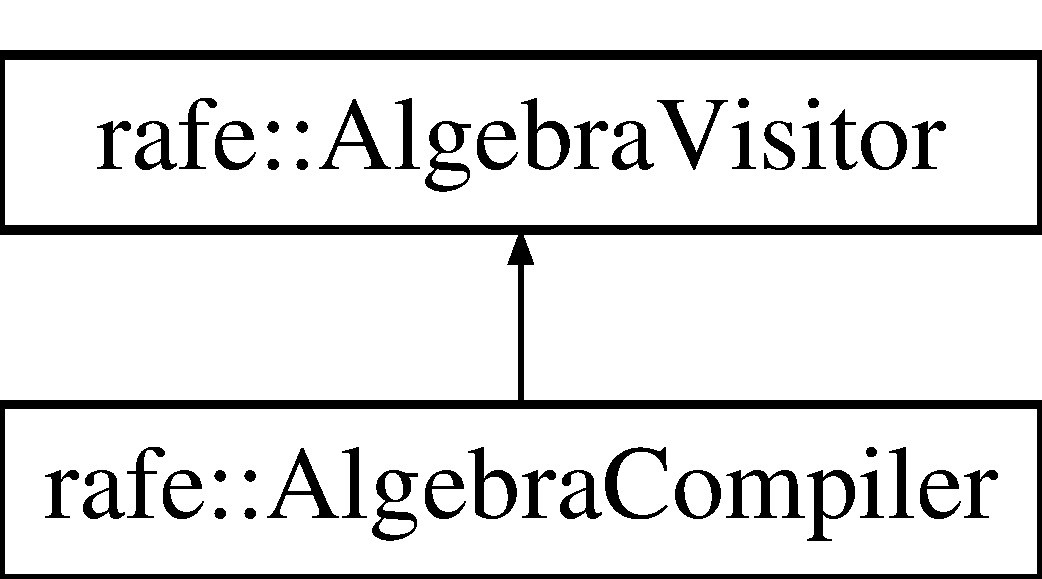
\includegraphics[height=2.000000cm]{classrafe_1_1_algebra_compiler}
\end{center}
\end{figure}
\subsection*{Public Member Functions}
\begin{DoxyCompactItemize}
\item 
void \hyperlink{classrafe_1_1_algebra_compiler_a43a2ccba61cff72a175c2fbd9c504c1d}{visit\+Table} (\hyperlink{classrafe_1_1_table}{Table} $\ast$node)
\item 
void \hyperlink{classrafe_1_1_algebra_compiler_a429613557ab8740d498228cadeaee07b}{visit\+Sort} (\hyperlink{classrafe_1_1_sort}{Sort} $\ast$node)
\item 
void \hyperlink{classrafe_1_1_algebra_compiler_ab910050702462e1437d148260d002e83}{visit\+Group} (\hyperlink{classrafe_1_1_group}{Group} $\ast$node)
\item 
void \hyperlink{classrafe_1_1_algebra_compiler_a89500aa1af613d82e231cba44eb0ccae}{visit\+Column\+Operations} (\hyperlink{classrafe_1_1_column_operations}{Column\+Operations} $\ast$node)
\item 
void \hyperlink{classrafe_1_1_algebra_compiler_ac74f4470af37f3a4d499bbfddf7aac9e}{visit\+Selection} (\hyperlink{classrafe_1_1_selection}{Selection} $\ast$node)
\item 
void \hyperlink{classrafe_1_1_algebra_compiler_a630e5f3fa963acae177df4f04fe99f1c}{visit\+Join} (\hyperlink{classrafe_1_1_join}{Join} $\ast$node)
\item 
void \hyperlink{classrafe_1_1_algebra_compiler_a605497973056e78786cdcf9ea621041c}{visit\+Anti\+Join} (\hyperlink{classrafe_1_1_anti_join}{Anti\+Join} $\ast$node)
\item 
void \hyperlink{classrafe_1_1_algebra_compiler_a325833b8f33d540a299df55def890d12}{visit\+Union} (\hyperlink{classrafe_1_1_union}{Union} $\ast$node)
\item 
void \hyperlink{classrafe_1_1_algebra_compiler_ab4eb22755e22796bf56cd03c0066b8b5}{visit\+Grouped\+Join} (\hyperlink{classrafe_1_1_grouped_join}{Grouped\+Join} $\ast$node)
\end{DoxyCompactItemize}
\subsection*{Static Public Member Functions}
\begin{DoxyCompactItemize}
\item 
static void \hyperlink{classrafe_1_1_algebra_compiler_a022cd6fb926e97863aa302d8c85ba07c}{update\+Sort\+Parameters} (const \hyperlink{classrafe_1_1_possible_sort_parameters}{Possible\+Sort\+Parameters} \&possible\+Sort\+Parameters, std\+::shared\+\_\+ptr$<$ \hyperlink{classrafe_1_1_physical_plan}{Physical\+Plan} $>$ \&new\+Plan, std\+::map$<$ int, \hyperlink{classrafe_1_1_column_info}{Column\+Info} $>$ \&new\+Columns)
\end{DoxyCompactItemize}
\subsection*{Public Attributes}
\begin{DoxyCompactItemize}
\item 
std\+::vector$<$ std\+::shared\+\_\+ptr\\*
$<$ \hyperlink{classrafe_1_1_physical_plan}{Physical\+Plan} $>$ $>$ \hyperlink{classrafe_1_1_algebra_compiler_a10ef60b632a1f593c0bbe3bbf5c3263c}{result}
\end{DoxyCompactItemize}
\subsection*{Static Public Attributes}
\begin{DoxyCompactItemize}
\item 
static const ulong \hyperlink{classrafe_1_1_algebra_compiler_afe381cc19b6dc860178b4a8783b51237}{N\+U\+M\+B\+E\+R\+\_\+\+O\+F\+\_\+\+P\+L\+A\+N\+S} = 5
\item 
static const ulong \hyperlink{classrafe_1_1_algebra_compiler_a576956fab718e7571201ffa24934b000}{L\+I\+M\+I\+T\+\_\+\+F\+O\+R\+\_\+\+G\+R\+E\+E\+D\+Y\+\_\+\+J\+O\+I\+N\+\_\+\+O\+R\+D\+E\+R\+\_\+\+A\+L\+G\+O\+R\+I\+T\+H\+M} = 5
\item 
static const ulong \hyperlink{classrafe_1_1_algebra_compiler_a19d056b84b6ee3621cf98d0d32bce141}{M\+A\+X\+\_\+\+H\+E\+A\+P\+\_\+\+S\+I\+Z\+E\+\_\+\+I\+N\+\_\+\+G\+R\+E\+E\+D\+Y\+\_\+\+A\+L\+G\+O\+R\+I\+T\+H\+M} = 20
\end{DoxyCompactItemize}


\subsection{Detailed Description}
\hyperlink{classrafe_1_1_algebra_visitor}{Algebra\+Visitor} which compiles relational algebra into physical plan. It uses from down to up method and it saves costant number of best plans for current subtree. 

\subsection{Member Function Documentation}
\hypertarget{classrafe_1_1_algebra_compiler_a022cd6fb926e97863aa302d8c85ba07c}{\index{rafe\+::\+Algebra\+Compiler@{rafe\+::\+Algebra\+Compiler}!update\+Sort\+Parameters@{update\+Sort\+Parameters}}
\index{update\+Sort\+Parameters@{update\+Sort\+Parameters}!rafe\+::\+Algebra\+Compiler@{rafe\+::\+Algebra\+Compiler}}
\subsubsection[{update\+Sort\+Parameters}]{\setlength{\rightskip}{0pt plus 5cm}void rafe\+::\+Algebra\+Compiler\+::update\+Sort\+Parameters (
\begin{DoxyParamCaption}
\item[{const {\bf Possible\+Sort\+Parameters} \&}]{possible\+Sort\+Parameters, }
\item[{std\+::shared\+\_\+ptr$<$ {\bf Physical\+Plan} $>$ \&}]{new\+Plan, }
\item[{std\+::map$<$ int, {\bf Column\+Info} $>$ \&}]{new\+Columns}
\end{DoxyParamCaption}
)\hspace{0.3cm}{\ttfamily [static]}}}\label{classrafe_1_1_algebra_compiler_a022cd6fb926e97863aa302d8c85ba07c}
From possible paramers remove columns, which aren't in new\+Columns and stores them into new\+Plan. 
\begin{DoxyParams}{Parameters}
{\em possible\+Sort\+Parameters} & -\/ parameters to update \\
\hline
{\em new\+Plan} & -\/ \hyperlink{classrafe_1_1_physical_plan}{Physical\+Plan}, where to store result \\
\hline
{\em new\+Columns} & -\/ columns which stays in parameters \\
\hline
\end{DoxyParams}
\hypertarget{classrafe_1_1_algebra_compiler_a605497973056e78786cdcf9ea621041c}{\index{rafe\+::\+Algebra\+Compiler@{rafe\+::\+Algebra\+Compiler}!visit\+Anti\+Join@{visit\+Anti\+Join}}
\index{visit\+Anti\+Join@{visit\+Anti\+Join}!rafe\+::\+Algebra\+Compiler@{rafe\+::\+Algebra\+Compiler}}
\subsubsection[{visit\+Anti\+Join}]{\setlength{\rightskip}{0pt plus 5cm}void rafe\+::\+Algebra\+Compiler\+::visit\+Anti\+Join (
\begin{DoxyParamCaption}
\item[{{\bf Anti\+Join} $\ast$}]{node}
\end{DoxyParamCaption}
)\hspace{0.3cm}{\ttfamily [virtual]}}}\label{classrafe_1_1_algebra_compiler_a605497973056e78786cdcf9ea621041c}
Visits \hyperlink{classrafe_1_1_anti_join}{Anti\+Join} element. 
\begin{DoxyParams}{Parameters}
{\em node} & visited \hyperlink{classrafe_1_1_anti_join}{Anti\+Join}. \\
\hline
\end{DoxyParams}


Reimplemented from \hyperlink{classrafe_1_1_algebra_visitor_a8b31789473135aff92e900a6a7765eda}{rafe\+::\+Algebra\+Visitor}.

\hypertarget{classrafe_1_1_algebra_compiler_a89500aa1af613d82e231cba44eb0ccae}{\index{rafe\+::\+Algebra\+Compiler@{rafe\+::\+Algebra\+Compiler}!visit\+Column\+Operations@{visit\+Column\+Operations}}
\index{visit\+Column\+Operations@{visit\+Column\+Operations}!rafe\+::\+Algebra\+Compiler@{rafe\+::\+Algebra\+Compiler}}
\subsubsection[{visit\+Column\+Operations}]{\setlength{\rightskip}{0pt plus 5cm}void rafe\+::\+Algebra\+Compiler\+::visit\+Column\+Operations (
\begin{DoxyParamCaption}
\item[{{\bf Column\+Operations} $\ast$}]{node}
\end{DoxyParamCaption}
)\hspace{0.3cm}{\ttfamily [virtual]}}}\label{classrafe_1_1_algebra_compiler_a89500aa1af613d82e231cba44eb0ccae}
Visits \hyperlink{classrafe_1_1_column_operations}{Column\+Operations} element. 
\begin{DoxyParams}{Parameters}
{\em node} & visited \hyperlink{classrafe_1_1_column_operations}{Column\+Operations}. \\
\hline
\end{DoxyParams}


Reimplemented from \hyperlink{classrafe_1_1_algebra_visitor_a518ce4d12f874a6c2f1fb0bb961144f8}{rafe\+::\+Algebra\+Visitor}.

\hypertarget{classrafe_1_1_algebra_compiler_ab910050702462e1437d148260d002e83}{\index{rafe\+::\+Algebra\+Compiler@{rafe\+::\+Algebra\+Compiler}!visit\+Group@{visit\+Group}}
\index{visit\+Group@{visit\+Group}!rafe\+::\+Algebra\+Compiler@{rafe\+::\+Algebra\+Compiler}}
\subsubsection[{visit\+Group}]{\setlength{\rightskip}{0pt plus 5cm}void rafe\+::\+Algebra\+Compiler\+::visit\+Group (
\begin{DoxyParamCaption}
\item[{{\bf Group} $\ast$}]{node}
\end{DoxyParamCaption}
)\hspace{0.3cm}{\ttfamily [virtual]}}}\label{classrafe_1_1_algebra_compiler_ab910050702462e1437d148260d002e83}
Visits \hyperlink{classrafe_1_1_group}{Group} element. 
\begin{DoxyParams}{Parameters}
{\em node} & visited \hyperlink{classrafe_1_1_group}{Group}. \\
\hline
\end{DoxyParams}


Reimplemented from \hyperlink{classrafe_1_1_algebra_visitor_a976d80987756215e71178f4c1863c6c7}{rafe\+::\+Algebra\+Visitor}.

\hypertarget{classrafe_1_1_algebra_compiler_ab4eb22755e22796bf56cd03c0066b8b5}{\index{rafe\+::\+Algebra\+Compiler@{rafe\+::\+Algebra\+Compiler}!visit\+Grouped\+Join@{visit\+Grouped\+Join}}
\index{visit\+Grouped\+Join@{visit\+Grouped\+Join}!rafe\+::\+Algebra\+Compiler@{rafe\+::\+Algebra\+Compiler}}
\subsubsection[{visit\+Grouped\+Join}]{\setlength{\rightskip}{0pt plus 5cm}void rafe\+::\+Algebra\+Compiler\+::visit\+Grouped\+Join (
\begin{DoxyParamCaption}
\item[{{\bf Grouped\+Join} $\ast$}]{node}
\end{DoxyParamCaption}
)\hspace{0.3cm}{\ttfamily [virtual]}}}\label{classrafe_1_1_algebra_compiler_ab4eb22755e22796bf56cd03c0066b8b5}
Visits \hyperlink{classrafe_1_1_grouped_join}{Grouped\+Join} element. 
\begin{DoxyParams}{Parameters}
{\em node} & visited \hyperlink{classrafe_1_1_grouped_join}{Grouped\+Join}. \\
\hline
\end{DoxyParams}


Reimplemented from \hyperlink{classrafe_1_1_algebra_visitor_a0715ce3279fa1edc6e472667e7739b57}{rafe\+::\+Algebra\+Visitor}.

\hypertarget{classrafe_1_1_algebra_compiler_a630e5f3fa963acae177df4f04fe99f1c}{\index{rafe\+::\+Algebra\+Compiler@{rafe\+::\+Algebra\+Compiler}!visit\+Join@{visit\+Join}}
\index{visit\+Join@{visit\+Join}!rafe\+::\+Algebra\+Compiler@{rafe\+::\+Algebra\+Compiler}}
\subsubsection[{visit\+Join}]{\setlength{\rightskip}{0pt plus 5cm}void rafe\+::\+Algebra\+Compiler\+::visit\+Join (
\begin{DoxyParamCaption}
\item[{{\bf Join} $\ast$}]{node}
\end{DoxyParamCaption}
)\hspace{0.3cm}{\ttfamily [virtual]}}}\label{classrafe_1_1_algebra_compiler_a630e5f3fa963acae177df4f04fe99f1c}
Visits \hyperlink{classrafe_1_1_join}{Join} element. 
\begin{DoxyParams}{Parameters}
{\em node} & visited \hyperlink{classrafe_1_1_join}{Join}. \\
\hline
\end{DoxyParams}


Reimplemented from \hyperlink{classrafe_1_1_algebra_visitor_ab499694bc7ccd718c6f7a5c4f3d33f1c}{rafe\+::\+Algebra\+Visitor}.

\hypertarget{classrafe_1_1_algebra_compiler_ac74f4470af37f3a4d499bbfddf7aac9e}{\index{rafe\+::\+Algebra\+Compiler@{rafe\+::\+Algebra\+Compiler}!visit\+Selection@{visit\+Selection}}
\index{visit\+Selection@{visit\+Selection}!rafe\+::\+Algebra\+Compiler@{rafe\+::\+Algebra\+Compiler}}
\subsubsection[{visit\+Selection}]{\setlength{\rightskip}{0pt plus 5cm}void rafe\+::\+Algebra\+Compiler\+::visit\+Selection (
\begin{DoxyParamCaption}
\item[{{\bf Selection} $\ast$}]{node}
\end{DoxyParamCaption}
)\hspace{0.3cm}{\ttfamily [virtual]}}}\label{classrafe_1_1_algebra_compiler_ac74f4470af37f3a4d499bbfddf7aac9e}
Visits \hyperlink{classrafe_1_1_selection}{Selection} element. 
\begin{DoxyParams}{Parameters}
{\em node} & visited \hyperlink{classrafe_1_1_selection}{Selection}. \\
\hline
\end{DoxyParams}


Reimplemented from \hyperlink{classrafe_1_1_algebra_visitor_a81f691749cb29da00bee299c617b9044}{rafe\+::\+Algebra\+Visitor}.

\hypertarget{classrafe_1_1_algebra_compiler_a429613557ab8740d498228cadeaee07b}{\index{rafe\+::\+Algebra\+Compiler@{rafe\+::\+Algebra\+Compiler}!visit\+Sort@{visit\+Sort}}
\index{visit\+Sort@{visit\+Sort}!rafe\+::\+Algebra\+Compiler@{rafe\+::\+Algebra\+Compiler}}
\subsubsection[{visit\+Sort}]{\setlength{\rightskip}{0pt plus 5cm}void rafe\+::\+Algebra\+Compiler\+::visit\+Sort (
\begin{DoxyParamCaption}
\item[{{\bf Sort} $\ast$}]{node}
\end{DoxyParamCaption}
)\hspace{0.3cm}{\ttfamily [virtual]}}}\label{classrafe_1_1_algebra_compiler_a429613557ab8740d498228cadeaee07b}
Visits \hyperlink{classrafe_1_1_sort}{Sort} element. 
\begin{DoxyParams}{Parameters}
{\em node} & visited \hyperlink{classrafe_1_1_sort}{Sort}. \\
\hline
\end{DoxyParams}


Reimplemented from \hyperlink{classrafe_1_1_algebra_visitor_a836e2efd8ac77071ad2487f9a5ae772d}{rafe\+::\+Algebra\+Visitor}.

\hypertarget{classrafe_1_1_algebra_compiler_a43a2ccba61cff72a175c2fbd9c504c1d}{\index{rafe\+::\+Algebra\+Compiler@{rafe\+::\+Algebra\+Compiler}!visit\+Table@{visit\+Table}}
\index{visit\+Table@{visit\+Table}!rafe\+::\+Algebra\+Compiler@{rafe\+::\+Algebra\+Compiler}}
\subsubsection[{visit\+Table}]{\setlength{\rightskip}{0pt plus 5cm}void rafe\+::\+Algebra\+Compiler\+::visit\+Table (
\begin{DoxyParamCaption}
\item[{{\bf Table} $\ast$}]{node}
\end{DoxyParamCaption}
)\hspace{0.3cm}{\ttfamily [virtual]}}}\label{classrafe_1_1_algebra_compiler_a43a2ccba61cff72a175c2fbd9c504c1d}
Visits \hyperlink{classrafe_1_1_table}{Table} element. 
\begin{DoxyParams}{Parameters}
{\em node} & visited \hyperlink{classrafe_1_1_table}{Table}. \\
\hline
\end{DoxyParams}


Reimplemented from \hyperlink{classrafe_1_1_algebra_visitor_a941798202c3a94d5b9884edc875ea88e}{rafe\+::\+Algebra\+Visitor}.

\hypertarget{classrafe_1_1_algebra_compiler_a325833b8f33d540a299df55def890d12}{\index{rafe\+::\+Algebra\+Compiler@{rafe\+::\+Algebra\+Compiler}!visit\+Union@{visit\+Union}}
\index{visit\+Union@{visit\+Union}!rafe\+::\+Algebra\+Compiler@{rafe\+::\+Algebra\+Compiler}}
\subsubsection[{visit\+Union}]{\setlength{\rightskip}{0pt plus 5cm}void rafe\+::\+Algebra\+Compiler\+::visit\+Union (
\begin{DoxyParamCaption}
\item[{{\bf Union} $\ast$}]{node}
\end{DoxyParamCaption}
)\hspace{0.3cm}{\ttfamily [virtual]}}}\label{classrafe_1_1_algebra_compiler_a325833b8f33d540a299df55def890d12}
Visits \hyperlink{classrafe_1_1_union}{Union} element. 
\begin{DoxyParams}{Parameters}
{\em node} & visited \hyperlink{classrafe_1_1_union}{Union}. \\
\hline
\end{DoxyParams}


Reimplemented from \hyperlink{classrafe_1_1_algebra_visitor_a1f8a7cae040f5918e562741a136bb096}{rafe\+::\+Algebra\+Visitor}.



\subsection{Member Data Documentation}
\hypertarget{classrafe_1_1_algebra_compiler_a576956fab718e7571201ffa24934b000}{\index{rafe\+::\+Algebra\+Compiler@{rafe\+::\+Algebra\+Compiler}!L\+I\+M\+I\+T\+\_\+\+F\+O\+R\+\_\+\+G\+R\+E\+E\+D\+Y\+\_\+\+J\+O\+I\+N\+\_\+\+O\+R\+D\+E\+R\+\_\+\+A\+L\+G\+O\+R\+I\+T\+H\+M@{L\+I\+M\+I\+T\+\_\+\+F\+O\+R\+\_\+\+G\+R\+E\+E\+D\+Y\+\_\+\+J\+O\+I\+N\+\_\+\+O\+R\+D\+E\+R\+\_\+\+A\+L\+G\+O\+R\+I\+T\+H\+M}}
\index{L\+I\+M\+I\+T\+\_\+\+F\+O\+R\+\_\+\+G\+R\+E\+E\+D\+Y\+\_\+\+J\+O\+I\+N\+\_\+\+O\+R\+D\+E\+R\+\_\+\+A\+L\+G\+O\+R\+I\+T\+H\+M@{L\+I\+M\+I\+T\+\_\+\+F\+O\+R\+\_\+\+G\+R\+E\+E\+D\+Y\+\_\+\+J\+O\+I\+N\+\_\+\+O\+R\+D\+E\+R\+\_\+\+A\+L\+G\+O\+R\+I\+T\+H\+M}!rafe\+::\+Algebra\+Compiler@{rafe\+::\+Algebra\+Compiler}}
\subsubsection[{L\+I\+M\+I\+T\+\_\+\+F\+O\+R\+\_\+\+G\+R\+E\+E\+D\+Y\+\_\+\+J\+O\+I\+N\+\_\+\+O\+R\+D\+E\+R\+\_\+\+A\+L\+G\+O\+R\+I\+T\+H\+M}]{\setlength{\rightskip}{0pt plus 5cm}const ulong rafe\+::\+Algebra\+Compiler\+::\+L\+I\+M\+I\+T\+\_\+\+F\+O\+R\+\_\+\+G\+R\+E\+E\+D\+Y\+\_\+\+J\+O\+I\+N\+\_\+\+O\+R\+D\+E\+R\+\_\+\+A\+L\+G\+O\+R\+I\+T\+H\+M = 5\hspace{0.3cm}{\ttfamily [static]}}}\label{classrafe_1_1_algebra_compiler_a576956fab718e7571201ffa24934b000}
Determines maximal number of inputs in group join to uses brute force join order algorithm. Otherwise greedy algorithm is used. \hypertarget{classrafe_1_1_algebra_compiler_a19d056b84b6ee3621cf98d0d32bce141}{\index{rafe\+::\+Algebra\+Compiler@{rafe\+::\+Algebra\+Compiler}!M\+A\+X\+\_\+\+H\+E\+A\+P\+\_\+\+S\+I\+Z\+E\+\_\+\+I\+N\+\_\+\+G\+R\+E\+E\+D\+Y\+\_\+\+A\+L\+G\+O\+R\+I\+T\+H\+M@{M\+A\+X\+\_\+\+H\+E\+A\+P\+\_\+\+S\+I\+Z\+E\+\_\+\+I\+N\+\_\+\+G\+R\+E\+E\+D\+Y\+\_\+\+A\+L\+G\+O\+R\+I\+T\+H\+M}}
\index{M\+A\+X\+\_\+\+H\+E\+A\+P\+\_\+\+S\+I\+Z\+E\+\_\+\+I\+N\+\_\+\+G\+R\+E\+E\+D\+Y\+\_\+\+A\+L\+G\+O\+R\+I\+T\+H\+M@{M\+A\+X\+\_\+\+H\+E\+A\+P\+\_\+\+S\+I\+Z\+E\+\_\+\+I\+N\+\_\+\+G\+R\+E\+E\+D\+Y\+\_\+\+A\+L\+G\+O\+R\+I\+T\+H\+M}!rafe\+::\+Algebra\+Compiler@{rafe\+::\+Algebra\+Compiler}}
\subsubsection[{M\+A\+X\+\_\+\+H\+E\+A\+P\+\_\+\+S\+I\+Z\+E\+\_\+\+I\+N\+\_\+\+G\+R\+E\+E\+D\+Y\+\_\+\+A\+L\+G\+O\+R\+I\+T\+H\+M}]{\setlength{\rightskip}{0pt plus 5cm}const ulong rafe\+::\+Algebra\+Compiler\+::\+M\+A\+X\+\_\+\+H\+E\+A\+P\+\_\+\+S\+I\+Z\+E\+\_\+\+I\+N\+\_\+\+G\+R\+E\+E\+D\+Y\+\_\+\+A\+L\+G\+O\+R\+I\+T\+H\+M = 20\hspace{0.3cm}{\ttfamily [static]}}}\label{classrafe_1_1_algebra_compiler_a19d056b84b6ee3621cf98d0d32bce141}
Determines how many plans can be stored in greddy join algorithm. \hypertarget{classrafe_1_1_algebra_compiler_afe381cc19b6dc860178b4a8783b51237}{\index{rafe\+::\+Algebra\+Compiler@{rafe\+::\+Algebra\+Compiler}!N\+U\+M\+B\+E\+R\+\_\+\+O\+F\+\_\+\+P\+L\+A\+N\+S@{N\+U\+M\+B\+E\+R\+\_\+\+O\+F\+\_\+\+P\+L\+A\+N\+S}}
\index{N\+U\+M\+B\+E\+R\+\_\+\+O\+F\+\_\+\+P\+L\+A\+N\+S@{N\+U\+M\+B\+E\+R\+\_\+\+O\+F\+\_\+\+P\+L\+A\+N\+S}!rafe\+::\+Algebra\+Compiler@{rafe\+::\+Algebra\+Compiler}}
\subsubsection[{N\+U\+M\+B\+E\+R\+\_\+\+O\+F\+\_\+\+P\+L\+A\+N\+S}]{\setlength{\rightskip}{0pt plus 5cm}const ulong rafe\+::\+Algebra\+Compiler\+::\+N\+U\+M\+B\+E\+R\+\_\+\+O\+F\+\_\+\+P\+L\+A\+N\+S = 5\hspace{0.3cm}{\ttfamily [static]}}}\label{classrafe_1_1_algebra_compiler_afe381cc19b6dc860178b4a8783b51237}
Determines what number of plans are used from visited subtree. \hypertarget{classrafe_1_1_algebra_compiler_a10ef60b632a1f593c0bbe3bbf5c3263c}{\index{rafe\+::\+Algebra\+Compiler@{rafe\+::\+Algebra\+Compiler}!result@{result}}
\index{result@{result}!rafe\+::\+Algebra\+Compiler@{rafe\+::\+Algebra\+Compiler}}
\subsubsection[{result}]{\setlength{\rightskip}{0pt plus 5cm}std\+::vector$<$std\+::shared\+\_\+ptr$<${\bf Physical\+Plan}$>$ $>$ rafe\+::\+Algebra\+Compiler\+::result}}\label{classrafe_1_1_algebra_compiler_a10ef60b632a1f593c0bbe3bbf5c3263c}
Stores plans after processing subtree. 

The documentation for this class was generated from the following files\+:\begin{DoxyCompactItemize}
\item 
C\+:/\+Users/\+Marcel/\+Documents/\+Visual Studio 2012/\+Projects/\+Relational\+Query\+Evaluator/\+Relational\+Query\+Evaluator/Algebra\+Visitors.\+h\item 
C\+:/\+Users/\+Marcel/\+Documents/\+Visual Studio 2012/\+Projects/\+Relational\+Query\+Evaluator/\+Relational\+Query\+Evaluator/Algebra\+Compiler.\+cpp\end{DoxyCompactItemize}

\hypertarget{classrafe_1_1_algebra_node_base}{\section{rafe\+:\+:Algebra\+Node\+Base Class Reference}
\label{classrafe_1_1_algebra_node_base}\index{rafe\+::\+Algebra\+Node\+Base@{rafe\+::\+Algebra\+Node\+Base}}
}


{\ttfamily \#include $<$Algebra.\+h$>$}

Inheritance diagram for rafe\+:\+:Algebra\+Node\+Base\+:\begin{figure}[H]
\begin{center}
\leavevmode
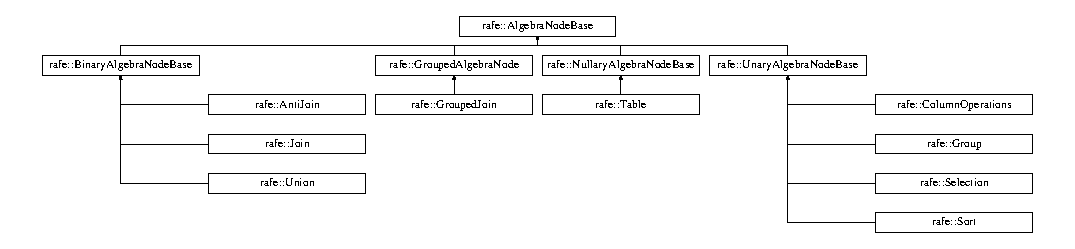
\includegraphics[height=2.901554cm]{classrafe_1_1_algebra_node_base}
\end{center}
\end{figure}
\subsection*{Public Member Functions}
\begin{DoxyCompactItemize}
\item 
\hyperlink{classrafe_1_1_algebra_node_base_a957999660bd1554dbfbc14ffaac4b8fe}{Algebra\+Node\+Base\+::\+Algebra\+Node\+Base} ()
\item 
\hyperlink{classrafe_1_1_algebra_node_base_a34676ea35550f991e09a646960ee98d0}{Algebra\+Node\+Base} (D\+O\+M\+Element $\ast$element)
\item 
\hyperlink{classrafe_1_1_algebra_node_base}{Algebra\+Node\+Base} $\ast$ \hyperlink{classrafe_1_1_algebra_node_base_a05bda55332729249965d5c09377e201f}{construct\+Children} (D\+O\+M\+Element $\ast$node)
\item 
virtual void \hyperlink{classrafe_1_1_algebra_node_base_a48e59b55cdb1c3d108343eb18920c1d1}{accept} (\hyperlink{classrafe_1_1_algebra_visitor}{Algebra\+Visitor} \&v)=0
\item 
virtual std\+::shared\+\_\+ptr\\*
$<$ \hyperlink{classrafe_1_1_algebra_node_base}{Algebra\+Node\+Base} $>$ \hyperlink{classrafe_1_1_algebra_node_base_ac6d722e739dd39c223bb129dfbd0ab45}{replace\+Child} (\hyperlink{classrafe_1_1_algebra_node_base}{Algebra\+Node\+Base} $\ast$old\+Child, std\+::shared\+\_\+ptr$<$ \hyperlink{classrafe_1_1_algebra_node_base}{Algebra\+Node\+Base} $>$ \&new\+Child)=0
\end{DoxyCompactItemize}
\subsection*{Public Attributes}
\begin{DoxyCompactItemize}
\item 
std\+::map$<$ int, \hyperlink{classrafe_1_1_column_info}{Column\+Info} $>$ \hyperlink{classrafe_1_1_algebra_node_base_aadae640fc5528efe6ce06c2171ba8075}{output\+Columns}
\item 
ulong \hyperlink{classrafe_1_1_algebra_node_base_a9ad122f37de5260754daaf517d3d5ed0}{line\+Number} = 0
\item 
\hyperlink{classrafe_1_1_algebra_node_base}{Algebra\+Node\+Base} $\ast$ \hyperlink{classrafe_1_1_algebra_node_base_a7dbfa2771e290b5e72bfe5c5177b7888}{parent}
\end{DoxyCompactItemize}


\subsection{Detailed Description}
Abstract class for algebraic operation. 

\subsection{Constructor \& Destructor Documentation}
\hypertarget{classrafe_1_1_algebra_node_base_a34676ea35550f991e09a646960ee98d0}{\index{rafe\+::\+Algebra\+Node\+Base@{rafe\+::\+Algebra\+Node\+Base}!Algebra\+Node\+Base@{Algebra\+Node\+Base}}
\index{Algebra\+Node\+Base@{Algebra\+Node\+Base}!rafe\+::\+Algebra\+Node\+Base@{rafe\+::\+Algebra\+Node\+Base}}
\subsubsection[{Algebra\+Node\+Base}]{\setlength{\rightskip}{0pt plus 5cm}rafe\+::\+Algebra\+Node\+Base\+::\+Algebra\+Node\+Base (
\begin{DoxyParamCaption}
\item[{D\+O\+M\+Element $\ast$}]{element}
\end{DoxyParamCaption}
)}}\label{classrafe_1_1_algebra_node_base_a34676ea35550f991e09a646960ee98d0}
Creates the instance of \hyperlink{classrafe_1_1_algebra_node_base}{Algebra\+Node\+Base}. 
\begin{DoxyParams}{Parameters}
{\em element} & representing input node. \\
\hline
\end{DoxyParams}


\subsection{Member Function Documentation}
\hypertarget{classrafe_1_1_algebra_node_base_a48e59b55cdb1c3d108343eb18920c1d1}{\index{rafe\+::\+Algebra\+Node\+Base@{rafe\+::\+Algebra\+Node\+Base}!accept@{accept}}
\index{accept@{accept}!rafe\+::\+Algebra\+Node\+Base@{rafe\+::\+Algebra\+Node\+Base}}
\subsubsection[{accept}]{\setlength{\rightskip}{0pt plus 5cm}virtual void rafe\+::\+Algebra\+Node\+Base\+::accept (
\begin{DoxyParamCaption}
\item[{{\bf Algebra\+Visitor} \&}]{v}
\end{DoxyParamCaption}
)\hspace{0.3cm}{\ttfamily [pure virtual]}}}\label{classrafe_1_1_algebra_node_base_a48e59b55cdb1c3d108343eb18920c1d1}
Method for calling visit\mbox{[}node\mbox{]} on given \hyperlink{classrafe_1_1_algebra_visitor}{Algebra\+Visitor}. 
\begin{DoxyParams}{Parameters}
{\em v} & \hyperlink{classrafe_1_1_algebra_visitor}{Algebra\+Visitor} on which to call function. \\
\hline
\end{DoxyParams}


Implemented in \hyperlink{classrafe_1_1_grouped_join_a36b56821dc719728f1f9294e3f8d8849}{rafe\+::\+Grouped\+Join}, \hyperlink{classrafe_1_1_union_adea56515e9bdebf9c37dc3da2cabec75}{rafe\+::\+Union}, \hyperlink{classrafe_1_1_anti_join_a6f4599cefdf10f6966239a3307c98621}{rafe\+::\+Anti\+Join}, \hyperlink{classrafe_1_1_join_a980b203f7b31b44fc564c996fcf28e98}{rafe\+::\+Join}, \hyperlink{classrafe_1_1_selection_a7304eb319db31a5c8ecb56b33d58e1e3}{rafe\+::\+Selection}, \hyperlink{classrafe_1_1_column_operations_a3418a59f4befbb949bf14e08d9c7d895}{rafe\+::\+Column\+Operations}, \hyperlink{classrafe_1_1_group_ac2ef050b2a4c52f38cd7d5ab4bf52dfe}{rafe\+::\+Group}, \hyperlink{classrafe_1_1_sort_a275b43c089710e24876f332177ca49c5}{rafe\+::\+Sort}, \hyperlink{classrafe_1_1_table_a2a807fb6c8921673ba7adb62dd0a9f7c}{rafe\+::\+Table}, \hyperlink{classrafe_1_1_nullary_algebra_node_base_a4e1bc16e76d9e41a8fb575008d8f15e5}{rafe\+::\+Nullary\+Algebra\+Node\+Base}, \hyperlink{classrafe_1_1_grouped_algebra_node_abdb48442900d5560f815f4eb33ebeb04}{rafe\+::\+Grouped\+Algebra\+Node}, \hyperlink{classrafe_1_1_binary_algebra_node_base_a0c9c2fdbd7062bf0bf4587b9abc493b2}{rafe\+::\+Binary\+Algebra\+Node\+Base}, and \hyperlink{classrafe_1_1_unary_algebra_node_base_a6f554aad7250a0f15730d10ae24e4a79}{rafe\+::\+Unary\+Algebra\+Node\+Base}.

\hypertarget{classrafe_1_1_algebra_node_base_a957999660bd1554dbfbc14ffaac4b8fe}{\index{rafe\+::\+Algebra\+Node\+Base@{rafe\+::\+Algebra\+Node\+Base}!Algebra\+Node\+Base\+::\+Algebra\+Node\+Base@{Algebra\+Node\+Base\+::\+Algebra\+Node\+Base}}
\index{Algebra\+Node\+Base\+::\+Algebra\+Node\+Base@{Algebra\+Node\+Base\+::\+Algebra\+Node\+Base}!rafe\+::\+Algebra\+Node\+Base@{rafe\+::\+Algebra\+Node\+Base}}
\subsubsection[{Algebra\+Node\+Base\+::\+Algebra\+Node\+Base}]{\setlength{\rightskip}{0pt plus 5cm}rafe\+::\+Algebra\+Node\+Base\+::\+Algebra\+Node\+Base\+::\+Algebra\+Node\+Base (
\begin{DoxyParamCaption}
{}
\end{DoxyParamCaption}
)}}\label{classrafe_1_1_algebra_node_base_a957999660bd1554dbfbc14ffaac4b8fe}
Creates the instance of \hyperlink{classrafe_1_1_algebra_node_base}{Algebra\+Node\+Base}. \hypertarget{classrafe_1_1_algebra_node_base_a05bda55332729249965d5c09377e201f}{\index{rafe\+::\+Algebra\+Node\+Base@{rafe\+::\+Algebra\+Node\+Base}!construct\+Children@{construct\+Children}}
\index{construct\+Children@{construct\+Children}!rafe\+::\+Algebra\+Node\+Base@{rafe\+::\+Algebra\+Node\+Base}}
\subsubsection[{construct\+Children}]{\setlength{\rightskip}{0pt plus 5cm}{\bf Algebra\+Node\+Base} $\ast$ rafe\+::\+Algebra\+Node\+Base\+::construct\+Children (
\begin{DoxyParamCaption}
\item[{D\+O\+M\+Element $\ast$}]{node}
\end{DoxyParamCaption}
)}}\label{classrafe_1_1_algebra_node_base_a05bda55332729249965d5c09377e201f}
Helper method for creating algebra tree from D\+O\+M tree. 
\begin{DoxyParams}{Parameters}
{\em node} & representing input node. \\
\hline
\end{DoxyParams}
\begin{DoxyReturn}{Returns}
newely created Algebra node. 
\end{DoxyReturn}
\hypertarget{classrafe_1_1_algebra_node_base_ac6d722e739dd39c223bb129dfbd0ab45}{\index{rafe\+::\+Algebra\+Node\+Base@{rafe\+::\+Algebra\+Node\+Base}!replace\+Child@{replace\+Child}}
\index{replace\+Child@{replace\+Child}!rafe\+::\+Algebra\+Node\+Base@{rafe\+::\+Algebra\+Node\+Base}}
\subsubsection[{replace\+Child}]{\setlength{\rightskip}{0pt plus 5cm}virtual std\+::shared\+\_\+ptr$<${\bf Algebra\+Node\+Base}$>$ rafe\+::\+Algebra\+Node\+Base\+::replace\+Child (
\begin{DoxyParamCaption}
\item[{{\bf Algebra\+Node\+Base} $\ast$}]{old\+Child, }
\item[{std\+::shared\+\_\+ptr$<$ {\bf Algebra\+Node\+Base} $>$ \&}]{new\+Child}
\end{DoxyParamCaption}
)\hspace{0.3cm}{\ttfamily [pure virtual]}}}\label{classrafe_1_1_algebra_node_base_ac6d722e739dd39c223bb129dfbd0ab45}
Replaces one child of this node with other one. 
\begin{DoxyParams}{Parameters}
{\em old\+Child} & node to be replaced. \\
\hline
{\em new\+Child} & new node to replace the old one. \\
\hline
\end{DoxyParams}
\begin{DoxyReturn}{Returns}
replaced child. 
\end{DoxyReturn}


Implemented in \hyperlink{classrafe_1_1_nullary_algebra_node_base_aa600eac4377bac4699834b0fbf1a4051}{rafe\+::\+Nullary\+Algebra\+Node\+Base}, \hyperlink{classrafe_1_1_grouped_algebra_node_a3e19a9a32840f4deebec342963955634}{rafe\+::\+Grouped\+Algebra\+Node}, \hyperlink{classrafe_1_1_binary_algebra_node_base_a7054bc98c4cca15927a326418e532d66}{rafe\+::\+Binary\+Algebra\+Node\+Base}, and \hyperlink{classrafe_1_1_unary_algebra_node_base_a32662d50e21fdc214d8acceb7e1029cc}{rafe\+::\+Unary\+Algebra\+Node\+Base}.



\subsection{Member Data Documentation}
\hypertarget{classrafe_1_1_algebra_node_base_a9ad122f37de5260754daaf517d3d5ed0}{\index{rafe\+::\+Algebra\+Node\+Base@{rafe\+::\+Algebra\+Node\+Base}!line\+Number@{line\+Number}}
\index{line\+Number@{line\+Number}!rafe\+::\+Algebra\+Node\+Base@{rafe\+::\+Algebra\+Node\+Base}}
\subsubsection[{line\+Number}]{\setlength{\rightskip}{0pt plus 5cm}ulong rafe\+::\+Algebra\+Node\+Base\+::line\+Number = 0}}\label{classrafe_1_1_algebra_node_base_a9ad122f37de5260754daaf517d3d5ed0}
Stores the line number of the input element for this node. \hypertarget{classrafe_1_1_algebra_node_base_aadae640fc5528efe6ce06c2171ba8075}{\index{rafe\+::\+Algebra\+Node\+Base@{rafe\+::\+Algebra\+Node\+Base}!output\+Columns@{output\+Columns}}
\index{output\+Columns@{output\+Columns}!rafe\+::\+Algebra\+Node\+Base@{rafe\+::\+Algebra\+Node\+Base}}
\subsubsection[{output\+Columns}]{\setlength{\rightskip}{0pt plus 5cm}std\+::map$<$int, {\bf Column\+Info}$>$ rafe\+::\+Algebra\+Node\+Base\+::output\+Columns}}\label{classrafe_1_1_algebra_node_base_aadae640fc5528efe6ce06c2171ba8075}
Stores ouput columns of this node. Map key is unique column identifier and map stores the information about column. \hypertarget{classrafe_1_1_algebra_node_base_a7dbfa2771e290b5e72bfe5c5177b7888}{\index{rafe\+::\+Algebra\+Node\+Base@{rafe\+::\+Algebra\+Node\+Base}!parent@{parent}}
\index{parent@{parent}!rafe\+::\+Algebra\+Node\+Base@{rafe\+::\+Algebra\+Node\+Base}}
\subsubsection[{parent}]{\setlength{\rightskip}{0pt plus 5cm}{\bf Algebra\+Node\+Base}$\ast$ rafe\+::\+Algebra\+Node\+Base\+::parent}}\label{classrafe_1_1_algebra_node_base_a7dbfa2771e290b5e72bfe5c5177b7888}
Stores the pointer on parent in the algebra tree. 

The documentation for this class was generated from the following files\+:\begin{DoxyCompactItemize}
\item 
C\+:/\+Users/\+Marcel/\+Documents/\+Visual Studio 2012/\+Projects/\+Relational\+Query\+Evaluator/\+Relational\+Query\+Evaluator/Algebra.\+h\item 
C\+:/\+Users/\+Marcel/\+Documents/\+Visual Studio 2012/\+Projects/\+Relational\+Query\+Evaluator/\+Relational\+Query\+Evaluator/Algebra.\+cpp\end{DoxyCompactItemize}

\hypertarget{classrafe_1_1_algebra_visitor}{\section{rafe\+:\+:Algebra\+Visitor Class Reference}
\label{classrafe_1_1_algebra_visitor}\index{rafe\+::\+Algebra\+Visitor@{rafe\+::\+Algebra\+Visitor}}
}


{\ttfamily \#include $<$Algebra\+Visitors.\+h$>$}

Inheritance diagram for rafe\+:\+:Algebra\+Visitor\+:\begin{figure}[H]
\begin{center}
\leavevmode
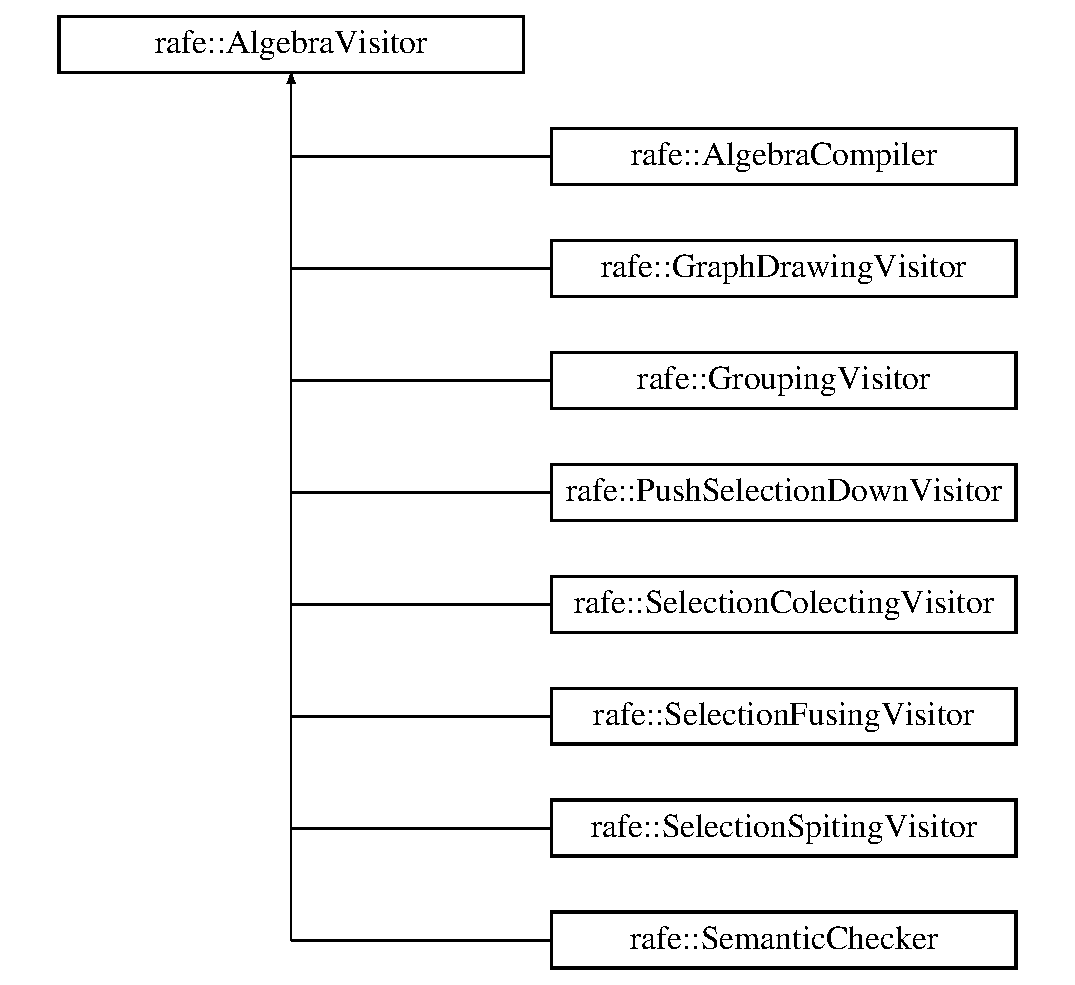
\includegraphics[height=9.000000cm]{classrafe_1_1_algebra_visitor}
\end{center}
\end{figure}
\subsection*{Public Member Functions}
\begin{DoxyCompactItemize}
\item 
virtual void \hyperlink{classrafe_1_1_algebra_visitor_a941798202c3a94d5b9884edc875ea88e}{visit\+Table} (\hyperlink{classrafe_1_1_table}{Table} $\ast$node)
\item 
virtual void \hyperlink{classrafe_1_1_algebra_visitor_a836e2efd8ac77071ad2487f9a5ae772d}{visit\+Sort} (\hyperlink{classrafe_1_1_sort}{Sort} $\ast$node)
\item 
virtual void \hyperlink{classrafe_1_1_algebra_visitor_a976d80987756215e71178f4c1863c6c7}{visit\+Group} (\hyperlink{classrafe_1_1_group}{Group} $\ast$node)
\item 
virtual void \hyperlink{classrafe_1_1_algebra_visitor_a518ce4d12f874a6c2f1fb0bb961144f8}{visit\+Column\+Operations} (\hyperlink{classrafe_1_1_column_operations}{Column\+Operations} $\ast$node)
\item 
virtual void \hyperlink{classrafe_1_1_algebra_visitor_a81f691749cb29da00bee299c617b9044}{visit\+Selection} (\hyperlink{classrafe_1_1_selection}{Selection} $\ast$node)
\item 
virtual void \hyperlink{classrafe_1_1_algebra_visitor_ab499694bc7ccd718c6f7a5c4f3d33f1c}{visit\+Join} (\hyperlink{classrafe_1_1_join}{Join} $\ast$node)
\item 
virtual void \hyperlink{classrafe_1_1_algebra_visitor_a8b31789473135aff92e900a6a7765eda}{visit\+Anti\+Join} (\hyperlink{classrafe_1_1_anti_join}{Anti\+Join} $\ast$node)
\item 
virtual void \hyperlink{classrafe_1_1_algebra_visitor_a1f8a7cae040f5918e562741a136bb096}{visit\+Union} (\hyperlink{classrafe_1_1_union}{Union} $\ast$node)
\item 
virtual void \hyperlink{classrafe_1_1_algebra_visitor_a0715ce3279fa1edc6e472667e7739b57}{visit\+Grouped\+Join} (\hyperlink{classrafe_1_1_grouped_join}{Grouped\+Join} $\ast$node)
\end{DoxyCompactItemize}
\subsection*{Static Public Member Functions}
\begin{DoxyCompactItemize}
\item 
static void \hyperlink{classrafe_1_1_algebra_visitor_a9d363c344928367680e60d1f7606ad06}{serialize\+Expression} (std\+::shared\+\_\+ptr$<$ \hyperlink{classrafe_1_1_expression}{Expression} $>$ \&condition, std\+::vector$<$ std\+::shared\+\_\+ptr$<$ \hyperlink{classrafe_1_1_expression}{Expression} $>$ $>$ \&result)
\item 
static std\+::shared\+\_\+ptr\\*
$<$ \hyperlink{classrafe_1_1_expression}{Expression} $>$ \hyperlink{classrafe_1_1_algebra_visitor_aee992f1216f75570dc7073f5031ecf7f}{deserialize\+Expression} (const std\+::vector$<$ std\+::shared\+\_\+ptr$<$ \hyperlink{classrafe_1_1_expression}{Expression} $>$ $>$ \&condition)
\item 
static void \hyperlink{classrafe_1_1_algebra_visitor_a1de5a4866096b3da07f921d351f437e7}{remove\+Selection} (\hyperlink{classrafe_1_1_selection}{Selection} $\ast$node)
\item 
static void \hyperlink{classrafe_1_1_algebra_visitor_a4eb384d25bff8d19c3d0d7310d33bf81}{insert\+Selection} (\hyperlink{classrafe_1_1_algebra_node_base}{Algebra\+Node\+Base} $\ast$node, std\+::shared\+\_\+ptr$<$ \hyperlink{classrafe_1_1_selection}{Selection} $>$ \&selection)
\end{DoxyCompactItemize}


\subsection{Detailed Description}
Base class for algebra tree visitors. Every virtual method does nothing, it only visits all children of the current node. 

\subsection{Member Function Documentation}
\hypertarget{classrafe_1_1_algebra_visitor_aee992f1216f75570dc7073f5031ecf7f}{\index{rafe\+::\+Algebra\+Visitor@{rafe\+::\+Algebra\+Visitor}!deserialize\+Expression@{deserialize\+Expression}}
\index{deserialize\+Expression@{deserialize\+Expression}!rafe\+::\+Algebra\+Visitor@{rafe\+::\+Algebra\+Visitor}}
\subsubsection[{deserialize\+Expression}]{\setlength{\rightskip}{0pt plus 5cm}shared\+\_\+ptr$<$ {\bf Expression} $>$ rafe\+::\+Algebra\+Visitor\+::deserialize\+Expression (
\begin{DoxyParamCaption}
\item[{const std\+::vector$<$ std\+::shared\+\_\+ptr$<$ {\bf Expression} $>$ $>$ \&}]{condition}
\end{DoxyParamCaption}
)\hspace{0.3cm}{\ttfamily [static]}}}\label{classrafe_1_1_algebra_visitor_aee992f1216f75570dc7073f5031ecf7f}
Convert expresion vector of subexpression to expression tree. 
\begin{DoxyParams}{Parameters}
{\em condition} & vector of \hyperlink{classrafe_1_1_expression}{Expression} \\
\hline
\end{DoxyParams}
\begin{DoxyReturn}{Returns}
tree condition 
\end{DoxyReturn}
\hypertarget{classrafe_1_1_algebra_visitor_a4eb384d25bff8d19c3d0d7310d33bf81}{\index{rafe\+::\+Algebra\+Visitor@{rafe\+::\+Algebra\+Visitor}!insert\+Selection@{insert\+Selection}}
\index{insert\+Selection@{insert\+Selection}!rafe\+::\+Algebra\+Visitor@{rafe\+::\+Algebra\+Visitor}}
\subsubsection[{insert\+Selection}]{\setlength{\rightskip}{0pt plus 5cm}void rafe\+::\+Algebra\+Visitor\+::insert\+Selection (
\begin{DoxyParamCaption}
\item[{{\bf Algebra\+Node\+Base} $\ast$}]{node, }
\item[{std\+::shared\+\_\+ptr$<$ {\bf Selection} $>$ \&}]{selection}
\end{DoxyParamCaption}
)\hspace{0.3cm}{\ttfamily [static]}}}\label{classrafe_1_1_algebra_visitor_a4eb384d25bff8d19c3d0d7310d33bf81}
Insert selection into the tree. New node will be inserted as parent of the first argument. 
\begin{DoxyParams}{Parameters}
{\em node} & \hyperlink{classrafe_1_1_algebra_node_base}{Algebra\+Node\+Base} where new node will be inserted \\
\hline
{\em selection} & -\/ \hyperlink{classrafe_1_1_selection}{Selection} to be inserted \\
\hline
\end{DoxyParams}
\hypertarget{classrafe_1_1_algebra_visitor_a1de5a4866096b3da07f921d351f437e7}{\index{rafe\+::\+Algebra\+Visitor@{rafe\+::\+Algebra\+Visitor}!remove\+Selection@{remove\+Selection}}
\index{remove\+Selection@{remove\+Selection}!rafe\+::\+Algebra\+Visitor@{rafe\+::\+Algebra\+Visitor}}
\subsubsection[{remove\+Selection}]{\setlength{\rightskip}{0pt plus 5cm}void rafe\+::\+Algebra\+Visitor\+::remove\+Selection (
\begin{DoxyParamCaption}
\item[{{\bf Selection} $\ast$}]{node}
\end{DoxyParamCaption}
)\hspace{0.3cm}{\ttfamily [static]}}}\label{classrafe_1_1_algebra_visitor_a1de5a4866096b3da07f921d351f437e7}
Remove selection node from the tree. 
\begin{DoxyParams}{Parameters}
{\em node} & \hyperlink{classrafe_1_1_selection}{Selection} to be removed \\
\hline
\end{DoxyParams}
\hypertarget{classrafe_1_1_algebra_visitor_a9d363c344928367680e60d1f7606ad06}{\index{rafe\+::\+Algebra\+Visitor@{rafe\+::\+Algebra\+Visitor}!serialize\+Expression@{serialize\+Expression}}
\index{serialize\+Expression@{serialize\+Expression}!rafe\+::\+Algebra\+Visitor@{rafe\+::\+Algebra\+Visitor}}
\subsubsection[{serialize\+Expression}]{\setlength{\rightskip}{0pt plus 5cm}void rafe\+::\+Algebra\+Visitor\+::serialize\+Expression (
\begin{DoxyParamCaption}
\item[{std\+::shared\+\_\+ptr$<$ {\bf Expression} $>$ \&}]{condition, }
\item[{std\+::vector$<$ std\+::shared\+\_\+ptr$<$ {\bf Expression} $>$ $>$ \&}]{result}
\end{DoxyParamCaption}
)\hspace{0.3cm}{\ttfamily [static]}}}\label{classrafe_1_1_algebra_visitor_a9d363c344928367680e60d1f7606ad06}
Convert expresion from tree to the vector of subconditions. Condition will be split into subconditions which are connected with and. 
\begin{DoxyParams}{Parameters}
{\em condition} & \hyperlink{classrafe_1_1_expression}{Expression} to convert. \\
\hline
{\em result} & vector of \hyperlink{classrafe_1_1_expression}{Expression}. Result of the function will be stored in this variable. Input needs to be empty. \\
\hline
\end{DoxyParams}
\hypertarget{classrafe_1_1_algebra_visitor_a8b31789473135aff92e900a6a7765eda}{\index{rafe\+::\+Algebra\+Visitor@{rafe\+::\+Algebra\+Visitor}!visit\+Anti\+Join@{visit\+Anti\+Join}}
\index{visit\+Anti\+Join@{visit\+Anti\+Join}!rafe\+::\+Algebra\+Visitor@{rafe\+::\+Algebra\+Visitor}}
\subsubsection[{visit\+Anti\+Join}]{\setlength{\rightskip}{0pt plus 5cm}void rafe\+::\+Algebra\+Visitor\+::visit\+Anti\+Join (
\begin{DoxyParamCaption}
\item[{{\bf Anti\+Join} $\ast$}]{node}
\end{DoxyParamCaption}
)\hspace{0.3cm}{\ttfamily [virtual]}}}\label{classrafe_1_1_algebra_visitor_a8b31789473135aff92e900a6a7765eda}
Visits \hyperlink{classrafe_1_1_anti_join}{Anti\+Join} node. 
\begin{DoxyParams}{Parameters}
{\em node} & visited \hyperlink{classrafe_1_1_anti_join}{Anti\+Join}. \\
\hline
\end{DoxyParams}


Reimplemented in \hyperlink{classrafe_1_1_push_selection_down_visitor_ab291a0f8f4e2c3638562b2ab628f9ed9}{rafe\+::\+Push\+Selection\+Down\+Visitor}, \hyperlink{classrafe_1_1_algebra_compiler_a605497973056e78786cdcf9ea621041c}{rafe\+::\+Algebra\+Compiler}, \hyperlink{classrafe_1_1_grouping_visitor_aa5f7889f7fc5ec289d7ee1107b441c0c}{rafe\+::\+Grouping\+Visitor}, \hyperlink{classrafe_1_1_semantic_checker_a891dd859fe5e91bc5c62cf8deaf5dddd}{rafe\+::\+Semantic\+Checker}, and \hyperlink{classrafe_1_1_graph_drawing_visitor_ad21a6c42f42490a47ebb0b858a34f527}{rafe\+::\+Graph\+Drawing\+Visitor}.

\hypertarget{classrafe_1_1_algebra_visitor_a518ce4d12f874a6c2f1fb0bb961144f8}{\index{rafe\+::\+Algebra\+Visitor@{rafe\+::\+Algebra\+Visitor}!visit\+Column\+Operations@{visit\+Column\+Operations}}
\index{visit\+Column\+Operations@{visit\+Column\+Operations}!rafe\+::\+Algebra\+Visitor@{rafe\+::\+Algebra\+Visitor}}
\subsubsection[{visit\+Column\+Operations}]{\setlength{\rightskip}{0pt plus 5cm}void rafe\+::\+Algebra\+Visitor\+::visit\+Column\+Operations (
\begin{DoxyParamCaption}
\item[{{\bf Column\+Operations} $\ast$}]{node}
\end{DoxyParamCaption}
)\hspace{0.3cm}{\ttfamily [virtual]}}}\label{classrafe_1_1_algebra_visitor_a518ce4d12f874a6c2f1fb0bb961144f8}
Visits \hyperlink{classrafe_1_1_column_operations}{Column\+Operations} node. 
\begin{DoxyParams}{Parameters}
{\em node} & visited \hyperlink{classrafe_1_1_column_operations}{Column\+Operations}. \\
\hline
\end{DoxyParams}


Reimplemented in \hyperlink{classrafe_1_1_push_selection_down_visitor_a4e6aa36753bc28600ea0bebfb4e501fb}{rafe\+::\+Push\+Selection\+Down\+Visitor}, \hyperlink{classrafe_1_1_algebra_compiler_a89500aa1af613d82e231cba44eb0ccae}{rafe\+::\+Algebra\+Compiler}, \hyperlink{classrafe_1_1_grouping_visitor_acb0f1d2cd1d7432d812191841efc6f60}{rafe\+::\+Grouping\+Visitor}, \hyperlink{classrafe_1_1_semantic_checker_a367226c2e23e15030e30bebb614df22d}{rafe\+::\+Semantic\+Checker}, and \hyperlink{classrafe_1_1_graph_drawing_visitor_a9933ed338ece545335fbad4052bf0c13}{rafe\+::\+Graph\+Drawing\+Visitor}.

\hypertarget{classrafe_1_1_algebra_visitor_a976d80987756215e71178f4c1863c6c7}{\index{rafe\+::\+Algebra\+Visitor@{rafe\+::\+Algebra\+Visitor}!visit\+Group@{visit\+Group}}
\index{visit\+Group@{visit\+Group}!rafe\+::\+Algebra\+Visitor@{rafe\+::\+Algebra\+Visitor}}
\subsubsection[{visit\+Group}]{\setlength{\rightskip}{0pt plus 5cm}void rafe\+::\+Algebra\+Visitor\+::visit\+Group (
\begin{DoxyParamCaption}
\item[{{\bf Group} $\ast$}]{node}
\end{DoxyParamCaption}
)\hspace{0.3cm}{\ttfamily [virtual]}}}\label{classrafe_1_1_algebra_visitor_a976d80987756215e71178f4c1863c6c7}
Visits \hyperlink{classrafe_1_1_group}{Group} node. 
\begin{DoxyParams}{Parameters}
{\em node} & visited \hyperlink{classrafe_1_1_group}{Group}. \\
\hline
\end{DoxyParams}


Reimplemented in \hyperlink{classrafe_1_1_push_selection_down_visitor_adc69a8ddf6a81cdfb1ab4ea8b2cdaf6e}{rafe\+::\+Push\+Selection\+Down\+Visitor}, \hyperlink{classrafe_1_1_algebra_compiler_ab910050702462e1437d148260d002e83}{rafe\+::\+Algebra\+Compiler}, \hyperlink{classrafe_1_1_semantic_checker_a89e58cb0414ac7f9657f3d16940e43db}{rafe\+::\+Semantic\+Checker}, and \hyperlink{classrafe_1_1_graph_drawing_visitor_aad5e1614a18f3d7aed5933775f614abf}{rafe\+::\+Graph\+Drawing\+Visitor}.

\hypertarget{classrafe_1_1_algebra_visitor_a0715ce3279fa1edc6e472667e7739b57}{\index{rafe\+::\+Algebra\+Visitor@{rafe\+::\+Algebra\+Visitor}!visit\+Grouped\+Join@{visit\+Grouped\+Join}}
\index{visit\+Grouped\+Join@{visit\+Grouped\+Join}!rafe\+::\+Algebra\+Visitor@{rafe\+::\+Algebra\+Visitor}}
\subsubsection[{visit\+Grouped\+Join}]{\setlength{\rightskip}{0pt plus 5cm}void rafe\+::\+Algebra\+Visitor\+::visit\+Grouped\+Join (
\begin{DoxyParamCaption}
\item[{{\bf Grouped\+Join} $\ast$}]{node}
\end{DoxyParamCaption}
)\hspace{0.3cm}{\ttfamily [virtual]}}}\label{classrafe_1_1_algebra_visitor_a0715ce3279fa1edc6e472667e7739b57}
Visits \hyperlink{classrafe_1_1_grouped_join}{Grouped\+Join} node. 
\begin{DoxyParams}{Parameters}
{\em node} & visited \hyperlink{classrafe_1_1_grouped_join}{Grouped\+Join}. \\
\hline
\end{DoxyParams}


Reimplemented in \hyperlink{classrafe_1_1_push_selection_down_visitor_ab3b99f6ca0ffc272be2a328b3bc13e31}{rafe\+::\+Push\+Selection\+Down\+Visitor}, \hyperlink{classrafe_1_1_algebra_compiler_ab4eb22755e22796bf56cd03c0066b8b5}{rafe\+::\+Algebra\+Compiler}, \hyperlink{classrafe_1_1_semantic_checker_a7cbba65715bdac55de4eef68a6698e17}{rafe\+::\+Semantic\+Checker}, and \hyperlink{classrafe_1_1_graph_drawing_visitor_a71b14af8909a3fe79c117ee8c8580352}{rafe\+::\+Graph\+Drawing\+Visitor}.

\hypertarget{classrafe_1_1_algebra_visitor_ab499694bc7ccd718c6f7a5c4f3d33f1c}{\index{rafe\+::\+Algebra\+Visitor@{rafe\+::\+Algebra\+Visitor}!visit\+Join@{visit\+Join}}
\index{visit\+Join@{visit\+Join}!rafe\+::\+Algebra\+Visitor@{rafe\+::\+Algebra\+Visitor}}
\subsubsection[{visit\+Join}]{\setlength{\rightskip}{0pt plus 5cm}void rafe\+::\+Algebra\+Visitor\+::visit\+Join (
\begin{DoxyParamCaption}
\item[{{\bf Join} $\ast$}]{node}
\end{DoxyParamCaption}
)\hspace{0.3cm}{\ttfamily [virtual]}}}\label{classrafe_1_1_algebra_visitor_ab499694bc7ccd718c6f7a5c4f3d33f1c}
Visits \hyperlink{classrafe_1_1_join}{Join} node. 
\begin{DoxyParams}{Parameters}
{\em node} & visited \hyperlink{classrafe_1_1_join}{Join}. \\
\hline
\end{DoxyParams}


Reimplemented in \hyperlink{classrafe_1_1_push_selection_down_visitor_a97825d74e8407111b3c28b4cd5b139dc}{rafe\+::\+Push\+Selection\+Down\+Visitor}, \hyperlink{classrafe_1_1_algebra_compiler_a630e5f3fa963acae177df4f04fe99f1c}{rafe\+::\+Algebra\+Compiler}, \hyperlink{classrafe_1_1_grouping_visitor_a519732d6b549b84cd543ab61aa7630f1}{rafe\+::\+Grouping\+Visitor}, \hyperlink{classrafe_1_1_semantic_checker_a5723cd81b7f2ba5f425e6fccf49741bc}{rafe\+::\+Semantic\+Checker}, and \hyperlink{classrafe_1_1_graph_drawing_visitor_abcf9e0f8c7a305923282701a17f56a8e}{rafe\+::\+Graph\+Drawing\+Visitor}.

\hypertarget{classrafe_1_1_algebra_visitor_a81f691749cb29da00bee299c617b9044}{\index{rafe\+::\+Algebra\+Visitor@{rafe\+::\+Algebra\+Visitor}!visit\+Selection@{visit\+Selection}}
\index{visit\+Selection@{visit\+Selection}!rafe\+::\+Algebra\+Visitor@{rafe\+::\+Algebra\+Visitor}}
\subsubsection[{visit\+Selection}]{\setlength{\rightskip}{0pt plus 5cm}void rafe\+::\+Algebra\+Visitor\+::visit\+Selection (
\begin{DoxyParamCaption}
\item[{{\bf Selection} $\ast$}]{node}
\end{DoxyParamCaption}
)\hspace{0.3cm}{\ttfamily [virtual]}}}\label{classrafe_1_1_algebra_visitor_a81f691749cb29da00bee299c617b9044}
Visits \hyperlink{classrafe_1_1_selection}{Selection} node. 
\begin{DoxyParams}{Parameters}
{\em node} & visited \hyperlink{classrafe_1_1_selection}{Selection}. \\
\hline
\end{DoxyParams}


Reimplemented in \hyperlink{classrafe_1_1_push_selection_down_visitor_a437c6c29c1d52149650c7b1443915d58}{rafe\+::\+Push\+Selection\+Down\+Visitor}, \hyperlink{classrafe_1_1_selection_colecting_visitor_a6789a4d32c1bb3b4b67ed6aa92c456df}{rafe\+::\+Selection\+Colecting\+Visitor}, \hyperlink{classrafe_1_1_selection_fusing_visitor_a4f728e97bda224020772f6a7c7cbb775}{rafe\+::\+Selection\+Fusing\+Visitor}, \hyperlink{classrafe_1_1_selection_spiting_visitor_a3fe48e9c5e4c511a443d3cc7fe9c49ef}{rafe\+::\+Selection\+Spiting\+Visitor}, \hyperlink{classrafe_1_1_algebra_compiler_ac74f4470af37f3a4d499bbfddf7aac9e}{rafe\+::\+Algebra\+Compiler}, \hyperlink{classrafe_1_1_grouping_visitor_a7287bb0601e55028ef362604144eae23}{rafe\+::\+Grouping\+Visitor}, \hyperlink{classrafe_1_1_semantic_checker_ad595114561381dbadaa6f75fd553764b}{rafe\+::\+Semantic\+Checker}, and \hyperlink{classrafe_1_1_graph_drawing_visitor_a01be2fcea00f7b0d7d70fa3dd168156c}{rafe\+::\+Graph\+Drawing\+Visitor}.

\hypertarget{classrafe_1_1_algebra_visitor_a836e2efd8ac77071ad2487f9a5ae772d}{\index{rafe\+::\+Algebra\+Visitor@{rafe\+::\+Algebra\+Visitor}!visit\+Sort@{visit\+Sort}}
\index{visit\+Sort@{visit\+Sort}!rafe\+::\+Algebra\+Visitor@{rafe\+::\+Algebra\+Visitor}}
\subsubsection[{visit\+Sort}]{\setlength{\rightskip}{0pt plus 5cm}void rafe\+::\+Algebra\+Visitor\+::visit\+Sort (
\begin{DoxyParamCaption}
\item[{{\bf Sort} $\ast$}]{node}
\end{DoxyParamCaption}
)\hspace{0.3cm}{\ttfamily [virtual]}}}\label{classrafe_1_1_algebra_visitor_a836e2efd8ac77071ad2487f9a5ae772d}
Visits \hyperlink{classrafe_1_1_sort}{Sort} node. 
\begin{DoxyParams}{Parameters}
{\em node} & visited \hyperlink{classrafe_1_1_sort}{Sort}. \\
\hline
\end{DoxyParams}


Reimplemented in \hyperlink{classrafe_1_1_push_selection_down_visitor_a4ea8d60b4150cbd0e7f95bd24f551433}{rafe\+::\+Push\+Selection\+Down\+Visitor}, \hyperlink{classrafe_1_1_algebra_compiler_a429613557ab8740d498228cadeaee07b}{rafe\+::\+Algebra\+Compiler}, \hyperlink{classrafe_1_1_semantic_checker_adf3ce7d0f3aa6ae9630d561edc1b0348}{rafe\+::\+Semantic\+Checker}, and \hyperlink{classrafe_1_1_graph_drawing_visitor_a5ba892e7e9400af6d1d2f89a896babd8}{rafe\+::\+Graph\+Drawing\+Visitor}.

\hypertarget{classrafe_1_1_algebra_visitor_a941798202c3a94d5b9884edc875ea88e}{\index{rafe\+::\+Algebra\+Visitor@{rafe\+::\+Algebra\+Visitor}!visit\+Table@{visit\+Table}}
\index{visit\+Table@{visit\+Table}!rafe\+::\+Algebra\+Visitor@{rafe\+::\+Algebra\+Visitor}}
\subsubsection[{visit\+Table}]{\setlength{\rightskip}{0pt plus 5cm}void rafe\+::\+Algebra\+Visitor\+::visit\+Table (
\begin{DoxyParamCaption}
\item[{{\bf Table} $\ast$}]{node}
\end{DoxyParamCaption}
)\hspace{0.3cm}{\ttfamily [virtual]}}}\label{classrafe_1_1_algebra_visitor_a941798202c3a94d5b9884edc875ea88e}
Visits \hyperlink{classrafe_1_1_table}{Table} node. 
\begin{DoxyParams}{Parameters}
{\em node} & visited \hyperlink{classrafe_1_1_table}{Table}. \\
\hline
\end{DoxyParams}


Reimplemented in \hyperlink{classrafe_1_1_push_selection_down_visitor_a22d4efbe167182bb5815c3155e4dfb15}{rafe\+::\+Push\+Selection\+Down\+Visitor}, \hyperlink{classrafe_1_1_algebra_compiler_a43a2ccba61cff72a175c2fbd9c504c1d}{rafe\+::\+Algebra\+Compiler}, \hyperlink{classrafe_1_1_semantic_checker_a05c36f62e97b763b6b5ba3faeb79d0bf}{rafe\+::\+Semantic\+Checker}, and \hyperlink{classrafe_1_1_graph_drawing_visitor_af5badeaa3070842bac2bad0e5bc38092}{rafe\+::\+Graph\+Drawing\+Visitor}.

\hypertarget{classrafe_1_1_algebra_visitor_a1f8a7cae040f5918e562741a136bb096}{\index{rafe\+::\+Algebra\+Visitor@{rafe\+::\+Algebra\+Visitor}!visit\+Union@{visit\+Union}}
\index{visit\+Union@{visit\+Union}!rafe\+::\+Algebra\+Visitor@{rafe\+::\+Algebra\+Visitor}}
\subsubsection[{visit\+Union}]{\setlength{\rightskip}{0pt plus 5cm}void rafe\+::\+Algebra\+Visitor\+::visit\+Union (
\begin{DoxyParamCaption}
\item[{{\bf Union} $\ast$}]{node}
\end{DoxyParamCaption}
)\hspace{0.3cm}{\ttfamily [virtual]}}}\label{classrafe_1_1_algebra_visitor_a1f8a7cae040f5918e562741a136bb096}
Visits \hyperlink{classrafe_1_1_union}{Union} node. 
\begin{DoxyParams}{Parameters}
{\em node} & visited \hyperlink{classrafe_1_1_union}{Union}. \\
\hline
\end{DoxyParams}


Reimplemented in \hyperlink{classrafe_1_1_push_selection_down_visitor_aa46479b019c02a80571e1b676d1f0aea}{rafe\+::\+Push\+Selection\+Down\+Visitor}, \hyperlink{classrafe_1_1_algebra_compiler_a325833b8f33d540a299df55def890d12}{rafe\+::\+Algebra\+Compiler}, \hyperlink{classrafe_1_1_semantic_checker_a86d3f5970f8f0994411aef2410986a0c}{rafe\+::\+Semantic\+Checker}, and \hyperlink{classrafe_1_1_graph_drawing_visitor_a093a7d242525ae764e2790ea06c74a9e}{rafe\+::\+Graph\+Drawing\+Visitor}.



The documentation for this class was generated from the following files\+:\begin{DoxyCompactItemize}
\item 
C\+:/\+Users/\+Marcel/\+Documents/\+Visual Studio 2012/\+Projects/\+Relational\+Query\+Evaluator/\+Relational\+Query\+Evaluator/Algebra\+Visitors.\+h\item 
C\+:/\+Users/\+Marcel/\+Documents/\+Visual Studio 2012/\+Projects/\+Relational\+Query\+Evaluator/\+Relational\+Query\+Evaluator/Algebra\+Visitors.\+cpp\end{DoxyCompactItemize}

\hypertarget{classrafe_1_1_anti_join}{\section{rafe\+:\+:Anti\+Join Class Reference}
\label{classrafe_1_1_anti_join}\index{rafe\+::\+Anti\+Join@{rafe\+::\+Anti\+Join}}
}


{\ttfamily \#include $<$Algebra.\+h$>$}

Inheritance diagram for rafe\+:\+:Anti\+Join\+:\begin{figure}[H]
\begin{center}
\leavevmode
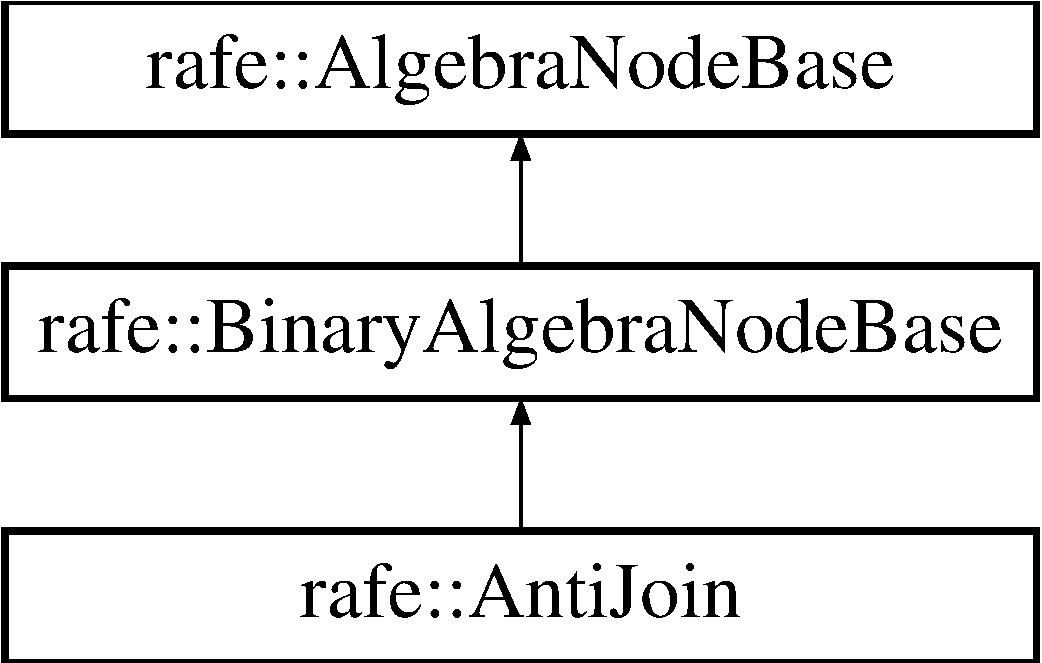
\includegraphics[height=3.000000cm]{classrafe_1_1_anti_join}
\end{center}
\end{figure}
\subsection*{Public Member Functions}
\begin{DoxyCompactItemize}
\item 
\hyperlink{classrafe_1_1_anti_join_a0f74edfc2442c9d091d15f4503702227}{Anti\+Join} (D\+O\+M\+Element $\ast$element)
\item 
void \hyperlink{classrafe_1_1_anti_join_a6f4599cefdf10f6966239a3307c98621}{accept} (\hyperlink{classrafe_1_1_algebra_visitor}{Algebra\+Visitor} \&v)
\end{DoxyCompactItemize}
\subsection*{Public Attributes}
\begin{DoxyCompactItemize}
\item 
std\+::shared\+\_\+ptr$<$ \hyperlink{classrafe_1_1_expression}{Expression} $>$ \hyperlink{classrafe_1_1_anti_join_a7eff7c54fb08dfefa4171080cd48fadc}{condition}
\item 
std\+::vector$<$ \hyperlink{classrafe_1_1_join_column_info}{Join\+Column\+Info} $>$ \hyperlink{classrafe_1_1_anti_join_a46d9e31d624610f99d6708fd5aee68be}{output\+Join\+Columns}
\end{DoxyCompactItemize}


\subsection{Detailed Description}
Represents algebraic operation antijoin. Antijoin is generalized difference and the columns of input do not have to be same. 

\subsection{Constructor \& Destructor Documentation}
\hypertarget{classrafe_1_1_anti_join_a0f74edfc2442c9d091d15f4503702227}{\index{rafe\+::\+Anti\+Join@{rafe\+::\+Anti\+Join}!Anti\+Join@{Anti\+Join}}
\index{Anti\+Join@{Anti\+Join}!rafe\+::\+Anti\+Join@{rafe\+::\+Anti\+Join}}
\subsubsection[{Anti\+Join}]{\setlength{\rightskip}{0pt plus 5cm}rafe\+::\+Anti\+Join\+::\+Anti\+Join (
\begin{DoxyParamCaption}
\item[{D\+O\+M\+Element $\ast$}]{element}
\end{DoxyParamCaption}
)}}\label{classrafe_1_1_anti_join_a0f74edfc2442c9d091d15f4503702227}
Creates the instance of \hyperlink{classrafe_1_1_anti_join}{Anti\+Join}. 
\begin{DoxyParams}{Parameters}
{\em element} & representing input node. \\
\hline
\end{DoxyParams}


\subsection{Member Function Documentation}
\hypertarget{classrafe_1_1_anti_join_a6f4599cefdf10f6966239a3307c98621}{\index{rafe\+::\+Anti\+Join@{rafe\+::\+Anti\+Join}!accept@{accept}}
\index{accept@{accept}!rafe\+::\+Anti\+Join@{rafe\+::\+Anti\+Join}}
\subsubsection[{accept}]{\setlength{\rightskip}{0pt plus 5cm}void rafe\+::\+Anti\+Join\+::accept (
\begin{DoxyParamCaption}
\item[{{\bf Algebra\+Visitor} \&}]{v}
\end{DoxyParamCaption}
)\hspace{0.3cm}{\ttfamily [virtual]}}}\label{classrafe_1_1_anti_join_a6f4599cefdf10f6966239a3307c98621}
Method for calling visit\mbox{[}node\mbox{]} on given \hyperlink{classrafe_1_1_algebra_visitor}{Algebra\+Visitor}. 
\begin{DoxyParams}{Parameters}
{\em v} & \hyperlink{classrafe_1_1_algebra_visitor}{Algebra\+Visitor} which to call function on \\
\hline
\end{DoxyParams}


Implements \hyperlink{classrafe_1_1_binary_algebra_node_base_a0c9c2fdbd7062bf0bf4587b9abc493b2}{rafe\+::\+Binary\+Algebra\+Node\+Base}.



\subsection{Member Data Documentation}
\hypertarget{classrafe_1_1_anti_join_a7eff7c54fb08dfefa4171080cd48fadc}{\index{rafe\+::\+Anti\+Join@{rafe\+::\+Anti\+Join}!condition@{condition}}
\index{condition@{condition}!rafe\+::\+Anti\+Join@{rafe\+::\+Anti\+Join}}
\subsubsection[{condition}]{\setlength{\rightskip}{0pt plus 5cm}std\+::shared\+\_\+ptr$<${\bf Expression}$>$ rafe\+::\+Anti\+Join\+::condition}}\label{classrafe_1_1_anti_join_a7eff7c54fb08dfefa4171080cd48fadc}
Condition for antijoin joining. \hypertarget{classrafe_1_1_anti_join_a46d9e31d624610f99d6708fd5aee68be}{\index{rafe\+::\+Anti\+Join@{rafe\+::\+Anti\+Join}!output\+Join\+Columns@{output\+Join\+Columns}}
\index{output\+Join\+Columns@{output\+Join\+Columns}!rafe\+::\+Anti\+Join@{rafe\+::\+Anti\+Join}}
\subsubsection[{output\+Join\+Columns}]{\setlength{\rightskip}{0pt plus 5cm}std\+::vector$<${\bf Join\+Column\+Info}$>$ rafe\+::\+Anti\+Join\+::output\+Join\+Columns}}\label{classrafe_1_1_anti_join_a46d9e31d624610f99d6708fd5aee68be}
List of join's output columns. 

The documentation for this class was generated from the following files\+:\begin{DoxyCompactItemize}
\item 
C\+:/\+Users/\+Marcel/\+Documents/\+Visual Studio 2012/\+Projects/\+Relational\+Query\+Evaluator/\+Relational\+Query\+Evaluator/Algebra.\+h\item 
C\+:/\+Users/\+Marcel/\+Documents/\+Visual Studio 2012/\+Projects/\+Relational\+Query\+Evaluator/\+Relational\+Query\+Evaluator/Algebra.\+cpp\end{DoxyCompactItemize}

\hypertarget{classrafe_1_1_binary_algebra_node_base}{\section{rafe\+:\+:Binary\+Algebra\+Node\+Base Class Reference}
\label{classrafe_1_1_binary_algebra_node_base}\index{rafe\+::\+Binary\+Algebra\+Node\+Base@{rafe\+::\+Binary\+Algebra\+Node\+Base}}
}


{\ttfamily \#include $<$Algebra.\+h$>$}

Inheritance diagram for rafe\+:\+:Binary\+Algebra\+Node\+Base\+:\begin{figure}[H]
\begin{center}
\leavevmode
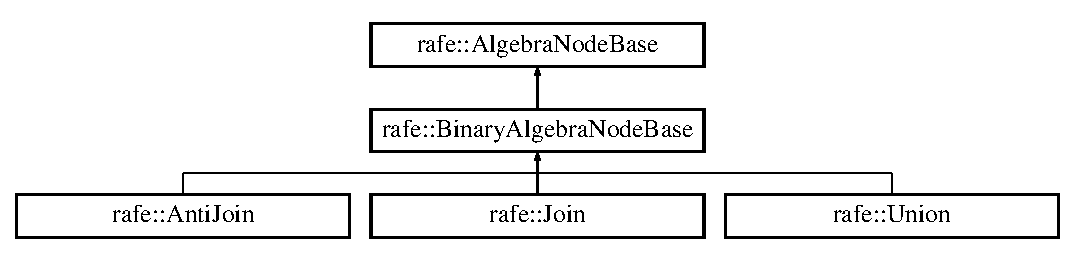
\includegraphics[height=2.962963cm]{classrafe_1_1_binary_algebra_node_base}
\end{center}
\end{figure}
\subsection*{Public Member Functions}
\begin{DoxyCompactItemize}
\item 
\hyperlink{classrafe_1_1_binary_algebra_node_base_a75ab2410e6296e01d27f500f250b6582}{Binary\+Algebra\+Node\+Base} ()
\item 
\hyperlink{classrafe_1_1_binary_algebra_node_base_a23b5bd89e39a5ee035a95aa7b4e1971c}{Binary\+Algebra\+Node\+Base} (D\+O\+M\+Element $\ast$element)
\item 
void \hyperlink{classrafe_1_1_binary_algebra_node_base_a614016d5d9dbf366eea5a4276c8e63b7}{construct\+Join\+Parameters} (D\+O\+M\+Element $\ast$node, std\+::shared\+\_\+ptr$<$ \hyperlink{classrafe_1_1_expression}{Expression} $>$ \&condition, std\+::vector$<$ \hyperlink{classrafe_1_1_join_column_info}{Join\+Column\+Info} $>$ \&\hyperlink{classrafe_1_1_algebra_node_base_aadae640fc5528efe6ce06c2171ba8075}{output\+Columns})
\item 
virtual void \hyperlink{classrafe_1_1_binary_algebra_node_base_a0c9c2fdbd7062bf0bf4587b9abc493b2}{accept} (\hyperlink{classrafe_1_1_algebra_visitor}{Algebra\+Visitor} \&v)=0
\item 
std\+::shared\+\_\+ptr$<$ \hyperlink{classrafe_1_1_algebra_node_base}{Algebra\+Node\+Base} $>$ \hyperlink{classrafe_1_1_binary_algebra_node_base_a7054bc98c4cca15927a326418e532d66}{replace\+Child} (\hyperlink{classrafe_1_1_algebra_node_base}{Algebra\+Node\+Base} $\ast$old\+Child, std\+::shared\+\_\+ptr$<$ \hyperlink{classrafe_1_1_algebra_node_base}{Algebra\+Node\+Base} $>$ \&new\+Child)
\end{DoxyCompactItemize}
\subsection*{Public Attributes}
\begin{DoxyCompactItemize}
\item 
std\+::shared\+\_\+ptr$<$ \hyperlink{classrafe_1_1_algebra_node_base}{Algebra\+Node\+Base} $>$ \hyperlink{classrafe_1_1_binary_algebra_node_base_af7380a182bdb21a519f3dd31ae189782}{left\+Child}
\item 
std\+::shared\+\_\+ptr$<$ \hyperlink{classrafe_1_1_algebra_node_base}{Algebra\+Node\+Base} $>$ \hyperlink{classrafe_1_1_binary_algebra_node_base_a147cbdd038dcd2f2fc5240e4594b3597}{right\+Child}
\end{DoxyCompactItemize}


\subsection{Detailed Description}
Abstract class for binary algebraic operation. 

\subsection{Constructor \& Destructor Documentation}
\hypertarget{classrafe_1_1_binary_algebra_node_base_a75ab2410e6296e01d27f500f250b6582}{\index{rafe\+::\+Binary\+Algebra\+Node\+Base@{rafe\+::\+Binary\+Algebra\+Node\+Base}!Binary\+Algebra\+Node\+Base@{Binary\+Algebra\+Node\+Base}}
\index{Binary\+Algebra\+Node\+Base@{Binary\+Algebra\+Node\+Base}!rafe\+::\+Binary\+Algebra\+Node\+Base@{rafe\+::\+Binary\+Algebra\+Node\+Base}}
\subsubsection[{Binary\+Algebra\+Node\+Base}]{\setlength{\rightskip}{0pt plus 5cm}rafe\+::\+Binary\+Algebra\+Node\+Base\+::\+Binary\+Algebra\+Node\+Base (
\begin{DoxyParamCaption}
{}
\end{DoxyParamCaption}
)}}\label{classrafe_1_1_binary_algebra_node_base_a75ab2410e6296e01d27f500f250b6582}
Creates the instance of \hyperlink{classrafe_1_1_binary_algebra_node_base}{Binary\+Algebra\+Node\+Base}. \hypertarget{classrafe_1_1_binary_algebra_node_base_a23b5bd89e39a5ee035a95aa7b4e1971c}{\index{rafe\+::\+Binary\+Algebra\+Node\+Base@{rafe\+::\+Binary\+Algebra\+Node\+Base}!Binary\+Algebra\+Node\+Base@{Binary\+Algebra\+Node\+Base}}
\index{Binary\+Algebra\+Node\+Base@{Binary\+Algebra\+Node\+Base}!rafe\+::\+Binary\+Algebra\+Node\+Base@{rafe\+::\+Binary\+Algebra\+Node\+Base}}
\subsubsection[{Binary\+Algebra\+Node\+Base}]{\setlength{\rightskip}{0pt plus 5cm}rafe\+::\+Binary\+Algebra\+Node\+Base\+::\+Binary\+Algebra\+Node\+Base (
\begin{DoxyParamCaption}
\item[{D\+O\+M\+Element $\ast$}]{element}
\end{DoxyParamCaption}
)}}\label{classrafe_1_1_binary_algebra_node_base_a23b5bd89e39a5ee035a95aa7b4e1971c}
Creates the instance of \hyperlink{classrafe_1_1_unary_algebra_node_base}{Unary\+Algebra\+Node\+Base}. 
\begin{DoxyParams}{Parameters}
{\em element} & representing input node. \\
\hline
\end{DoxyParams}


\subsection{Member Function Documentation}
\hypertarget{classrafe_1_1_binary_algebra_node_base_a0c9c2fdbd7062bf0bf4587b9abc493b2}{\index{rafe\+::\+Binary\+Algebra\+Node\+Base@{rafe\+::\+Binary\+Algebra\+Node\+Base}!accept@{accept}}
\index{accept@{accept}!rafe\+::\+Binary\+Algebra\+Node\+Base@{rafe\+::\+Binary\+Algebra\+Node\+Base}}
\subsubsection[{accept}]{\setlength{\rightskip}{0pt plus 5cm}virtual void rafe\+::\+Binary\+Algebra\+Node\+Base\+::accept (
\begin{DoxyParamCaption}
\item[{{\bf Algebra\+Visitor} \&}]{v}
\end{DoxyParamCaption}
)\hspace{0.3cm}{\ttfamily [pure virtual]}}}\label{classrafe_1_1_binary_algebra_node_base_a0c9c2fdbd7062bf0bf4587b9abc493b2}
Method for calling visit\mbox{[}node\mbox{]} on given \hyperlink{classrafe_1_1_algebra_visitor}{Algebra\+Visitor}. 
\begin{DoxyParams}{Parameters}
{\em v} & \hyperlink{classrafe_1_1_algebra_visitor}{Algebra\+Visitor} on which to call function. \\
\hline
\end{DoxyParams}


Implements \hyperlink{classrafe_1_1_algebra_node_base_a48e59b55cdb1c3d108343eb18920c1d1}{rafe\+::\+Algebra\+Node\+Base}.



Implemented in \hyperlink{classrafe_1_1_union_adea56515e9bdebf9c37dc3da2cabec75}{rafe\+::\+Union}, \hyperlink{classrafe_1_1_anti_join_a6f4599cefdf10f6966239a3307c98621}{rafe\+::\+Anti\+Join}, and \hyperlink{classrafe_1_1_join_a980b203f7b31b44fc564c996fcf28e98}{rafe\+::\+Join}.

\hypertarget{classrafe_1_1_binary_algebra_node_base_a614016d5d9dbf366eea5a4276c8e63b7}{\index{rafe\+::\+Binary\+Algebra\+Node\+Base@{rafe\+::\+Binary\+Algebra\+Node\+Base}!construct\+Join\+Parameters@{construct\+Join\+Parameters}}
\index{construct\+Join\+Parameters@{construct\+Join\+Parameters}!rafe\+::\+Binary\+Algebra\+Node\+Base@{rafe\+::\+Binary\+Algebra\+Node\+Base}}
\subsubsection[{construct\+Join\+Parameters}]{\setlength{\rightskip}{0pt plus 5cm}void rafe\+::\+Binary\+Algebra\+Node\+Base\+::construct\+Join\+Parameters (
\begin{DoxyParamCaption}
\item[{D\+O\+M\+Element $\ast$}]{node, }
\item[{std\+::shared\+\_\+ptr$<$ {\bf Expression} $>$ \&}]{condition, }
\item[{std\+::vector$<$ {\bf Join\+Column\+Info} $>$ \&}]{output\+Columns}
\end{DoxyParamCaption}
)}}\label{classrafe_1_1_binary_algebra_node_base_a614016d5d9dbf366eea5a4276c8e63b7}
Helper method for join and antijoin. Reads all needed parameters from D\+O\+M tree. 
\begin{DoxyParams}{Parameters}
{\em node} & -\/ input D\+O\+M element. \\
\hline
{\em condition} & -\/ output join condition. \\
\hline
{\em output\+Columns} & -\/ join output columns. \\
\hline
\end{DoxyParams}
\hypertarget{classrafe_1_1_binary_algebra_node_base_a7054bc98c4cca15927a326418e532d66}{\index{rafe\+::\+Binary\+Algebra\+Node\+Base@{rafe\+::\+Binary\+Algebra\+Node\+Base}!replace\+Child@{replace\+Child}}
\index{replace\+Child@{replace\+Child}!rafe\+::\+Binary\+Algebra\+Node\+Base@{rafe\+::\+Binary\+Algebra\+Node\+Base}}
\subsubsection[{replace\+Child}]{\setlength{\rightskip}{0pt plus 5cm}shared\+\_\+ptr$<$ {\bf Algebra\+Node\+Base} $>$ rafe\+::\+Binary\+Algebra\+Node\+Base\+::replace\+Child (
\begin{DoxyParamCaption}
\item[{{\bf Algebra\+Node\+Base} $\ast$}]{old\+Child, }
\item[{std\+::shared\+\_\+ptr$<$ {\bf Algebra\+Node\+Base} $>$ \&}]{new\+Child}
\end{DoxyParamCaption}
)\hspace{0.3cm}{\ttfamily [virtual]}}}\label{classrafe_1_1_binary_algebra_node_base_a7054bc98c4cca15927a326418e532d66}
Replaces one child of this node with other one. 
\begin{DoxyParams}{Parameters}
{\em old\+Child} & node to be replaced. \\
\hline
{\em new\+Child} & new node to replace the old one. \\
\hline
\end{DoxyParams}
\begin{DoxyReturn}{Returns}
replaced child. 
\end{DoxyReturn}


Implements \hyperlink{classrafe_1_1_algebra_node_base_ac6d722e739dd39c223bb129dfbd0ab45}{rafe\+::\+Algebra\+Node\+Base}.



\subsection{Member Data Documentation}
\hypertarget{classrafe_1_1_binary_algebra_node_base_af7380a182bdb21a519f3dd31ae189782}{\index{rafe\+::\+Binary\+Algebra\+Node\+Base@{rafe\+::\+Binary\+Algebra\+Node\+Base}!left\+Child@{left\+Child}}
\index{left\+Child@{left\+Child}!rafe\+::\+Binary\+Algebra\+Node\+Base@{rafe\+::\+Binary\+Algebra\+Node\+Base}}
\subsubsection[{left\+Child}]{\setlength{\rightskip}{0pt plus 5cm}std\+::shared\+\_\+ptr$<${\bf Algebra\+Node\+Base}$>$ rafe\+::\+Binary\+Algebra\+Node\+Base\+::left\+Child}}\label{classrafe_1_1_binary_algebra_node_base_af7380a182bdb21a519f3dd31ae189782}
Stores pointer to the left child node. \hypertarget{classrafe_1_1_binary_algebra_node_base_a147cbdd038dcd2f2fc5240e4594b3597}{\index{rafe\+::\+Binary\+Algebra\+Node\+Base@{rafe\+::\+Binary\+Algebra\+Node\+Base}!right\+Child@{right\+Child}}
\index{right\+Child@{right\+Child}!rafe\+::\+Binary\+Algebra\+Node\+Base@{rafe\+::\+Binary\+Algebra\+Node\+Base}}
\subsubsection[{right\+Child}]{\setlength{\rightskip}{0pt plus 5cm}std\+::shared\+\_\+ptr$<${\bf Algebra\+Node\+Base}$>$ rafe\+::\+Binary\+Algebra\+Node\+Base\+::right\+Child}}\label{classrafe_1_1_binary_algebra_node_base_a147cbdd038dcd2f2fc5240e4594b3597}
Stores pointer to the right child node. 

The documentation for this class was generated from the following files\+:\begin{DoxyCompactItemize}
\item 
C\+:/\+Users/\+Marcel/\+Documents/\+Visual Studio 2012/\+Projects/\+Relational\+Query\+Evaluator/\+Relational\+Query\+Evaluator/Algebra.\+h\item 
C\+:/\+Users/\+Marcel/\+Documents/\+Visual Studio 2012/\+Projects/\+Relational\+Query\+Evaluator/\+Relational\+Query\+Evaluator/Algebra.\+cpp\end{DoxyCompactItemize}

\hypertarget{classrafe_1_1_binary_expression}{\section{rafe\+:\+:Binary\+Expression Class Reference}
\label{classrafe_1_1_binary_expression}\index{rafe\+::\+Binary\+Expression@{rafe\+::\+Binary\+Expression}}
}


{\ttfamily \#include $<$Expressions.\+h$>$}

Inheritance diagram for rafe\+:\+:Binary\+Expression\+:\begin{figure}[H]
\begin{center}
\leavevmode
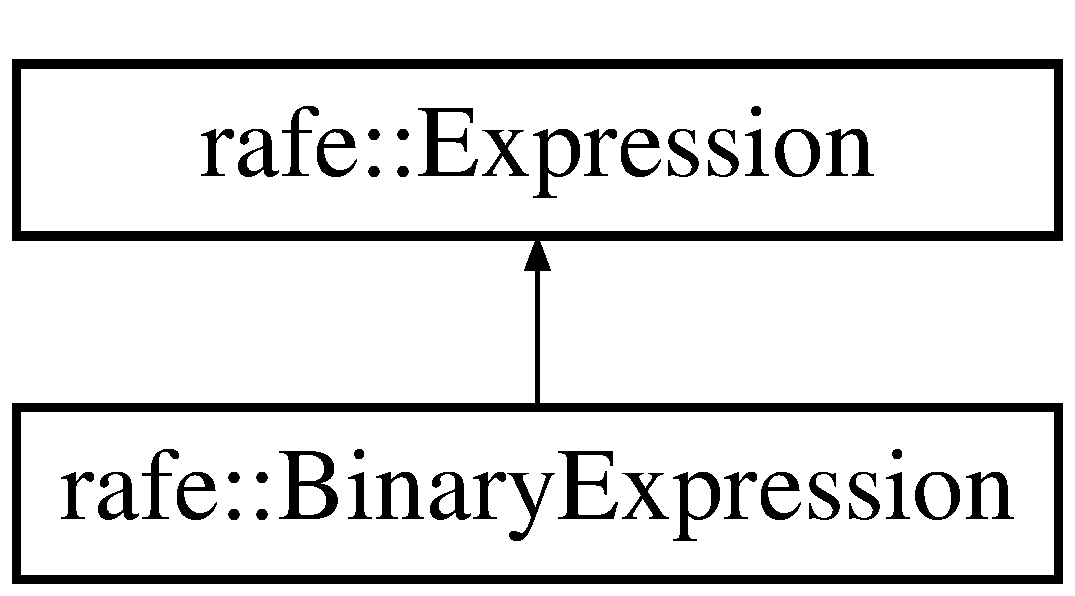
\includegraphics[height=2.000000cm]{classrafe_1_1_binary_expression}
\end{center}
\end{figure}
\subsection*{Public Member Functions}
\begin{DoxyCompactItemize}
\item 
\hyperlink{classrafe_1_1_binary_expression_a28a843c17e363547740ab7bdbc23c7f9}{Binary\+Expression} (D\+O\+M\+Element $\ast$node, Binary\+Operator op)
\item 
\hyperlink{classrafe_1_1_binary_expression_acd2ee559a5dfb360d8fab62186b8fbce}{Binary\+Expression} (std\+::shared\+\_\+ptr$<$ \hyperlink{classrafe_1_1_expression}{Expression} $>$ \&\hyperlink{classrafe_1_1_binary_expression_a1c428205f0d4d597a6307e7cab39ee21}{left\+Child}, std\+::shared\+\_\+ptr$<$ \hyperlink{classrafe_1_1_expression}{Expression} $>$ \&\hyperlink{classrafe_1_1_binary_expression_ad915f6160c53ad08803e30db1ffc8e1c}{right\+Child}, Binary\+Operator op)
\item 
void \hyperlink{classrafe_1_1_binary_expression_a343b5568f9fa7bf63b1f734bfed65f78}{accept} (\hyperlink{classrafe_1_1_expression_visitor_base}{Expression\+Visitor\+Base} \&v)
\item 
void \hyperlink{classrafe_1_1_binary_expression_ac094c4a5686ded1827d12e14bdfae1c6}{replace\+Child} (\hyperlink{classrafe_1_1_expression}{Expression} $\ast$old\+Child, std\+::shared\+\_\+ptr$<$ \hyperlink{classrafe_1_1_expression}{Expression} $>$ new\+Child)
\end{DoxyCompactItemize}
\subsection*{Public Attributes}
\begin{DoxyCompactItemize}
\item 
Binary\+Operator \hyperlink{classrafe_1_1_binary_expression_a7180ae7c20f907d52a0f9c8521d5c111}{operation}
\item 
std\+::shared\+\_\+ptr$<$ \hyperlink{classrafe_1_1_expression}{Expression} $>$ \hyperlink{classrafe_1_1_binary_expression_a1c428205f0d4d597a6307e7cab39ee21}{left\+Child}
\item 
std\+::shared\+\_\+ptr$<$ \hyperlink{classrafe_1_1_expression}{Expression} $>$ \hyperlink{classrafe_1_1_binary_expression_ad915f6160c53ad08803e30db1ffc8e1c}{right\+Child}
\end{DoxyCompactItemize}
\subsection*{Additional Inherited Members}


\subsection{Detailed Description}
Class representing binary expression (two children). It is used to store artimeric(+,-\/,$\ast$,/) and logic operations (and,or). 

\subsection{Constructor \& Destructor Documentation}
\hypertarget{classrafe_1_1_binary_expression_a28a843c17e363547740ab7bdbc23c7f9}{\index{rafe\+::\+Binary\+Expression@{rafe\+::\+Binary\+Expression}!Binary\+Expression@{Binary\+Expression}}
\index{Binary\+Expression@{Binary\+Expression}!rafe\+::\+Binary\+Expression@{rafe\+::\+Binary\+Expression}}
\subsubsection[{Binary\+Expression}]{\setlength{\rightskip}{0pt plus 5cm}rafe\+::\+Binary\+Expression\+::\+Binary\+Expression (
\begin{DoxyParamCaption}
\item[{D\+O\+M\+Element $\ast$}]{node, }
\item[{Binary\+Operator}]{op}
\end{DoxyParamCaption}
)}}\label{classrafe_1_1_binary_expression_a28a843c17e363547740ab7bdbc23c7f9}
Creates new instance of \hyperlink{classrafe_1_1_binary_expression}{Binary\+Expression} 
\begin{DoxyParams}{Parameters}
{\em node} & -\/ domelement hoding information about node and its child nodes. \\
\hline
{\em op} & -\/ type of binary operation \\
\hline
\end{DoxyParams}
\hypertarget{classrafe_1_1_binary_expression_acd2ee559a5dfb360d8fab62186b8fbce}{\index{rafe\+::\+Binary\+Expression@{rafe\+::\+Binary\+Expression}!Binary\+Expression@{Binary\+Expression}}
\index{Binary\+Expression@{Binary\+Expression}!rafe\+::\+Binary\+Expression@{rafe\+::\+Binary\+Expression}}
\subsubsection[{Binary\+Expression}]{\setlength{\rightskip}{0pt plus 5cm}rafe\+::\+Binary\+Expression\+::\+Binary\+Expression (
\begin{DoxyParamCaption}
\item[{std\+::shared\+\_\+ptr$<$ {\bf Expression} $>$ \&}]{left\+Child, }
\item[{std\+::shared\+\_\+ptr$<$ {\bf Expression} $>$ \&}]{right\+Child, }
\item[{Binary\+Operator}]{op}
\end{DoxyParamCaption}
)}}\label{classrafe_1_1_binary_expression_acd2ee559a5dfb360d8fab62186b8fbce}
Creates new instance of \hyperlink{classrafe_1_1_binary_expression}{Binary\+Expression}. 
\begin{DoxyParams}{Parameters}
{\em left\+Child} & -\/ new left child node \\
\hline
{\em right\+Child} & -\/ new right child node \\
\hline
{\em op} & -\/ type of binary operation \\
\hline
\end{DoxyParams}


\subsection{Member Function Documentation}
\hypertarget{classrafe_1_1_binary_expression_a343b5568f9fa7bf63b1f734bfed65f78}{\index{rafe\+::\+Binary\+Expression@{rafe\+::\+Binary\+Expression}!accept@{accept}}
\index{accept@{accept}!rafe\+::\+Binary\+Expression@{rafe\+::\+Binary\+Expression}}
\subsubsection[{accept}]{\setlength{\rightskip}{0pt plus 5cm}void rafe\+::\+Binary\+Expression\+::accept (
\begin{DoxyParamCaption}
\item[{{\bf Expression\+Visitor\+Base} \&}]{v}
\end{DoxyParamCaption}
)\hspace{0.3cm}{\ttfamily [virtual]}}}\label{classrafe_1_1_binary_expression_a343b5568f9fa7bf63b1f734bfed65f78}
Method for calling visit\mbox{[}node\mbox{]} on given Expression\+Visitor. 
\begin{DoxyParams}{Parameters}
{\em v} & Expression\+Visitor, on which to call visit function. \\
\hline
\end{DoxyParams}


Implements \hyperlink{classrafe_1_1_expression_a3b2e5bae8b99ea6c9a3c92a9b949b3cd}{rafe\+::\+Expression}.

\hypertarget{classrafe_1_1_binary_expression_ac094c4a5686ded1827d12e14bdfae1c6}{\index{rafe\+::\+Binary\+Expression@{rafe\+::\+Binary\+Expression}!replace\+Child@{replace\+Child}}
\index{replace\+Child@{replace\+Child}!rafe\+::\+Binary\+Expression@{rafe\+::\+Binary\+Expression}}
\subsubsection[{replace\+Child}]{\setlength{\rightskip}{0pt plus 5cm}void rafe\+::\+Binary\+Expression\+::replace\+Child (
\begin{DoxyParamCaption}
\item[{{\bf Expression} $\ast$}]{old\+Child, }
\item[{std\+::shared\+\_\+ptr$<$ {\bf Expression} $>$}]{new\+Child}
\end{DoxyParamCaption}
)\hspace{0.3cm}{\ttfamily [virtual]}}}\label{classrafe_1_1_binary_expression_ac094c4a5686ded1827d12e14bdfae1c6}
Replaces child from this class with new expression tree. 
\begin{DoxyParams}{Parameters}
{\em old\+Child} & -\/ child to replace. \\
\hline
{\em new\+Child} & -\/ child to be replaced. \\
\hline
\end{DoxyParams}


Implements \hyperlink{classrafe_1_1_expression_a841879e8eb85f4bb68cfeec24231a701}{rafe\+::\+Expression}.



\subsection{Member Data Documentation}
\hypertarget{classrafe_1_1_binary_expression_a1c428205f0d4d597a6307e7cab39ee21}{\index{rafe\+::\+Binary\+Expression@{rafe\+::\+Binary\+Expression}!left\+Child@{left\+Child}}
\index{left\+Child@{left\+Child}!rafe\+::\+Binary\+Expression@{rafe\+::\+Binary\+Expression}}
\subsubsection[{left\+Child}]{\setlength{\rightskip}{0pt plus 5cm}std\+::shared\+\_\+ptr$<${\bf Expression}$>$ rafe\+::\+Binary\+Expression\+::left\+Child}}\label{classrafe_1_1_binary_expression_a1c428205f0d4d597a6307e7cab39ee21}
Stores pointer to left child tree node. \hypertarget{classrafe_1_1_binary_expression_a7180ae7c20f907d52a0f9c8521d5c111}{\index{rafe\+::\+Binary\+Expression@{rafe\+::\+Binary\+Expression}!operation@{operation}}
\index{operation@{operation}!rafe\+::\+Binary\+Expression@{rafe\+::\+Binary\+Expression}}
\subsubsection[{operation}]{\setlength{\rightskip}{0pt plus 5cm}Binary\+Operator rafe\+::\+Binary\+Expression\+::operation}}\label{classrafe_1_1_binary_expression_a7180ae7c20f907d52a0f9c8521d5c111}
Stores infromation about type of binary operation. \hypertarget{classrafe_1_1_binary_expression_ad915f6160c53ad08803e30db1ffc8e1c}{\index{rafe\+::\+Binary\+Expression@{rafe\+::\+Binary\+Expression}!right\+Child@{right\+Child}}
\index{right\+Child@{right\+Child}!rafe\+::\+Binary\+Expression@{rafe\+::\+Binary\+Expression}}
\subsubsection[{right\+Child}]{\setlength{\rightskip}{0pt plus 5cm}std\+::shared\+\_\+ptr$<${\bf Expression}$>$ rafe\+::\+Binary\+Expression\+::right\+Child}}\label{classrafe_1_1_binary_expression_ad915f6160c53ad08803e30db1ffc8e1c}
Stores pointer to right child tree node. 

The documentation for this class was generated from the following files\+:\begin{DoxyCompactItemize}
\item 
C\+:/\+Users/\+Marcel/\+Documents/\+Visual Studio 2012/\+Projects/\+Relational\+Query\+Evaluator/\+Relational\+Query\+Evaluator/Expressions.\+h\item 
C\+:/\+Users/\+Marcel/\+Documents/\+Visual Studio 2012/\+Projects/\+Relational\+Query\+Evaluator/\+Relational\+Query\+Evaluator/Expressions.\+cpp\end{DoxyCompactItemize}

\hypertarget{classrafe_1_1_binary_physical_operator}{\section{rafe\+:\+:Binary\+Physical\+Operator Class Reference}
\label{classrafe_1_1_binary_physical_operator}\index{rafe\+::\+Binary\+Physical\+Operator@{rafe\+::\+Binary\+Physical\+Operator}}
}


{\ttfamily \#include $<$Physical\+Operator.\+h$>$}

Inheritance diagram for rafe\+:\+:Binary\+Physical\+Operator\+:\begin{figure}[H]
\begin{center}
\leavevmode
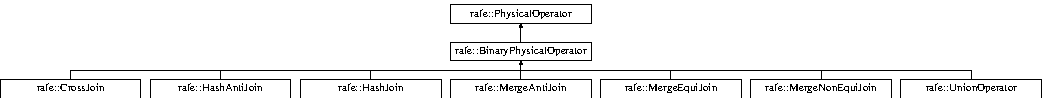
\includegraphics[height=1.297297cm]{classrafe_1_1_binary_physical_operator}
\end{center}
\end{figure}
\subsection*{Public Member Functions}
\begin{DoxyCompactItemize}
\item 
virtual void \hyperlink{classrafe_1_1_binary_physical_operator_a58ce0a14b970b2c932254419877a2e0e}{accept} (\hyperlink{classrafe_1_1_physical_operator_visitor}{Physical\+Operator\+Visitor} \&v)=0
\end{DoxyCompactItemize}
\subsection*{Public Attributes}
\begin{DoxyCompactItemize}
\item 
std\+::shared\+\_\+ptr$<$ \hyperlink{classrafe_1_1_physical_operator}{Physical\+Operator} $>$ \hyperlink{classrafe_1_1_binary_physical_operator_a3ca06613d63ed240f6306f0fb36a5d26}{left\+Child}
\item 
std\+::shared\+\_\+ptr$<$ \hyperlink{classrafe_1_1_physical_operator}{Physical\+Operator} $>$ \hyperlink{classrafe_1_1_binary_physical_operator_a0c90c9b14fd1e543cf721cdb54f658fd}{right\+Child}
\end{DoxyCompactItemize}


\subsection{Detailed Description}
Base class for operators with two inputs. 

\subsection{Member Function Documentation}
\hypertarget{classrafe_1_1_binary_physical_operator_a58ce0a14b970b2c932254419877a2e0e}{\index{rafe\+::\+Binary\+Physical\+Operator@{rafe\+::\+Binary\+Physical\+Operator}!accept@{accept}}
\index{accept@{accept}!rafe\+::\+Binary\+Physical\+Operator@{rafe\+::\+Binary\+Physical\+Operator}}
\subsubsection[{accept}]{\setlength{\rightskip}{0pt plus 5cm}virtual void rafe\+::\+Binary\+Physical\+Operator\+::accept (
\begin{DoxyParamCaption}
\item[{{\bf Physical\+Operator\+Visitor} \&}]{v}
\end{DoxyParamCaption}
)\hspace{0.3cm}{\ttfamily [pure virtual]}}}\label{classrafe_1_1_binary_physical_operator_a58ce0a14b970b2c932254419877a2e0e}
Method for calling visit\mbox{[}node\mbox{]} on given \hyperlink{classrafe_1_1_physical_operator_visitor}{Physical\+Operator\+Visitor}. 
\begin{DoxyParams}{Parameters}
{\em v} & \hyperlink{classrafe_1_1_physical_operator_visitor}{Physical\+Operator\+Visitor}, on which to call function. \\
\hline
\end{DoxyParams}


Implements \hyperlink{classrafe_1_1_physical_operator_a263a89f54604263cea897c5adf8944a3}{rafe\+::\+Physical\+Operator}.



Implemented in \hyperlink{classrafe_1_1_union_operator_a5ae4b5f486376c816b10a81adbe784c7}{rafe\+::\+Union\+Operator}, \hyperlink{classrafe_1_1_merge_anti_join_aae93ebacaaed68ab8af8f38a09cfe8e7}{rafe\+::\+Merge\+Anti\+Join}, \hyperlink{classrafe_1_1_hash_anti_join_a3df56df88dd2e9280d6243cba23b4ac4}{rafe\+::\+Hash\+Anti\+Join}, \hyperlink{classrafe_1_1_hash_join_abd86be090582ddf7e87ac7d3dd2f60a7}{rafe\+::\+Hash\+Join}, \hyperlink{classrafe_1_1_merge_equi_join_a612f15e10eb741126e282b605fef0921}{rafe\+::\+Merge\+Equi\+Join}, \hyperlink{classrafe_1_1_merge_non_equi_join_a3accb9ad7ae5851370152885c23c6048}{rafe\+::\+Merge\+Non\+Equi\+Join}, and \hyperlink{classrafe_1_1_cross_join_a3d9272caf9e1f2394f0d384f2813258a}{rafe\+::\+Cross\+Join}.



\subsection{Member Data Documentation}
\hypertarget{classrafe_1_1_binary_physical_operator_a3ca06613d63ed240f6306f0fb36a5d26}{\index{rafe\+::\+Binary\+Physical\+Operator@{rafe\+::\+Binary\+Physical\+Operator}!left\+Child@{left\+Child}}
\index{left\+Child@{left\+Child}!rafe\+::\+Binary\+Physical\+Operator@{rafe\+::\+Binary\+Physical\+Operator}}
\subsubsection[{left\+Child}]{\setlength{\rightskip}{0pt plus 5cm}std\+::shared\+\_\+ptr$<${\bf Physical\+Operator}$>$ rafe\+::\+Binary\+Physical\+Operator\+::left\+Child}}\label{classrafe_1_1_binary_physical_operator_a3ca06613d63ed240f6306f0fb36a5d26}
Stores left input operator. \hypertarget{classrafe_1_1_binary_physical_operator_a0c90c9b14fd1e543cf721cdb54f658fd}{\index{rafe\+::\+Binary\+Physical\+Operator@{rafe\+::\+Binary\+Physical\+Operator}!right\+Child@{right\+Child}}
\index{right\+Child@{right\+Child}!rafe\+::\+Binary\+Physical\+Operator@{rafe\+::\+Binary\+Physical\+Operator}}
\subsubsection[{right\+Child}]{\setlength{\rightskip}{0pt plus 5cm}std\+::shared\+\_\+ptr$<${\bf Physical\+Operator}$>$ rafe\+::\+Binary\+Physical\+Operator\+::right\+Child}}\label{classrafe_1_1_binary_physical_operator_a0c90c9b14fd1e543cf721cdb54f658fd}
Stores right input operator. 

The documentation for this class was generated from the following file\+:\begin{DoxyCompactItemize}
\item 
C\+:/\+Users/\+Marcel/\+Documents/\+Visual Studio 2012/\+Projects/\+Relational\+Query\+Evaluator/\+Relational\+Query\+Evaluator/Physical\+Operator.\+h\end{DoxyCompactItemize}

\hypertarget{classrafe_1_1_bobox_plan_writing_physical_operator_visitor}{\section{rafe\+:\+:Bobox\+Plan\+Writing\+Physical\+Operator\+Visitor Class Reference}
\label{classrafe_1_1_bobox_plan_writing_physical_operator_visitor}\index{rafe\+::\+Bobox\+Plan\+Writing\+Physical\+Operator\+Visitor@{rafe\+::\+Bobox\+Plan\+Writing\+Physical\+Operator\+Visitor}}
}


{\ttfamily \#include $<$Physical\+Operator\+Visitor.\+h$>$}

Inheritance diagram for rafe\+:\+:Bobox\+Plan\+Writing\+Physical\+Operator\+Visitor\+:\begin{figure}[H]
\begin{center}
\leavevmode
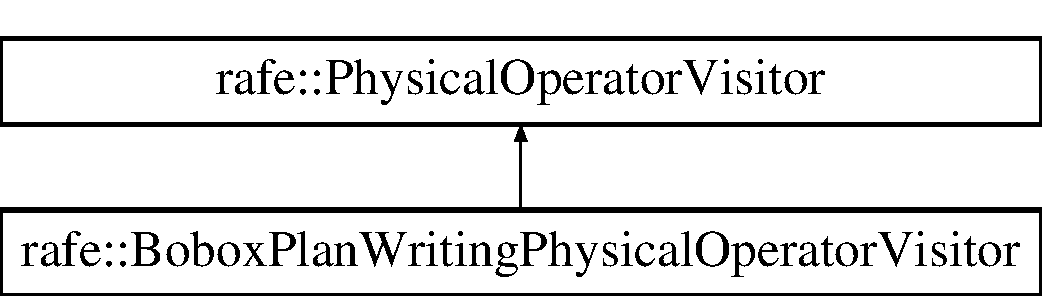
\includegraphics[height=2.000000cm]{classrafe_1_1_bobox_plan_writing_physical_operator_visitor}
\end{center}
\end{figure}
\subsection*{Public Member Functions}
\begin{DoxyCompactItemize}
\item 
\hyperlink{classrafe_1_1_bobox_plan_writing_physical_operator_visitor_afa5e686be89010277091a1d2f1f06dc2}{Bobox\+Plan\+Writing\+Physical\+Operator\+Visitor} ()
\item 
std\+::string \hyperlink{classrafe_1_1_bobox_plan_writing_physical_operator_visitor_ae1b065e58edaf26fa63ce0ad6e7d4acd}{write\+Plan} (std\+::shared\+\_\+ptr$<$ \hyperlink{classrafe_1_1_physical_operator}{Physical\+Operator} $>$ \&plan)
\item 
void \hyperlink{classrafe_1_1_bobox_plan_writing_physical_operator_visitor_a729ee192bceef48ed5221447427be2a4}{visit\+Filter} (\hyperlink{classrafe_1_1_filter}{Filter} $\ast$node)
\item 
void \hyperlink{classrafe_1_1_bobox_plan_writing_physical_operator_visitor_a34f3d494a32fdc1e694ea4568f09db28}{visit\+Filter\+Keeping\+Order} (\hyperlink{classrafe_1_1_filter_keeping_order}{Filter\+Keeping\+Order} $\ast$node)
\item 
void \hyperlink{classrafe_1_1_bobox_plan_writing_physical_operator_visitor_a63be13a7222bfdb4a317334b0b2f892d}{visit\+Sort\+Operator} (\hyperlink{classrafe_1_1_sort_operator}{Sort\+Operator} $\ast$node)
\item 
void \hyperlink{classrafe_1_1_bobox_plan_writing_physical_operator_visitor_a424e82f02063f08ec2849a4728f49b83}{visit\+Merge\+Equi\+Join} (\hyperlink{classrafe_1_1_merge_equi_join}{Merge\+Equi\+Join} $\ast$node)
\item 
void \hyperlink{classrafe_1_1_bobox_plan_writing_physical_operator_visitor_af9342d338c7b1f83e4c6bb2250915adc}{visit\+Merge\+Non\+Equi\+Join} (\hyperlink{classrafe_1_1_merge_non_equi_join}{Merge\+Non\+Equi\+Join} $\ast$node)
\item 
void \hyperlink{classrafe_1_1_bobox_plan_writing_physical_operator_visitor_af8ff4c17855ea7872ed2871aa317591d}{visit\+Cross\+Join} (\hyperlink{classrafe_1_1_cross_join}{Cross\+Join} $\ast$node)
\item 
void \hyperlink{classrafe_1_1_bobox_plan_writing_physical_operator_visitor_ad0924de22102447e0e6c38a90432f3c6}{visit\+Hash\+Join} (\hyperlink{classrafe_1_1_hash_join}{Hash\+Join} $\ast$node)
\item 
void \hyperlink{classrafe_1_1_bobox_plan_writing_physical_operator_visitor_a4c75cb58ec95bc07e9923a3b7c0c2175}{visit\+Hash\+Anti\+Join} (\hyperlink{classrafe_1_1_hash_anti_join}{Hash\+Anti\+Join} $\ast$node)
\item 
void \hyperlink{classrafe_1_1_bobox_plan_writing_physical_operator_visitor_a44f741c5e3ad55bdb934641371057000}{visit\+Merge\+Anti\+Join} (\hyperlink{classrafe_1_1_merge_anti_join}{Merge\+Anti\+Join} $\ast$node)
\item 
void \hyperlink{classrafe_1_1_bobox_plan_writing_physical_operator_visitor_a20fc58d77f1fba7b536bd8c0920641c5}{visit\+Union\+Operator} (\hyperlink{classrafe_1_1_union_operator}{Union\+Operator} $\ast$node)
\item 
void \hyperlink{classrafe_1_1_bobox_plan_writing_physical_operator_visitor_a8f9890744b4a3a64e1d574d4d12bc1ca}{visit\+Hash\+Group} (\hyperlink{classrafe_1_1_hash_group}{Hash\+Group} $\ast$node)
\item 
void \hyperlink{classrafe_1_1_bobox_plan_writing_physical_operator_visitor_ab0f53218eefa3103840afe5bf7fcf9ab}{visit\+Sorted\+Group} (\hyperlink{classrafe_1_1_sorted_group}{Sorted\+Group} $\ast$node)
\item 
void \hyperlink{classrafe_1_1_bobox_plan_writing_physical_operator_visitor_a38591cef68b9a97fc8e854827d33103b}{visit\+Columns\+Operations\+Operator} (\hyperlink{classrafe_1_1_columns_operations_operator}{Columns\+Operations\+Operator} $\ast$node)
\item 
void \hyperlink{classrafe_1_1_bobox_plan_writing_physical_operator_visitor_a747d8a89471bcf19b29d4eb8f9be5196}{visit\+Scan\+And\+Sort\+By\+Index} (\hyperlink{classrafe_1_1_scan_and_sort_by_index}{Scan\+And\+Sort\+By\+Index} $\ast$node)
\item 
void \hyperlink{classrafe_1_1_bobox_plan_writing_physical_operator_visitor_ab7918b1aa4d801ec86d42b3cbb6d0fe1}{visit\+Table\+Scan} (\hyperlink{classrafe_1_1_table_scan}{Table\+Scan} $\ast$node)
\item 
void \hyperlink{classrafe_1_1_bobox_plan_writing_physical_operator_visitor_a600bfeaec99ab68049069543bad70908}{visit\+Index\+Scan} (\hyperlink{classrafe_1_1_index_scan}{Index\+Scan} $\ast$node)
\end{DoxyCompactItemize}


\subsection{Detailed Description}
Generates bobox string output. 

\subsection{Constructor \& Destructor Documentation}
\hypertarget{classrafe_1_1_bobox_plan_writing_physical_operator_visitor_afa5e686be89010277091a1d2f1f06dc2}{\index{rafe\+::\+Bobox\+Plan\+Writing\+Physical\+Operator\+Visitor@{rafe\+::\+Bobox\+Plan\+Writing\+Physical\+Operator\+Visitor}!Bobox\+Plan\+Writing\+Physical\+Operator\+Visitor@{Bobox\+Plan\+Writing\+Physical\+Operator\+Visitor}}
\index{Bobox\+Plan\+Writing\+Physical\+Operator\+Visitor@{Bobox\+Plan\+Writing\+Physical\+Operator\+Visitor}!rafe\+::\+Bobox\+Plan\+Writing\+Physical\+Operator\+Visitor@{rafe\+::\+Bobox\+Plan\+Writing\+Physical\+Operator\+Visitor}}
\subsubsection[{Bobox\+Plan\+Writing\+Physical\+Operator\+Visitor}]{\setlength{\rightskip}{0pt plus 5cm}rafe\+::\+Bobox\+Plan\+Writing\+Physical\+Operator\+Visitor\+::\+Bobox\+Plan\+Writing\+Physical\+Operator\+Visitor (
\begin{DoxyParamCaption}
{}
\end{DoxyParamCaption}
)}}\label{classrafe_1_1_bobox_plan_writing_physical_operator_visitor_afa5e686be89010277091a1d2f1f06dc2}
Creates new instace of \hyperlink{classrafe_1_1_bobox_plan_writing_physical_operator_visitor}{Bobox\+Plan\+Writing\+Physical\+Operator\+Visitor}. 

\subsection{Member Function Documentation}
\hypertarget{classrafe_1_1_bobox_plan_writing_physical_operator_visitor_a38591cef68b9a97fc8e854827d33103b}{\index{rafe\+::\+Bobox\+Plan\+Writing\+Physical\+Operator\+Visitor@{rafe\+::\+Bobox\+Plan\+Writing\+Physical\+Operator\+Visitor}!visit\+Columns\+Operations\+Operator@{visit\+Columns\+Operations\+Operator}}
\index{visit\+Columns\+Operations\+Operator@{visit\+Columns\+Operations\+Operator}!rafe\+::\+Bobox\+Plan\+Writing\+Physical\+Operator\+Visitor@{rafe\+::\+Bobox\+Plan\+Writing\+Physical\+Operator\+Visitor}}
\subsubsection[{visit\+Columns\+Operations\+Operator}]{\setlength{\rightskip}{0pt plus 5cm}void rafe\+::\+Bobox\+Plan\+Writing\+Physical\+Operator\+Visitor\+::visit\+Columns\+Operations\+Operator (
\begin{DoxyParamCaption}
\item[{{\bf Columns\+Operations\+Operator} $\ast$}]{node}
\end{DoxyParamCaption}
)\hspace{0.3cm}{\ttfamily [virtual]}}}\label{classrafe_1_1_bobox_plan_writing_physical_operator_visitor_a38591cef68b9a97fc8e854827d33103b}
Visits physical operator \hyperlink{classrafe_1_1_columns_operations_operator}{Columns\+Operations\+Operator}. 
\begin{DoxyParams}{Parameters}
{\em node} & visited \hyperlink{classrafe_1_1_columns_operations_operator}{Columns\+Operations\+Operator}. \\
\hline
\end{DoxyParams}


Reimplemented from \hyperlink{classrafe_1_1_physical_operator_visitor_ab69b85d7a2c8f89986d84cbcce6f2f89}{rafe\+::\+Physical\+Operator\+Visitor}.

\hypertarget{classrafe_1_1_bobox_plan_writing_physical_operator_visitor_af8ff4c17855ea7872ed2871aa317591d}{\index{rafe\+::\+Bobox\+Plan\+Writing\+Physical\+Operator\+Visitor@{rafe\+::\+Bobox\+Plan\+Writing\+Physical\+Operator\+Visitor}!visit\+Cross\+Join@{visit\+Cross\+Join}}
\index{visit\+Cross\+Join@{visit\+Cross\+Join}!rafe\+::\+Bobox\+Plan\+Writing\+Physical\+Operator\+Visitor@{rafe\+::\+Bobox\+Plan\+Writing\+Physical\+Operator\+Visitor}}
\subsubsection[{visit\+Cross\+Join}]{\setlength{\rightskip}{0pt plus 5cm}void rafe\+::\+Bobox\+Plan\+Writing\+Physical\+Operator\+Visitor\+::visit\+Cross\+Join (
\begin{DoxyParamCaption}
\item[{{\bf Cross\+Join} $\ast$}]{node}
\end{DoxyParamCaption}
)\hspace{0.3cm}{\ttfamily [virtual]}}}\label{classrafe_1_1_bobox_plan_writing_physical_operator_visitor_af8ff4c17855ea7872ed2871aa317591d}
Visits physical operator \hyperlink{classrafe_1_1_cross_join}{Cross\+Join}. 
\begin{DoxyParams}{Parameters}
{\em node} & visited \hyperlink{classrafe_1_1_cross_join}{Cross\+Join}. \\
\hline
\end{DoxyParams}


Reimplemented from \hyperlink{classrafe_1_1_physical_operator_visitor_acc39509ae79aa6848ec928cc4f616d61}{rafe\+::\+Physical\+Operator\+Visitor}.

\hypertarget{classrafe_1_1_bobox_plan_writing_physical_operator_visitor_a729ee192bceef48ed5221447427be2a4}{\index{rafe\+::\+Bobox\+Plan\+Writing\+Physical\+Operator\+Visitor@{rafe\+::\+Bobox\+Plan\+Writing\+Physical\+Operator\+Visitor}!visit\+Filter@{visit\+Filter}}
\index{visit\+Filter@{visit\+Filter}!rafe\+::\+Bobox\+Plan\+Writing\+Physical\+Operator\+Visitor@{rafe\+::\+Bobox\+Plan\+Writing\+Physical\+Operator\+Visitor}}
\subsubsection[{visit\+Filter}]{\setlength{\rightskip}{0pt plus 5cm}void rafe\+::\+Bobox\+Plan\+Writing\+Physical\+Operator\+Visitor\+::visit\+Filter (
\begin{DoxyParamCaption}
\item[{{\bf Filter} $\ast$}]{node}
\end{DoxyParamCaption}
)\hspace{0.3cm}{\ttfamily [virtual]}}}\label{classrafe_1_1_bobox_plan_writing_physical_operator_visitor_a729ee192bceef48ed5221447427be2a4}
Visits physical operator \hyperlink{classrafe_1_1_filter}{Filter}. 
\begin{DoxyParams}{Parameters}
{\em node} & visited \hyperlink{classrafe_1_1_filter}{Filter}. \\
\hline
\end{DoxyParams}


Reimplemented from \hyperlink{classrafe_1_1_physical_operator_visitor_a516a84d305910f3e1b9d1ae2cb184b24}{rafe\+::\+Physical\+Operator\+Visitor}.

\hypertarget{classrafe_1_1_bobox_plan_writing_physical_operator_visitor_a34f3d494a32fdc1e694ea4568f09db28}{\index{rafe\+::\+Bobox\+Plan\+Writing\+Physical\+Operator\+Visitor@{rafe\+::\+Bobox\+Plan\+Writing\+Physical\+Operator\+Visitor}!visit\+Filter\+Keeping\+Order@{visit\+Filter\+Keeping\+Order}}
\index{visit\+Filter\+Keeping\+Order@{visit\+Filter\+Keeping\+Order}!rafe\+::\+Bobox\+Plan\+Writing\+Physical\+Operator\+Visitor@{rafe\+::\+Bobox\+Plan\+Writing\+Physical\+Operator\+Visitor}}
\subsubsection[{visit\+Filter\+Keeping\+Order}]{\setlength{\rightskip}{0pt plus 5cm}void rafe\+::\+Bobox\+Plan\+Writing\+Physical\+Operator\+Visitor\+::visit\+Filter\+Keeping\+Order (
\begin{DoxyParamCaption}
\item[{{\bf Filter\+Keeping\+Order} $\ast$}]{node}
\end{DoxyParamCaption}
)\hspace{0.3cm}{\ttfamily [virtual]}}}\label{classrafe_1_1_bobox_plan_writing_physical_operator_visitor_a34f3d494a32fdc1e694ea4568f09db28}
Visits physical operator \hyperlink{classrafe_1_1_filter_keeping_order}{Filter\+Keeping\+Order}. 
\begin{DoxyParams}{Parameters}
{\em node} & visited \hyperlink{classrafe_1_1_filter_keeping_order}{Filter\+Keeping\+Order}. \\
\hline
\end{DoxyParams}


Reimplemented from \hyperlink{classrafe_1_1_physical_operator_visitor_a7b581054d167c71fa5443570a6808740}{rafe\+::\+Physical\+Operator\+Visitor}.

\hypertarget{classrafe_1_1_bobox_plan_writing_physical_operator_visitor_a4c75cb58ec95bc07e9923a3b7c0c2175}{\index{rafe\+::\+Bobox\+Plan\+Writing\+Physical\+Operator\+Visitor@{rafe\+::\+Bobox\+Plan\+Writing\+Physical\+Operator\+Visitor}!visit\+Hash\+Anti\+Join@{visit\+Hash\+Anti\+Join}}
\index{visit\+Hash\+Anti\+Join@{visit\+Hash\+Anti\+Join}!rafe\+::\+Bobox\+Plan\+Writing\+Physical\+Operator\+Visitor@{rafe\+::\+Bobox\+Plan\+Writing\+Physical\+Operator\+Visitor}}
\subsubsection[{visit\+Hash\+Anti\+Join}]{\setlength{\rightskip}{0pt plus 5cm}void rafe\+::\+Bobox\+Plan\+Writing\+Physical\+Operator\+Visitor\+::visit\+Hash\+Anti\+Join (
\begin{DoxyParamCaption}
\item[{{\bf Hash\+Anti\+Join} $\ast$}]{node}
\end{DoxyParamCaption}
)\hspace{0.3cm}{\ttfamily [virtual]}}}\label{classrafe_1_1_bobox_plan_writing_physical_operator_visitor_a4c75cb58ec95bc07e9923a3b7c0c2175}
Visits physical operator \hyperlink{classrafe_1_1_hash_anti_join}{Hash\+Anti\+Join}. 
\begin{DoxyParams}{Parameters}
{\em node} & visited \hyperlink{classrafe_1_1_hash_anti_join}{Hash\+Anti\+Join}. \\
\hline
\end{DoxyParams}


Reimplemented from \hyperlink{classrafe_1_1_physical_operator_visitor_a9415b5939da4948ac922e63fbece1135}{rafe\+::\+Physical\+Operator\+Visitor}.

\hypertarget{classrafe_1_1_bobox_plan_writing_physical_operator_visitor_a8f9890744b4a3a64e1d574d4d12bc1ca}{\index{rafe\+::\+Bobox\+Plan\+Writing\+Physical\+Operator\+Visitor@{rafe\+::\+Bobox\+Plan\+Writing\+Physical\+Operator\+Visitor}!visit\+Hash\+Group@{visit\+Hash\+Group}}
\index{visit\+Hash\+Group@{visit\+Hash\+Group}!rafe\+::\+Bobox\+Plan\+Writing\+Physical\+Operator\+Visitor@{rafe\+::\+Bobox\+Plan\+Writing\+Physical\+Operator\+Visitor}}
\subsubsection[{visit\+Hash\+Group}]{\setlength{\rightskip}{0pt plus 5cm}void rafe\+::\+Bobox\+Plan\+Writing\+Physical\+Operator\+Visitor\+::visit\+Hash\+Group (
\begin{DoxyParamCaption}
\item[{{\bf Hash\+Group} $\ast$}]{node}
\end{DoxyParamCaption}
)\hspace{0.3cm}{\ttfamily [virtual]}}}\label{classrafe_1_1_bobox_plan_writing_physical_operator_visitor_a8f9890744b4a3a64e1d574d4d12bc1ca}
Visits physical operator \hyperlink{classrafe_1_1_hash_group}{Hash\+Group}. 
\begin{DoxyParams}{Parameters}
{\em node} & visited \hyperlink{classrafe_1_1_hash_group}{Hash\+Group}. \\
\hline
\end{DoxyParams}


Reimplemented from \hyperlink{classrafe_1_1_physical_operator_visitor_ab6a2b2b02f2237fd41e6c44f5b2ede9b}{rafe\+::\+Physical\+Operator\+Visitor}.

\hypertarget{classrafe_1_1_bobox_plan_writing_physical_operator_visitor_ad0924de22102447e0e6c38a90432f3c6}{\index{rafe\+::\+Bobox\+Plan\+Writing\+Physical\+Operator\+Visitor@{rafe\+::\+Bobox\+Plan\+Writing\+Physical\+Operator\+Visitor}!visit\+Hash\+Join@{visit\+Hash\+Join}}
\index{visit\+Hash\+Join@{visit\+Hash\+Join}!rafe\+::\+Bobox\+Plan\+Writing\+Physical\+Operator\+Visitor@{rafe\+::\+Bobox\+Plan\+Writing\+Physical\+Operator\+Visitor}}
\subsubsection[{visit\+Hash\+Join}]{\setlength{\rightskip}{0pt plus 5cm}void rafe\+::\+Bobox\+Plan\+Writing\+Physical\+Operator\+Visitor\+::visit\+Hash\+Join (
\begin{DoxyParamCaption}
\item[{{\bf Hash\+Join} $\ast$}]{node}
\end{DoxyParamCaption}
)\hspace{0.3cm}{\ttfamily [virtual]}}}\label{classrafe_1_1_bobox_plan_writing_physical_operator_visitor_ad0924de22102447e0e6c38a90432f3c6}
Visits physical operator \hyperlink{classrafe_1_1_hash_join}{Hash\+Join}. 
\begin{DoxyParams}{Parameters}
{\em node} & visited \hyperlink{classrafe_1_1_hash_join}{Hash\+Join}. \\
\hline
\end{DoxyParams}


Reimplemented from \hyperlink{classrafe_1_1_physical_operator_visitor_ae36c9ef817768f134d35fe5b3834855c}{rafe\+::\+Physical\+Operator\+Visitor}.

\hypertarget{classrafe_1_1_bobox_plan_writing_physical_operator_visitor_a600bfeaec99ab68049069543bad70908}{\index{rafe\+::\+Bobox\+Plan\+Writing\+Physical\+Operator\+Visitor@{rafe\+::\+Bobox\+Plan\+Writing\+Physical\+Operator\+Visitor}!visit\+Index\+Scan@{visit\+Index\+Scan}}
\index{visit\+Index\+Scan@{visit\+Index\+Scan}!rafe\+::\+Bobox\+Plan\+Writing\+Physical\+Operator\+Visitor@{rafe\+::\+Bobox\+Plan\+Writing\+Physical\+Operator\+Visitor}}
\subsubsection[{visit\+Index\+Scan}]{\setlength{\rightskip}{0pt plus 5cm}void rafe\+::\+Bobox\+Plan\+Writing\+Physical\+Operator\+Visitor\+::visit\+Index\+Scan (
\begin{DoxyParamCaption}
\item[{{\bf Index\+Scan} $\ast$}]{node}
\end{DoxyParamCaption}
)\hspace{0.3cm}{\ttfamily [virtual]}}}\label{classrafe_1_1_bobox_plan_writing_physical_operator_visitor_a600bfeaec99ab68049069543bad70908}
Visits physical operator \hyperlink{classrafe_1_1_index_scan}{Index\+Scan}. 
\begin{DoxyParams}{Parameters}
{\em node} & visited \hyperlink{classrafe_1_1_index_scan}{Index\+Scan}. \\
\hline
\end{DoxyParams}


Reimplemented from \hyperlink{classrafe_1_1_physical_operator_visitor_ac33ea100cdb3e642a58a82c4367de3fd}{rafe\+::\+Physical\+Operator\+Visitor}.

\hypertarget{classrafe_1_1_bobox_plan_writing_physical_operator_visitor_a44f741c5e3ad55bdb934641371057000}{\index{rafe\+::\+Bobox\+Plan\+Writing\+Physical\+Operator\+Visitor@{rafe\+::\+Bobox\+Plan\+Writing\+Physical\+Operator\+Visitor}!visit\+Merge\+Anti\+Join@{visit\+Merge\+Anti\+Join}}
\index{visit\+Merge\+Anti\+Join@{visit\+Merge\+Anti\+Join}!rafe\+::\+Bobox\+Plan\+Writing\+Physical\+Operator\+Visitor@{rafe\+::\+Bobox\+Plan\+Writing\+Physical\+Operator\+Visitor}}
\subsubsection[{visit\+Merge\+Anti\+Join}]{\setlength{\rightskip}{0pt plus 5cm}void rafe\+::\+Bobox\+Plan\+Writing\+Physical\+Operator\+Visitor\+::visit\+Merge\+Anti\+Join (
\begin{DoxyParamCaption}
\item[{{\bf Merge\+Anti\+Join} $\ast$}]{node}
\end{DoxyParamCaption}
)\hspace{0.3cm}{\ttfamily [virtual]}}}\label{classrafe_1_1_bobox_plan_writing_physical_operator_visitor_a44f741c5e3ad55bdb934641371057000}
Visits physical operator \hyperlink{classrafe_1_1_merge_anti_join}{Merge\+Anti\+Join}. 
\begin{DoxyParams}{Parameters}
{\em node} & visited \hyperlink{classrafe_1_1_merge_anti_join}{Merge\+Anti\+Join}. \\
\hline
\end{DoxyParams}


Reimplemented from \hyperlink{classrafe_1_1_physical_operator_visitor_a0f3496aaac992756bbb8f18c1000ed75}{rafe\+::\+Physical\+Operator\+Visitor}.

\hypertarget{classrafe_1_1_bobox_plan_writing_physical_operator_visitor_a424e82f02063f08ec2849a4728f49b83}{\index{rafe\+::\+Bobox\+Plan\+Writing\+Physical\+Operator\+Visitor@{rafe\+::\+Bobox\+Plan\+Writing\+Physical\+Operator\+Visitor}!visit\+Merge\+Equi\+Join@{visit\+Merge\+Equi\+Join}}
\index{visit\+Merge\+Equi\+Join@{visit\+Merge\+Equi\+Join}!rafe\+::\+Bobox\+Plan\+Writing\+Physical\+Operator\+Visitor@{rafe\+::\+Bobox\+Plan\+Writing\+Physical\+Operator\+Visitor}}
\subsubsection[{visit\+Merge\+Equi\+Join}]{\setlength{\rightskip}{0pt plus 5cm}void rafe\+::\+Bobox\+Plan\+Writing\+Physical\+Operator\+Visitor\+::visit\+Merge\+Equi\+Join (
\begin{DoxyParamCaption}
\item[{{\bf Merge\+Equi\+Join} $\ast$}]{node}
\end{DoxyParamCaption}
)\hspace{0.3cm}{\ttfamily [virtual]}}}\label{classrafe_1_1_bobox_plan_writing_physical_operator_visitor_a424e82f02063f08ec2849a4728f49b83}
Visits physical operator \hyperlink{classrafe_1_1_merge_equi_join}{Merge\+Equi\+Join}. 
\begin{DoxyParams}{Parameters}
{\em node} & visited \hyperlink{classrafe_1_1_merge_equi_join}{Merge\+Equi\+Join}. \\
\hline
\end{DoxyParams}


Reimplemented from \hyperlink{classrafe_1_1_physical_operator_visitor_a9fd16981e6fbb9b545b7edeaabcf97bf}{rafe\+::\+Physical\+Operator\+Visitor}.

\hypertarget{classrafe_1_1_bobox_plan_writing_physical_operator_visitor_af9342d338c7b1f83e4c6bb2250915adc}{\index{rafe\+::\+Bobox\+Plan\+Writing\+Physical\+Operator\+Visitor@{rafe\+::\+Bobox\+Plan\+Writing\+Physical\+Operator\+Visitor}!visit\+Merge\+Non\+Equi\+Join@{visit\+Merge\+Non\+Equi\+Join}}
\index{visit\+Merge\+Non\+Equi\+Join@{visit\+Merge\+Non\+Equi\+Join}!rafe\+::\+Bobox\+Plan\+Writing\+Physical\+Operator\+Visitor@{rafe\+::\+Bobox\+Plan\+Writing\+Physical\+Operator\+Visitor}}
\subsubsection[{visit\+Merge\+Non\+Equi\+Join}]{\setlength{\rightskip}{0pt plus 5cm}void rafe\+::\+Bobox\+Plan\+Writing\+Physical\+Operator\+Visitor\+::visit\+Merge\+Non\+Equi\+Join (
\begin{DoxyParamCaption}
\item[{{\bf Merge\+Non\+Equi\+Join} $\ast$}]{node}
\end{DoxyParamCaption}
)\hspace{0.3cm}{\ttfamily [virtual]}}}\label{classrafe_1_1_bobox_plan_writing_physical_operator_visitor_af9342d338c7b1f83e4c6bb2250915adc}
Visits physical operator \hyperlink{classrafe_1_1_merge_non_equi_join}{Merge\+Non\+Equi\+Join}. 
\begin{DoxyParams}{Parameters}
{\em node} & visited \hyperlink{classrafe_1_1_merge_non_equi_join}{Merge\+Non\+Equi\+Join}. \\
\hline
\end{DoxyParams}


Reimplemented from \hyperlink{classrafe_1_1_physical_operator_visitor_a1d4af9c73ece300d7a90c65481cd8e06}{rafe\+::\+Physical\+Operator\+Visitor}.

\hypertarget{classrafe_1_1_bobox_plan_writing_physical_operator_visitor_a747d8a89471bcf19b29d4eb8f9be5196}{\index{rafe\+::\+Bobox\+Plan\+Writing\+Physical\+Operator\+Visitor@{rafe\+::\+Bobox\+Plan\+Writing\+Physical\+Operator\+Visitor}!visit\+Scan\+And\+Sort\+By\+Index@{visit\+Scan\+And\+Sort\+By\+Index}}
\index{visit\+Scan\+And\+Sort\+By\+Index@{visit\+Scan\+And\+Sort\+By\+Index}!rafe\+::\+Bobox\+Plan\+Writing\+Physical\+Operator\+Visitor@{rafe\+::\+Bobox\+Plan\+Writing\+Physical\+Operator\+Visitor}}
\subsubsection[{visit\+Scan\+And\+Sort\+By\+Index}]{\setlength{\rightskip}{0pt plus 5cm}void rafe\+::\+Bobox\+Plan\+Writing\+Physical\+Operator\+Visitor\+::visit\+Scan\+And\+Sort\+By\+Index (
\begin{DoxyParamCaption}
\item[{{\bf Scan\+And\+Sort\+By\+Index} $\ast$}]{node}
\end{DoxyParamCaption}
)\hspace{0.3cm}{\ttfamily [virtual]}}}\label{classrafe_1_1_bobox_plan_writing_physical_operator_visitor_a747d8a89471bcf19b29d4eb8f9be5196}
Visits physical operator \hyperlink{classrafe_1_1_scan_and_sort_by_index}{Scan\+And\+Sort\+By\+Index}. 
\begin{DoxyParams}{Parameters}
{\em node} & visited \hyperlink{classrafe_1_1_scan_and_sort_by_index}{Scan\+And\+Sort\+By\+Index}. \\
\hline
\end{DoxyParams}


Reimplemented from \hyperlink{classrafe_1_1_physical_operator_visitor_a4f8cbef9d1c5a58fceb44deb4a7d998c}{rafe\+::\+Physical\+Operator\+Visitor}.

\hypertarget{classrafe_1_1_bobox_plan_writing_physical_operator_visitor_ab0f53218eefa3103840afe5bf7fcf9ab}{\index{rafe\+::\+Bobox\+Plan\+Writing\+Physical\+Operator\+Visitor@{rafe\+::\+Bobox\+Plan\+Writing\+Physical\+Operator\+Visitor}!visit\+Sorted\+Group@{visit\+Sorted\+Group}}
\index{visit\+Sorted\+Group@{visit\+Sorted\+Group}!rafe\+::\+Bobox\+Plan\+Writing\+Physical\+Operator\+Visitor@{rafe\+::\+Bobox\+Plan\+Writing\+Physical\+Operator\+Visitor}}
\subsubsection[{visit\+Sorted\+Group}]{\setlength{\rightskip}{0pt plus 5cm}void rafe\+::\+Bobox\+Plan\+Writing\+Physical\+Operator\+Visitor\+::visit\+Sorted\+Group (
\begin{DoxyParamCaption}
\item[{{\bf Sorted\+Group} $\ast$}]{node}
\end{DoxyParamCaption}
)\hspace{0.3cm}{\ttfamily [virtual]}}}\label{classrafe_1_1_bobox_plan_writing_physical_operator_visitor_ab0f53218eefa3103840afe5bf7fcf9ab}
Visits physical operator \hyperlink{classrafe_1_1_sorted_group}{Sorted\+Group}. 
\begin{DoxyParams}{Parameters}
{\em node} & visited \hyperlink{classrafe_1_1_sorted_group}{Sorted\+Group}. \\
\hline
\end{DoxyParams}


Reimplemented from \hyperlink{classrafe_1_1_physical_operator_visitor_afb1b6786bf12f12e3b1c2895bf77e874}{rafe\+::\+Physical\+Operator\+Visitor}.

\hypertarget{classrafe_1_1_bobox_plan_writing_physical_operator_visitor_a63be13a7222bfdb4a317334b0b2f892d}{\index{rafe\+::\+Bobox\+Plan\+Writing\+Physical\+Operator\+Visitor@{rafe\+::\+Bobox\+Plan\+Writing\+Physical\+Operator\+Visitor}!visit\+Sort\+Operator@{visit\+Sort\+Operator}}
\index{visit\+Sort\+Operator@{visit\+Sort\+Operator}!rafe\+::\+Bobox\+Plan\+Writing\+Physical\+Operator\+Visitor@{rafe\+::\+Bobox\+Plan\+Writing\+Physical\+Operator\+Visitor}}
\subsubsection[{visit\+Sort\+Operator}]{\setlength{\rightskip}{0pt plus 5cm}void rafe\+::\+Bobox\+Plan\+Writing\+Physical\+Operator\+Visitor\+::visit\+Sort\+Operator (
\begin{DoxyParamCaption}
\item[{{\bf Sort\+Operator} $\ast$}]{node}
\end{DoxyParamCaption}
)\hspace{0.3cm}{\ttfamily [virtual]}}}\label{classrafe_1_1_bobox_plan_writing_physical_operator_visitor_a63be13a7222bfdb4a317334b0b2f892d}
Visits physical operator \hyperlink{classrafe_1_1_sort_operator}{Sort\+Operator}. 
\begin{DoxyParams}{Parameters}
{\em node} & visited \hyperlink{classrafe_1_1_sort_operator}{Sort\+Operator}. \\
\hline
\end{DoxyParams}


Reimplemented from \hyperlink{classrafe_1_1_physical_operator_visitor_adaee48b1ef175226c860c7b2d70ba15d}{rafe\+::\+Physical\+Operator\+Visitor}.

\hypertarget{classrafe_1_1_bobox_plan_writing_physical_operator_visitor_ab7918b1aa4d801ec86d42b3cbb6d0fe1}{\index{rafe\+::\+Bobox\+Plan\+Writing\+Physical\+Operator\+Visitor@{rafe\+::\+Bobox\+Plan\+Writing\+Physical\+Operator\+Visitor}!visit\+Table\+Scan@{visit\+Table\+Scan}}
\index{visit\+Table\+Scan@{visit\+Table\+Scan}!rafe\+::\+Bobox\+Plan\+Writing\+Physical\+Operator\+Visitor@{rafe\+::\+Bobox\+Plan\+Writing\+Physical\+Operator\+Visitor}}
\subsubsection[{visit\+Table\+Scan}]{\setlength{\rightskip}{0pt plus 5cm}void rafe\+::\+Bobox\+Plan\+Writing\+Physical\+Operator\+Visitor\+::visit\+Table\+Scan (
\begin{DoxyParamCaption}
\item[{{\bf Table\+Scan} $\ast$}]{node}
\end{DoxyParamCaption}
)\hspace{0.3cm}{\ttfamily [virtual]}}}\label{classrafe_1_1_bobox_plan_writing_physical_operator_visitor_ab7918b1aa4d801ec86d42b3cbb6d0fe1}
Visits physical operator \hyperlink{classrafe_1_1_table_scan}{Table\+Scan}. 
\begin{DoxyParams}{Parameters}
{\em node} & visited \hyperlink{classrafe_1_1_table_scan}{Table\+Scan}. \\
\hline
\end{DoxyParams}


Reimplemented from \hyperlink{classrafe_1_1_physical_operator_visitor_ae3d5b2b56e9465713c5ecd4e5fcea9c9}{rafe\+::\+Physical\+Operator\+Visitor}.

\hypertarget{classrafe_1_1_bobox_plan_writing_physical_operator_visitor_a20fc58d77f1fba7b536bd8c0920641c5}{\index{rafe\+::\+Bobox\+Plan\+Writing\+Physical\+Operator\+Visitor@{rafe\+::\+Bobox\+Plan\+Writing\+Physical\+Operator\+Visitor}!visit\+Union\+Operator@{visit\+Union\+Operator}}
\index{visit\+Union\+Operator@{visit\+Union\+Operator}!rafe\+::\+Bobox\+Plan\+Writing\+Physical\+Operator\+Visitor@{rafe\+::\+Bobox\+Plan\+Writing\+Physical\+Operator\+Visitor}}
\subsubsection[{visit\+Union\+Operator}]{\setlength{\rightskip}{0pt plus 5cm}void rafe\+::\+Bobox\+Plan\+Writing\+Physical\+Operator\+Visitor\+::visit\+Union\+Operator (
\begin{DoxyParamCaption}
\item[{{\bf Union\+Operator} $\ast$}]{node}
\end{DoxyParamCaption}
)\hspace{0.3cm}{\ttfamily [virtual]}}}\label{classrafe_1_1_bobox_plan_writing_physical_operator_visitor_a20fc58d77f1fba7b536bd8c0920641c5}
Visits physical operator \hyperlink{classrafe_1_1_union_operator}{Union\+Operator}. 
\begin{DoxyParams}{Parameters}
{\em node} & visited \hyperlink{classrafe_1_1_union_operator}{Union\+Operator}. \\
\hline
\end{DoxyParams}


Reimplemented from \hyperlink{classrafe_1_1_physical_operator_visitor_a01eb10e07cc1fbe7622bc1eb01fa3b79}{rafe\+::\+Physical\+Operator\+Visitor}.

\hypertarget{classrafe_1_1_bobox_plan_writing_physical_operator_visitor_ae1b065e58edaf26fa63ce0ad6e7d4acd}{\index{rafe\+::\+Bobox\+Plan\+Writing\+Physical\+Operator\+Visitor@{rafe\+::\+Bobox\+Plan\+Writing\+Physical\+Operator\+Visitor}!write\+Plan@{write\+Plan}}
\index{write\+Plan@{write\+Plan}!rafe\+::\+Bobox\+Plan\+Writing\+Physical\+Operator\+Visitor@{rafe\+::\+Bobox\+Plan\+Writing\+Physical\+Operator\+Visitor}}
\subsubsection[{write\+Plan}]{\setlength{\rightskip}{0pt plus 5cm}string rafe\+::\+Bobox\+Plan\+Writing\+Physical\+Operator\+Visitor\+::write\+Plan (
\begin{DoxyParamCaption}
\item[{std\+::shared\+\_\+ptr$<$ {\bf Physical\+Operator} $>$ \&}]{plan}
\end{DoxyParamCaption}
)}}\label{classrafe_1_1_bobox_plan_writing_physical_operator_visitor_ae1b065e58edaf26fa63ce0ad6e7d4acd}
Generates bobox output of physical plan. 
\begin{DoxyParams}{Parameters}
{\em plan} & -\/ plan to write \\
\hline
\end{DoxyParams}
\begin{DoxyReturn}{Returns}
bobox plan representation 
\end{DoxyReturn}


The documentation for this class was generated from the following files\+:\begin{DoxyCompactItemize}
\item 
C\+:/\+Users/\+Marcel/\+Documents/\+Visual Studio 2012/\+Projects/\+Relational\+Query\+Evaluator/\+Relational\+Query\+Evaluator/Physical\+Operator\+Visitor.\+h\item 
C\+:/\+Users/\+Marcel/\+Documents/\+Visual Studio 2012/\+Projects/\+Relational\+Query\+Evaluator/\+Relational\+Query\+Evaluator/Bobox\+Output.\+cpp\end{DoxyCompactItemize}

\hypertarget{classrafe_1_1_bobox_writing_expression_visitor}{\section{rafe\+:\+:Bobox\+Writing\+Expression\+Visitor Class Reference}
\label{classrafe_1_1_bobox_writing_expression_visitor}\index{rafe\+::\+Bobox\+Writing\+Expression\+Visitor@{rafe\+::\+Bobox\+Writing\+Expression\+Visitor}}
}


{\ttfamily \#include $<$Expression\+Visitors.\+h$>$}

Inheritance diagram for rafe\+:\+:Bobox\+Writing\+Expression\+Visitor\+:\begin{figure}[H]
\begin{center}
\leavevmode
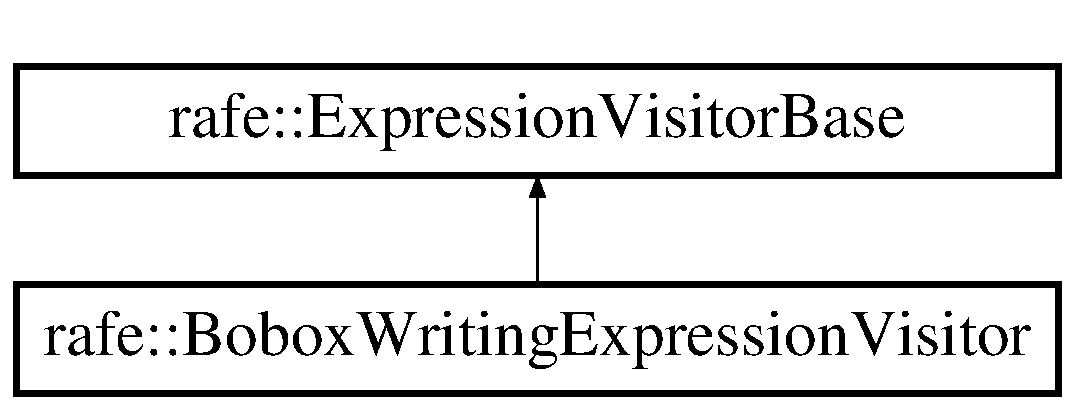
\includegraphics[height=2.000000cm]{classrafe_1_1_bobox_writing_expression_visitor}
\end{center}
\end{figure}
\subsection*{Public Member Functions}
\begin{DoxyCompactItemize}
\item 
\hyperlink{classrafe_1_1_bobox_writing_expression_visitor_a212bf9dc5e42e80474f33bc3c2476020}{Bobox\+Writing\+Expression\+Visitor} (std\+::map$<$ int, int $>$ \&\hyperlink{classrafe_1_1_bobox_writing_expression_visitor_af77757b532d04695137bfa1a4e408f5c}{cols})
\item 
void \hyperlink{classrafe_1_1_bobox_writing_expression_visitor_aa2ebbdd925b785deb29d0ee1f326d917}{visit\+Unary\+Expression} (\hyperlink{classrafe_1_1_unary_expression}{Unary\+Expression} $\ast$expression)
\item 
void \hyperlink{classrafe_1_1_bobox_writing_expression_visitor_a4bf6fe93d12d89e40d30ef811442e666}{visit\+Binary\+Expression} (\hyperlink{classrafe_1_1_binary_expression}{Binary\+Expression} $\ast$expression)
\item 
void \hyperlink{classrafe_1_1_bobox_writing_expression_visitor_a4d004f836ea9b45c8a08de32cb72bdb3}{visit\+Nnary\+Expression} (\hyperlink{classrafe_1_1_nnary_expression}{Nnary\+Expression} $\ast$expression)
\item 
void \hyperlink{classrafe_1_1_bobox_writing_expression_visitor_a2228a1d5a64ae2ef765f5360b5eb9a30}{visit\+Constant} (\hyperlink{classrafe_1_1_constant}{Constant} $\ast$expression)
\item 
void \hyperlink{classrafe_1_1_bobox_writing_expression_visitor_a7c431ef8456be3affdb17692b99d8e50}{visit\+Column} (\hyperlink{classrafe_1_1_column}{Column} $\ast$expression)
\item 
void \hyperlink{classrafe_1_1_bobox_writing_expression_visitor_a5c00ebe39e50c4e6ad35f35a1248ef8e}{visit\+Grouped\+Expression} (\hyperlink{classrafe_1_1_grouped_expression}{Grouped\+Expression} $\ast$expression)
\end{DoxyCompactItemize}
\subsection*{Public Attributes}
\begin{DoxyCompactItemize}
\item 
std\+::string \hyperlink{classrafe_1_1_bobox_writing_expression_visitor_ad9c0ae8342d28bd95bdcec73ff55f6d9}{result}
\item 
std\+::map$<$ int, int $>$ $\ast$ \hyperlink{classrafe_1_1_bobox_writing_expression_visitor_af77757b532d04695137bfa1a4e408f5c}{cols}
\end{DoxyCompactItemize}


\subsection{Detailed Description}
Visitor writes expression in infix for bobox output. 

\subsection{Constructor \& Destructor Documentation}
\hypertarget{classrafe_1_1_bobox_writing_expression_visitor_a212bf9dc5e42e80474f33bc3c2476020}{\index{rafe\+::\+Bobox\+Writing\+Expression\+Visitor@{rafe\+::\+Bobox\+Writing\+Expression\+Visitor}!Bobox\+Writing\+Expression\+Visitor@{Bobox\+Writing\+Expression\+Visitor}}
\index{Bobox\+Writing\+Expression\+Visitor@{Bobox\+Writing\+Expression\+Visitor}!rafe\+::\+Bobox\+Writing\+Expression\+Visitor@{rafe\+::\+Bobox\+Writing\+Expression\+Visitor}}
\subsubsection[{Bobox\+Writing\+Expression\+Visitor}]{\setlength{\rightskip}{0pt plus 5cm}rafe\+::\+Bobox\+Writing\+Expression\+Visitor\+::\+Bobox\+Writing\+Expression\+Visitor (
\begin{DoxyParamCaption}
\item[{std\+::map$<$ int, int $>$ \&}]{cols}
\end{DoxyParamCaption}
)}}\label{classrafe_1_1_bobox_writing_expression_visitor_a212bf9dc5e42e80474f33bc3c2476020}
Creates new instance of \hyperlink{classrafe_1_1_bobox_writing_expression_visitor}{Bobox\+Writing\+Expression\+Visitor}. 
\begin{DoxyParams}{Parameters}
{\em cols} & -\/ structure mapping column unique identifier to number of column in processed bobox operator \\
\hline
\end{DoxyParams}


\subsection{Member Function Documentation}
\hypertarget{classrafe_1_1_bobox_writing_expression_visitor_a4bf6fe93d12d89e40d30ef811442e666}{\index{rafe\+::\+Bobox\+Writing\+Expression\+Visitor@{rafe\+::\+Bobox\+Writing\+Expression\+Visitor}!visit\+Binary\+Expression@{visit\+Binary\+Expression}}
\index{visit\+Binary\+Expression@{visit\+Binary\+Expression}!rafe\+::\+Bobox\+Writing\+Expression\+Visitor@{rafe\+::\+Bobox\+Writing\+Expression\+Visitor}}
\subsubsection[{visit\+Binary\+Expression}]{\setlength{\rightskip}{0pt plus 5cm}void rafe\+::\+Bobox\+Writing\+Expression\+Visitor\+::visit\+Binary\+Expression (
\begin{DoxyParamCaption}
\item[{{\bf Binary\+Expression} $\ast$}]{expression}
\end{DoxyParamCaption}
)\hspace{0.3cm}{\ttfamily [virtual]}}}\label{classrafe_1_1_bobox_writing_expression_visitor_a4bf6fe93d12d89e40d30ef811442e666}
Visits \hyperlink{classrafe_1_1_binary_expression}{Binary\+Expression} element. 
\begin{DoxyParams}{Parameters}
{\em expression} & visited \hyperlink{classrafe_1_1_binary_expression}{Binary\+Expression}. \\
\hline
\end{DoxyParams}


Reimplemented from \hyperlink{classrafe_1_1_expression_visitor_base_a63e53276af3a22d3592f34d05ba97014}{rafe\+::\+Expression\+Visitor\+Base}.

\hypertarget{classrafe_1_1_bobox_writing_expression_visitor_a7c431ef8456be3affdb17692b99d8e50}{\index{rafe\+::\+Bobox\+Writing\+Expression\+Visitor@{rafe\+::\+Bobox\+Writing\+Expression\+Visitor}!visit\+Column@{visit\+Column}}
\index{visit\+Column@{visit\+Column}!rafe\+::\+Bobox\+Writing\+Expression\+Visitor@{rafe\+::\+Bobox\+Writing\+Expression\+Visitor}}
\subsubsection[{visit\+Column}]{\setlength{\rightskip}{0pt plus 5cm}void rafe\+::\+Bobox\+Writing\+Expression\+Visitor\+::visit\+Column (
\begin{DoxyParamCaption}
\item[{{\bf Column} $\ast$}]{expression}
\end{DoxyParamCaption}
)\hspace{0.3cm}{\ttfamily [virtual]}}}\label{classrafe_1_1_bobox_writing_expression_visitor_a7c431ef8456be3affdb17692b99d8e50}
Visits \hyperlink{classrafe_1_1_column}{Column} element. 
\begin{DoxyParams}{Parameters}
{\em expression} & visited \hyperlink{classrafe_1_1_column}{Column}. \\
\hline
\end{DoxyParams}


Reimplemented from \hyperlink{classrafe_1_1_expression_visitor_base_a4eaa77bf4105d1cbdde4feb047228255}{rafe\+::\+Expression\+Visitor\+Base}.

\hypertarget{classrafe_1_1_bobox_writing_expression_visitor_a2228a1d5a64ae2ef765f5360b5eb9a30}{\index{rafe\+::\+Bobox\+Writing\+Expression\+Visitor@{rafe\+::\+Bobox\+Writing\+Expression\+Visitor}!visit\+Constant@{visit\+Constant}}
\index{visit\+Constant@{visit\+Constant}!rafe\+::\+Bobox\+Writing\+Expression\+Visitor@{rafe\+::\+Bobox\+Writing\+Expression\+Visitor}}
\subsubsection[{visit\+Constant}]{\setlength{\rightskip}{0pt plus 5cm}void rafe\+::\+Bobox\+Writing\+Expression\+Visitor\+::visit\+Constant (
\begin{DoxyParamCaption}
\item[{{\bf Constant} $\ast$}]{expression}
\end{DoxyParamCaption}
)\hspace{0.3cm}{\ttfamily [virtual]}}}\label{classrafe_1_1_bobox_writing_expression_visitor_a2228a1d5a64ae2ef765f5360b5eb9a30}
Visits \hyperlink{classrafe_1_1_constant}{Constant} element. 
\begin{DoxyParams}{Parameters}
{\em expression} & visited \hyperlink{classrafe_1_1_constant}{Constant}. \\
\hline
\end{DoxyParams}


Reimplemented from \hyperlink{classrafe_1_1_expression_visitor_base_af934111c6881f9f6c3ef3aa51425b9ff}{rafe\+::\+Expression\+Visitor\+Base}.

\hypertarget{classrafe_1_1_bobox_writing_expression_visitor_a5c00ebe39e50c4e6ad35f35a1248ef8e}{\index{rafe\+::\+Bobox\+Writing\+Expression\+Visitor@{rafe\+::\+Bobox\+Writing\+Expression\+Visitor}!visit\+Grouped\+Expression@{visit\+Grouped\+Expression}}
\index{visit\+Grouped\+Expression@{visit\+Grouped\+Expression}!rafe\+::\+Bobox\+Writing\+Expression\+Visitor@{rafe\+::\+Bobox\+Writing\+Expression\+Visitor}}
\subsubsection[{visit\+Grouped\+Expression}]{\setlength{\rightskip}{0pt plus 5cm}void rafe\+::\+Bobox\+Writing\+Expression\+Visitor\+::visit\+Grouped\+Expression (
\begin{DoxyParamCaption}
\item[{{\bf Grouped\+Expression} $\ast$}]{expression}
\end{DoxyParamCaption}
)\hspace{0.3cm}{\ttfamily [virtual]}}}\label{classrafe_1_1_bobox_writing_expression_visitor_a5c00ebe39e50c4e6ad35f35a1248ef8e}
Visits \hyperlink{classrafe_1_1_grouped_expression}{Grouped\+Expression} element. 
\begin{DoxyParams}{Parameters}
{\em expression} & visited \hyperlink{classrafe_1_1_grouped_expression}{Grouped\+Expression}. \\
\hline
\end{DoxyParams}


Reimplemented from \hyperlink{classrafe_1_1_expression_visitor_base_a76226ab9d571ed7eaf80d2ed7153791c}{rafe\+::\+Expression\+Visitor\+Base}.

\hypertarget{classrafe_1_1_bobox_writing_expression_visitor_a4d004f836ea9b45c8a08de32cb72bdb3}{\index{rafe\+::\+Bobox\+Writing\+Expression\+Visitor@{rafe\+::\+Bobox\+Writing\+Expression\+Visitor}!visit\+Nnary\+Expression@{visit\+Nnary\+Expression}}
\index{visit\+Nnary\+Expression@{visit\+Nnary\+Expression}!rafe\+::\+Bobox\+Writing\+Expression\+Visitor@{rafe\+::\+Bobox\+Writing\+Expression\+Visitor}}
\subsubsection[{visit\+Nnary\+Expression}]{\setlength{\rightskip}{0pt plus 5cm}void rafe\+::\+Bobox\+Writing\+Expression\+Visitor\+::visit\+Nnary\+Expression (
\begin{DoxyParamCaption}
\item[{{\bf Nnary\+Expression} $\ast$}]{expression}
\end{DoxyParamCaption}
)\hspace{0.3cm}{\ttfamily [virtual]}}}\label{classrafe_1_1_bobox_writing_expression_visitor_a4d004f836ea9b45c8a08de32cb72bdb3}
Visits \hyperlink{classrafe_1_1_nnary_expression}{Nnary\+Expression} element. 
\begin{DoxyParams}{Parameters}
{\em expression} & visited \hyperlink{classrafe_1_1_nnary_expression}{Nnary\+Expression}. \\
\hline
\end{DoxyParams}


Reimplemented from \hyperlink{classrafe_1_1_expression_visitor_base_a32f89977f780ccb8aabe5afa1fa42d45}{rafe\+::\+Expression\+Visitor\+Base}.

\hypertarget{classrafe_1_1_bobox_writing_expression_visitor_aa2ebbdd925b785deb29d0ee1f326d917}{\index{rafe\+::\+Bobox\+Writing\+Expression\+Visitor@{rafe\+::\+Bobox\+Writing\+Expression\+Visitor}!visit\+Unary\+Expression@{visit\+Unary\+Expression}}
\index{visit\+Unary\+Expression@{visit\+Unary\+Expression}!rafe\+::\+Bobox\+Writing\+Expression\+Visitor@{rafe\+::\+Bobox\+Writing\+Expression\+Visitor}}
\subsubsection[{visit\+Unary\+Expression}]{\setlength{\rightskip}{0pt plus 5cm}void rafe\+::\+Bobox\+Writing\+Expression\+Visitor\+::visit\+Unary\+Expression (
\begin{DoxyParamCaption}
\item[{{\bf Unary\+Expression} $\ast$}]{expression}
\end{DoxyParamCaption}
)\hspace{0.3cm}{\ttfamily [virtual]}}}\label{classrafe_1_1_bobox_writing_expression_visitor_aa2ebbdd925b785deb29d0ee1f326d917}
Visits \hyperlink{classrafe_1_1_unary_expression}{Unary\+Expression} element. 
\begin{DoxyParams}{Parameters}
{\em expression} & visited \hyperlink{classrafe_1_1_unary_expression}{Unary\+Expression}. \\
\hline
\end{DoxyParams}


Reimplemented from \hyperlink{classrafe_1_1_expression_visitor_base_a439348ee979dff26c30707f1ef499e8c}{rafe\+::\+Expression\+Visitor\+Base}.



\subsection{Member Data Documentation}
\hypertarget{classrafe_1_1_bobox_writing_expression_visitor_af77757b532d04695137bfa1a4e408f5c}{\index{rafe\+::\+Bobox\+Writing\+Expression\+Visitor@{rafe\+::\+Bobox\+Writing\+Expression\+Visitor}!cols@{cols}}
\index{cols@{cols}!rafe\+::\+Bobox\+Writing\+Expression\+Visitor@{rafe\+::\+Bobox\+Writing\+Expression\+Visitor}}
\subsubsection[{cols}]{\setlength{\rightskip}{0pt plus 5cm}std\+::map$<$int, int$>$$\ast$ rafe\+::\+Bobox\+Writing\+Expression\+Visitor\+::cols}}\label{classrafe_1_1_bobox_writing_expression_visitor_af77757b532d04695137bfa1a4e408f5c}
Structure mapping column unique identifier to number of column in processed bobox operator. \hypertarget{classrafe_1_1_bobox_writing_expression_visitor_ad9c0ae8342d28bd95bdcec73ff55f6d9}{\index{rafe\+::\+Bobox\+Writing\+Expression\+Visitor@{rafe\+::\+Bobox\+Writing\+Expression\+Visitor}!result@{result}}
\index{result@{result}!rafe\+::\+Bobox\+Writing\+Expression\+Visitor@{rafe\+::\+Bobox\+Writing\+Expression\+Visitor}}
\subsubsection[{result}]{\setlength{\rightskip}{0pt plus 5cm}std\+::string rafe\+::\+Bobox\+Writing\+Expression\+Visitor\+::result}}\label{classrafe_1_1_bobox_writing_expression_visitor_ad9c0ae8342d28bd95bdcec73ff55f6d9}
Stores tree infix representation. 

The documentation for this class was generated from the following files\+:\begin{DoxyCompactItemize}
\item 
C\+:/\+Users/\+Marcel/\+Documents/\+Visual Studio 2012/\+Projects/\+Relational\+Query\+Evaluator/\+Relational\+Query\+Evaluator/Expression\+Visitors.\+h\item 
C\+:/\+Users/\+Marcel/\+Documents/\+Visual Studio 2012/\+Projects/\+Relational\+Query\+Evaluator/\+Relational\+Query\+Evaluator/Bobox\+Output.\+cpp\end{DoxyCompactItemize}

\hypertarget{classrafe_1_1_cloning_expression_visitor}{\section{rafe\+:\+:Cloning\+Expression\+Visitor Class Reference}
\label{classrafe_1_1_cloning_expression_visitor}\index{rafe\+::\+Cloning\+Expression\+Visitor@{rafe\+::\+Cloning\+Expression\+Visitor}}
}


{\ttfamily \#include $<$Expression\+Visitors.\+h$>$}

Inheritance diagram for rafe\+:\+:Cloning\+Expression\+Visitor\+:\begin{figure}[H]
\begin{center}
\leavevmode
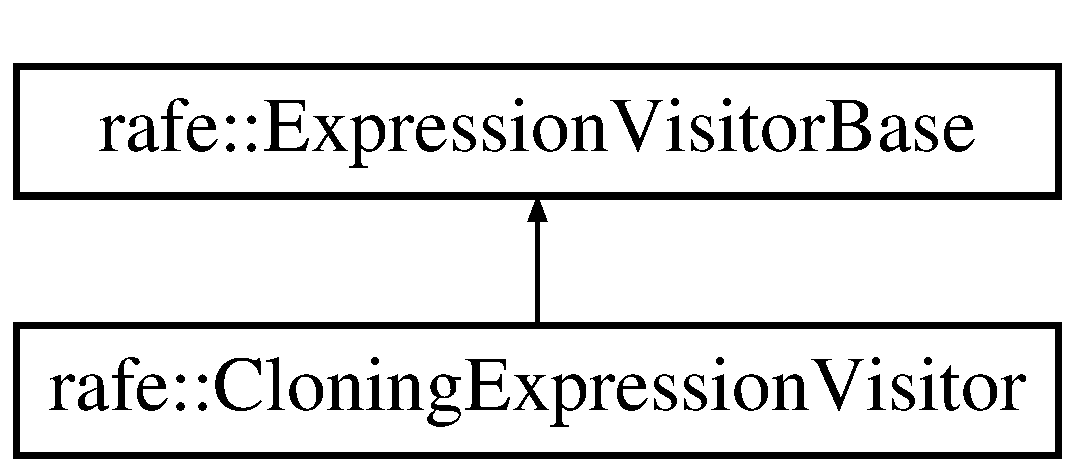
\includegraphics[height=2.000000cm]{classrafe_1_1_cloning_expression_visitor}
\end{center}
\end{figure}
\subsection*{Public Member Functions}
\begin{DoxyCompactItemize}
\item 
void \hyperlink{classrafe_1_1_cloning_expression_visitor_a3b71db5c48bc772a4b8bf52a79ff1e83}{visit\+Unary\+Expression} (\hyperlink{classrafe_1_1_unary_expression}{Unary\+Expression} $\ast$expression)
\item 
void \hyperlink{classrafe_1_1_cloning_expression_visitor_a021e146e191a9fce4b7b82f0c4b4efd4}{visit\+Binary\+Expression} (\hyperlink{classrafe_1_1_binary_expression}{Binary\+Expression} $\ast$expression)
\item 
void \hyperlink{classrafe_1_1_cloning_expression_visitor_ad40e5659edc1098b8465ea64eaeea7cd}{visit\+Nnary\+Expression} (\hyperlink{classrafe_1_1_nnary_expression}{Nnary\+Expression} $\ast$expression)
\item 
void \hyperlink{classrafe_1_1_cloning_expression_visitor_a1fc965624f46b446b7836fc274962f02}{visit\+Constant} (\hyperlink{classrafe_1_1_constant}{Constant} $\ast$expression)
\item 
void \hyperlink{classrafe_1_1_cloning_expression_visitor_a0182fb9588af653201a5450935cf0b87}{visit\+Column} (\hyperlink{classrafe_1_1_column}{Column} $\ast$expression)
\item 
void \hyperlink{classrafe_1_1_cloning_expression_visitor_a54f879bde3c538a907782a32e1eee492}{visit\+Grouped\+Expression} (\hyperlink{classrafe_1_1_grouped_expression}{Grouped\+Expression} $\ast$expression)
\end{DoxyCompactItemize}
\subsection*{Public Attributes}
\begin{DoxyCompactItemize}
\item 
std\+::shared\+\_\+ptr$<$ \hyperlink{classrafe_1_1_expression}{Expression} $>$ \hyperlink{classrafe_1_1_cloning_expression_visitor_a67e902fa64eb5d4bea2c8b7528e6a7e4}{result}
\end{DoxyCompactItemize}


\subsection{Detailed Description}
Visitor maked a copy from visited tree. All nodes are copied. 

\subsection{Member Function Documentation}
\hypertarget{classrafe_1_1_cloning_expression_visitor_a021e146e191a9fce4b7b82f0c4b4efd4}{\index{rafe\+::\+Cloning\+Expression\+Visitor@{rafe\+::\+Cloning\+Expression\+Visitor}!visit\+Binary\+Expression@{visit\+Binary\+Expression}}
\index{visit\+Binary\+Expression@{visit\+Binary\+Expression}!rafe\+::\+Cloning\+Expression\+Visitor@{rafe\+::\+Cloning\+Expression\+Visitor}}
\subsubsection[{visit\+Binary\+Expression}]{\setlength{\rightskip}{0pt plus 5cm}void rafe\+::\+Cloning\+Expression\+Visitor\+::visit\+Binary\+Expression (
\begin{DoxyParamCaption}
\item[{{\bf Binary\+Expression} $\ast$}]{expression}
\end{DoxyParamCaption}
)\hspace{0.3cm}{\ttfamily [virtual]}}}\label{classrafe_1_1_cloning_expression_visitor_a021e146e191a9fce4b7b82f0c4b4efd4}
Visits \hyperlink{classrafe_1_1_binary_expression}{Binary\+Expression} element. 
\begin{DoxyParams}{Parameters}
{\em expression} & visited \hyperlink{classrafe_1_1_binary_expression}{Binary\+Expression}. \\
\hline
\end{DoxyParams}


Reimplemented from \hyperlink{classrafe_1_1_expression_visitor_base_a63e53276af3a22d3592f34d05ba97014}{rafe\+::\+Expression\+Visitor\+Base}.

\hypertarget{classrafe_1_1_cloning_expression_visitor_a0182fb9588af653201a5450935cf0b87}{\index{rafe\+::\+Cloning\+Expression\+Visitor@{rafe\+::\+Cloning\+Expression\+Visitor}!visit\+Column@{visit\+Column}}
\index{visit\+Column@{visit\+Column}!rafe\+::\+Cloning\+Expression\+Visitor@{rafe\+::\+Cloning\+Expression\+Visitor}}
\subsubsection[{visit\+Column}]{\setlength{\rightskip}{0pt plus 5cm}void rafe\+::\+Cloning\+Expression\+Visitor\+::visit\+Column (
\begin{DoxyParamCaption}
\item[{{\bf Column} $\ast$}]{expression}
\end{DoxyParamCaption}
)\hspace{0.3cm}{\ttfamily [virtual]}}}\label{classrafe_1_1_cloning_expression_visitor_a0182fb9588af653201a5450935cf0b87}
Visits \hyperlink{classrafe_1_1_column}{Column} element. 
\begin{DoxyParams}{Parameters}
{\em expression} & visited \hyperlink{classrafe_1_1_column}{Column}. \\
\hline
\end{DoxyParams}


Reimplemented from \hyperlink{classrafe_1_1_expression_visitor_base_a4eaa77bf4105d1cbdde4feb047228255}{rafe\+::\+Expression\+Visitor\+Base}.

\hypertarget{classrafe_1_1_cloning_expression_visitor_a1fc965624f46b446b7836fc274962f02}{\index{rafe\+::\+Cloning\+Expression\+Visitor@{rafe\+::\+Cloning\+Expression\+Visitor}!visit\+Constant@{visit\+Constant}}
\index{visit\+Constant@{visit\+Constant}!rafe\+::\+Cloning\+Expression\+Visitor@{rafe\+::\+Cloning\+Expression\+Visitor}}
\subsubsection[{visit\+Constant}]{\setlength{\rightskip}{0pt plus 5cm}void rafe\+::\+Cloning\+Expression\+Visitor\+::visit\+Constant (
\begin{DoxyParamCaption}
\item[{{\bf Constant} $\ast$}]{expression}
\end{DoxyParamCaption}
)\hspace{0.3cm}{\ttfamily [virtual]}}}\label{classrafe_1_1_cloning_expression_visitor_a1fc965624f46b446b7836fc274962f02}
Visits \hyperlink{classrafe_1_1_constant}{Constant} element. 
\begin{DoxyParams}{Parameters}
{\em expression} & visited \hyperlink{classrafe_1_1_constant}{Constant}. \\
\hline
\end{DoxyParams}


Reimplemented from \hyperlink{classrafe_1_1_expression_visitor_base_af934111c6881f9f6c3ef3aa51425b9ff}{rafe\+::\+Expression\+Visitor\+Base}.

\hypertarget{classrafe_1_1_cloning_expression_visitor_a54f879bde3c538a907782a32e1eee492}{\index{rafe\+::\+Cloning\+Expression\+Visitor@{rafe\+::\+Cloning\+Expression\+Visitor}!visit\+Grouped\+Expression@{visit\+Grouped\+Expression}}
\index{visit\+Grouped\+Expression@{visit\+Grouped\+Expression}!rafe\+::\+Cloning\+Expression\+Visitor@{rafe\+::\+Cloning\+Expression\+Visitor}}
\subsubsection[{visit\+Grouped\+Expression}]{\setlength{\rightskip}{0pt plus 5cm}void rafe\+::\+Cloning\+Expression\+Visitor\+::visit\+Grouped\+Expression (
\begin{DoxyParamCaption}
\item[{{\bf Grouped\+Expression} $\ast$}]{expression}
\end{DoxyParamCaption}
)\hspace{0.3cm}{\ttfamily [virtual]}}}\label{classrafe_1_1_cloning_expression_visitor_a54f879bde3c538a907782a32e1eee492}
Visits \hyperlink{classrafe_1_1_grouped_expression}{Grouped\+Expression} element. 
\begin{DoxyParams}{Parameters}
{\em expression} & visited \hyperlink{classrafe_1_1_grouped_expression}{Grouped\+Expression}. \\
\hline
\end{DoxyParams}


Reimplemented from \hyperlink{classrafe_1_1_expression_visitor_base_a76226ab9d571ed7eaf80d2ed7153791c}{rafe\+::\+Expression\+Visitor\+Base}.

\hypertarget{classrafe_1_1_cloning_expression_visitor_ad40e5659edc1098b8465ea64eaeea7cd}{\index{rafe\+::\+Cloning\+Expression\+Visitor@{rafe\+::\+Cloning\+Expression\+Visitor}!visit\+Nnary\+Expression@{visit\+Nnary\+Expression}}
\index{visit\+Nnary\+Expression@{visit\+Nnary\+Expression}!rafe\+::\+Cloning\+Expression\+Visitor@{rafe\+::\+Cloning\+Expression\+Visitor}}
\subsubsection[{visit\+Nnary\+Expression}]{\setlength{\rightskip}{0pt plus 5cm}void rafe\+::\+Cloning\+Expression\+Visitor\+::visit\+Nnary\+Expression (
\begin{DoxyParamCaption}
\item[{{\bf Nnary\+Expression} $\ast$}]{expression}
\end{DoxyParamCaption}
)\hspace{0.3cm}{\ttfamily [virtual]}}}\label{classrafe_1_1_cloning_expression_visitor_ad40e5659edc1098b8465ea64eaeea7cd}
Visits \hyperlink{classrafe_1_1_nnary_expression}{Nnary\+Expression} element. 
\begin{DoxyParams}{Parameters}
{\em expression} & visited \hyperlink{classrafe_1_1_nnary_expression}{Nnary\+Expression}. \\
\hline
\end{DoxyParams}


Reimplemented from \hyperlink{classrafe_1_1_expression_visitor_base_a32f89977f780ccb8aabe5afa1fa42d45}{rafe\+::\+Expression\+Visitor\+Base}.

\hypertarget{classrafe_1_1_cloning_expression_visitor_a3b71db5c48bc772a4b8bf52a79ff1e83}{\index{rafe\+::\+Cloning\+Expression\+Visitor@{rafe\+::\+Cloning\+Expression\+Visitor}!visit\+Unary\+Expression@{visit\+Unary\+Expression}}
\index{visit\+Unary\+Expression@{visit\+Unary\+Expression}!rafe\+::\+Cloning\+Expression\+Visitor@{rafe\+::\+Cloning\+Expression\+Visitor}}
\subsubsection[{visit\+Unary\+Expression}]{\setlength{\rightskip}{0pt plus 5cm}void rafe\+::\+Cloning\+Expression\+Visitor\+::visit\+Unary\+Expression (
\begin{DoxyParamCaption}
\item[{{\bf Unary\+Expression} $\ast$}]{expression}
\end{DoxyParamCaption}
)\hspace{0.3cm}{\ttfamily [virtual]}}}\label{classrafe_1_1_cloning_expression_visitor_a3b71db5c48bc772a4b8bf52a79ff1e83}
Visits \hyperlink{classrafe_1_1_unary_expression}{Unary\+Expression} element. 
\begin{DoxyParams}{Parameters}
{\em expression} & visited \hyperlink{classrafe_1_1_unary_expression}{Unary\+Expression}. \\
\hline
\end{DoxyParams}


Reimplemented from \hyperlink{classrafe_1_1_expression_visitor_base_a439348ee979dff26c30707f1ef499e8c}{rafe\+::\+Expression\+Visitor\+Base}.



\subsection{Member Data Documentation}
\hypertarget{classrafe_1_1_cloning_expression_visitor_a67e902fa64eb5d4bea2c8b7528e6a7e4}{\index{rafe\+::\+Cloning\+Expression\+Visitor@{rafe\+::\+Cloning\+Expression\+Visitor}!result@{result}}
\index{result@{result}!rafe\+::\+Cloning\+Expression\+Visitor@{rafe\+::\+Cloning\+Expression\+Visitor}}
\subsubsection[{result}]{\setlength{\rightskip}{0pt plus 5cm}std\+::shared\+\_\+ptr$<${\bf Expression}$>$ rafe\+::\+Cloning\+Expression\+Visitor\+::result}}\label{classrafe_1_1_cloning_expression_visitor_a67e902fa64eb5d4bea2c8b7528e6a7e4}
For storing cloned expressoin 

The documentation for this class was generated from the following files\+:\begin{DoxyCompactItemize}
\item 
C\+:/\+Users/\+Marcel/\+Documents/\+Visual Studio 2012/\+Projects/\+Relational\+Query\+Evaluator/\+Relational\+Query\+Evaluator/Expression\+Visitors.\+h\item 
C\+:/\+Users/\+Marcel/\+Documents/\+Visual Studio 2012/\+Projects/\+Relational\+Query\+Evaluator/\+Relational\+Query\+Evaluator/Expression\+Visitors.\+cpp\end{DoxyCompactItemize}

\hypertarget{classrafe_1_1_cloning_physical_operator_visitor}{\section{rafe\+:\+:Cloning\+Physical\+Operator\+Visitor Class Reference}
\label{classrafe_1_1_cloning_physical_operator_visitor}\index{rafe\+::\+Cloning\+Physical\+Operator\+Visitor@{rafe\+::\+Cloning\+Physical\+Operator\+Visitor}}
}


{\ttfamily \#include $<$Physical\+Operator\+Visitor.\+h$>$}

Inheritance diagram for rafe\+:\+:Cloning\+Physical\+Operator\+Visitor\+:\begin{figure}[H]
\begin{center}
\leavevmode
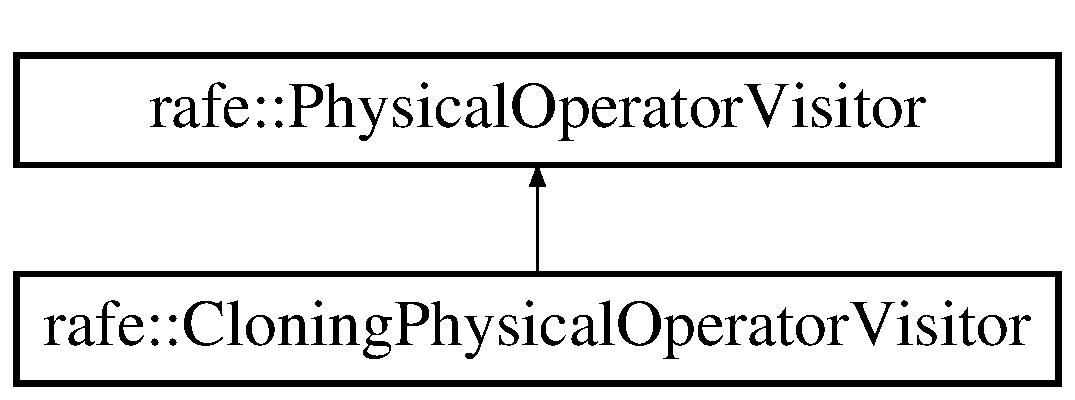
\includegraphics[height=2.000000cm]{classrafe_1_1_cloning_physical_operator_visitor}
\end{center}
\end{figure}
\subsection*{Public Member Functions}
\begin{DoxyCompactItemize}
\item 
void \hyperlink{classrafe_1_1_cloning_physical_operator_visitor_a81fb87714996a1e029da452d2b57796c}{visit\+Filter} (\hyperlink{classrafe_1_1_filter}{Filter} $\ast$node)
\item 
void \hyperlink{classrafe_1_1_cloning_physical_operator_visitor_a885c7ea7353edd39752618c3ae4000ec}{visit\+Filter\+Keeping\+Order} (\hyperlink{classrafe_1_1_filter_keeping_order}{Filter\+Keeping\+Order} $\ast$node)
\item 
void \hyperlink{classrafe_1_1_cloning_physical_operator_visitor_afd4177f24dc58c451d2ca2ce5ed74683}{visit\+Sort\+Operator} (\hyperlink{classrafe_1_1_sort_operator}{Sort\+Operator} $\ast$node)
\item 
void \hyperlink{classrafe_1_1_cloning_physical_operator_visitor_af940eb33c8b37ec531254bbb14d2d2a9}{visit\+Merge\+Equi\+Join} (\hyperlink{classrafe_1_1_merge_equi_join}{Merge\+Equi\+Join} $\ast$node)
\item 
void \hyperlink{classrafe_1_1_cloning_physical_operator_visitor_a9d91a81c0a4e620fb96532388f69bfa1}{visit\+Merge\+Non\+Equi\+Join} (\hyperlink{classrafe_1_1_merge_non_equi_join}{Merge\+Non\+Equi\+Join} $\ast$node)
\item 
void \hyperlink{classrafe_1_1_cloning_physical_operator_visitor_ab0ce6e1f5d26047f898603aeb39278f6}{visit\+Cross\+Join} (\hyperlink{classrafe_1_1_cross_join}{Cross\+Join} $\ast$node)
\item 
void \hyperlink{classrafe_1_1_cloning_physical_operator_visitor_aad57f1f45fa9f3c6633db5421f17774e}{visit\+Hash\+Join} (\hyperlink{classrafe_1_1_hash_join}{Hash\+Join} $\ast$node)
\item 
void \hyperlink{classrafe_1_1_cloning_physical_operator_visitor_a19461012b1f6c83d7b27361b02bf6a7d}{visit\+Hash\+Anti\+Join} (\hyperlink{classrafe_1_1_hash_anti_join}{Hash\+Anti\+Join} $\ast$node)
\item 
void \hyperlink{classrafe_1_1_cloning_physical_operator_visitor_a7e306d085f9a1c0a0cbe7befc79b7e97}{visit\+Merge\+Anti\+Join} (\hyperlink{classrafe_1_1_merge_anti_join}{Merge\+Anti\+Join} $\ast$node)
\item 
void \hyperlink{classrafe_1_1_cloning_physical_operator_visitor_ad8ec858f208334b140f5cb95a01c4063}{visit\+Union\+Operator} (\hyperlink{classrafe_1_1_union_operator}{Union\+Operator} $\ast$node)
\item 
void \hyperlink{classrafe_1_1_cloning_physical_operator_visitor_a489a807271ce26529d48cefea1aa31a2}{visit\+Hash\+Group} (\hyperlink{classrafe_1_1_hash_group}{Hash\+Group} $\ast$node)
\item 
void \hyperlink{classrafe_1_1_cloning_physical_operator_visitor_a5eeb41c81760f9598b11e18ba26949f6}{visit\+Sorted\+Group} (\hyperlink{classrafe_1_1_sorted_group}{Sorted\+Group} $\ast$node)
\item 
void \hyperlink{classrafe_1_1_cloning_physical_operator_visitor_aac8214c9491fac739850b004bad92815}{visit\+Columns\+Operations\+Operator} (\hyperlink{classrafe_1_1_columns_operations_operator}{Columns\+Operations\+Operator} $\ast$node)
\item 
void \hyperlink{classrafe_1_1_cloning_physical_operator_visitor_a61e925129b55230d187280a9a6d76d37}{visit\+Scan\+And\+Sort\+By\+Index} (\hyperlink{classrafe_1_1_scan_and_sort_by_index}{Scan\+And\+Sort\+By\+Index} $\ast$node)
\item 
void \hyperlink{classrafe_1_1_cloning_physical_operator_visitor_a5515f4184243db8a585276d1cb58a8c2}{visit\+Table\+Scan} (\hyperlink{classrafe_1_1_table_scan}{Table\+Scan} $\ast$node)
\item 
void \hyperlink{classrafe_1_1_cloning_physical_operator_visitor_a43fa4aac2e3adfd4b1dc2280a1cfe165}{visit\+Index\+Scan} (\hyperlink{classrafe_1_1_index_scan}{Index\+Scan} $\ast$node)
\end{DoxyCompactItemize}
\subsection*{Public Attributes}
\begin{DoxyCompactItemize}
\item 
std\+::shared\+\_\+ptr$<$ \hyperlink{classrafe_1_1_physical_operator}{Physical\+Operator} $>$ \hyperlink{classrafe_1_1_cloning_physical_operator_visitor_a86bb79f74c796959168c69eeb1d35dea}{result}
\end{DoxyCompactItemize}


\subsection{Detailed Description}
Clones physial operator tree. 

\subsection{Member Function Documentation}
\hypertarget{classrafe_1_1_cloning_physical_operator_visitor_aac8214c9491fac739850b004bad92815}{\index{rafe\+::\+Cloning\+Physical\+Operator\+Visitor@{rafe\+::\+Cloning\+Physical\+Operator\+Visitor}!visit\+Columns\+Operations\+Operator@{visit\+Columns\+Operations\+Operator}}
\index{visit\+Columns\+Operations\+Operator@{visit\+Columns\+Operations\+Operator}!rafe\+::\+Cloning\+Physical\+Operator\+Visitor@{rafe\+::\+Cloning\+Physical\+Operator\+Visitor}}
\subsubsection[{visit\+Columns\+Operations\+Operator}]{\setlength{\rightskip}{0pt plus 5cm}void rafe\+::\+Cloning\+Physical\+Operator\+Visitor\+::visit\+Columns\+Operations\+Operator (
\begin{DoxyParamCaption}
\item[{{\bf Columns\+Operations\+Operator} $\ast$}]{node}
\end{DoxyParamCaption}
)\hspace{0.3cm}{\ttfamily [virtual]}}}\label{classrafe_1_1_cloning_physical_operator_visitor_aac8214c9491fac739850b004bad92815}
Visits physical operator \hyperlink{classrafe_1_1_columns_operations_operator}{Columns\+Operations\+Operator}. 
\begin{DoxyParams}{Parameters}
{\em node} & visited \hyperlink{classrafe_1_1_columns_operations_operator}{Columns\+Operations\+Operator}. \\
\hline
\end{DoxyParams}


Reimplemented from \hyperlink{classrafe_1_1_physical_operator_visitor_ab69b85d7a2c8f89986d84cbcce6f2f89}{rafe\+::\+Physical\+Operator\+Visitor}.

\hypertarget{classrafe_1_1_cloning_physical_operator_visitor_ab0ce6e1f5d26047f898603aeb39278f6}{\index{rafe\+::\+Cloning\+Physical\+Operator\+Visitor@{rafe\+::\+Cloning\+Physical\+Operator\+Visitor}!visit\+Cross\+Join@{visit\+Cross\+Join}}
\index{visit\+Cross\+Join@{visit\+Cross\+Join}!rafe\+::\+Cloning\+Physical\+Operator\+Visitor@{rafe\+::\+Cloning\+Physical\+Operator\+Visitor}}
\subsubsection[{visit\+Cross\+Join}]{\setlength{\rightskip}{0pt plus 5cm}void rafe\+::\+Cloning\+Physical\+Operator\+Visitor\+::visit\+Cross\+Join (
\begin{DoxyParamCaption}
\item[{{\bf Cross\+Join} $\ast$}]{node}
\end{DoxyParamCaption}
)\hspace{0.3cm}{\ttfamily [virtual]}}}\label{classrafe_1_1_cloning_physical_operator_visitor_ab0ce6e1f5d26047f898603aeb39278f6}
Visits physical operator \hyperlink{classrafe_1_1_cross_join}{Cross\+Join}. 
\begin{DoxyParams}{Parameters}
{\em node} & visited \hyperlink{classrafe_1_1_cross_join}{Cross\+Join}. \\
\hline
\end{DoxyParams}


Reimplemented from \hyperlink{classrafe_1_1_physical_operator_visitor_acc39509ae79aa6848ec928cc4f616d61}{rafe\+::\+Physical\+Operator\+Visitor}.

\hypertarget{classrafe_1_1_cloning_physical_operator_visitor_a81fb87714996a1e029da452d2b57796c}{\index{rafe\+::\+Cloning\+Physical\+Operator\+Visitor@{rafe\+::\+Cloning\+Physical\+Operator\+Visitor}!visit\+Filter@{visit\+Filter}}
\index{visit\+Filter@{visit\+Filter}!rafe\+::\+Cloning\+Physical\+Operator\+Visitor@{rafe\+::\+Cloning\+Physical\+Operator\+Visitor}}
\subsubsection[{visit\+Filter}]{\setlength{\rightskip}{0pt plus 5cm}void rafe\+::\+Cloning\+Physical\+Operator\+Visitor\+::visit\+Filter (
\begin{DoxyParamCaption}
\item[{{\bf Filter} $\ast$}]{node}
\end{DoxyParamCaption}
)\hspace{0.3cm}{\ttfamily [virtual]}}}\label{classrafe_1_1_cloning_physical_operator_visitor_a81fb87714996a1e029da452d2b57796c}
Visits physical operator \hyperlink{classrafe_1_1_filter}{Filter}. 
\begin{DoxyParams}{Parameters}
{\em node} & visited \hyperlink{classrafe_1_1_filter}{Filter}. \\
\hline
\end{DoxyParams}


Reimplemented from \hyperlink{classrafe_1_1_physical_operator_visitor_a516a84d305910f3e1b9d1ae2cb184b24}{rafe\+::\+Physical\+Operator\+Visitor}.

\hypertarget{classrafe_1_1_cloning_physical_operator_visitor_a885c7ea7353edd39752618c3ae4000ec}{\index{rafe\+::\+Cloning\+Physical\+Operator\+Visitor@{rafe\+::\+Cloning\+Physical\+Operator\+Visitor}!visit\+Filter\+Keeping\+Order@{visit\+Filter\+Keeping\+Order}}
\index{visit\+Filter\+Keeping\+Order@{visit\+Filter\+Keeping\+Order}!rafe\+::\+Cloning\+Physical\+Operator\+Visitor@{rafe\+::\+Cloning\+Physical\+Operator\+Visitor}}
\subsubsection[{visit\+Filter\+Keeping\+Order}]{\setlength{\rightskip}{0pt plus 5cm}void rafe\+::\+Cloning\+Physical\+Operator\+Visitor\+::visit\+Filter\+Keeping\+Order (
\begin{DoxyParamCaption}
\item[{{\bf Filter\+Keeping\+Order} $\ast$}]{node}
\end{DoxyParamCaption}
)\hspace{0.3cm}{\ttfamily [virtual]}}}\label{classrafe_1_1_cloning_physical_operator_visitor_a885c7ea7353edd39752618c3ae4000ec}
Visits physical operator \hyperlink{classrafe_1_1_filter_keeping_order}{Filter\+Keeping\+Order}. 
\begin{DoxyParams}{Parameters}
{\em node} & visited \hyperlink{classrafe_1_1_filter_keeping_order}{Filter\+Keeping\+Order}. \\
\hline
\end{DoxyParams}


Reimplemented from \hyperlink{classrafe_1_1_physical_operator_visitor_a7b581054d167c71fa5443570a6808740}{rafe\+::\+Physical\+Operator\+Visitor}.

\hypertarget{classrafe_1_1_cloning_physical_operator_visitor_a19461012b1f6c83d7b27361b02bf6a7d}{\index{rafe\+::\+Cloning\+Physical\+Operator\+Visitor@{rafe\+::\+Cloning\+Physical\+Operator\+Visitor}!visit\+Hash\+Anti\+Join@{visit\+Hash\+Anti\+Join}}
\index{visit\+Hash\+Anti\+Join@{visit\+Hash\+Anti\+Join}!rafe\+::\+Cloning\+Physical\+Operator\+Visitor@{rafe\+::\+Cloning\+Physical\+Operator\+Visitor}}
\subsubsection[{visit\+Hash\+Anti\+Join}]{\setlength{\rightskip}{0pt plus 5cm}void rafe\+::\+Cloning\+Physical\+Operator\+Visitor\+::visit\+Hash\+Anti\+Join (
\begin{DoxyParamCaption}
\item[{{\bf Hash\+Anti\+Join} $\ast$}]{node}
\end{DoxyParamCaption}
)\hspace{0.3cm}{\ttfamily [virtual]}}}\label{classrafe_1_1_cloning_physical_operator_visitor_a19461012b1f6c83d7b27361b02bf6a7d}
Visits physical operator \hyperlink{classrafe_1_1_hash_anti_join}{Hash\+Anti\+Join}. 
\begin{DoxyParams}{Parameters}
{\em node} & visited \hyperlink{classrafe_1_1_hash_anti_join}{Hash\+Anti\+Join}. \\
\hline
\end{DoxyParams}


Reimplemented from \hyperlink{classrafe_1_1_physical_operator_visitor_a9415b5939da4948ac922e63fbece1135}{rafe\+::\+Physical\+Operator\+Visitor}.

\hypertarget{classrafe_1_1_cloning_physical_operator_visitor_a489a807271ce26529d48cefea1aa31a2}{\index{rafe\+::\+Cloning\+Physical\+Operator\+Visitor@{rafe\+::\+Cloning\+Physical\+Operator\+Visitor}!visit\+Hash\+Group@{visit\+Hash\+Group}}
\index{visit\+Hash\+Group@{visit\+Hash\+Group}!rafe\+::\+Cloning\+Physical\+Operator\+Visitor@{rafe\+::\+Cloning\+Physical\+Operator\+Visitor}}
\subsubsection[{visit\+Hash\+Group}]{\setlength{\rightskip}{0pt plus 5cm}void rafe\+::\+Cloning\+Physical\+Operator\+Visitor\+::visit\+Hash\+Group (
\begin{DoxyParamCaption}
\item[{{\bf Hash\+Group} $\ast$}]{node}
\end{DoxyParamCaption}
)\hspace{0.3cm}{\ttfamily [virtual]}}}\label{classrafe_1_1_cloning_physical_operator_visitor_a489a807271ce26529d48cefea1aa31a2}
Visits physical operator \hyperlink{classrafe_1_1_hash_group}{Hash\+Group}. 
\begin{DoxyParams}{Parameters}
{\em node} & visited \hyperlink{classrafe_1_1_hash_group}{Hash\+Group}. \\
\hline
\end{DoxyParams}


Reimplemented from \hyperlink{classrafe_1_1_physical_operator_visitor_ab6a2b2b02f2237fd41e6c44f5b2ede9b}{rafe\+::\+Physical\+Operator\+Visitor}.

\hypertarget{classrafe_1_1_cloning_physical_operator_visitor_aad57f1f45fa9f3c6633db5421f17774e}{\index{rafe\+::\+Cloning\+Physical\+Operator\+Visitor@{rafe\+::\+Cloning\+Physical\+Operator\+Visitor}!visit\+Hash\+Join@{visit\+Hash\+Join}}
\index{visit\+Hash\+Join@{visit\+Hash\+Join}!rafe\+::\+Cloning\+Physical\+Operator\+Visitor@{rafe\+::\+Cloning\+Physical\+Operator\+Visitor}}
\subsubsection[{visit\+Hash\+Join}]{\setlength{\rightskip}{0pt plus 5cm}void rafe\+::\+Cloning\+Physical\+Operator\+Visitor\+::visit\+Hash\+Join (
\begin{DoxyParamCaption}
\item[{{\bf Hash\+Join} $\ast$}]{node}
\end{DoxyParamCaption}
)\hspace{0.3cm}{\ttfamily [virtual]}}}\label{classrafe_1_1_cloning_physical_operator_visitor_aad57f1f45fa9f3c6633db5421f17774e}
Visits physical operator \hyperlink{classrafe_1_1_hash_join}{Hash\+Join}. 
\begin{DoxyParams}{Parameters}
{\em node} & visited \hyperlink{classrafe_1_1_hash_join}{Hash\+Join}. \\
\hline
\end{DoxyParams}


Reimplemented from \hyperlink{classrafe_1_1_physical_operator_visitor_ae36c9ef817768f134d35fe5b3834855c}{rafe\+::\+Physical\+Operator\+Visitor}.

\hypertarget{classrafe_1_1_cloning_physical_operator_visitor_a43fa4aac2e3adfd4b1dc2280a1cfe165}{\index{rafe\+::\+Cloning\+Physical\+Operator\+Visitor@{rafe\+::\+Cloning\+Physical\+Operator\+Visitor}!visit\+Index\+Scan@{visit\+Index\+Scan}}
\index{visit\+Index\+Scan@{visit\+Index\+Scan}!rafe\+::\+Cloning\+Physical\+Operator\+Visitor@{rafe\+::\+Cloning\+Physical\+Operator\+Visitor}}
\subsubsection[{visit\+Index\+Scan}]{\setlength{\rightskip}{0pt plus 5cm}void rafe\+::\+Cloning\+Physical\+Operator\+Visitor\+::visit\+Index\+Scan (
\begin{DoxyParamCaption}
\item[{{\bf Index\+Scan} $\ast$}]{node}
\end{DoxyParamCaption}
)\hspace{0.3cm}{\ttfamily [virtual]}}}\label{classrafe_1_1_cloning_physical_operator_visitor_a43fa4aac2e3adfd4b1dc2280a1cfe165}
Visits physical operator \hyperlink{classrafe_1_1_index_scan}{Index\+Scan}. 
\begin{DoxyParams}{Parameters}
{\em node} & visited \hyperlink{classrafe_1_1_index_scan}{Index\+Scan}. \\
\hline
\end{DoxyParams}


Reimplemented from \hyperlink{classrafe_1_1_physical_operator_visitor_ac33ea100cdb3e642a58a82c4367de3fd}{rafe\+::\+Physical\+Operator\+Visitor}.

\hypertarget{classrafe_1_1_cloning_physical_operator_visitor_a7e306d085f9a1c0a0cbe7befc79b7e97}{\index{rafe\+::\+Cloning\+Physical\+Operator\+Visitor@{rafe\+::\+Cloning\+Physical\+Operator\+Visitor}!visit\+Merge\+Anti\+Join@{visit\+Merge\+Anti\+Join}}
\index{visit\+Merge\+Anti\+Join@{visit\+Merge\+Anti\+Join}!rafe\+::\+Cloning\+Physical\+Operator\+Visitor@{rafe\+::\+Cloning\+Physical\+Operator\+Visitor}}
\subsubsection[{visit\+Merge\+Anti\+Join}]{\setlength{\rightskip}{0pt plus 5cm}void rafe\+::\+Cloning\+Physical\+Operator\+Visitor\+::visit\+Merge\+Anti\+Join (
\begin{DoxyParamCaption}
\item[{{\bf Merge\+Anti\+Join} $\ast$}]{node}
\end{DoxyParamCaption}
)\hspace{0.3cm}{\ttfamily [virtual]}}}\label{classrafe_1_1_cloning_physical_operator_visitor_a7e306d085f9a1c0a0cbe7befc79b7e97}
Visits physical operator \hyperlink{classrafe_1_1_merge_anti_join}{Merge\+Anti\+Join}. 
\begin{DoxyParams}{Parameters}
{\em node} & visited \hyperlink{classrafe_1_1_merge_anti_join}{Merge\+Anti\+Join}. \\
\hline
\end{DoxyParams}


Reimplemented from \hyperlink{classrafe_1_1_physical_operator_visitor_a0f3496aaac992756bbb8f18c1000ed75}{rafe\+::\+Physical\+Operator\+Visitor}.

\hypertarget{classrafe_1_1_cloning_physical_operator_visitor_af940eb33c8b37ec531254bbb14d2d2a9}{\index{rafe\+::\+Cloning\+Physical\+Operator\+Visitor@{rafe\+::\+Cloning\+Physical\+Operator\+Visitor}!visit\+Merge\+Equi\+Join@{visit\+Merge\+Equi\+Join}}
\index{visit\+Merge\+Equi\+Join@{visit\+Merge\+Equi\+Join}!rafe\+::\+Cloning\+Physical\+Operator\+Visitor@{rafe\+::\+Cloning\+Physical\+Operator\+Visitor}}
\subsubsection[{visit\+Merge\+Equi\+Join}]{\setlength{\rightskip}{0pt plus 5cm}void rafe\+::\+Cloning\+Physical\+Operator\+Visitor\+::visit\+Merge\+Equi\+Join (
\begin{DoxyParamCaption}
\item[{{\bf Merge\+Equi\+Join} $\ast$}]{node}
\end{DoxyParamCaption}
)\hspace{0.3cm}{\ttfamily [virtual]}}}\label{classrafe_1_1_cloning_physical_operator_visitor_af940eb33c8b37ec531254bbb14d2d2a9}
Visits physical operator \hyperlink{classrafe_1_1_merge_equi_join}{Merge\+Equi\+Join}. 
\begin{DoxyParams}{Parameters}
{\em node} & visited \hyperlink{classrafe_1_1_merge_equi_join}{Merge\+Equi\+Join}. \\
\hline
\end{DoxyParams}


Reimplemented from \hyperlink{classrafe_1_1_physical_operator_visitor_a9fd16981e6fbb9b545b7edeaabcf97bf}{rafe\+::\+Physical\+Operator\+Visitor}.

\hypertarget{classrafe_1_1_cloning_physical_operator_visitor_a9d91a81c0a4e620fb96532388f69bfa1}{\index{rafe\+::\+Cloning\+Physical\+Operator\+Visitor@{rafe\+::\+Cloning\+Physical\+Operator\+Visitor}!visit\+Merge\+Non\+Equi\+Join@{visit\+Merge\+Non\+Equi\+Join}}
\index{visit\+Merge\+Non\+Equi\+Join@{visit\+Merge\+Non\+Equi\+Join}!rafe\+::\+Cloning\+Physical\+Operator\+Visitor@{rafe\+::\+Cloning\+Physical\+Operator\+Visitor}}
\subsubsection[{visit\+Merge\+Non\+Equi\+Join}]{\setlength{\rightskip}{0pt plus 5cm}void rafe\+::\+Cloning\+Physical\+Operator\+Visitor\+::visit\+Merge\+Non\+Equi\+Join (
\begin{DoxyParamCaption}
\item[{{\bf Merge\+Non\+Equi\+Join} $\ast$}]{node}
\end{DoxyParamCaption}
)\hspace{0.3cm}{\ttfamily [virtual]}}}\label{classrafe_1_1_cloning_physical_operator_visitor_a9d91a81c0a4e620fb96532388f69bfa1}
Visits physical operator \hyperlink{classrafe_1_1_merge_non_equi_join}{Merge\+Non\+Equi\+Join}. 
\begin{DoxyParams}{Parameters}
{\em node} & visited \hyperlink{classrafe_1_1_merge_non_equi_join}{Merge\+Non\+Equi\+Join}. \\
\hline
\end{DoxyParams}


Reimplemented from \hyperlink{classrafe_1_1_physical_operator_visitor_a1d4af9c73ece300d7a90c65481cd8e06}{rafe\+::\+Physical\+Operator\+Visitor}.

\hypertarget{classrafe_1_1_cloning_physical_operator_visitor_a61e925129b55230d187280a9a6d76d37}{\index{rafe\+::\+Cloning\+Physical\+Operator\+Visitor@{rafe\+::\+Cloning\+Physical\+Operator\+Visitor}!visit\+Scan\+And\+Sort\+By\+Index@{visit\+Scan\+And\+Sort\+By\+Index}}
\index{visit\+Scan\+And\+Sort\+By\+Index@{visit\+Scan\+And\+Sort\+By\+Index}!rafe\+::\+Cloning\+Physical\+Operator\+Visitor@{rafe\+::\+Cloning\+Physical\+Operator\+Visitor}}
\subsubsection[{visit\+Scan\+And\+Sort\+By\+Index}]{\setlength{\rightskip}{0pt plus 5cm}void rafe\+::\+Cloning\+Physical\+Operator\+Visitor\+::visit\+Scan\+And\+Sort\+By\+Index (
\begin{DoxyParamCaption}
\item[{{\bf Scan\+And\+Sort\+By\+Index} $\ast$}]{node}
\end{DoxyParamCaption}
)\hspace{0.3cm}{\ttfamily [virtual]}}}\label{classrafe_1_1_cloning_physical_operator_visitor_a61e925129b55230d187280a9a6d76d37}
Visits physical operator \hyperlink{classrafe_1_1_scan_and_sort_by_index}{Scan\+And\+Sort\+By\+Index}. 
\begin{DoxyParams}{Parameters}
{\em node} & visited \hyperlink{classrafe_1_1_scan_and_sort_by_index}{Scan\+And\+Sort\+By\+Index}. \\
\hline
\end{DoxyParams}


Reimplemented from \hyperlink{classrafe_1_1_physical_operator_visitor_a4f8cbef9d1c5a58fceb44deb4a7d998c}{rafe\+::\+Physical\+Operator\+Visitor}.

\hypertarget{classrafe_1_1_cloning_physical_operator_visitor_a5eeb41c81760f9598b11e18ba26949f6}{\index{rafe\+::\+Cloning\+Physical\+Operator\+Visitor@{rafe\+::\+Cloning\+Physical\+Operator\+Visitor}!visit\+Sorted\+Group@{visit\+Sorted\+Group}}
\index{visit\+Sorted\+Group@{visit\+Sorted\+Group}!rafe\+::\+Cloning\+Physical\+Operator\+Visitor@{rafe\+::\+Cloning\+Physical\+Operator\+Visitor}}
\subsubsection[{visit\+Sorted\+Group}]{\setlength{\rightskip}{0pt plus 5cm}void rafe\+::\+Cloning\+Physical\+Operator\+Visitor\+::visit\+Sorted\+Group (
\begin{DoxyParamCaption}
\item[{{\bf Sorted\+Group} $\ast$}]{node}
\end{DoxyParamCaption}
)\hspace{0.3cm}{\ttfamily [virtual]}}}\label{classrafe_1_1_cloning_physical_operator_visitor_a5eeb41c81760f9598b11e18ba26949f6}
Visits physical operator \hyperlink{classrafe_1_1_sorted_group}{Sorted\+Group}. 
\begin{DoxyParams}{Parameters}
{\em node} & visited \hyperlink{classrafe_1_1_sorted_group}{Sorted\+Group}. \\
\hline
\end{DoxyParams}


Reimplemented from \hyperlink{classrafe_1_1_physical_operator_visitor_afb1b6786bf12f12e3b1c2895bf77e874}{rafe\+::\+Physical\+Operator\+Visitor}.

\hypertarget{classrafe_1_1_cloning_physical_operator_visitor_afd4177f24dc58c451d2ca2ce5ed74683}{\index{rafe\+::\+Cloning\+Physical\+Operator\+Visitor@{rafe\+::\+Cloning\+Physical\+Operator\+Visitor}!visit\+Sort\+Operator@{visit\+Sort\+Operator}}
\index{visit\+Sort\+Operator@{visit\+Sort\+Operator}!rafe\+::\+Cloning\+Physical\+Operator\+Visitor@{rafe\+::\+Cloning\+Physical\+Operator\+Visitor}}
\subsubsection[{visit\+Sort\+Operator}]{\setlength{\rightskip}{0pt plus 5cm}void rafe\+::\+Cloning\+Physical\+Operator\+Visitor\+::visit\+Sort\+Operator (
\begin{DoxyParamCaption}
\item[{{\bf Sort\+Operator} $\ast$}]{node}
\end{DoxyParamCaption}
)\hspace{0.3cm}{\ttfamily [virtual]}}}\label{classrafe_1_1_cloning_physical_operator_visitor_afd4177f24dc58c451d2ca2ce5ed74683}
Visits physical operator \hyperlink{classrafe_1_1_sort_operator}{Sort\+Operator}. 
\begin{DoxyParams}{Parameters}
{\em node} & visited \hyperlink{classrafe_1_1_sort_operator}{Sort\+Operator}. \\
\hline
\end{DoxyParams}


Reimplemented from \hyperlink{classrafe_1_1_physical_operator_visitor_adaee48b1ef175226c860c7b2d70ba15d}{rafe\+::\+Physical\+Operator\+Visitor}.

\hypertarget{classrafe_1_1_cloning_physical_operator_visitor_a5515f4184243db8a585276d1cb58a8c2}{\index{rafe\+::\+Cloning\+Physical\+Operator\+Visitor@{rafe\+::\+Cloning\+Physical\+Operator\+Visitor}!visit\+Table\+Scan@{visit\+Table\+Scan}}
\index{visit\+Table\+Scan@{visit\+Table\+Scan}!rafe\+::\+Cloning\+Physical\+Operator\+Visitor@{rafe\+::\+Cloning\+Physical\+Operator\+Visitor}}
\subsubsection[{visit\+Table\+Scan}]{\setlength{\rightskip}{0pt plus 5cm}void rafe\+::\+Cloning\+Physical\+Operator\+Visitor\+::visit\+Table\+Scan (
\begin{DoxyParamCaption}
\item[{{\bf Table\+Scan} $\ast$}]{node}
\end{DoxyParamCaption}
)\hspace{0.3cm}{\ttfamily [virtual]}}}\label{classrafe_1_1_cloning_physical_operator_visitor_a5515f4184243db8a585276d1cb58a8c2}
Visits physical operator \hyperlink{classrafe_1_1_table_scan}{Table\+Scan}. 
\begin{DoxyParams}{Parameters}
{\em node} & visited \hyperlink{classrafe_1_1_table_scan}{Table\+Scan}. \\
\hline
\end{DoxyParams}


Reimplemented from \hyperlink{classrafe_1_1_physical_operator_visitor_ae3d5b2b56e9465713c5ecd4e5fcea9c9}{rafe\+::\+Physical\+Operator\+Visitor}.

\hypertarget{classrafe_1_1_cloning_physical_operator_visitor_ad8ec858f208334b140f5cb95a01c4063}{\index{rafe\+::\+Cloning\+Physical\+Operator\+Visitor@{rafe\+::\+Cloning\+Physical\+Operator\+Visitor}!visit\+Union\+Operator@{visit\+Union\+Operator}}
\index{visit\+Union\+Operator@{visit\+Union\+Operator}!rafe\+::\+Cloning\+Physical\+Operator\+Visitor@{rafe\+::\+Cloning\+Physical\+Operator\+Visitor}}
\subsubsection[{visit\+Union\+Operator}]{\setlength{\rightskip}{0pt plus 5cm}void rafe\+::\+Cloning\+Physical\+Operator\+Visitor\+::visit\+Union\+Operator (
\begin{DoxyParamCaption}
\item[{{\bf Union\+Operator} $\ast$}]{node}
\end{DoxyParamCaption}
)\hspace{0.3cm}{\ttfamily [virtual]}}}\label{classrafe_1_1_cloning_physical_operator_visitor_ad8ec858f208334b140f5cb95a01c4063}
Visits physical operator \hyperlink{classrafe_1_1_union_operator}{Union\+Operator}. 
\begin{DoxyParams}{Parameters}
{\em node} & visited \hyperlink{classrafe_1_1_union_operator}{Union\+Operator}. \\
\hline
\end{DoxyParams}


Reimplemented from \hyperlink{classrafe_1_1_physical_operator_visitor_a01eb10e07cc1fbe7622bc1eb01fa3b79}{rafe\+::\+Physical\+Operator\+Visitor}.



\subsection{Member Data Documentation}
\hypertarget{classrafe_1_1_cloning_physical_operator_visitor_a86bb79f74c796959168c69eeb1d35dea}{\index{rafe\+::\+Cloning\+Physical\+Operator\+Visitor@{rafe\+::\+Cloning\+Physical\+Operator\+Visitor}!result@{result}}
\index{result@{result}!rafe\+::\+Cloning\+Physical\+Operator\+Visitor@{rafe\+::\+Cloning\+Physical\+Operator\+Visitor}}
\subsubsection[{result}]{\setlength{\rightskip}{0pt plus 5cm}std\+::shared\+\_\+ptr$<${\bf Physical\+Operator}$>$ rafe\+::\+Cloning\+Physical\+Operator\+Visitor\+::result}}\label{classrafe_1_1_cloning_physical_operator_visitor_a86bb79f74c796959168c69eeb1d35dea}
Cloned result. 

The documentation for this class was generated from the following files\+:\begin{DoxyCompactItemize}
\item 
C\+:/\+Users/\+Marcel/\+Documents/\+Visual Studio 2012/\+Projects/\+Relational\+Query\+Evaluator/\+Relational\+Query\+Evaluator/Physical\+Operator\+Visitor.\+h\item 
C\+:/\+Users/\+Marcel/\+Documents/\+Visual Studio 2012/\+Projects/\+Relational\+Query\+Evaluator/\+Relational\+Query\+Evaluator/Physical\+Operator\+Visitor.\+cpp\end{DoxyCompactItemize}

\hypertarget{classrafe_1_1_column}{\section{rafe\+:\+:Column Class Reference}
\label{classrafe_1_1_column}\index{rafe\+::\+Column@{rafe\+::\+Column}}
}


{\ttfamily \#include $<$Expressions.\+h$>$}

Inheritance diagram for rafe\+:\+:Column\+:\begin{figure}[H]
\begin{center}
\leavevmode
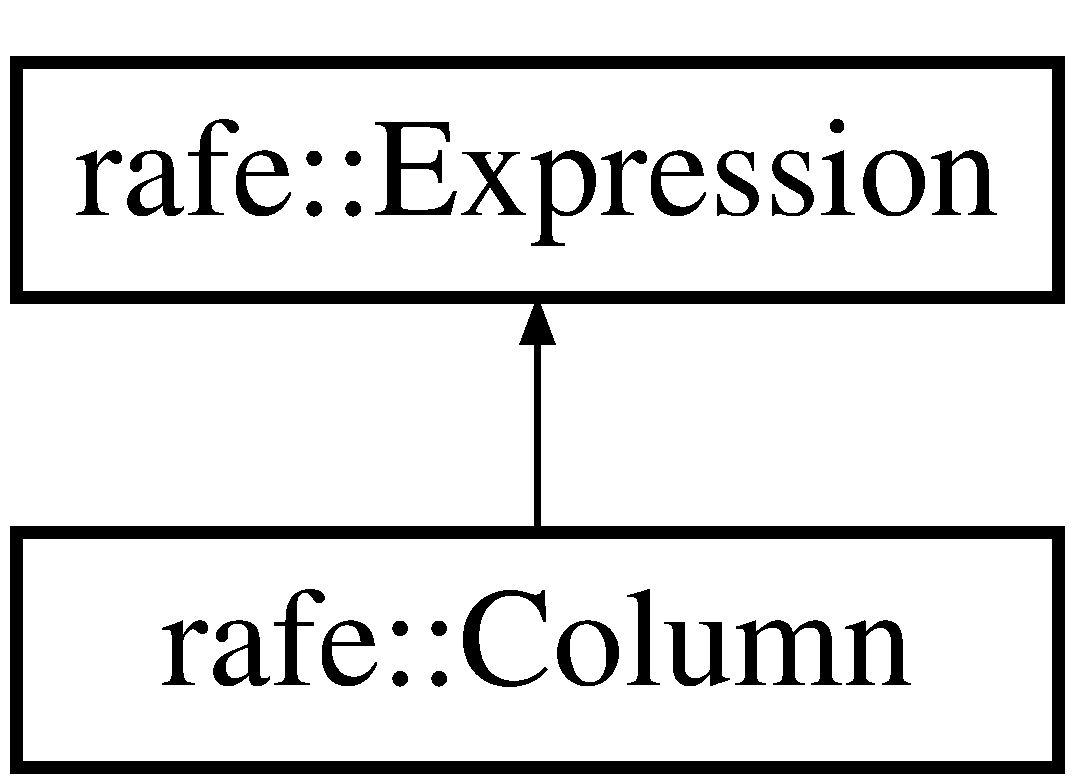
\includegraphics[height=2.000000cm]{classrafe_1_1_column}
\end{center}
\end{figure}
\subsection*{Public Member Functions}
\begin{DoxyCompactItemize}
\item 
\hyperlink{classrafe_1_1_column_a040c4db6ffc5c18a2df387beacdcddc8}{Column} (D\+O\+M\+Element $\ast$node)
\item 
void \hyperlink{classrafe_1_1_column_addd58ca5abdbba013b744ee6a96de75d}{accept} (\hyperlink{classrafe_1_1_expression_visitor_base}{Expression\+Visitor\+Base} \&v)
\item 
void \hyperlink{classrafe_1_1_column_a420f51cd25221b94cbc0dcb7391ee950}{replace\+Child} (\hyperlink{classrafe_1_1_expression}{Expression} $\ast$old\+Child, std\+::shared\+\_\+ptr$<$ \hyperlink{classrafe_1_1_expression}{Expression} $>$ new\+Child)
\end{DoxyCompactItemize}
\subsection*{Public Attributes}
\begin{DoxyCompactItemize}
\item 
\hyperlink{classrafe_1_1_column_identifier}{Column\+Identifier} \hyperlink{classrafe_1_1_column_a7d991e6ad44729235c31910dcc885c5d}{column}
\item 
std\+::string \hyperlink{classrafe_1_1_column_a3e812878630c51153a69f372b1472ce6}{type}
\item 
ulong \hyperlink{classrafe_1_1_column_a1d4d38a6c74a83602c193c5a51f20780}{input}
\end{DoxyCompactItemize}
\subsection*{Additional Inherited Members}


\subsection{Detailed Description}
Represents table column in expression tree. 

\subsection{Constructor \& Destructor Documentation}
\hypertarget{classrafe_1_1_column_a040c4db6ffc5c18a2df387beacdcddc8}{\index{rafe\+::\+Column@{rafe\+::\+Column}!Column@{Column}}
\index{Column@{Column}!rafe\+::\+Column@{rafe\+::\+Column}}
\subsubsection[{Column}]{\setlength{\rightskip}{0pt plus 5cm}rafe\+::\+Column\+::\+Column (
\begin{DoxyParamCaption}
\item[{D\+O\+M\+Element $\ast$}]{node}
\end{DoxyParamCaption}
)}}\label{classrafe_1_1_column_a040c4db6ffc5c18a2df387beacdcddc8}
Creates new instance of \hyperlink{classrafe_1_1_column}{Column}. 
\begin{DoxyParams}{Parameters}
{\em node} & -\/ element storing information about column. \\
\hline
\end{DoxyParams}


\subsection{Member Function Documentation}
\hypertarget{classrafe_1_1_column_addd58ca5abdbba013b744ee6a96de75d}{\index{rafe\+::\+Column@{rafe\+::\+Column}!accept@{accept}}
\index{accept@{accept}!rafe\+::\+Column@{rafe\+::\+Column}}
\subsubsection[{accept}]{\setlength{\rightskip}{0pt plus 5cm}void rafe\+::\+Column\+::accept (
\begin{DoxyParamCaption}
\item[{{\bf Expression\+Visitor\+Base} \&}]{v}
\end{DoxyParamCaption}
)\hspace{0.3cm}{\ttfamily [virtual]}}}\label{classrafe_1_1_column_addd58ca5abdbba013b744ee6a96de75d}
Method for calling visit\mbox{[}node\mbox{]} on given Expression\+Visitor. 
\begin{DoxyParams}{Parameters}
{\em v} & Expression\+Visitor, on which to call visit function. \\
\hline
\end{DoxyParams}


Implements \hyperlink{classrafe_1_1_expression_a3b2e5bae8b99ea6c9a3c92a9b949b3cd}{rafe\+::\+Expression}.

\hypertarget{classrafe_1_1_column_a420f51cd25221b94cbc0dcb7391ee950}{\index{rafe\+::\+Column@{rafe\+::\+Column}!replace\+Child@{replace\+Child}}
\index{replace\+Child@{replace\+Child}!rafe\+::\+Column@{rafe\+::\+Column}}
\subsubsection[{replace\+Child}]{\setlength{\rightskip}{0pt plus 5cm}void rafe\+::\+Column\+::replace\+Child (
\begin{DoxyParamCaption}
\item[{{\bf Expression} $\ast$}]{old\+Child, }
\item[{std\+::shared\+\_\+ptr$<$ {\bf Expression} $>$}]{new\+Child}
\end{DoxyParamCaption}
)\hspace{0.3cm}{\ttfamily [virtual]}}}\label{classrafe_1_1_column_a420f51cd25221b94cbc0dcb7391ee950}
Replaces child from this class with new expression tree. 
\begin{DoxyParams}{Parameters}
{\em old\+Child} & -\/ child to replace. \\
\hline
{\em new\+Child} & -\/ child to be replaced. \\
\hline
\end{DoxyParams}


Implements \hyperlink{classrafe_1_1_expression_a841879e8eb85f4bb68cfeec24231a701}{rafe\+::\+Expression}.



\subsection{Member Data Documentation}
\hypertarget{classrafe_1_1_column_a7d991e6ad44729235c31910dcc885c5d}{\index{rafe\+::\+Column@{rafe\+::\+Column}!column@{column}}
\index{column@{column}!rafe\+::\+Column@{rafe\+::\+Column}}
\subsubsection[{column}]{\setlength{\rightskip}{0pt plus 5cm}{\bf Column\+Identifier} rafe\+::\+Column\+::column}}\label{classrafe_1_1_column_a7d991e6ad44729235c31910dcc885c5d}
Identifies column with name and unique id. \hypertarget{classrafe_1_1_column_a1d4d38a6c74a83602c193c5a51f20780}{\index{rafe\+::\+Column@{rafe\+::\+Column}!input@{input}}
\index{input@{input}!rafe\+::\+Column@{rafe\+::\+Column}}
\subsubsection[{input}]{\setlength{\rightskip}{0pt plus 5cm}ulong rafe\+::\+Column\+::input}}\label{classrafe_1_1_column_a1d4d38a6c74a83602c193c5a51f20780}
This field is used for identifing relation of the column. \hypertarget{classrafe_1_1_column_a3e812878630c51153a69f372b1472ce6}{\index{rafe\+::\+Column@{rafe\+::\+Column}!type@{type}}
\index{type@{type}!rafe\+::\+Column@{rafe\+::\+Column}}
\subsubsection[{type}]{\setlength{\rightskip}{0pt plus 5cm}std\+::string rafe\+::\+Column\+::type}}\label{classrafe_1_1_column_a3e812878630c51153a69f372b1472ce6}
Type of the values stored in the column. 

The documentation for this class was generated from the following files\+:\begin{DoxyCompactItemize}
\item 
C\+:/\+Users/\+Marcel/\+Documents/\+Visual Studio 2012/\+Projects/\+Relational\+Query\+Evaluator/\+Relational\+Query\+Evaluator/Expressions.\+h\item 
C\+:/\+Users/\+Marcel/\+Documents/\+Visual Studio 2012/\+Projects/\+Relational\+Query\+Evaluator/\+Relational\+Query\+Evaluator/Expressions.\+cpp\end{DoxyCompactItemize}

\hypertarget{classrafe_1_1_column_identifier}{\section{rafe\+:\+:Column\+Identifier Class Reference}
\label{classrafe_1_1_column_identifier}\index{rafe\+::\+Column\+Identifier@{rafe\+::\+Column\+Identifier}}
}


{\ttfamily \#include $<$Algebra\+Structures.\+h$>$}

\subsection*{Public Member Functions}
\begin{DoxyCompactItemize}
\item 
\hyperlink{classrafe_1_1_column_identifier_a9893d91ff339d89a2d032adfb63aa11d}{Column\+Identifier} (std\+::string \hyperlink{classrafe_1_1_column_identifier_a65aaf13619c20f17be5f8bdda2c6d28f}{name}, int \hyperlink{classrafe_1_1_column_identifier_afa735a6e57d40b1d7e25c6cc781d3a4d}{id})
\item 
\hyperlink{classrafe_1_1_column_identifier_ab1421d1d15f6d4bb548b7c6727121773}{Column\+Identifier} (std\+::string \hyperlink{classrafe_1_1_column_identifier_a65aaf13619c20f17be5f8bdda2c6d28f}{name})
\item 
\hyperlink{classrafe_1_1_column_identifier_a48f0facd564ddc904cc43c56bfff249f}{Column\+Identifier} ()
\item 
std\+::string \hyperlink{classrafe_1_1_column_identifier_a60033c2c50b301dd5582957978bba2e5}{to\+String} () const 
\item 
bool \hyperlink{classrafe_1_1_column_identifier_a2bfacd7aa1922c35ea93127e3f4b290f}{operator$<$} (const \hyperlink{classrafe_1_1_column_identifier}{Column\+Identifier} \&other) const 
\item 
bool \hyperlink{classrafe_1_1_column_identifier_aa0d0f99b98e2d48b9dacfc3a430a9e52}{operator==} (const \hyperlink{classrafe_1_1_column_identifier}{Column\+Identifier} \&other) const 
\end{DoxyCompactItemize}
\subsection*{Public Attributes}
\begin{DoxyCompactItemize}
\item 
std\+::string \hyperlink{classrafe_1_1_column_identifier_a65aaf13619c20f17be5f8bdda2c6d28f}{name}
\item 
int \hyperlink{classrafe_1_1_column_identifier_afa735a6e57d40b1d7e25c6cc781d3a4d}{id}
\end{DoxyCompactItemize}


\subsection{Detailed Description}
Stres unique indetification of a column. 

\subsection{Constructor \& Destructor Documentation}
\hypertarget{classrafe_1_1_column_identifier_a9893d91ff339d89a2d032adfb63aa11d}{\index{rafe\+::\+Column\+Identifier@{rafe\+::\+Column\+Identifier}!Column\+Identifier@{Column\+Identifier}}
\index{Column\+Identifier@{Column\+Identifier}!rafe\+::\+Column\+Identifier@{rafe\+::\+Column\+Identifier}}
\subsubsection[{Column\+Identifier}]{\setlength{\rightskip}{0pt plus 5cm}rafe\+::\+Column\+Identifier\+::\+Column\+Identifier (
\begin{DoxyParamCaption}
\item[{std\+::string}]{name, }
\item[{int}]{id}
\end{DoxyParamCaption}
)}}\label{classrafe_1_1_column_identifier_a9893d91ff339d89a2d032adfb63aa11d}
Create the instance of \hyperlink{classrafe_1_1_column_identifier}{Column\+Identifier}. 
\begin{DoxyParams}{Parameters}
{\em name} & -\/ column name. \\
\hline
{\em id} & -\/ column unique identifier. \\
\hline
\end{DoxyParams}
\hypertarget{classrafe_1_1_column_identifier_ab1421d1d15f6d4bb548b7c6727121773}{\index{rafe\+::\+Column\+Identifier@{rafe\+::\+Column\+Identifier}!Column\+Identifier@{Column\+Identifier}}
\index{Column\+Identifier@{Column\+Identifier}!rafe\+::\+Column\+Identifier@{rafe\+::\+Column\+Identifier}}
\subsubsection[{Column\+Identifier}]{\setlength{\rightskip}{0pt plus 5cm}rafe\+::\+Column\+Identifier\+::\+Column\+Identifier (
\begin{DoxyParamCaption}
\item[{std\+::string}]{name}
\end{DoxyParamCaption}
)}}\label{classrafe_1_1_column_identifier_ab1421d1d15f6d4bb548b7c6727121773}
Create the instance of \hyperlink{classrafe_1_1_column_identifier}{Column\+Identifier}. 
\begin{DoxyParams}{Parameters}
{\em name} & -\/ column name. \\
\hline
\end{DoxyParams}
\hypertarget{classrafe_1_1_column_identifier_a48f0facd564ddc904cc43c56bfff249f}{\index{rafe\+::\+Column\+Identifier@{rafe\+::\+Column\+Identifier}!Column\+Identifier@{Column\+Identifier}}
\index{Column\+Identifier@{Column\+Identifier}!rafe\+::\+Column\+Identifier@{rafe\+::\+Column\+Identifier}}
\subsubsection[{Column\+Identifier}]{\setlength{\rightskip}{0pt plus 5cm}rafe\+::\+Column\+Identifier\+::\+Column\+Identifier (
\begin{DoxyParamCaption}
{}
\end{DoxyParamCaption}
)}}\label{classrafe_1_1_column_identifier_a48f0facd564ddc904cc43c56bfff249f}
Create the instance of \hyperlink{classrafe_1_1_column_identifier}{Column\+Identifier}. 

\subsection{Member Function Documentation}
\hypertarget{classrafe_1_1_column_identifier_a2bfacd7aa1922c35ea93127e3f4b290f}{\index{rafe\+::\+Column\+Identifier@{rafe\+::\+Column\+Identifier}!operator$<$@{operator$<$}}
\index{operator$<$@{operator$<$}!rafe\+::\+Column\+Identifier@{rafe\+::\+Column\+Identifier}}
\subsubsection[{operator$<$}]{\setlength{\rightskip}{0pt plus 5cm}bool rafe\+::\+Column\+Identifier\+::operator$<$ (
\begin{DoxyParamCaption}
\item[{const {\bf Column\+Identifier} \&}]{other}
\end{DoxyParamCaption}
) const}}\label{classrafe_1_1_column_identifier_a2bfacd7aa1922c35ea93127e3f4b290f}
Compares id of \hyperlink{classrafe_1_1_column_identifier}{Column\+Identifier} so it can be stored in map and set. \hypertarget{classrafe_1_1_column_identifier_aa0d0f99b98e2d48b9dacfc3a430a9e52}{\index{rafe\+::\+Column\+Identifier@{rafe\+::\+Column\+Identifier}!operator==@{operator==}}
\index{operator==@{operator==}!rafe\+::\+Column\+Identifier@{rafe\+::\+Column\+Identifier}}
\subsubsection[{operator==}]{\setlength{\rightskip}{0pt plus 5cm}bool rafe\+::\+Column\+Identifier\+::operator== (
\begin{DoxyParamCaption}
\item[{const {\bf Column\+Identifier} \&}]{other}
\end{DoxyParamCaption}
) const}}\label{classrafe_1_1_column_identifier_aa0d0f99b98e2d48b9dacfc3a430a9e52}
Overload opeartor == and compares only ids. \hypertarget{classrafe_1_1_column_identifier_a60033c2c50b301dd5582957978bba2e5}{\index{rafe\+::\+Column\+Identifier@{rafe\+::\+Column\+Identifier}!to\+String@{to\+String}}
\index{to\+String@{to\+String}!rafe\+::\+Column\+Identifier@{rafe\+::\+Column\+Identifier}}
\subsubsection[{to\+String}]{\setlength{\rightskip}{0pt plus 5cm}string rafe\+::\+Column\+Identifier\+::to\+String (
\begin{DoxyParamCaption}
{}
\end{DoxyParamCaption}
) const}}\label{classrafe_1_1_column_identifier_a60033c2c50b301dd5582957978bba2e5}
\begin{DoxyReturn}{Returns}
String representation of this class. 
\end{DoxyReturn}


\subsection{Member Data Documentation}
\hypertarget{classrafe_1_1_column_identifier_afa735a6e57d40b1d7e25c6cc781d3a4d}{\index{rafe\+::\+Column\+Identifier@{rafe\+::\+Column\+Identifier}!id@{id}}
\index{id@{id}!rafe\+::\+Column\+Identifier@{rafe\+::\+Column\+Identifier}}
\subsubsection[{id}]{\setlength{\rightskip}{0pt plus 5cm}int rafe\+::\+Column\+Identifier\+::id}}\label{classrafe_1_1_column_identifier_afa735a6e57d40b1d7e25c6cc781d3a4d}
Stores unique identifier of a column. \hypertarget{classrafe_1_1_column_identifier_a65aaf13619c20f17be5f8bdda2c6d28f}{\index{rafe\+::\+Column\+Identifier@{rafe\+::\+Column\+Identifier}!name@{name}}
\index{name@{name}!rafe\+::\+Column\+Identifier@{rafe\+::\+Column\+Identifier}}
\subsubsection[{name}]{\setlength{\rightskip}{0pt plus 5cm}std\+::string rafe\+::\+Column\+Identifier\+::name}}\label{classrafe_1_1_column_identifier_a65aaf13619c20f17be5f8bdda2c6d28f}
Stores name of the column. 

The documentation for this class was generated from the following files\+:\begin{DoxyCompactItemize}
\item 
C\+:/\+Users/\+Marcel/\+Documents/\+Visual Studio 2012/\+Projects/\+Relational\+Query\+Evaluator/\+Relational\+Query\+Evaluator/Algebra\+Structures.\+h\item 
C\+:/\+Users/\+Marcel/\+Documents/\+Visual Studio 2012/\+Projects/\+Relational\+Query\+Evaluator/\+Relational\+Query\+Evaluator/Algebra\+Structures.\+cpp\end{DoxyCompactItemize}

\hypertarget{classrafe_1_1_column_info}{\section{rafe\+:\+:Column\+Info Class Reference}
\label{classrafe_1_1_column_info}\index{rafe\+::\+Column\+Info@{rafe\+::\+Column\+Info}}
}


{\ttfamily \#include $<$Algebra\+Structures.\+h$>$}

Inheritance diagram for rafe\+:\+:Column\+Info\+:\begin{figure}[H]
\begin{center}
\leavevmode
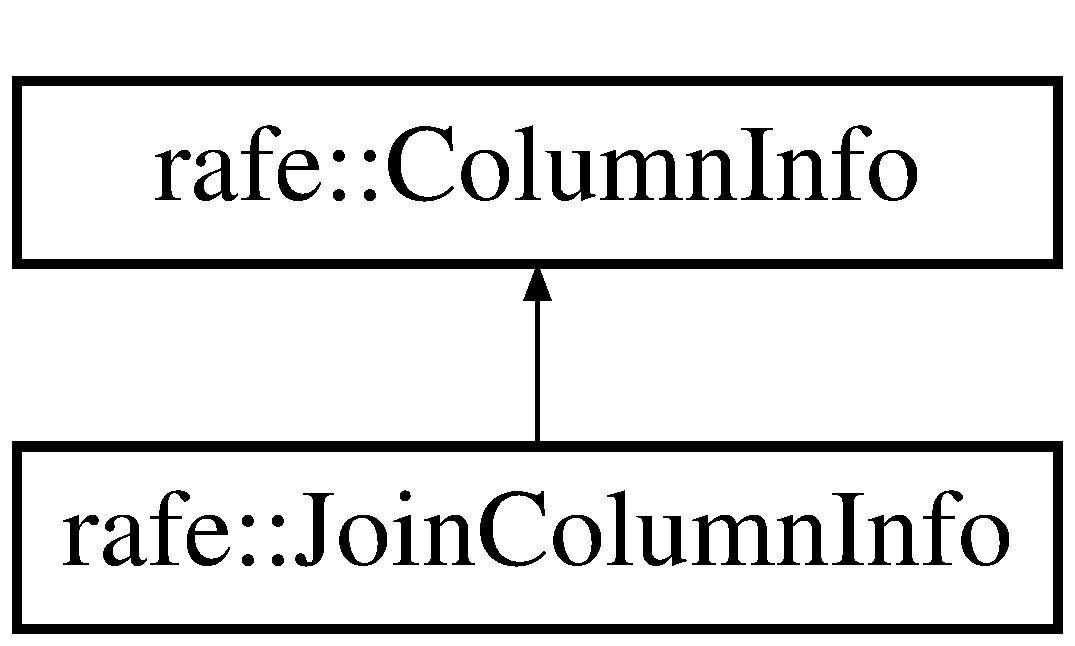
\includegraphics[height=2.000000cm]{classrafe_1_1_column_info}
\end{center}
\end{figure}
\subsection*{Public Member Functions}
\begin{DoxyCompactItemize}
\item 
\hyperlink{classrafe_1_1_column_info_a7b8526771896d312ac4329592fe85f73}{Column\+Info} (std\+::string name, std\+::string \hyperlink{classrafe_1_1_column_info_a22fd355567e1d07f30fd1deae721577f}{type})
\item 
\hyperlink{classrafe_1_1_column_info_a7002d12c04ff1acb398f01b09b3f9297}{Column\+Info} ()
\item 
\hyperlink{classrafe_1_1_column_info_af1b1e671898270d7cd905860297a1707}{Column\+Info} (std\+::string name, double \hyperlink{classrafe_1_1_column_info_a3925986dda2c3385a512d6491e282aae}{number\+Of\+Unique\+Values}, std\+::string \hyperlink{classrafe_1_1_column_info_a22fd355567e1d07f30fd1deae721577f}{type})
\item 
\hyperlink{classrafe_1_1_column_info_a2a9a69f1dfc6a40b2effb352887acba0}{Column\+Info} (const \hyperlink{classrafe_1_1_column_identifier}{Column\+Identifier} \&\hyperlink{classrafe_1_1_column_info_a446710a3a03b249da265a785aff1ee18}{column}, double \hyperlink{classrafe_1_1_column_info_a3925986dda2c3385a512d6491e282aae}{number\+Of\+Unique\+Values}, std\+::string \hyperlink{classrafe_1_1_column_info_a22fd355567e1d07f30fd1deae721577f}{type})
\item 
\hyperlink{classrafe_1_1_column_info_a8e4ca4421d5c611b689421e0feca1114}{Column\+Info} (const \hyperlink{classrafe_1_1_join_column_info}{Join\+Column\+Info} \&info)
\end{DoxyCompactItemize}
\subsection*{Public Attributes}
\begin{DoxyCompactItemize}
\item 
\hyperlink{classrafe_1_1_column_identifier}{Column\+Identifier} \hyperlink{classrafe_1_1_column_info_a446710a3a03b249da265a785aff1ee18}{column}
\item 
std\+::string \hyperlink{classrafe_1_1_column_info_a22fd355567e1d07f30fd1deae721577f}{type}
\item 
double \hyperlink{classrafe_1_1_column_info_a3925986dda2c3385a512d6491e282aae}{number\+Of\+Unique\+Values}
\end{DoxyCompactItemize}


\subsection{Detailed Description}
Stored information about column, like identifier, number of unique values and type. 

\subsection{Constructor \& Destructor Documentation}
\hypertarget{classrafe_1_1_column_info_a7b8526771896d312ac4329592fe85f73}{\index{rafe\+::\+Column\+Info@{rafe\+::\+Column\+Info}!Column\+Info@{Column\+Info}}
\index{Column\+Info@{Column\+Info}!rafe\+::\+Column\+Info@{rafe\+::\+Column\+Info}}
\subsubsection[{Column\+Info}]{\setlength{\rightskip}{0pt plus 5cm}rafe\+::\+Column\+Info\+::\+Column\+Info (
\begin{DoxyParamCaption}
\item[{std\+::string}]{name, }
\item[{std\+::string}]{type}
\end{DoxyParamCaption}
)}}\label{classrafe_1_1_column_info_a7b8526771896d312ac4329592fe85f73}
Create the instance of \hyperlink{classrafe_1_1_column_info}{Column\+Info}. 
\begin{DoxyParams}{Parameters}
{\em name} & -\/ column name \\
\hline
{\em type} & -\/ column type \\
\hline
\end{DoxyParams}
\hypertarget{classrafe_1_1_column_info_a7002d12c04ff1acb398f01b09b3f9297}{\index{rafe\+::\+Column\+Info@{rafe\+::\+Column\+Info}!Column\+Info@{Column\+Info}}
\index{Column\+Info@{Column\+Info}!rafe\+::\+Column\+Info@{rafe\+::\+Column\+Info}}
\subsubsection[{Column\+Info}]{\setlength{\rightskip}{0pt plus 5cm}rafe\+::\+Column\+Info\+::\+Column\+Info (
\begin{DoxyParamCaption}
{}
\end{DoxyParamCaption}
)}}\label{classrafe_1_1_column_info_a7002d12c04ff1acb398f01b09b3f9297}
Create the instance of \hyperlink{classrafe_1_1_column_info}{Column\+Info}. \hypertarget{classrafe_1_1_column_info_af1b1e671898270d7cd905860297a1707}{\index{rafe\+::\+Column\+Info@{rafe\+::\+Column\+Info}!Column\+Info@{Column\+Info}}
\index{Column\+Info@{Column\+Info}!rafe\+::\+Column\+Info@{rafe\+::\+Column\+Info}}
\subsubsection[{Column\+Info}]{\setlength{\rightskip}{0pt plus 5cm}rafe\+::\+Column\+Info\+::\+Column\+Info (
\begin{DoxyParamCaption}
\item[{std\+::string}]{name, }
\item[{double}]{number\+Of\+Unique\+Values, }
\item[{std\+::string}]{type}
\end{DoxyParamCaption}
)}}\label{classrafe_1_1_column_info_af1b1e671898270d7cd905860297a1707}
Create the instance of \hyperlink{classrafe_1_1_column_info}{Column\+Info}. 
\begin{DoxyParams}{Parameters}
{\em name} & -\/ column name \\
\hline
{\em number\+Of\+Unique\+Values} & \\
\hline
{\em type} & -\/ type of column \\
\hline
\end{DoxyParams}
\hypertarget{classrafe_1_1_column_info_a2a9a69f1dfc6a40b2effb352887acba0}{\index{rafe\+::\+Column\+Info@{rafe\+::\+Column\+Info}!Column\+Info@{Column\+Info}}
\index{Column\+Info@{Column\+Info}!rafe\+::\+Column\+Info@{rafe\+::\+Column\+Info}}
\subsubsection[{Column\+Info}]{\setlength{\rightskip}{0pt plus 5cm}rafe\+::\+Column\+Info\+::\+Column\+Info (
\begin{DoxyParamCaption}
\item[{const {\bf Column\+Identifier} \&}]{column, }
\item[{double}]{number\+Of\+Unique\+Values, }
\item[{std\+::string}]{type}
\end{DoxyParamCaption}
)}}\label{classrafe_1_1_column_info_a2a9a69f1dfc6a40b2effb352887acba0}
Create the instance of \hyperlink{classrafe_1_1_column_info}{Column\+Info}. 
\begin{DoxyParams}{Parameters}
{\em column} & -\/ \hyperlink{classrafe_1_1_column_identifier}{Column\+Identifier} of the column \\
\hline
{\em number\+Of\+Unique\+Values} & \\
\hline
{\em type} & -\/ type of column \\
\hline
\end{DoxyParams}
\hypertarget{classrafe_1_1_column_info_a8e4ca4421d5c611b689421e0feca1114}{\index{rafe\+::\+Column\+Info@{rafe\+::\+Column\+Info}!Column\+Info@{Column\+Info}}
\index{Column\+Info@{Column\+Info}!rafe\+::\+Column\+Info@{rafe\+::\+Column\+Info}}
\subsubsection[{Column\+Info}]{\setlength{\rightskip}{0pt plus 5cm}rafe\+::\+Column\+Info\+::\+Column\+Info (
\begin{DoxyParamCaption}
\item[{const {\bf Join\+Column\+Info} \&}]{info}
\end{DoxyParamCaption}
)}}\label{classrafe_1_1_column_info_a8e4ca4421d5c611b689421e0feca1114}
Create the instance of \hyperlink{classrafe_1_1_column_info}{Column\+Info}. 
\begin{DoxyParams}{Parameters}
{\em info} & -\/ \hyperlink{classrafe_1_1_join_column_info}{Join\+Column\+Info} \\
\hline
\end{DoxyParams}


\subsection{Member Data Documentation}
\hypertarget{classrafe_1_1_column_info_a446710a3a03b249da265a785aff1ee18}{\index{rafe\+::\+Column\+Info@{rafe\+::\+Column\+Info}!column@{column}}
\index{column@{column}!rafe\+::\+Column\+Info@{rafe\+::\+Column\+Info}}
\subsubsection[{column}]{\setlength{\rightskip}{0pt plus 5cm}{\bf Column\+Identifier} rafe\+::\+Column\+Info\+::column}}\label{classrafe_1_1_column_info_a446710a3a03b249da265a785aff1ee18}
Columns identifier. \hypertarget{classrafe_1_1_column_info_a3925986dda2c3385a512d6491e282aae}{\index{rafe\+::\+Column\+Info@{rafe\+::\+Column\+Info}!number\+Of\+Unique\+Values@{number\+Of\+Unique\+Values}}
\index{number\+Of\+Unique\+Values@{number\+Of\+Unique\+Values}!rafe\+::\+Column\+Info@{rafe\+::\+Column\+Info}}
\subsubsection[{number\+Of\+Unique\+Values}]{\setlength{\rightskip}{0pt plus 5cm}double rafe\+::\+Column\+Info\+::number\+Of\+Unique\+Values}}\label{classrafe_1_1_column_info_a3925986dda2c3385a512d6491e282aae}
Stores number of unique values for joining purposes. \hypertarget{classrafe_1_1_column_info_a22fd355567e1d07f30fd1deae721577f}{\index{rafe\+::\+Column\+Info@{rafe\+::\+Column\+Info}!type@{type}}
\index{type@{type}!rafe\+::\+Column\+Info@{rafe\+::\+Column\+Info}}
\subsubsection[{type}]{\setlength{\rightskip}{0pt plus 5cm}std\+::string rafe\+::\+Column\+Info\+::type}}\label{classrafe_1_1_column_info_a22fd355567e1d07f30fd1deae721577f}
Type of the column. 

The documentation for this class was generated from the following files\+:\begin{DoxyCompactItemize}
\item 
C\+:/\+Users/\+Marcel/\+Documents/\+Visual Studio 2012/\+Projects/\+Relational\+Query\+Evaluator/\+Relational\+Query\+Evaluator/Algebra\+Structures.\+h\item 
C\+:/\+Users/\+Marcel/\+Documents/\+Visual Studio 2012/\+Projects/\+Relational\+Query\+Evaluator/\+Relational\+Query\+Evaluator/Algebra\+Structures.\+cpp\end{DoxyCompactItemize}

\hypertarget{classrafe_1_1_column_operation}{\section{rafe\+:\+:Column\+Operation Class Reference}
\label{classrafe_1_1_column_operation}\index{rafe\+::\+Column\+Operation@{rafe\+::\+Column\+Operation}}
}


{\ttfamily \#include $<$Algebra\+Structures.\+h$>$}

\subsection*{Public Attributes}
\begin{DoxyCompactItemize}
\item 
\hyperlink{classrafe_1_1_column_identifier}{Column\+Identifier} \hyperlink{classrafe_1_1_column_operation_a728c264bef7363a5bf0578c49654ea3b}{result}
\item 
std\+::shared\+\_\+ptr$<$ \hyperlink{classrafe_1_1_expression}{Expression} $>$ \hyperlink{classrafe_1_1_column_operation_a33bfeb4554709f96d9945cb2148f095b}{expression}
\item 
std\+::string \hyperlink{classrafe_1_1_column_operation_a1c85fd1a1f9465b33553cbdd6e641a51}{type}
\end{DoxyCompactItemize}


\subsection{Detailed Description}
Stores information about operation on columns from extended projection operator. 

\subsection{Member Data Documentation}
\hypertarget{classrafe_1_1_column_operation_a33bfeb4554709f96d9945cb2148f095b}{\index{rafe\+::\+Column\+Operation@{rafe\+::\+Column\+Operation}!expression@{expression}}
\index{expression@{expression}!rafe\+::\+Column\+Operation@{rafe\+::\+Column\+Operation}}
\subsubsection[{expression}]{\setlength{\rightskip}{0pt plus 5cm}std\+::shared\+\_\+ptr$<${\bf Expression}$>$ rafe\+::\+Column\+Operation\+::expression}}\label{classrafe_1_1_column_operation_a33bfeb4554709f96d9945cb2148f095b}
\hyperlink{classrafe_1_1_expression}{Expression} to compute new column. If it is null column is only copied to output. \hypertarget{classrafe_1_1_column_operation_a728c264bef7363a5bf0578c49654ea3b}{\index{rafe\+::\+Column\+Operation@{rafe\+::\+Column\+Operation}!result@{result}}
\index{result@{result}!rafe\+::\+Column\+Operation@{rafe\+::\+Column\+Operation}}
\subsubsection[{result}]{\setlength{\rightskip}{0pt plus 5cm}{\bf Column\+Identifier} rafe\+::\+Column\+Operation\+::result}}\label{classrafe_1_1_column_operation_a728c264bef7363a5bf0578c49654ea3b}
Identifier of output column. \hypertarget{classrafe_1_1_column_operation_a1c85fd1a1f9465b33553cbdd6e641a51}{\index{rafe\+::\+Column\+Operation@{rafe\+::\+Column\+Operation}!type@{type}}
\index{type@{type}!rafe\+::\+Column\+Operation@{rafe\+::\+Column\+Operation}}
\subsubsection[{type}]{\setlength{\rightskip}{0pt plus 5cm}std\+::string rafe\+::\+Column\+Operation\+::type}}\label{classrafe_1_1_column_operation_a1c85fd1a1f9465b33553cbdd6e641a51}
Type of the column. 

The documentation for this class was generated from the following file\+:\begin{DoxyCompactItemize}
\item 
C\+:/\+Users/\+Marcel/\+Documents/\+Visual Studio 2012/\+Projects/\+Relational\+Query\+Evaluator/\+Relational\+Query\+Evaluator/Algebra\+Structures.\+h\end{DoxyCompactItemize}

\hypertarget{classrafe_1_1_column_operations}{\section{rafe\+:\+:Column\+Operations Class Reference}
\label{classrafe_1_1_column_operations}\index{rafe\+::\+Column\+Operations@{rafe\+::\+Column\+Operations}}
}


{\ttfamily \#include $<$Algebra.\+h$>$}

Inheritance diagram for rafe\+:\+:Column\+Operations\+:\begin{figure}[H]
\begin{center}
\leavevmode
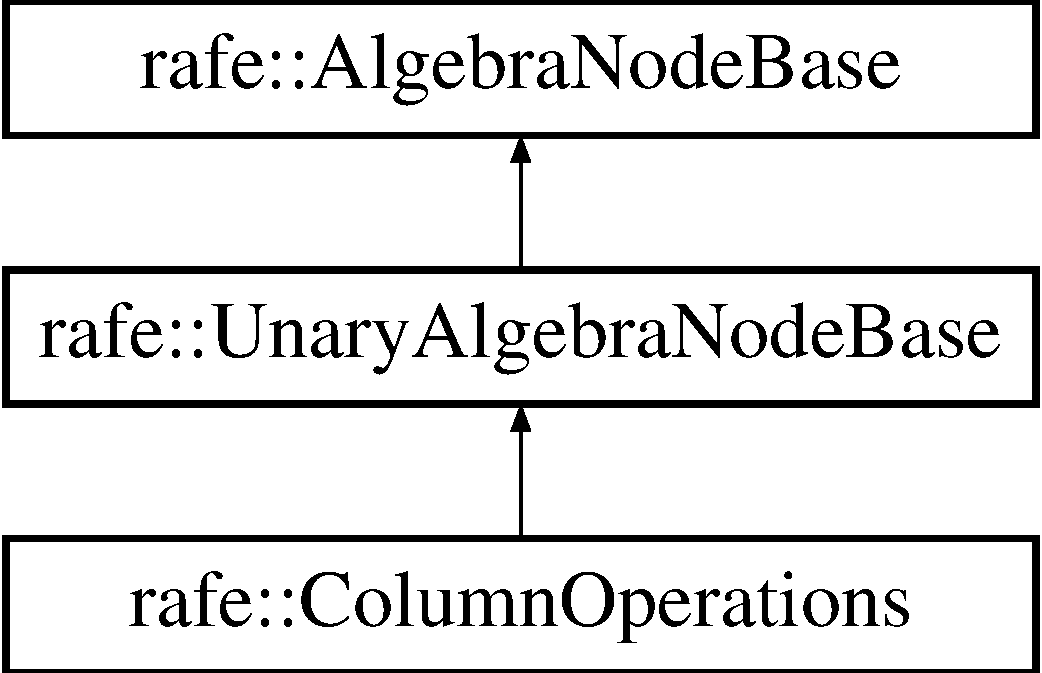
\includegraphics[height=3.000000cm]{classrafe_1_1_column_operations}
\end{center}
\end{figure}
\subsection*{Public Member Functions}
\begin{DoxyCompactItemize}
\item 
\hyperlink{classrafe_1_1_column_operations_a7032e4e6127e60bf523f5a5980459dab}{Column\+Operations} (D\+O\+M\+Element $\ast$element)
\item 
void \hyperlink{classrafe_1_1_column_operations_a3418a59f4befbb949bf14e08d9c7d895}{accept} (\hyperlink{classrafe_1_1_algebra_visitor}{Algebra\+Visitor} \&v)
\end{DoxyCompactItemize}
\subsection*{Public Attributes}
\begin{DoxyCompactItemize}
\item 
std\+::vector$<$ \hyperlink{classrafe_1_1_column_operation}{Column\+Operation} $>$ \hyperlink{classrafe_1_1_column_operations_adb374c76426222828c5b1a6b0f225246}{operations}
\end{DoxyCompactItemize}


\subsection{Detailed Description}
Represents the extended projection. It eliminates some columns and computes new ones using simple operation like +,-\/,$\ast$,/ or other functions. 

\subsection{Constructor \& Destructor Documentation}
\hypertarget{classrafe_1_1_column_operations_a7032e4e6127e60bf523f5a5980459dab}{\index{rafe\+::\+Column\+Operations@{rafe\+::\+Column\+Operations}!Column\+Operations@{Column\+Operations}}
\index{Column\+Operations@{Column\+Operations}!rafe\+::\+Column\+Operations@{rafe\+::\+Column\+Operations}}
\subsubsection[{Column\+Operations}]{\setlength{\rightskip}{0pt plus 5cm}rafe\+::\+Column\+Operations\+::\+Column\+Operations (
\begin{DoxyParamCaption}
\item[{D\+O\+M\+Element $\ast$}]{element}
\end{DoxyParamCaption}
)}}\label{classrafe_1_1_column_operations_a7032e4e6127e60bf523f5a5980459dab}
Creates the instance of \hyperlink{classrafe_1_1_column_operations}{Column\+Operations}. 
\begin{DoxyParams}{Parameters}
{\em element} & representing input node. \\
\hline
\end{DoxyParams}


\subsection{Member Function Documentation}
\hypertarget{classrafe_1_1_column_operations_a3418a59f4befbb949bf14e08d9c7d895}{\index{rafe\+::\+Column\+Operations@{rafe\+::\+Column\+Operations}!accept@{accept}}
\index{accept@{accept}!rafe\+::\+Column\+Operations@{rafe\+::\+Column\+Operations}}
\subsubsection[{accept}]{\setlength{\rightskip}{0pt plus 5cm}void rafe\+::\+Column\+Operations\+::accept (
\begin{DoxyParamCaption}
\item[{{\bf Algebra\+Visitor} \&}]{v}
\end{DoxyParamCaption}
)\hspace{0.3cm}{\ttfamily [virtual]}}}\label{classrafe_1_1_column_operations_a3418a59f4befbb949bf14e08d9c7d895}
Method for calling visit\mbox{[}node\mbox{]} on given \hyperlink{classrafe_1_1_algebra_visitor}{Algebra\+Visitor}. 
\begin{DoxyParams}{Parameters}
{\em v} & \hyperlink{classrafe_1_1_algebra_visitor}{Algebra\+Visitor} on which to call function. \\
\hline
\end{DoxyParams}


Implements \hyperlink{classrafe_1_1_unary_algebra_node_base_a6f554aad7250a0f15730d10ae24e4a79}{rafe\+::\+Unary\+Algebra\+Node\+Base}.



\subsection{Member Data Documentation}
\hypertarget{classrafe_1_1_column_operations_adb374c76426222828c5b1a6b0f225246}{\index{rafe\+::\+Column\+Operations@{rafe\+::\+Column\+Operations}!operations@{operations}}
\index{operations@{operations}!rafe\+::\+Column\+Operations@{rafe\+::\+Column\+Operations}}
\subsubsection[{operations}]{\setlength{\rightskip}{0pt plus 5cm}std\+::vector$<${\bf Column\+Operation}$>$ rafe\+::\+Column\+Operations\+::operations}}\label{classrafe_1_1_column_operations_adb374c76426222828c5b1a6b0f225246}
Stores list of to be performed operations on columns. 

The documentation for this class was generated from the following files\+:\begin{DoxyCompactItemize}
\item 
C\+:/\+Users/\+Marcel/\+Documents/\+Visual Studio 2012/\+Projects/\+Relational\+Query\+Evaluator/\+Relational\+Query\+Evaluator/Algebra.\+h\item 
C\+:/\+Users/\+Marcel/\+Documents/\+Visual Studio 2012/\+Projects/\+Relational\+Query\+Evaluator/\+Relational\+Query\+Evaluator/Algebra.\+cpp\end{DoxyCompactItemize}

\hypertarget{classrafe_1_1_columns_operations_operator}{\section{rafe\+:\+:Columns\+Operations\+Operator Class Reference}
\label{classrafe_1_1_columns_operations_operator}\index{rafe\+::\+Columns\+Operations\+Operator@{rafe\+::\+Columns\+Operations\+Operator}}
}


{\ttfamily \#include $<$Physical\+Operator.\+h$>$}

Inheritance diagram for rafe\+:\+:Columns\+Operations\+Operator\+:\begin{figure}[H]
\begin{center}
\leavevmode
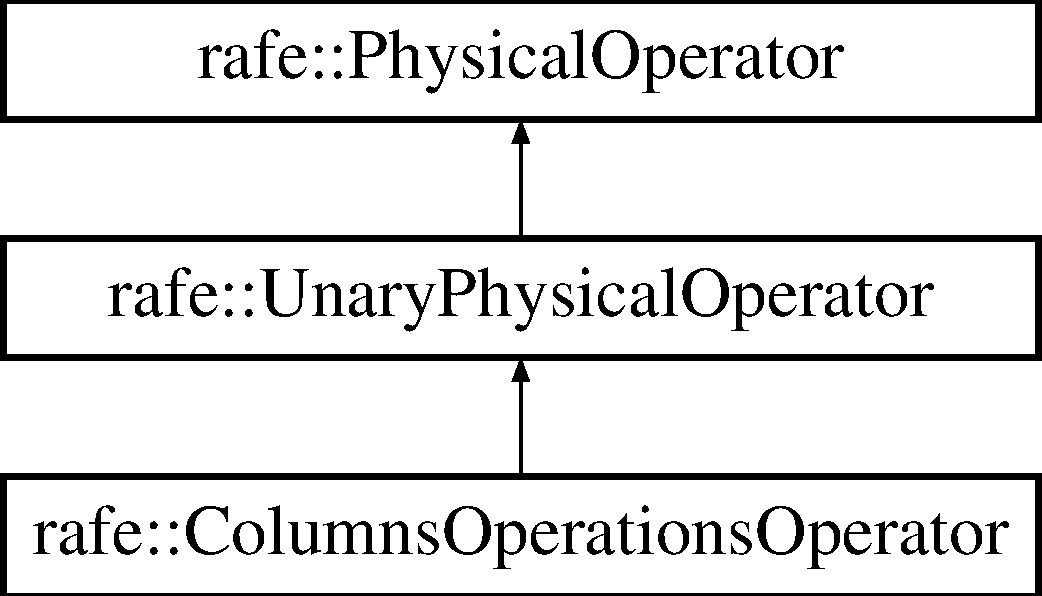
\includegraphics[height=3.000000cm]{classrafe_1_1_columns_operations_operator}
\end{center}
\end{figure}
\subsection*{Public Member Functions}
\begin{DoxyCompactItemize}
\item 
\hyperlink{classrafe_1_1_columns_operations_operator_a2fabdd215667318465dcd75d878db071}{Columns\+Operations\+Operator} (const std\+::vector$<$ \hyperlink{classrafe_1_1_column_operation}{Column\+Operation} $>$ \&\hyperlink{classrafe_1_1_columns_operations_operator_a163a3eac6eb7336bda80ba844610880c}{operations})
\item 
void \hyperlink{classrafe_1_1_columns_operations_operator_a4fd8d03b5fd03393ea72dd46f4c11504}{accept} (\hyperlink{classrafe_1_1_physical_operator_visitor}{Physical\+Operator\+Visitor} \&v)
\end{DoxyCompactItemize}
\subsection*{Public Attributes}
\begin{DoxyCompactItemize}
\item 
std\+::vector$<$ \hyperlink{classrafe_1_1_column_operation}{Column\+Operation} $>$ \hyperlink{classrafe_1_1_columns_operations_operator_a163a3eac6eb7336bda80ba844610880c}{operations}
\end{DoxyCompactItemize}


\subsection{Detailed Description}
This is extended projection operator, it eliminates certain columns and computes new ones. 

\subsection{Constructor \& Destructor Documentation}
\hypertarget{classrafe_1_1_columns_operations_operator_a2fabdd215667318465dcd75d878db071}{\index{rafe\+::\+Columns\+Operations\+Operator@{rafe\+::\+Columns\+Operations\+Operator}!Columns\+Operations\+Operator@{Columns\+Operations\+Operator}}
\index{Columns\+Operations\+Operator@{Columns\+Operations\+Operator}!rafe\+::\+Columns\+Operations\+Operator@{rafe\+::\+Columns\+Operations\+Operator}}
\subsubsection[{Columns\+Operations\+Operator}]{\setlength{\rightskip}{0pt plus 5cm}rafe\+::\+Columns\+Operations\+Operator\+::\+Columns\+Operations\+Operator (
\begin{DoxyParamCaption}
\item[{const std\+::vector$<$ {\bf Column\+Operation} $>$ \&}]{operations}
\end{DoxyParamCaption}
)}}\label{classrafe_1_1_columns_operations_operator_a2fabdd215667318465dcd75d878db071}
Creates new instance of \hyperlink{classrafe_1_1_columns_operations_operator}{Columns\+Operations\+Operator}. 
\begin{DoxyParams}{Parameters}
{\em operations} & -\/ information about output and new computed columns. \\
\hline
\end{DoxyParams}


\subsection{Member Function Documentation}
\hypertarget{classrafe_1_1_columns_operations_operator_a4fd8d03b5fd03393ea72dd46f4c11504}{\index{rafe\+::\+Columns\+Operations\+Operator@{rafe\+::\+Columns\+Operations\+Operator}!accept@{accept}}
\index{accept@{accept}!rafe\+::\+Columns\+Operations\+Operator@{rafe\+::\+Columns\+Operations\+Operator}}
\subsubsection[{accept}]{\setlength{\rightskip}{0pt plus 5cm}void rafe\+::\+Columns\+Operations\+Operator\+::accept (
\begin{DoxyParamCaption}
\item[{{\bf Physical\+Operator\+Visitor} \&}]{v}
\end{DoxyParamCaption}
)\hspace{0.3cm}{\ttfamily [virtual]}}}\label{classrafe_1_1_columns_operations_operator_a4fd8d03b5fd03393ea72dd46f4c11504}
Method for calling visit\mbox{[}node\mbox{]} on given \hyperlink{classrafe_1_1_physical_operator_visitor}{Physical\+Operator\+Visitor}. 
\begin{DoxyParams}{Parameters}
{\em v} & \hyperlink{classrafe_1_1_physical_operator_visitor}{Physical\+Operator\+Visitor}, on which to call function. \\
\hline
\end{DoxyParams}


Implements \hyperlink{classrafe_1_1_unary_physical_operator_a56a160698a78f8a0aa44e47e0804f45e}{rafe\+::\+Unary\+Physical\+Operator}.



\subsection{Member Data Documentation}
\hypertarget{classrafe_1_1_columns_operations_operator_a163a3eac6eb7336bda80ba844610880c}{\index{rafe\+::\+Columns\+Operations\+Operator@{rafe\+::\+Columns\+Operations\+Operator}!operations@{operations}}
\index{operations@{operations}!rafe\+::\+Columns\+Operations\+Operator@{rafe\+::\+Columns\+Operations\+Operator}}
\subsubsection[{operations}]{\setlength{\rightskip}{0pt plus 5cm}std\+::vector$<${\bf Column\+Operation}$>$ rafe\+::\+Columns\+Operations\+Operator\+::operations}}\label{classrafe_1_1_columns_operations_operator_a163a3eac6eb7336bda80ba844610880c}
Information about output and new computed columns. 

The documentation for this class was generated from the following files\+:\begin{DoxyCompactItemize}
\item 
C\+:/\+Users/\+Marcel/\+Documents/\+Visual Studio 2012/\+Projects/\+Relational\+Query\+Evaluator/\+Relational\+Query\+Evaluator/Physical\+Operator.\+h\item 
C\+:/\+Users/\+Marcel/\+Documents/\+Visual Studio 2012/\+Projects/\+Relational\+Query\+Evaluator/\+Relational\+Query\+Evaluator/Physical\+Operator.\+cpp\end{DoxyCompactItemize}

\hypertarget{classrafe_1_1_condition_info}{\section{rafe\+:\+:Condition\+Info Class Reference}
\label{classrafe_1_1_condition_info}\index{rafe\+::\+Condition\+Info@{rafe\+::\+Condition\+Info}}
}


{\ttfamily \#include $<$Algebra\+Visitors.\+h$>$}

\subsection*{Public Attributes}
\begin{DoxyCompactItemize}
\item 
std\+::shared\+\_\+ptr$<$ \hyperlink{classrafe_1_1_expression}{Expression} $>$ \hyperlink{classrafe_1_1_condition_info_aa64e9e78cfbd31a51647f9bdca6feb76}{condition}
\item 
std\+::set$<$ int $>$ \hyperlink{classrafe_1_1_condition_info_ab84980884b8f58e451054b22401eae41}{inputs}
\item 
Condition\+Type \hyperlink{classrafe_1_1_condition_info_a6145e30ff335f025f1a1bfa89005c1c2}{type}
\end{DoxyCompactItemize}


\subsection{Detailed Description}
Stores information about condition, its columns and condition type. 

\subsection{Member Data Documentation}
\hypertarget{classrafe_1_1_condition_info_aa64e9e78cfbd31a51647f9bdca6feb76}{\index{rafe\+::\+Condition\+Info@{rafe\+::\+Condition\+Info}!condition@{condition}}
\index{condition@{condition}!rafe\+::\+Condition\+Info@{rafe\+::\+Condition\+Info}}
\subsubsection[{condition}]{\setlength{\rightskip}{0pt plus 5cm}std\+::shared\+\_\+ptr$<${\bf Expression}$>$ rafe\+::\+Condition\+Info\+::condition}}\label{classrafe_1_1_condition_info_aa64e9e78cfbd31a51647f9bdca6feb76}
Given condition. \hypertarget{classrafe_1_1_condition_info_ab84980884b8f58e451054b22401eae41}{\index{rafe\+::\+Condition\+Info@{rafe\+::\+Condition\+Info}!inputs@{inputs}}
\index{inputs@{inputs}!rafe\+::\+Condition\+Info@{rafe\+::\+Condition\+Info}}
\subsubsection[{inputs}]{\setlength{\rightskip}{0pt plus 5cm}std\+::set$<$int$>$ rafe\+::\+Condition\+Info\+::inputs}}\label{classrafe_1_1_condition_info_ab84980884b8f58e451054b22401eae41}
Set of column identifiers. \hypertarget{classrafe_1_1_condition_info_a6145e30ff335f025f1a1bfa89005c1c2}{\index{rafe\+::\+Condition\+Info@{rafe\+::\+Condition\+Info}!type@{type}}
\index{type@{type}!rafe\+::\+Condition\+Info@{rafe\+::\+Condition\+Info}}
\subsubsection[{type}]{\setlength{\rightskip}{0pt plus 5cm}Condition\+Type rafe\+::\+Condition\+Info\+::type}}\label{classrafe_1_1_condition_info_a6145e30ff335f025f1a1bfa89005c1c2}
Condition type. 

The documentation for this class was generated from the following file\+:\begin{DoxyCompactItemize}
\item 
C\+:/\+Users/\+Marcel/\+Documents/\+Visual Studio 2012/\+Projects/\+Relational\+Query\+Evaluator/\+Relational\+Query\+Evaluator/Algebra\+Visitors.\+h\end{DoxyCompactItemize}

\hypertarget{classrafe_1_1_constant}{\section{rafe\+:\+:Constant Class Reference}
\label{classrafe_1_1_constant}\index{rafe\+::\+Constant@{rafe\+::\+Constant}}
}


{\ttfamily \#include $<$Expressions.\+h$>$}

Inheritance diagram for rafe\+:\+:Constant\+:\begin{figure}[H]
\begin{center}
\leavevmode
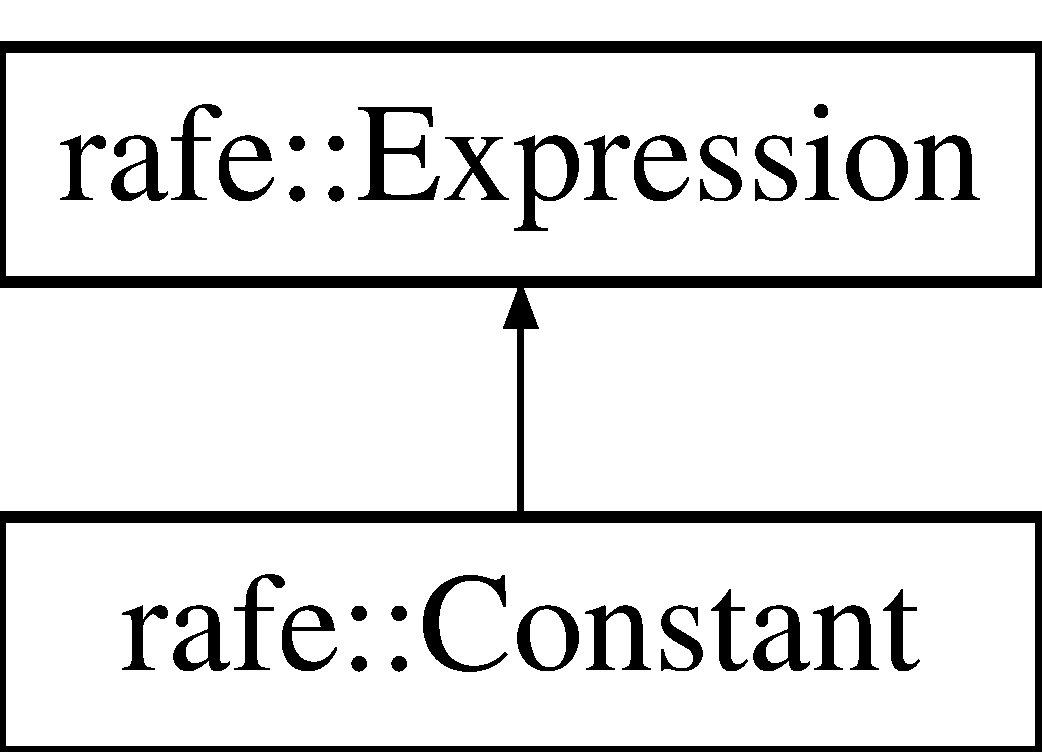
\includegraphics[height=2.000000cm]{classrafe_1_1_constant}
\end{center}
\end{figure}
\subsection*{Public Member Functions}
\begin{DoxyCompactItemize}
\item 
\hyperlink{classrafe_1_1_constant_a7eacc43b2d938e477496dc8c01b8ead3}{Constant} (D\+O\+M\+Element $\ast$node)
\item 
void \hyperlink{classrafe_1_1_constant_a867e7b315f6501bb88b33d2277b570ae}{accept} (\hyperlink{classrafe_1_1_expression_visitor_base}{Expression\+Visitor\+Base} \&v)
\item 
void \hyperlink{classrafe_1_1_constant_a5c74a0f6230626f3e49ecaae189c7a7f}{replace\+Child} (\hyperlink{classrafe_1_1_expression}{Expression} $\ast$old\+Child, std\+::shared\+\_\+ptr$<$ \hyperlink{classrafe_1_1_expression}{Expression} $>$ new\+Child)
\end{DoxyCompactItemize}
\subsection*{Public Attributes}
\begin{DoxyCompactItemize}
\item 
std\+::string \hyperlink{classrafe_1_1_constant_a22ad86666bbc772993f1f5a84dd209d7}{value}
\item 
std\+::string \hyperlink{classrafe_1_1_constant_a4fcd257fe94e9dcdf3115703904fa001}{type}
\end{DoxyCompactItemize}
\subsection*{Additional Inherited Members}


\subsection{Detailed Description}
Represents constant expression. It doesnt have any child expressions. 

\subsection{Constructor \& Destructor Documentation}
\hypertarget{classrafe_1_1_constant_a7eacc43b2d938e477496dc8c01b8ead3}{\index{rafe\+::\+Constant@{rafe\+::\+Constant}!Constant@{Constant}}
\index{Constant@{Constant}!rafe\+::\+Constant@{rafe\+::\+Constant}}
\subsubsection[{Constant}]{\setlength{\rightskip}{0pt plus 5cm}rafe\+::\+Constant\+::\+Constant (
\begin{DoxyParamCaption}
\item[{D\+O\+M\+Element $\ast$}]{node}
\end{DoxyParamCaption}
)}}\label{classrafe_1_1_constant_a7eacc43b2d938e477496dc8c01b8ead3}
Creates new instance of \hyperlink{classrafe_1_1_constant}{Constant}. 
\begin{DoxyParams}{Parameters}
{\em node} & -\/ element containing infromation about constant. \\
\hline
\end{DoxyParams}


\subsection{Member Function Documentation}
\hypertarget{classrafe_1_1_constant_a867e7b315f6501bb88b33d2277b570ae}{\index{rafe\+::\+Constant@{rafe\+::\+Constant}!accept@{accept}}
\index{accept@{accept}!rafe\+::\+Constant@{rafe\+::\+Constant}}
\subsubsection[{accept}]{\setlength{\rightskip}{0pt plus 5cm}void rafe\+::\+Constant\+::accept (
\begin{DoxyParamCaption}
\item[{{\bf Expression\+Visitor\+Base} \&}]{v}
\end{DoxyParamCaption}
)\hspace{0.3cm}{\ttfamily [virtual]}}}\label{classrafe_1_1_constant_a867e7b315f6501bb88b33d2277b570ae}
Method for calling visit\mbox{[}node\mbox{]} on given Expression\+Visitor 
\begin{DoxyParams}{Parameters}
{\em v} & Expression\+Visitor, on which to call visit function \\
\hline
\end{DoxyParams}


Implements \hyperlink{classrafe_1_1_expression_a3b2e5bae8b99ea6c9a3c92a9b949b3cd}{rafe\+::\+Expression}.

\hypertarget{classrafe_1_1_constant_a5c74a0f6230626f3e49ecaae189c7a7f}{\index{rafe\+::\+Constant@{rafe\+::\+Constant}!replace\+Child@{replace\+Child}}
\index{replace\+Child@{replace\+Child}!rafe\+::\+Constant@{rafe\+::\+Constant}}
\subsubsection[{replace\+Child}]{\setlength{\rightskip}{0pt plus 5cm}void rafe\+::\+Constant\+::replace\+Child (
\begin{DoxyParamCaption}
\item[{{\bf Expression} $\ast$}]{old\+Child, }
\item[{std\+::shared\+\_\+ptr$<$ {\bf Expression} $>$}]{new\+Child}
\end{DoxyParamCaption}
)\hspace{0.3cm}{\ttfamily [virtual]}}}\label{classrafe_1_1_constant_a5c74a0f6230626f3e49ecaae189c7a7f}
Replaces child from this class with new expression tree. 
\begin{DoxyParams}{Parameters}
{\em old\+Child} & -\/ child to replace \\
\hline
{\em new\+Child} & -\/ child to be replaced \\
\hline
\end{DoxyParams}


Implements \hyperlink{classrafe_1_1_expression_a841879e8eb85f4bb68cfeec24231a701}{rafe\+::\+Expression}.



\subsection{Member Data Documentation}
\hypertarget{classrafe_1_1_constant_a4fcd257fe94e9dcdf3115703904fa001}{\index{rafe\+::\+Constant@{rafe\+::\+Constant}!type@{type}}
\index{type@{type}!rafe\+::\+Constant@{rafe\+::\+Constant}}
\subsubsection[{type}]{\setlength{\rightskip}{0pt plus 5cm}std\+::string rafe\+::\+Constant\+::type}}\label{classrafe_1_1_constant_a4fcd257fe94e9dcdf3115703904fa001}
Stores constant type. \hypertarget{classrafe_1_1_constant_a22ad86666bbc772993f1f5a84dd209d7}{\index{rafe\+::\+Constant@{rafe\+::\+Constant}!value@{value}}
\index{value@{value}!rafe\+::\+Constant@{rafe\+::\+Constant}}
\subsubsection[{value}]{\setlength{\rightskip}{0pt plus 5cm}std\+::string rafe\+::\+Constant\+::value}}\label{classrafe_1_1_constant_a22ad86666bbc772993f1f5a84dd209d7}
Stores constant value. 

The documentation for this class was generated from the following files\+:\begin{DoxyCompactItemize}
\item 
C\+:/\+Users/\+Marcel/\+Documents/\+Visual Studio 2012/\+Projects/\+Relational\+Query\+Evaluator/\+Relational\+Query\+Evaluator/Expressions.\+h\item 
C\+:/\+Users/\+Marcel/\+Documents/\+Visual Studio 2012/\+Projects/\+Relational\+Query\+Evaluator/\+Relational\+Query\+Evaluator/Expressions.\+cpp\end{DoxyCompactItemize}

\hypertarget{classrafe_1_1_cross_join}{\section{rafe\+:\+:Cross\+Join Class Reference}
\label{classrafe_1_1_cross_join}\index{rafe\+::\+Cross\+Join@{rafe\+::\+Cross\+Join}}
}


{\ttfamily \#include $<$Physical\+Operator.\+h$>$}

Inheritance diagram for rafe\+:\+:Cross\+Join\+:\begin{figure}[H]
\begin{center}
\leavevmode
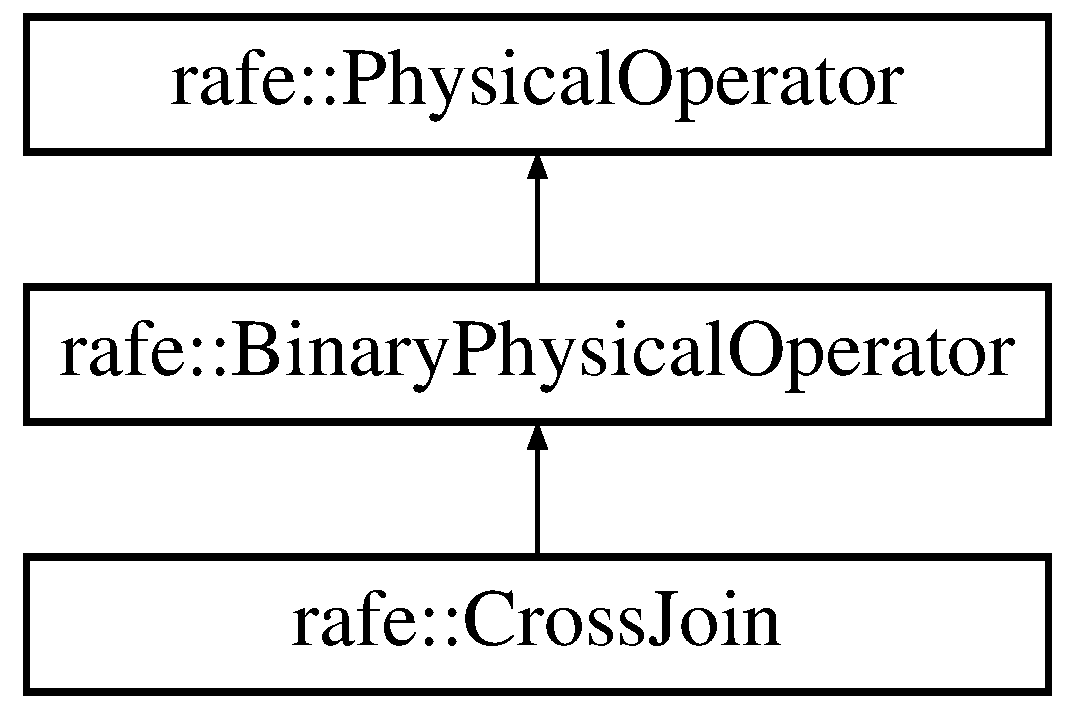
\includegraphics[height=3.000000cm]{classrafe_1_1_cross_join}
\end{center}
\end{figure}
\subsection*{Public Member Functions}
\begin{DoxyCompactItemize}
\item 
void \hyperlink{classrafe_1_1_cross_join_a3d9272caf9e1f2394f0d384f2813258a}{accept} (\hyperlink{classrafe_1_1_physical_operator_visitor}{Physical\+Operator\+Visitor} \&v)
\end{DoxyCompactItemize}
\subsection*{Additional Inherited Members}


\subsection{Detailed Description}
Represents physical cross join operator. Operator computes Cartesian product from given inputs. 

\subsection{Member Function Documentation}
\hypertarget{classrafe_1_1_cross_join_a3d9272caf9e1f2394f0d384f2813258a}{\index{rafe\+::\+Cross\+Join@{rafe\+::\+Cross\+Join}!accept@{accept}}
\index{accept@{accept}!rafe\+::\+Cross\+Join@{rafe\+::\+Cross\+Join}}
\subsubsection[{accept}]{\setlength{\rightskip}{0pt plus 5cm}void rafe\+::\+Cross\+Join\+::accept (
\begin{DoxyParamCaption}
\item[{{\bf Physical\+Operator\+Visitor} \&}]{v}
\end{DoxyParamCaption}
)\hspace{0.3cm}{\ttfamily [virtual]}}}\label{classrafe_1_1_cross_join_a3d9272caf9e1f2394f0d384f2813258a}
Method for calling visit\mbox{[}node\mbox{]} on given \hyperlink{classrafe_1_1_physical_operator_visitor}{Physical\+Operator\+Visitor}. 
\begin{DoxyParams}{Parameters}
{\em v} & \hyperlink{classrafe_1_1_physical_operator_visitor}{Physical\+Operator\+Visitor}, on which to call function. \\
\hline
\end{DoxyParams}


Implements \hyperlink{classrafe_1_1_binary_physical_operator_a58ce0a14b970b2c932254419877a2e0e}{rafe\+::\+Binary\+Physical\+Operator}.



The documentation for this class was generated from the following files\+:\begin{DoxyCompactItemize}
\item 
C\+:/\+Users/\+Marcel/\+Documents/\+Visual Studio 2012/\+Projects/\+Relational\+Query\+Evaluator/\+Relational\+Query\+Evaluator/Physical\+Operator.\+h\item 
C\+:/\+Users/\+Marcel/\+Documents/\+Visual Studio 2012/\+Projects/\+Relational\+Query\+Evaluator/\+Relational\+Query\+Evaluator/Physical\+Operator.\+cpp\end{DoxyCompactItemize}

\hypertarget{classrafe_1_1_d_o_m_parser}{\section{rafe\+:\+:D\+O\+M\+Parser Class Reference}
\label{classrafe_1_1_d_o_m_parser}\index{rafe\+::\+D\+O\+M\+Parser@{rafe\+::\+D\+O\+M\+Parser}}
}


{\ttfamily \#include $<$Xml\+Handler.\+h$>$}

Inheritance diagram for rafe\+:\+:D\+O\+M\+Parser\+:\begin{figure}[H]
\begin{center}
\leavevmode
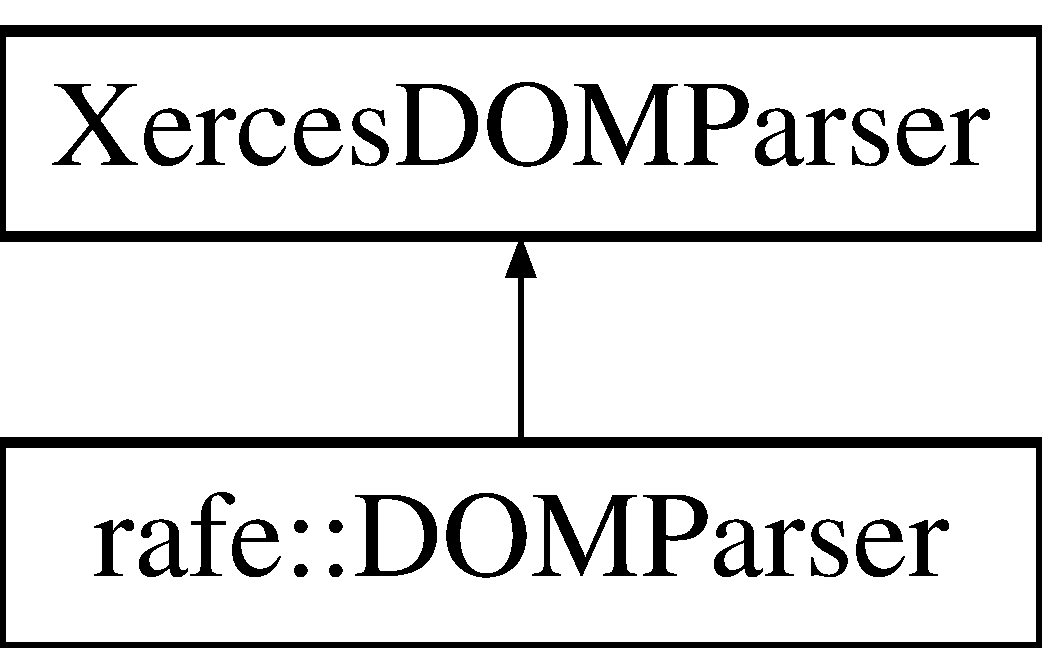
\includegraphics[height=2.000000cm]{classrafe_1_1_d_o_m_parser}
\end{center}
\end{figure}
\subsection*{Public Member Functions}
\begin{DoxyCompactItemize}
\item 
void \hyperlink{classrafe_1_1_d_o_m_parser_ac9621821b9b1030a1caee5a27454855c}{start\+Element} (const X\+M\+L\+Element\+Decl \&elem\+Decl, const unsigned int url\+Id, const X\+M\+L\+Ch $\ast$const elem\+Prefix, const Ref\+Vector\+Of$<$ X\+M\+L\+Attr $>$ \&attr\+List, const X\+M\+L\+Size\+\_\+t attr\+Count, const bool is\+Empty, const bool is\+Root)
\end{DoxyCompactItemize}


\subsection{Detailed Description}
Custom dom parser which creates dom and adds information about line number to every element. 

\subsection{Member Function Documentation}
\hypertarget{classrafe_1_1_d_o_m_parser_ac9621821b9b1030a1caee5a27454855c}{\index{rafe\+::\+D\+O\+M\+Parser@{rafe\+::\+D\+O\+M\+Parser}!start\+Element@{start\+Element}}
\index{start\+Element@{start\+Element}!rafe\+::\+D\+O\+M\+Parser@{rafe\+::\+D\+O\+M\+Parser}}
\subsubsection[{start\+Element}]{\setlength{\rightskip}{0pt plus 5cm}void rafe\+::\+D\+O\+M\+Parser\+::start\+Element (
\begin{DoxyParamCaption}
\item[{const X\+M\+L\+Element\+Decl \&}]{elem\+Decl, }
\item[{const unsigned int}]{url\+Id, }
\item[{const X\+M\+L\+Ch $\ast$const}]{elem\+Prefix, }
\item[{const Ref\+Vector\+Of$<$ X\+M\+L\+Attr $>$ \&}]{attr\+List, }
\item[{const X\+M\+L\+Size\+\_\+t}]{attr\+Count, }
\item[{const bool}]{is\+Empty, }
\item[{const bool}]{is\+Root}
\end{DoxyParamCaption}
)}}\label{classrafe_1_1_d_o_m_parser_ac9621821b9b1030a1caee5a27454855c}
Overriden method start\+Element, where parser adds information about line number to processed element. 

The documentation for this class was generated from the following files\+:\begin{DoxyCompactItemize}
\item 
C\+:/\+Users/\+Marcel/\+Documents/\+Visual Studio 2012/\+Projects/\+Relational\+Query\+Evaluator/\+Relational\+Query\+Evaluator/Xml\+Handler.\+h\item 
C\+:/\+Users/\+Marcel/\+Documents/\+Visual Studio 2012/\+Projects/\+Relational\+Query\+Evaluator/\+Relational\+Query\+Evaluator/Xml\+Handler.\+cpp\end{DoxyCompactItemize}

\hypertarget{classrafe_1_1_expression}{\section{rafe\+:\+:Expression Class Reference}
\label{classrafe_1_1_expression}\index{rafe\+::\+Expression@{rafe\+::\+Expression}}
}


{\ttfamily \#include $<$Expressions.\+h$>$}

Inheritance diagram for rafe\+:\+:Expression\+:\begin{figure}[H]
\begin{center}
\leavevmode
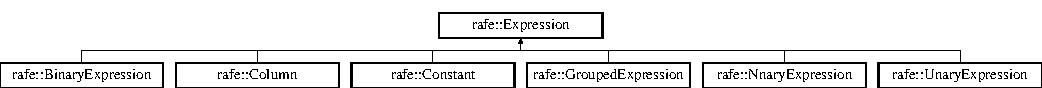
\includegraphics[height=1.166667cm]{classrafe_1_1_expression}
\end{center}
\end{figure}
\subsection*{Public Member Functions}
\begin{DoxyCompactItemize}
\item 
virtual void \hyperlink{classrafe_1_1_expression_a3b2e5bae8b99ea6c9a3c92a9b949b3cd}{accept} (\hyperlink{classrafe_1_1_expression_visitor_base}{Expression\+Visitor\+Base} \&v)=0
\item 
virtual void \hyperlink{classrafe_1_1_expression_a841879e8eb85f4bb68cfeec24231a701}{replace\+Child} (\hyperlink{classrafe_1_1_expression}{Expression} $\ast$old\+Child, std\+::shared\+\_\+ptr$<$ \hyperlink{classrafe_1_1_expression}{Expression} $>$ new\+Child)=0
\end{DoxyCompactItemize}
\subsection*{Static Public Member Functions}
\begin{DoxyCompactItemize}
\item 
static \hyperlink{classrafe_1_1_expression}{Expression} $\ast$ \hyperlink{classrafe_1_1_expression_a0a965630279f0a68f580a79fe6c5aabc}{construct\+Children} (D\+O\+M\+Element $\ast$node)
\end{DoxyCompactItemize}
\subsection*{Public Attributes}
\begin{DoxyCompactItemize}
\item 
\hyperlink{classrafe_1_1_expression}{Expression} $\ast$ \hyperlink{classrafe_1_1_expression_ae6f0ee539cc324899c34926733fe33b1}{parent}
\end{DoxyCompactItemize}


\subsection{Detailed Description}
Base class for expression in expression tree. \hyperlink{classrafe_1_1_expression}{Expression} trees are used in algebra nodes like selection, join, antijoin or column operations. 

\subsection{Member Function Documentation}
\hypertarget{classrafe_1_1_expression_a3b2e5bae8b99ea6c9a3c92a9b949b3cd}{\index{rafe\+::\+Expression@{rafe\+::\+Expression}!accept@{accept}}
\index{accept@{accept}!rafe\+::\+Expression@{rafe\+::\+Expression}}
\subsubsection[{accept}]{\setlength{\rightskip}{0pt plus 5cm}virtual void rafe\+::\+Expression\+::accept (
\begin{DoxyParamCaption}
\item[{{\bf Expression\+Visitor\+Base} \&}]{v}
\end{DoxyParamCaption}
)\hspace{0.3cm}{\ttfamily [pure virtual]}}}\label{classrafe_1_1_expression_a3b2e5bae8b99ea6c9a3c92a9b949b3cd}
Method for calling visit\mbox{[}node\mbox{]} on given Expression\+Visitor 
\begin{DoxyParams}{Parameters}
{\em v} & Expression\+Visitor, on which to call visit function \\
\hline
\end{DoxyParams}


Implemented in \hyperlink{classrafe_1_1_grouped_expression_a7f7e2cb9efd9457d80dc6365339957f6}{rafe\+::\+Grouped\+Expression}, \hyperlink{classrafe_1_1_column_addd58ca5abdbba013b744ee6a96de75d}{rafe\+::\+Column}, \hyperlink{classrafe_1_1_constant_a867e7b315f6501bb88b33d2277b570ae}{rafe\+::\+Constant}, \hyperlink{classrafe_1_1_nnary_expression_a69364332f3ee37e38901cdef923c6eeb}{rafe\+::\+Nnary\+Expression}, \hyperlink{classrafe_1_1_binary_expression_a343b5568f9fa7bf63b1f734bfed65f78}{rafe\+::\+Binary\+Expression}, and \hyperlink{classrafe_1_1_unary_expression_a04214cead0edc977169fa157fc8d13e7}{rafe\+::\+Unary\+Expression}.

\hypertarget{classrafe_1_1_expression_a0a965630279f0a68f580a79fe6c5aabc}{\index{rafe\+::\+Expression@{rafe\+::\+Expression}!construct\+Children@{construct\+Children}}
\index{construct\+Children@{construct\+Children}!rafe\+::\+Expression@{rafe\+::\+Expression}}
\subsubsection[{construct\+Children}]{\setlength{\rightskip}{0pt plus 5cm}{\bf Expression} $\ast$ rafe\+::\+Expression\+::construct\+Children (
\begin{DoxyParamCaption}
\item[{D\+O\+M\+Element $\ast$}]{node}
\end{DoxyParamCaption}
)\hspace{0.3cm}{\ttfamily [static]}}}\label{classrafe_1_1_expression_a0a965630279f0a68f580a79fe6c5aabc}
Helper function for choosing which node to conctruct from element. 
\begin{DoxyParams}{Parameters}
{\em node} & -\/ element containing information expression \\
\hline
\end{DoxyParams}
\hypertarget{classrafe_1_1_expression_a841879e8eb85f4bb68cfeec24231a701}{\index{rafe\+::\+Expression@{rafe\+::\+Expression}!replace\+Child@{replace\+Child}}
\index{replace\+Child@{replace\+Child}!rafe\+::\+Expression@{rafe\+::\+Expression}}
\subsubsection[{replace\+Child}]{\setlength{\rightskip}{0pt plus 5cm}virtual void rafe\+::\+Expression\+::replace\+Child (
\begin{DoxyParamCaption}
\item[{{\bf Expression} $\ast$}]{old\+Child, }
\item[{std\+::shared\+\_\+ptr$<$ {\bf Expression} $>$}]{new\+Child}
\end{DoxyParamCaption}
)\hspace{0.3cm}{\ttfamily [pure virtual]}}}\label{classrafe_1_1_expression_a841879e8eb85f4bb68cfeec24231a701}
Replaces child from this class with new expression tree. 
\begin{DoxyParams}{Parameters}
{\em old\+Child} & -\/ child to replace \\
\hline
{\em new\+Child} & -\/ child to be replaced \\
\hline
\end{DoxyParams}


Implemented in \hyperlink{classrafe_1_1_grouped_expression_ab770657757c0b374e4eacc8112ba9c4f}{rafe\+::\+Grouped\+Expression}, \hyperlink{classrafe_1_1_column_a420f51cd25221b94cbc0dcb7391ee950}{rafe\+::\+Column}, \hyperlink{classrafe_1_1_constant_a5c74a0f6230626f3e49ecaae189c7a7f}{rafe\+::\+Constant}, \hyperlink{classrafe_1_1_nnary_expression_a3e7adc7e9dc45caa0a6ac3919564a921}{rafe\+::\+Nnary\+Expression}, \hyperlink{classrafe_1_1_binary_expression_ac094c4a5686ded1827d12e14bdfae1c6}{rafe\+::\+Binary\+Expression}, and \hyperlink{classrafe_1_1_unary_expression_adef2ed922c3a5d6248469dc6e0b78842}{rafe\+::\+Unary\+Expression}.



\subsection{Member Data Documentation}
\hypertarget{classrafe_1_1_expression_ae6f0ee539cc324899c34926733fe33b1}{\index{rafe\+::\+Expression@{rafe\+::\+Expression}!parent@{parent}}
\index{parent@{parent}!rafe\+::\+Expression@{rafe\+::\+Expression}}
\subsubsection[{parent}]{\setlength{\rightskip}{0pt plus 5cm}{\bf Expression}$\ast$ rafe\+::\+Expression\+::parent}}\label{classrafe_1_1_expression_ae6f0ee539cc324899c34926733fe33b1}
Stores pointer on the parent in expression tree. 

The documentation for this class was generated from the following files\+:\begin{DoxyCompactItemize}
\item 
C\+:/\+Users/\+Marcel/\+Documents/\+Visual Studio 2012/\+Projects/\+Relational\+Query\+Evaluator/\+Relational\+Query\+Evaluator/Expressions.\+h\item 
C\+:/\+Users/\+Marcel/\+Documents/\+Visual Studio 2012/\+Projects/\+Relational\+Query\+Evaluator/\+Relational\+Query\+Evaluator/Expressions.\+cpp\end{DoxyCompactItemize}

\hypertarget{classrafe_1_1_expression_visitor_base}{\section{rafe\+:\+:Expression\+Visitor\+Base Class Reference}
\label{classrafe_1_1_expression_visitor_base}\index{rafe\+::\+Expression\+Visitor\+Base@{rafe\+::\+Expression\+Visitor\+Base}}
}


{\ttfamily \#include $<$Expression\+Visitors.\+h$>$}

Inheritance diagram for rafe\+:\+:Expression\+Visitor\+Base\+:\begin{figure}[H]
\begin{center}
\leavevmode
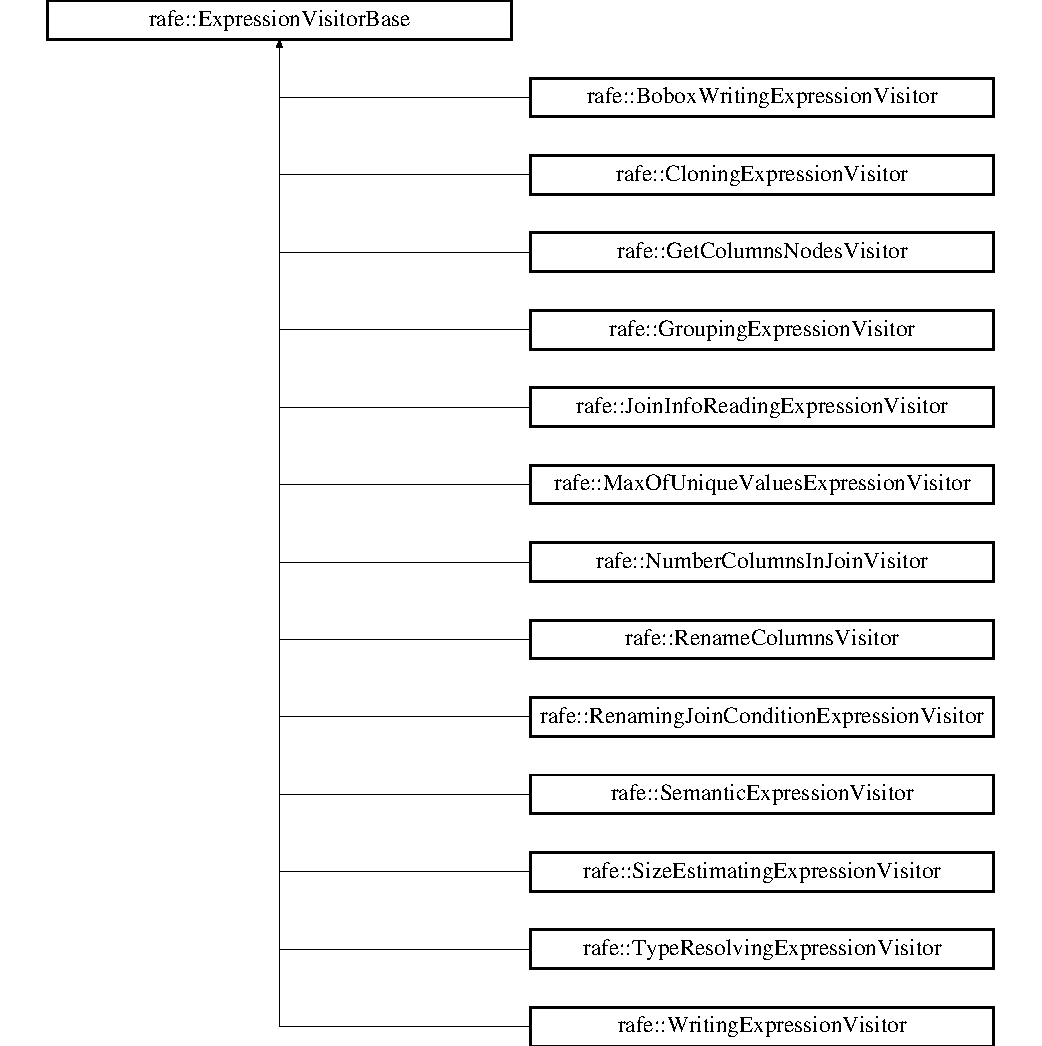
\includegraphics[height=12.000000cm]{classrafe_1_1_expression_visitor_base}
\end{center}
\end{figure}
\subsection*{Public Member Functions}
\begin{DoxyCompactItemize}
\item 
virtual void \hyperlink{classrafe_1_1_expression_visitor_base_a439348ee979dff26c30707f1ef499e8c}{visit\+Unary\+Expression} (\hyperlink{classrafe_1_1_unary_expression}{Unary\+Expression} $\ast$expression)
\item 
virtual void \hyperlink{classrafe_1_1_expression_visitor_base_a63e53276af3a22d3592f34d05ba97014}{visit\+Binary\+Expression} (\hyperlink{classrafe_1_1_binary_expression}{Binary\+Expression} $\ast$expression)
\item 
virtual void \hyperlink{classrafe_1_1_expression_visitor_base_a32f89977f780ccb8aabe5afa1fa42d45}{visit\+Nnary\+Expression} (\hyperlink{classrafe_1_1_nnary_expression}{Nnary\+Expression} $\ast$expression)
\item 
virtual void \hyperlink{classrafe_1_1_expression_visitor_base_af934111c6881f9f6c3ef3aa51425b9ff}{visit\+Constant} (\hyperlink{classrafe_1_1_constant}{Constant} $\ast$expression)
\item 
virtual void \hyperlink{classrafe_1_1_expression_visitor_base_a4eaa77bf4105d1cbdde4feb047228255}{visit\+Column} (\hyperlink{classrafe_1_1_column}{Column} $\ast$expression)
\item 
virtual void \hyperlink{classrafe_1_1_expression_visitor_base_a76226ab9d571ed7eaf80d2ed7153791c}{visit\+Grouped\+Expression} (\hyperlink{classrafe_1_1_grouped_expression}{Grouped\+Expression} $\ast$expression)
\end{DoxyCompactItemize}


\subsection{Detailed Description}
Base class for expression visitors. Every virtual method does nothing only visits node all children. 

\subsection{Member Function Documentation}
\hypertarget{classrafe_1_1_expression_visitor_base_a63e53276af3a22d3592f34d05ba97014}{\index{rafe\+::\+Expression\+Visitor\+Base@{rafe\+::\+Expression\+Visitor\+Base}!visit\+Binary\+Expression@{visit\+Binary\+Expression}}
\index{visit\+Binary\+Expression@{visit\+Binary\+Expression}!rafe\+::\+Expression\+Visitor\+Base@{rafe\+::\+Expression\+Visitor\+Base}}
\subsubsection[{visit\+Binary\+Expression}]{\setlength{\rightskip}{0pt plus 5cm}void rafe\+::\+Expression\+Visitor\+Base\+::visit\+Binary\+Expression (
\begin{DoxyParamCaption}
\item[{{\bf Binary\+Expression} $\ast$}]{expression}
\end{DoxyParamCaption}
)\hspace{0.3cm}{\ttfamily [virtual]}}}\label{classrafe_1_1_expression_visitor_base_a63e53276af3a22d3592f34d05ba97014}
Visits \hyperlink{classrafe_1_1_binary_expression}{Binary\+Expression} element. 
\begin{DoxyParams}{Parameters}
{\em expression} & visited \hyperlink{classrafe_1_1_binary_expression}{Binary\+Expression}. \\
\hline
\end{DoxyParams}


Reimplemented in \hyperlink{classrafe_1_1_cloning_expression_visitor_a021e146e191a9fce4b7b82f0c4b4efd4}{rafe\+::\+Cloning\+Expression\+Visitor}, \hyperlink{classrafe_1_1_bobox_writing_expression_visitor_a4bf6fe93d12d89e40d30ef811442e666}{rafe\+::\+Bobox\+Writing\+Expression\+Visitor}, \hyperlink{classrafe_1_1_type_resolving_expression_visitor_a3a46e7e142337f41960395c8e1fc773a}{rafe\+::\+Type\+Resolving\+Expression\+Visitor}, \hyperlink{classrafe_1_1_join_info_reading_expression_visitor_a3fe9a23de3b525cc967c0f8b1c2c81eb}{rafe\+::\+Join\+Info\+Reading\+Expression\+Visitor}, \hyperlink{classrafe_1_1_size_estimating_expression_visitor_ae6dad0b04f4eb3e201a9677124f9577c}{rafe\+::\+Size\+Estimating\+Expression\+Visitor}, \hyperlink{classrafe_1_1_grouping_expression_visitor_a5ef6febb7f733f4adcf61bc83a6d10f8}{rafe\+::\+Grouping\+Expression\+Visitor}, \hyperlink{classrafe_1_1_number_columns_in_join_visitor_a56c533c28f9948a6fcc0e8856a7b19e4}{rafe\+::\+Number\+Columns\+In\+Join\+Visitor}, and \hyperlink{classrafe_1_1_writing_expression_visitor_ab4cb67967bc57450d891a87bcebde472}{rafe\+::\+Writing\+Expression\+Visitor}.

\hypertarget{classrafe_1_1_expression_visitor_base_a4eaa77bf4105d1cbdde4feb047228255}{\index{rafe\+::\+Expression\+Visitor\+Base@{rafe\+::\+Expression\+Visitor\+Base}!visit\+Column@{visit\+Column}}
\index{visit\+Column@{visit\+Column}!rafe\+::\+Expression\+Visitor\+Base@{rafe\+::\+Expression\+Visitor\+Base}}
\subsubsection[{visit\+Column}]{\setlength{\rightskip}{0pt plus 5cm}void rafe\+::\+Expression\+Visitor\+Base\+::visit\+Column (
\begin{DoxyParamCaption}
\item[{{\bf Column} $\ast$}]{expression}
\end{DoxyParamCaption}
)\hspace{0.3cm}{\ttfamily [virtual]}}}\label{classrafe_1_1_expression_visitor_base_a4eaa77bf4105d1cbdde4feb047228255}
Visits \hyperlink{classrafe_1_1_column}{Column} element. 
\begin{DoxyParams}{Parameters}
{\em expression} & visited \hyperlink{classrafe_1_1_column}{Column}. \\
\hline
\end{DoxyParams}


Reimplemented in \hyperlink{classrafe_1_1_rename_columns_visitor_af7ca189c54c24f4460f5b79860d0149c}{rafe\+::\+Rename\+Columns\+Visitor}, \hyperlink{classrafe_1_1_cloning_expression_visitor_a0182fb9588af653201a5450935cf0b87}{rafe\+::\+Cloning\+Expression\+Visitor}, \hyperlink{classrafe_1_1_bobox_writing_expression_visitor_a7c431ef8456be3affdb17692b99d8e50}{rafe\+::\+Bobox\+Writing\+Expression\+Visitor}, \hyperlink{classrafe_1_1_type_resolving_expression_visitor_a89cc0145ce0d723da377fac1996067bf}{rafe\+::\+Type\+Resolving\+Expression\+Visitor}, \hyperlink{classrafe_1_1_max_of_unique_values_expression_visitor_af7018ac8dc1f162aa263d16e0c9f757a}{rafe\+::\+Max\+Of\+Unique\+Values\+Expression\+Visitor}, \hyperlink{classrafe_1_1_renaming_join_condition_expression_visitor_a5e8310c5df8f8f36c96958fbcee0edd3}{rafe\+::\+Renaming\+Join\+Condition\+Expression\+Visitor}, \hyperlink{classrafe_1_1_join_info_reading_expression_visitor_a791b1f98544255f24c39b77286b459d9}{rafe\+::\+Join\+Info\+Reading\+Expression\+Visitor}, \hyperlink{classrafe_1_1_semantic_expression_visitor_a605cf8d023dc621ac96d0b82d19d1b42}{rafe\+::\+Semantic\+Expression\+Visitor}, \hyperlink{classrafe_1_1_get_columns_nodes_visitor_a60dd06cf2b318397476a9eba5e32a078}{rafe\+::\+Get\+Columns\+Nodes\+Visitor}, \hyperlink{classrafe_1_1_number_columns_in_join_visitor_a0a9ea8d0e184365f7f869452e13b8a63}{rafe\+::\+Number\+Columns\+In\+Join\+Visitor}, and \hyperlink{classrafe_1_1_writing_expression_visitor_a29f80e3c4267e05e49e48f44abd8cc94}{rafe\+::\+Writing\+Expression\+Visitor}.

\hypertarget{classrafe_1_1_expression_visitor_base_af934111c6881f9f6c3ef3aa51425b9ff}{\index{rafe\+::\+Expression\+Visitor\+Base@{rafe\+::\+Expression\+Visitor\+Base}!visit\+Constant@{visit\+Constant}}
\index{visit\+Constant@{visit\+Constant}!rafe\+::\+Expression\+Visitor\+Base@{rafe\+::\+Expression\+Visitor\+Base}}
\subsubsection[{visit\+Constant}]{\setlength{\rightskip}{0pt plus 5cm}void rafe\+::\+Expression\+Visitor\+Base\+::visit\+Constant (
\begin{DoxyParamCaption}
\item[{{\bf Constant} $\ast$}]{expression}
\end{DoxyParamCaption}
)\hspace{0.3cm}{\ttfamily [virtual]}}}\label{classrafe_1_1_expression_visitor_base_af934111c6881f9f6c3ef3aa51425b9ff}
Visits \hyperlink{classrafe_1_1_constant}{Constant} element. 
\begin{DoxyParams}{Parameters}
{\em expression} & visited \hyperlink{classrafe_1_1_constant}{Constant}. \\
\hline
\end{DoxyParams}


Reimplemented in \hyperlink{classrafe_1_1_cloning_expression_visitor_a1fc965624f46b446b7836fc274962f02}{rafe\+::\+Cloning\+Expression\+Visitor}, \hyperlink{classrafe_1_1_bobox_writing_expression_visitor_a2228a1d5a64ae2ef765f5360b5eb9a30}{rafe\+::\+Bobox\+Writing\+Expression\+Visitor}, \hyperlink{classrafe_1_1_type_resolving_expression_visitor_af4d0c76b55893e462c12ce165dcb4275}{rafe\+::\+Type\+Resolving\+Expression\+Visitor}, \hyperlink{classrafe_1_1_join_info_reading_expression_visitor_aa08dee45829be99a6c6b3961c8cf081d}{rafe\+::\+Join\+Info\+Reading\+Expression\+Visitor}, and \hyperlink{classrafe_1_1_writing_expression_visitor_a30b82d54f29dc7a1ffc4ba67581dc680}{rafe\+::\+Writing\+Expression\+Visitor}.

\hypertarget{classrafe_1_1_expression_visitor_base_a76226ab9d571ed7eaf80d2ed7153791c}{\index{rafe\+::\+Expression\+Visitor\+Base@{rafe\+::\+Expression\+Visitor\+Base}!visit\+Grouped\+Expression@{visit\+Grouped\+Expression}}
\index{visit\+Grouped\+Expression@{visit\+Grouped\+Expression}!rafe\+::\+Expression\+Visitor\+Base@{rafe\+::\+Expression\+Visitor\+Base}}
\subsubsection[{visit\+Grouped\+Expression}]{\setlength{\rightskip}{0pt plus 5cm}void rafe\+::\+Expression\+Visitor\+Base\+::visit\+Grouped\+Expression (
\begin{DoxyParamCaption}
\item[{{\bf Grouped\+Expression} $\ast$}]{expression}
\end{DoxyParamCaption}
)\hspace{0.3cm}{\ttfamily [virtual]}}}\label{classrafe_1_1_expression_visitor_base_a76226ab9d571ed7eaf80d2ed7153791c}
Visits \hyperlink{classrafe_1_1_grouped_expression}{Grouped\+Expression} element. 
\begin{DoxyParams}{Parameters}
{\em expression} & visited \hyperlink{classrafe_1_1_grouped_expression}{Grouped\+Expression}. \\
\hline
\end{DoxyParams}


Reimplemented in \hyperlink{classrafe_1_1_cloning_expression_visitor_a54f879bde3c538a907782a32e1eee492}{rafe\+::\+Cloning\+Expression\+Visitor}, \hyperlink{classrafe_1_1_bobox_writing_expression_visitor_a5c00ebe39e50c4e6ad35f35a1248ef8e}{rafe\+::\+Bobox\+Writing\+Expression\+Visitor}, \hyperlink{classrafe_1_1_type_resolving_expression_visitor_a08c282c4872c03ee57f361e1f0843566}{rafe\+::\+Type\+Resolving\+Expression\+Visitor}, \hyperlink{classrafe_1_1_join_info_reading_expression_visitor_acfd9c7c62dfac50b0ac6d1c314f7f395}{rafe\+::\+Join\+Info\+Reading\+Expression\+Visitor}, \hyperlink{classrafe_1_1_size_estimating_expression_visitor_a56a98bed6c990f2a71ab18ca59ded1eb}{rafe\+::\+Size\+Estimating\+Expression\+Visitor}, and \hyperlink{classrafe_1_1_writing_expression_visitor_a4e57643ee4d25bc3a75e8a045524329d}{rafe\+::\+Writing\+Expression\+Visitor}.

\hypertarget{classrafe_1_1_expression_visitor_base_a32f89977f780ccb8aabe5afa1fa42d45}{\index{rafe\+::\+Expression\+Visitor\+Base@{rafe\+::\+Expression\+Visitor\+Base}!visit\+Nnary\+Expression@{visit\+Nnary\+Expression}}
\index{visit\+Nnary\+Expression@{visit\+Nnary\+Expression}!rafe\+::\+Expression\+Visitor\+Base@{rafe\+::\+Expression\+Visitor\+Base}}
\subsubsection[{visit\+Nnary\+Expression}]{\setlength{\rightskip}{0pt plus 5cm}void rafe\+::\+Expression\+Visitor\+Base\+::visit\+Nnary\+Expression (
\begin{DoxyParamCaption}
\item[{{\bf Nnary\+Expression} $\ast$}]{expression}
\end{DoxyParamCaption}
)\hspace{0.3cm}{\ttfamily [virtual]}}}\label{classrafe_1_1_expression_visitor_base_a32f89977f780ccb8aabe5afa1fa42d45}
Visits \hyperlink{classrafe_1_1_nnary_expression}{Nnary\+Expression} element. 
\begin{DoxyParams}{Parameters}
{\em expression} & visited \hyperlink{classrafe_1_1_nnary_expression}{Nnary\+Expression}. \\
\hline
\end{DoxyParams}


Reimplemented in \hyperlink{classrafe_1_1_cloning_expression_visitor_ad40e5659edc1098b8465ea64eaeea7cd}{rafe\+::\+Cloning\+Expression\+Visitor}, \hyperlink{classrafe_1_1_bobox_writing_expression_visitor_a4d004f836ea9b45c8a08de32cb72bdb3}{rafe\+::\+Bobox\+Writing\+Expression\+Visitor}, \hyperlink{classrafe_1_1_type_resolving_expression_visitor_a78e0e725ec8c3add1156949df6a86252}{rafe\+::\+Type\+Resolving\+Expression\+Visitor}, \hyperlink{classrafe_1_1_join_info_reading_expression_visitor_a57a8dedf4fa06ff27c71cf36ee7a4b3b}{rafe\+::\+Join\+Info\+Reading\+Expression\+Visitor}, \hyperlink{classrafe_1_1_size_estimating_expression_visitor_a1f1f7587679efcba503a794558980c1a}{rafe\+::\+Size\+Estimating\+Expression\+Visitor}, and \hyperlink{classrafe_1_1_writing_expression_visitor_a7b7d99dfe5f882b1282b451909838929}{rafe\+::\+Writing\+Expression\+Visitor}.

\hypertarget{classrafe_1_1_expression_visitor_base_a439348ee979dff26c30707f1ef499e8c}{\index{rafe\+::\+Expression\+Visitor\+Base@{rafe\+::\+Expression\+Visitor\+Base}!visit\+Unary\+Expression@{visit\+Unary\+Expression}}
\index{visit\+Unary\+Expression@{visit\+Unary\+Expression}!rafe\+::\+Expression\+Visitor\+Base@{rafe\+::\+Expression\+Visitor\+Base}}
\subsubsection[{visit\+Unary\+Expression}]{\setlength{\rightskip}{0pt plus 5cm}void rafe\+::\+Expression\+Visitor\+Base\+::visit\+Unary\+Expression (
\begin{DoxyParamCaption}
\item[{{\bf Unary\+Expression} $\ast$}]{expression}
\end{DoxyParamCaption}
)\hspace{0.3cm}{\ttfamily [virtual]}}}\label{classrafe_1_1_expression_visitor_base_a439348ee979dff26c30707f1ef499e8c}
Visits \hyperlink{classrafe_1_1_unary_expression}{Unary\+Expression} element. 
\begin{DoxyParams}{Parameters}
{\em expression} & visited \hyperlink{classrafe_1_1_unary_expression}{Unary\+Expression}. \\
\hline
\end{DoxyParams}


Reimplemented in \hyperlink{classrafe_1_1_cloning_expression_visitor_a3b71db5c48bc772a4b8bf52a79ff1e83}{rafe\+::\+Cloning\+Expression\+Visitor}, \hyperlink{classrafe_1_1_bobox_writing_expression_visitor_aa2ebbdd925b785deb29d0ee1f326d917}{rafe\+::\+Bobox\+Writing\+Expression\+Visitor}, \hyperlink{classrafe_1_1_type_resolving_expression_visitor_ae14bae4b659f64615fc38c996828e19d}{rafe\+::\+Type\+Resolving\+Expression\+Visitor}, \hyperlink{classrafe_1_1_join_info_reading_expression_visitor_a27ebab51d1b63683004f2ec45d15869f}{rafe\+::\+Join\+Info\+Reading\+Expression\+Visitor}, \hyperlink{classrafe_1_1_size_estimating_expression_visitor_aafce8eb508a6b022d4247f14680ba472}{rafe\+::\+Size\+Estimating\+Expression\+Visitor}, and \hyperlink{classrafe_1_1_writing_expression_visitor_af95c4c680abc9663fbc5ca7e0e419723}{rafe\+::\+Writing\+Expression\+Visitor}.



The documentation for this class was generated from the following files\+:\begin{DoxyCompactItemize}
\item 
C\+:/\+Users/\+Marcel/\+Documents/\+Visual Studio 2012/\+Projects/\+Relational\+Query\+Evaluator/\+Relational\+Query\+Evaluator/Expression\+Visitors.\+h\item 
C\+:/\+Users/\+Marcel/\+Documents/\+Visual Studio 2012/\+Projects/\+Relational\+Query\+Evaluator/\+Relational\+Query\+Evaluator/Expression\+Visitors.\+cpp\end{DoxyCompactItemize}

\hypertarget{classrafe_1_1_filter}{\section{rafe\+:\+:Filter Class Reference}
\label{classrafe_1_1_filter}\index{rafe\+::\+Filter@{rafe\+::\+Filter}}
}


{\ttfamily \#include $<$Physical\+Operator.\+h$>$}

Inheritance diagram for rafe\+:\+:Filter\+:\begin{figure}[H]
\begin{center}
\leavevmode
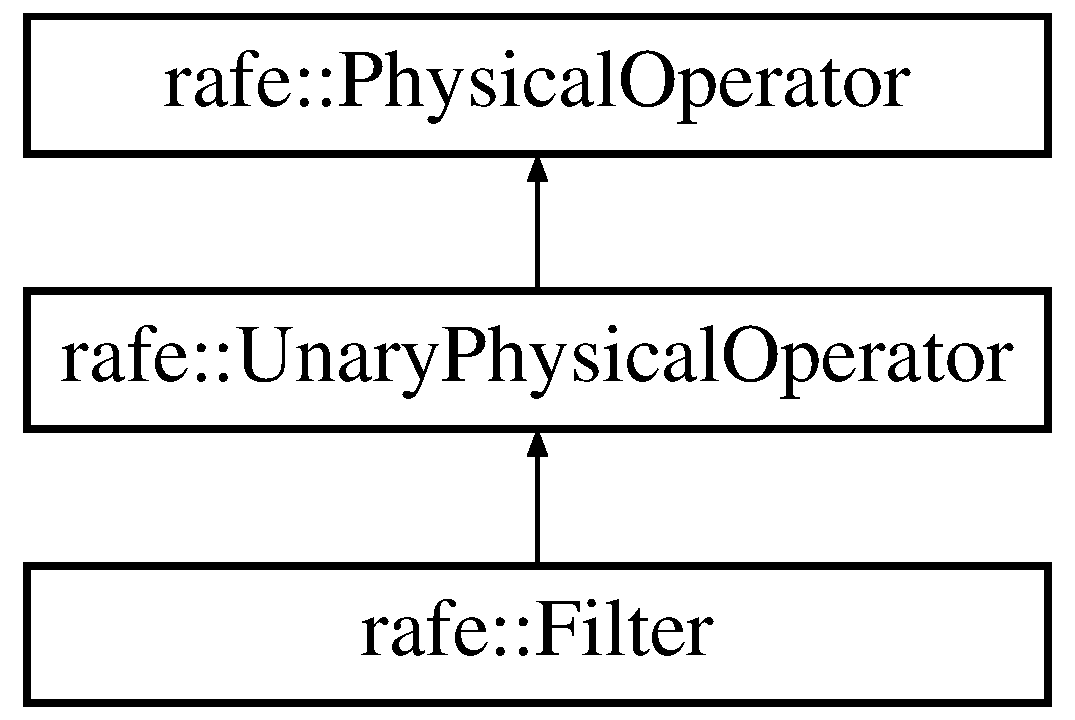
\includegraphics[height=3.000000cm]{classrafe_1_1_filter}
\end{center}
\end{figure}
\subsection*{Public Member Functions}
\begin{DoxyCompactItemize}
\item 
\hyperlink{classrafe_1_1_filter_af4f33192eef0626cf16fc9cb51b3e3de}{Filter} (const std\+::shared\+\_\+ptr$<$ \hyperlink{classrafe_1_1_expression}{Expression} $>$ \&\hyperlink{classrafe_1_1_filter_ac57844e611bd2d1951d1d4089135ddb9}{condition})
\item 
void \hyperlink{classrafe_1_1_filter_a27d15fd98afe3c03f05f5a4c5846b2a6}{accept} (\hyperlink{classrafe_1_1_physical_operator_visitor}{Physical\+Operator\+Visitor} \&v)
\end{DoxyCompactItemize}
\subsection*{Public Attributes}
\begin{DoxyCompactItemize}
\item 
std\+::shared\+\_\+ptr$<$ \hyperlink{classrafe_1_1_expression}{Expression} $>$ \hyperlink{classrafe_1_1_filter_ac57844e611bd2d1951d1d4089135ddb9}{condition}
\end{DoxyCompactItemize}


\subsection{Detailed Description}
Class representing filter physical algorithm. Operator filters given rows and output only rows satisfying condition. Output does not have to be sorted same way as input. 

\subsection{Constructor \& Destructor Documentation}
\hypertarget{classrafe_1_1_filter_af4f33192eef0626cf16fc9cb51b3e3de}{\index{rafe\+::\+Filter@{rafe\+::\+Filter}!Filter@{Filter}}
\index{Filter@{Filter}!rafe\+::\+Filter@{rafe\+::\+Filter}}
\subsubsection[{Filter}]{\setlength{\rightskip}{0pt plus 5cm}rafe\+::\+Filter\+::\+Filter (
\begin{DoxyParamCaption}
\item[{const std\+::shared\+\_\+ptr$<$ {\bf Expression} $>$ \&}]{condition}
\end{DoxyParamCaption}
)}}\label{classrafe_1_1_filter_af4f33192eef0626cf16fc9cb51b3e3de}
Creates new instance of \hyperlink{classrafe_1_1_filter}{Filter}. 
\begin{DoxyParams}{Parameters}
{\em condition} & -\/ filter condition. \\
\hline
\end{DoxyParams}


\subsection{Member Function Documentation}
\hypertarget{classrafe_1_1_filter_a27d15fd98afe3c03f05f5a4c5846b2a6}{\index{rafe\+::\+Filter@{rafe\+::\+Filter}!accept@{accept}}
\index{accept@{accept}!rafe\+::\+Filter@{rafe\+::\+Filter}}
\subsubsection[{accept}]{\setlength{\rightskip}{0pt plus 5cm}void rafe\+::\+Filter\+::accept (
\begin{DoxyParamCaption}
\item[{{\bf Physical\+Operator\+Visitor} \&}]{v}
\end{DoxyParamCaption}
)\hspace{0.3cm}{\ttfamily [virtual]}}}\label{classrafe_1_1_filter_a27d15fd98afe3c03f05f5a4c5846b2a6}
Method for calling visit\mbox{[}node\mbox{]} on given \hyperlink{classrafe_1_1_physical_operator_visitor}{Physical\+Operator\+Visitor}. 
\begin{DoxyParams}{Parameters}
{\em v} & \hyperlink{classrafe_1_1_physical_operator_visitor}{Physical\+Operator\+Visitor}, on which to call function. \\
\hline
\end{DoxyParams}


Implements \hyperlink{classrafe_1_1_unary_physical_operator_a56a160698a78f8a0aa44e47e0804f45e}{rafe\+::\+Unary\+Physical\+Operator}.



\subsection{Member Data Documentation}
\hypertarget{classrafe_1_1_filter_ac57844e611bd2d1951d1d4089135ddb9}{\index{rafe\+::\+Filter@{rafe\+::\+Filter}!condition@{condition}}
\index{condition@{condition}!rafe\+::\+Filter@{rafe\+::\+Filter}}
\subsubsection[{condition}]{\setlength{\rightskip}{0pt plus 5cm}std\+::shared\+\_\+ptr$<${\bf Expression}$>$ rafe\+::\+Filter\+::condition}}\label{classrafe_1_1_filter_ac57844e611bd2d1951d1d4089135ddb9}
Condition for filtering relation. 

The documentation for this class was generated from the following files\+:\begin{DoxyCompactItemize}
\item 
C\+:/\+Users/\+Marcel/\+Documents/\+Visual Studio 2012/\+Projects/\+Relational\+Query\+Evaluator/\+Relational\+Query\+Evaluator/Physical\+Operator.\+h\item 
C\+:/\+Users/\+Marcel/\+Documents/\+Visual Studio 2012/\+Projects/\+Relational\+Query\+Evaluator/\+Relational\+Query\+Evaluator/Physical\+Operator.\+cpp\end{DoxyCompactItemize}

\hypertarget{classrafe_1_1_filter_keeping_order}{\section{rafe\+:\+:Filter\+Keeping\+Order Class Reference}
\label{classrafe_1_1_filter_keeping_order}\index{rafe\+::\+Filter\+Keeping\+Order@{rafe\+::\+Filter\+Keeping\+Order}}
}


{\ttfamily \#include $<$Physical\+Operator.\+h$>$}

Inheritance diagram for rafe\+:\+:Filter\+Keeping\+Order\+:\begin{figure}[H]
\begin{center}
\leavevmode
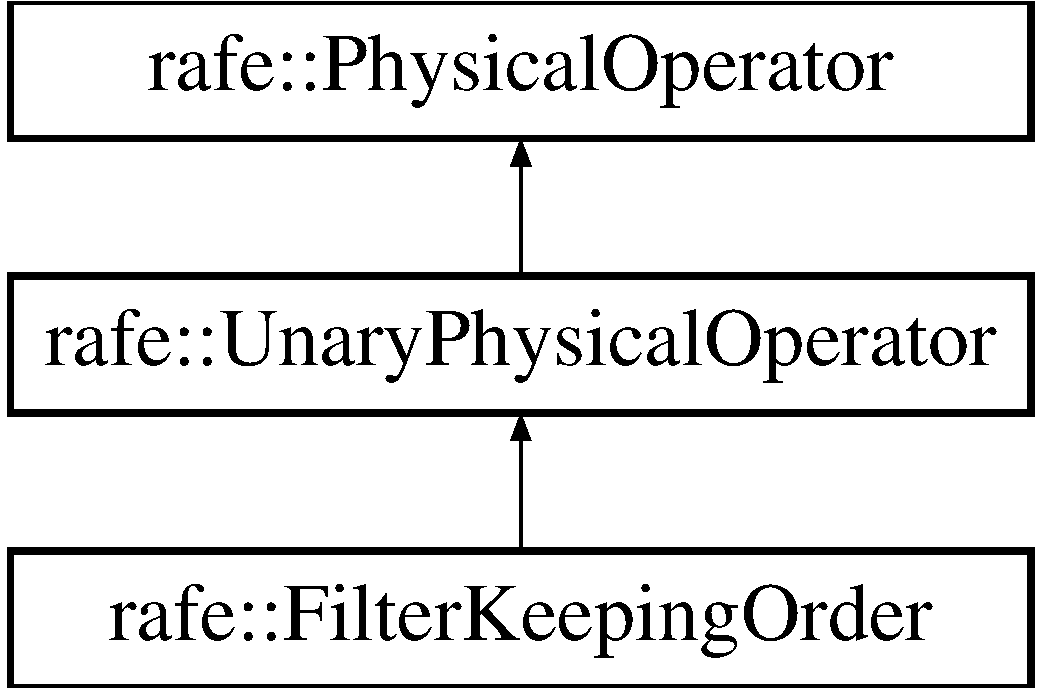
\includegraphics[height=3.000000cm]{classrafe_1_1_filter_keeping_order}
\end{center}
\end{figure}
\subsection*{Public Member Functions}
\begin{DoxyCompactItemize}
\item 
\hyperlink{classrafe_1_1_filter_keeping_order_a898792d39b2f5c7870111f859aecf0a4}{Filter\+Keeping\+Order} (const std\+::shared\+\_\+ptr$<$ \hyperlink{classrafe_1_1_expression}{Expression} $>$ \&\hyperlink{classrafe_1_1_filter_keeping_order_a94eced2ee1d9bcd744315548476fd292}{condition})
\item 
void \hyperlink{classrafe_1_1_filter_keeping_order_afde88521596d848cde18c0468aeb6062}{accept} (\hyperlink{classrafe_1_1_physical_operator_visitor}{Physical\+Operator\+Visitor} \&v)
\end{DoxyCompactItemize}
\subsection*{Public Attributes}
\begin{DoxyCompactItemize}
\item 
std\+::shared\+\_\+ptr$<$ \hyperlink{classrafe_1_1_expression}{Expression} $>$ \hyperlink{classrafe_1_1_filter_keeping_order_a94eced2ee1d9bcd744315548476fd292}{condition}
\end{DoxyCompactItemize}


\subsection{Detailed Description}
Class representing filter physical algorithm. Operator filters given rows and outputs only rows satisfying condition. Output has to be sorted the same way as input. 

\subsection{Constructor \& Destructor Documentation}
\hypertarget{classrafe_1_1_filter_keeping_order_a898792d39b2f5c7870111f859aecf0a4}{\index{rafe\+::\+Filter\+Keeping\+Order@{rafe\+::\+Filter\+Keeping\+Order}!Filter\+Keeping\+Order@{Filter\+Keeping\+Order}}
\index{Filter\+Keeping\+Order@{Filter\+Keeping\+Order}!rafe\+::\+Filter\+Keeping\+Order@{rafe\+::\+Filter\+Keeping\+Order}}
\subsubsection[{Filter\+Keeping\+Order}]{\setlength{\rightskip}{0pt plus 5cm}rafe\+::\+Filter\+Keeping\+Order\+::\+Filter\+Keeping\+Order (
\begin{DoxyParamCaption}
\item[{const std\+::shared\+\_\+ptr$<$ {\bf Expression} $>$ \&}]{condition}
\end{DoxyParamCaption}
)}}\label{classrafe_1_1_filter_keeping_order_a898792d39b2f5c7870111f859aecf0a4}
Creates new instance of \hyperlink{classrafe_1_1_filter_keeping_order}{Filter\+Keeping\+Order}. 
\begin{DoxyParams}{Parameters}
{\em condition} & -\/ filter condition. \\
\hline
\end{DoxyParams}


\subsection{Member Function Documentation}
\hypertarget{classrafe_1_1_filter_keeping_order_afde88521596d848cde18c0468aeb6062}{\index{rafe\+::\+Filter\+Keeping\+Order@{rafe\+::\+Filter\+Keeping\+Order}!accept@{accept}}
\index{accept@{accept}!rafe\+::\+Filter\+Keeping\+Order@{rafe\+::\+Filter\+Keeping\+Order}}
\subsubsection[{accept}]{\setlength{\rightskip}{0pt plus 5cm}void rafe\+::\+Filter\+Keeping\+Order\+::accept (
\begin{DoxyParamCaption}
\item[{{\bf Physical\+Operator\+Visitor} \&}]{v}
\end{DoxyParamCaption}
)\hspace{0.3cm}{\ttfamily [virtual]}}}\label{classrafe_1_1_filter_keeping_order_afde88521596d848cde18c0468aeb6062}
Method for calling visit\mbox{[}node\mbox{]} on given \hyperlink{classrafe_1_1_physical_operator_visitor}{Physical\+Operator\+Visitor}. 
\begin{DoxyParams}{Parameters}
{\em v} & \hyperlink{classrafe_1_1_physical_operator_visitor}{Physical\+Operator\+Visitor}, on which to call function. \\
\hline
\end{DoxyParams}


Implements \hyperlink{classrafe_1_1_unary_physical_operator_a56a160698a78f8a0aa44e47e0804f45e}{rafe\+::\+Unary\+Physical\+Operator}.



\subsection{Member Data Documentation}
\hypertarget{classrafe_1_1_filter_keeping_order_a94eced2ee1d9bcd744315548476fd292}{\index{rafe\+::\+Filter\+Keeping\+Order@{rafe\+::\+Filter\+Keeping\+Order}!condition@{condition}}
\index{condition@{condition}!rafe\+::\+Filter\+Keeping\+Order@{rafe\+::\+Filter\+Keeping\+Order}}
\subsubsection[{condition}]{\setlength{\rightskip}{0pt plus 5cm}std\+::shared\+\_\+ptr$<${\bf Expression}$>$ rafe\+::\+Filter\+Keeping\+Order\+::condition}}\label{classrafe_1_1_filter_keeping_order_a94eced2ee1d9bcd744315548476fd292}
Condition for filtering relation. 

The documentation for this class was generated from the following files\+:\begin{DoxyCompactItemize}
\item 
C\+:/\+Users/\+Marcel/\+Documents/\+Visual Studio 2012/\+Projects/\+Relational\+Query\+Evaluator/\+Relational\+Query\+Evaluator/Physical\+Operator.\+h\item 
C\+:/\+Users/\+Marcel/\+Documents/\+Visual Studio 2012/\+Projects/\+Relational\+Query\+Evaluator/\+Relational\+Query\+Evaluator/Physical\+Operator.\+cpp\end{DoxyCompactItemize}

\hypertarget{classrafe_1_1_get_columns_nodes_visitor}{\section{rafe\+:\+:Get\+Columns\+Nodes\+Visitor Class Reference}
\label{classrafe_1_1_get_columns_nodes_visitor}\index{rafe\+::\+Get\+Columns\+Nodes\+Visitor@{rafe\+::\+Get\+Columns\+Nodes\+Visitor}}
}


{\ttfamily \#include $<$Expression\+Visitors.\+h$>$}

Inheritance diagram for rafe\+:\+:Get\+Columns\+Nodes\+Visitor\+:\begin{figure}[H]
\begin{center}
\leavevmode
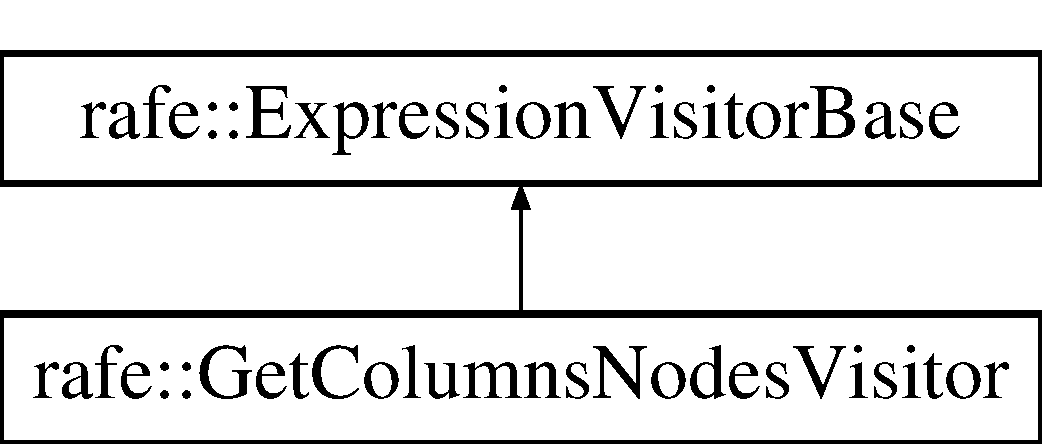
\includegraphics[height=2.000000cm]{classrafe_1_1_get_columns_nodes_visitor}
\end{center}
\end{figure}
\subsection*{Public Member Functions}
\begin{DoxyCompactItemize}
\item 
void \hyperlink{classrafe_1_1_get_columns_nodes_visitor_a60dd06cf2b318397476a9eba5e32a078}{visit\+Column} (\hyperlink{classrafe_1_1_column}{Column} $\ast$expression)
\end{DoxyCompactItemize}
\subsection*{Public Attributes}
\begin{DoxyCompactItemize}
\item 
std\+::vector$<$ \hyperlink{classrafe_1_1_column}{Column} $\ast$ $>$ \hyperlink{classrafe_1_1_get_columns_nodes_visitor_a33e85438a4b6d2474edb7ba51732c773}{nodes}
\end{DoxyCompactItemize}


\subsection{Detailed Description}
Visitor, which stores pointer of every column into vector. This visitor does not change expression tree. 

\subsection{Member Function Documentation}
\hypertarget{classrafe_1_1_get_columns_nodes_visitor_a60dd06cf2b318397476a9eba5e32a078}{\index{rafe\+::\+Get\+Columns\+Nodes\+Visitor@{rafe\+::\+Get\+Columns\+Nodes\+Visitor}!visit\+Column@{visit\+Column}}
\index{visit\+Column@{visit\+Column}!rafe\+::\+Get\+Columns\+Nodes\+Visitor@{rafe\+::\+Get\+Columns\+Nodes\+Visitor}}
\subsubsection[{visit\+Column}]{\setlength{\rightskip}{0pt plus 5cm}void rafe\+::\+Get\+Columns\+Nodes\+Visitor\+::visit\+Column (
\begin{DoxyParamCaption}
\item[{{\bf Column} $\ast$}]{expression}
\end{DoxyParamCaption}
)\hspace{0.3cm}{\ttfamily [virtual]}}}\label{classrafe_1_1_get_columns_nodes_visitor_a60dd06cf2b318397476a9eba5e32a078}
Visits \hyperlink{classrafe_1_1_column}{Column} node. 
\begin{DoxyParams}{Parameters}
{\em expression} & visited \hyperlink{classrafe_1_1_column}{Column}. \\
\hline
\end{DoxyParams}


Reimplemented from \hyperlink{classrafe_1_1_expression_visitor_base_a4eaa77bf4105d1cbdde4feb047228255}{rafe\+::\+Expression\+Visitor\+Base}.



\subsection{Member Data Documentation}
\hypertarget{classrafe_1_1_get_columns_nodes_visitor_a33e85438a4b6d2474edb7ba51732c773}{\index{rafe\+::\+Get\+Columns\+Nodes\+Visitor@{rafe\+::\+Get\+Columns\+Nodes\+Visitor}!nodes@{nodes}}
\index{nodes@{nodes}!rafe\+::\+Get\+Columns\+Nodes\+Visitor@{rafe\+::\+Get\+Columns\+Nodes\+Visitor}}
\subsubsection[{nodes}]{\setlength{\rightskip}{0pt plus 5cm}std\+::vector$<${\bf Column} $\ast$$>$ rafe\+::\+Get\+Columns\+Nodes\+Visitor\+::nodes}}\label{classrafe_1_1_get_columns_nodes_visitor_a33e85438a4b6d2474edb7ba51732c773}
Vector for saving column pointers. 

The documentation for this class was generated from the following files\+:\begin{DoxyCompactItemize}
\item 
C\+:/\+Users/\+Marcel/\+Documents/\+Visual Studio 2012/\+Projects/\+Relational\+Query\+Evaluator/\+Relational\+Query\+Evaluator/Expression\+Visitors.\+h\item 
C\+:/\+Users/\+Marcel/\+Documents/\+Visual Studio 2012/\+Projects/\+Relational\+Query\+Evaluator/\+Relational\+Query\+Evaluator/Expression\+Visitors.\+cpp\end{DoxyCompactItemize}

\hypertarget{classrafe_1_1_graph_drawing_visitor}{\section{rafe\+:\+:Graph\+Drawing\+Visitor Class Reference}
\label{classrafe_1_1_graph_drawing_visitor}\index{rafe\+::\+Graph\+Drawing\+Visitor@{rafe\+::\+Graph\+Drawing\+Visitor}}
}


{\ttfamily \#include $<$Algebra\+Visitors.\+h$>$}

Inheritance diagram for rafe\+:\+:Graph\+Drawing\+Visitor\+:\begin{figure}[H]
\begin{center}
\leavevmode
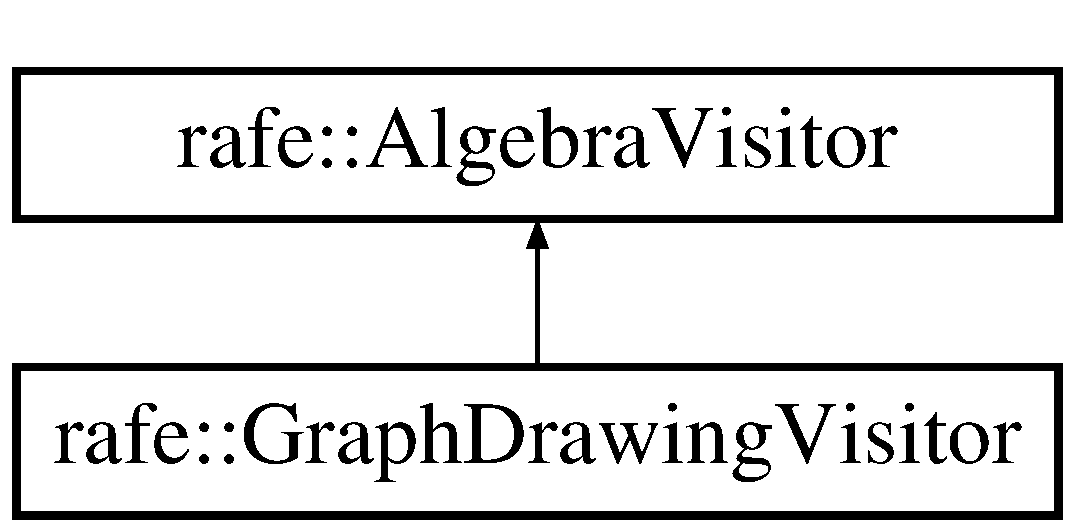
\includegraphics[height=2.000000cm]{classrafe_1_1_graph_drawing_visitor}
\end{center}
\end{figure}
\subsection*{Public Member Functions}
\begin{DoxyCompactItemize}
\item 
\hyperlink{classrafe_1_1_graph_drawing_visitor_a98fc0486336c9673c7c5eac940724ae5}{Graph\+Drawing\+Visitor} ()
\item 
void \hyperlink{classrafe_1_1_graph_drawing_visitor_a5ba892e7e9400af6d1d2f89a896babd8}{visit\+Sort} (\hyperlink{classrafe_1_1_sort}{Sort} $\ast$node)
\item 
void \hyperlink{classrafe_1_1_graph_drawing_visitor_aad5e1614a18f3d7aed5933775f614abf}{visit\+Group} (\hyperlink{classrafe_1_1_group}{Group} $\ast$node)
\item 
void \hyperlink{classrafe_1_1_graph_drawing_visitor_af5badeaa3070842bac2bad0e5bc38092}{visit\+Table} (\hyperlink{classrafe_1_1_table}{Table} $\ast$node)
\item 
void \hyperlink{classrafe_1_1_graph_drawing_visitor_a9933ed338ece545335fbad4052bf0c13}{visit\+Column\+Operations} (\hyperlink{classrafe_1_1_column_operations}{Column\+Operations} $\ast$node)
\item 
void \hyperlink{classrafe_1_1_graph_drawing_visitor_a01be2fcea00f7b0d7d70fa3dd168156c}{visit\+Selection} (\hyperlink{classrafe_1_1_selection}{Selection} $\ast$node)
\item 
void \hyperlink{classrafe_1_1_graph_drawing_visitor_abcf9e0f8c7a305923282701a17f56a8e}{visit\+Join} (\hyperlink{classrafe_1_1_join}{Join} $\ast$node)
\item 
void \hyperlink{classrafe_1_1_graph_drawing_visitor_ad21a6c42f42490a47ebb0b858a34f527}{visit\+Anti\+Join} (\hyperlink{classrafe_1_1_anti_join}{Anti\+Join} $\ast$node)
\item 
void \hyperlink{classrafe_1_1_graph_drawing_visitor_a093a7d242525ae764e2790ea06c74a9e}{visit\+Union} (\hyperlink{classrafe_1_1_union}{Union} $\ast$node)
\item 
void \hyperlink{classrafe_1_1_graph_drawing_visitor_a71b14af8909a3fe79c117ee8c8580352}{visit\+Grouped\+Join} (\hyperlink{classrafe_1_1_grouped_join}{Grouped\+Join} $\ast$node)
\end{DoxyCompactItemize}
\subsection*{Public Attributes}
\begin{DoxyCompactItemize}
\item 
std\+::string \hyperlink{classrafe_1_1_graph_drawing_visitor_a943dc1e93020b9adaa1ca6eff5c73bdd}{result}
\item 
int \hyperlink{classrafe_1_1_graph_drawing_visitor_a826fb63b5690180f6cf3c1f7fd0300b4}{node\+Counter}
\end{DoxyCompactItemize}
\subsection*{Additional Inherited Members}


\subsection{Detailed Description}
Algebra visitor, which visits all nodes in the tree and generates text representation in dot for debugging purposes. 

\subsection{Constructor \& Destructor Documentation}
\hypertarget{classrafe_1_1_graph_drawing_visitor_a98fc0486336c9673c7c5eac940724ae5}{\index{rafe\+::\+Graph\+Drawing\+Visitor@{rafe\+::\+Graph\+Drawing\+Visitor}!Graph\+Drawing\+Visitor@{Graph\+Drawing\+Visitor}}
\index{Graph\+Drawing\+Visitor@{Graph\+Drawing\+Visitor}!rafe\+::\+Graph\+Drawing\+Visitor@{rafe\+::\+Graph\+Drawing\+Visitor}}
\subsubsection[{Graph\+Drawing\+Visitor}]{\setlength{\rightskip}{0pt plus 5cm}rafe\+::\+Graph\+Drawing\+Visitor\+::\+Graph\+Drawing\+Visitor (
\begin{DoxyParamCaption}
{}
\end{DoxyParamCaption}
)}}\label{classrafe_1_1_graph_drawing_visitor_a98fc0486336c9673c7c5eac940724ae5}
Creates new instance of \hyperlink{classrafe_1_1_graph_drawing_visitor}{Graph\+Drawing\+Visitor}. 

\subsection{Member Function Documentation}
\hypertarget{classrafe_1_1_graph_drawing_visitor_ad21a6c42f42490a47ebb0b858a34f527}{\index{rafe\+::\+Graph\+Drawing\+Visitor@{rafe\+::\+Graph\+Drawing\+Visitor}!visit\+Anti\+Join@{visit\+Anti\+Join}}
\index{visit\+Anti\+Join@{visit\+Anti\+Join}!rafe\+::\+Graph\+Drawing\+Visitor@{rafe\+::\+Graph\+Drawing\+Visitor}}
\subsubsection[{visit\+Anti\+Join}]{\setlength{\rightskip}{0pt plus 5cm}void rafe\+::\+Graph\+Drawing\+Visitor\+::visit\+Anti\+Join (
\begin{DoxyParamCaption}
\item[{{\bf Anti\+Join} $\ast$}]{node}
\end{DoxyParamCaption}
)\hspace{0.3cm}{\ttfamily [virtual]}}}\label{classrafe_1_1_graph_drawing_visitor_ad21a6c42f42490a47ebb0b858a34f527}
Visits \hyperlink{classrafe_1_1_anti_join}{Anti\+Join} element. 
\begin{DoxyParams}{Parameters}
{\em node} & visited \hyperlink{classrafe_1_1_anti_join}{Anti\+Join}. \\
\hline
\end{DoxyParams}


Reimplemented from \hyperlink{classrafe_1_1_algebra_visitor_a8b31789473135aff92e900a6a7765eda}{rafe\+::\+Algebra\+Visitor}.

\hypertarget{classrafe_1_1_graph_drawing_visitor_a9933ed338ece545335fbad4052bf0c13}{\index{rafe\+::\+Graph\+Drawing\+Visitor@{rafe\+::\+Graph\+Drawing\+Visitor}!visit\+Column\+Operations@{visit\+Column\+Operations}}
\index{visit\+Column\+Operations@{visit\+Column\+Operations}!rafe\+::\+Graph\+Drawing\+Visitor@{rafe\+::\+Graph\+Drawing\+Visitor}}
\subsubsection[{visit\+Column\+Operations}]{\setlength{\rightskip}{0pt plus 5cm}void rafe\+::\+Graph\+Drawing\+Visitor\+::visit\+Column\+Operations (
\begin{DoxyParamCaption}
\item[{{\bf Column\+Operations} $\ast$}]{node}
\end{DoxyParamCaption}
)\hspace{0.3cm}{\ttfamily [virtual]}}}\label{classrafe_1_1_graph_drawing_visitor_a9933ed338ece545335fbad4052bf0c13}
Visits \hyperlink{classrafe_1_1_column_operations}{Column\+Operations} element. 
\begin{DoxyParams}{Parameters}
{\em node} & visited \hyperlink{classrafe_1_1_column_operations}{Column\+Operations}. \\
\hline
\end{DoxyParams}


Reimplemented from \hyperlink{classrafe_1_1_algebra_visitor_a518ce4d12f874a6c2f1fb0bb961144f8}{rafe\+::\+Algebra\+Visitor}.

\hypertarget{classrafe_1_1_graph_drawing_visitor_aad5e1614a18f3d7aed5933775f614abf}{\index{rafe\+::\+Graph\+Drawing\+Visitor@{rafe\+::\+Graph\+Drawing\+Visitor}!visit\+Group@{visit\+Group}}
\index{visit\+Group@{visit\+Group}!rafe\+::\+Graph\+Drawing\+Visitor@{rafe\+::\+Graph\+Drawing\+Visitor}}
\subsubsection[{visit\+Group}]{\setlength{\rightskip}{0pt plus 5cm}void rafe\+::\+Graph\+Drawing\+Visitor\+::visit\+Group (
\begin{DoxyParamCaption}
\item[{{\bf Group} $\ast$}]{node}
\end{DoxyParamCaption}
)\hspace{0.3cm}{\ttfamily [virtual]}}}\label{classrafe_1_1_graph_drawing_visitor_aad5e1614a18f3d7aed5933775f614abf}
Visits \hyperlink{classrafe_1_1_group}{Group} element. 
\begin{DoxyParams}{Parameters}
{\em node} & visited \hyperlink{classrafe_1_1_group}{Group}. \\
\hline
\end{DoxyParams}


Reimplemented from \hyperlink{classrafe_1_1_algebra_visitor_a976d80987756215e71178f4c1863c6c7}{rafe\+::\+Algebra\+Visitor}.

\hypertarget{classrafe_1_1_graph_drawing_visitor_a71b14af8909a3fe79c117ee8c8580352}{\index{rafe\+::\+Graph\+Drawing\+Visitor@{rafe\+::\+Graph\+Drawing\+Visitor}!visit\+Grouped\+Join@{visit\+Grouped\+Join}}
\index{visit\+Grouped\+Join@{visit\+Grouped\+Join}!rafe\+::\+Graph\+Drawing\+Visitor@{rafe\+::\+Graph\+Drawing\+Visitor}}
\subsubsection[{visit\+Grouped\+Join}]{\setlength{\rightskip}{0pt plus 5cm}void rafe\+::\+Graph\+Drawing\+Visitor\+::visit\+Grouped\+Join (
\begin{DoxyParamCaption}
\item[{{\bf Grouped\+Join} $\ast$}]{node}
\end{DoxyParamCaption}
)\hspace{0.3cm}{\ttfamily [virtual]}}}\label{classrafe_1_1_graph_drawing_visitor_a71b14af8909a3fe79c117ee8c8580352}
Visits \hyperlink{classrafe_1_1_grouped_join}{Grouped\+Join} element. 
\begin{DoxyParams}{Parameters}
{\em node} & visited \hyperlink{classrafe_1_1_grouped_join}{Grouped\+Join}. \\
\hline
\end{DoxyParams}


Reimplemented from \hyperlink{classrafe_1_1_algebra_visitor_a0715ce3279fa1edc6e472667e7739b57}{rafe\+::\+Algebra\+Visitor}.

\hypertarget{classrafe_1_1_graph_drawing_visitor_abcf9e0f8c7a305923282701a17f56a8e}{\index{rafe\+::\+Graph\+Drawing\+Visitor@{rafe\+::\+Graph\+Drawing\+Visitor}!visit\+Join@{visit\+Join}}
\index{visit\+Join@{visit\+Join}!rafe\+::\+Graph\+Drawing\+Visitor@{rafe\+::\+Graph\+Drawing\+Visitor}}
\subsubsection[{visit\+Join}]{\setlength{\rightskip}{0pt plus 5cm}void rafe\+::\+Graph\+Drawing\+Visitor\+::visit\+Join (
\begin{DoxyParamCaption}
\item[{{\bf Join} $\ast$}]{node}
\end{DoxyParamCaption}
)\hspace{0.3cm}{\ttfamily [virtual]}}}\label{classrafe_1_1_graph_drawing_visitor_abcf9e0f8c7a305923282701a17f56a8e}
Visits \hyperlink{classrafe_1_1_join}{Join} element. 
\begin{DoxyParams}{Parameters}
{\em node} & visited \hyperlink{classrafe_1_1_join}{Join}. \\
\hline
\end{DoxyParams}


Reimplemented from \hyperlink{classrafe_1_1_algebra_visitor_ab499694bc7ccd718c6f7a5c4f3d33f1c}{rafe\+::\+Algebra\+Visitor}.

\hypertarget{classrafe_1_1_graph_drawing_visitor_a01be2fcea00f7b0d7d70fa3dd168156c}{\index{rafe\+::\+Graph\+Drawing\+Visitor@{rafe\+::\+Graph\+Drawing\+Visitor}!visit\+Selection@{visit\+Selection}}
\index{visit\+Selection@{visit\+Selection}!rafe\+::\+Graph\+Drawing\+Visitor@{rafe\+::\+Graph\+Drawing\+Visitor}}
\subsubsection[{visit\+Selection}]{\setlength{\rightskip}{0pt plus 5cm}void rafe\+::\+Graph\+Drawing\+Visitor\+::visit\+Selection (
\begin{DoxyParamCaption}
\item[{{\bf Selection} $\ast$}]{node}
\end{DoxyParamCaption}
)\hspace{0.3cm}{\ttfamily [virtual]}}}\label{classrafe_1_1_graph_drawing_visitor_a01be2fcea00f7b0d7d70fa3dd168156c}
Visits \hyperlink{classrafe_1_1_selection}{Selection} element. 
\begin{DoxyParams}{Parameters}
{\em node} & visited \hyperlink{classrafe_1_1_selection}{Selection}. \\
\hline
\end{DoxyParams}


Reimplemented from \hyperlink{classrafe_1_1_algebra_visitor_a81f691749cb29da00bee299c617b9044}{rafe\+::\+Algebra\+Visitor}.

\hypertarget{classrafe_1_1_graph_drawing_visitor_a5ba892e7e9400af6d1d2f89a896babd8}{\index{rafe\+::\+Graph\+Drawing\+Visitor@{rafe\+::\+Graph\+Drawing\+Visitor}!visit\+Sort@{visit\+Sort}}
\index{visit\+Sort@{visit\+Sort}!rafe\+::\+Graph\+Drawing\+Visitor@{rafe\+::\+Graph\+Drawing\+Visitor}}
\subsubsection[{visit\+Sort}]{\setlength{\rightskip}{0pt plus 5cm}void rafe\+::\+Graph\+Drawing\+Visitor\+::visit\+Sort (
\begin{DoxyParamCaption}
\item[{{\bf Sort} $\ast$}]{node}
\end{DoxyParamCaption}
)\hspace{0.3cm}{\ttfamily [virtual]}}}\label{classrafe_1_1_graph_drawing_visitor_a5ba892e7e9400af6d1d2f89a896babd8}
Visits \hyperlink{classrafe_1_1_sort}{Sort} element. 
\begin{DoxyParams}{Parameters}
{\em node} & visited \hyperlink{classrafe_1_1_sort}{Sort}. \\
\hline
\end{DoxyParams}


Reimplemented from \hyperlink{classrafe_1_1_algebra_visitor_a836e2efd8ac77071ad2487f9a5ae772d}{rafe\+::\+Algebra\+Visitor}.

\hypertarget{classrafe_1_1_graph_drawing_visitor_af5badeaa3070842bac2bad0e5bc38092}{\index{rafe\+::\+Graph\+Drawing\+Visitor@{rafe\+::\+Graph\+Drawing\+Visitor}!visit\+Table@{visit\+Table}}
\index{visit\+Table@{visit\+Table}!rafe\+::\+Graph\+Drawing\+Visitor@{rafe\+::\+Graph\+Drawing\+Visitor}}
\subsubsection[{visit\+Table}]{\setlength{\rightskip}{0pt plus 5cm}void rafe\+::\+Graph\+Drawing\+Visitor\+::visit\+Table (
\begin{DoxyParamCaption}
\item[{{\bf Table} $\ast$}]{node}
\end{DoxyParamCaption}
)\hspace{0.3cm}{\ttfamily [virtual]}}}\label{classrafe_1_1_graph_drawing_visitor_af5badeaa3070842bac2bad0e5bc38092}
Visits \hyperlink{classrafe_1_1_table}{Table} element. 
\begin{DoxyParams}{Parameters}
{\em node} & visited \hyperlink{classrafe_1_1_table}{Table}. \\
\hline
\end{DoxyParams}


Reimplemented from \hyperlink{classrafe_1_1_algebra_visitor_a941798202c3a94d5b9884edc875ea88e}{rafe\+::\+Algebra\+Visitor}.

\hypertarget{classrafe_1_1_graph_drawing_visitor_a093a7d242525ae764e2790ea06c74a9e}{\index{rafe\+::\+Graph\+Drawing\+Visitor@{rafe\+::\+Graph\+Drawing\+Visitor}!visit\+Union@{visit\+Union}}
\index{visit\+Union@{visit\+Union}!rafe\+::\+Graph\+Drawing\+Visitor@{rafe\+::\+Graph\+Drawing\+Visitor}}
\subsubsection[{visit\+Union}]{\setlength{\rightskip}{0pt plus 5cm}void rafe\+::\+Graph\+Drawing\+Visitor\+::visit\+Union (
\begin{DoxyParamCaption}
\item[{{\bf Union} $\ast$}]{node}
\end{DoxyParamCaption}
)\hspace{0.3cm}{\ttfamily [virtual]}}}\label{classrafe_1_1_graph_drawing_visitor_a093a7d242525ae764e2790ea06c74a9e}
Visits \hyperlink{classrafe_1_1_union}{Union} element. 
\begin{DoxyParams}{Parameters}
{\em node} & visited \hyperlink{classrafe_1_1_union}{Union}. \\
\hline
\end{DoxyParams}


Reimplemented from \hyperlink{classrafe_1_1_algebra_visitor_a1f8a7cae040f5918e562741a136bb096}{rafe\+::\+Algebra\+Visitor}.



\subsection{Member Data Documentation}
\hypertarget{classrafe_1_1_graph_drawing_visitor_a826fb63b5690180f6cf3c1f7fd0300b4}{\index{rafe\+::\+Graph\+Drawing\+Visitor@{rafe\+::\+Graph\+Drawing\+Visitor}!node\+Counter@{node\+Counter}}
\index{node\+Counter@{node\+Counter}!rafe\+::\+Graph\+Drawing\+Visitor@{rafe\+::\+Graph\+Drawing\+Visitor}}
\subsubsection[{node\+Counter}]{\setlength{\rightskip}{0pt plus 5cm}int rafe\+::\+Graph\+Drawing\+Visitor\+::node\+Counter}}\label{classrafe_1_1_graph_drawing_visitor_a826fb63b5690180f6cf3c1f7fd0300b4}
Hellping variable for numbering tree. \hypertarget{classrafe_1_1_graph_drawing_visitor_a943dc1e93020b9adaa1ca6eff5c73bdd}{\index{rafe\+::\+Graph\+Drawing\+Visitor@{rafe\+::\+Graph\+Drawing\+Visitor}!result@{result}}
\index{result@{result}!rafe\+::\+Graph\+Drawing\+Visitor@{rafe\+::\+Graph\+Drawing\+Visitor}}
\subsubsection[{result}]{\setlength{\rightskip}{0pt plus 5cm}std\+::string rafe\+::\+Graph\+Drawing\+Visitor\+::result}}\label{classrafe_1_1_graph_drawing_visitor_a943dc1e93020b9adaa1ca6eff5c73bdd}
Stores final text representation. 

The documentation for this class was generated from the following files\+:\begin{DoxyCompactItemize}
\item 
C\+:/\+Users/\+Marcel/\+Documents/\+Visual Studio 2012/\+Projects/\+Relational\+Query\+Evaluator/\+Relational\+Query\+Evaluator/Algebra\+Visitors.\+h\item 
C\+:/\+Users/\+Marcel/\+Documents/\+Visual Studio 2012/\+Projects/\+Relational\+Query\+Evaluator/\+Relational\+Query\+Evaluator/Algebra\+Visitors.\+cpp\end{DoxyCompactItemize}

\hypertarget{classrafe_1_1_group}{\section{rafe\+:\+:Group Class Reference}
\label{classrafe_1_1_group}\index{rafe\+::\+Group@{rafe\+::\+Group}}
}


{\ttfamily \#include $<$Algebra.\+h$>$}

Inheritance diagram for rafe\+:\+:Group\+:\begin{figure}[H]
\begin{center}
\leavevmode
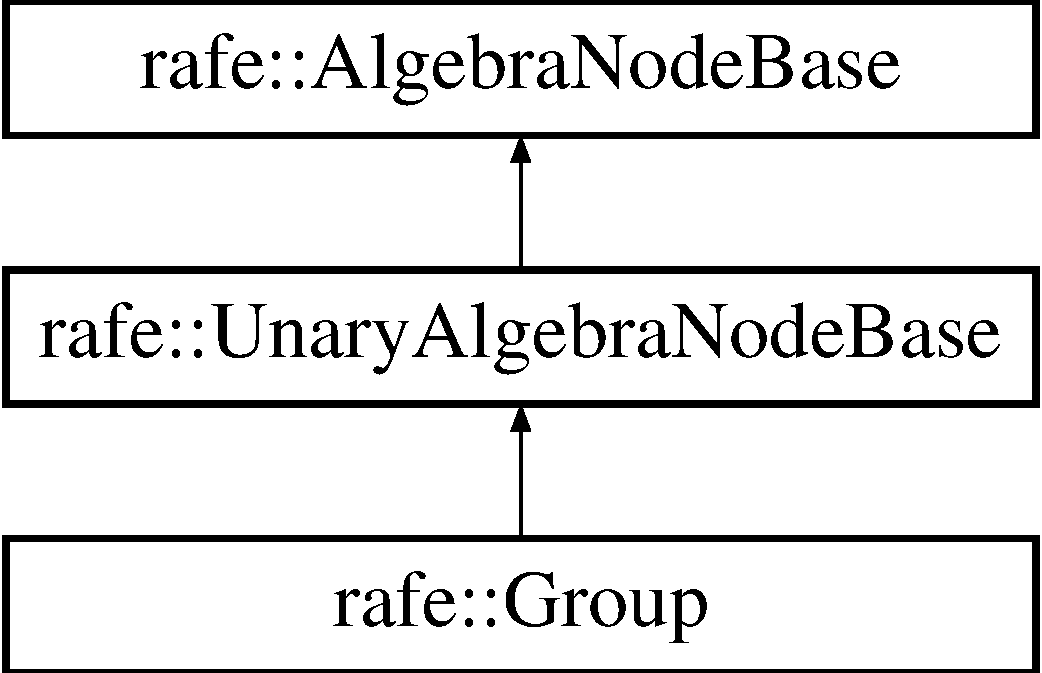
\includegraphics[height=3.000000cm]{classrafe_1_1_group}
\end{center}
\end{figure}
\subsection*{Public Member Functions}
\begin{DoxyCompactItemize}
\item 
\hyperlink{classrafe_1_1_group_a5536d2d9b3d8ce746697afc5eff32911}{Group} (D\+O\+M\+Element $\ast$element)
\item 
void \hyperlink{classrafe_1_1_group_ac2ef050b2a4c52f38cd7d5ab4bf52dfe}{accept} (\hyperlink{classrafe_1_1_algebra_visitor}{Algebra\+Visitor} \&v)
\end{DoxyCompactItemize}
\subsection*{Public Attributes}
\begin{DoxyCompactItemize}
\item 
std\+::vector$<$ \hyperlink{classrafe_1_1_group_column}{Group\+Column} $>$ \hyperlink{classrafe_1_1_group_a1b65b4d24bf834d05beb6ec00d9ed15b}{group\+Columns}
\item 
std\+::vector$<$ \hyperlink{classrafe_1_1_agregate_function}{Agregate\+Function} $>$ \hyperlink{classrafe_1_1_group_a774b152485b449b377745da5967a598d}{agregate\+Functions}
\end{DoxyCompactItemize}


\subsection{Detailed Description}
Represents the algebraic operation group. It groups by given columns and also computes agregate functions. 

\subsection{Constructor \& Destructor Documentation}
\hypertarget{classrafe_1_1_group_a5536d2d9b3d8ce746697afc5eff32911}{\index{rafe\+::\+Group@{rafe\+::\+Group}!Group@{Group}}
\index{Group@{Group}!rafe\+::\+Group@{rafe\+::\+Group}}
\subsubsection[{Group}]{\setlength{\rightskip}{0pt plus 5cm}rafe\+::\+Group\+::\+Group (
\begin{DoxyParamCaption}
\item[{D\+O\+M\+Element $\ast$}]{element}
\end{DoxyParamCaption}
)}}\label{classrafe_1_1_group_a5536d2d9b3d8ce746697afc5eff32911}
Creates the instance of \hyperlink{classrafe_1_1_group}{Group}. 
\begin{DoxyParams}{Parameters}
{\em element} & representing input node. \\
\hline
\end{DoxyParams}


\subsection{Member Function Documentation}
\hypertarget{classrafe_1_1_group_ac2ef050b2a4c52f38cd7d5ab4bf52dfe}{\index{rafe\+::\+Group@{rafe\+::\+Group}!accept@{accept}}
\index{accept@{accept}!rafe\+::\+Group@{rafe\+::\+Group}}
\subsubsection[{accept}]{\setlength{\rightskip}{0pt plus 5cm}void rafe\+::\+Group\+::accept (
\begin{DoxyParamCaption}
\item[{{\bf Algebra\+Visitor} \&}]{v}
\end{DoxyParamCaption}
)\hspace{0.3cm}{\ttfamily [virtual]}}}\label{classrafe_1_1_group_ac2ef050b2a4c52f38cd7d5ab4bf52dfe}
Method for calling visit\mbox{[}node\mbox{]} on given \hyperlink{classrafe_1_1_algebra_visitor}{Algebra\+Visitor}. 
\begin{DoxyParams}{Parameters}
{\em v} & \hyperlink{classrafe_1_1_algebra_visitor}{Algebra\+Visitor} which to call function on \\
\hline
\end{DoxyParams}


Implements \hyperlink{classrafe_1_1_unary_algebra_node_base_a6f554aad7250a0f15730d10ae24e4a79}{rafe\+::\+Unary\+Algebra\+Node\+Base}.



\subsection{Member Data Documentation}
\hypertarget{classrafe_1_1_group_a774b152485b449b377745da5967a598d}{\index{rafe\+::\+Group@{rafe\+::\+Group}!agregate\+Functions@{agregate\+Functions}}
\index{agregate\+Functions@{agregate\+Functions}!rafe\+::\+Group@{rafe\+::\+Group}}
\subsubsection[{agregate\+Functions}]{\setlength{\rightskip}{0pt plus 5cm}std\+::vector$<${\bf Agregate\+Function}$>$ rafe\+::\+Group\+::agregate\+Functions}}\label{classrafe_1_1_group_a774b152485b449b377745da5967a598d}
Stores aggregate function information associated with this group node. \hypertarget{classrafe_1_1_group_a1b65b4d24bf834d05beb6ec00d9ed15b}{\index{rafe\+::\+Group@{rafe\+::\+Group}!group\+Columns@{group\+Columns}}
\index{group\+Columns@{group\+Columns}!rafe\+::\+Group@{rafe\+::\+Group}}
\subsubsection[{group\+Columns}]{\setlength{\rightskip}{0pt plus 5cm}std\+::vector$<${\bf Group\+Column}$>$ rafe\+::\+Group\+::group\+Columns}}\label{classrafe_1_1_group_a1b65b4d24bf834d05beb6ec00d9ed15b}
Determines by which columns should current relation by grouped by. 

The documentation for this class was generated from the following files\+:\begin{DoxyCompactItemize}
\item 
C\+:/\+Users/\+Marcel/\+Documents/\+Visual Studio 2012/\+Projects/\+Relational\+Query\+Evaluator/\+Relational\+Query\+Evaluator/Algebra.\+h\item 
C\+:/\+Users/\+Marcel/\+Documents/\+Visual Studio 2012/\+Projects/\+Relational\+Query\+Evaluator/\+Relational\+Query\+Evaluator/Algebra.\+cpp\end{DoxyCompactItemize}

\hypertarget{classrafe_1_1_group_column}{\section{rafe\+:\+:Group\+Column Class Reference}
\label{classrafe_1_1_group_column}\index{rafe\+::\+Group\+Column@{rafe\+::\+Group\+Column}}
}


{\ttfamily \#include $<$Algebra\+Structures.\+h$>$}

\subsection*{Public Member Functions}
\begin{DoxyCompactItemize}
\item 
\hyperlink{classrafe_1_1_group_column_a003ad2331840ea07845a042ca9240970}{Group\+Column} (const \hyperlink{classrafe_1_1_column_identifier}{Column\+Identifier} \&\hyperlink{classrafe_1_1_group_column_a66b2532a7d69ddab17aae9c969927448}{input})
\end{DoxyCompactItemize}
\subsection*{Public Attributes}
\begin{DoxyCompactItemize}
\item 
\hyperlink{classrafe_1_1_column_identifier}{Column\+Identifier} \hyperlink{classrafe_1_1_group_column_a66b2532a7d69ddab17aae9c969927448}{input}
\item 
\hyperlink{classrafe_1_1_column_identifier}{Column\+Identifier} \hyperlink{classrafe_1_1_group_column_a830dc7de4321328cc1aba736ca0e82fe}{output}
\end{DoxyCompactItemize}


\subsection{Detailed Description}
Stores information about grouping column. 

\subsection{Constructor \& Destructor Documentation}
\hypertarget{classrafe_1_1_group_column_a003ad2331840ea07845a042ca9240970}{\index{rafe\+::\+Group\+Column@{rafe\+::\+Group\+Column}!Group\+Column@{Group\+Column}}
\index{Group\+Column@{Group\+Column}!rafe\+::\+Group\+Column@{rafe\+::\+Group\+Column}}
\subsubsection[{Group\+Column}]{\setlength{\rightskip}{0pt plus 5cm}rafe\+::\+Group\+Column\+::\+Group\+Column (
\begin{DoxyParamCaption}
\item[{const {\bf Column\+Identifier} \&}]{input}
\end{DoxyParamCaption}
)}}\label{classrafe_1_1_group_column_a003ad2331840ea07845a042ca9240970}
Create the instance of \hyperlink{classrafe_1_1_group_column}{Group\+Column} using \hyperlink{classrafe_1_1_column_identifier}{Column\+Identifier}. 
\begin{DoxyParams}{Parameters}
{\em input} & -\/ \hyperlink{classrafe_1_1_column_identifier}{Column\+Identifier} of the column \\
\hline
\end{DoxyParams}


\subsection{Member Data Documentation}
\hypertarget{classrafe_1_1_group_column_a66b2532a7d69ddab17aae9c969927448}{\index{rafe\+::\+Group\+Column@{rafe\+::\+Group\+Column}!input@{input}}
\index{input@{input}!rafe\+::\+Group\+Column@{rafe\+::\+Group\+Column}}
\subsubsection[{input}]{\setlength{\rightskip}{0pt plus 5cm}{\bf Column\+Identifier} rafe\+::\+Group\+Column\+::input}}\label{classrafe_1_1_group_column_a66b2532a7d69ddab17aae9c969927448}
Identifier of input column. \hypertarget{classrafe_1_1_group_column_a830dc7de4321328cc1aba736ca0e82fe}{\index{rafe\+::\+Group\+Column@{rafe\+::\+Group\+Column}!output@{output}}
\index{output@{output}!rafe\+::\+Group\+Column@{rafe\+::\+Group\+Column}}
\subsubsection[{output}]{\setlength{\rightskip}{0pt plus 5cm}{\bf Column\+Identifier} rafe\+::\+Group\+Column\+::output}}\label{classrafe_1_1_group_column_a830dc7de4321328cc1aba736ca0e82fe}
Identifier of output column. Input and output are same but they have different id. 

The documentation for this class was generated from the following files\+:\begin{DoxyCompactItemize}
\item 
C\+:/\+Users/\+Marcel/\+Documents/\+Visual Studio 2012/\+Projects/\+Relational\+Query\+Evaluator/\+Relational\+Query\+Evaluator/Algebra\+Structures.\+h\item 
C\+:/\+Users/\+Marcel/\+Documents/\+Visual Studio 2012/\+Projects/\+Relational\+Query\+Evaluator/\+Relational\+Query\+Evaluator/Algebra\+Structures.\+cpp\end{DoxyCompactItemize}

\hypertarget{classrafe_1_1_grouped_algebra_node}{\section{rafe\+:\+:Grouped\+Algebra\+Node Class Reference}
\label{classrafe_1_1_grouped_algebra_node}\index{rafe\+::\+Grouped\+Algebra\+Node@{rafe\+::\+Grouped\+Algebra\+Node}}
}


{\ttfamily \#include $<$Algebra.\+h$>$}

Inheritance diagram for rafe\+:\+:Grouped\+Algebra\+Node\+:\begin{figure}[H]
\begin{center}
\leavevmode
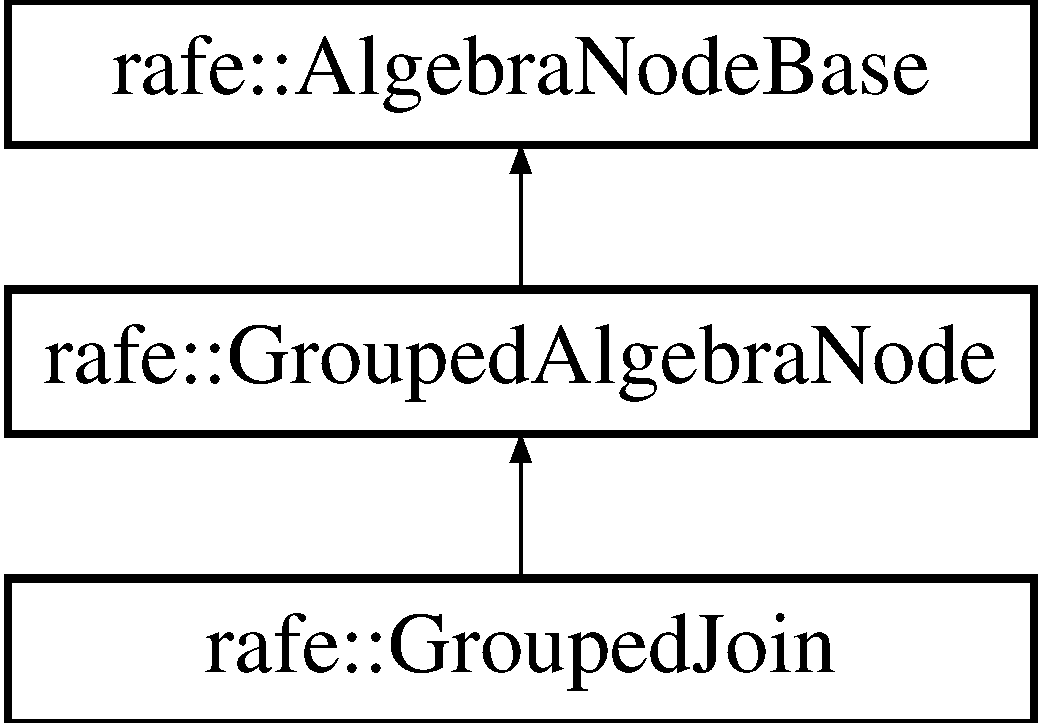
\includegraphics[height=3.000000cm]{classrafe_1_1_grouped_algebra_node}
\end{center}
\end{figure}
\subsection*{Public Member Functions}
\begin{DoxyCompactItemize}
\item 
virtual void \hyperlink{classrafe_1_1_grouped_algebra_node_abdb48442900d5560f815f4eb33ebeb04}{accept} (\hyperlink{classrafe_1_1_algebra_visitor}{Algebra\+Visitor} \&v)=0
\item 
std\+::shared\+\_\+ptr$<$ \hyperlink{classrafe_1_1_algebra_node_base}{Algebra\+Node\+Base} $>$ \hyperlink{classrafe_1_1_grouped_algebra_node_a3e19a9a32840f4deebec342963955634}{replace\+Child} (\hyperlink{classrafe_1_1_algebra_node_base}{Algebra\+Node\+Base} $\ast$old\+Child, std\+::shared\+\_\+ptr$<$ \hyperlink{classrafe_1_1_algebra_node_base}{Algebra\+Node\+Base} $>$ \&new\+Child)
\end{DoxyCompactItemize}
\subsection*{Public Attributes}
\begin{DoxyCompactItemize}
\item 
std\+::vector$<$ std\+::shared\+\_\+ptr\\*
$<$ \hyperlink{classrafe_1_1_algebra_node_base}{Algebra\+Node\+Base} $>$ $>$ \hyperlink{classrafe_1_1_grouped_algebra_node_ad7fdddb444ed50c118cece4fc1dd6783}{children}
\end{DoxyCompactItemize}


\subsection{Detailed Description}
Abstract class for n-\/nary algebraic operation. 

\subsection{Member Function Documentation}
\hypertarget{classrafe_1_1_grouped_algebra_node_abdb48442900d5560f815f4eb33ebeb04}{\index{rafe\+::\+Grouped\+Algebra\+Node@{rafe\+::\+Grouped\+Algebra\+Node}!accept@{accept}}
\index{accept@{accept}!rafe\+::\+Grouped\+Algebra\+Node@{rafe\+::\+Grouped\+Algebra\+Node}}
\subsubsection[{accept}]{\setlength{\rightskip}{0pt plus 5cm}virtual void rafe\+::\+Grouped\+Algebra\+Node\+::accept (
\begin{DoxyParamCaption}
\item[{{\bf Algebra\+Visitor} \&}]{v}
\end{DoxyParamCaption}
)\hspace{0.3cm}{\ttfamily [pure virtual]}}}\label{classrafe_1_1_grouped_algebra_node_abdb48442900d5560f815f4eb33ebeb04}
Method for calling visit\mbox{[}node\mbox{]} on given \hyperlink{classrafe_1_1_algebra_visitor}{Algebra\+Visitor}. 
\begin{DoxyParams}{Parameters}
{\em v} & \hyperlink{classrafe_1_1_algebra_visitor}{Algebra\+Visitor} which to call function on \\
\hline
\end{DoxyParams}


Implements \hyperlink{classrafe_1_1_algebra_node_base_a48e59b55cdb1c3d108343eb18920c1d1}{rafe\+::\+Algebra\+Node\+Base}.



Implemented in \hyperlink{classrafe_1_1_grouped_join_a36b56821dc719728f1f9294e3f8d8849}{rafe\+::\+Grouped\+Join}.

\hypertarget{classrafe_1_1_grouped_algebra_node_a3e19a9a32840f4deebec342963955634}{\index{rafe\+::\+Grouped\+Algebra\+Node@{rafe\+::\+Grouped\+Algebra\+Node}!replace\+Child@{replace\+Child}}
\index{replace\+Child@{replace\+Child}!rafe\+::\+Grouped\+Algebra\+Node@{rafe\+::\+Grouped\+Algebra\+Node}}
\subsubsection[{replace\+Child}]{\setlength{\rightskip}{0pt plus 5cm}shared\+\_\+ptr$<$ {\bf Algebra\+Node\+Base} $>$ rafe\+::\+Grouped\+Algebra\+Node\+::replace\+Child (
\begin{DoxyParamCaption}
\item[{{\bf Algebra\+Node\+Base} $\ast$}]{old\+Child, }
\item[{std\+::shared\+\_\+ptr$<$ {\bf Algebra\+Node\+Base} $>$ \&}]{new\+Child}
\end{DoxyParamCaption}
)\hspace{0.3cm}{\ttfamily [virtual]}}}\label{classrafe_1_1_grouped_algebra_node_a3e19a9a32840f4deebec342963955634}
Replaces one child of this node with other one 
\begin{DoxyParams}{Parameters}
{\em old\+Child} & node to be replaced \\
\hline
{\em new\+Child} & new node to replace the old one \\
\hline
\end{DoxyParams}
\begin{DoxyReturn}{Returns}
replaced child 
\end{DoxyReturn}


Implements \hyperlink{classrafe_1_1_algebra_node_base_ac6d722e739dd39c223bb129dfbd0ab45}{rafe\+::\+Algebra\+Node\+Base}.



\subsection{Member Data Documentation}
\hypertarget{classrafe_1_1_grouped_algebra_node_ad7fdddb444ed50c118cece4fc1dd6783}{\index{rafe\+::\+Grouped\+Algebra\+Node@{rafe\+::\+Grouped\+Algebra\+Node}!children@{children}}
\index{children@{children}!rafe\+::\+Grouped\+Algebra\+Node@{rafe\+::\+Grouped\+Algebra\+Node}}
\subsubsection[{children}]{\setlength{\rightskip}{0pt plus 5cm}std\+::vector$<$std\+::shared\+\_\+ptr$<${\bf Algebra\+Node\+Base}$>$ $>$ rafe\+::\+Grouped\+Algebra\+Node\+::children}}\label{classrafe_1_1_grouped_algebra_node_ad7fdddb444ed50c118cece4fc1dd6783}
Stores list containg children of this node. 

The documentation for this class was generated from the following files\+:\begin{DoxyCompactItemize}
\item 
C\+:/\+Users/\+Marcel/\+Documents/\+Visual Studio 2012/\+Projects/\+Relational\+Query\+Evaluator/\+Relational\+Query\+Evaluator/Algebra.\+h\item 
C\+:/\+Users/\+Marcel/\+Documents/\+Visual Studio 2012/\+Projects/\+Relational\+Query\+Evaluator/\+Relational\+Query\+Evaluator/Algebra.\+cpp\end{DoxyCompactItemize}

\hypertarget{classrafe_1_1_grouped_expression}{\section{rafe\+:\+:Grouped\+Expression Class Reference}
\label{classrafe_1_1_grouped_expression}\index{rafe\+::\+Grouped\+Expression@{rafe\+::\+Grouped\+Expression}}
}


{\ttfamily \#include $<$Expressions.\+h$>$}

Inheritance diagram for rafe\+:\+:Grouped\+Expression\+:\begin{figure}[H]
\begin{center}
\leavevmode
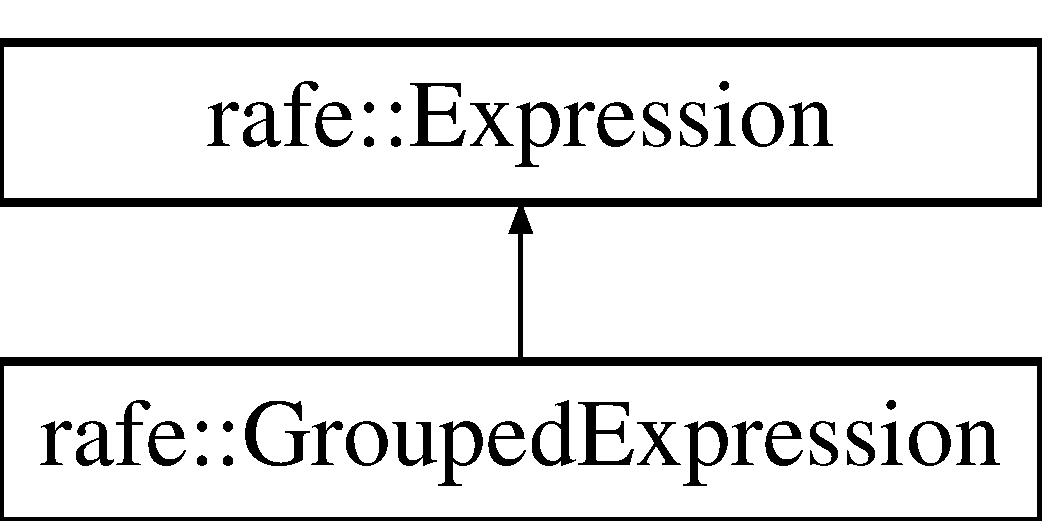
\includegraphics[height=2.000000cm]{classrafe_1_1_grouped_expression}
\end{center}
\end{figure}
\subsection*{Public Member Functions}
\begin{DoxyCompactItemize}
\item 
\hyperlink{classrafe_1_1_grouped_expression_a0f8325955c030168ab4590f631bcb0cf}{Grouped\+Expression} ()
\item 
\hyperlink{classrafe_1_1_grouped_expression_ab057facf61cab70b5a8e7aeb5438a55d}{Grouped\+Expression} (Grouped\+Operator \hyperlink{classrafe_1_1_grouped_expression_a269644ee2565184c9386dd57d24e93bb}{operation}, const std\+::vector$<$ std\+::shared\+\_\+ptr$<$ \hyperlink{classrafe_1_1_expression}{Expression} $>$$>$ \&\hyperlink{classrafe_1_1_grouped_expression_af31df501bd0d3e5ee9ce28ab4c71c4ee}{children})
\item 
void \hyperlink{classrafe_1_1_grouped_expression_a7f7e2cb9efd9457d80dc6365339957f6}{accept} (\hyperlink{classrafe_1_1_expression_visitor_base}{Expression\+Visitor\+Base} \&v)
\item 
void \hyperlink{classrafe_1_1_grouped_expression_ab770657757c0b374e4eacc8112ba9c4f}{replace\+Child} (\hyperlink{classrafe_1_1_expression}{Expression} $\ast$old\+Child, std\+::shared\+\_\+ptr$<$ \hyperlink{classrafe_1_1_expression}{Expression} $>$ new\+Child)
\end{DoxyCompactItemize}
\subsection*{Public Attributes}
\begin{DoxyCompactItemize}
\item 
Grouped\+Operator \hyperlink{classrafe_1_1_grouped_expression_a269644ee2565184c9386dd57d24e93bb}{operation}
\item 
std\+::vector$<$ std\+::shared\+\_\+ptr\\*
$<$ \hyperlink{classrafe_1_1_expression}{Expression} $>$ $>$ \hyperlink{classrafe_1_1_grouped_expression_af31df501bd0d3e5ee9ce28ab4c71c4ee}{children}
\end{DoxyCompactItemize}
\subsection*{Additional Inherited Members}


\subsection{Detailed Description}
Represents grouped logical or aritmetic comutative expression. It has variable number of children. It is currently used for A\+N\+D and O\+R operations. 

\subsection{Constructor \& Destructor Documentation}
\hypertarget{classrafe_1_1_grouped_expression_a0f8325955c030168ab4590f631bcb0cf}{\index{rafe\+::\+Grouped\+Expression@{rafe\+::\+Grouped\+Expression}!Grouped\+Expression@{Grouped\+Expression}}
\index{Grouped\+Expression@{Grouped\+Expression}!rafe\+::\+Grouped\+Expression@{rafe\+::\+Grouped\+Expression}}
\subsubsection[{Grouped\+Expression}]{\setlength{\rightskip}{0pt plus 5cm}rafe\+::\+Grouped\+Expression\+::\+Grouped\+Expression (
\begin{DoxyParamCaption}
{}
\end{DoxyParamCaption}
)}}\label{classrafe_1_1_grouped_expression_a0f8325955c030168ab4590f631bcb0cf}
Creates new instance of Groupped\+Expression. \hypertarget{classrafe_1_1_grouped_expression_ab057facf61cab70b5a8e7aeb5438a55d}{\index{rafe\+::\+Grouped\+Expression@{rafe\+::\+Grouped\+Expression}!Grouped\+Expression@{Grouped\+Expression}}
\index{Grouped\+Expression@{Grouped\+Expression}!rafe\+::\+Grouped\+Expression@{rafe\+::\+Grouped\+Expression}}
\subsubsection[{Grouped\+Expression}]{\setlength{\rightskip}{0pt plus 5cm}rafe\+::\+Grouped\+Expression\+::\+Grouped\+Expression (
\begin{DoxyParamCaption}
\item[{Grouped\+Operator}]{operation, }
\item[{const std\+::vector$<$ std\+::shared\+\_\+ptr$<$ {\bf Expression} $>$$>$ \&}]{children}
\end{DoxyParamCaption}
)}}\label{classrafe_1_1_grouped_expression_ab057facf61cab70b5a8e7aeb5438a55d}
Creates new instance of Groupped\+Expression. 
\begin{DoxyParams}{Parameters}
{\em operation} & -\/ type of operation. \\
\hline
{\em children} & -\/ child nodes. \\
\hline
\end{DoxyParams}


\subsection{Member Function Documentation}
\hypertarget{classrafe_1_1_grouped_expression_a7f7e2cb9efd9457d80dc6365339957f6}{\index{rafe\+::\+Grouped\+Expression@{rafe\+::\+Grouped\+Expression}!accept@{accept}}
\index{accept@{accept}!rafe\+::\+Grouped\+Expression@{rafe\+::\+Grouped\+Expression}}
\subsubsection[{accept}]{\setlength{\rightskip}{0pt plus 5cm}void rafe\+::\+Grouped\+Expression\+::accept (
\begin{DoxyParamCaption}
\item[{{\bf Expression\+Visitor\+Base} \&}]{v}
\end{DoxyParamCaption}
)\hspace{0.3cm}{\ttfamily [virtual]}}}\label{classrafe_1_1_grouped_expression_a7f7e2cb9efd9457d80dc6365339957f6}
Method for calling visit\mbox{[}node\mbox{]} on given Expression\+Visitor. 
\begin{DoxyParams}{Parameters}
{\em v} & Expression\+Visitor, on which to call visit function. \\
\hline
\end{DoxyParams}


Implements \hyperlink{classrafe_1_1_expression_a3b2e5bae8b99ea6c9a3c92a9b949b3cd}{rafe\+::\+Expression}.

\hypertarget{classrafe_1_1_grouped_expression_ab770657757c0b374e4eacc8112ba9c4f}{\index{rafe\+::\+Grouped\+Expression@{rafe\+::\+Grouped\+Expression}!replace\+Child@{replace\+Child}}
\index{replace\+Child@{replace\+Child}!rafe\+::\+Grouped\+Expression@{rafe\+::\+Grouped\+Expression}}
\subsubsection[{replace\+Child}]{\setlength{\rightskip}{0pt plus 5cm}void rafe\+::\+Grouped\+Expression\+::replace\+Child (
\begin{DoxyParamCaption}
\item[{{\bf Expression} $\ast$}]{old\+Child, }
\item[{std\+::shared\+\_\+ptr$<$ {\bf Expression} $>$}]{new\+Child}
\end{DoxyParamCaption}
)\hspace{0.3cm}{\ttfamily [virtual]}}}\label{classrafe_1_1_grouped_expression_ab770657757c0b374e4eacc8112ba9c4f}
Replaces child from this class with new expression tree. 
\begin{DoxyParams}{Parameters}
{\em old\+Child} & -\/ child to replace. \\
\hline
{\em new\+Child} & -\/ child to be replaced. \\
\hline
\end{DoxyParams}


Implements \hyperlink{classrafe_1_1_expression_a841879e8eb85f4bb68cfeec24231a701}{rafe\+::\+Expression}.



\subsection{Member Data Documentation}
\hypertarget{classrafe_1_1_grouped_expression_af31df501bd0d3e5ee9ce28ab4c71c4ee}{\index{rafe\+::\+Grouped\+Expression@{rafe\+::\+Grouped\+Expression}!children@{children}}
\index{children@{children}!rafe\+::\+Grouped\+Expression@{rafe\+::\+Grouped\+Expression}}
\subsubsection[{children}]{\setlength{\rightskip}{0pt plus 5cm}std\+::vector$<$std\+::shared\+\_\+ptr$<${\bf Expression}$>$ $>$ rafe\+::\+Grouped\+Expression\+::children}}\label{classrafe_1_1_grouped_expression_af31df501bd0d3e5ee9ce28ab4c71c4ee}
Stores call arguments. Arguments are also expression trees. \hypertarget{classrafe_1_1_grouped_expression_a269644ee2565184c9386dd57d24e93bb}{\index{rafe\+::\+Grouped\+Expression@{rafe\+::\+Grouped\+Expression}!operation@{operation}}
\index{operation@{operation}!rafe\+::\+Grouped\+Expression@{rafe\+::\+Grouped\+Expression}}
\subsubsection[{operation}]{\setlength{\rightskip}{0pt plus 5cm}Grouped\+Operator rafe\+::\+Grouped\+Expression\+::operation}}\label{classrafe_1_1_grouped_expression_a269644ee2565184c9386dd57d24e93bb}
Identifies column with name and unique id. 

The documentation for this class was generated from the following files\+:\begin{DoxyCompactItemize}
\item 
C\+:/\+Users/\+Marcel/\+Documents/\+Visual Studio 2012/\+Projects/\+Relational\+Query\+Evaluator/\+Relational\+Query\+Evaluator/Expressions.\+h\item 
C\+:/\+Users/\+Marcel/\+Documents/\+Visual Studio 2012/\+Projects/\+Relational\+Query\+Evaluator/\+Relational\+Query\+Evaluator/Expressions.\+cpp\end{DoxyCompactItemize}

\hypertarget{classrafe_1_1_grouped_join}{\section{rafe\+:\+:Grouped\+Join Class Reference}
\label{classrafe_1_1_grouped_join}\index{rafe\+::\+Grouped\+Join@{rafe\+::\+Grouped\+Join}}
}


{\ttfamily \#include $<$Algebra.\+h$>$}

Inheritance diagram for rafe\+:\+:Grouped\+Join\+:\begin{figure}[H]
\begin{center}
\leavevmode
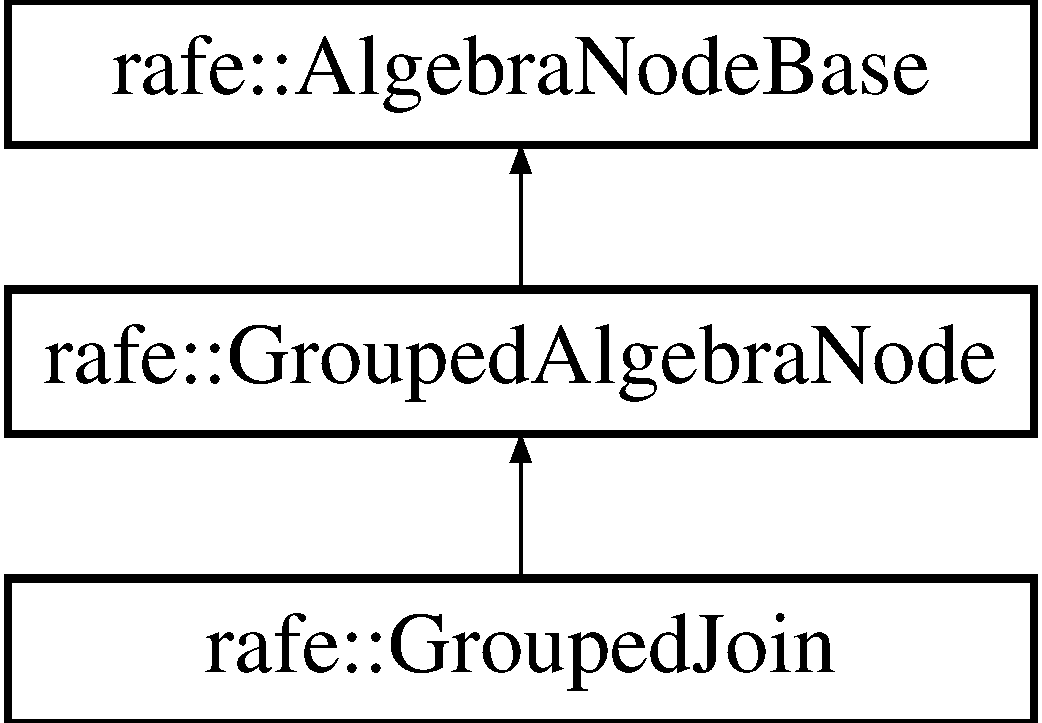
\includegraphics[height=3.000000cm]{classrafe_1_1_grouped_join}
\end{center}
\end{figure}
\subsection*{Public Member Functions}
\begin{DoxyCompactItemize}
\item 
void \hyperlink{classrafe_1_1_grouped_join_a36b56821dc719728f1f9294e3f8d8849}{accept} (\hyperlink{classrafe_1_1_algebra_visitor}{Algebra\+Visitor} \&v)
\end{DoxyCompactItemize}
\subsection*{Public Attributes}
\begin{DoxyCompactItemize}
\item 
std\+::shared\+\_\+ptr$<$ \hyperlink{classrafe_1_1_expression}{Expression} $>$ \hyperlink{classrafe_1_1_grouped_join_a9217fbe67d211897dca2d54d0825e86b}{condition}
\item 
std\+::vector$<$ \hyperlink{classrafe_1_1_join_column_info}{Join\+Column\+Info} $>$ \hyperlink{classrafe_1_1_grouped_join_aae2b6f6d25f2b8467dacac459e0a8abb}{output\+Join\+Columns}
\end{DoxyCompactItemize}


\subsection{Detailed Description}
Represents the algebraic operation join on multiple tables. 

\subsection{Member Function Documentation}
\hypertarget{classrafe_1_1_grouped_join_a36b56821dc719728f1f9294e3f8d8849}{\index{rafe\+::\+Grouped\+Join@{rafe\+::\+Grouped\+Join}!accept@{accept}}
\index{accept@{accept}!rafe\+::\+Grouped\+Join@{rafe\+::\+Grouped\+Join}}
\subsubsection[{accept}]{\setlength{\rightskip}{0pt plus 5cm}void rafe\+::\+Grouped\+Join\+::accept (
\begin{DoxyParamCaption}
\item[{{\bf Algebra\+Visitor} \&}]{v}
\end{DoxyParamCaption}
)\hspace{0.3cm}{\ttfamily [virtual]}}}\label{classrafe_1_1_grouped_join_a36b56821dc719728f1f9294e3f8d8849}
Method for calling visit\mbox{[}node\mbox{]} on given \hyperlink{classrafe_1_1_algebra_visitor}{Algebra\+Visitor}. 
\begin{DoxyParams}{Parameters}
{\em v} & \hyperlink{classrafe_1_1_algebra_visitor}{Algebra\+Visitor} on which to call function. \\
\hline
\end{DoxyParams}


Implements \hyperlink{classrafe_1_1_grouped_algebra_node_abdb48442900d5560f815f4eb33ebeb04}{rafe\+::\+Grouped\+Algebra\+Node}.



\subsection{Member Data Documentation}
\hypertarget{classrafe_1_1_grouped_join_a9217fbe67d211897dca2d54d0825e86b}{\index{rafe\+::\+Grouped\+Join@{rafe\+::\+Grouped\+Join}!condition@{condition}}
\index{condition@{condition}!rafe\+::\+Grouped\+Join@{rafe\+::\+Grouped\+Join}}
\subsubsection[{condition}]{\setlength{\rightskip}{0pt plus 5cm}std\+::shared\+\_\+ptr$<${\bf Expression}$>$ rafe\+::\+Grouped\+Join\+::condition}}\label{classrafe_1_1_grouped_join_a9217fbe67d211897dca2d54d0825e86b}
Condition for joining. \hypertarget{classrafe_1_1_grouped_join_aae2b6f6d25f2b8467dacac459e0a8abb}{\index{rafe\+::\+Grouped\+Join@{rafe\+::\+Grouped\+Join}!output\+Join\+Columns@{output\+Join\+Columns}}
\index{output\+Join\+Columns@{output\+Join\+Columns}!rafe\+::\+Grouped\+Join@{rafe\+::\+Grouped\+Join}}
\subsubsection[{output\+Join\+Columns}]{\setlength{\rightskip}{0pt plus 5cm}std\+::vector$<${\bf Join\+Column\+Info}$>$ rafe\+::\+Grouped\+Join\+::output\+Join\+Columns}}\label{classrafe_1_1_grouped_join_aae2b6f6d25f2b8467dacac459e0a8abb}
List of output columns from join operator. 

The documentation for this class was generated from the following files\+:\begin{DoxyCompactItemize}
\item 
C\+:/\+Users/\+Marcel/\+Documents/\+Visual Studio 2012/\+Projects/\+Relational\+Query\+Evaluator/\+Relational\+Query\+Evaluator/Algebra.\+h\item 
C\+:/\+Users/\+Marcel/\+Documents/\+Visual Studio 2012/\+Projects/\+Relational\+Query\+Evaluator/\+Relational\+Query\+Evaluator/Algebra.\+cpp\end{DoxyCompactItemize}

\hypertarget{classrafe_1_1_grouping_expression_visitor}{\section{rafe\+:\+:Grouping\+Expression\+Visitor Class Reference}
\label{classrafe_1_1_grouping_expression_visitor}\index{rafe\+::\+Grouping\+Expression\+Visitor@{rafe\+::\+Grouping\+Expression\+Visitor}}
}


{\ttfamily \#include $<$Expression\+Visitors.\+h$>$}

Inheritance diagram for rafe\+:\+:Grouping\+Expression\+Visitor\+:\begin{figure}[H]
\begin{center}
\leavevmode
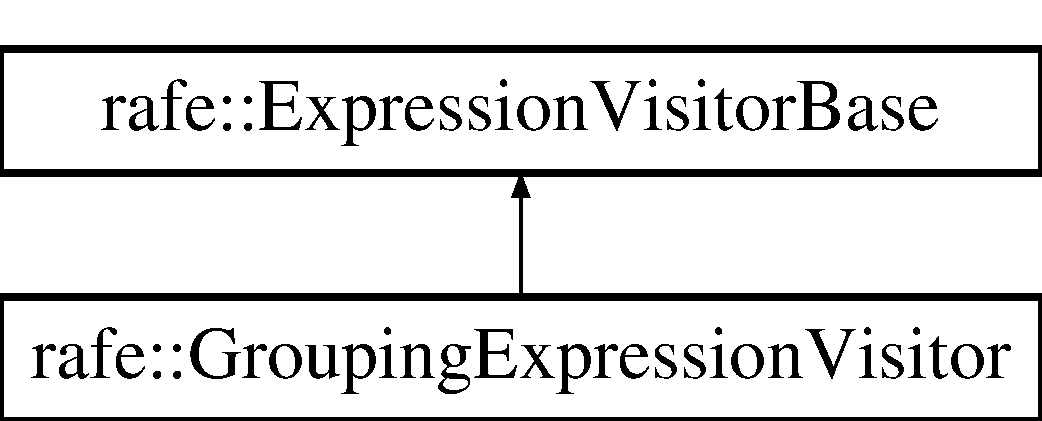
\includegraphics[height=2.000000cm]{classrafe_1_1_grouping_expression_visitor}
\end{center}
\end{figure}
\subsection*{Public Member Functions}
\begin{DoxyCompactItemize}
\item 
\hyperlink{classrafe_1_1_grouping_expression_visitor_ae171337286854c9bd3c3c5eb73c465c7}{Grouping\+Expression\+Visitor} (std\+::shared\+\_\+ptr$<$ \hyperlink{classrafe_1_1_expression}{Expression} $>$ $\ast$x)
\item 
void \hyperlink{classrafe_1_1_grouping_expression_visitor_a5ef6febb7f733f4adcf61bc83a6d10f8}{visit\+Binary\+Expression} (\hyperlink{classrafe_1_1_binary_expression}{Binary\+Expression} $\ast$expression)
\end{DoxyCompactItemize}
\subsection*{Public Attributes}
\begin{DoxyCompactItemize}
\item 
std\+::shared\+\_\+ptr$<$ \hyperlink{classrafe_1_1_expression}{Expression} $>$ $\ast$ \hyperlink{classrafe_1_1_grouping_expression_visitor_a95a43ca2fdb2670f5407d7b38fff1e9e}{root}
\end{DoxyCompactItemize}


\subsection{Detailed Description}
This visitor merges all neighbouring A\+N\+D and O\+R binary expression into Grouped expression. 

\subsection{Constructor \& Destructor Documentation}
\hypertarget{classrafe_1_1_grouping_expression_visitor_ae171337286854c9bd3c3c5eb73c465c7}{\index{rafe\+::\+Grouping\+Expression\+Visitor@{rafe\+::\+Grouping\+Expression\+Visitor}!Grouping\+Expression\+Visitor@{Grouping\+Expression\+Visitor}}
\index{Grouping\+Expression\+Visitor@{Grouping\+Expression\+Visitor}!rafe\+::\+Grouping\+Expression\+Visitor@{rafe\+::\+Grouping\+Expression\+Visitor}}
\subsubsection[{Grouping\+Expression\+Visitor}]{\setlength{\rightskip}{0pt plus 5cm}rafe\+::\+Grouping\+Expression\+Visitor\+::\+Grouping\+Expression\+Visitor (
\begin{DoxyParamCaption}
\item[{std\+::shared\+\_\+ptr$<$ {\bf Expression} $>$ $\ast$}]{x}
\end{DoxyParamCaption}
)}}\label{classrafe_1_1_grouping_expression_visitor_ae171337286854c9bd3c3c5eb73c465c7}
Creates new instance of \hyperlink{classrafe_1_1_grouping_expression_visitor}{Grouping\+Expression\+Visitor}. 
\begin{DoxyParams}{Parameters}
{\em x} & -\/ root of visited expression tree. \\
\hline
\end{DoxyParams}


\subsection{Member Function Documentation}
\hypertarget{classrafe_1_1_grouping_expression_visitor_a5ef6febb7f733f4adcf61bc83a6d10f8}{\index{rafe\+::\+Grouping\+Expression\+Visitor@{rafe\+::\+Grouping\+Expression\+Visitor}!visit\+Binary\+Expression@{visit\+Binary\+Expression}}
\index{visit\+Binary\+Expression@{visit\+Binary\+Expression}!rafe\+::\+Grouping\+Expression\+Visitor@{rafe\+::\+Grouping\+Expression\+Visitor}}
\subsubsection[{visit\+Binary\+Expression}]{\setlength{\rightskip}{0pt plus 5cm}void rafe\+::\+Grouping\+Expression\+Visitor\+::visit\+Binary\+Expression (
\begin{DoxyParamCaption}
\item[{{\bf Binary\+Expression} $\ast$}]{expression}
\end{DoxyParamCaption}
)\hspace{0.3cm}{\ttfamily [virtual]}}}\label{classrafe_1_1_grouping_expression_visitor_a5ef6febb7f733f4adcf61bc83a6d10f8}
Visits \hyperlink{classrafe_1_1_binary_expression}{Binary\+Expression} element. 
\begin{DoxyParams}{Parameters}
{\em expression} & visited \hyperlink{classrafe_1_1_binary_expression}{Binary\+Expression}. \\
\hline
\end{DoxyParams}


Reimplemented from \hyperlink{classrafe_1_1_expression_visitor_base_a63e53276af3a22d3592f34d05ba97014}{rafe\+::\+Expression\+Visitor\+Base}.



\subsection{Member Data Documentation}
\hypertarget{classrafe_1_1_grouping_expression_visitor_a95a43ca2fdb2670f5407d7b38fff1e9e}{\index{rafe\+::\+Grouping\+Expression\+Visitor@{rafe\+::\+Grouping\+Expression\+Visitor}!root@{root}}
\index{root@{root}!rafe\+::\+Grouping\+Expression\+Visitor@{rafe\+::\+Grouping\+Expression\+Visitor}}
\subsubsection[{root}]{\setlength{\rightskip}{0pt plus 5cm}std\+::shared\+\_\+ptr$<${\bf Expression}$>$$\ast$ rafe\+::\+Grouping\+Expression\+Visitor\+::root}}\label{classrafe_1_1_grouping_expression_visitor_a95a43ca2fdb2670f5407d7b38fff1e9e}
Root of expression tree. If the root is changed it root has to be rewritten. 

The documentation for this class was generated from the following files\+:\begin{DoxyCompactItemize}
\item 
C\+:/\+Users/\+Marcel/\+Documents/\+Visual Studio 2012/\+Projects/\+Relational\+Query\+Evaluator/\+Relational\+Query\+Evaluator/Expression\+Visitors.\+h\item 
C\+:/\+Users/\+Marcel/\+Documents/\+Visual Studio 2012/\+Projects/\+Relational\+Query\+Evaluator/\+Relational\+Query\+Evaluator/Expression\+Visitors.\+cpp\end{DoxyCompactItemize}

\hypertarget{classrafe_1_1_grouping_visitor}{\section{rafe\+:\+:Grouping\+Visitor Class Reference}
\label{classrafe_1_1_grouping_visitor}\index{rafe\+::\+Grouping\+Visitor@{rafe\+::\+Grouping\+Visitor}}
}


{\ttfamily \#include $<$Algebra\+Visitors.\+h$>$}

Inheritance diagram for rafe\+:\+:Grouping\+Visitor\+:\begin{figure}[H]
\begin{center}
\leavevmode
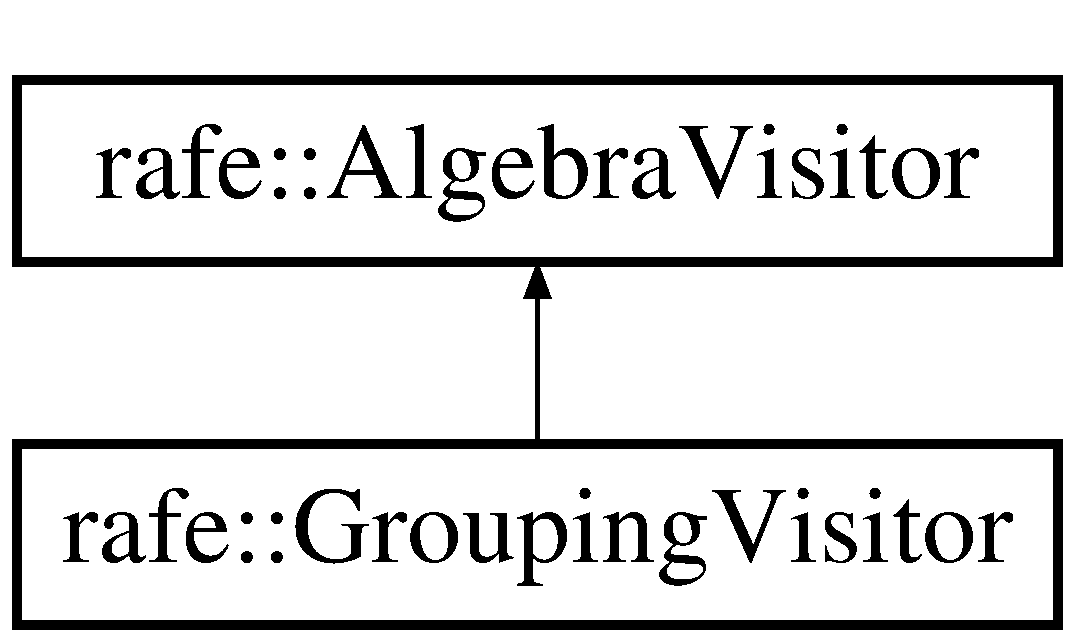
\includegraphics[height=2.000000cm]{classrafe_1_1_grouping_visitor}
\end{center}
\end{figure}
\subsection*{Public Member Functions}
\begin{DoxyCompactItemize}
\item 
\hyperlink{classrafe_1_1_grouping_visitor_a33accac3eae9e1ecb557acf7c7867d45}{Grouping\+Visitor} ()
\item 
void \hyperlink{classrafe_1_1_grouping_visitor_acb0f1d2cd1d7432d812191841efc6f60}{visit\+Column\+Operations} (\hyperlink{classrafe_1_1_column_operations}{Column\+Operations} $\ast$node)
\item 
void \hyperlink{classrafe_1_1_grouping_visitor_a7287bb0601e55028ef362604144eae23}{visit\+Selection} (\hyperlink{classrafe_1_1_selection}{Selection} $\ast$node)
\item 
void \hyperlink{classrafe_1_1_grouping_visitor_a519732d6b549b84cd543ab61aa7630f1}{visit\+Join} (\hyperlink{classrafe_1_1_join}{Join} $\ast$node)
\item 
void \hyperlink{classrafe_1_1_grouping_visitor_aa5f7889f7fc5ec289d7ee1107b441c0c}{visit\+Anti\+Join} (\hyperlink{classrafe_1_1_anti_join}{Anti\+Join} $\ast$node)
\end{DoxyCompactItemize}
\subsection*{Additional Inherited Members}


\subsection{Detailed Description}
This algebra visitor groupes neighbour join into one groupped join. It also calls \hyperlink{classrafe_1_1_grouping_expression_visitor}{Grouping\+Expression\+Visitor} on every condition. 

\subsection{Constructor \& Destructor Documentation}
\hypertarget{classrafe_1_1_grouping_visitor_a33accac3eae9e1ecb557acf7c7867d45}{\index{rafe\+::\+Grouping\+Visitor@{rafe\+::\+Grouping\+Visitor}!Grouping\+Visitor@{Grouping\+Visitor}}
\index{Grouping\+Visitor@{Grouping\+Visitor}!rafe\+::\+Grouping\+Visitor@{rafe\+::\+Grouping\+Visitor}}
\subsubsection[{Grouping\+Visitor}]{\setlength{\rightskip}{0pt plus 5cm}rafe\+::\+Grouping\+Visitor\+::\+Grouping\+Visitor (
\begin{DoxyParamCaption}
{}
\end{DoxyParamCaption}
)}}\label{classrafe_1_1_grouping_visitor_a33accac3eae9e1ecb557acf7c7867d45}
Creates new instance of \hyperlink{classrafe_1_1_grouping_visitor}{Grouping\+Visitor}. 

\subsection{Member Function Documentation}
\hypertarget{classrafe_1_1_grouping_visitor_aa5f7889f7fc5ec289d7ee1107b441c0c}{\index{rafe\+::\+Grouping\+Visitor@{rafe\+::\+Grouping\+Visitor}!visit\+Anti\+Join@{visit\+Anti\+Join}}
\index{visit\+Anti\+Join@{visit\+Anti\+Join}!rafe\+::\+Grouping\+Visitor@{rafe\+::\+Grouping\+Visitor}}
\subsubsection[{visit\+Anti\+Join}]{\setlength{\rightskip}{0pt plus 5cm}void rafe\+::\+Grouping\+Visitor\+::visit\+Anti\+Join (
\begin{DoxyParamCaption}
\item[{{\bf Anti\+Join} $\ast$}]{node}
\end{DoxyParamCaption}
)\hspace{0.3cm}{\ttfamily [virtual]}}}\label{classrafe_1_1_grouping_visitor_aa5f7889f7fc5ec289d7ee1107b441c0c}
Visits \hyperlink{classrafe_1_1_anti_join}{Anti\+Join} element. 
\begin{DoxyParams}{Parameters}
{\em node} & visited \hyperlink{classrafe_1_1_anti_join}{Anti\+Join}. \\
\hline
\end{DoxyParams}


Reimplemented from \hyperlink{classrafe_1_1_algebra_visitor_a8b31789473135aff92e900a6a7765eda}{rafe\+::\+Algebra\+Visitor}.

\hypertarget{classrafe_1_1_grouping_visitor_acb0f1d2cd1d7432d812191841efc6f60}{\index{rafe\+::\+Grouping\+Visitor@{rafe\+::\+Grouping\+Visitor}!visit\+Column\+Operations@{visit\+Column\+Operations}}
\index{visit\+Column\+Operations@{visit\+Column\+Operations}!rafe\+::\+Grouping\+Visitor@{rafe\+::\+Grouping\+Visitor}}
\subsubsection[{visit\+Column\+Operations}]{\setlength{\rightskip}{0pt plus 5cm}void rafe\+::\+Grouping\+Visitor\+::visit\+Column\+Operations (
\begin{DoxyParamCaption}
\item[{{\bf Column\+Operations} $\ast$}]{node}
\end{DoxyParamCaption}
)\hspace{0.3cm}{\ttfamily [virtual]}}}\label{classrafe_1_1_grouping_visitor_acb0f1d2cd1d7432d812191841efc6f60}
Visits \hyperlink{classrafe_1_1_column_operations}{Column\+Operations} element. 
\begin{DoxyParams}{Parameters}
{\em node} & visited \hyperlink{classrafe_1_1_column_operations}{Column\+Operations}. \\
\hline
\end{DoxyParams}


Reimplemented from \hyperlink{classrafe_1_1_algebra_visitor_a518ce4d12f874a6c2f1fb0bb961144f8}{rafe\+::\+Algebra\+Visitor}.

\hypertarget{classrafe_1_1_grouping_visitor_a519732d6b549b84cd543ab61aa7630f1}{\index{rafe\+::\+Grouping\+Visitor@{rafe\+::\+Grouping\+Visitor}!visit\+Join@{visit\+Join}}
\index{visit\+Join@{visit\+Join}!rafe\+::\+Grouping\+Visitor@{rafe\+::\+Grouping\+Visitor}}
\subsubsection[{visit\+Join}]{\setlength{\rightskip}{0pt plus 5cm}void rafe\+::\+Grouping\+Visitor\+::visit\+Join (
\begin{DoxyParamCaption}
\item[{{\bf Join} $\ast$}]{node}
\end{DoxyParamCaption}
)\hspace{0.3cm}{\ttfamily [virtual]}}}\label{classrafe_1_1_grouping_visitor_a519732d6b549b84cd543ab61aa7630f1}
Visits \hyperlink{classrafe_1_1_join}{Join} element. 
\begin{DoxyParams}{Parameters}
{\em node} & visited \hyperlink{classrafe_1_1_join}{Join}. \\
\hline
\end{DoxyParams}


Reimplemented from \hyperlink{classrafe_1_1_algebra_visitor_ab499694bc7ccd718c6f7a5c4f3d33f1c}{rafe\+::\+Algebra\+Visitor}.

\hypertarget{classrafe_1_1_grouping_visitor_a7287bb0601e55028ef362604144eae23}{\index{rafe\+::\+Grouping\+Visitor@{rafe\+::\+Grouping\+Visitor}!visit\+Selection@{visit\+Selection}}
\index{visit\+Selection@{visit\+Selection}!rafe\+::\+Grouping\+Visitor@{rafe\+::\+Grouping\+Visitor}}
\subsubsection[{visit\+Selection}]{\setlength{\rightskip}{0pt plus 5cm}void rafe\+::\+Grouping\+Visitor\+::visit\+Selection (
\begin{DoxyParamCaption}
\item[{{\bf Selection} $\ast$}]{node}
\end{DoxyParamCaption}
)\hspace{0.3cm}{\ttfamily [virtual]}}}\label{classrafe_1_1_grouping_visitor_a7287bb0601e55028ef362604144eae23}
Visits \hyperlink{classrafe_1_1_selection}{Selection} element. 
\begin{DoxyParams}{Parameters}
{\em node} & visited \hyperlink{classrafe_1_1_selection}{Selection}. \\
\hline
\end{DoxyParams}


Reimplemented from \hyperlink{classrafe_1_1_algebra_visitor_a81f691749cb29da00bee299c617b9044}{rafe\+::\+Algebra\+Visitor}.



The documentation for this class was generated from the following files\+:\begin{DoxyCompactItemize}
\item 
C\+:/\+Users/\+Marcel/\+Documents/\+Visual Studio 2012/\+Projects/\+Relational\+Query\+Evaluator/\+Relational\+Query\+Evaluator/Algebra\+Visitors.\+h\item 
C\+:/\+Users/\+Marcel/\+Documents/\+Visual Studio 2012/\+Projects/\+Relational\+Query\+Evaluator/\+Relational\+Query\+Evaluator/Algebra\+Visitors.\+cpp\end{DoxyCompactItemize}

\hypertarget{classrafe_1_1_hash_anti_join}{\section{rafe\+:\+:Hash\+Anti\+Join Class Reference}
\label{classrafe_1_1_hash_anti_join}\index{rafe\+::\+Hash\+Anti\+Join@{rafe\+::\+Hash\+Anti\+Join}}
}


{\ttfamily \#include $<$Physical\+Operator.\+h$>$}

Inheritance diagram for rafe\+:\+:Hash\+Anti\+Join\+:\begin{figure}[H]
\begin{center}
\leavevmode
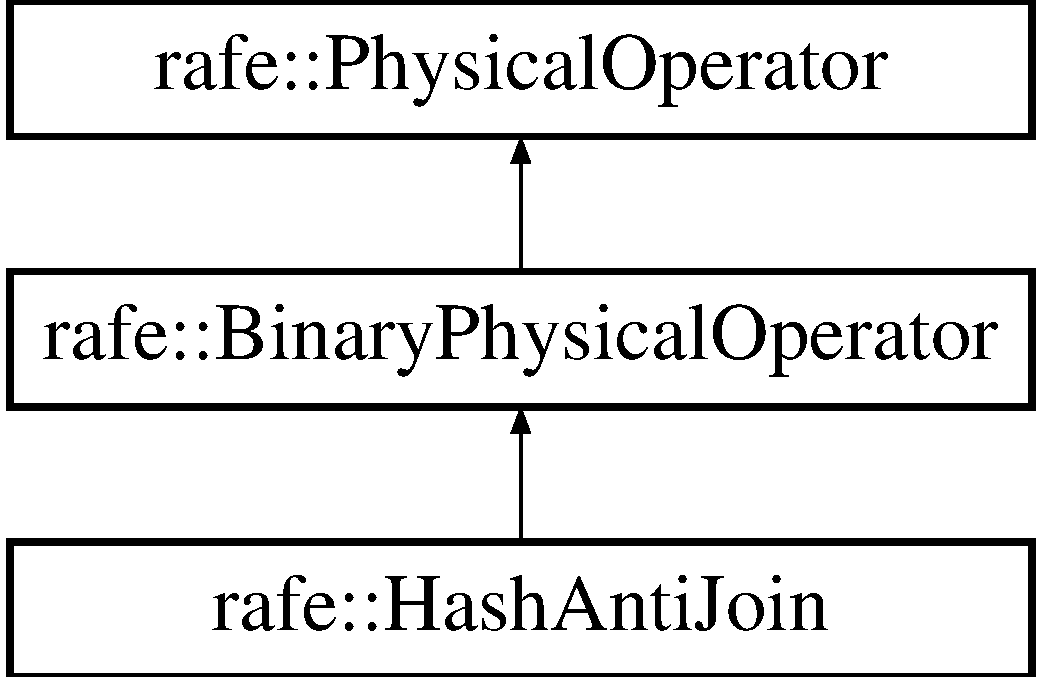
\includegraphics[height=3.000000cm]{classrafe_1_1_hash_anti_join}
\end{center}
\end{figure}
\subsection*{Public Member Functions}
\begin{DoxyCompactItemize}
\item 
\hyperlink{classrafe_1_1_hash_anti_join_a1682f3847d042fe0c3ed5782d94f972d}{Hash\+Anti\+Join} (const std\+::shared\+\_\+ptr$<$ \hyperlink{classrafe_1_1_expression}{Expression} $>$ \&\hyperlink{classrafe_1_1_hash_anti_join_a23275305fdc386ac5cd85a72e3cf35b5}{condition}, const std\+::vector$<$ \hyperlink{classrafe_1_1_column_identifier}{Column\+Identifier} $>$ \&\hyperlink{classrafe_1_1_hash_anti_join_aee96d4c1b6379eddfce548a5ad0733f0}{left\+Part\+Of\+Condition}, const std\+::vector$<$ \hyperlink{classrafe_1_1_column_identifier}{Column\+Identifier} $>$ \&\hyperlink{classrafe_1_1_hash_anti_join_a3d1f9f90ff58e9af2c24cf432a5c8508}{right\+Part\+Of\+Condition})
\item 
void \hyperlink{classrafe_1_1_hash_anti_join_a3df56df88dd2e9280d6243cba23b4ac4}{accept} (\hyperlink{classrafe_1_1_physical_operator_visitor}{Physical\+Operator\+Visitor} \&v)
\end{DoxyCompactItemize}
\subsection*{Public Attributes}
\begin{DoxyCompactItemize}
\item 
std\+::shared\+\_\+ptr$<$ \hyperlink{classrafe_1_1_expression}{Expression} $>$ \hyperlink{classrafe_1_1_hash_anti_join_a23275305fdc386ac5cd85a72e3cf35b5}{condition}
\item 
std\+::vector$<$ \hyperlink{classrafe_1_1_column_identifier}{Column\+Identifier} $>$ \hyperlink{classrafe_1_1_hash_anti_join_aee96d4c1b6379eddfce548a5ad0733f0}{left\+Part\+Of\+Condition}
\item 
std\+::vector$<$ \hyperlink{classrafe_1_1_column_identifier}{Column\+Identifier} $>$ \hyperlink{classrafe_1_1_hash_anti_join_a3d1f9f90ff58e9af2c24cf432a5c8508}{right\+Part\+Of\+Condition}
\end{DoxyCompactItemize}


\subsection{Detailed Description}
Represents hash antijoin physical operator. Operator computes equi join using hash table. First input will be stored in a hash table. 

\subsection{Constructor \& Destructor Documentation}
\hypertarget{classrafe_1_1_hash_anti_join_a1682f3847d042fe0c3ed5782d94f972d}{\index{rafe\+::\+Hash\+Anti\+Join@{rafe\+::\+Hash\+Anti\+Join}!Hash\+Anti\+Join@{Hash\+Anti\+Join}}
\index{Hash\+Anti\+Join@{Hash\+Anti\+Join}!rafe\+::\+Hash\+Anti\+Join@{rafe\+::\+Hash\+Anti\+Join}}
\subsubsection[{Hash\+Anti\+Join}]{\setlength{\rightskip}{0pt plus 5cm}rafe\+::\+Hash\+Anti\+Join\+::\+Hash\+Anti\+Join (
\begin{DoxyParamCaption}
\item[{const std\+::shared\+\_\+ptr$<$ {\bf Expression} $>$ \&}]{condition, }
\item[{const std\+::vector$<$ {\bf Column\+Identifier} $>$ \&}]{left\+Part\+Of\+Condition, }
\item[{const std\+::vector$<$ {\bf Column\+Identifier} $>$ \&}]{right\+Part\+Of\+Condition}
\end{DoxyParamCaption}
)}}\label{classrafe_1_1_hash_anti_join_a1682f3847d042fe0c3ed5782d94f972d}
Creates new instance of \hyperlink{classrafe_1_1_hash_anti_join}{Hash\+Anti\+Join}. 
\begin{DoxyParams}{Parameters}
{\em condition} & -\/ join condition. \\
\hline
{\em left\+Part\+Of\+Condition} & -\/ condition columns from first input. \\
\hline
{\em right\+Part\+Of\+Condition} & -\/ condition columns from second input. \\
\hline
\end{DoxyParams}


\subsection{Member Function Documentation}
\hypertarget{classrafe_1_1_hash_anti_join_a3df56df88dd2e9280d6243cba23b4ac4}{\index{rafe\+::\+Hash\+Anti\+Join@{rafe\+::\+Hash\+Anti\+Join}!accept@{accept}}
\index{accept@{accept}!rafe\+::\+Hash\+Anti\+Join@{rafe\+::\+Hash\+Anti\+Join}}
\subsubsection[{accept}]{\setlength{\rightskip}{0pt plus 5cm}void rafe\+::\+Hash\+Anti\+Join\+::accept (
\begin{DoxyParamCaption}
\item[{{\bf Physical\+Operator\+Visitor} \&}]{v}
\end{DoxyParamCaption}
)\hspace{0.3cm}{\ttfamily [virtual]}}}\label{classrafe_1_1_hash_anti_join_a3df56df88dd2e9280d6243cba23b4ac4}
Method for calling visit\mbox{[}node\mbox{]} on given \hyperlink{classrafe_1_1_physical_operator_visitor}{Physical\+Operator\+Visitor}. 
\begin{DoxyParams}{Parameters}
{\em v} & \hyperlink{classrafe_1_1_physical_operator_visitor}{Physical\+Operator\+Visitor}, on which to call function. \\
\hline
\end{DoxyParams}


Implements \hyperlink{classrafe_1_1_binary_physical_operator_a58ce0a14b970b2c932254419877a2e0e}{rafe\+::\+Binary\+Physical\+Operator}.



\subsection{Member Data Documentation}
\hypertarget{classrafe_1_1_hash_anti_join_a23275305fdc386ac5cd85a72e3cf35b5}{\index{rafe\+::\+Hash\+Anti\+Join@{rafe\+::\+Hash\+Anti\+Join}!condition@{condition}}
\index{condition@{condition}!rafe\+::\+Hash\+Anti\+Join@{rafe\+::\+Hash\+Anti\+Join}}
\subsubsection[{condition}]{\setlength{\rightskip}{0pt plus 5cm}std\+::shared\+\_\+ptr$<${\bf Expression}$>$ rafe\+::\+Hash\+Anti\+Join\+::condition}}\label{classrafe_1_1_hash_anti_join_a23275305fdc386ac5cd85a72e3cf35b5}
Anti join condition. \hypertarget{classrafe_1_1_hash_anti_join_aee96d4c1b6379eddfce548a5ad0733f0}{\index{rafe\+::\+Hash\+Anti\+Join@{rafe\+::\+Hash\+Anti\+Join}!left\+Part\+Of\+Condition@{left\+Part\+Of\+Condition}}
\index{left\+Part\+Of\+Condition@{left\+Part\+Of\+Condition}!rafe\+::\+Hash\+Anti\+Join@{rafe\+::\+Hash\+Anti\+Join}}
\subsubsection[{left\+Part\+Of\+Condition}]{\setlength{\rightskip}{0pt plus 5cm}std\+::vector$<${\bf Column\+Identifier}$>$ rafe\+::\+Hash\+Anti\+Join\+::left\+Part\+Of\+Condition}}\label{classrafe_1_1_hash_anti_join_aee96d4c1b6379eddfce548a5ad0733f0}
Stores columns from left input, which belongs to condition. \hypertarget{classrafe_1_1_hash_anti_join_a3d1f9f90ff58e9af2c24cf432a5c8508}{\index{rafe\+::\+Hash\+Anti\+Join@{rafe\+::\+Hash\+Anti\+Join}!right\+Part\+Of\+Condition@{right\+Part\+Of\+Condition}}
\index{right\+Part\+Of\+Condition@{right\+Part\+Of\+Condition}!rafe\+::\+Hash\+Anti\+Join@{rafe\+::\+Hash\+Anti\+Join}}
\subsubsection[{right\+Part\+Of\+Condition}]{\setlength{\rightskip}{0pt plus 5cm}std\+::vector$<${\bf Column\+Identifier}$>$ rafe\+::\+Hash\+Anti\+Join\+::right\+Part\+Of\+Condition}}\label{classrafe_1_1_hash_anti_join_a3d1f9f90ff58e9af2c24cf432a5c8508}
Stores columns from right input, which belongs to condition. 

The documentation for this class was generated from the following files\+:\begin{DoxyCompactItemize}
\item 
C\+:/\+Users/\+Marcel/\+Documents/\+Visual Studio 2012/\+Projects/\+Relational\+Query\+Evaluator/\+Relational\+Query\+Evaluator/Physical\+Operator.\+h\item 
C\+:/\+Users/\+Marcel/\+Documents/\+Visual Studio 2012/\+Projects/\+Relational\+Query\+Evaluator/\+Relational\+Query\+Evaluator/Physical\+Operator.\+cpp\end{DoxyCompactItemize}

\hypertarget{classrafe_1_1_hash_group}{\section{rafe\+:\+:Hash\+Group Class Reference}
\label{classrafe_1_1_hash_group}\index{rafe\+::\+Hash\+Group@{rafe\+::\+Hash\+Group}}
}


{\ttfamily \#include $<$Physical\+Operator.\+h$>$}

Inheritance diagram for rafe\+:\+:Hash\+Group\+:\begin{figure}[H]
\begin{center}
\leavevmode
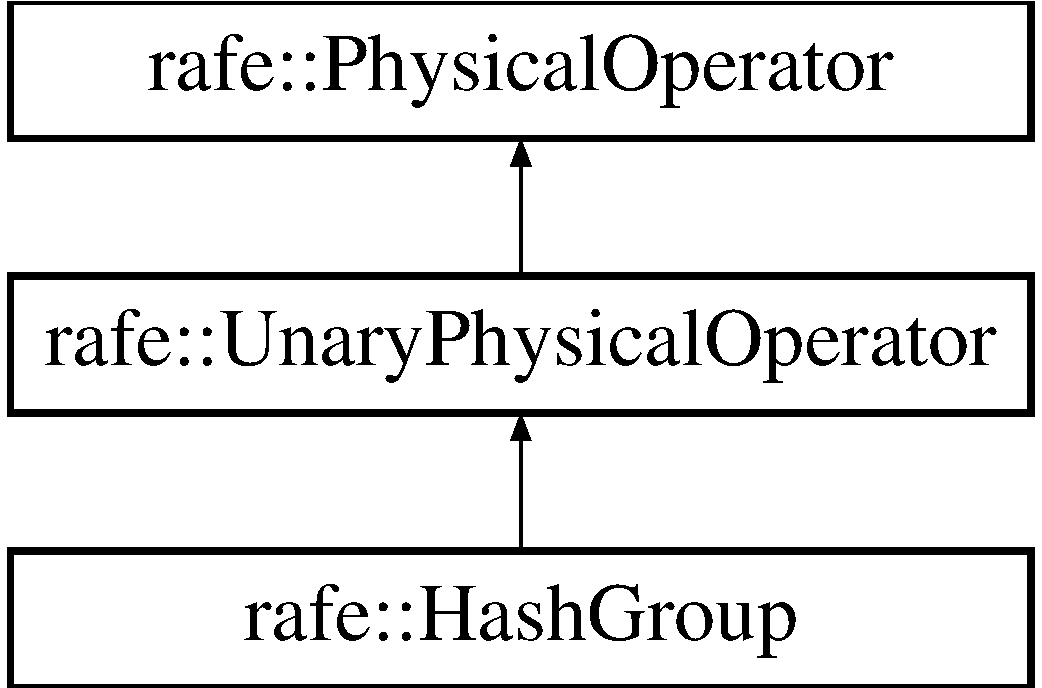
\includegraphics[height=3.000000cm]{classrafe_1_1_hash_group}
\end{center}
\end{figure}
\subsection*{Public Member Functions}
\begin{DoxyCompactItemize}
\item 
\hyperlink{classrafe_1_1_hash_group_af175c50e75d33c109d3c2413501932b1}{Hash\+Group} (const std\+::vector$<$ \hyperlink{classrafe_1_1_group_column}{Group\+Column} $>$ \&\hyperlink{classrafe_1_1_hash_group_a440af6cd151c376aefb5385bbac54cb8}{group\+Columns}, const std\+::vector$<$ \hyperlink{classrafe_1_1_agregate_function}{Agregate\+Function} $>$ \&\hyperlink{classrafe_1_1_hash_group_a26ed49743b63ae86b803e9fe725e72c1}{agregate\+Functions})
\item 
void \hyperlink{classrafe_1_1_hash_group_a91335ef36a07f6ab099785073e16786b}{accept} (\hyperlink{classrafe_1_1_physical_operator_visitor}{Physical\+Operator\+Visitor} \&v)
\end{DoxyCompactItemize}
\subsection*{Public Attributes}
\begin{DoxyCompactItemize}
\item 
std\+::vector$<$ \hyperlink{classrafe_1_1_group_column}{Group\+Column} $>$ \hyperlink{classrafe_1_1_hash_group_a440af6cd151c376aefb5385bbac54cb8}{group\+Columns}
\item 
std\+::vector$<$ \hyperlink{classrafe_1_1_agregate_function}{Agregate\+Function} $>$ \hyperlink{classrafe_1_1_hash_group_a26ed49743b63ae86b803e9fe725e72c1}{agregate\+Functions}
\end{DoxyCompactItemize}


\subsection{Detailed Description}
Represent hash group algorithm. 

\subsection{Constructor \& Destructor Documentation}
\hypertarget{classrafe_1_1_hash_group_af175c50e75d33c109d3c2413501932b1}{\index{rafe\+::\+Hash\+Group@{rafe\+::\+Hash\+Group}!Hash\+Group@{Hash\+Group}}
\index{Hash\+Group@{Hash\+Group}!rafe\+::\+Hash\+Group@{rafe\+::\+Hash\+Group}}
\subsubsection[{Hash\+Group}]{\setlength{\rightskip}{0pt plus 5cm}rafe\+::\+Hash\+Group\+::\+Hash\+Group (
\begin{DoxyParamCaption}
\item[{const std\+::vector$<$ {\bf Group\+Column} $>$ \&}]{group\+Columns, }
\item[{const std\+::vector$<$ {\bf Agregate\+Function} $>$ \&}]{agregate\+Functions}
\end{DoxyParamCaption}
)}}\label{classrafe_1_1_hash_group_af175c50e75d33c109d3c2413501932b1}
Creates new instance of \hyperlink{classrafe_1_1_hash_group}{Hash\+Group}. 
\begin{DoxyParams}{Parameters}
{\em group\+Columns} & -\/ group by columns. \\
\hline
{\em agregate\+Functions} & -\/ information about agreggate functions. \\
\hline
\end{DoxyParams}


\subsection{Member Function Documentation}
\hypertarget{classrafe_1_1_hash_group_a91335ef36a07f6ab099785073e16786b}{\index{rafe\+::\+Hash\+Group@{rafe\+::\+Hash\+Group}!accept@{accept}}
\index{accept@{accept}!rafe\+::\+Hash\+Group@{rafe\+::\+Hash\+Group}}
\subsubsection[{accept}]{\setlength{\rightskip}{0pt plus 5cm}void rafe\+::\+Hash\+Group\+::accept (
\begin{DoxyParamCaption}
\item[{{\bf Physical\+Operator\+Visitor} \&}]{v}
\end{DoxyParamCaption}
)\hspace{0.3cm}{\ttfamily [virtual]}}}\label{classrafe_1_1_hash_group_a91335ef36a07f6ab099785073e16786b}
Method for calling visit\mbox{[}node\mbox{]} on given \hyperlink{classrafe_1_1_physical_operator_visitor}{Physical\+Operator\+Visitor}. 
\begin{DoxyParams}{Parameters}
{\em v} & \hyperlink{classrafe_1_1_physical_operator_visitor}{Physical\+Operator\+Visitor}, on which to call function. \\
\hline
\end{DoxyParams}


Implements \hyperlink{classrafe_1_1_unary_physical_operator_a56a160698a78f8a0aa44e47e0804f45e}{rafe\+::\+Unary\+Physical\+Operator}.



\subsection{Member Data Documentation}
\hypertarget{classrafe_1_1_hash_group_a26ed49743b63ae86b803e9fe725e72c1}{\index{rafe\+::\+Hash\+Group@{rafe\+::\+Hash\+Group}!agregate\+Functions@{agregate\+Functions}}
\index{agregate\+Functions@{agregate\+Functions}!rafe\+::\+Hash\+Group@{rafe\+::\+Hash\+Group}}
\subsubsection[{agregate\+Functions}]{\setlength{\rightskip}{0pt plus 5cm}std\+::vector$<${\bf Agregate\+Function}$>$ rafe\+::\+Hash\+Group\+::agregate\+Functions}}\label{classrafe_1_1_hash_group_a26ed49743b63ae86b803e9fe725e72c1}
Information about agreggate functions. \hypertarget{classrafe_1_1_hash_group_a440af6cd151c376aefb5385bbac54cb8}{\index{rafe\+::\+Hash\+Group@{rafe\+::\+Hash\+Group}!group\+Columns@{group\+Columns}}
\index{group\+Columns@{group\+Columns}!rafe\+::\+Hash\+Group@{rafe\+::\+Hash\+Group}}
\subsubsection[{group\+Columns}]{\setlength{\rightskip}{0pt plus 5cm}std\+::vector$<${\bf Group\+Column}$>$ rafe\+::\+Hash\+Group\+::group\+Columns}}\label{classrafe_1_1_hash_group_a440af6cd151c376aefb5385bbac54cb8}
\hyperlink{classrafe_1_1_group}{Group} by columns. 

The documentation for this class was generated from the following files\+:\begin{DoxyCompactItemize}
\item 
C\+:/\+Users/\+Marcel/\+Documents/\+Visual Studio 2012/\+Projects/\+Relational\+Query\+Evaluator/\+Relational\+Query\+Evaluator/Physical\+Operator.\+h\item 
C\+:/\+Users/\+Marcel/\+Documents/\+Visual Studio 2012/\+Projects/\+Relational\+Query\+Evaluator/\+Relational\+Query\+Evaluator/Physical\+Operator.\+cpp\end{DoxyCompactItemize}

\hypertarget{classrafe_1_1_hash_join}{\section{rafe\+:\+:Hash\+Join Class Reference}
\label{classrafe_1_1_hash_join}\index{rafe\+::\+Hash\+Join@{rafe\+::\+Hash\+Join}}
}


{\ttfamily \#include $<$Physical\+Operator.\+h$>$}

Inheritance diagram for rafe\+:\+:Hash\+Join\+:\begin{figure}[H]
\begin{center}
\leavevmode
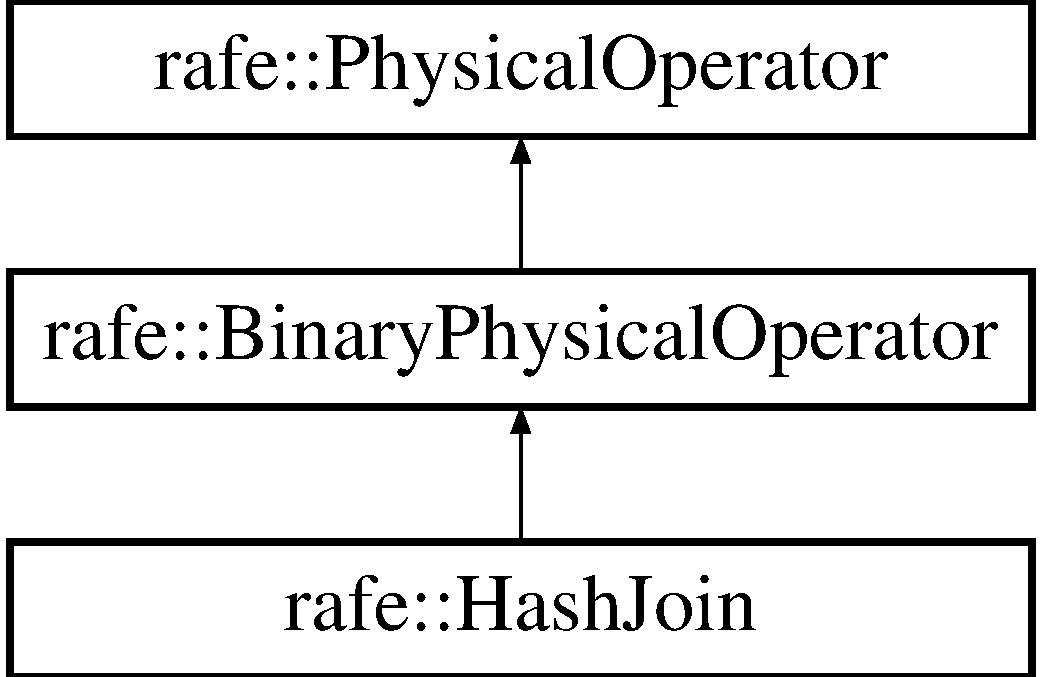
\includegraphics[height=3.000000cm]{classrafe_1_1_hash_join}
\end{center}
\end{figure}
\subsection*{Public Member Functions}
\begin{DoxyCompactItemize}
\item 
\hyperlink{classrafe_1_1_hash_join_a07a2174c405518eca64c4370a7741429}{Hash\+Join} (const std\+::shared\+\_\+ptr$<$ \hyperlink{classrafe_1_1_expression}{Expression} $>$ \&\hyperlink{classrafe_1_1_hash_join_a0642b38448cb547c6b6a118002bc0dd8}{condition}, const std\+::vector$<$ \hyperlink{classrafe_1_1_column_identifier}{Column\+Identifier} $>$ \&\hyperlink{classrafe_1_1_hash_join_a7cc0d8d90cd314e40a0cc467954c91d1}{left\+Part\+Of\+Condition}, const std\+::vector$<$ \hyperlink{classrafe_1_1_column_identifier}{Column\+Identifier} $>$ \&\hyperlink{classrafe_1_1_hash_join_a8d6f385e17aa74f96d4ca7e66f09fac8}{right\+Part\+Of\+Condition})
\item 
void \hyperlink{classrafe_1_1_hash_join_abd86be090582ddf7e87ac7d3dd2f60a7}{accept} (\hyperlink{classrafe_1_1_physical_operator_visitor}{Physical\+Operator\+Visitor} \&v)
\end{DoxyCompactItemize}
\subsection*{Public Attributes}
\begin{DoxyCompactItemize}
\item 
std\+::shared\+\_\+ptr$<$ \hyperlink{classrafe_1_1_expression}{Expression} $>$ \hyperlink{classrafe_1_1_hash_join_a0642b38448cb547c6b6a118002bc0dd8}{condition}
\item 
std\+::vector$<$ \hyperlink{classrafe_1_1_column_identifier}{Column\+Identifier} $>$ \hyperlink{classrafe_1_1_hash_join_a7cc0d8d90cd314e40a0cc467954c91d1}{left\+Part\+Of\+Condition}
\item 
std\+::vector$<$ \hyperlink{classrafe_1_1_column_identifier}{Column\+Identifier} $>$ \hyperlink{classrafe_1_1_hash_join_a8d6f385e17aa74f96d4ca7e66f09fac8}{right\+Part\+Of\+Condition}
\end{DoxyCompactItemize}


\subsection{Detailed Description}
Represents hash join physical operator. Operator computes equi join using hash table. First input will be stored in hash table. 

\subsection{Constructor \& Destructor Documentation}
\hypertarget{classrafe_1_1_hash_join_a07a2174c405518eca64c4370a7741429}{\index{rafe\+::\+Hash\+Join@{rafe\+::\+Hash\+Join}!Hash\+Join@{Hash\+Join}}
\index{Hash\+Join@{Hash\+Join}!rafe\+::\+Hash\+Join@{rafe\+::\+Hash\+Join}}
\subsubsection[{Hash\+Join}]{\setlength{\rightskip}{0pt plus 5cm}rafe\+::\+Hash\+Join\+::\+Hash\+Join (
\begin{DoxyParamCaption}
\item[{const std\+::shared\+\_\+ptr$<$ {\bf Expression} $>$ \&}]{condition, }
\item[{const std\+::vector$<$ {\bf Column\+Identifier} $>$ \&}]{left\+Part\+Of\+Condition, }
\item[{const std\+::vector$<$ {\bf Column\+Identifier} $>$ \&}]{right\+Part\+Of\+Condition}
\end{DoxyParamCaption}
)}}\label{classrafe_1_1_hash_join_a07a2174c405518eca64c4370a7741429}
Creates new instance of \hyperlink{classrafe_1_1_hash_join}{Hash\+Join}. 
\begin{DoxyParams}{Parameters}
{\em condition} & -\/ join condition. \\
\hline
{\em left\+Part\+Of\+Condition} & -\/ condition columns from first input \\
\hline
{\em right\+Part\+Of\+Condition} & -\/ condition columns from second input \\
\hline
\end{DoxyParams}


\subsection{Member Function Documentation}
\hypertarget{classrafe_1_1_hash_join_abd86be090582ddf7e87ac7d3dd2f60a7}{\index{rafe\+::\+Hash\+Join@{rafe\+::\+Hash\+Join}!accept@{accept}}
\index{accept@{accept}!rafe\+::\+Hash\+Join@{rafe\+::\+Hash\+Join}}
\subsubsection[{accept}]{\setlength{\rightskip}{0pt plus 5cm}void rafe\+::\+Hash\+Join\+::accept (
\begin{DoxyParamCaption}
\item[{{\bf Physical\+Operator\+Visitor} \&}]{v}
\end{DoxyParamCaption}
)\hspace{0.3cm}{\ttfamily [virtual]}}}\label{classrafe_1_1_hash_join_abd86be090582ddf7e87ac7d3dd2f60a7}
Method for calling visit\mbox{[}node\mbox{]} on given \hyperlink{classrafe_1_1_physical_operator_visitor}{Physical\+Operator\+Visitor}. 
\begin{DoxyParams}{Parameters}
{\em v} & \hyperlink{classrafe_1_1_physical_operator_visitor}{Physical\+Operator\+Visitor}, on which to call function. \\
\hline
\end{DoxyParams}


Implements \hyperlink{classrafe_1_1_binary_physical_operator_a58ce0a14b970b2c932254419877a2e0e}{rafe\+::\+Binary\+Physical\+Operator}.



\subsection{Member Data Documentation}
\hypertarget{classrafe_1_1_hash_join_a0642b38448cb547c6b6a118002bc0dd8}{\index{rafe\+::\+Hash\+Join@{rafe\+::\+Hash\+Join}!condition@{condition}}
\index{condition@{condition}!rafe\+::\+Hash\+Join@{rafe\+::\+Hash\+Join}}
\subsubsection[{condition}]{\setlength{\rightskip}{0pt plus 5cm}std\+::shared\+\_\+ptr$<${\bf Expression}$>$ rafe\+::\+Hash\+Join\+::condition}}\label{classrafe_1_1_hash_join_a0642b38448cb547c6b6a118002bc0dd8}
\hyperlink{classrafe_1_1_join}{Join} condition. \hypertarget{classrafe_1_1_hash_join_a7cc0d8d90cd314e40a0cc467954c91d1}{\index{rafe\+::\+Hash\+Join@{rafe\+::\+Hash\+Join}!left\+Part\+Of\+Condition@{left\+Part\+Of\+Condition}}
\index{left\+Part\+Of\+Condition@{left\+Part\+Of\+Condition}!rafe\+::\+Hash\+Join@{rafe\+::\+Hash\+Join}}
\subsubsection[{left\+Part\+Of\+Condition}]{\setlength{\rightskip}{0pt plus 5cm}std\+::vector$<${\bf Column\+Identifier}$>$ rafe\+::\+Hash\+Join\+::left\+Part\+Of\+Condition}}\label{classrafe_1_1_hash_join_a7cc0d8d90cd314e40a0cc467954c91d1}
Stores columns from left input, which belongs to condition. \hypertarget{classrafe_1_1_hash_join_a8d6f385e17aa74f96d4ca7e66f09fac8}{\index{rafe\+::\+Hash\+Join@{rafe\+::\+Hash\+Join}!right\+Part\+Of\+Condition@{right\+Part\+Of\+Condition}}
\index{right\+Part\+Of\+Condition@{right\+Part\+Of\+Condition}!rafe\+::\+Hash\+Join@{rafe\+::\+Hash\+Join}}
\subsubsection[{right\+Part\+Of\+Condition}]{\setlength{\rightskip}{0pt plus 5cm}std\+::vector$<${\bf Column\+Identifier}$>$ rafe\+::\+Hash\+Join\+::right\+Part\+Of\+Condition}}\label{classrafe_1_1_hash_join_a8d6f385e17aa74f96d4ca7e66f09fac8}
Stores columns from right input, which belongs to condition. 

The documentation for this class was generated from the following files\+:\begin{DoxyCompactItemize}
\item 
C\+:/\+Users/\+Marcel/\+Documents/\+Visual Studio 2012/\+Projects/\+Relational\+Query\+Evaluator/\+Relational\+Query\+Evaluator/Physical\+Operator.\+h\item 
C\+:/\+Users/\+Marcel/\+Documents/\+Visual Studio 2012/\+Projects/\+Relational\+Query\+Evaluator/\+Relational\+Query\+Evaluator/Physical\+Operator.\+cpp\end{DoxyCompactItemize}

\hypertarget{classrafe_1_1_index}{\section{rafe\+:\+:Index Class Reference}
\label{classrafe_1_1_index}\index{rafe\+::\+Index@{rafe\+::\+Index}}
}


{\ttfamily \#include $<$Algebra\+Structures.\+h$>$}

\subsection*{Public Member Functions}
\begin{DoxyCompactItemize}
\item 
std\+::string \hyperlink{classrafe_1_1_index_afa130a8610ea8a063d1ffb63f03de3d4}{to\+String} ()
\end{DoxyCompactItemize}
\subsection*{Public Attributes}
\begin{DoxyCompactItemize}
\item 
Index\+Type \hyperlink{classrafe_1_1_index_ab51a314af4e6fcda600f72b2ca5a6851}{type}
\item 
std\+::string \hyperlink{classrafe_1_1_index_adfba6ba7d75003d44df8b92d6e232346}{name}
\item 
std\+::vector$<$ \hyperlink{classrafe_1_1_sort_parameter}{Sort\+Parameter} $>$ \hyperlink{classrafe_1_1_index_a74cf2aef59f22a7ef0175b59908bd3b2}{columns}
\end{DoxyCompactItemize}


\subsection{Detailed Description}
Structure storing information about index on table. 

\subsection{Member Function Documentation}
\hypertarget{classrafe_1_1_index_afa130a8610ea8a063d1ffb63f03de3d4}{\index{rafe\+::\+Index@{rafe\+::\+Index}!to\+String@{to\+String}}
\index{to\+String@{to\+String}!rafe\+::\+Index@{rafe\+::\+Index}}
\subsubsection[{to\+String}]{\setlength{\rightskip}{0pt plus 5cm}string rafe\+::\+Index\+::to\+String (
\begin{DoxyParamCaption}
{}
\end{DoxyParamCaption}
)}}\label{classrafe_1_1_index_afa130a8610ea8a063d1ffb63f03de3d4}
\begin{DoxyReturn}{Returns}
String representation of this class. 
\end{DoxyReturn}


\subsection{Member Data Documentation}
\hypertarget{classrafe_1_1_index_a74cf2aef59f22a7ef0175b59908bd3b2}{\index{rafe\+::\+Index@{rafe\+::\+Index}!columns@{columns}}
\index{columns@{columns}!rafe\+::\+Index@{rafe\+::\+Index}}
\subsubsection[{columns}]{\setlength{\rightskip}{0pt plus 5cm}std\+::vector$<${\bf Sort\+Parameter}$>$ rafe\+::\+Index\+::columns}}\label{classrafe_1_1_index_a74cf2aef59f22a7ef0175b59908bd3b2}
\hyperlink{classrafe_1_1_index}{Index} columns with their sort order. \hypertarget{classrafe_1_1_index_adfba6ba7d75003d44df8b92d6e232346}{\index{rafe\+::\+Index@{rafe\+::\+Index}!name@{name}}
\index{name@{name}!rafe\+::\+Index@{rafe\+::\+Index}}
\subsubsection[{name}]{\setlength{\rightskip}{0pt plus 5cm}std\+::string rafe\+::\+Index\+::name}}\label{classrafe_1_1_index_adfba6ba7d75003d44df8b92d6e232346}
\hyperlink{classrafe_1_1_index}{Index} name. \hypertarget{classrafe_1_1_index_ab51a314af4e6fcda600f72b2ca5a6851}{\index{rafe\+::\+Index@{rafe\+::\+Index}!type@{type}}
\index{type@{type}!rafe\+::\+Index@{rafe\+::\+Index}}
\subsubsection[{type}]{\setlength{\rightskip}{0pt plus 5cm}Index\+Type rafe\+::\+Index\+::type}}\label{classrafe_1_1_index_ab51a314af4e6fcda600f72b2ca5a6851}
Type of index\+: clustered or unclustered. 

The documentation for this class was generated from the following files\+:\begin{DoxyCompactItemize}
\item 
C\+:/\+Users/\+Marcel/\+Documents/\+Visual Studio 2012/\+Projects/\+Relational\+Query\+Evaluator/\+Relational\+Query\+Evaluator/Algebra\+Structures.\+h\item 
C\+:/\+Users/\+Marcel/\+Documents/\+Visual Studio 2012/\+Projects/\+Relational\+Query\+Evaluator/\+Relational\+Query\+Evaluator/Algebra\+Structures.\+cpp\end{DoxyCompactItemize}

\hypertarget{classrafe_1_1_index_scan}{\section{rafe\+:\+:Index\+Scan Class Reference}
\label{classrafe_1_1_index_scan}\index{rafe\+::\+Index\+Scan@{rafe\+::\+Index\+Scan}}
}


{\ttfamily \#include $<$Physical\+Operator.\+h$>$}

Inheritance diagram for rafe\+:\+:Index\+Scan\+:\begin{figure}[H]
\begin{center}
\leavevmode
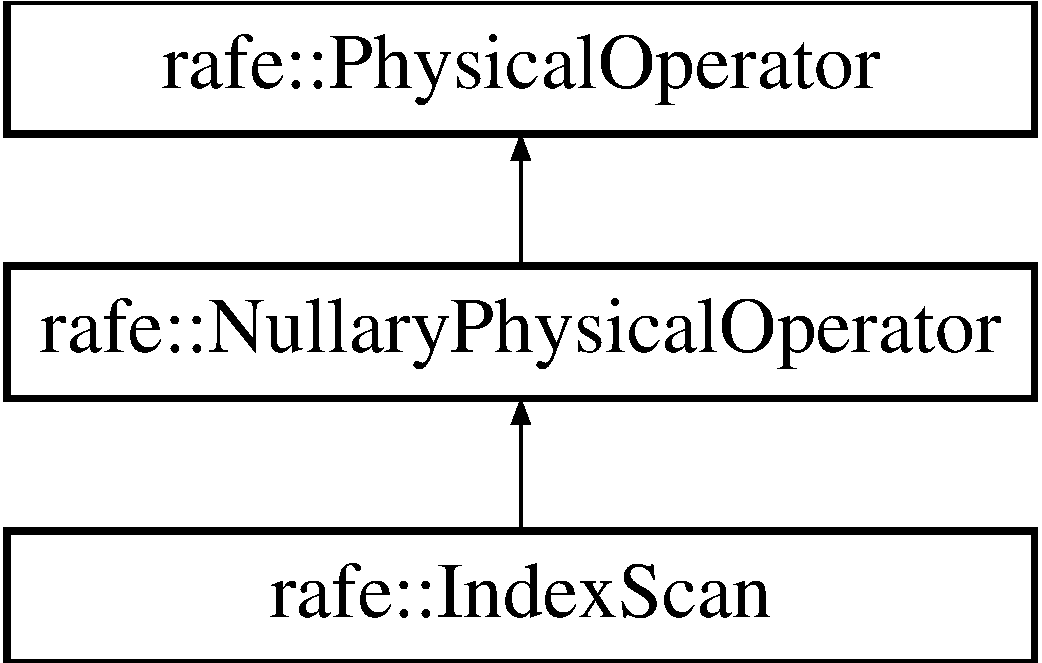
\includegraphics[height=3.000000cm]{classrafe_1_1_index_scan}
\end{center}
\end{figure}
\subsection*{Public Member Functions}
\begin{DoxyCompactItemize}
\item 
\hyperlink{classrafe_1_1_index_scan_acda9bef1fc1996fa1a51dd4965c902c1}{Index\+Scan} (const std\+::string \&name, const std\+::shared\+\_\+ptr$<$ \hyperlink{classrafe_1_1_expression}{Expression} $>$ \&\hyperlink{classrafe_1_1_index_scan_a3ea0ae237e08c4a601529929f6d80052}{condition}, const \hyperlink{classrafe_1_1_index}{Index} \&\hyperlink{classrafe_1_1_index_scan_a95bd35c11302e772572cb37df93cc3a7}{index})
\item 
void \hyperlink{classrafe_1_1_index_scan_a5e4e26317258097176b3b3b241653302}{accept} (\hyperlink{classrafe_1_1_physical_operator_visitor}{Physical\+Operator\+Visitor} \&v)
\end{DoxyCompactItemize}
\subsection*{Public Attributes}
\begin{DoxyCompactItemize}
\item 
std\+::string \hyperlink{classrafe_1_1_index_scan_a10d1f881994a96dee8e9e29f367626e9}{table\+Name}
\item 
std\+::shared\+\_\+ptr$<$ \hyperlink{classrafe_1_1_expression}{Expression} $>$ \hyperlink{classrafe_1_1_index_scan_a3ea0ae237e08c4a601529929f6d80052}{condition}
\item 
\hyperlink{classrafe_1_1_index}{Index} \hyperlink{classrafe_1_1_index_scan_a95bd35c11302e772572cb37df93cc3a7}{index}
\end{DoxyCompactItemize}


\subsection{Detailed Description}
Represents operator, which reads part of the table using index. 

\subsection{Constructor \& Destructor Documentation}
\hypertarget{classrafe_1_1_index_scan_acda9bef1fc1996fa1a51dd4965c902c1}{\index{rafe\+::\+Index\+Scan@{rafe\+::\+Index\+Scan}!Index\+Scan@{Index\+Scan}}
\index{Index\+Scan@{Index\+Scan}!rafe\+::\+Index\+Scan@{rafe\+::\+Index\+Scan}}
\subsubsection[{Index\+Scan}]{\setlength{\rightskip}{0pt plus 5cm}rafe\+::\+Index\+Scan\+::\+Index\+Scan (
\begin{DoxyParamCaption}
\item[{const std\+::string \&}]{name, }
\item[{const std\+::shared\+\_\+ptr$<$ {\bf Expression} $>$ \&}]{condition, }
\item[{const {\bf Index} \&}]{index}
\end{DoxyParamCaption}
)}}\label{classrafe_1_1_index_scan_acda9bef1fc1996fa1a51dd4965c902c1}
Creates new instance of \hyperlink{classrafe_1_1_index_scan}{Index\+Scan}. 
\begin{DoxyParams}{Parameters}
{\em name} & of table to read. \\
\hline
{\em condition} & to apply while reading. \\
\hline
{\em index} & -\/ index to user for reading. \\
\hline
\end{DoxyParams}


\subsection{Member Function Documentation}
\hypertarget{classrafe_1_1_index_scan_a5e4e26317258097176b3b3b241653302}{\index{rafe\+::\+Index\+Scan@{rafe\+::\+Index\+Scan}!accept@{accept}}
\index{accept@{accept}!rafe\+::\+Index\+Scan@{rafe\+::\+Index\+Scan}}
\subsubsection[{accept}]{\setlength{\rightskip}{0pt plus 5cm}void rafe\+::\+Index\+Scan\+::accept (
\begin{DoxyParamCaption}
\item[{{\bf Physical\+Operator\+Visitor} \&}]{v}
\end{DoxyParamCaption}
)\hspace{0.3cm}{\ttfamily [virtual]}}}\label{classrafe_1_1_index_scan_a5e4e26317258097176b3b3b241653302}
Method for calling visit\mbox{[}node\mbox{]} on given \hyperlink{classrafe_1_1_physical_operator_visitor}{Physical\+Operator\+Visitor}. 
\begin{DoxyParams}{Parameters}
{\em v} & \hyperlink{classrafe_1_1_physical_operator_visitor}{Physical\+Operator\+Visitor}, on which to call function. \\
\hline
\end{DoxyParams}


Implements \hyperlink{classrafe_1_1_nullary_physical_operator_a0810fc4b368521ebe847fa48fcdcf948}{rafe\+::\+Nullary\+Physical\+Operator}.



\subsection{Member Data Documentation}
\hypertarget{classrafe_1_1_index_scan_a3ea0ae237e08c4a601529929f6d80052}{\index{rafe\+::\+Index\+Scan@{rafe\+::\+Index\+Scan}!condition@{condition}}
\index{condition@{condition}!rafe\+::\+Index\+Scan@{rafe\+::\+Index\+Scan}}
\subsubsection[{condition}]{\setlength{\rightskip}{0pt plus 5cm}std\+::shared\+\_\+ptr$<${\bf Expression}$>$ rafe\+::\+Index\+Scan\+::condition}}\label{classrafe_1_1_index_scan_a3ea0ae237e08c4a601529929f6d80052}
Condition to apply while reading. \hypertarget{classrafe_1_1_index_scan_a95bd35c11302e772572cb37df93cc3a7}{\index{rafe\+::\+Index\+Scan@{rafe\+::\+Index\+Scan}!index@{index}}
\index{index@{index}!rafe\+::\+Index\+Scan@{rafe\+::\+Index\+Scan}}
\subsubsection[{index}]{\setlength{\rightskip}{0pt plus 5cm}{\bf Index} rafe\+::\+Index\+Scan\+::index}}\label{classrafe_1_1_index_scan_a95bd35c11302e772572cb37df93cc3a7}
\hyperlink{classrafe_1_1_table}{Table} index to use. \hypertarget{classrafe_1_1_index_scan_a10d1f881994a96dee8e9e29f367626e9}{\index{rafe\+::\+Index\+Scan@{rafe\+::\+Index\+Scan}!table\+Name@{table\+Name}}
\index{table\+Name@{table\+Name}!rafe\+::\+Index\+Scan@{rafe\+::\+Index\+Scan}}
\subsubsection[{table\+Name}]{\setlength{\rightskip}{0pt plus 5cm}std\+::string rafe\+::\+Index\+Scan\+::table\+Name}}\label{classrafe_1_1_index_scan_a10d1f881994a96dee8e9e29f367626e9}
\hyperlink{classrafe_1_1_table}{Table} to read. 

The documentation for this class was generated from the following files\+:\begin{DoxyCompactItemize}
\item 
C\+:/\+Users/\+Marcel/\+Documents/\+Visual Studio 2012/\+Projects/\+Relational\+Query\+Evaluator/\+Relational\+Query\+Evaluator/Physical\+Operator.\+h\item 
C\+:/\+Users/\+Marcel/\+Documents/\+Visual Studio 2012/\+Projects/\+Relational\+Query\+Evaluator/\+Relational\+Query\+Evaluator/Physical\+Operator.\+cpp\end{DoxyCompactItemize}

\hypertarget{classrafe_1_1_join}{\section{rafe\+:\+:Join Class Reference}
\label{classrafe_1_1_join}\index{rafe\+::\+Join@{rafe\+::\+Join}}
}


{\ttfamily \#include $<$Algebra.\+h$>$}

Inheritance diagram for rafe\+:\+:Join\+:\begin{figure}[H]
\begin{center}
\leavevmode
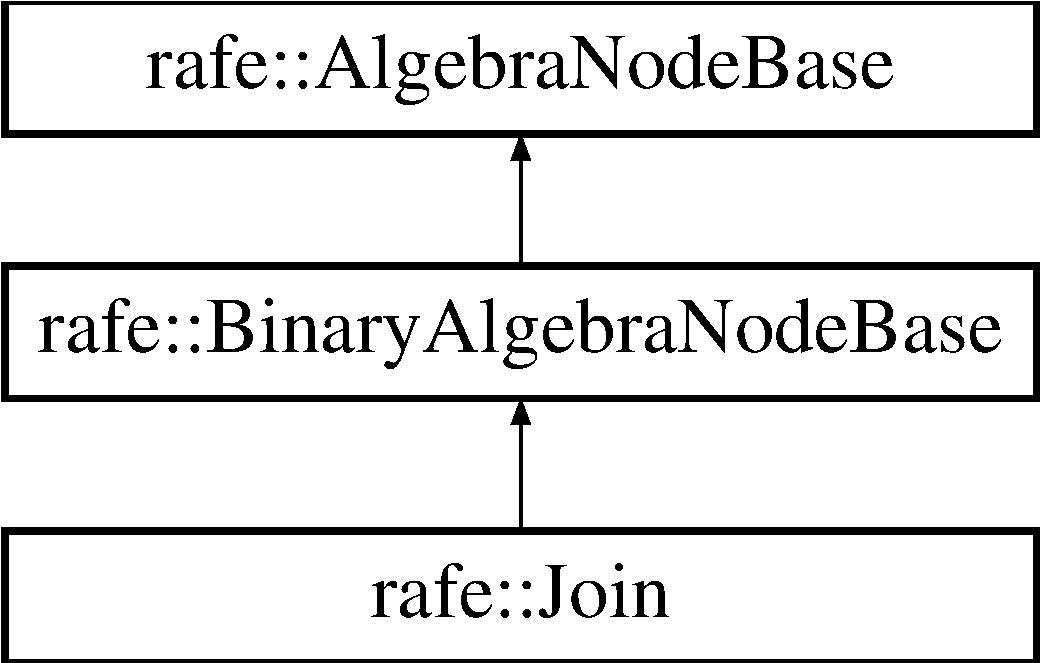
\includegraphics[height=3.000000cm]{classrafe_1_1_join}
\end{center}
\end{figure}
\subsection*{Public Member Functions}
\begin{DoxyCompactItemize}
\item 
\hyperlink{classrafe_1_1_join_a5fb8f205a20616da647526b62d7e75d4}{Join} (D\+O\+M\+Element $\ast$element)
\item 
void \hyperlink{classrafe_1_1_join_a980b203f7b31b44fc564c996fcf28e98}{accept} (\hyperlink{classrafe_1_1_algebra_visitor}{Algebra\+Visitor} \&v)
\end{DoxyCompactItemize}
\subsection*{Public Attributes}
\begin{DoxyCompactItemize}
\item 
std\+::shared\+\_\+ptr$<$ \hyperlink{classrafe_1_1_expression}{Expression} $>$ \hyperlink{classrafe_1_1_join_a77107b49ea977bec841828886bbad392}{condition}
\item 
std\+::vector$<$ \hyperlink{classrafe_1_1_join_column_info}{Join\+Column\+Info} $>$ \hyperlink{classrafe_1_1_join_aea03cf876f6e1b4eab27c07492e103bf}{output\+Join\+Columns}
\end{DoxyCompactItemize}


\subsection{Detailed Description}
Represents binary join operation. 

\subsection{Constructor \& Destructor Documentation}
\hypertarget{classrafe_1_1_join_a5fb8f205a20616da647526b62d7e75d4}{\index{rafe\+::\+Join@{rafe\+::\+Join}!Join@{Join}}
\index{Join@{Join}!rafe\+::\+Join@{rafe\+::\+Join}}
\subsubsection[{Join}]{\setlength{\rightskip}{0pt plus 5cm}rafe\+::\+Join\+::\+Join (
\begin{DoxyParamCaption}
\item[{D\+O\+M\+Element $\ast$}]{element}
\end{DoxyParamCaption}
)}}\label{classrafe_1_1_join_a5fb8f205a20616da647526b62d7e75d4}
Creates the instance of \hyperlink{classrafe_1_1_join}{Join}. 
\begin{DoxyParams}{Parameters}
{\em element} & representing input node. \\
\hline
\end{DoxyParams}


\subsection{Member Function Documentation}
\hypertarget{classrafe_1_1_join_a980b203f7b31b44fc564c996fcf28e98}{\index{rafe\+::\+Join@{rafe\+::\+Join}!accept@{accept}}
\index{accept@{accept}!rafe\+::\+Join@{rafe\+::\+Join}}
\subsubsection[{accept}]{\setlength{\rightskip}{0pt plus 5cm}void rafe\+::\+Join\+::accept (
\begin{DoxyParamCaption}
\item[{{\bf Algebra\+Visitor} \&}]{v}
\end{DoxyParamCaption}
)\hspace{0.3cm}{\ttfamily [virtual]}}}\label{classrafe_1_1_join_a980b203f7b31b44fc564c996fcf28e98}
Method for calling visit\mbox{[}node\mbox{]} on given \hyperlink{classrafe_1_1_algebra_visitor}{Algebra\+Visitor}. 
\begin{DoxyParams}{Parameters}
{\em v} & \hyperlink{classrafe_1_1_algebra_visitor}{Algebra\+Visitor} which to call function on \\
\hline
\end{DoxyParams}


Implements \hyperlink{classrafe_1_1_binary_algebra_node_base_a0c9c2fdbd7062bf0bf4587b9abc493b2}{rafe\+::\+Binary\+Algebra\+Node\+Base}.



\subsection{Member Data Documentation}
\hypertarget{classrafe_1_1_join_a77107b49ea977bec841828886bbad392}{\index{rafe\+::\+Join@{rafe\+::\+Join}!condition@{condition}}
\index{condition@{condition}!rafe\+::\+Join@{rafe\+::\+Join}}
\subsubsection[{condition}]{\setlength{\rightskip}{0pt plus 5cm}std\+::shared\+\_\+ptr$<${\bf Expression}$>$ rafe\+::\+Join\+::condition}}\label{classrafe_1_1_join_a77107b49ea977bec841828886bbad392}
\hyperlink{classrafe_1_1_join}{Join} condition. \hypertarget{classrafe_1_1_join_aea03cf876f6e1b4eab27c07492e103bf}{\index{rafe\+::\+Join@{rafe\+::\+Join}!output\+Join\+Columns@{output\+Join\+Columns}}
\index{output\+Join\+Columns@{output\+Join\+Columns}!rafe\+::\+Join@{rafe\+::\+Join}}
\subsubsection[{output\+Join\+Columns}]{\setlength{\rightskip}{0pt plus 5cm}std\+::vector$<${\bf Join\+Column\+Info}$>$ rafe\+::\+Join\+::output\+Join\+Columns}}\label{classrafe_1_1_join_aea03cf876f6e1b4eab27c07492e103bf}
List of output columns from join operator. 

The documentation for this class was generated from the following files\+:\begin{DoxyCompactItemize}
\item 
C\+:/\+Users/\+Marcel/\+Documents/\+Visual Studio 2012/\+Projects/\+Relational\+Query\+Evaluator/\+Relational\+Query\+Evaluator/Algebra.\+h\item 
C\+:/\+Users/\+Marcel/\+Documents/\+Visual Studio 2012/\+Projects/\+Relational\+Query\+Evaluator/\+Relational\+Query\+Evaluator/Algebra.\+cpp\end{DoxyCompactItemize}

\hypertarget{classrafe_1_1_join_column_info}{\section{rafe\+:\+:Join\+Column\+Info Class Reference}
\label{classrafe_1_1_join_column_info}\index{rafe\+::\+Join\+Column\+Info@{rafe\+::\+Join\+Column\+Info}}
}


{\ttfamily \#include $<$Algebra\+Structures.\+h$>$}

Inheritance diagram for rafe\+:\+:Join\+Column\+Info\+:\begin{figure}[H]
\begin{center}
\leavevmode
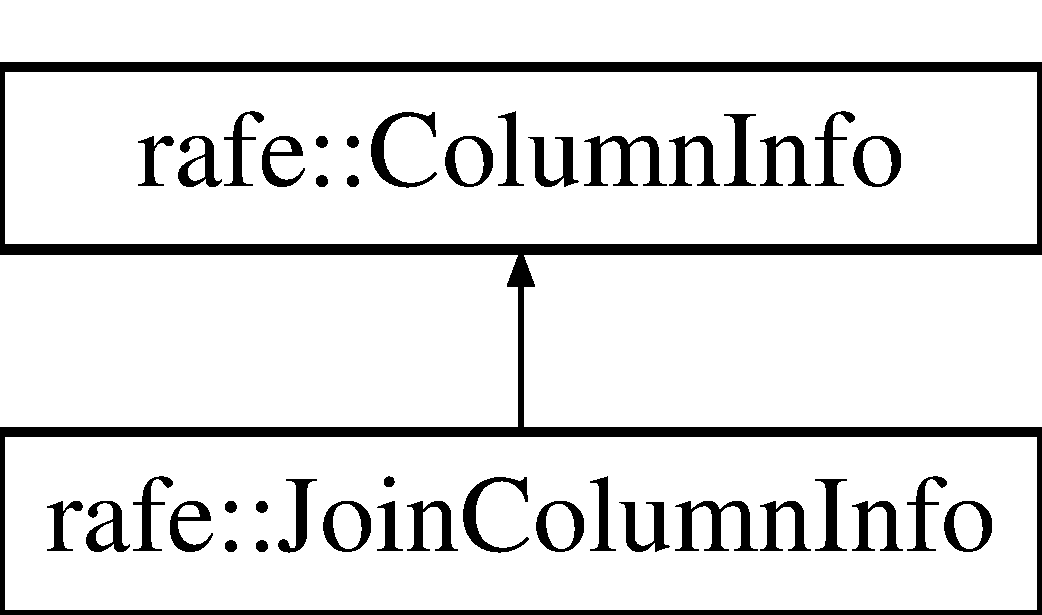
\includegraphics[height=2.000000cm]{classrafe_1_1_join_column_info}
\end{center}
\end{figure}
\subsection*{Public Member Functions}
\begin{DoxyCompactItemize}
\item 
\hyperlink{classrafe_1_1_join_column_info_ad9a1047f8f126fdbd6ad0530b852a8cf}{Join\+Column\+Info} (const \hyperlink{classrafe_1_1_column_info}{Column\+Info} \&col)
\item 
\hyperlink{classrafe_1_1_join_column_info_a2e4d6cec5ecfb6dfde9a91d3a9d05660}{Join\+Column\+Info} ()
\end{DoxyCompactItemize}
\subsection*{Public Attributes}
\begin{DoxyCompactItemize}
\item 
ulong \hyperlink{classrafe_1_1_join_column_info_af141ca99e62ec1ac85227b9da443a5f4}{input}
\item 
std\+::string \hyperlink{classrafe_1_1_join_column_info_af79ae87d9170139440abfac3fd89e199}{new\+Column}
\end{DoxyCompactItemize}


\subsection{Detailed Description}
Inherits from \hyperlink{classrafe_1_1_column_info}{Column\+Info} and stores additional information about optional column renaming. 

\subsection{Constructor \& Destructor Documentation}
\hypertarget{classrafe_1_1_join_column_info_ad9a1047f8f126fdbd6ad0530b852a8cf}{\index{rafe\+::\+Join\+Column\+Info@{rafe\+::\+Join\+Column\+Info}!Join\+Column\+Info@{Join\+Column\+Info}}
\index{Join\+Column\+Info@{Join\+Column\+Info}!rafe\+::\+Join\+Column\+Info@{rafe\+::\+Join\+Column\+Info}}
\subsubsection[{Join\+Column\+Info}]{\setlength{\rightskip}{0pt plus 5cm}rafe\+::\+Join\+Column\+Info\+::\+Join\+Column\+Info (
\begin{DoxyParamCaption}
\item[{const {\bf Column\+Info} \&}]{col}
\end{DoxyParamCaption}
)}}\label{classrafe_1_1_join_column_info_ad9a1047f8f126fdbd6ad0530b852a8cf}
Creates new instance of \hyperlink{classrafe_1_1_join_column_info}{Join\+Column\+Info}. 
\begin{DoxyParams}{Parameters}
{\em col} & -\/ \hyperlink{classrafe_1_1_column_info}{Column\+Info} \\
\hline
\end{DoxyParams}
\hypertarget{classrafe_1_1_join_column_info_a2e4d6cec5ecfb6dfde9a91d3a9d05660}{\index{rafe\+::\+Join\+Column\+Info@{rafe\+::\+Join\+Column\+Info}!Join\+Column\+Info@{Join\+Column\+Info}}
\index{Join\+Column\+Info@{Join\+Column\+Info}!rafe\+::\+Join\+Column\+Info@{rafe\+::\+Join\+Column\+Info}}
\subsubsection[{Join\+Column\+Info}]{\setlength{\rightskip}{0pt plus 5cm}rafe\+::\+Join\+Column\+Info\+::\+Join\+Column\+Info (
\begin{DoxyParamCaption}
{}
\end{DoxyParamCaption}
)}}\label{classrafe_1_1_join_column_info_a2e4d6cec5ecfb6dfde9a91d3a9d05660}
Creates new the instance of \hyperlink{classrafe_1_1_join_column_info}{Join\+Column\+Info}. 

\subsection{Member Data Documentation}
\hypertarget{classrafe_1_1_join_column_info_af141ca99e62ec1ac85227b9da443a5f4}{\index{rafe\+::\+Join\+Column\+Info@{rafe\+::\+Join\+Column\+Info}!input@{input}}
\index{input@{input}!rafe\+::\+Join\+Column\+Info@{rafe\+::\+Join\+Column\+Info}}
\subsubsection[{input}]{\setlength{\rightskip}{0pt plus 5cm}ulong rafe\+::\+Join\+Column\+Info\+::input}}\label{classrafe_1_1_join_column_info_af141ca99e62ec1ac85227b9da443a5f4}
Input, which column is from. Is is numbered from 0. \hypertarget{classrafe_1_1_join_column_info_af79ae87d9170139440abfac3fd89e199}{\index{rafe\+::\+Join\+Column\+Info@{rafe\+::\+Join\+Column\+Info}!new\+Column@{new\+Column}}
\index{new\+Column@{new\+Column}!rafe\+::\+Join\+Column\+Info@{rafe\+::\+Join\+Column\+Info}}
\subsubsection[{new\+Column}]{\setlength{\rightskip}{0pt plus 5cm}std\+::string rafe\+::\+Join\+Column\+Info\+::new\+Column}}\label{classrafe_1_1_join_column_info_af79ae87d9170139440abfac3fd89e199}
New column name. 

The documentation for this class was generated from the following files\+:\begin{DoxyCompactItemize}
\item 
C\+:/\+Users/\+Marcel/\+Documents/\+Visual Studio 2012/\+Projects/\+Relational\+Query\+Evaluator/\+Relational\+Query\+Evaluator/Algebra\+Structures.\+h\item 
C\+:/\+Users/\+Marcel/\+Documents/\+Visual Studio 2012/\+Projects/\+Relational\+Query\+Evaluator/\+Relational\+Query\+Evaluator/Algebra\+Structures.\+cpp\end{DoxyCompactItemize}

\hypertarget{classrafe_1_1_join_info}{\section{rafe\+:\+:Join\+Info Class Reference}
\label{classrafe_1_1_join_info}\index{rafe\+::\+Join\+Info@{rafe\+::\+Join\+Info}}
}


{\ttfamily \#include $<$Algebra\+Visitors.\+h$>$}

\subsection*{Public Member Functions}
\begin{DoxyCompactItemize}
\item 
void \hyperlink{classrafe_1_1_join_info_aef77063546aef0986b17dde67e89a581}{Remove\+Unnecessary\+Columns} (std\+::vector$<$ \hyperlink{classrafe_1_1_join_column_info}{Join\+Column\+Info} $>$ \&output\+Columns)
\end{DoxyCompactItemize}
\subsection*{Static Public Member Functions}
\begin{DoxyCompactItemize}
\item 
static bool \hyperlink{classrafe_1_1_join_info_aae492a171e8a72940722e35a30027e72}{Comparator} (const std\+::shared\+\_\+ptr$<$ \hyperlink{classrafe_1_1_join_info}{Join\+Info} $>$ \&lhs, const std\+::shared\+\_\+ptr$<$ \hyperlink{classrafe_1_1_join_info}{Join\+Info} $>$ \&rhs)
\end{DoxyCompactItemize}
\subsection*{Public Attributes}
\begin{DoxyCompactItemize}
\item 
std\+::vector$<$ std\+::shared\+\_\+ptr\\*
$<$ \hyperlink{classrafe_1_1_physical_plan}{Physical\+Plan} $>$ $>$ \hyperlink{classrafe_1_1_join_info_a1708cd5a22856820424f962b09066971}{plans}
\item 
std\+::set$<$ ulong $>$ \hyperlink{classrafe_1_1_join_info_aac96010c2f7c715f90e85e5ac25b31df}{processed\+Plans}
\item 
std\+::set$<$ ulong $>$ \hyperlink{classrafe_1_1_join_info_a430413badd7d9bd9c1d4bd27645ad98e}{un\+Processed\+Plans}
\item 
std\+::vector$<$ std\+::shared\+\_\+ptr\\*
$<$ \hyperlink{classrafe_1_1_condition_info}{Condition\+Info} $>$ $>$ \hyperlink{classrafe_1_1_join_info_a129f469fae807daf5195e930587050eb}{condition}
\item 
std\+::map$<$ int, \hyperlink{classrafe_1_1_join_column_info}{Join\+Column\+Info} $>$ \hyperlink{classrafe_1_1_join_info_a368a23397966ad965bf6de58d4471760}{columns}
\item 
double \hyperlink{classrafe_1_1_join_info_a3e362e7ce03809986b095b731119afc9}{size}
\end{DoxyCompactItemize}


\subsection{Detailed Description}
Structures storing information in join order algoritm. 

\subsection{Member Function Documentation}
\hypertarget{classrafe_1_1_join_info_aae492a171e8a72940722e35a30027e72}{\index{rafe\+::\+Join\+Info@{rafe\+::\+Join\+Info}!Comparator@{Comparator}}
\index{Comparator@{Comparator}!rafe\+::\+Join\+Info@{rafe\+::\+Join\+Info}}
\subsubsection[{Comparator}]{\setlength{\rightskip}{0pt plus 5cm}bool rafe\+::\+Join\+Info\+::\+Comparator (
\begin{DoxyParamCaption}
\item[{const std\+::shared\+\_\+ptr$<$ {\bf Join\+Info} $>$ \&}]{lhs, }
\item[{const std\+::shared\+\_\+ptr$<$ {\bf Join\+Info} $>$ \&}]{rhs}
\end{DoxyParamCaption}
)\hspace{0.3cm}{\ttfamily [static]}}}\label{classrafe_1_1_join_info_aae492a171e8a72940722e35a30027e72}
Comparer for head in greedy join order algorirthm. Compares plans bases on timecomplexity of plans\mbox{[}0\mbox{]}. Greedy join order algorirthm uses this structure with only one plan. 
\begin{DoxyParams}{Parameters}
{\em lhs} & -\/ first plan to compare. \\
\hline
{\em rhs} & -\/ second plan to compare. \\
\hline
\end{DoxyParams}
\begin{DoxyReturn}{Returns}
true if lsf is faster then rhs. 
\end{DoxyReturn}
\hypertarget{classrafe_1_1_join_info_aef77063546aef0986b17dde67e89a581}{\index{rafe\+::\+Join\+Info@{rafe\+::\+Join\+Info}!Remove\+Unnecessary\+Columns@{Remove\+Unnecessary\+Columns}}
\index{Remove\+Unnecessary\+Columns@{Remove\+Unnecessary\+Columns}!rafe\+::\+Join\+Info@{rafe\+::\+Join\+Info}}
\subsubsection[{Remove\+Unnecessary\+Columns}]{\setlength{\rightskip}{0pt plus 5cm}void rafe\+::\+Join\+Info\+::\+Remove\+Unnecessary\+Columns (
\begin{DoxyParamCaption}
\item[{std\+::vector$<$ {\bf Join\+Column\+Info} $>$ \&}]{output\+Columns}
\end{DoxyParamCaption}
)}}\label{classrafe_1_1_join_info_aef77063546aef0986b17dde67e89a581}
Remove unecessary columns from current plans. Unnecessary columns are the one, which are not in condition out in output of procesed Group\+Join. 
\begin{DoxyParams}{Parameters}
{\em output\+Columns} & columns which are necessary. \\
\hline
\end{DoxyParams}


\subsection{Member Data Documentation}
\hypertarget{classrafe_1_1_join_info_a368a23397966ad965bf6de58d4471760}{\index{rafe\+::\+Join\+Info@{rafe\+::\+Join\+Info}!columns@{columns}}
\index{columns@{columns}!rafe\+::\+Join\+Info@{rafe\+::\+Join\+Info}}
\subsubsection[{columns}]{\setlength{\rightskip}{0pt plus 5cm}std\+::map$<$int, {\bf Join\+Column\+Info}$>$ rafe\+::\+Join\+Info\+::columns}}\label{classrafe_1_1_join_info_a368a23397966ad965bf6de58d4471760}
Output columns from current plans. \hypertarget{classrafe_1_1_join_info_a129f469fae807daf5195e930587050eb}{\index{rafe\+::\+Join\+Info@{rafe\+::\+Join\+Info}!condition@{condition}}
\index{condition@{condition}!rafe\+::\+Join\+Info@{rafe\+::\+Join\+Info}}
\subsubsection[{condition}]{\setlength{\rightskip}{0pt plus 5cm}std\+::vector$<$std\+::shared\+\_\+ptr$<${\bf Condition\+Info}$>$ $>$ rafe\+::\+Join\+Info\+::condition}}\label{classrafe_1_1_join_info_a129f469fae807daf5195e930587050eb}
\hyperlink{classrafe_1_1_join}{Join} condition to be processed. \hypertarget{classrafe_1_1_join_info_a1708cd5a22856820424f962b09066971}{\index{rafe\+::\+Join\+Info@{rafe\+::\+Join\+Info}!plans@{plans}}
\index{plans@{plans}!rafe\+::\+Join\+Info@{rafe\+::\+Join\+Info}}
\subsubsection[{plans}]{\setlength{\rightskip}{0pt plus 5cm}std\+::vector$<$std\+::shared\+\_\+ptr$<${\bf Physical\+Plan}$>$ $>$ rafe\+::\+Join\+Info\+::plans}}\label{classrafe_1_1_join_info_a1708cd5a22856820424f962b09066971}
Generated plans. \hypertarget{classrafe_1_1_join_info_aac96010c2f7c715f90e85e5ac25b31df}{\index{rafe\+::\+Join\+Info@{rafe\+::\+Join\+Info}!processed\+Plans@{processed\+Plans}}
\index{processed\+Plans@{processed\+Plans}!rafe\+::\+Join\+Info@{rafe\+::\+Join\+Info}}
\subsubsection[{processed\+Plans}]{\setlength{\rightskip}{0pt plus 5cm}std\+::set$<$ulong$>$ rafe\+::\+Join\+Info\+::processed\+Plans}}\label{classrafe_1_1_join_info_aac96010c2f7c715f90e85e5ac25b31df}
Numbers of processed inputs. \hypertarget{classrafe_1_1_join_info_a3e362e7ce03809986b095b731119afc9}{\index{rafe\+::\+Join\+Info@{rafe\+::\+Join\+Info}!size@{size}}
\index{size@{size}!rafe\+::\+Join\+Info@{rafe\+::\+Join\+Info}}
\subsubsection[{size}]{\setlength{\rightskip}{0pt plus 5cm}double rafe\+::\+Join\+Info\+::size}}\label{classrafe_1_1_join_info_a3e362e7ce03809986b095b731119afc9}
Size of the processed relation. \hypertarget{classrafe_1_1_join_info_a430413badd7d9bd9c1d4bd27645ad98e}{\index{rafe\+::\+Join\+Info@{rafe\+::\+Join\+Info}!un\+Processed\+Plans@{un\+Processed\+Plans}}
\index{un\+Processed\+Plans@{un\+Processed\+Plans}!rafe\+::\+Join\+Info@{rafe\+::\+Join\+Info}}
\subsubsection[{un\+Processed\+Plans}]{\setlength{\rightskip}{0pt plus 5cm}std\+::set$<$ulong$>$ rafe\+::\+Join\+Info\+::un\+Processed\+Plans}}\label{classrafe_1_1_join_info_a430413badd7d9bd9c1d4bd27645ad98e}
Numbers of unprocessed inputs. 

The documentation for this class was generated from the following files\+:\begin{DoxyCompactItemize}
\item 
C\+:/\+Users/\+Marcel/\+Documents/\+Visual Studio 2012/\+Projects/\+Relational\+Query\+Evaluator/\+Relational\+Query\+Evaluator/Algebra\+Visitors.\+h\item 
C\+:/\+Users/\+Marcel/\+Documents/\+Visual Studio 2012/\+Projects/\+Relational\+Query\+Evaluator/\+Relational\+Query\+Evaluator/Algebra\+Compiler.\+cpp\end{DoxyCompactItemize}

\hypertarget{classrafe_1_1_join_info_reading_expression_visitor}{\section{rafe\+:\+:Join\+Info\+Reading\+Expression\+Visitor Class Reference}
\label{classrafe_1_1_join_info_reading_expression_visitor}\index{rafe\+::\+Join\+Info\+Reading\+Expression\+Visitor@{rafe\+::\+Join\+Info\+Reading\+Expression\+Visitor}}
}


{\ttfamily \#include $<$Expression\+Visitors.\+h$>$}

Inheritance diagram for rafe\+:\+:Join\+Info\+Reading\+Expression\+Visitor\+:\begin{figure}[H]
\begin{center}
\leavevmode
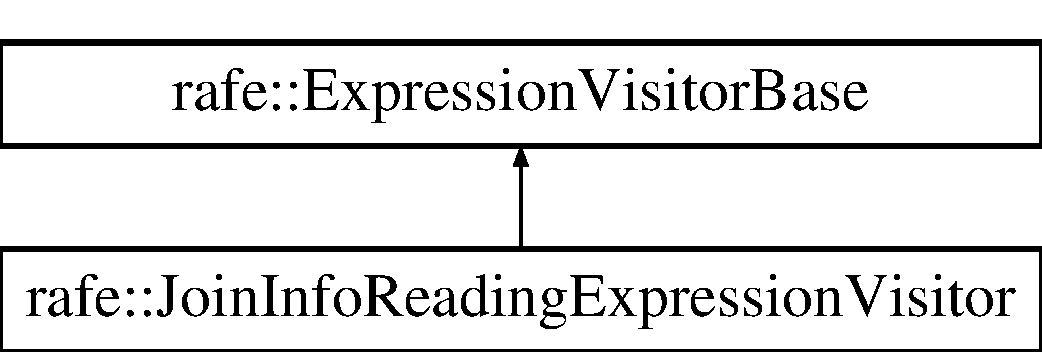
\includegraphics[height=2.000000cm]{classrafe_1_1_join_info_reading_expression_visitor}
\end{center}
\end{figure}
\subsection*{Public Member Functions}
\begin{DoxyCompactItemize}
\item 
\hyperlink{classrafe_1_1_join_info_reading_expression_visitor_a964f1d36e020a9099314400c1b400754}{Join\+Info\+Reading\+Expression\+Visitor} (std\+::set$<$ int $>$ $\ast$\hyperlink{classrafe_1_1_join_info_reading_expression_visitor_a9e734526bd1f92d980024ce0dbed65ba}{data}, Condition\+Type $\ast$type)
\item 
void \hyperlink{classrafe_1_1_join_info_reading_expression_visitor_a791b1f98544255f24c39b77286b459d9}{visit\+Column} (\hyperlink{classrafe_1_1_column}{Column} $\ast$expression)
\item 
void \hyperlink{classrafe_1_1_join_info_reading_expression_visitor_a27ebab51d1b63683004f2ec45d15869f}{visit\+Unary\+Expression} (\hyperlink{classrafe_1_1_unary_expression}{Unary\+Expression} $\ast$expression)
\item 
void \hyperlink{classrafe_1_1_join_info_reading_expression_visitor_a3fe9a23de3b525cc967c0f8b1c2c81eb}{visit\+Binary\+Expression} (\hyperlink{classrafe_1_1_binary_expression}{Binary\+Expression} $\ast$expression)
\item 
void \hyperlink{classrafe_1_1_join_info_reading_expression_visitor_a57a8dedf4fa06ff27c71cf36ee7a4b3b}{visit\+Nnary\+Expression} (\hyperlink{classrafe_1_1_nnary_expression}{Nnary\+Expression} $\ast$expression)
\item 
void \hyperlink{classrafe_1_1_join_info_reading_expression_visitor_aa08dee45829be99a6c6b3961c8cf081d}{visit\+Constant} (\hyperlink{classrafe_1_1_constant}{Constant} $\ast$expression)
\item 
void \hyperlink{classrafe_1_1_join_info_reading_expression_visitor_acfd9c7c62dfac50b0ac6d1c314f7f395}{visit\+Grouped\+Expression} (\hyperlink{classrafe_1_1_grouped_expression}{Grouped\+Expression} $\ast$expression)
\end{DoxyCompactItemize}
\subsection*{Public Attributes}
\begin{DoxyCompactItemize}
\item 
std\+::set$<$ int $>$ $\ast$ \hyperlink{classrafe_1_1_join_info_reading_expression_visitor_a9e734526bd1f92d980024ce0dbed65ba}{data}
\item 
Condition\+Type $\ast$ \hyperlink{classrafe_1_1_join_info_reading_expression_visitor_a76585d743cb5babfeca7bd239bc01fca}{condition\+Type}
\end{DoxyCompactItemize}


\subsection{Detailed Description}
Reads all columns identifiers from expression and determing what kind of condition is expression representing. It can be equal condition a=b or condition a1$<$b$<$a2. Other conditions should not be in joins. 

\subsection{Constructor \& Destructor Documentation}
\hypertarget{classrafe_1_1_join_info_reading_expression_visitor_a964f1d36e020a9099314400c1b400754}{\index{rafe\+::\+Join\+Info\+Reading\+Expression\+Visitor@{rafe\+::\+Join\+Info\+Reading\+Expression\+Visitor}!Join\+Info\+Reading\+Expression\+Visitor@{Join\+Info\+Reading\+Expression\+Visitor}}
\index{Join\+Info\+Reading\+Expression\+Visitor@{Join\+Info\+Reading\+Expression\+Visitor}!rafe\+::\+Join\+Info\+Reading\+Expression\+Visitor@{rafe\+::\+Join\+Info\+Reading\+Expression\+Visitor}}
\subsubsection[{Join\+Info\+Reading\+Expression\+Visitor}]{\setlength{\rightskip}{0pt plus 5cm}rafe\+::\+Join\+Info\+Reading\+Expression\+Visitor\+::\+Join\+Info\+Reading\+Expression\+Visitor (
\begin{DoxyParamCaption}
\item[{std\+::set$<$ int $>$ $\ast$}]{data, }
\item[{Condition\+Type $\ast$}]{type}
\end{DoxyParamCaption}
)}}\label{classrafe_1_1_join_info_reading_expression_visitor_a964f1d36e020a9099314400c1b400754}
Creates new instance of \hyperlink{classrafe_1_1_join_info_reading_expression_visitor}{Join\+Info\+Reading\+Expression\+Visitor}. 
\begin{DoxyParams}{Parameters}
{\em data} & -\/ visitor will store here unique column identifiers. \\
\hline
{\em type} & -\/ visitor will store here condition type. \\
\hline
\end{DoxyParams}


\subsection{Member Function Documentation}
\hypertarget{classrafe_1_1_join_info_reading_expression_visitor_a3fe9a23de3b525cc967c0f8b1c2c81eb}{\index{rafe\+::\+Join\+Info\+Reading\+Expression\+Visitor@{rafe\+::\+Join\+Info\+Reading\+Expression\+Visitor}!visit\+Binary\+Expression@{visit\+Binary\+Expression}}
\index{visit\+Binary\+Expression@{visit\+Binary\+Expression}!rafe\+::\+Join\+Info\+Reading\+Expression\+Visitor@{rafe\+::\+Join\+Info\+Reading\+Expression\+Visitor}}
\subsubsection[{visit\+Binary\+Expression}]{\setlength{\rightskip}{0pt plus 5cm}void rafe\+::\+Join\+Info\+Reading\+Expression\+Visitor\+::visit\+Binary\+Expression (
\begin{DoxyParamCaption}
\item[{{\bf Binary\+Expression} $\ast$}]{expression}
\end{DoxyParamCaption}
)\hspace{0.3cm}{\ttfamily [virtual]}}}\label{classrafe_1_1_join_info_reading_expression_visitor_a3fe9a23de3b525cc967c0f8b1c2c81eb}
Visits \hyperlink{classrafe_1_1_binary_expression}{Binary\+Expression} node. 
\begin{DoxyParams}{Parameters}
{\em expression} & visited \hyperlink{classrafe_1_1_binary_expression}{Binary\+Expression}. \\
\hline
\end{DoxyParams}


Reimplemented from \hyperlink{classrafe_1_1_expression_visitor_base_a63e53276af3a22d3592f34d05ba97014}{rafe\+::\+Expression\+Visitor\+Base}.

\hypertarget{classrafe_1_1_join_info_reading_expression_visitor_a791b1f98544255f24c39b77286b459d9}{\index{rafe\+::\+Join\+Info\+Reading\+Expression\+Visitor@{rafe\+::\+Join\+Info\+Reading\+Expression\+Visitor}!visit\+Column@{visit\+Column}}
\index{visit\+Column@{visit\+Column}!rafe\+::\+Join\+Info\+Reading\+Expression\+Visitor@{rafe\+::\+Join\+Info\+Reading\+Expression\+Visitor}}
\subsubsection[{visit\+Column}]{\setlength{\rightskip}{0pt plus 5cm}void rafe\+::\+Join\+Info\+Reading\+Expression\+Visitor\+::visit\+Column (
\begin{DoxyParamCaption}
\item[{{\bf Column} $\ast$}]{expression}
\end{DoxyParamCaption}
)\hspace{0.3cm}{\ttfamily [virtual]}}}\label{classrafe_1_1_join_info_reading_expression_visitor_a791b1f98544255f24c39b77286b459d9}
Visits \hyperlink{classrafe_1_1_column}{Column} node. 
\begin{DoxyParams}{Parameters}
{\em expression} & visited \hyperlink{classrafe_1_1_column}{Column}. \\
\hline
\end{DoxyParams}


Reimplemented from \hyperlink{classrafe_1_1_expression_visitor_base_a4eaa77bf4105d1cbdde4feb047228255}{rafe\+::\+Expression\+Visitor\+Base}.

\hypertarget{classrafe_1_1_join_info_reading_expression_visitor_aa08dee45829be99a6c6b3961c8cf081d}{\index{rafe\+::\+Join\+Info\+Reading\+Expression\+Visitor@{rafe\+::\+Join\+Info\+Reading\+Expression\+Visitor}!visit\+Constant@{visit\+Constant}}
\index{visit\+Constant@{visit\+Constant}!rafe\+::\+Join\+Info\+Reading\+Expression\+Visitor@{rafe\+::\+Join\+Info\+Reading\+Expression\+Visitor}}
\subsubsection[{visit\+Constant}]{\setlength{\rightskip}{0pt plus 5cm}void rafe\+::\+Join\+Info\+Reading\+Expression\+Visitor\+::visit\+Constant (
\begin{DoxyParamCaption}
\item[{{\bf Constant} $\ast$}]{expression}
\end{DoxyParamCaption}
)\hspace{0.3cm}{\ttfamily [virtual]}}}\label{classrafe_1_1_join_info_reading_expression_visitor_aa08dee45829be99a6c6b3961c8cf081d}
Visits \hyperlink{classrafe_1_1_constant}{Constant} node. 
\begin{DoxyParams}{Parameters}
{\em expression} & visited \hyperlink{classrafe_1_1_constant}{Constant}. \\
\hline
\end{DoxyParams}


Reimplemented from \hyperlink{classrafe_1_1_expression_visitor_base_af934111c6881f9f6c3ef3aa51425b9ff}{rafe\+::\+Expression\+Visitor\+Base}.

\hypertarget{classrafe_1_1_join_info_reading_expression_visitor_acfd9c7c62dfac50b0ac6d1c314f7f395}{\index{rafe\+::\+Join\+Info\+Reading\+Expression\+Visitor@{rafe\+::\+Join\+Info\+Reading\+Expression\+Visitor}!visit\+Grouped\+Expression@{visit\+Grouped\+Expression}}
\index{visit\+Grouped\+Expression@{visit\+Grouped\+Expression}!rafe\+::\+Join\+Info\+Reading\+Expression\+Visitor@{rafe\+::\+Join\+Info\+Reading\+Expression\+Visitor}}
\subsubsection[{visit\+Grouped\+Expression}]{\setlength{\rightskip}{0pt plus 5cm}void rafe\+::\+Join\+Info\+Reading\+Expression\+Visitor\+::visit\+Grouped\+Expression (
\begin{DoxyParamCaption}
\item[{{\bf Grouped\+Expression} $\ast$}]{expression}
\end{DoxyParamCaption}
)\hspace{0.3cm}{\ttfamily [virtual]}}}\label{classrafe_1_1_join_info_reading_expression_visitor_acfd9c7c62dfac50b0ac6d1c314f7f395}
Visits \hyperlink{classrafe_1_1_grouped_expression}{Grouped\+Expression} node. 
\begin{DoxyParams}{Parameters}
{\em expression} & visited \hyperlink{classrafe_1_1_grouped_expression}{Grouped\+Expression}. \\
\hline
\end{DoxyParams}


Reimplemented from \hyperlink{classrafe_1_1_expression_visitor_base_a76226ab9d571ed7eaf80d2ed7153791c}{rafe\+::\+Expression\+Visitor\+Base}.

\hypertarget{classrafe_1_1_join_info_reading_expression_visitor_a57a8dedf4fa06ff27c71cf36ee7a4b3b}{\index{rafe\+::\+Join\+Info\+Reading\+Expression\+Visitor@{rafe\+::\+Join\+Info\+Reading\+Expression\+Visitor}!visit\+Nnary\+Expression@{visit\+Nnary\+Expression}}
\index{visit\+Nnary\+Expression@{visit\+Nnary\+Expression}!rafe\+::\+Join\+Info\+Reading\+Expression\+Visitor@{rafe\+::\+Join\+Info\+Reading\+Expression\+Visitor}}
\subsubsection[{visit\+Nnary\+Expression}]{\setlength{\rightskip}{0pt plus 5cm}void rafe\+::\+Join\+Info\+Reading\+Expression\+Visitor\+::visit\+Nnary\+Expression (
\begin{DoxyParamCaption}
\item[{{\bf Nnary\+Expression} $\ast$}]{expression}
\end{DoxyParamCaption}
)\hspace{0.3cm}{\ttfamily [virtual]}}}\label{classrafe_1_1_join_info_reading_expression_visitor_a57a8dedf4fa06ff27c71cf36ee7a4b3b}
Visits \hyperlink{classrafe_1_1_nnary_expression}{Nnary\+Expression} node. 
\begin{DoxyParams}{Parameters}
{\em expression} & visited \hyperlink{classrafe_1_1_nnary_expression}{Nnary\+Expression}. \\
\hline
\end{DoxyParams}


Reimplemented from \hyperlink{classrafe_1_1_expression_visitor_base_a32f89977f780ccb8aabe5afa1fa42d45}{rafe\+::\+Expression\+Visitor\+Base}.

\hypertarget{classrafe_1_1_join_info_reading_expression_visitor_a27ebab51d1b63683004f2ec45d15869f}{\index{rafe\+::\+Join\+Info\+Reading\+Expression\+Visitor@{rafe\+::\+Join\+Info\+Reading\+Expression\+Visitor}!visit\+Unary\+Expression@{visit\+Unary\+Expression}}
\index{visit\+Unary\+Expression@{visit\+Unary\+Expression}!rafe\+::\+Join\+Info\+Reading\+Expression\+Visitor@{rafe\+::\+Join\+Info\+Reading\+Expression\+Visitor}}
\subsubsection[{visit\+Unary\+Expression}]{\setlength{\rightskip}{0pt plus 5cm}void rafe\+::\+Join\+Info\+Reading\+Expression\+Visitor\+::visit\+Unary\+Expression (
\begin{DoxyParamCaption}
\item[{{\bf Unary\+Expression} $\ast$}]{expression}
\end{DoxyParamCaption}
)\hspace{0.3cm}{\ttfamily [virtual]}}}\label{classrafe_1_1_join_info_reading_expression_visitor_a27ebab51d1b63683004f2ec45d15869f}
Visits \hyperlink{classrafe_1_1_unary_expression}{Unary\+Expression} node. 
\begin{DoxyParams}{Parameters}
{\em expression} & visited \hyperlink{classrafe_1_1_unary_expression}{Unary\+Expression}. \\
\hline
\end{DoxyParams}


Reimplemented from \hyperlink{classrafe_1_1_expression_visitor_base_a439348ee979dff26c30707f1ef499e8c}{rafe\+::\+Expression\+Visitor\+Base}.



\subsection{Member Data Documentation}
\hypertarget{classrafe_1_1_join_info_reading_expression_visitor_a76585d743cb5babfeca7bd239bc01fca}{\index{rafe\+::\+Join\+Info\+Reading\+Expression\+Visitor@{rafe\+::\+Join\+Info\+Reading\+Expression\+Visitor}!condition\+Type@{condition\+Type}}
\index{condition\+Type@{condition\+Type}!rafe\+::\+Join\+Info\+Reading\+Expression\+Visitor@{rafe\+::\+Join\+Info\+Reading\+Expression\+Visitor}}
\subsubsection[{condition\+Type}]{\setlength{\rightskip}{0pt plus 5cm}Condition\+Type$\ast$ rafe\+::\+Join\+Info\+Reading\+Expression\+Visitor\+::condition\+Type}}\label{classrafe_1_1_join_info_reading_expression_visitor_a76585d743cb5babfeca7bd239bc01fca}
Type of join condition. \hypertarget{classrafe_1_1_join_info_reading_expression_visitor_a9e734526bd1f92d980024ce0dbed65ba}{\index{rafe\+::\+Join\+Info\+Reading\+Expression\+Visitor@{rafe\+::\+Join\+Info\+Reading\+Expression\+Visitor}!data@{data}}
\index{data@{data}!rafe\+::\+Join\+Info\+Reading\+Expression\+Visitor@{rafe\+::\+Join\+Info\+Reading\+Expression\+Visitor}}
\subsubsection[{data}]{\setlength{\rightskip}{0pt plus 5cm}std\+::set$<$int$>$$\ast$ rafe\+::\+Join\+Info\+Reading\+Expression\+Visitor\+::data}}\label{classrafe_1_1_join_info_reading_expression_visitor_a9e734526bd1f92d980024ce0dbed65ba}
Set of unique columns identifiers. 

The documentation for this class was generated from the following files\+:\begin{DoxyCompactItemize}
\item 
C\+:/\+Users/\+Marcel/\+Documents/\+Visual Studio 2012/\+Projects/\+Relational\+Query\+Evaluator/\+Relational\+Query\+Evaluator/Expression\+Visitors.\+h\item 
C\+:/\+Users/\+Marcel/\+Documents/\+Visual Studio 2012/\+Projects/\+Relational\+Query\+Evaluator/\+Relational\+Query\+Evaluator/Expression\+Visitors.\+cpp\end{DoxyCompactItemize}

\hypertarget{classrafe_1_1_max_of_unique_values_expression_visitor}{\section{rafe\+:\+:Max\+Of\+Unique\+Values\+Expression\+Visitor Class Reference}
\label{classrafe_1_1_max_of_unique_values_expression_visitor}\index{rafe\+::\+Max\+Of\+Unique\+Values\+Expression\+Visitor@{rafe\+::\+Max\+Of\+Unique\+Values\+Expression\+Visitor}}
}


{\ttfamily \#include $<$Expression\+Visitors.\+h$>$}

Inheritance diagram for rafe\+:\+:Max\+Of\+Unique\+Values\+Expression\+Visitor\+:\begin{figure}[H]
\begin{center}
\leavevmode
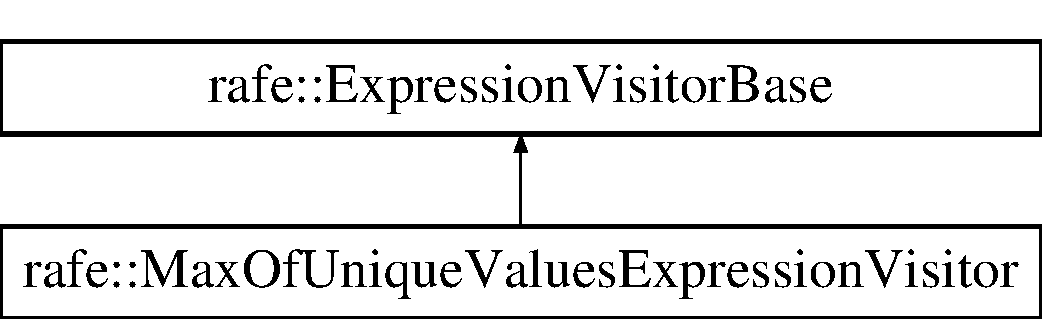
\includegraphics[height=2.000000cm]{classrafe_1_1_max_of_unique_values_expression_visitor}
\end{center}
\end{figure}
\subsection*{Public Member Functions}
\begin{DoxyCompactItemize}
\item 
\hyperlink{classrafe_1_1_max_of_unique_values_expression_visitor_ab14921bdb9f894add695d68b23152c09}{Max\+Of\+Unique\+Values\+Expression\+Visitor} (std\+::map$<$ int, \hyperlink{classrafe_1_1_column_info}{Column\+Info} $>$ $\ast$cols)
\item 
void \hyperlink{classrafe_1_1_max_of_unique_values_expression_visitor_af7018ac8dc1f162aa263d16e0c9f757a}{visit\+Column} (\hyperlink{classrafe_1_1_column}{Column} $\ast$expression)
\end{DoxyCompactItemize}
\subsection*{Public Attributes}
\begin{DoxyCompactItemize}
\item 
double \hyperlink{classrafe_1_1_max_of_unique_values_expression_visitor_a759f44c4d4b051aec0f057bead093f77}{result}
\item 
std\+::map$<$ int, \hyperlink{classrafe_1_1_column_info}{Column\+Info} $>$ $\ast$ \hyperlink{classrafe_1_1_max_of_unique_values_expression_visitor_a11f28e944ba731456477cc8ec13c73e5}{columns}
\end{DoxyCompactItemize}


\subsection{Detailed Description}
Visitor is used in join calculation to estimate size of relation after join. It computes maximum of unique values in each colum and stores the result in result variable. 

\subsection{Constructor \& Destructor Documentation}
\hypertarget{classrafe_1_1_max_of_unique_values_expression_visitor_ab14921bdb9f894add695d68b23152c09}{\index{rafe\+::\+Max\+Of\+Unique\+Values\+Expression\+Visitor@{rafe\+::\+Max\+Of\+Unique\+Values\+Expression\+Visitor}!Max\+Of\+Unique\+Values\+Expression\+Visitor@{Max\+Of\+Unique\+Values\+Expression\+Visitor}}
\index{Max\+Of\+Unique\+Values\+Expression\+Visitor@{Max\+Of\+Unique\+Values\+Expression\+Visitor}!rafe\+::\+Max\+Of\+Unique\+Values\+Expression\+Visitor@{rafe\+::\+Max\+Of\+Unique\+Values\+Expression\+Visitor}}
\subsubsection[{Max\+Of\+Unique\+Values\+Expression\+Visitor}]{\setlength{\rightskip}{0pt plus 5cm}rafe\+::\+Max\+Of\+Unique\+Values\+Expression\+Visitor\+::\+Max\+Of\+Unique\+Values\+Expression\+Visitor (
\begin{DoxyParamCaption}
\item[{std\+::map$<$ int, {\bf Column\+Info} $>$ $\ast$}]{cols}
\end{DoxyParamCaption}
)}}\label{classrafe_1_1_max_of_unique_values_expression_visitor_ab14921bdb9f894add695d68b23152c09}
Creates new instance of \hyperlink{classrafe_1_1_max_of_unique_values_expression_visitor}{Max\+Of\+Unique\+Values\+Expression\+Visitor}. 
\begin{DoxyParams}{Parameters}
{\em cols} & -\/ structure mapping column unique identifier to number of column in processed bobox operator \\
\hline
\end{DoxyParams}


\subsection{Member Function Documentation}
\hypertarget{classrafe_1_1_max_of_unique_values_expression_visitor_af7018ac8dc1f162aa263d16e0c9f757a}{\index{rafe\+::\+Max\+Of\+Unique\+Values\+Expression\+Visitor@{rafe\+::\+Max\+Of\+Unique\+Values\+Expression\+Visitor}!visit\+Column@{visit\+Column}}
\index{visit\+Column@{visit\+Column}!rafe\+::\+Max\+Of\+Unique\+Values\+Expression\+Visitor@{rafe\+::\+Max\+Of\+Unique\+Values\+Expression\+Visitor}}
\subsubsection[{visit\+Column}]{\setlength{\rightskip}{0pt plus 5cm}void rafe\+::\+Max\+Of\+Unique\+Values\+Expression\+Visitor\+::visit\+Column (
\begin{DoxyParamCaption}
\item[{{\bf Column} $\ast$}]{expression}
\end{DoxyParamCaption}
)\hspace{0.3cm}{\ttfamily [virtual]}}}\label{classrafe_1_1_max_of_unique_values_expression_visitor_af7018ac8dc1f162aa263d16e0c9f757a}
Visits \hyperlink{classrafe_1_1_column}{Column} node. 
\begin{DoxyParams}{Parameters}
{\em expression} & visited \hyperlink{classrafe_1_1_column}{Column}. \\
\hline
\end{DoxyParams}


Reimplemented from \hyperlink{classrafe_1_1_expression_visitor_base_a4eaa77bf4105d1cbdde4feb047228255}{rafe\+::\+Expression\+Visitor\+Base}.



\subsection{Member Data Documentation}
\hypertarget{classrafe_1_1_max_of_unique_values_expression_visitor_a11f28e944ba731456477cc8ec13c73e5}{\index{rafe\+::\+Max\+Of\+Unique\+Values\+Expression\+Visitor@{rafe\+::\+Max\+Of\+Unique\+Values\+Expression\+Visitor}!columns@{columns}}
\index{columns@{columns}!rafe\+::\+Max\+Of\+Unique\+Values\+Expression\+Visitor@{rafe\+::\+Max\+Of\+Unique\+Values\+Expression\+Visitor}}
\subsubsection[{columns}]{\setlength{\rightskip}{0pt plus 5cm}std\+::map$<$int, {\bf Column\+Info}$>$$\ast$ rafe\+::\+Max\+Of\+Unique\+Values\+Expression\+Visitor\+::columns}}\label{classrafe_1_1_max_of_unique_values_expression_visitor_a11f28e944ba731456477cc8ec13c73e5}
Map of columns in this expression. Key is unique column identifier. \hypertarget{classrafe_1_1_max_of_unique_values_expression_visitor_a759f44c4d4b051aec0f057bead093f77}{\index{rafe\+::\+Max\+Of\+Unique\+Values\+Expression\+Visitor@{rafe\+::\+Max\+Of\+Unique\+Values\+Expression\+Visitor}!result@{result}}
\index{result@{result}!rafe\+::\+Max\+Of\+Unique\+Values\+Expression\+Visitor@{rafe\+::\+Max\+Of\+Unique\+Values\+Expression\+Visitor}}
\subsubsection[{result}]{\setlength{\rightskip}{0pt plus 5cm}double rafe\+::\+Max\+Of\+Unique\+Values\+Expression\+Visitor\+::result}}\label{classrafe_1_1_max_of_unique_values_expression_visitor_a759f44c4d4b051aec0f057bead093f77}
Visitor stores here maximum of unique values of all columns in visited expression. 

The documentation for this class was generated from the following files\+:\begin{DoxyCompactItemize}
\item 
C\+:/\+Users/\+Marcel/\+Documents/\+Visual Studio 2012/\+Projects/\+Relational\+Query\+Evaluator/\+Relational\+Query\+Evaluator/Expression\+Visitors.\+h\item 
C\+:/\+Users/\+Marcel/\+Documents/\+Visual Studio 2012/\+Projects/\+Relational\+Query\+Evaluator/\+Relational\+Query\+Evaluator/Expression\+Visitors.\+cpp\end{DoxyCompactItemize}

\hypertarget{classrafe_1_1_merge_anti_join}{\section{rafe\+:\+:Merge\+Anti\+Join Class Reference}
\label{classrafe_1_1_merge_anti_join}\index{rafe\+::\+Merge\+Anti\+Join@{rafe\+::\+Merge\+Anti\+Join}}
}


{\ttfamily \#include $<$Physical\+Operator.\+h$>$}

Inheritance diagram for rafe\+:\+:Merge\+Anti\+Join\+:\begin{figure}[H]
\begin{center}
\leavevmode
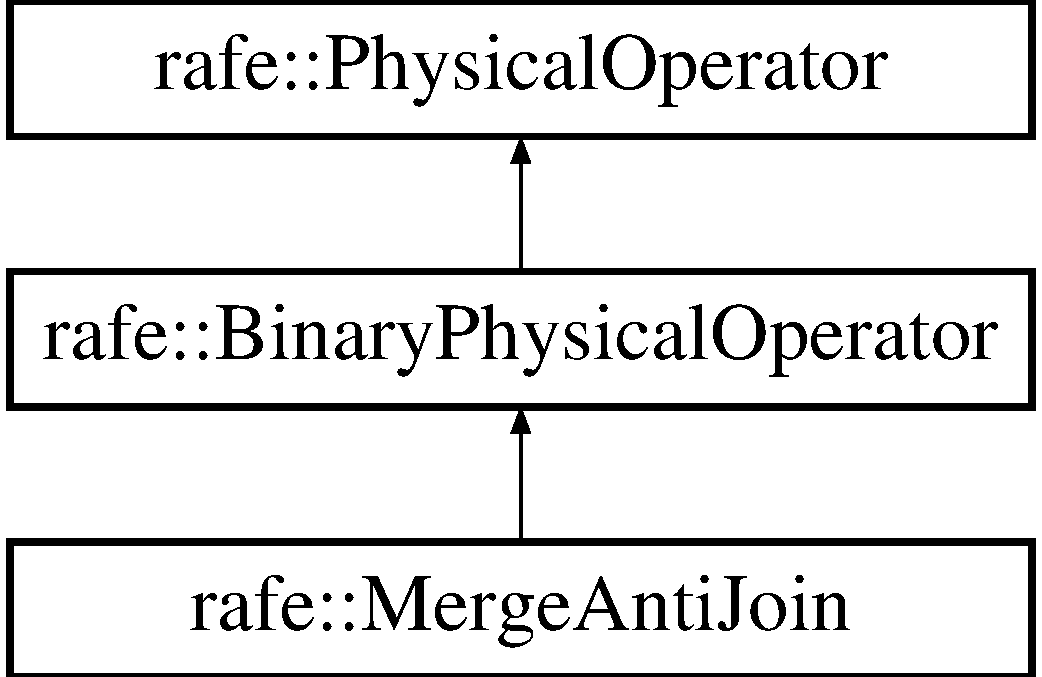
\includegraphics[height=3.000000cm]{classrafe_1_1_merge_anti_join}
\end{center}
\end{figure}
\subsection*{Public Member Functions}
\begin{DoxyCompactItemize}
\item 
\hyperlink{classrafe_1_1_merge_anti_join_ad67fe6bf33d22aa9e86cc7b022509adf}{Merge\+Anti\+Join} (const std\+::shared\+\_\+ptr$<$ \hyperlink{classrafe_1_1_expression}{Expression} $>$ \&\hyperlink{classrafe_1_1_merge_anti_join_a25262bcb30b68e719e540c6237f56228}{condition})
\item 
void \hyperlink{classrafe_1_1_merge_anti_join_aae93ebacaaed68ab8af8f38a09cfe8e7}{accept} (\hyperlink{classrafe_1_1_physical_operator_visitor}{Physical\+Operator\+Visitor} \&v)
\end{DoxyCompactItemize}
\subsection*{Public Attributes}
\begin{DoxyCompactItemize}
\item 
std\+::shared\+\_\+ptr$<$ \hyperlink{classrafe_1_1_expression}{Expression} $>$ \hyperlink{classrafe_1_1_merge_anti_join_a25262bcb30b68e719e540c6237f56228}{condition}
\item 
std\+::vector$<$ \hyperlink{classrafe_1_1_sort_parameter}{Sort\+Parameter} $>$ \hyperlink{classrafe_1_1_merge_anti_join_adde369c7d6dcdeb5530b40999af4c4c4}{left}
\item 
std\+::vector$<$ \hyperlink{classrafe_1_1_sort_parameter}{Sort\+Parameter} $>$ \hyperlink{classrafe_1_1_merge_anti_join_a278393533a0b0a6f3c38ba6810abf221}{right}
\end{DoxyCompactItemize}


\subsection{Detailed Description}
Represents Merge equi anti join. Operator computes equi anti join from given sorted inputs. 

\subsection{Constructor \& Destructor Documentation}
\hypertarget{classrafe_1_1_merge_anti_join_ad67fe6bf33d22aa9e86cc7b022509adf}{\index{rafe\+::\+Merge\+Anti\+Join@{rafe\+::\+Merge\+Anti\+Join}!Merge\+Anti\+Join@{Merge\+Anti\+Join}}
\index{Merge\+Anti\+Join@{Merge\+Anti\+Join}!rafe\+::\+Merge\+Anti\+Join@{rafe\+::\+Merge\+Anti\+Join}}
\subsubsection[{Merge\+Anti\+Join}]{\setlength{\rightskip}{0pt plus 5cm}rafe\+::\+Merge\+Anti\+Join\+::\+Merge\+Anti\+Join (
\begin{DoxyParamCaption}
\item[{const std\+::shared\+\_\+ptr$<$ {\bf Expression} $>$ \&}]{condition}
\end{DoxyParamCaption}
)}}\label{classrafe_1_1_merge_anti_join_ad67fe6bf33d22aa9e86cc7b022509adf}
Creates new instance of \hyperlink{classrafe_1_1_merge_anti_join}{Merge\+Anti\+Join}. 
\begin{DoxyParams}{Parameters}
{\em condition} & -\/ join condition. \\
\hline
\end{DoxyParams}


\subsection{Member Function Documentation}
\hypertarget{classrafe_1_1_merge_anti_join_aae93ebacaaed68ab8af8f38a09cfe8e7}{\index{rafe\+::\+Merge\+Anti\+Join@{rafe\+::\+Merge\+Anti\+Join}!accept@{accept}}
\index{accept@{accept}!rafe\+::\+Merge\+Anti\+Join@{rafe\+::\+Merge\+Anti\+Join}}
\subsubsection[{accept}]{\setlength{\rightskip}{0pt plus 5cm}void rafe\+::\+Merge\+Anti\+Join\+::accept (
\begin{DoxyParamCaption}
\item[{{\bf Physical\+Operator\+Visitor} \&}]{v}
\end{DoxyParamCaption}
)\hspace{0.3cm}{\ttfamily [virtual]}}}\label{classrafe_1_1_merge_anti_join_aae93ebacaaed68ab8af8f38a09cfe8e7}
Method for calling visit\mbox{[}node\mbox{]} on given \hyperlink{classrafe_1_1_physical_operator_visitor}{Physical\+Operator\+Visitor}. 
\begin{DoxyParams}{Parameters}
{\em v} & \hyperlink{classrafe_1_1_physical_operator_visitor}{Physical\+Operator\+Visitor}, on which to call function. \\
\hline
\end{DoxyParams}


Implements \hyperlink{classrafe_1_1_binary_physical_operator_a58ce0a14b970b2c932254419877a2e0e}{rafe\+::\+Binary\+Physical\+Operator}.



\subsection{Member Data Documentation}
\hypertarget{classrafe_1_1_merge_anti_join_a25262bcb30b68e719e540c6237f56228}{\index{rafe\+::\+Merge\+Anti\+Join@{rafe\+::\+Merge\+Anti\+Join}!condition@{condition}}
\index{condition@{condition}!rafe\+::\+Merge\+Anti\+Join@{rafe\+::\+Merge\+Anti\+Join}}
\subsubsection[{condition}]{\setlength{\rightskip}{0pt plus 5cm}std\+::shared\+\_\+ptr$<${\bf Expression}$>$ rafe\+::\+Merge\+Anti\+Join\+::condition}}\label{classrafe_1_1_merge_anti_join_a25262bcb30b68e719e540c6237f56228}
Anti join condition. \hypertarget{classrafe_1_1_merge_anti_join_adde369c7d6dcdeb5530b40999af4c4c4}{\index{rafe\+::\+Merge\+Anti\+Join@{rafe\+::\+Merge\+Anti\+Join}!left@{left}}
\index{left@{left}!rafe\+::\+Merge\+Anti\+Join@{rafe\+::\+Merge\+Anti\+Join}}
\subsubsection[{left}]{\setlength{\rightskip}{0pt plus 5cm}std\+::vector$<${\bf Sort\+Parameter}$>$ rafe\+::\+Merge\+Anti\+Join\+::left}}\label{classrafe_1_1_merge_anti_join_adde369c7d6dcdeb5530b40999af4c4c4}
Stored information how first input is sorted. \hypertarget{classrafe_1_1_merge_anti_join_a278393533a0b0a6f3c38ba6810abf221}{\index{rafe\+::\+Merge\+Anti\+Join@{rafe\+::\+Merge\+Anti\+Join}!right@{right}}
\index{right@{right}!rafe\+::\+Merge\+Anti\+Join@{rafe\+::\+Merge\+Anti\+Join}}
\subsubsection[{right}]{\setlength{\rightskip}{0pt plus 5cm}std\+::vector$<${\bf Sort\+Parameter}$>$ rafe\+::\+Merge\+Anti\+Join\+::right}}\label{classrafe_1_1_merge_anti_join_a278393533a0b0a6f3c38ba6810abf221}
Stored information how second input is sorted. 

The documentation for this class was generated from the following files\+:\begin{DoxyCompactItemize}
\item 
C\+:/\+Users/\+Marcel/\+Documents/\+Visual Studio 2012/\+Projects/\+Relational\+Query\+Evaluator/\+Relational\+Query\+Evaluator/Physical\+Operator.\+h\item 
C\+:/\+Users/\+Marcel/\+Documents/\+Visual Studio 2012/\+Projects/\+Relational\+Query\+Evaluator/\+Relational\+Query\+Evaluator/Physical\+Operator.\+cpp\end{DoxyCompactItemize}

\hypertarget{classrafe_1_1_merge_equi_join}{\section{rafe\+:\+:Merge\+Equi\+Join Class Reference}
\label{classrafe_1_1_merge_equi_join}\index{rafe\+::\+Merge\+Equi\+Join@{rafe\+::\+Merge\+Equi\+Join}}
}


{\ttfamily \#include $<$Physical\+Operator.\+h$>$}

Inheritance diagram for rafe\+:\+:Merge\+Equi\+Join\+:\begin{figure}[H]
\begin{center}
\leavevmode
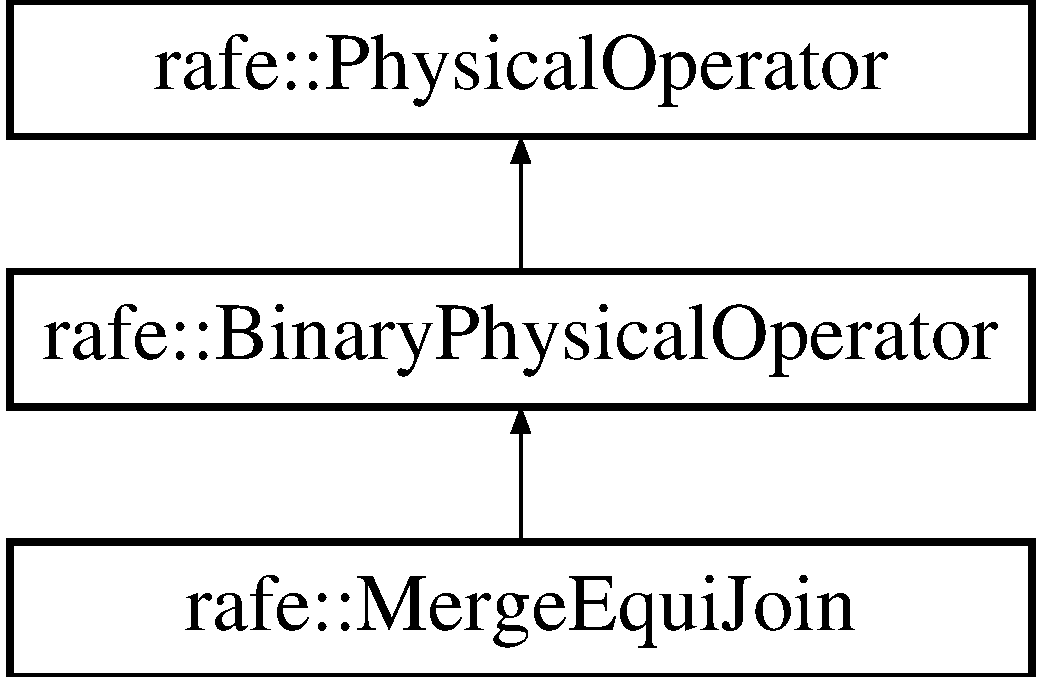
\includegraphics[height=3.000000cm]{classrafe_1_1_merge_equi_join}
\end{center}
\end{figure}
\subsection*{Public Member Functions}
\begin{DoxyCompactItemize}
\item 
\hyperlink{classrafe_1_1_merge_equi_join_ab51232a08c11f2f8402fffeafa7b4ea5}{Merge\+Equi\+Join} (const std\+::shared\+\_\+ptr$<$ \hyperlink{classrafe_1_1_expression}{Expression} $>$ \&\hyperlink{classrafe_1_1_merge_equi_join_a7b3cbe4e5b568582281f89de0eee0460}{condition})
\item 
void \hyperlink{classrafe_1_1_merge_equi_join_a612f15e10eb741126e282b605fef0921}{accept} (\hyperlink{classrafe_1_1_physical_operator_visitor}{Physical\+Operator\+Visitor} \&v)
\end{DoxyCompactItemize}
\subsection*{Public Attributes}
\begin{DoxyCompactItemize}
\item 
std\+::shared\+\_\+ptr$<$ \hyperlink{classrafe_1_1_expression}{Expression} $>$ \hyperlink{classrafe_1_1_merge_equi_join_a7b3cbe4e5b568582281f89de0eee0460}{condition}
\item 
std\+::vector$<$ \hyperlink{classrafe_1_1_sort_parameter}{Sort\+Parameter} $>$ \hyperlink{classrafe_1_1_merge_equi_join_adff0e135df404e746d1ddfac4ac25a8d}{left}
\item 
std\+::vector$<$ \hyperlink{classrafe_1_1_sort_parameter}{Sort\+Parameter} $>$ \hyperlink{classrafe_1_1_merge_equi_join_a3d77a9923ebd3aafe2aaf87fdf81bf6e}{right}
\end{DoxyCompactItemize}


\subsection{Detailed Description}
Represents merge equi join. Operator computes equijoin from given sorted inputs. 

\subsection{Constructor \& Destructor Documentation}
\hypertarget{classrafe_1_1_merge_equi_join_ab51232a08c11f2f8402fffeafa7b4ea5}{\index{rafe\+::\+Merge\+Equi\+Join@{rafe\+::\+Merge\+Equi\+Join}!Merge\+Equi\+Join@{Merge\+Equi\+Join}}
\index{Merge\+Equi\+Join@{Merge\+Equi\+Join}!rafe\+::\+Merge\+Equi\+Join@{rafe\+::\+Merge\+Equi\+Join}}
\subsubsection[{Merge\+Equi\+Join}]{\setlength{\rightskip}{0pt plus 5cm}rafe\+::\+Merge\+Equi\+Join\+::\+Merge\+Equi\+Join (
\begin{DoxyParamCaption}
\item[{const std\+::shared\+\_\+ptr$<$ {\bf Expression} $>$ \&}]{condition}
\end{DoxyParamCaption}
)}}\label{classrafe_1_1_merge_equi_join_ab51232a08c11f2f8402fffeafa7b4ea5}
Creates new instance of \hyperlink{classrafe_1_1_merge_equi_join}{Merge\+Equi\+Join}. 
\begin{DoxyParams}{Parameters}
{\em condition} & -\/ join condition. \\
\hline
\end{DoxyParams}


\subsection{Member Function Documentation}
\hypertarget{classrafe_1_1_merge_equi_join_a612f15e10eb741126e282b605fef0921}{\index{rafe\+::\+Merge\+Equi\+Join@{rafe\+::\+Merge\+Equi\+Join}!accept@{accept}}
\index{accept@{accept}!rafe\+::\+Merge\+Equi\+Join@{rafe\+::\+Merge\+Equi\+Join}}
\subsubsection[{accept}]{\setlength{\rightskip}{0pt plus 5cm}void rafe\+::\+Merge\+Equi\+Join\+::accept (
\begin{DoxyParamCaption}
\item[{{\bf Physical\+Operator\+Visitor} \&}]{v}
\end{DoxyParamCaption}
)\hspace{0.3cm}{\ttfamily [virtual]}}}\label{classrafe_1_1_merge_equi_join_a612f15e10eb741126e282b605fef0921}
Method for calling visit\mbox{[}node\mbox{]} on given \hyperlink{classrafe_1_1_physical_operator_visitor}{Physical\+Operator\+Visitor}. 
\begin{DoxyParams}{Parameters}
{\em v} & \hyperlink{classrafe_1_1_physical_operator_visitor}{Physical\+Operator\+Visitor}, on which to call function. \\
\hline
\end{DoxyParams}


Implements \hyperlink{classrafe_1_1_binary_physical_operator_a58ce0a14b970b2c932254419877a2e0e}{rafe\+::\+Binary\+Physical\+Operator}.



\subsection{Member Data Documentation}
\hypertarget{classrafe_1_1_merge_equi_join_a7b3cbe4e5b568582281f89de0eee0460}{\index{rafe\+::\+Merge\+Equi\+Join@{rafe\+::\+Merge\+Equi\+Join}!condition@{condition}}
\index{condition@{condition}!rafe\+::\+Merge\+Equi\+Join@{rafe\+::\+Merge\+Equi\+Join}}
\subsubsection[{condition}]{\setlength{\rightskip}{0pt plus 5cm}std\+::shared\+\_\+ptr$<${\bf Expression}$>$ rafe\+::\+Merge\+Equi\+Join\+::condition}}\label{classrafe_1_1_merge_equi_join_a7b3cbe4e5b568582281f89de0eee0460}
\hyperlink{classrafe_1_1_join}{Join} condition. \hypertarget{classrafe_1_1_merge_equi_join_adff0e135df404e746d1ddfac4ac25a8d}{\index{rafe\+::\+Merge\+Equi\+Join@{rafe\+::\+Merge\+Equi\+Join}!left@{left}}
\index{left@{left}!rafe\+::\+Merge\+Equi\+Join@{rafe\+::\+Merge\+Equi\+Join}}
\subsubsection[{left}]{\setlength{\rightskip}{0pt plus 5cm}std\+::vector$<${\bf Sort\+Parameter}$>$ rafe\+::\+Merge\+Equi\+Join\+::left}}\label{classrafe_1_1_merge_equi_join_adff0e135df404e746d1ddfac4ac25a8d}
Stored information how first input is sorted. \hypertarget{classrafe_1_1_merge_equi_join_a3d77a9923ebd3aafe2aaf87fdf81bf6e}{\index{rafe\+::\+Merge\+Equi\+Join@{rafe\+::\+Merge\+Equi\+Join}!right@{right}}
\index{right@{right}!rafe\+::\+Merge\+Equi\+Join@{rafe\+::\+Merge\+Equi\+Join}}
\subsubsection[{right}]{\setlength{\rightskip}{0pt plus 5cm}std\+::vector$<${\bf Sort\+Parameter}$>$ rafe\+::\+Merge\+Equi\+Join\+::right}}\label{classrafe_1_1_merge_equi_join_a3d77a9923ebd3aafe2aaf87fdf81bf6e}
Stored information how second input is sorted. 

The documentation for this class was generated from the following files\+:\begin{DoxyCompactItemize}
\item 
C\+:/\+Users/\+Marcel/\+Documents/\+Visual Studio 2012/\+Projects/\+Relational\+Query\+Evaluator/\+Relational\+Query\+Evaluator/Physical\+Operator.\+h\item 
C\+:/\+Users/\+Marcel/\+Documents/\+Visual Studio 2012/\+Projects/\+Relational\+Query\+Evaluator/\+Relational\+Query\+Evaluator/Physical\+Operator.\+cpp\end{DoxyCompactItemize}

\hypertarget{classrafe_1_1_merge_non_equi_join}{\section{rafe\+:\+:Merge\+Non\+Equi\+Join Class Reference}
\label{classrafe_1_1_merge_non_equi_join}\index{rafe\+::\+Merge\+Non\+Equi\+Join@{rafe\+::\+Merge\+Non\+Equi\+Join}}
}


{\ttfamily \#include $<$Physical\+Operator.\+h$>$}

Inheritance diagram for rafe\+:\+:Merge\+Non\+Equi\+Join\+:\begin{figure}[H]
\begin{center}
\leavevmode
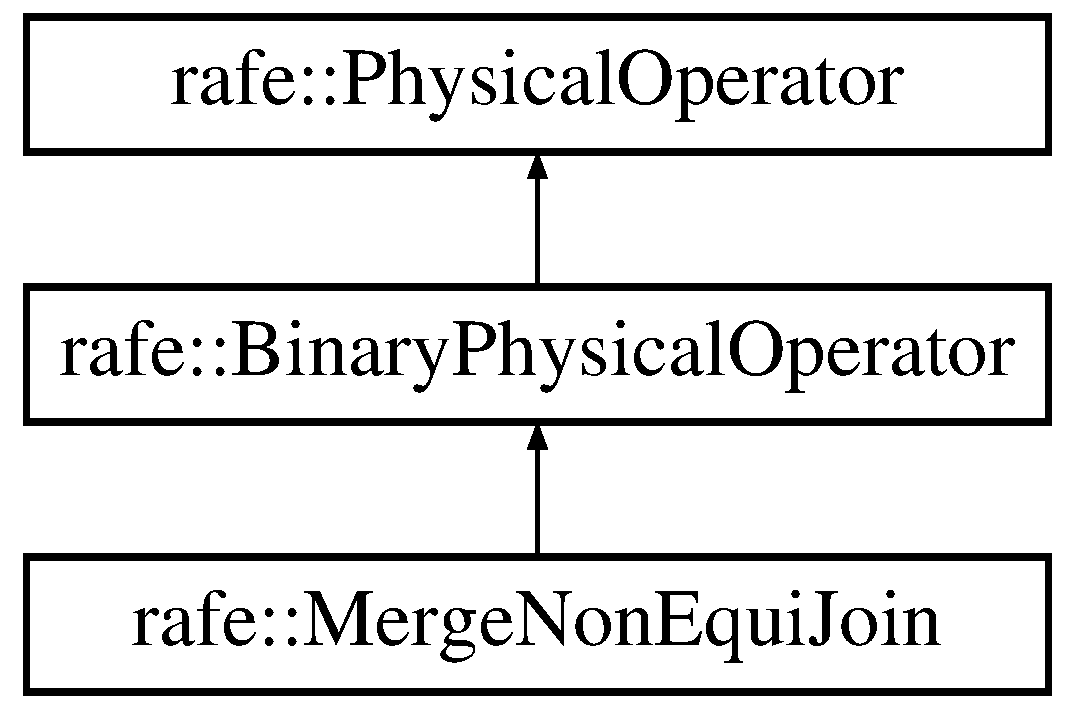
\includegraphics[height=3.000000cm]{classrafe_1_1_merge_non_equi_join}
\end{center}
\end{figure}
\subsection*{Public Member Functions}
\begin{DoxyCompactItemize}
\item 
\hyperlink{classrafe_1_1_merge_non_equi_join_addb7efb09c776ceb11250748001041ca}{Merge\+Non\+Equi\+Join} (const std\+::shared\+\_\+ptr$<$ \hyperlink{classrafe_1_1_expression}{Expression} $>$ \&\hyperlink{classrafe_1_1_merge_non_equi_join_a9082928b98835f698363bba69a77ffbe}{condition})
\item 
void \hyperlink{classrafe_1_1_merge_non_equi_join_a3accb9ad7ae5851370152885c23c6048}{accept} (\hyperlink{classrafe_1_1_physical_operator_visitor}{Physical\+Operator\+Visitor} \&v)
\end{DoxyCompactItemize}
\subsection*{Public Attributes}
\begin{DoxyCompactItemize}
\item 
std\+::shared\+\_\+ptr$<$ \hyperlink{classrafe_1_1_expression}{Expression} $>$ \hyperlink{classrafe_1_1_merge_non_equi_join_a9082928b98835f698363bba69a77ffbe}{condition}
\item 
std\+::vector$<$ \hyperlink{classrafe_1_1_sort_parameter}{Sort\+Parameter} $>$ \hyperlink{classrafe_1_1_merge_non_equi_join_af33e57260541cc8d7bda1905e2145983}{sort\+Parameters}
\item 
std\+::vector$<$ \hyperlink{classrafe_1_1_sort_parameter}{Sort\+Parameter} $>$ \hyperlink{classrafe_1_1_merge_non_equi_join_acbef8c68400bc4f58acdad98e3457545}{left}
\item 
std\+::vector$<$ \hyperlink{classrafe_1_1_sort_parameter}{Sort\+Parameter} $>$ \hyperlink{classrafe_1_1_merge_non_equi_join_a7083c038cc58409fc535d46f82633d6a}{right}
\end{DoxyCompactItemize}


\subsection{Detailed Description}
Represents merge join joining by condition a1 $<$ b $<$ a2, where a1 and a2 are columns from 1st input, b is from 2nd input. 

\subsection{Constructor \& Destructor Documentation}
\hypertarget{classrafe_1_1_merge_non_equi_join_addb7efb09c776ceb11250748001041ca}{\index{rafe\+::\+Merge\+Non\+Equi\+Join@{rafe\+::\+Merge\+Non\+Equi\+Join}!Merge\+Non\+Equi\+Join@{Merge\+Non\+Equi\+Join}}
\index{Merge\+Non\+Equi\+Join@{Merge\+Non\+Equi\+Join}!rafe\+::\+Merge\+Non\+Equi\+Join@{rafe\+::\+Merge\+Non\+Equi\+Join}}
\subsubsection[{Merge\+Non\+Equi\+Join}]{\setlength{\rightskip}{0pt plus 5cm}rafe\+::\+Merge\+Non\+Equi\+Join\+::\+Merge\+Non\+Equi\+Join (
\begin{DoxyParamCaption}
\item[{const std\+::shared\+\_\+ptr$<$ {\bf Expression} $>$ \&}]{condition}
\end{DoxyParamCaption}
)}}\label{classrafe_1_1_merge_non_equi_join_addb7efb09c776ceb11250748001041ca}
Creates new instance of \hyperlink{classrafe_1_1_merge_non_equi_join}{Merge\+Non\+Equi\+Join}. 
\begin{DoxyParams}{Parameters}
{\em condition} & -\/ join condition. \\
\hline
\end{DoxyParams}


\subsection{Member Function Documentation}
\hypertarget{classrafe_1_1_merge_non_equi_join_a3accb9ad7ae5851370152885c23c6048}{\index{rafe\+::\+Merge\+Non\+Equi\+Join@{rafe\+::\+Merge\+Non\+Equi\+Join}!accept@{accept}}
\index{accept@{accept}!rafe\+::\+Merge\+Non\+Equi\+Join@{rafe\+::\+Merge\+Non\+Equi\+Join}}
\subsubsection[{accept}]{\setlength{\rightskip}{0pt plus 5cm}void rafe\+::\+Merge\+Non\+Equi\+Join\+::accept (
\begin{DoxyParamCaption}
\item[{{\bf Physical\+Operator\+Visitor} \&}]{v}
\end{DoxyParamCaption}
)\hspace{0.3cm}{\ttfamily [virtual]}}}\label{classrafe_1_1_merge_non_equi_join_a3accb9ad7ae5851370152885c23c6048}
Method for calling visit\mbox{[}node\mbox{]} on given \hyperlink{classrafe_1_1_physical_operator_visitor}{Physical\+Operator\+Visitor}. 
\begin{DoxyParams}{Parameters}
{\em v} & \hyperlink{classrafe_1_1_physical_operator_visitor}{Physical\+Operator\+Visitor}, on which to call function. \\
\hline
\end{DoxyParams}


Implements \hyperlink{classrafe_1_1_binary_physical_operator_a58ce0a14b970b2c932254419877a2e0e}{rafe\+::\+Binary\+Physical\+Operator}.



\subsection{Member Data Documentation}
\hypertarget{classrafe_1_1_merge_non_equi_join_a9082928b98835f698363bba69a77ffbe}{\index{rafe\+::\+Merge\+Non\+Equi\+Join@{rafe\+::\+Merge\+Non\+Equi\+Join}!condition@{condition}}
\index{condition@{condition}!rafe\+::\+Merge\+Non\+Equi\+Join@{rafe\+::\+Merge\+Non\+Equi\+Join}}
\subsubsection[{condition}]{\setlength{\rightskip}{0pt plus 5cm}std\+::shared\+\_\+ptr$<${\bf Expression}$>$ rafe\+::\+Merge\+Non\+Equi\+Join\+::condition}}\label{classrafe_1_1_merge_non_equi_join_a9082928b98835f698363bba69a77ffbe}
\hyperlink{classrafe_1_1_join}{Join} condition. \hypertarget{classrafe_1_1_merge_non_equi_join_acbef8c68400bc4f58acdad98e3457545}{\index{rafe\+::\+Merge\+Non\+Equi\+Join@{rafe\+::\+Merge\+Non\+Equi\+Join}!left@{left}}
\index{left@{left}!rafe\+::\+Merge\+Non\+Equi\+Join@{rafe\+::\+Merge\+Non\+Equi\+Join}}
\subsubsection[{left}]{\setlength{\rightskip}{0pt plus 5cm}std\+::vector$<${\bf Sort\+Parameter}$>$ rafe\+::\+Merge\+Non\+Equi\+Join\+::left}}\label{classrafe_1_1_merge_non_equi_join_acbef8c68400bc4f58acdad98e3457545}
Stored information how first input is sorted. \hypertarget{classrafe_1_1_merge_non_equi_join_a7083c038cc58409fc535d46f82633d6a}{\index{rafe\+::\+Merge\+Non\+Equi\+Join@{rafe\+::\+Merge\+Non\+Equi\+Join}!right@{right}}
\index{right@{right}!rafe\+::\+Merge\+Non\+Equi\+Join@{rafe\+::\+Merge\+Non\+Equi\+Join}}
\subsubsection[{right}]{\setlength{\rightskip}{0pt plus 5cm}std\+::vector$<${\bf Sort\+Parameter}$>$ rafe\+::\+Merge\+Non\+Equi\+Join\+::right}}\label{classrafe_1_1_merge_non_equi_join_a7083c038cc58409fc535d46f82633d6a}
Stored information how second input is sorted. \hypertarget{classrafe_1_1_merge_non_equi_join_af33e57260541cc8d7bda1905e2145983}{\index{rafe\+::\+Merge\+Non\+Equi\+Join@{rafe\+::\+Merge\+Non\+Equi\+Join}!sort\+Parameters@{sort\+Parameters}}
\index{sort\+Parameters@{sort\+Parameters}!rafe\+::\+Merge\+Non\+Equi\+Join@{rafe\+::\+Merge\+Non\+Equi\+Join}}
\subsubsection[{sort\+Parameters}]{\setlength{\rightskip}{0pt plus 5cm}std\+::vector$<${\bf Sort\+Parameter}$>$ rafe\+::\+Merge\+Non\+Equi\+Join\+::sort\+Parameters}}\label{classrafe_1_1_merge_non_equi_join_af33e57260541cc8d7bda1905e2145983}
Stored information how output is sorted. 

The documentation for this class was generated from the following files\+:\begin{DoxyCompactItemize}
\item 
C\+:/\+Users/\+Marcel/\+Documents/\+Visual Studio 2012/\+Projects/\+Relational\+Query\+Evaluator/\+Relational\+Query\+Evaluator/Physical\+Operator.\+h\item 
C\+:/\+Users/\+Marcel/\+Documents/\+Visual Studio 2012/\+Projects/\+Relational\+Query\+Evaluator/\+Relational\+Query\+Evaluator/Physical\+Operator.\+cpp\end{DoxyCompactItemize}

\hypertarget{classrafe_1_1_nnary_expression}{\section{rafe\+:\+:Nnary\+Expression Class Reference}
\label{classrafe_1_1_nnary_expression}\index{rafe\+::\+Nnary\+Expression@{rafe\+::\+Nnary\+Expression}}
}


{\ttfamily \#include $<$Expressions.\+h$>$}

Inheritance diagram for rafe\+:\+:Nnary\+Expression\+:\begin{figure}[H]
\begin{center}
\leavevmode
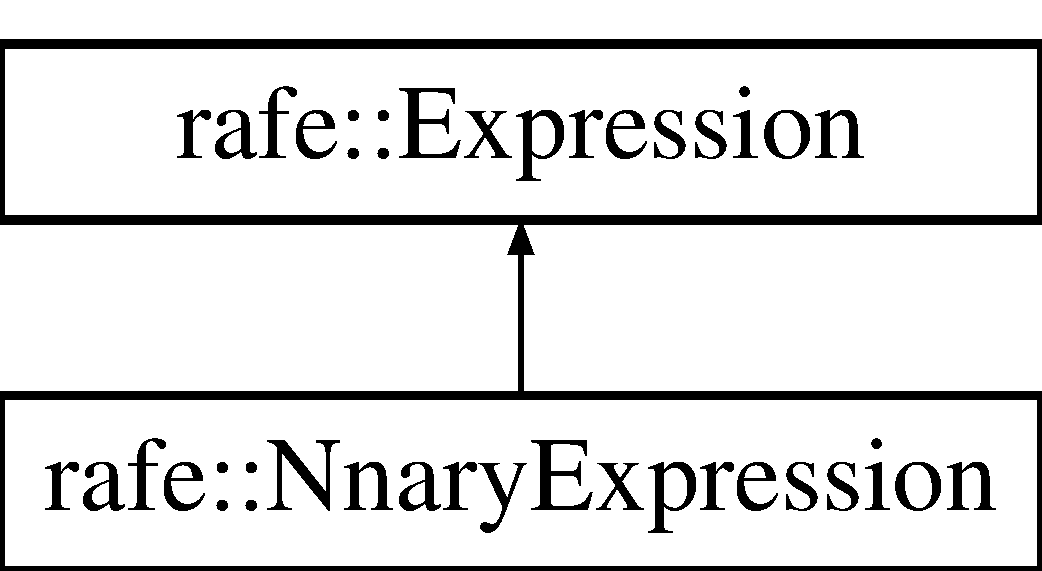
\includegraphics[height=2.000000cm]{classrafe_1_1_nnary_expression}
\end{center}
\end{figure}
\subsection*{Public Member Functions}
\begin{DoxyCompactItemize}
\item 
\hyperlink{classrafe_1_1_nnary_expression_ab136f6b504e0c3523bd2e6a929022d58}{Nnary\+Expression} (D\+O\+M\+Element $\ast$node, const std\+::string \&\hyperlink{classrafe_1_1_nnary_expression_a14fbf6f0dd20a40e6ea647a1223e5362}{name}, const std\+::string \&\hyperlink{classrafe_1_1_nnary_expression_a220fa9d75003ecbadc3c3b365e5c8603}{return\+Type})
\item 
void \hyperlink{classrafe_1_1_nnary_expression_a69364332f3ee37e38901cdef923c6eeb}{accept} (\hyperlink{classrafe_1_1_expression_visitor_base}{Expression\+Visitor\+Base} \&v)
\item 
void \hyperlink{classrafe_1_1_nnary_expression_a3e7adc7e9dc45caa0a6ac3919564a921}{replace\+Child} (\hyperlink{classrafe_1_1_expression}{Expression} $\ast$old\+Child, std\+::shared\+\_\+ptr$<$ \hyperlink{classrafe_1_1_expression}{Expression} $>$ new\+Child)
\end{DoxyCompactItemize}
\subsection*{Public Attributes}
\begin{DoxyCompactItemize}
\item 
std\+::string \hyperlink{classrafe_1_1_nnary_expression_a14fbf6f0dd20a40e6ea647a1223e5362}{name}
\item 
std\+::string \hyperlink{classrafe_1_1_nnary_expression_a220fa9d75003ecbadc3c3b365e5c8603}{return\+Type}
\item 
std\+::vector$<$ std\+::shared\+\_\+ptr\\*
$<$ \hyperlink{classrafe_1_1_expression}{Expression} $>$ $>$ \hyperlink{classrafe_1_1_nnary_expression_af78598eb1a4c75a90204a85aa2292313}{arguments}
\end{DoxyCompactItemize}
\subsection*{Additional Inherited Members}


\subsection{Detailed Description}
Represents co called n-\/nary expresion, it is a function call with variable argument number. N-\/nary expression can be for expample sql function like or date or arithmetic function sqrt 

\subsection{Constructor \& Destructor Documentation}
\hypertarget{classrafe_1_1_nnary_expression_ab136f6b504e0c3523bd2e6a929022d58}{\index{rafe\+::\+Nnary\+Expression@{rafe\+::\+Nnary\+Expression}!Nnary\+Expression@{Nnary\+Expression}}
\index{Nnary\+Expression@{Nnary\+Expression}!rafe\+::\+Nnary\+Expression@{rafe\+::\+Nnary\+Expression}}
\subsubsection[{Nnary\+Expression}]{\setlength{\rightskip}{0pt plus 5cm}rafe\+::\+Nnary\+Expression\+::\+Nnary\+Expression (
\begin{DoxyParamCaption}
\item[{D\+O\+M\+Element $\ast$}]{node, }
\item[{const std\+::string \&}]{name, }
\item[{const std\+::string \&}]{return\+Type}
\end{DoxyParamCaption}
)}}\label{classrafe_1_1_nnary_expression_ab136f6b504e0c3523bd2e6a929022d58}
Creates new instace of \hyperlink{classrafe_1_1_nnary_expression}{Nnary\+Expression}. 
\begin{DoxyParams}{Parameters}
{\em node} & -\/ element containing infromation about node and it's children \\
\hline
{\em name} & -\/ function name \\
\hline
{\em return\+Type} & -\/ return type of function \\
\hline
\end{DoxyParams}


\subsection{Member Function Documentation}
\hypertarget{classrafe_1_1_nnary_expression_a69364332f3ee37e38901cdef923c6eeb}{\index{rafe\+::\+Nnary\+Expression@{rafe\+::\+Nnary\+Expression}!accept@{accept}}
\index{accept@{accept}!rafe\+::\+Nnary\+Expression@{rafe\+::\+Nnary\+Expression}}
\subsubsection[{accept}]{\setlength{\rightskip}{0pt plus 5cm}void rafe\+::\+Nnary\+Expression\+::accept (
\begin{DoxyParamCaption}
\item[{{\bf Expression\+Visitor\+Base} \&}]{v}
\end{DoxyParamCaption}
)\hspace{0.3cm}{\ttfamily [virtual]}}}\label{classrafe_1_1_nnary_expression_a69364332f3ee37e38901cdef923c6eeb}
Method for calling visit\mbox{[}node\mbox{]} on given Expression\+Visitor. 
\begin{DoxyParams}{Parameters}
{\em v} & Expression\+Visitor, on which to call visit function. \\
\hline
\end{DoxyParams}


Implements \hyperlink{classrafe_1_1_expression_a3b2e5bae8b99ea6c9a3c92a9b949b3cd}{rafe\+::\+Expression}.

\hypertarget{classrafe_1_1_nnary_expression_a3e7adc7e9dc45caa0a6ac3919564a921}{\index{rafe\+::\+Nnary\+Expression@{rafe\+::\+Nnary\+Expression}!replace\+Child@{replace\+Child}}
\index{replace\+Child@{replace\+Child}!rafe\+::\+Nnary\+Expression@{rafe\+::\+Nnary\+Expression}}
\subsubsection[{replace\+Child}]{\setlength{\rightskip}{0pt plus 5cm}void rafe\+::\+Nnary\+Expression\+::replace\+Child (
\begin{DoxyParamCaption}
\item[{{\bf Expression} $\ast$}]{old\+Child, }
\item[{std\+::shared\+\_\+ptr$<$ {\bf Expression} $>$}]{new\+Child}
\end{DoxyParamCaption}
)\hspace{0.3cm}{\ttfamily [virtual]}}}\label{classrafe_1_1_nnary_expression_a3e7adc7e9dc45caa0a6ac3919564a921}
Replaces child from this class with new expression tree. 
\begin{DoxyParams}{Parameters}
{\em old\+Child} & -\/ child to replace. \\
\hline
{\em new\+Child} & -\/ child to be replaced. \\
\hline
\end{DoxyParams}


Implements \hyperlink{classrafe_1_1_expression_a841879e8eb85f4bb68cfeec24231a701}{rafe\+::\+Expression}.



\subsection{Member Data Documentation}
\hypertarget{classrafe_1_1_nnary_expression_af78598eb1a4c75a90204a85aa2292313}{\index{rafe\+::\+Nnary\+Expression@{rafe\+::\+Nnary\+Expression}!arguments@{arguments}}
\index{arguments@{arguments}!rafe\+::\+Nnary\+Expression@{rafe\+::\+Nnary\+Expression}}
\subsubsection[{arguments}]{\setlength{\rightskip}{0pt plus 5cm}std\+::vector$<$std\+::shared\+\_\+ptr$<${\bf Expression}$>$ $>$ rafe\+::\+Nnary\+Expression\+::arguments}}\label{classrafe_1_1_nnary_expression_af78598eb1a4c75a90204a85aa2292313}
Stores call arguments. Arguments are also expression trees. \hypertarget{classrafe_1_1_nnary_expression_a14fbf6f0dd20a40e6ea647a1223e5362}{\index{rafe\+::\+Nnary\+Expression@{rafe\+::\+Nnary\+Expression}!name@{name}}
\index{name@{name}!rafe\+::\+Nnary\+Expression@{rafe\+::\+Nnary\+Expression}}
\subsubsection[{name}]{\setlength{\rightskip}{0pt plus 5cm}std\+::string rafe\+::\+Nnary\+Expression\+::name}}\label{classrafe_1_1_nnary_expression_a14fbf6f0dd20a40e6ea647a1223e5362}
Stores function name. \hypertarget{classrafe_1_1_nnary_expression_a220fa9d75003ecbadc3c3b365e5c8603}{\index{rafe\+::\+Nnary\+Expression@{rafe\+::\+Nnary\+Expression}!return\+Type@{return\+Type}}
\index{return\+Type@{return\+Type}!rafe\+::\+Nnary\+Expression@{rafe\+::\+Nnary\+Expression}}
\subsubsection[{return\+Type}]{\setlength{\rightskip}{0pt plus 5cm}std\+::string rafe\+::\+Nnary\+Expression\+::return\+Type}}\label{classrafe_1_1_nnary_expression_a220fa9d75003ecbadc3c3b365e5c8603}
Stores function return type. 

The documentation for this class was generated from the following files\+:\begin{DoxyCompactItemize}
\item 
C\+:/\+Users/\+Marcel/\+Documents/\+Visual Studio 2012/\+Projects/\+Relational\+Query\+Evaluator/\+Relational\+Query\+Evaluator/Expressions.\+h\item 
C\+:/\+Users/\+Marcel/\+Documents/\+Visual Studio 2012/\+Projects/\+Relational\+Query\+Evaluator/\+Relational\+Query\+Evaluator/Expressions.\+cpp\end{DoxyCompactItemize}

\hypertarget{classrafe_1_1_nullary_algebra_node_base}{\section{rafe\+:\+:Nullary\+Algebra\+Node\+Base Class Reference}
\label{classrafe_1_1_nullary_algebra_node_base}\index{rafe\+::\+Nullary\+Algebra\+Node\+Base@{rafe\+::\+Nullary\+Algebra\+Node\+Base}}
}


{\ttfamily \#include $<$Algebra.\+h$>$}

Inheritance diagram for rafe\+:\+:Nullary\+Algebra\+Node\+Base\+:\begin{figure}[H]
\begin{center}
\leavevmode
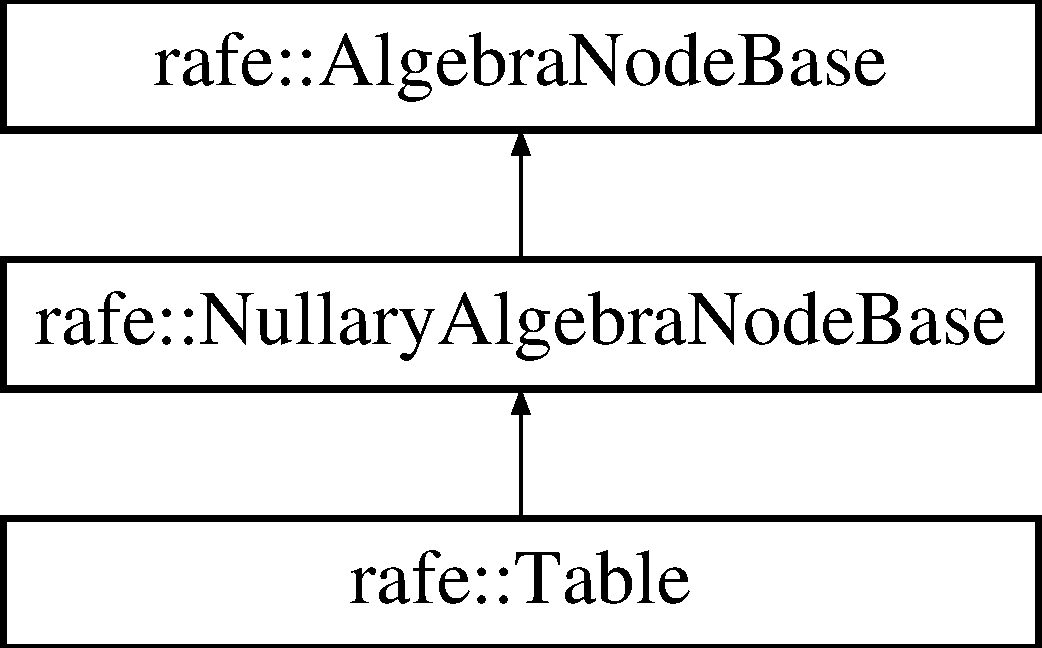
\includegraphics[height=3.000000cm]{classrafe_1_1_nullary_algebra_node_base}
\end{center}
\end{figure}
\subsection*{Public Member Functions}
\begin{DoxyCompactItemize}
\item 
\hyperlink{classrafe_1_1_nullary_algebra_node_base_ad27b12a11492ddc6d3d07f1781e0dfcf}{Nullary\+Algebra\+Node\+Base} (D\+O\+M\+Element $\ast$element)
\item 
virtual void \hyperlink{classrafe_1_1_nullary_algebra_node_base_a4e1bc16e76d9e41a8fb575008d8f15e5}{accept} (\hyperlink{classrafe_1_1_algebra_visitor}{Algebra\+Visitor} \&v)=0
\item 
std\+::shared\+\_\+ptr$<$ \hyperlink{classrafe_1_1_algebra_node_base}{Algebra\+Node\+Base} $>$ \hyperlink{classrafe_1_1_nullary_algebra_node_base_aa600eac4377bac4699834b0fbf1a4051}{replace\+Child} (\hyperlink{classrafe_1_1_algebra_node_base}{Algebra\+Node\+Base} $\ast$old\+Child, std\+::shared\+\_\+ptr$<$ \hyperlink{classrafe_1_1_algebra_node_base}{Algebra\+Node\+Base} $>$ \&new\+Child)
\end{DoxyCompactItemize}
\subsection*{Additional Inherited Members}


\subsection{Detailed Description}
Abstract class for nullary algebraic operation. 

\subsection{Constructor \& Destructor Documentation}
\hypertarget{classrafe_1_1_nullary_algebra_node_base_ad27b12a11492ddc6d3d07f1781e0dfcf}{\index{rafe\+::\+Nullary\+Algebra\+Node\+Base@{rafe\+::\+Nullary\+Algebra\+Node\+Base}!Nullary\+Algebra\+Node\+Base@{Nullary\+Algebra\+Node\+Base}}
\index{Nullary\+Algebra\+Node\+Base@{Nullary\+Algebra\+Node\+Base}!rafe\+::\+Nullary\+Algebra\+Node\+Base@{rafe\+::\+Nullary\+Algebra\+Node\+Base}}
\subsubsection[{Nullary\+Algebra\+Node\+Base}]{\setlength{\rightskip}{0pt plus 5cm}rafe\+::\+Nullary\+Algebra\+Node\+Base\+::\+Nullary\+Algebra\+Node\+Base (
\begin{DoxyParamCaption}
\item[{D\+O\+M\+Element $\ast$}]{element}
\end{DoxyParamCaption}
)}}\label{classrafe_1_1_nullary_algebra_node_base_ad27b12a11492ddc6d3d07f1781e0dfcf}
Creates the instance of \hyperlink{classrafe_1_1_nullary_algebra_node_base}{Nullary\+Algebra\+Node\+Base}. 
\begin{DoxyParams}{Parameters}
{\em element} & representing input node. \\
\hline
\end{DoxyParams}


\subsection{Member Function Documentation}
\hypertarget{classrafe_1_1_nullary_algebra_node_base_a4e1bc16e76d9e41a8fb575008d8f15e5}{\index{rafe\+::\+Nullary\+Algebra\+Node\+Base@{rafe\+::\+Nullary\+Algebra\+Node\+Base}!accept@{accept}}
\index{accept@{accept}!rafe\+::\+Nullary\+Algebra\+Node\+Base@{rafe\+::\+Nullary\+Algebra\+Node\+Base}}
\subsubsection[{accept}]{\setlength{\rightskip}{0pt plus 5cm}virtual void rafe\+::\+Nullary\+Algebra\+Node\+Base\+::accept (
\begin{DoxyParamCaption}
\item[{{\bf Algebra\+Visitor} \&}]{v}
\end{DoxyParamCaption}
)\hspace{0.3cm}{\ttfamily [pure virtual]}}}\label{classrafe_1_1_nullary_algebra_node_base_a4e1bc16e76d9e41a8fb575008d8f15e5}
Method for calling visit\mbox{[}node\mbox{]} on given \hyperlink{classrafe_1_1_algebra_visitor}{Algebra\+Visitor}. 
\begin{DoxyParams}{Parameters}
{\em v} & \hyperlink{classrafe_1_1_algebra_visitor}{Algebra\+Visitor} on which to call function. \\
\hline
\end{DoxyParams}


Implements \hyperlink{classrafe_1_1_algebra_node_base_a48e59b55cdb1c3d108343eb18920c1d1}{rafe\+::\+Algebra\+Node\+Base}.



Implemented in \hyperlink{classrafe_1_1_table_a2a807fb6c8921673ba7adb62dd0a9f7c}{rafe\+::\+Table}.

\hypertarget{classrafe_1_1_nullary_algebra_node_base_aa600eac4377bac4699834b0fbf1a4051}{\index{rafe\+::\+Nullary\+Algebra\+Node\+Base@{rafe\+::\+Nullary\+Algebra\+Node\+Base}!replace\+Child@{replace\+Child}}
\index{replace\+Child@{replace\+Child}!rafe\+::\+Nullary\+Algebra\+Node\+Base@{rafe\+::\+Nullary\+Algebra\+Node\+Base}}
\subsubsection[{replace\+Child}]{\setlength{\rightskip}{0pt plus 5cm}shared\+\_\+ptr$<$ {\bf Algebra\+Node\+Base} $>$ rafe\+::\+Nullary\+Algebra\+Node\+Base\+::replace\+Child (
\begin{DoxyParamCaption}
\item[{{\bf Algebra\+Node\+Base} $\ast$}]{old\+Child, }
\item[{std\+::shared\+\_\+ptr$<$ {\bf Algebra\+Node\+Base} $>$ \&}]{new\+Child}
\end{DoxyParamCaption}
)\hspace{0.3cm}{\ttfamily [virtual]}}}\label{classrafe_1_1_nullary_algebra_node_base_aa600eac4377bac4699834b0fbf1a4051}
Replaces one child of this node with other one. 
\begin{DoxyParams}{Parameters}
{\em old\+Child} & node to be replaced. \\
\hline
{\em new\+Child} & new node to replace the old one. \\
\hline
\end{DoxyParams}
\begin{DoxyReturn}{Returns}
replaced child. 
\end{DoxyReturn}


Implements \hyperlink{classrafe_1_1_algebra_node_base_ac6d722e739dd39c223bb129dfbd0ab45}{rafe\+::\+Algebra\+Node\+Base}.



The documentation for this class was generated from the following files\+:\begin{DoxyCompactItemize}
\item 
C\+:/\+Users/\+Marcel/\+Documents/\+Visual Studio 2012/\+Projects/\+Relational\+Query\+Evaluator/\+Relational\+Query\+Evaluator/Algebra.\+h\item 
C\+:/\+Users/\+Marcel/\+Documents/\+Visual Studio 2012/\+Projects/\+Relational\+Query\+Evaluator/\+Relational\+Query\+Evaluator/Algebra.\+cpp\end{DoxyCompactItemize}

\hypertarget{classrafe_1_1_nullary_physical_operator}{\section{rafe\+:\+:Nullary\+Physical\+Operator Class Reference}
\label{classrafe_1_1_nullary_physical_operator}\index{rafe\+::\+Nullary\+Physical\+Operator@{rafe\+::\+Nullary\+Physical\+Operator}}
}


{\ttfamily \#include $<$Physical\+Operator.\+h$>$}

Inheritance diagram for rafe\+:\+:Nullary\+Physical\+Operator\+:\begin{figure}[H]
\begin{center}
\leavevmode
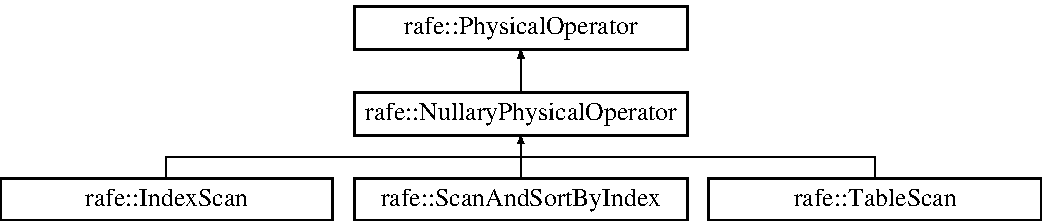
\includegraphics[height=2.962963cm]{classrafe_1_1_nullary_physical_operator}
\end{center}
\end{figure}
\subsection*{Public Member Functions}
\begin{DoxyCompactItemize}
\item 
virtual void \hyperlink{classrafe_1_1_nullary_physical_operator_a0810fc4b368521ebe847fa48fcdcf948}{accept} (\hyperlink{classrafe_1_1_physical_operator_visitor}{Physical\+Operator\+Visitor} \&v)=0
\end{DoxyCompactItemize}
\subsection*{Additional Inherited Members}


\subsection{Detailed Description}
Base class for operators with no input. It is used for leafs like read table, read table by index and index scan. 

\subsection{Member Function Documentation}
\hypertarget{classrafe_1_1_nullary_physical_operator_a0810fc4b368521ebe847fa48fcdcf948}{\index{rafe\+::\+Nullary\+Physical\+Operator@{rafe\+::\+Nullary\+Physical\+Operator}!accept@{accept}}
\index{accept@{accept}!rafe\+::\+Nullary\+Physical\+Operator@{rafe\+::\+Nullary\+Physical\+Operator}}
\subsubsection[{accept}]{\setlength{\rightskip}{0pt plus 5cm}virtual void rafe\+::\+Nullary\+Physical\+Operator\+::accept (
\begin{DoxyParamCaption}
\item[{{\bf Physical\+Operator\+Visitor} \&}]{v}
\end{DoxyParamCaption}
)\hspace{0.3cm}{\ttfamily [pure virtual]}}}\label{classrafe_1_1_nullary_physical_operator_a0810fc4b368521ebe847fa48fcdcf948}
Method for calling visit\mbox{[}node\mbox{]} on given \hyperlink{classrafe_1_1_physical_operator_visitor}{Physical\+Operator\+Visitor}. 
\begin{DoxyParams}{Parameters}
{\em v} & \hyperlink{classrafe_1_1_physical_operator_visitor}{Physical\+Operator\+Visitor}, on which to call function. \\
\hline
\end{DoxyParams}


Implements \hyperlink{classrafe_1_1_physical_operator_a263a89f54604263cea897c5adf8944a3}{rafe\+::\+Physical\+Operator}.



Implemented in \hyperlink{classrafe_1_1_index_scan_a5e4e26317258097176b3b3b241653302}{rafe\+::\+Index\+Scan}, \hyperlink{classrafe_1_1_table_scan_a87cd9f9b093f153bd95b39bc3ea18678}{rafe\+::\+Table\+Scan}, and \hyperlink{classrafe_1_1_scan_and_sort_by_index_aabb5d931b679a14bde40a1928ac10a52}{rafe\+::\+Scan\+And\+Sort\+By\+Index}.



The documentation for this class was generated from the following file\+:\begin{DoxyCompactItemize}
\item 
C\+:/\+Users/\+Marcel/\+Documents/\+Visual Studio 2012/\+Projects/\+Relational\+Query\+Evaluator/\+Relational\+Query\+Evaluator/Physical\+Operator.\+h\end{DoxyCompactItemize}

\hypertarget{classrafe_1_1_number_columns_in_join_visitor}{\section{rafe\+:\+:Number\+Columns\+In\+Join\+Visitor Class Reference}
\label{classrafe_1_1_number_columns_in_join_visitor}\index{rafe\+::\+Number\+Columns\+In\+Join\+Visitor@{rafe\+::\+Number\+Columns\+In\+Join\+Visitor}}
}


{\ttfamily \#include $<$Expression\+Visitors.\+h$>$}

Inheritance diagram for rafe\+:\+:Number\+Columns\+In\+Join\+Visitor\+:\begin{figure}[H]
\begin{center}
\leavevmode
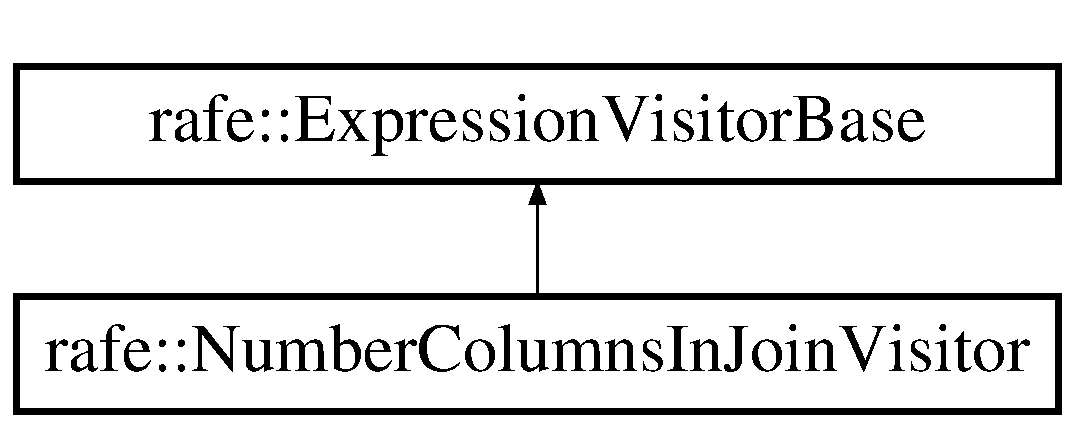
\includegraphics[height=2.000000cm]{classrafe_1_1_number_columns_in_join_visitor}
\end{center}
\end{figure}
\subsection*{Public Member Functions}
\begin{DoxyCompactItemize}
\item 
\hyperlink{classrafe_1_1_number_columns_in_join_visitor_a7139834faf5f6814ff8d48c05ec0f260}{Number\+Columns\+In\+Join\+Visitor} ()
\item 
void \hyperlink{classrafe_1_1_number_columns_in_join_visitor_a0a9ea8d0e184365f7f869452e13b8a63}{visit\+Column} (\hyperlink{classrafe_1_1_column}{Column} $\ast$expression)
\item 
void \hyperlink{classrafe_1_1_number_columns_in_join_visitor_a56c533c28f9948a6fcc0e8856a7b19e4}{visit\+Binary\+Expression} (\hyperlink{classrafe_1_1_binary_expression}{Binary\+Expression} $\ast$expression)
\end{DoxyCompactItemize}
\subsection*{Public Attributes}
\begin{DoxyCompactItemize}
\item 
int \hyperlink{classrafe_1_1_number_columns_in_join_visitor_a332114b3e616548b03a47c34e65f386a}{last\+Numbered\+Column}
\end{DoxyCompactItemize}


\subsection{Detailed Description}
Visitor which assign inout number to every column node. It is used in join and antijoin for identifying columns. 

\subsection{Constructor \& Destructor Documentation}
\hypertarget{classrafe_1_1_number_columns_in_join_visitor_a7139834faf5f6814ff8d48c05ec0f260}{\index{rafe\+::\+Number\+Columns\+In\+Join\+Visitor@{rafe\+::\+Number\+Columns\+In\+Join\+Visitor}!Number\+Columns\+In\+Join\+Visitor@{Number\+Columns\+In\+Join\+Visitor}}
\index{Number\+Columns\+In\+Join\+Visitor@{Number\+Columns\+In\+Join\+Visitor}!rafe\+::\+Number\+Columns\+In\+Join\+Visitor@{rafe\+::\+Number\+Columns\+In\+Join\+Visitor}}
\subsubsection[{Number\+Columns\+In\+Join\+Visitor}]{\setlength{\rightskip}{0pt plus 5cm}rafe\+::\+Number\+Columns\+In\+Join\+Visitor\+::\+Number\+Columns\+In\+Join\+Visitor (
\begin{DoxyParamCaption}
{}
\end{DoxyParamCaption}
)}}\label{classrafe_1_1_number_columns_in_join_visitor_a7139834faf5f6814ff8d48c05ec0f260}
Creates new instance of \hyperlink{classrafe_1_1_number_columns_in_join_visitor}{Number\+Columns\+In\+Join\+Visitor} 

\subsection{Member Function Documentation}
\hypertarget{classrafe_1_1_number_columns_in_join_visitor_a56c533c28f9948a6fcc0e8856a7b19e4}{\index{rafe\+::\+Number\+Columns\+In\+Join\+Visitor@{rafe\+::\+Number\+Columns\+In\+Join\+Visitor}!visit\+Binary\+Expression@{visit\+Binary\+Expression}}
\index{visit\+Binary\+Expression@{visit\+Binary\+Expression}!rafe\+::\+Number\+Columns\+In\+Join\+Visitor@{rafe\+::\+Number\+Columns\+In\+Join\+Visitor}}
\subsubsection[{visit\+Binary\+Expression}]{\setlength{\rightskip}{0pt plus 5cm}void rafe\+::\+Number\+Columns\+In\+Join\+Visitor\+::visit\+Binary\+Expression (
\begin{DoxyParamCaption}
\item[{{\bf Binary\+Expression} $\ast$}]{expression}
\end{DoxyParamCaption}
)\hspace{0.3cm}{\ttfamily [virtual]}}}\label{classrafe_1_1_number_columns_in_join_visitor_a56c533c28f9948a6fcc0e8856a7b19e4}
Visits \hyperlink{classrafe_1_1_binary_expression}{Binary\+Expression} element. 
\begin{DoxyParams}{Parameters}
{\em expression} & visited \hyperlink{classrafe_1_1_binary_expression}{Binary\+Expression}. \\
\hline
\end{DoxyParams}


Reimplemented from \hyperlink{classrafe_1_1_expression_visitor_base_a63e53276af3a22d3592f34d05ba97014}{rafe\+::\+Expression\+Visitor\+Base}.

\hypertarget{classrafe_1_1_number_columns_in_join_visitor_a0a9ea8d0e184365f7f869452e13b8a63}{\index{rafe\+::\+Number\+Columns\+In\+Join\+Visitor@{rafe\+::\+Number\+Columns\+In\+Join\+Visitor}!visit\+Column@{visit\+Column}}
\index{visit\+Column@{visit\+Column}!rafe\+::\+Number\+Columns\+In\+Join\+Visitor@{rafe\+::\+Number\+Columns\+In\+Join\+Visitor}}
\subsubsection[{visit\+Column}]{\setlength{\rightskip}{0pt plus 5cm}void rafe\+::\+Number\+Columns\+In\+Join\+Visitor\+::visit\+Column (
\begin{DoxyParamCaption}
\item[{{\bf Column} $\ast$}]{expression}
\end{DoxyParamCaption}
)\hspace{0.3cm}{\ttfamily [virtual]}}}\label{classrafe_1_1_number_columns_in_join_visitor_a0a9ea8d0e184365f7f869452e13b8a63}
Visits \hyperlink{classrafe_1_1_column}{Column} element. 
\begin{DoxyParams}{Parameters}
{\em expression} & visited \hyperlink{classrafe_1_1_column}{Column}. \\
\hline
\end{DoxyParams}


Reimplemented from \hyperlink{classrafe_1_1_expression_visitor_base_a4eaa77bf4105d1cbdde4feb047228255}{rafe\+::\+Expression\+Visitor\+Base}.



\subsection{Member Data Documentation}
\hypertarget{classrafe_1_1_number_columns_in_join_visitor_a332114b3e616548b03a47c34e65f386a}{\index{rafe\+::\+Number\+Columns\+In\+Join\+Visitor@{rafe\+::\+Number\+Columns\+In\+Join\+Visitor}!last\+Numbered\+Column@{last\+Numbered\+Column}}
\index{last\+Numbered\+Column@{last\+Numbered\+Column}!rafe\+::\+Number\+Columns\+In\+Join\+Visitor@{rafe\+::\+Number\+Columns\+In\+Join\+Visitor}}
\subsubsection[{last\+Numbered\+Column}]{\setlength{\rightskip}{0pt plus 5cm}int rafe\+::\+Number\+Columns\+In\+Join\+Visitor\+::last\+Numbered\+Column}}\label{classrafe_1_1_number_columns_in_join_visitor_a332114b3e616548b03a47c34e65f386a}
Contains only 0or 1. Columns from left join input are numbered 0, and from right join input are numbered 1. 

The documentation for this class was generated from the following files\+:\begin{DoxyCompactItemize}
\item 
C\+:/\+Users/\+Marcel/\+Documents/\+Visual Studio 2012/\+Projects/\+Relational\+Query\+Evaluator/\+Relational\+Query\+Evaluator/Expression\+Visitors.\+h\item 
C\+:/\+Users/\+Marcel/\+Documents/\+Visual Studio 2012/\+Projects/\+Relational\+Query\+Evaluator/\+Relational\+Query\+Evaluator/Expression\+Visitors.\+cpp\end{DoxyCompactItemize}

\hypertarget{classrafe_1_1_parser_error_handler}{\section{rafe\+:\+:Parser\+Error\+Handler Class Reference}
\label{classrafe_1_1_parser_error_handler}\index{rafe\+::\+Parser\+Error\+Handler@{rafe\+::\+Parser\+Error\+Handler}}
}


{\ttfamily \#include $<$Xml\+Handler.\+h$>$}

Inheritance diagram for rafe\+:\+:Parser\+Error\+Handler\+:\begin{figure}[H]
\begin{center}
\leavevmode
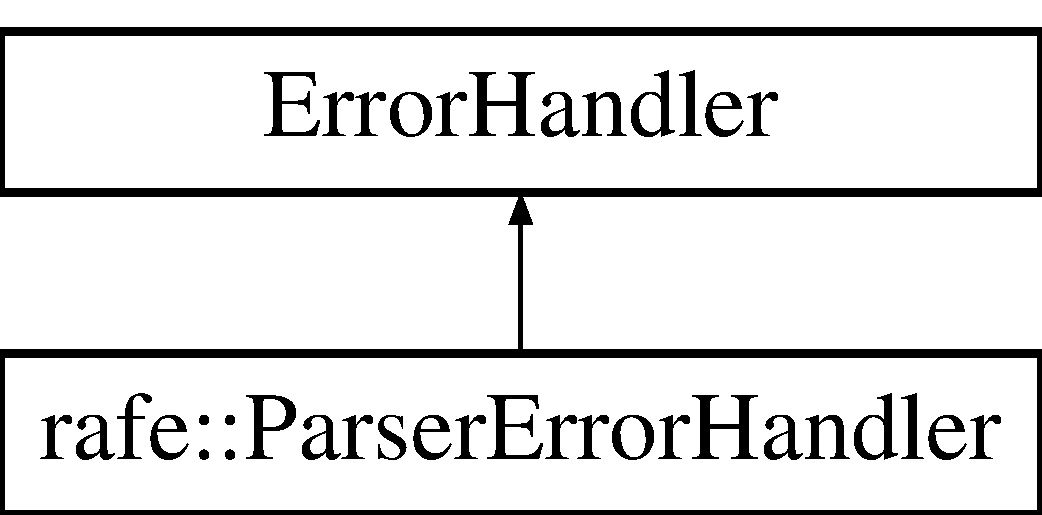
\includegraphics[height=2.000000cm]{classrafe_1_1_parser_error_handler}
\end{center}
\end{figure}
\subsection*{Public Member Functions}
\begin{DoxyCompactItemize}
\item 
\hyperlink{classrafe_1_1_parser_error_handler_a875a6ac56b59145378d4b2685f84ecb9}{Parser\+Error\+Handler} ()
\item 
void \hyperlink{classrafe_1_1_parser_error_handler_ab9807d119bb60ca2252ccdeac17637b8}{report\+Parse\+Exception} (const S\+A\+X\+Parse\+Exception \&ex)
\item 
void \hyperlink{classrafe_1_1_parser_error_handler_ab14d4e9a800f22af2698f13a3801a280}{warning} (const S\+A\+X\+Parse\+Exception \&ex)
\item 
void \hyperlink{classrafe_1_1_parser_error_handler_a974066afd1bef8087e80b4f075b7f0c2}{error} (const S\+A\+X\+Parse\+Exception \&ex)
\item 
void \hyperlink{classrafe_1_1_parser_error_handler_a55b044feacb8f734c08509be5d02c29d}{fatal\+Error} (const S\+A\+X\+Parse\+Exception \&ex)
\item 
void \hyperlink{classrafe_1_1_parser_error_handler_a02398bf9ec9b0bb9e772b5ffed1a3cdb}{reset\+Errors} ()
\end{DoxyCompactItemize}
\subsection*{Public Attributes}
\begin{DoxyCompactItemize}
\item 
int \hyperlink{classrafe_1_1_parser_error_handler_aee43a1438f6c79430cad5776220938ce}{errors}
\end{DoxyCompactItemize}


\subsection{Detailed Description}
Doma parser error handler. 

\subsection{Constructor \& Destructor Documentation}
\hypertarget{classrafe_1_1_parser_error_handler_a875a6ac56b59145378d4b2685f84ecb9}{\index{rafe\+::\+Parser\+Error\+Handler@{rafe\+::\+Parser\+Error\+Handler}!Parser\+Error\+Handler@{Parser\+Error\+Handler}}
\index{Parser\+Error\+Handler@{Parser\+Error\+Handler}!rafe\+::\+Parser\+Error\+Handler@{rafe\+::\+Parser\+Error\+Handler}}
\subsubsection[{Parser\+Error\+Handler}]{\setlength{\rightskip}{0pt plus 5cm}rafe\+::\+Parser\+Error\+Handler\+::\+Parser\+Error\+Handler (
\begin{DoxyParamCaption}
{}
\end{DoxyParamCaption}
)}}\label{classrafe_1_1_parser_error_handler_a875a6ac56b59145378d4b2685f84ecb9}
Creates new instance of \hyperlink{classrafe_1_1_parser_error_handler}{Parser\+Error\+Handler}. 

\subsection{Member Function Documentation}
\hypertarget{classrafe_1_1_parser_error_handler_a974066afd1bef8087e80b4f075b7f0c2}{\index{rafe\+::\+Parser\+Error\+Handler@{rafe\+::\+Parser\+Error\+Handler}!error@{error}}
\index{error@{error}!rafe\+::\+Parser\+Error\+Handler@{rafe\+::\+Parser\+Error\+Handler}}
\subsubsection[{error}]{\setlength{\rightskip}{0pt plus 5cm}void rafe\+::\+Parser\+Error\+Handler\+::error (
\begin{DoxyParamCaption}
\item[{const S\+A\+X\+Parse\+Exception \&}]{ex}
\end{DoxyParamCaption}
)}}\label{classrafe_1_1_parser_error_handler_a974066afd1bef8087e80b4f075b7f0c2}
Reports error. 
\begin{DoxyParams}{Parameters}
{\em ex} & -\/ reported error. \\
\hline
\end{DoxyParams}
\hypertarget{classrafe_1_1_parser_error_handler_a55b044feacb8f734c08509be5d02c29d}{\index{rafe\+::\+Parser\+Error\+Handler@{rafe\+::\+Parser\+Error\+Handler}!fatal\+Error@{fatal\+Error}}
\index{fatal\+Error@{fatal\+Error}!rafe\+::\+Parser\+Error\+Handler@{rafe\+::\+Parser\+Error\+Handler}}
\subsubsection[{fatal\+Error}]{\setlength{\rightskip}{0pt plus 5cm}void rafe\+::\+Parser\+Error\+Handler\+::fatal\+Error (
\begin{DoxyParamCaption}
\item[{const S\+A\+X\+Parse\+Exception \&}]{ex}
\end{DoxyParamCaption}
)}}\label{classrafe_1_1_parser_error_handler_a55b044feacb8f734c08509be5d02c29d}
Reports fatal error. 
\begin{DoxyParams}{Parameters}
{\em ex} & -\/ reported error. \\
\hline
\end{DoxyParams}
\hypertarget{classrafe_1_1_parser_error_handler_ab9807d119bb60ca2252ccdeac17637b8}{\index{rafe\+::\+Parser\+Error\+Handler@{rafe\+::\+Parser\+Error\+Handler}!report\+Parse\+Exception@{report\+Parse\+Exception}}
\index{report\+Parse\+Exception@{report\+Parse\+Exception}!rafe\+::\+Parser\+Error\+Handler@{rafe\+::\+Parser\+Error\+Handler}}
\subsubsection[{report\+Parse\+Exception}]{\setlength{\rightskip}{0pt plus 5cm}void rafe\+::\+Parser\+Error\+Handler\+::report\+Parse\+Exception (
\begin{DoxyParamCaption}
\item[{const S\+A\+X\+Parse\+Exception \&}]{ex}
\end{DoxyParamCaption}
)}}\label{classrafe_1_1_parser_error_handler_ab9807d119bb60ca2252ccdeac17637b8}
Reports S\+A\+X\+Parse\+Exception. 
\begin{DoxyParams}{Parameters}
{\em ex} & -\/ reported exception \\
\hline
\end{DoxyParams}
\hypertarget{classrafe_1_1_parser_error_handler_a02398bf9ec9b0bb9e772b5ffed1a3cdb}{\index{rafe\+::\+Parser\+Error\+Handler@{rafe\+::\+Parser\+Error\+Handler}!reset\+Errors@{reset\+Errors}}
\index{reset\+Errors@{reset\+Errors}!rafe\+::\+Parser\+Error\+Handler@{rafe\+::\+Parser\+Error\+Handler}}
\subsubsection[{reset\+Errors}]{\setlength{\rightskip}{0pt plus 5cm}void rafe\+::\+Parser\+Error\+Handler\+::reset\+Errors (
\begin{DoxyParamCaption}
{}
\end{DoxyParamCaption}
)}}\label{classrafe_1_1_parser_error_handler_a02398bf9ec9b0bb9e772b5ffed1a3cdb}
Resets reported errors. \hypertarget{classrafe_1_1_parser_error_handler_ab14d4e9a800f22af2698f13a3801a280}{\index{rafe\+::\+Parser\+Error\+Handler@{rafe\+::\+Parser\+Error\+Handler}!warning@{warning}}
\index{warning@{warning}!rafe\+::\+Parser\+Error\+Handler@{rafe\+::\+Parser\+Error\+Handler}}
\subsubsection[{warning}]{\setlength{\rightskip}{0pt plus 5cm}void rafe\+::\+Parser\+Error\+Handler\+::warning (
\begin{DoxyParamCaption}
\item[{const S\+A\+X\+Parse\+Exception \&}]{ex}
\end{DoxyParamCaption}
)}}\label{classrafe_1_1_parser_error_handler_ab14d4e9a800f22af2698f13a3801a280}
Reports warning. 
\begin{DoxyParams}{Parameters}
{\em ex} & -\/ reported warning. \\
\hline
\end{DoxyParams}


\subsection{Member Data Documentation}
\hypertarget{classrafe_1_1_parser_error_handler_aee43a1438f6c79430cad5776220938ce}{\index{rafe\+::\+Parser\+Error\+Handler@{rafe\+::\+Parser\+Error\+Handler}!errors@{errors}}
\index{errors@{errors}!rafe\+::\+Parser\+Error\+Handler@{rafe\+::\+Parser\+Error\+Handler}}
\subsubsection[{errors}]{\setlength{\rightskip}{0pt plus 5cm}int rafe\+::\+Parser\+Error\+Handler\+::errors}}\label{classrafe_1_1_parser_error_handler_aee43a1438f6c79430cad5776220938ce}
Stores number of errors. 

The documentation for this class was generated from the following files\+:\begin{DoxyCompactItemize}
\item 
C\+:/\+Users/\+Marcel/\+Documents/\+Visual Studio 2012/\+Projects/\+Relational\+Query\+Evaluator/\+Relational\+Query\+Evaluator/Xml\+Handler.\+h\item 
C\+:/\+Users/\+Marcel/\+Documents/\+Visual Studio 2012/\+Projects/\+Relational\+Query\+Evaluator/\+Relational\+Query\+Evaluator/Xml\+Handler.\+cpp\end{DoxyCompactItemize}

\hypertarget{classrafe_1_1_physical_operator}{\section{rafe\+:\+:Physical\+Operator Class Reference}
\label{classrafe_1_1_physical_operator}\index{rafe\+::\+Physical\+Operator@{rafe\+::\+Physical\+Operator}}
}


{\ttfamily \#include $<$Physical\+Operator.\+h$>$}

Inheritance diagram for rafe\+:\+:Physical\+Operator\+:\begin{figure}[H]
\begin{center}
\leavevmode
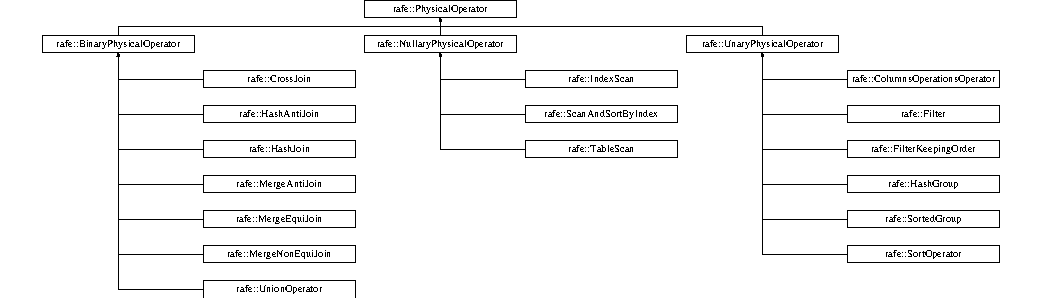
\includegraphics[height=4.000000cm]{classrafe_1_1_physical_operator}
\end{center}
\end{figure}
\subsection*{Public Member Functions}
\begin{DoxyCompactItemize}
\item 
virtual void \hyperlink{classrafe_1_1_physical_operator_a263a89f54604263cea897c5adf8944a3}{accept} (\hyperlink{classrafe_1_1_physical_operator_visitor}{Physical\+Operator\+Visitor} \&v)=0
\end{DoxyCompactItemize}
\subsection*{Public Attributes}
\begin{DoxyCompactItemize}
\item 
double \hyperlink{classrafe_1_1_physical_operator_a7b1bec2ef31be7b9c85ab32f543e23af}{time\+Complexity}
\item 
double \hyperlink{classrafe_1_1_physical_operator_a91df60e6935353504d02b9534a16eb4c}{size}
\item 
std\+::map$<$ int, \hyperlink{classrafe_1_1_column_info}{Column\+Info} $>$ \hyperlink{classrafe_1_1_physical_operator_a4056113435af85657e5b61d397db5165}{columns}
\end{DoxyCompactItemize}


\subsection{Detailed Description}
Base class for physical algorithms. 

\subsection{Member Function Documentation}
\hypertarget{classrafe_1_1_physical_operator_a263a89f54604263cea897c5adf8944a3}{\index{rafe\+::\+Physical\+Operator@{rafe\+::\+Physical\+Operator}!accept@{accept}}
\index{accept@{accept}!rafe\+::\+Physical\+Operator@{rafe\+::\+Physical\+Operator}}
\subsubsection[{accept}]{\setlength{\rightskip}{0pt plus 5cm}virtual void rafe\+::\+Physical\+Operator\+::accept (
\begin{DoxyParamCaption}
\item[{{\bf Physical\+Operator\+Visitor} \&}]{v}
\end{DoxyParamCaption}
)\hspace{0.3cm}{\ttfamily [pure virtual]}}}\label{classrafe_1_1_physical_operator_a263a89f54604263cea897c5adf8944a3}
Method for calling visit\mbox{[}node\mbox{]} on given \hyperlink{classrafe_1_1_physical_operator_visitor}{Physical\+Operator\+Visitor}. 
\begin{DoxyParams}{Parameters}
{\em v} & \hyperlink{classrafe_1_1_physical_operator_visitor}{Physical\+Operator\+Visitor}, on which to call function. \\
\hline
\end{DoxyParams}


Implemented in \hyperlink{classrafe_1_1_index_scan_a5e4e26317258097176b3b3b241653302}{rafe\+::\+Index\+Scan}, \hyperlink{classrafe_1_1_table_scan_a87cd9f9b093f153bd95b39bc3ea18678}{rafe\+::\+Table\+Scan}, \hyperlink{classrafe_1_1_scan_and_sort_by_index_aabb5d931b679a14bde40a1928ac10a52}{rafe\+::\+Scan\+And\+Sort\+By\+Index}, \hyperlink{classrafe_1_1_columns_operations_operator_a4fd8d03b5fd03393ea72dd46f4c11504}{rafe\+::\+Columns\+Operations\+Operator}, \hyperlink{classrafe_1_1_sorted_group_a2b9f2fbbe54f301a7b54050a67e1a4a2}{rafe\+::\+Sorted\+Group}, \hyperlink{classrafe_1_1_hash_group_a91335ef36a07f6ab099785073e16786b}{rafe\+::\+Hash\+Group}, \hyperlink{classrafe_1_1_union_operator_a5ae4b5f486376c816b10a81adbe784c7}{rafe\+::\+Union\+Operator}, \hyperlink{classrafe_1_1_merge_anti_join_aae93ebacaaed68ab8af8f38a09cfe8e7}{rafe\+::\+Merge\+Anti\+Join}, \hyperlink{classrafe_1_1_hash_anti_join_a3df56df88dd2e9280d6243cba23b4ac4}{rafe\+::\+Hash\+Anti\+Join}, \hyperlink{classrafe_1_1_hash_join_abd86be090582ddf7e87ac7d3dd2f60a7}{rafe\+::\+Hash\+Join}, \hyperlink{classrafe_1_1_merge_equi_join_a612f15e10eb741126e282b605fef0921}{rafe\+::\+Merge\+Equi\+Join}, \hyperlink{classrafe_1_1_merge_non_equi_join_a3accb9ad7ae5851370152885c23c6048}{rafe\+::\+Merge\+Non\+Equi\+Join}, \hyperlink{classrafe_1_1_cross_join_a3d9272caf9e1f2394f0d384f2813258a}{rafe\+::\+Cross\+Join}, \hyperlink{classrafe_1_1_sort_operator_ad2d3e9864cd1876d417a66b220b8dcb6}{rafe\+::\+Sort\+Operator}, \hyperlink{classrafe_1_1_filter_keeping_order_afde88521596d848cde18c0468aeb6062}{rafe\+::\+Filter\+Keeping\+Order}, \hyperlink{classrafe_1_1_filter_a27d15fd98afe3c03f05f5a4c5846b2a6}{rafe\+::\+Filter}, \hyperlink{classrafe_1_1_binary_physical_operator_a58ce0a14b970b2c932254419877a2e0e}{rafe\+::\+Binary\+Physical\+Operator}, \hyperlink{classrafe_1_1_unary_physical_operator_a56a160698a78f8a0aa44e47e0804f45e}{rafe\+::\+Unary\+Physical\+Operator}, and \hyperlink{classrafe_1_1_nullary_physical_operator_a0810fc4b368521ebe847fa48fcdcf948}{rafe\+::\+Nullary\+Physical\+Operator}.



\subsection{Member Data Documentation}
\hypertarget{classrafe_1_1_physical_operator_a4056113435af85657e5b61d397db5165}{\index{rafe\+::\+Physical\+Operator@{rafe\+::\+Physical\+Operator}!columns@{columns}}
\index{columns@{columns}!rafe\+::\+Physical\+Operator@{rafe\+::\+Physical\+Operator}}
\subsubsection[{columns}]{\setlength{\rightskip}{0pt plus 5cm}std\+::map$<$int, {\bf Column\+Info}$>$ rafe\+::\+Physical\+Operator\+::columns}}\label{classrafe_1_1_physical_operator_a4056113435af85657e5b61d397db5165}
Stores information about output columns from this operator. \hypertarget{classrafe_1_1_physical_operator_a91df60e6935353504d02b9534a16eb4c}{\index{rafe\+::\+Physical\+Operator@{rafe\+::\+Physical\+Operator}!size@{size}}
\index{size@{size}!rafe\+::\+Physical\+Operator@{rafe\+::\+Physical\+Operator}}
\subsubsection[{size}]{\setlength{\rightskip}{0pt plus 5cm}double rafe\+::\+Physical\+Operator\+::size}}\label{classrafe_1_1_physical_operator_a91df60e6935353504d02b9534a16eb4c}
Stores size of output relation. \hypertarget{classrafe_1_1_physical_operator_a7b1bec2ef31be7b9c85ab32f543e23af}{\index{rafe\+::\+Physical\+Operator@{rafe\+::\+Physical\+Operator}!time\+Complexity@{time\+Complexity}}
\index{time\+Complexity@{time\+Complexity}!rafe\+::\+Physical\+Operator@{rafe\+::\+Physical\+Operator}}
\subsubsection[{time\+Complexity}]{\setlength{\rightskip}{0pt plus 5cm}double rafe\+::\+Physical\+Operator\+::time\+Complexity}}\label{classrafe_1_1_physical_operator_a7b1bec2ef31be7b9c85ab32f543e23af}
Stores estimated run time of the operator. 

The documentation for this class was generated from the following file\+:\begin{DoxyCompactItemize}
\item 
C\+:/\+Users/\+Marcel/\+Documents/\+Visual Studio 2012/\+Projects/\+Relational\+Query\+Evaluator/\+Relational\+Query\+Evaluator/Physical\+Operator.\+h\end{DoxyCompactItemize}

\hypertarget{classrafe_1_1_physical_operator_drawing_visitor}{\section{rafe\+:\+:Physical\+Operator\+Drawing\+Visitor Class Reference}
\label{classrafe_1_1_physical_operator_drawing_visitor}\index{rafe\+::\+Physical\+Operator\+Drawing\+Visitor@{rafe\+::\+Physical\+Operator\+Drawing\+Visitor}}
}


{\ttfamily \#include $<$Physical\+Operator\+Visitor.\+h$>$}

Inheritance diagram for rafe\+:\+:Physical\+Operator\+Drawing\+Visitor\+:\begin{figure}[H]
\begin{center}
\leavevmode
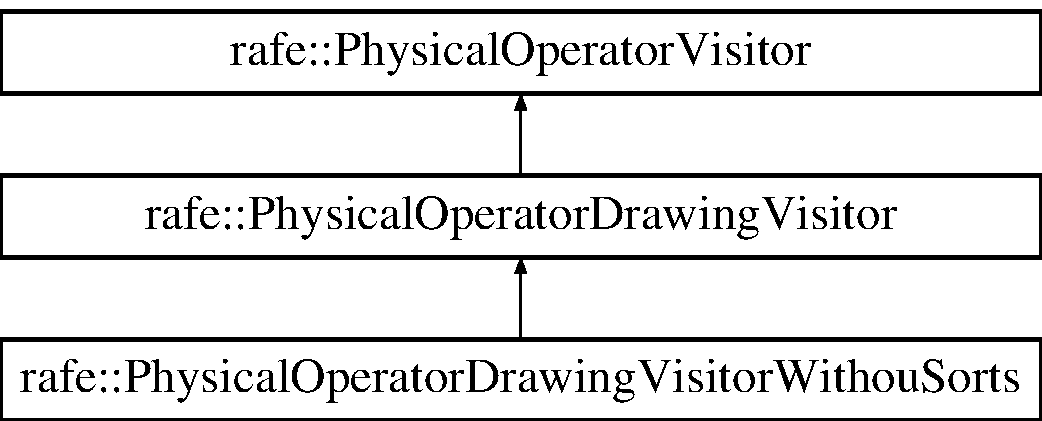
\includegraphics[height=3.000000cm]{classrafe_1_1_physical_operator_drawing_visitor}
\end{center}
\end{figure}
\subsection*{Public Member Functions}
\begin{DoxyCompactItemize}
\item 
\hyperlink{classrafe_1_1_physical_operator_drawing_visitor_a96e750b0d2c319d48c826843d67c9922}{Physical\+Operator\+Drawing\+Visitor} ()
\item 
void \hyperlink{classrafe_1_1_physical_operator_drawing_visitor_a8c34db1b84ad6fb8c8de4b5a27542062}{visit\+Filter} (\hyperlink{classrafe_1_1_filter}{Filter} $\ast$node)
\item 
void \hyperlink{classrafe_1_1_physical_operator_drawing_visitor_ad354fa6a9a6b139e893e4827ff2ecf3d}{visit\+Filter\+Keeping\+Order} (\hyperlink{classrafe_1_1_filter_keeping_order}{Filter\+Keeping\+Order} $\ast$node)
\item 
void \hyperlink{classrafe_1_1_physical_operator_drawing_visitor_a1d9f4efce36cd996b4d969e12f926560}{visit\+Sort\+Operator} (\hyperlink{classrafe_1_1_sort_operator}{Sort\+Operator} $\ast$node)
\item 
void \hyperlink{classrafe_1_1_physical_operator_drawing_visitor_aaa61a390184345f77b3d7d731f5eb042}{visit\+Merge\+Equi\+Join} (\hyperlink{classrafe_1_1_merge_equi_join}{Merge\+Equi\+Join} $\ast$node)
\item 
void \hyperlink{classrafe_1_1_physical_operator_drawing_visitor_ade0f29c6899eddf9fca59013eb079ac3}{visit\+Merge\+Non\+Equi\+Join} (\hyperlink{classrafe_1_1_merge_non_equi_join}{Merge\+Non\+Equi\+Join} $\ast$node)
\item 
void \hyperlink{classrafe_1_1_physical_operator_drawing_visitor_ae10d5b2b254263a0a206ba8056799746}{visit\+Cross\+Join} (\hyperlink{classrafe_1_1_cross_join}{Cross\+Join} $\ast$node)
\item 
void \hyperlink{classrafe_1_1_physical_operator_drawing_visitor_ac4be6a3ffbb85fd1d7a7f5ec109277ca}{visit\+Hash\+Join} (\hyperlink{classrafe_1_1_hash_join}{Hash\+Join} $\ast$node)
\item 
void \hyperlink{classrafe_1_1_physical_operator_drawing_visitor_aaff4651c152fd3d86805014459f5f565}{visit\+Hash\+Anti\+Join} (\hyperlink{classrafe_1_1_hash_anti_join}{Hash\+Anti\+Join} $\ast$node)
\item 
void \hyperlink{classrafe_1_1_physical_operator_drawing_visitor_a048897346f3a1344cab951f3d3ef7394}{visit\+Merge\+Anti\+Join} (\hyperlink{classrafe_1_1_merge_anti_join}{Merge\+Anti\+Join} $\ast$node)
\item 
void \hyperlink{classrafe_1_1_physical_operator_drawing_visitor_a9d9921709b02d719159ea0990f041ddd}{visit\+Union\+Operator} (\hyperlink{classrafe_1_1_union_operator}{Union\+Operator} $\ast$node)
\item 
void \hyperlink{classrafe_1_1_physical_operator_drawing_visitor_a81ede5f72bee22e9885236c8056a4556}{visit\+Hash\+Group} (\hyperlink{classrafe_1_1_hash_group}{Hash\+Group} $\ast$node)
\item 
void \hyperlink{classrafe_1_1_physical_operator_drawing_visitor_a5df8d5fca216ef12f6d9b836a310797f}{visit\+Sorted\+Group} (\hyperlink{classrafe_1_1_sorted_group}{Sorted\+Group} $\ast$node)
\item 
void \hyperlink{classrafe_1_1_physical_operator_drawing_visitor_a9c12b247be5746314eb74747bc5d50af}{visit\+Columns\+Operations\+Operator} (\hyperlink{classrafe_1_1_columns_operations_operator}{Columns\+Operations\+Operator} $\ast$node)
\item 
void \hyperlink{classrafe_1_1_physical_operator_drawing_visitor_abd677a519edaf4df41a7a32c7e0fd0cf}{visit\+Scan\+And\+Sort\+By\+Index} (\hyperlink{classrafe_1_1_scan_and_sort_by_index}{Scan\+And\+Sort\+By\+Index} $\ast$node)
\item 
void \hyperlink{classrafe_1_1_physical_operator_drawing_visitor_a0c61159c63401e8a96645a277459650e}{visit\+Table\+Scan} (\hyperlink{classrafe_1_1_table_scan}{Table\+Scan} $\ast$node)
\item 
void \hyperlink{classrafe_1_1_physical_operator_drawing_visitor_a6a74e5a271b3ab7ed954a2821f7dbcc9}{visit\+Index\+Scan} (\hyperlink{classrafe_1_1_index_scan}{Index\+Scan} $\ast$node)
\end{DoxyCompactItemize}
\subsection*{Public Attributes}
\begin{DoxyCompactItemize}
\item 
std\+::string \hyperlink{classrafe_1_1_physical_operator_drawing_visitor_a1e0b2d80743e6a11b4a75af0f68157d8}{result}
\item 
ulong \hyperlink{classrafe_1_1_physical_operator_drawing_visitor_a657ec262f628b93a56bb9ed016d02568}{node\+Counter}
\end{DoxyCompactItemize}


\subsection{Detailed Description}
Vsitor generates serialize physical tree to dot code. 

\subsection{Constructor \& Destructor Documentation}
\hypertarget{classrafe_1_1_physical_operator_drawing_visitor_a96e750b0d2c319d48c826843d67c9922}{\index{rafe\+::\+Physical\+Operator\+Drawing\+Visitor@{rafe\+::\+Physical\+Operator\+Drawing\+Visitor}!Physical\+Operator\+Drawing\+Visitor@{Physical\+Operator\+Drawing\+Visitor}}
\index{Physical\+Operator\+Drawing\+Visitor@{Physical\+Operator\+Drawing\+Visitor}!rafe\+::\+Physical\+Operator\+Drawing\+Visitor@{rafe\+::\+Physical\+Operator\+Drawing\+Visitor}}
\subsubsection[{Physical\+Operator\+Drawing\+Visitor}]{\setlength{\rightskip}{0pt plus 5cm}rafe\+::\+Physical\+Operator\+Drawing\+Visitor\+::\+Physical\+Operator\+Drawing\+Visitor (
\begin{DoxyParamCaption}
{}
\end{DoxyParamCaption}
)}}\label{classrafe_1_1_physical_operator_drawing_visitor_a96e750b0d2c319d48c826843d67c9922}
Creates new instance of \hyperlink{classrafe_1_1_physical_operator_drawing_visitor}{Physical\+Operator\+Drawing\+Visitor}. 

\subsection{Member Function Documentation}
\hypertarget{classrafe_1_1_physical_operator_drawing_visitor_a9c12b247be5746314eb74747bc5d50af}{\index{rafe\+::\+Physical\+Operator\+Drawing\+Visitor@{rafe\+::\+Physical\+Operator\+Drawing\+Visitor}!visit\+Columns\+Operations\+Operator@{visit\+Columns\+Operations\+Operator}}
\index{visit\+Columns\+Operations\+Operator@{visit\+Columns\+Operations\+Operator}!rafe\+::\+Physical\+Operator\+Drawing\+Visitor@{rafe\+::\+Physical\+Operator\+Drawing\+Visitor}}
\subsubsection[{visit\+Columns\+Operations\+Operator}]{\setlength{\rightskip}{0pt plus 5cm}void rafe\+::\+Physical\+Operator\+Drawing\+Visitor\+::visit\+Columns\+Operations\+Operator (
\begin{DoxyParamCaption}
\item[{{\bf Columns\+Operations\+Operator} $\ast$}]{node}
\end{DoxyParamCaption}
)\hspace{0.3cm}{\ttfamily [virtual]}}}\label{classrafe_1_1_physical_operator_drawing_visitor_a9c12b247be5746314eb74747bc5d50af}
Visits physical operator \hyperlink{classrafe_1_1_columns_operations_operator}{Columns\+Operations\+Operator}. 
\begin{DoxyParams}{Parameters}
{\em node} & visited \hyperlink{classrafe_1_1_columns_operations_operator}{Columns\+Operations\+Operator}. \\
\hline
\end{DoxyParams}


Reimplemented from \hyperlink{classrafe_1_1_physical_operator_visitor_ab69b85d7a2c8f89986d84cbcce6f2f89}{rafe\+::\+Physical\+Operator\+Visitor}.

\hypertarget{classrafe_1_1_physical_operator_drawing_visitor_ae10d5b2b254263a0a206ba8056799746}{\index{rafe\+::\+Physical\+Operator\+Drawing\+Visitor@{rafe\+::\+Physical\+Operator\+Drawing\+Visitor}!visit\+Cross\+Join@{visit\+Cross\+Join}}
\index{visit\+Cross\+Join@{visit\+Cross\+Join}!rafe\+::\+Physical\+Operator\+Drawing\+Visitor@{rafe\+::\+Physical\+Operator\+Drawing\+Visitor}}
\subsubsection[{visit\+Cross\+Join}]{\setlength{\rightskip}{0pt plus 5cm}void rafe\+::\+Physical\+Operator\+Drawing\+Visitor\+::visit\+Cross\+Join (
\begin{DoxyParamCaption}
\item[{{\bf Cross\+Join} $\ast$}]{node}
\end{DoxyParamCaption}
)\hspace{0.3cm}{\ttfamily [virtual]}}}\label{classrafe_1_1_physical_operator_drawing_visitor_ae10d5b2b254263a0a206ba8056799746}
Visits physical operator \hyperlink{classrafe_1_1_cross_join}{Cross\+Join}. 
\begin{DoxyParams}{Parameters}
{\em node} & visited \hyperlink{classrafe_1_1_cross_join}{Cross\+Join}. \\
\hline
\end{DoxyParams}


Reimplemented from \hyperlink{classrafe_1_1_physical_operator_visitor_acc39509ae79aa6848ec928cc4f616d61}{rafe\+::\+Physical\+Operator\+Visitor}.

\hypertarget{classrafe_1_1_physical_operator_drawing_visitor_a8c34db1b84ad6fb8c8de4b5a27542062}{\index{rafe\+::\+Physical\+Operator\+Drawing\+Visitor@{rafe\+::\+Physical\+Operator\+Drawing\+Visitor}!visit\+Filter@{visit\+Filter}}
\index{visit\+Filter@{visit\+Filter}!rafe\+::\+Physical\+Operator\+Drawing\+Visitor@{rafe\+::\+Physical\+Operator\+Drawing\+Visitor}}
\subsubsection[{visit\+Filter}]{\setlength{\rightskip}{0pt plus 5cm}void rafe\+::\+Physical\+Operator\+Drawing\+Visitor\+::visit\+Filter (
\begin{DoxyParamCaption}
\item[{{\bf Filter} $\ast$}]{node}
\end{DoxyParamCaption}
)\hspace{0.3cm}{\ttfamily [virtual]}}}\label{classrafe_1_1_physical_operator_drawing_visitor_a8c34db1b84ad6fb8c8de4b5a27542062}
Visits physical operator \hyperlink{classrafe_1_1_filter}{Filter}. 
\begin{DoxyParams}{Parameters}
{\em node} & visited \hyperlink{classrafe_1_1_filter}{Filter}. \\
\hline
\end{DoxyParams}


Reimplemented from \hyperlink{classrafe_1_1_physical_operator_visitor_a516a84d305910f3e1b9d1ae2cb184b24}{rafe\+::\+Physical\+Operator\+Visitor}.

\hypertarget{classrafe_1_1_physical_operator_drawing_visitor_ad354fa6a9a6b139e893e4827ff2ecf3d}{\index{rafe\+::\+Physical\+Operator\+Drawing\+Visitor@{rafe\+::\+Physical\+Operator\+Drawing\+Visitor}!visit\+Filter\+Keeping\+Order@{visit\+Filter\+Keeping\+Order}}
\index{visit\+Filter\+Keeping\+Order@{visit\+Filter\+Keeping\+Order}!rafe\+::\+Physical\+Operator\+Drawing\+Visitor@{rafe\+::\+Physical\+Operator\+Drawing\+Visitor}}
\subsubsection[{visit\+Filter\+Keeping\+Order}]{\setlength{\rightskip}{0pt plus 5cm}void rafe\+::\+Physical\+Operator\+Drawing\+Visitor\+::visit\+Filter\+Keeping\+Order (
\begin{DoxyParamCaption}
\item[{{\bf Filter\+Keeping\+Order} $\ast$}]{node}
\end{DoxyParamCaption}
)\hspace{0.3cm}{\ttfamily [virtual]}}}\label{classrafe_1_1_physical_operator_drawing_visitor_ad354fa6a9a6b139e893e4827ff2ecf3d}
Visits physical operator \hyperlink{classrafe_1_1_filter_keeping_order}{Filter\+Keeping\+Order}. 
\begin{DoxyParams}{Parameters}
{\em node} & visited \hyperlink{classrafe_1_1_filter_keeping_order}{Filter\+Keeping\+Order}. \\
\hline
\end{DoxyParams}


Reimplemented from \hyperlink{classrafe_1_1_physical_operator_visitor_a7b581054d167c71fa5443570a6808740}{rafe\+::\+Physical\+Operator\+Visitor}.

\hypertarget{classrafe_1_1_physical_operator_drawing_visitor_aaff4651c152fd3d86805014459f5f565}{\index{rafe\+::\+Physical\+Operator\+Drawing\+Visitor@{rafe\+::\+Physical\+Operator\+Drawing\+Visitor}!visit\+Hash\+Anti\+Join@{visit\+Hash\+Anti\+Join}}
\index{visit\+Hash\+Anti\+Join@{visit\+Hash\+Anti\+Join}!rafe\+::\+Physical\+Operator\+Drawing\+Visitor@{rafe\+::\+Physical\+Operator\+Drawing\+Visitor}}
\subsubsection[{visit\+Hash\+Anti\+Join}]{\setlength{\rightskip}{0pt plus 5cm}void rafe\+::\+Physical\+Operator\+Drawing\+Visitor\+::visit\+Hash\+Anti\+Join (
\begin{DoxyParamCaption}
\item[{{\bf Hash\+Anti\+Join} $\ast$}]{node}
\end{DoxyParamCaption}
)\hspace{0.3cm}{\ttfamily [virtual]}}}\label{classrafe_1_1_physical_operator_drawing_visitor_aaff4651c152fd3d86805014459f5f565}
Visits physical operator \hyperlink{classrafe_1_1_hash_anti_join}{Hash\+Anti\+Join}. 
\begin{DoxyParams}{Parameters}
{\em node} & visited \hyperlink{classrafe_1_1_hash_anti_join}{Hash\+Anti\+Join}. \\
\hline
\end{DoxyParams}


Reimplemented from \hyperlink{classrafe_1_1_physical_operator_visitor_a9415b5939da4948ac922e63fbece1135}{rafe\+::\+Physical\+Operator\+Visitor}.

\hypertarget{classrafe_1_1_physical_operator_drawing_visitor_a81ede5f72bee22e9885236c8056a4556}{\index{rafe\+::\+Physical\+Operator\+Drawing\+Visitor@{rafe\+::\+Physical\+Operator\+Drawing\+Visitor}!visit\+Hash\+Group@{visit\+Hash\+Group}}
\index{visit\+Hash\+Group@{visit\+Hash\+Group}!rafe\+::\+Physical\+Operator\+Drawing\+Visitor@{rafe\+::\+Physical\+Operator\+Drawing\+Visitor}}
\subsubsection[{visit\+Hash\+Group}]{\setlength{\rightskip}{0pt plus 5cm}void rafe\+::\+Physical\+Operator\+Drawing\+Visitor\+::visit\+Hash\+Group (
\begin{DoxyParamCaption}
\item[{{\bf Hash\+Group} $\ast$}]{node}
\end{DoxyParamCaption}
)\hspace{0.3cm}{\ttfamily [virtual]}}}\label{classrafe_1_1_physical_operator_drawing_visitor_a81ede5f72bee22e9885236c8056a4556}
Visits physical operator \hyperlink{classrafe_1_1_hash_group}{Hash\+Group}. 
\begin{DoxyParams}{Parameters}
{\em node} & visited \hyperlink{classrafe_1_1_hash_group}{Hash\+Group}. \\
\hline
\end{DoxyParams}


Reimplemented from \hyperlink{classrafe_1_1_physical_operator_visitor_ab6a2b2b02f2237fd41e6c44f5b2ede9b}{rafe\+::\+Physical\+Operator\+Visitor}.

\hypertarget{classrafe_1_1_physical_operator_drawing_visitor_ac4be6a3ffbb85fd1d7a7f5ec109277ca}{\index{rafe\+::\+Physical\+Operator\+Drawing\+Visitor@{rafe\+::\+Physical\+Operator\+Drawing\+Visitor}!visit\+Hash\+Join@{visit\+Hash\+Join}}
\index{visit\+Hash\+Join@{visit\+Hash\+Join}!rafe\+::\+Physical\+Operator\+Drawing\+Visitor@{rafe\+::\+Physical\+Operator\+Drawing\+Visitor}}
\subsubsection[{visit\+Hash\+Join}]{\setlength{\rightskip}{0pt plus 5cm}void rafe\+::\+Physical\+Operator\+Drawing\+Visitor\+::visit\+Hash\+Join (
\begin{DoxyParamCaption}
\item[{{\bf Hash\+Join} $\ast$}]{node}
\end{DoxyParamCaption}
)\hspace{0.3cm}{\ttfamily [virtual]}}}\label{classrafe_1_1_physical_operator_drawing_visitor_ac4be6a3ffbb85fd1d7a7f5ec109277ca}
Visits physical operator \hyperlink{classrafe_1_1_hash_join}{Hash\+Join}. 
\begin{DoxyParams}{Parameters}
{\em node} & visited \hyperlink{classrafe_1_1_hash_join}{Hash\+Join}. \\
\hline
\end{DoxyParams}


Reimplemented from \hyperlink{classrafe_1_1_physical_operator_visitor_ae36c9ef817768f134d35fe5b3834855c}{rafe\+::\+Physical\+Operator\+Visitor}.

\hypertarget{classrafe_1_1_physical_operator_drawing_visitor_a6a74e5a271b3ab7ed954a2821f7dbcc9}{\index{rafe\+::\+Physical\+Operator\+Drawing\+Visitor@{rafe\+::\+Physical\+Operator\+Drawing\+Visitor}!visit\+Index\+Scan@{visit\+Index\+Scan}}
\index{visit\+Index\+Scan@{visit\+Index\+Scan}!rafe\+::\+Physical\+Operator\+Drawing\+Visitor@{rafe\+::\+Physical\+Operator\+Drawing\+Visitor}}
\subsubsection[{visit\+Index\+Scan}]{\setlength{\rightskip}{0pt plus 5cm}void rafe\+::\+Physical\+Operator\+Drawing\+Visitor\+::visit\+Index\+Scan (
\begin{DoxyParamCaption}
\item[{{\bf Index\+Scan} $\ast$}]{node}
\end{DoxyParamCaption}
)\hspace{0.3cm}{\ttfamily [virtual]}}}\label{classrafe_1_1_physical_operator_drawing_visitor_a6a74e5a271b3ab7ed954a2821f7dbcc9}
Visits physical operator \hyperlink{classrafe_1_1_index_scan}{Index\+Scan}. 
\begin{DoxyParams}{Parameters}
{\em node} & visited \hyperlink{classrafe_1_1_index_scan}{Index\+Scan}. \\
\hline
\end{DoxyParams}


Reimplemented from \hyperlink{classrafe_1_1_physical_operator_visitor_ac33ea100cdb3e642a58a82c4367de3fd}{rafe\+::\+Physical\+Operator\+Visitor}.

\hypertarget{classrafe_1_1_physical_operator_drawing_visitor_a048897346f3a1344cab951f3d3ef7394}{\index{rafe\+::\+Physical\+Operator\+Drawing\+Visitor@{rafe\+::\+Physical\+Operator\+Drawing\+Visitor}!visit\+Merge\+Anti\+Join@{visit\+Merge\+Anti\+Join}}
\index{visit\+Merge\+Anti\+Join@{visit\+Merge\+Anti\+Join}!rafe\+::\+Physical\+Operator\+Drawing\+Visitor@{rafe\+::\+Physical\+Operator\+Drawing\+Visitor}}
\subsubsection[{visit\+Merge\+Anti\+Join}]{\setlength{\rightskip}{0pt plus 5cm}void rafe\+::\+Physical\+Operator\+Drawing\+Visitor\+::visit\+Merge\+Anti\+Join (
\begin{DoxyParamCaption}
\item[{{\bf Merge\+Anti\+Join} $\ast$}]{node}
\end{DoxyParamCaption}
)\hspace{0.3cm}{\ttfamily [virtual]}}}\label{classrafe_1_1_physical_operator_drawing_visitor_a048897346f3a1344cab951f3d3ef7394}
Visits physical operator \hyperlink{classrafe_1_1_merge_anti_join}{Merge\+Anti\+Join}. 
\begin{DoxyParams}{Parameters}
{\em node} & visited \hyperlink{classrafe_1_1_merge_anti_join}{Merge\+Anti\+Join}. \\
\hline
\end{DoxyParams}


Reimplemented from \hyperlink{classrafe_1_1_physical_operator_visitor_a0f3496aaac992756bbb8f18c1000ed75}{rafe\+::\+Physical\+Operator\+Visitor}.

\hypertarget{classrafe_1_1_physical_operator_drawing_visitor_aaa61a390184345f77b3d7d731f5eb042}{\index{rafe\+::\+Physical\+Operator\+Drawing\+Visitor@{rafe\+::\+Physical\+Operator\+Drawing\+Visitor}!visit\+Merge\+Equi\+Join@{visit\+Merge\+Equi\+Join}}
\index{visit\+Merge\+Equi\+Join@{visit\+Merge\+Equi\+Join}!rafe\+::\+Physical\+Operator\+Drawing\+Visitor@{rafe\+::\+Physical\+Operator\+Drawing\+Visitor}}
\subsubsection[{visit\+Merge\+Equi\+Join}]{\setlength{\rightskip}{0pt plus 5cm}void rafe\+::\+Physical\+Operator\+Drawing\+Visitor\+::visit\+Merge\+Equi\+Join (
\begin{DoxyParamCaption}
\item[{{\bf Merge\+Equi\+Join} $\ast$}]{node}
\end{DoxyParamCaption}
)\hspace{0.3cm}{\ttfamily [virtual]}}}\label{classrafe_1_1_physical_operator_drawing_visitor_aaa61a390184345f77b3d7d731f5eb042}
Visits physical operator \hyperlink{classrafe_1_1_merge_equi_join}{Merge\+Equi\+Join}. 
\begin{DoxyParams}{Parameters}
{\em node} & visited \hyperlink{classrafe_1_1_merge_equi_join}{Merge\+Equi\+Join}. \\
\hline
\end{DoxyParams}


Reimplemented from \hyperlink{classrafe_1_1_physical_operator_visitor_a9fd16981e6fbb9b545b7edeaabcf97bf}{rafe\+::\+Physical\+Operator\+Visitor}.

\hypertarget{classrafe_1_1_physical_operator_drawing_visitor_ade0f29c6899eddf9fca59013eb079ac3}{\index{rafe\+::\+Physical\+Operator\+Drawing\+Visitor@{rafe\+::\+Physical\+Operator\+Drawing\+Visitor}!visit\+Merge\+Non\+Equi\+Join@{visit\+Merge\+Non\+Equi\+Join}}
\index{visit\+Merge\+Non\+Equi\+Join@{visit\+Merge\+Non\+Equi\+Join}!rafe\+::\+Physical\+Operator\+Drawing\+Visitor@{rafe\+::\+Physical\+Operator\+Drawing\+Visitor}}
\subsubsection[{visit\+Merge\+Non\+Equi\+Join}]{\setlength{\rightskip}{0pt plus 5cm}void rafe\+::\+Physical\+Operator\+Drawing\+Visitor\+::visit\+Merge\+Non\+Equi\+Join (
\begin{DoxyParamCaption}
\item[{{\bf Merge\+Non\+Equi\+Join} $\ast$}]{node}
\end{DoxyParamCaption}
)\hspace{0.3cm}{\ttfamily [virtual]}}}\label{classrafe_1_1_physical_operator_drawing_visitor_ade0f29c6899eddf9fca59013eb079ac3}
Visits physical operator \hyperlink{classrafe_1_1_merge_non_equi_join}{Merge\+Non\+Equi\+Join}. 
\begin{DoxyParams}{Parameters}
{\em node} & visited \hyperlink{classrafe_1_1_merge_non_equi_join}{Merge\+Non\+Equi\+Join}. \\
\hline
\end{DoxyParams}


Reimplemented from \hyperlink{classrafe_1_1_physical_operator_visitor_a1d4af9c73ece300d7a90c65481cd8e06}{rafe\+::\+Physical\+Operator\+Visitor}.

\hypertarget{classrafe_1_1_physical_operator_drawing_visitor_abd677a519edaf4df41a7a32c7e0fd0cf}{\index{rafe\+::\+Physical\+Operator\+Drawing\+Visitor@{rafe\+::\+Physical\+Operator\+Drawing\+Visitor}!visit\+Scan\+And\+Sort\+By\+Index@{visit\+Scan\+And\+Sort\+By\+Index}}
\index{visit\+Scan\+And\+Sort\+By\+Index@{visit\+Scan\+And\+Sort\+By\+Index}!rafe\+::\+Physical\+Operator\+Drawing\+Visitor@{rafe\+::\+Physical\+Operator\+Drawing\+Visitor}}
\subsubsection[{visit\+Scan\+And\+Sort\+By\+Index}]{\setlength{\rightskip}{0pt plus 5cm}void rafe\+::\+Physical\+Operator\+Drawing\+Visitor\+::visit\+Scan\+And\+Sort\+By\+Index (
\begin{DoxyParamCaption}
\item[{{\bf Scan\+And\+Sort\+By\+Index} $\ast$}]{node}
\end{DoxyParamCaption}
)\hspace{0.3cm}{\ttfamily [virtual]}}}\label{classrafe_1_1_physical_operator_drawing_visitor_abd677a519edaf4df41a7a32c7e0fd0cf}
Visits physical operator \hyperlink{classrafe_1_1_scan_and_sort_by_index}{Scan\+And\+Sort\+By\+Index}. 
\begin{DoxyParams}{Parameters}
{\em node} & visited \hyperlink{classrafe_1_1_scan_and_sort_by_index}{Scan\+And\+Sort\+By\+Index}. \\
\hline
\end{DoxyParams}


Reimplemented from \hyperlink{classrafe_1_1_physical_operator_visitor_a4f8cbef9d1c5a58fceb44deb4a7d998c}{rafe\+::\+Physical\+Operator\+Visitor}.

\hypertarget{classrafe_1_1_physical_operator_drawing_visitor_a5df8d5fca216ef12f6d9b836a310797f}{\index{rafe\+::\+Physical\+Operator\+Drawing\+Visitor@{rafe\+::\+Physical\+Operator\+Drawing\+Visitor}!visit\+Sorted\+Group@{visit\+Sorted\+Group}}
\index{visit\+Sorted\+Group@{visit\+Sorted\+Group}!rafe\+::\+Physical\+Operator\+Drawing\+Visitor@{rafe\+::\+Physical\+Operator\+Drawing\+Visitor}}
\subsubsection[{visit\+Sorted\+Group}]{\setlength{\rightskip}{0pt plus 5cm}void rafe\+::\+Physical\+Operator\+Drawing\+Visitor\+::visit\+Sorted\+Group (
\begin{DoxyParamCaption}
\item[{{\bf Sorted\+Group} $\ast$}]{node}
\end{DoxyParamCaption}
)\hspace{0.3cm}{\ttfamily [virtual]}}}\label{classrafe_1_1_physical_operator_drawing_visitor_a5df8d5fca216ef12f6d9b836a310797f}
Visits physical operator \hyperlink{classrafe_1_1_sorted_group}{Sorted\+Group}. 
\begin{DoxyParams}{Parameters}
{\em node} & visited \hyperlink{classrafe_1_1_sorted_group}{Sorted\+Group}. \\
\hline
\end{DoxyParams}


Reimplemented from \hyperlink{classrafe_1_1_physical_operator_visitor_afb1b6786bf12f12e3b1c2895bf77e874}{rafe\+::\+Physical\+Operator\+Visitor}.

\hypertarget{classrafe_1_1_physical_operator_drawing_visitor_a1d9f4efce36cd996b4d969e12f926560}{\index{rafe\+::\+Physical\+Operator\+Drawing\+Visitor@{rafe\+::\+Physical\+Operator\+Drawing\+Visitor}!visit\+Sort\+Operator@{visit\+Sort\+Operator}}
\index{visit\+Sort\+Operator@{visit\+Sort\+Operator}!rafe\+::\+Physical\+Operator\+Drawing\+Visitor@{rafe\+::\+Physical\+Operator\+Drawing\+Visitor}}
\subsubsection[{visit\+Sort\+Operator}]{\setlength{\rightskip}{0pt plus 5cm}void rafe\+::\+Physical\+Operator\+Drawing\+Visitor\+::visit\+Sort\+Operator (
\begin{DoxyParamCaption}
\item[{{\bf Sort\+Operator} $\ast$}]{node}
\end{DoxyParamCaption}
)\hspace{0.3cm}{\ttfamily [virtual]}}}\label{classrafe_1_1_physical_operator_drawing_visitor_a1d9f4efce36cd996b4d969e12f926560}
Visits physical operator \hyperlink{classrafe_1_1_sort_operator}{Sort\+Operator}. 
\begin{DoxyParams}{Parameters}
{\em node} & visited \hyperlink{classrafe_1_1_sort_operator}{Sort\+Operator}. \\
\hline
\end{DoxyParams}


Reimplemented from \hyperlink{classrafe_1_1_physical_operator_visitor_adaee48b1ef175226c860c7b2d70ba15d}{rafe\+::\+Physical\+Operator\+Visitor}.

\hypertarget{classrafe_1_1_physical_operator_drawing_visitor_a0c61159c63401e8a96645a277459650e}{\index{rafe\+::\+Physical\+Operator\+Drawing\+Visitor@{rafe\+::\+Physical\+Operator\+Drawing\+Visitor}!visit\+Table\+Scan@{visit\+Table\+Scan}}
\index{visit\+Table\+Scan@{visit\+Table\+Scan}!rafe\+::\+Physical\+Operator\+Drawing\+Visitor@{rafe\+::\+Physical\+Operator\+Drawing\+Visitor}}
\subsubsection[{visit\+Table\+Scan}]{\setlength{\rightskip}{0pt plus 5cm}void rafe\+::\+Physical\+Operator\+Drawing\+Visitor\+::visit\+Table\+Scan (
\begin{DoxyParamCaption}
\item[{{\bf Table\+Scan} $\ast$}]{node}
\end{DoxyParamCaption}
)\hspace{0.3cm}{\ttfamily [virtual]}}}\label{classrafe_1_1_physical_operator_drawing_visitor_a0c61159c63401e8a96645a277459650e}
Visits physical operator \hyperlink{classrafe_1_1_table_scan}{Table\+Scan}. 
\begin{DoxyParams}{Parameters}
{\em node} & visited \hyperlink{classrafe_1_1_table_scan}{Table\+Scan}. \\
\hline
\end{DoxyParams}


Reimplemented from \hyperlink{classrafe_1_1_physical_operator_visitor_ae3d5b2b56e9465713c5ecd4e5fcea9c9}{rafe\+::\+Physical\+Operator\+Visitor}.

\hypertarget{classrafe_1_1_physical_operator_drawing_visitor_a9d9921709b02d719159ea0990f041ddd}{\index{rafe\+::\+Physical\+Operator\+Drawing\+Visitor@{rafe\+::\+Physical\+Operator\+Drawing\+Visitor}!visit\+Union\+Operator@{visit\+Union\+Operator}}
\index{visit\+Union\+Operator@{visit\+Union\+Operator}!rafe\+::\+Physical\+Operator\+Drawing\+Visitor@{rafe\+::\+Physical\+Operator\+Drawing\+Visitor}}
\subsubsection[{visit\+Union\+Operator}]{\setlength{\rightskip}{0pt plus 5cm}void rafe\+::\+Physical\+Operator\+Drawing\+Visitor\+::visit\+Union\+Operator (
\begin{DoxyParamCaption}
\item[{{\bf Union\+Operator} $\ast$}]{node}
\end{DoxyParamCaption}
)\hspace{0.3cm}{\ttfamily [virtual]}}}\label{classrafe_1_1_physical_operator_drawing_visitor_a9d9921709b02d719159ea0990f041ddd}
Visits physical operator \hyperlink{classrafe_1_1_union_operator}{Union\+Operator}. 
\begin{DoxyParams}{Parameters}
{\em node} & visited \hyperlink{classrafe_1_1_union_operator}{Union\+Operator}. \\
\hline
\end{DoxyParams}


Reimplemented from \hyperlink{classrafe_1_1_physical_operator_visitor_a01eb10e07cc1fbe7622bc1eb01fa3b79}{rafe\+::\+Physical\+Operator\+Visitor}.



\subsection{Member Data Documentation}
\hypertarget{classrafe_1_1_physical_operator_drawing_visitor_a657ec262f628b93a56bb9ed016d02568}{\index{rafe\+::\+Physical\+Operator\+Drawing\+Visitor@{rafe\+::\+Physical\+Operator\+Drawing\+Visitor}!node\+Counter@{node\+Counter}}
\index{node\+Counter@{node\+Counter}!rafe\+::\+Physical\+Operator\+Drawing\+Visitor@{rafe\+::\+Physical\+Operator\+Drawing\+Visitor}}
\subsubsection[{node\+Counter}]{\setlength{\rightskip}{0pt plus 5cm}ulong rafe\+::\+Physical\+Operator\+Drawing\+Visitor\+::node\+Counter}}\label{classrafe_1_1_physical_operator_drawing_visitor_a657ec262f628b93a56bb9ed016d02568}
Variable that counts nodes. \hypertarget{classrafe_1_1_physical_operator_drawing_visitor_a1e0b2d80743e6a11b4a75af0f68157d8}{\index{rafe\+::\+Physical\+Operator\+Drawing\+Visitor@{rafe\+::\+Physical\+Operator\+Drawing\+Visitor}!result@{result}}
\index{result@{result}!rafe\+::\+Physical\+Operator\+Drawing\+Visitor@{rafe\+::\+Physical\+Operator\+Drawing\+Visitor}}
\subsubsection[{result}]{\setlength{\rightskip}{0pt plus 5cm}std\+::string rafe\+::\+Physical\+Operator\+Drawing\+Visitor\+::result}}\label{classrafe_1_1_physical_operator_drawing_visitor_a1e0b2d80743e6a11b4a75af0f68157d8}
Final dot representation. 

The documentation for this class was generated from the following files\+:\begin{DoxyCompactItemize}
\item 
C\+:/\+Users/\+Marcel/\+Documents/\+Visual Studio 2012/\+Projects/\+Relational\+Query\+Evaluator/\+Relational\+Query\+Evaluator/Physical\+Operator\+Visitor.\+h\item 
C\+:/\+Users/\+Marcel/\+Documents/\+Visual Studio 2012/\+Projects/\+Relational\+Query\+Evaluator/\+Relational\+Query\+Evaluator/Physical\+Operator\+Visitor.\+cpp\end{DoxyCompactItemize}

\hypertarget{classrafe_1_1_physical_operator_drawing_visitor_withou_sorts}{\section{rafe\+:\+:Physical\+Operator\+Drawing\+Visitor\+Withou\+Sorts Class Reference}
\label{classrafe_1_1_physical_operator_drawing_visitor_withou_sorts}\index{rafe\+::\+Physical\+Operator\+Drawing\+Visitor\+Withou\+Sorts@{rafe\+::\+Physical\+Operator\+Drawing\+Visitor\+Withou\+Sorts}}
}


{\ttfamily \#include $<$Physical\+Operator\+Visitor.\+h$>$}

Inheritance diagram for rafe\+:\+:Physical\+Operator\+Drawing\+Visitor\+Withou\+Sorts\+:\begin{figure}[H]
\begin{center}
\leavevmode
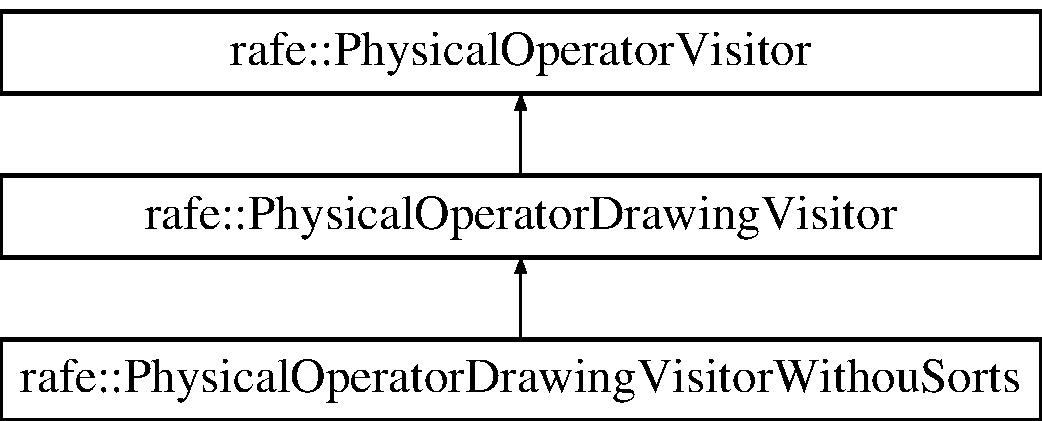
\includegraphics[height=3.000000cm]{classrafe_1_1_physical_operator_drawing_visitor_withou_sorts}
\end{center}
\end{figure}
\subsection*{Additional Inherited Members}


\subsection{Detailed Description}
Visitor generates physical tree to dot code. Visitor does the same as \hyperlink{classrafe_1_1_physical_operator_drawing_visitor}{Physical\+Operator\+Drawing\+Visitor}, except it does not write sorts, which output and input are sorted same size. 

The documentation for this class was generated from the following files\+:\begin{DoxyCompactItemize}
\item 
C\+:/\+Users/\+Marcel/\+Documents/\+Visual Studio 2012/\+Projects/\+Relational\+Query\+Evaluator/\+Relational\+Query\+Evaluator/Physical\+Operator\+Visitor.\+h\item 
C\+:/\+Users/\+Marcel/\+Documents/\+Visual Studio 2012/\+Projects/\+Relational\+Query\+Evaluator/\+Relational\+Query\+Evaluator/Physical\+Operator\+Visitor.\+cpp\end{DoxyCompactItemize}

\hypertarget{classrafe_1_1_physical_operator_visitor}{\section{rafe\+:\+:Physical\+Operator\+Visitor Class Reference}
\label{classrafe_1_1_physical_operator_visitor}\index{rafe\+::\+Physical\+Operator\+Visitor@{rafe\+::\+Physical\+Operator\+Visitor}}
}


{\ttfamily \#include $<$Physical\+Operator\+Visitor.\+h$>$}

Inheritance diagram for rafe\+:\+:Physical\+Operator\+Visitor\+:\begin{figure}[H]
\begin{center}
\leavevmode
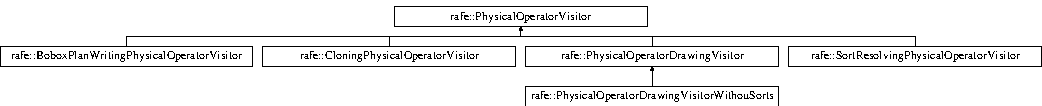
\includegraphics[height=1.409396cm]{classrafe_1_1_physical_operator_visitor}
\end{center}
\end{figure}
\subsection*{Public Member Functions}
\begin{DoxyCompactItemize}
\item 
virtual void \hyperlink{classrafe_1_1_physical_operator_visitor_a516a84d305910f3e1b9d1ae2cb184b24}{visit\+Filter} (\hyperlink{classrafe_1_1_filter}{Filter} $\ast$node)
\item 
virtual void \hyperlink{classrafe_1_1_physical_operator_visitor_a7b581054d167c71fa5443570a6808740}{visit\+Filter\+Keeping\+Order} (\hyperlink{classrafe_1_1_filter_keeping_order}{Filter\+Keeping\+Order} $\ast$node)
\item 
virtual void \hyperlink{classrafe_1_1_physical_operator_visitor_adaee48b1ef175226c860c7b2d70ba15d}{visit\+Sort\+Operator} (\hyperlink{classrafe_1_1_sort_operator}{Sort\+Operator} $\ast$node)
\item 
virtual void \hyperlink{classrafe_1_1_physical_operator_visitor_a9fd16981e6fbb9b545b7edeaabcf97bf}{visit\+Merge\+Equi\+Join} (\hyperlink{classrafe_1_1_merge_equi_join}{Merge\+Equi\+Join} $\ast$node)
\item 
virtual void \hyperlink{classrafe_1_1_physical_operator_visitor_a1d4af9c73ece300d7a90c65481cd8e06}{visit\+Merge\+Non\+Equi\+Join} (\hyperlink{classrafe_1_1_merge_non_equi_join}{Merge\+Non\+Equi\+Join} $\ast$node)
\item 
virtual void \hyperlink{classrafe_1_1_physical_operator_visitor_acc39509ae79aa6848ec928cc4f616d61}{visit\+Cross\+Join} (\hyperlink{classrafe_1_1_cross_join}{Cross\+Join} $\ast$node)
\item 
virtual void \hyperlink{classrafe_1_1_physical_operator_visitor_ae36c9ef817768f134d35fe5b3834855c}{visit\+Hash\+Join} (\hyperlink{classrafe_1_1_hash_join}{Hash\+Join} $\ast$node)
\item 
virtual void \hyperlink{classrafe_1_1_physical_operator_visitor_a9415b5939da4948ac922e63fbece1135}{visit\+Hash\+Anti\+Join} (\hyperlink{classrafe_1_1_hash_anti_join}{Hash\+Anti\+Join} $\ast$node)
\item 
virtual void \hyperlink{classrafe_1_1_physical_operator_visitor_a0f3496aaac992756bbb8f18c1000ed75}{visit\+Merge\+Anti\+Join} (\hyperlink{classrafe_1_1_merge_anti_join}{Merge\+Anti\+Join} $\ast$node)
\item 
virtual void \hyperlink{classrafe_1_1_physical_operator_visitor_a01eb10e07cc1fbe7622bc1eb01fa3b79}{visit\+Union\+Operator} (\hyperlink{classrafe_1_1_union_operator}{Union\+Operator} $\ast$node)
\item 
virtual void \hyperlink{classrafe_1_1_physical_operator_visitor_ab6a2b2b02f2237fd41e6c44f5b2ede9b}{visit\+Hash\+Group} (\hyperlink{classrafe_1_1_hash_group}{Hash\+Group} $\ast$node)
\item 
virtual void \hyperlink{classrafe_1_1_physical_operator_visitor_afb1b6786bf12f12e3b1c2895bf77e874}{visit\+Sorted\+Group} (\hyperlink{classrafe_1_1_sorted_group}{Sorted\+Group} $\ast$node)
\item 
virtual void \hyperlink{classrafe_1_1_physical_operator_visitor_ab69b85d7a2c8f89986d84cbcce6f2f89}{visit\+Columns\+Operations\+Operator} (\hyperlink{classrafe_1_1_columns_operations_operator}{Columns\+Operations\+Operator} $\ast$node)
\item 
virtual void \hyperlink{classrafe_1_1_physical_operator_visitor_a4f8cbef9d1c5a58fceb44deb4a7d998c}{visit\+Scan\+And\+Sort\+By\+Index} (\hyperlink{classrafe_1_1_scan_and_sort_by_index}{Scan\+And\+Sort\+By\+Index} $\ast$node)
\item 
virtual void \hyperlink{classrafe_1_1_physical_operator_visitor_ae3d5b2b56e9465713c5ecd4e5fcea9c9}{visit\+Table\+Scan} (\hyperlink{classrafe_1_1_table_scan}{Table\+Scan} $\ast$node)
\item 
virtual void \hyperlink{classrafe_1_1_physical_operator_visitor_ac33ea100cdb3e642a58a82c4367de3fd}{visit\+Index\+Scan} (\hyperlink{classrafe_1_1_index_scan}{Index\+Scan} $\ast$node)
\end{DoxyCompactItemize}


\subsection{Detailed Description}
Base class for physical operators tree visitors. Every virtual method does nothing only visits node all children. 

\subsection{Member Function Documentation}
\hypertarget{classrafe_1_1_physical_operator_visitor_ab69b85d7a2c8f89986d84cbcce6f2f89}{\index{rafe\+::\+Physical\+Operator\+Visitor@{rafe\+::\+Physical\+Operator\+Visitor}!visit\+Columns\+Operations\+Operator@{visit\+Columns\+Operations\+Operator}}
\index{visit\+Columns\+Operations\+Operator@{visit\+Columns\+Operations\+Operator}!rafe\+::\+Physical\+Operator\+Visitor@{rafe\+::\+Physical\+Operator\+Visitor}}
\subsubsection[{visit\+Columns\+Operations\+Operator}]{\setlength{\rightskip}{0pt plus 5cm}void rafe\+::\+Physical\+Operator\+Visitor\+::visit\+Columns\+Operations\+Operator (
\begin{DoxyParamCaption}
\item[{{\bf Columns\+Operations\+Operator} $\ast$}]{node}
\end{DoxyParamCaption}
)\hspace{0.3cm}{\ttfamily [virtual]}}}\label{classrafe_1_1_physical_operator_visitor_ab69b85d7a2c8f89986d84cbcce6f2f89}
Visits physical operator \hyperlink{classrafe_1_1_columns_operations_operator}{Columns\+Operations\+Operator}. 
\begin{DoxyParams}{Parameters}
{\em node} & visited \hyperlink{classrafe_1_1_columns_operations_operator}{Columns\+Operations\+Operator}. \\
\hline
\end{DoxyParams}


Reimplemented in \hyperlink{classrafe_1_1_bobox_plan_writing_physical_operator_visitor_a38591cef68b9a97fc8e854827d33103b}{rafe\+::\+Bobox\+Plan\+Writing\+Physical\+Operator\+Visitor}, \hyperlink{classrafe_1_1_sort_resolving_physical_operator_visitor_a6ad430ddefd7a5f9f5a393d76dabc6db}{rafe\+::\+Sort\+Resolving\+Physical\+Operator\+Visitor}, \hyperlink{classrafe_1_1_cloning_physical_operator_visitor_aac8214c9491fac739850b004bad92815}{rafe\+::\+Cloning\+Physical\+Operator\+Visitor}, and \hyperlink{classrafe_1_1_physical_operator_drawing_visitor_a9c12b247be5746314eb74747bc5d50af}{rafe\+::\+Physical\+Operator\+Drawing\+Visitor}.

\hypertarget{classrafe_1_1_physical_operator_visitor_acc39509ae79aa6848ec928cc4f616d61}{\index{rafe\+::\+Physical\+Operator\+Visitor@{rafe\+::\+Physical\+Operator\+Visitor}!visit\+Cross\+Join@{visit\+Cross\+Join}}
\index{visit\+Cross\+Join@{visit\+Cross\+Join}!rafe\+::\+Physical\+Operator\+Visitor@{rafe\+::\+Physical\+Operator\+Visitor}}
\subsubsection[{visit\+Cross\+Join}]{\setlength{\rightskip}{0pt plus 5cm}void rafe\+::\+Physical\+Operator\+Visitor\+::visit\+Cross\+Join (
\begin{DoxyParamCaption}
\item[{{\bf Cross\+Join} $\ast$}]{node}
\end{DoxyParamCaption}
)\hspace{0.3cm}{\ttfamily [virtual]}}}\label{classrafe_1_1_physical_operator_visitor_acc39509ae79aa6848ec928cc4f616d61}
Visits physical operator \hyperlink{classrafe_1_1_cross_join}{Cross\+Join}. 
\begin{DoxyParams}{Parameters}
{\em node} & visited \hyperlink{classrafe_1_1_cross_join}{Cross\+Join}. \\
\hline
\end{DoxyParams}


Reimplemented in \hyperlink{classrafe_1_1_bobox_plan_writing_physical_operator_visitor_af8ff4c17855ea7872ed2871aa317591d}{rafe\+::\+Bobox\+Plan\+Writing\+Physical\+Operator\+Visitor}, \hyperlink{classrafe_1_1_sort_resolving_physical_operator_visitor_a5c99705870fc4476ed1130d9d947270d}{rafe\+::\+Sort\+Resolving\+Physical\+Operator\+Visitor}, \hyperlink{classrafe_1_1_cloning_physical_operator_visitor_ab0ce6e1f5d26047f898603aeb39278f6}{rafe\+::\+Cloning\+Physical\+Operator\+Visitor}, and \hyperlink{classrafe_1_1_physical_operator_drawing_visitor_ae10d5b2b254263a0a206ba8056799746}{rafe\+::\+Physical\+Operator\+Drawing\+Visitor}.

\hypertarget{classrafe_1_1_physical_operator_visitor_a516a84d305910f3e1b9d1ae2cb184b24}{\index{rafe\+::\+Physical\+Operator\+Visitor@{rafe\+::\+Physical\+Operator\+Visitor}!visit\+Filter@{visit\+Filter}}
\index{visit\+Filter@{visit\+Filter}!rafe\+::\+Physical\+Operator\+Visitor@{rafe\+::\+Physical\+Operator\+Visitor}}
\subsubsection[{visit\+Filter}]{\setlength{\rightskip}{0pt plus 5cm}void rafe\+::\+Physical\+Operator\+Visitor\+::visit\+Filter (
\begin{DoxyParamCaption}
\item[{{\bf Filter} $\ast$}]{node}
\end{DoxyParamCaption}
)\hspace{0.3cm}{\ttfamily [virtual]}}}\label{classrafe_1_1_physical_operator_visitor_a516a84d305910f3e1b9d1ae2cb184b24}
Visits physical operator \hyperlink{classrafe_1_1_filter}{Filter}. 
\begin{DoxyParams}{Parameters}
{\em node} & visited \hyperlink{classrafe_1_1_filter}{Filter}. \\
\hline
\end{DoxyParams}


Reimplemented in \hyperlink{classrafe_1_1_bobox_plan_writing_physical_operator_visitor_a729ee192bceef48ed5221447427be2a4}{rafe\+::\+Bobox\+Plan\+Writing\+Physical\+Operator\+Visitor}, \hyperlink{classrafe_1_1_sort_resolving_physical_operator_visitor_a925504a20a6cbe1d5fd4e1ffb2ed2c56}{rafe\+::\+Sort\+Resolving\+Physical\+Operator\+Visitor}, \hyperlink{classrafe_1_1_cloning_physical_operator_visitor_a81fb87714996a1e029da452d2b57796c}{rafe\+::\+Cloning\+Physical\+Operator\+Visitor}, and \hyperlink{classrafe_1_1_physical_operator_drawing_visitor_a8c34db1b84ad6fb8c8de4b5a27542062}{rafe\+::\+Physical\+Operator\+Drawing\+Visitor}.

\hypertarget{classrafe_1_1_physical_operator_visitor_a7b581054d167c71fa5443570a6808740}{\index{rafe\+::\+Physical\+Operator\+Visitor@{rafe\+::\+Physical\+Operator\+Visitor}!visit\+Filter\+Keeping\+Order@{visit\+Filter\+Keeping\+Order}}
\index{visit\+Filter\+Keeping\+Order@{visit\+Filter\+Keeping\+Order}!rafe\+::\+Physical\+Operator\+Visitor@{rafe\+::\+Physical\+Operator\+Visitor}}
\subsubsection[{visit\+Filter\+Keeping\+Order}]{\setlength{\rightskip}{0pt plus 5cm}void rafe\+::\+Physical\+Operator\+Visitor\+::visit\+Filter\+Keeping\+Order (
\begin{DoxyParamCaption}
\item[{{\bf Filter\+Keeping\+Order} $\ast$}]{node}
\end{DoxyParamCaption}
)\hspace{0.3cm}{\ttfamily [virtual]}}}\label{classrafe_1_1_physical_operator_visitor_a7b581054d167c71fa5443570a6808740}
Visits physical operator \hyperlink{classrafe_1_1_filter_keeping_order}{Filter\+Keeping\+Order}. 
\begin{DoxyParams}{Parameters}
{\em node} & visited \hyperlink{classrafe_1_1_filter_keeping_order}{Filter\+Keeping\+Order}. \\
\hline
\end{DoxyParams}


Reimplemented in \hyperlink{classrafe_1_1_bobox_plan_writing_physical_operator_visitor_a34f3d494a32fdc1e694ea4568f09db28}{rafe\+::\+Bobox\+Plan\+Writing\+Physical\+Operator\+Visitor}, \hyperlink{classrafe_1_1_sort_resolving_physical_operator_visitor_a1d2b21ae0c554fa5dc3953c144de2bbd}{rafe\+::\+Sort\+Resolving\+Physical\+Operator\+Visitor}, \hyperlink{classrafe_1_1_cloning_physical_operator_visitor_a885c7ea7353edd39752618c3ae4000ec}{rafe\+::\+Cloning\+Physical\+Operator\+Visitor}, and \hyperlink{classrafe_1_1_physical_operator_drawing_visitor_ad354fa6a9a6b139e893e4827ff2ecf3d}{rafe\+::\+Physical\+Operator\+Drawing\+Visitor}.

\hypertarget{classrafe_1_1_physical_operator_visitor_a9415b5939da4948ac922e63fbece1135}{\index{rafe\+::\+Physical\+Operator\+Visitor@{rafe\+::\+Physical\+Operator\+Visitor}!visit\+Hash\+Anti\+Join@{visit\+Hash\+Anti\+Join}}
\index{visit\+Hash\+Anti\+Join@{visit\+Hash\+Anti\+Join}!rafe\+::\+Physical\+Operator\+Visitor@{rafe\+::\+Physical\+Operator\+Visitor}}
\subsubsection[{visit\+Hash\+Anti\+Join}]{\setlength{\rightskip}{0pt plus 5cm}void rafe\+::\+Physical\+Operator\+Visitor\+::visit\+Hash\+Anti\+Join (
\begin{DoxyParamCaption}
\item[{{\bf Hash\+Anti\+Join} $\ast$}]{node}
\end{DoxyParamCaption}
)\hspace{0.3cm}{\ttfamily [virtual]}}}\label{classrafe_1_1_physical_operator_visitor_a9415b5939da4948ac922e63fbece1135}
Visits physical operator \hyperlink{classrafe_1_1_hash_anti_join}{Hash\+Anti\+Join}. 
\begin{DoxyParams}{Parameters}
{\em node} & visited \hyperlink{classrafe_1_1_hash_anti_join}{Hash\+Anti\+Join}. \\
\hline
\end{DoxyParams}


Reimplemented in \hyperlink{classrafe_1_1_bobox_plan_writing_physical_operator_visitor_a4c75cb58ec95bc07e9923a3b7c0c2175}{rafe\+::\+Bobox\+Plan\+Writing\+Physical\+Operator\+Visitor}, \hyperlink{classrafe_1_1_sort_resolving_physical_operator_visitor_aa40215b7f2fd2fba9b6d82198e256972}{rafe\+::\+Sort\+Resolving\+Physical\+Operator\+Visitor}, \hyperlink{classrafe_1_1_cloning_physical_operator_visitor_a19461012b1f6c83d7b27361b02bf6a7d}{rafe\+::\+Cloning\+Physical\+Operator\+Visitor}, and \hyperlink{classrafe_1_1_physical_operator_drawing_visitor_aaff4651c152fd3d86805014459f5f565}{rafe\+::\+Physical\+Operator\+Drawing\+Visitor}.

\hypertarget{classrafe_1_1_physical_operator_visitor_ab6a2b2b02f2237fd41e6c44f5b2ede9b}{\index{rafe\+::\+Physical\+Operator\+Visitor@{rafe\+::\+Physical\+Operator\+Visitor}!visit\+Hash\+Group@{visit\+Hash\+Group}}
\index{visit\+Hash\+Group@{visit\+Hash\+Group}!rafe\+::\+Physical\+Operator\+Visitor@{rafe\+::\+Physical\+Operator\+Visitor}}
\subsubsection[{visit\+Hash\+Group}]{\setlength{\rightskip}{0pt plus 5cm}void rafe\+::\+Physical\+Operator\+Visitor\+::visit\+Hash\+Group (
\begin{DoxyParamCaption}
\item[{{\bf Hash\+Group} $\ast$}]{node}
\end{DoxyParamCaption}
)\hspace{0.3cm}{\ttfamily [virtual]}}}\label{classrafe_1_1_physical_operator_visitor_ab6a2b2b02f2237fd41e6c44f5b2ede9b}
Visits physical operator \hyperlink{classrafe_1_1_hash_group}{Hash\+Group}. 
\begin{DoxyParams}{Parameters}
{\em node} & visited \hyperlink{classrafe_1_1_hash_group}{Hash\+Group}. \\
\hline
\end{DoxyParams}


Reimplemented in \hyperlink{classrafe_1_1_bobox_plan_writing_physical_operator_visitor_a8f9890744b4a3a64e1d574d4d12bc1ca}{rafe\+::\+Bobox\+Plan\+Writing\+Physical\+Operator\+Visitor}, \hyperlink{classrafe_1_1_sort_resolving_physical_operator_visitor_ab2ed3da0ba8c7ba6c6f57af128b93979}{rafe\+::\+Sort\+Resolving\+Physical\+Operator\+Visitor}, \hyperlink{classrafe_1_1_cloning_physical_operator_visitor_a489a807271ce26529d48cefea1aa31a2}{rafe\+::\+Cloning\+Physical\+Operator\+Visitor}, and \hyperlink{classrafe_1_1_physical_operator_drawing_visitor_a81ede5f72bee22e9885236c8056a4556}{rafe\+::\+Physical\+Operator\+Drawing\+Visitor}.

\hypertarget{classrafe_1_1_physical_operator_visitor_ae36c9ef817768f134d35fe5b3834855c}{\index{rafe\+::\+Physical\+Operator\+Visitor@{rafe\+::\+Physical\+Operator\+Visitor}!visit\+Hash\+Join@{visit\+Hash\+Join}}
\index{visit\+Hash\+Join@{visit\+Hash\+Join}!rafe\+::\+Physical\+Operator\+Visitor@{rafe\+::\+Physical\+Operator\+Visitor}}
\subsubsection[{visit\+Hash\+Join}]{\setlength{\rightskip}{0pt plus 5cm}void rafe\+::\+Physical\+Operator\+Visitor\+::visit\+Hash\+Join (
\begin{DoxyParamCaption}
\item[{{\bf Hash\+Join} $\ast$}]{node}
\end{DoxyParamCaption}
)\hspace{0.3cm}{\ttfamily [virtual]}}}\label{classrafe_1_1_physical_operator_visitor_ae36c9ef817768f134d35fe5b3834855c}
Visits physical operator \hyperlink{classrafe_1_1_hash_join}{Hash\+Join}. 
\begin{DoxyParams}{Parameters}
{\em node} & visited \hyperlink{classrafe_1_1_hash_join}{Hash\+Join}. \\
\hline
\end{DoxyParams}


Reimplemented in \hyperlink{classrafe_1_1_bobox_plan_writing_physical_operator_visitor_ad0924de22102447e0e6c38a90432f3c6}{rafe\+::\+Bobox\+Plan\+Writing\+Physical\+Operator\+Visitor}, \hyperlink{classrafe_1_1_sort_resolving_physical_operator_visitor_a8a19661db996874c0f3ab97e0dbf57c0}{rafe\+::\+Sort\+Resolving\+Physical\+Operator\+Visitor}, \hyperlink{classrafe_1_1_cloning_physical_operator_visitor_aad57f1f45fa9f3c6633db5421f17774e}{rafe\+::\+Cloning\+Physical\+Operator\+Visitor}, and \hyperlink{classrafe_1_1_physical_operator_drawing_visitor_ac4be6a3ffbb85fd1d7a7f5ec109277ca}{rafe\+::\+Physical\+Operator\+Drawing\+Visitor}.

\hypertarget{classrafe_1_1_physical_operator_visitor_ac33ea100cdb3e642a58a82c4367de3fd}{\index{rafe\+::\+Physical\+Operator\+Visitor@{rafe\+::\+Physical\+Operator\+Visitor}!visit\+Index\+Scan@{visit\+Index\+Scan}}
\index{visit\+Index\+Scan@{visit\+Index\+Scan}!rafe\+::\+Physical\+Operator\+Visitor@{rafe\+::\+Physical\+Operator\+Visitor}}
\subsubsection[{visit\+Index\+Scan}]{\setlength{\rightskip}{0pt plus 5cm}void rafe\+::\+Physical\+Operator\+Visitor\+::visit\+Index\+Scan (
\begin{DoxyParamCaption}
\item[{{\bf Index\+Scan} $\ast$}]{node}
\end{DoxyParamCaption}
)\hspace{0.3cm}{\ttfamily [virtual]}}}\label{classrafe_1_1_physical_operator_visitor_ac33ea100cdb3e642a58a82c4367de3fd}
Visits physical operator \hyperlink{classrafe_1_1_index_scan}{Index\+Scan}. 
\begin{DoxyParams}{Parameters}
{\em node} & visited \hyperlink{classrafe_1_1_index_scan}{Index\+Scan}. \\
\hline
\end{DoxyParams}


Reimplemented in \hyperlink{classrafe_1_1_bobox_plan_writing_physical_operator_visitor_a600bfeaec99ab68049069543bad70908}{rafe\+::\+Bobox\+Plan\+Writing\+Physical\+Operator\+Visitor}, \hyperlink{classrafe_1_1_sort_resolving_physical_operator_visitor_a751dc6fc9c39542497d85b866549c895}{rafe\+::\+Sort\+Resolving\+Physical\+Operator\+Visitor}, \hyperlink{classrafe_1_1_cloning_physical_operator_visitor_a43fa4aac2e3adfd4b1dc2280a1cfe165}{rafe\+::\+Cloning\+Physical\+Operator\+Visitor}, and \hyperlink{classrafe_1_1_physical_operator_drawing_visitor_a6a74e5a271b3ab7ed954a2821f7dbcc9}{rafe\+::\+Physical\+Operator\+Drawing\+Visitor}.

\hypertarget{classrafe_1_1_physical_operator_visitor_a0f3496aaac992756bbb8f18c1000ed75}{\index{rafe\+::\+Physical\+Operator\+Visitor@{rafe\+::\+Physical\+Operator\+Visitor}!visit\+Merge\+Anti\+Join@{visit\+Merge\+Anti\+Join}}
\index{visit\+Merge\+Anti\+Join@{visit\+Merge\+Anti\+Join}!rafe\+::\+Physical\+Operator\+Visitor@{rafe\+::\+Physical\+Operator\+Visitor}}
\subsubsection[{visit\+Merge\+Anti\+Join}]{\setlength{\rightskip}{0pt plus 5cm}void rafe\+::\+Physical\+Operator\+Visitor\+::visit\+Merge\+Anti\+Join (
\begin{DoxyParamCaption}
\item[{{\bf Merge\+Anti\+Join} $\ast$}]{node}
\end{DoxyParamCaption}
)\hspace{0.3cm}{\ttfamily [virtual]}}}\label{classrafe_1_1_physical_operator_visitor_a0f3496aaac992756bbb8f18c1000ed75}
Visits physical operator \hyperlink{classrafe_1_1_merge_anti_join}{Merge\+Anti\+Join}. 
\begin{DoxyParams}{Parameters}
{\em node} & visited \hyperlink{classrafe_1_1_merge_anti_join}{Merge\+Anti\+Join}. \\
\hline
\end{DoxyParams}


Reimplemented in \hyperlink{classrafe_1_1_bobox_plan_writing_physical_operator_visitor_a44f741c5e3ad55bdb934641371057000}{rafe\+::\+Bobox\+Plan\+Writing\+Physical\+Operator\+Visitor}, \hyperlink{classrafe_1_1_sort_resolving_physical_operator_visitor_aea8f22d3c2f4e3f13012c577c5f74e3a}{rafe\+::\+Sort\+Resolving\+Physical\+Operator\+Visitor}, \hyperlink{classrafe_1_1_cloning_physical_operator_visitor_a7e306d085f9a1c0a0cbe7befc79b7e97}{rafe\+::\+Cloning\+Physical\+Operator\+Visitor}, and \hyperlink{classrafe_1_1_physical_operator_drawing_visitor_a048897346f3a1344cab951f3d3ef7394}{rafe\+::\+Physical\+Operator\+Drawing\+Visitor}.

\hypertarget{classrafe_1_1_physical_operator_visitor_a9fd16981e6fbb9b545b7edeaabcf97bf}{\index{rafe\+::\+Physical\+Operator\+Visitor@{rafe\+::\+Physical\+Operator\+Visitor}!visit\+Merge\+Equi\+Join@{visit\+Merge\+Equi\+Join}}
\index{visit\+Merge\+Equi\+Join@{visit\+Merge\+Equi\+Join}!rafe\+::\+Physical\+Operator\+Visitor@{rafe\+::\+Physical\+Operator\+Visitor}}
\subsubsection[{visit\+Merge\+Equi\+Join}]{\setlength{\rightskip}{0pt plus 5cm}void rafe\+::\+Physical\+Operator\+Visitor\+::visit\+Merge\+Equi\+Join (
\begin{DoxyParamCaption}
\item[{{\bf Merge\+Equi\+Join} $\ast$}]{node}
\end{DoxyParamCaption}
)\hspace{0.3cm}{\ttfamily [virtual]}}}\label{classrafe_1_1_physical_operator_visitor_a9fd16981e6fbb9b545b7edeaabcf97bf}
Visits physical operator \hyperlink{classrafe_1_1_merge_equi_join}{Merge\+Equi\+Join}. 
\begin{DoxyParams}{Parameters}
{\em node} & visited \hyperlink{classrafe_1_1_merge_equi_join}{Merge\+Equi\+Join}. \\
\hline
\end{DoxyParams}


Reimplemented in \hyperlink{classrafe_1_1_bobox_plan_writing_physical_operator_visitor_a424e82f02063f08ec2849a4728f49b83}{rafe\+::\+Bobox\+Plan\+Writing\+Physical\+Operator\+Visitor}, \hyperlink{classrafe_1_1_sort_resolving_physical_operator_visitor_af3c9ea7f184b65db3c23122732c40a1c}{rafe\+::\+Sort\+Resolving\+Physical\+Operator\+Visitor}, \hyperlink{classrafe_1_1_cloning_physical_operator_visitor_af940eb33c8b37ec531254bbb14d2d2a9}{rafe\+::\+Cloning\+Physical\+Operator\+Visitor}, and \hyperlink{classrafe_1_1_physical_operator_drawing_visitor_aaa61a390184345f77b3d7d731f5eb042}{rafe\+::\+Physical\+Operator\+Drawing\+Visitor}.

\hypertarget{classrafe_1_1_physical_operator_visitor_a1d4af9c73ece300d7a90c65481cd8e06}{\index{rafe\+::\+Physical\+Operator\+Visitor@{rafe\+::\+Physical\+Operator\+Visitor}!visit\+Merge\+Non\+Equi\+Join@{visit\+Merge\+Non\+Equi\+Join}}
\index{visit\+Merge\+Non\+Equi\+Join@{visit\+Merge\+Non\+Equi\+Join}!rafe\+::\+Physical\+Operator\+Visitor@{rafe\+::\+Physical\+Operator\+Visitor}}
\subsubsection[{visit\+Merge\+Non\+Equi\+Join}]{\setlength{\rightskip}{0pt plus 5cm}void rafe\+::\+Physical\+Operator\+Visitor\+::visit\+Merge\+Non\+Equi\+Join (
\begin{DoxyParamCaption}
\item[{{\bf Merge\+Non\+Equi\+Join} $\ast$}]{node}
\end{DoxyParamCaption}
)\hspace{0.3cm}{\ttfamily [virtual]}}}\label{classrafe_1_1_physical_operator_visitor_a1d4af9c73ece300d7a90c65481cd8e06}
Visits physical operator \hyperlink{classrafe_1_1_merge_non_equi_join}{Merge\+Non\+Equi\+Join}. 
\begin{DoxyParams}{Parameters}
{\em node} & visited \hyperlink{classrafe_1_1_merge_non_equi_join}{Merge\+Non\+Equi\+Join}. \\
\hline
\end{DoxyParams}


Reimplemented in \hyperlink{classrafe_1_1_bobox_plan_writing_physical_operator_visitor_af9342d338c7b1f83e4c6bb2250915adc}{rafe\+::\+Bobox\+Plan\+Writing\+Physical\+Operator\+Visitor}, \hyperlink{classrafe_1_1_sort_resolving_physical_operator_visitor_aa9fa7d5ee61fadf7e4a9c36be172b0f2}{rafe\+::\+Sort\+Resolving\+Physical\+Operator\+Visitor}, \hyperlink{classrafe_1_1_cloning_physical_operator_visitor_a9d91a81c0a4e620fb96532388f69bfa1}{rafe\+::\+Cloning\+Physical\+Operator\+Visitor}, and \hyperlink{classrafe_1_1_physical_operator_drawing_visitor_ade0f29c6899eddf9fca59013eb079ac3}{rafe\+::\+Physical\+Operator\+Drawing\+Visitor}.

\hypertarget{classrafe_1_1_physical_operator_visitor_a4f8cbef9d1c5a58fceb44deb4a7d998c}{\index{rafe\+::\+Physical\+Operator\+Visitor@{rafe\+::\+Physical\+Operator\+Visitor}!visit\+Scan\+And\+Sort\+By\+Index@{visit\+Scan\+And\+Sort\+By\+Index}}
\index{visit\+Scan\+And\+Sort\+By\+Index@{visit\+Scan\+And\+Sort\+By\+Index}!rafe\+::\+Physical\+Operator\+Visitor@{rafe\+::\+Physical\+Operator\+Visitor}}
\subsubsection[{visit\+Scan\+And\+Sort\+By\+Index}]{\setlength{\rightskip}{0pt plus 5cm}void rafe\+::\+Physical\+Operator\+Visitor\+::visit\+Scan\+And\+Sort\+By\+Index (
\begin{DoxyParamCaption}
\item[{{\bf Scan\+And\+Sort\+By\+Index} $\ast$}]{node}
\end{DoxyParamCaption}
)\hspace{0.3cm}{\ttfamily [virtual]}}}\label{classrafe_1_1_physical_operator_visitor_a4f8cbef9d1c5a58fceb44deb4a7d998c}
Visits physical operator \hyperlink{classrafe_1_1_scan_and_sort_by_index}{Scan\+And\+Sort\+By\+Index}. 
\begin{DoxyParams}{Parameters}
{\em node} & visited \hyperlink{classrafe_1_1_scan_and_sort_by_index}{Scan\+And\+Sort\+By\+Index}. \\
\hline
\end{DoxyParams}


Reimplemented in \hyperlink{classrafe_1_1_bobox_plan_writing_physical_operator_visitor_a747d8a89471bcf19b29d4eb8f9be5196}{rafe\+::\+Bobox\+Plan\+Writing\+Physical\+Operator\+Visitor}, \hyperlink{classrafe_1_1_sort_resolving_physical_operator_visitor_a14698876ca3eae58a6f40f1e0d0dca13}{rafe\+::\+Sort\+Resolving\+Physical\+Operator\+Visitor}, \hyperlink{classrafe_1_1_cloning_physical_operator_visitor_a61e925129b55230d187280a9a6d76d37}{rafe\+::\+Cloning\+Physical\+Operator\+Visitor}, and \hyperlink{classrafe_1_1_physical_operator_drawing_visitor_abd677a519edaf4df41a7a32c7e0fd0cf}{rafe\+::\+Physical\+Operator\+Drawing\+Visitor}.

\hypertarget{classrafe_1_1_physical_operator_visitor_afb1b6786bf12f12e3b1c2895bf77e874}{\index{rafe\+::\+Physical\+Operator\+Visitor@{rafe\+::\+Physical\+Operator\+Visitor}!visit\+Sorted\+Group@{visit\+Sorted\+Group}}
\index{visit\+Sorted\+Group@{visit\+Sorted\+Group}!rafe\+::\+Physical\+Operator\+Visitor@{rafe\+::\+Physical\+Operator\+Visitor}}
\subsubsection[{visit\+Sorted\+Group}]{\setlength{\rightskip}{0pt plus 5cm}void rafe\+::\+Physical\+Operator\+Visitor\+::visit\+Sorted\+Group (
\begin{DoxyParamCaption}
\item[{{\bf Sorted\+Group} $\ast$}]{node}
\end{DoxyParamCaption}
)\hspace{0.3cm}{\ttfamily [virtual]}}}\label{classrafe_1_1_physical_operator_visitor_afb1b6786bf12f12e3b1c2895bf77e874}
Visits physical operator \hyperlink{classrafe_1_1_sorted_group}{Sorted\+Group}. 
\begin{DoxyParams}{Parameters}
{\em node} & visited \hyperlink{classrafe_1_1_sorted_group}{Sorted\+Group}. \\
\hline
\end{DoxyParams}


Reimplemented in \hyperlink{classrafe_1_1_bobox_plan_writing_physical_operator_visitor_ab0f53218eefa3103840afe5bf7fcf9ab}{rafe\+::\+Bobox\+Plan\+Writing\+Physical\+Operator\+Visitor}, \hyperlink{classrafe_1_1_sort_resolving_physical_operator_visitor_a236a97d59e960a5612758f97342758c8}{rafe\+::\+Sort\+Resolving\+Physical\+Operator\+Visitor}, \hyperlink{classrafe_1_1_cloning_physical_operator_visitor_a5eeb41c81760f9598b11e18ba26949f6}{rafe\+::\+Cloning\+Physical\+Operator\+Visitor}, and \hyperlink{classrafe_1_1_physical_operator_drawing_visitor_a5df8d5fca216ef12f6d9b836a310797f}{rafe\+::\+Physical\+Operator\+Drawing\+Visitor}.

\hypertarget{classrafe_1_1_physical_operator_visitor_adaee48b1ef175226c860c7b2d70ba15d}{\index{rafe\+::\+Physical\+Operator\+Visitor@{rafe\+::\+Physical\+Operator\+Visitor}!visit\+Sort\+Operator@{visit\+Sort\+Operator}}
\index{visit\+Sort\+Operator@{visit\+Sort\+Operator}!rafe\+::\+Physical\+Operator\+Visitor@{rafe\+::\+Physical\+Operator\+Visitor}}
\subsubsection[{visit\+Sort\+Operator}]{\setlength{\rightskip}{0pt plus 5cm}void rafe\+::\+Physical\+Operator\+Visitor\+::visit\+Sort\+Operator (
\begin{DoxyParamCaption}
\item[{{\bf Sort\+Operator} $\ast$}]{node}
\end{DoxyParamCaption}
)\hspace{0.3cm}{\ttfamily [virtual]}}}\label{classrafe_1_1_physical_operator_visitor_adaee48b1ef175226c860c7b2d70ba15d}
Visits physical operator \hyperlink{classrafe_1_1_sort_operator}{Sort\+Operator}. 
\begin{DoxyParams}{Parameters}
{\em node} & visited \hyperlink{classrafe_1_1_sort_operator}{Sort\+Operator}. \\
\hline
\end{DoxyParams}


Reimplemented in \hyperlink{classrafe_1_1_bobox_plan_writing_physical_operator_visitor_a63be13a7222bfdb4a317334b0b2f892d}{rafe\+::\+Bobox\+Plan\+Writing\+Physical\+Operator\+Visitor}, \hyperlink{classrafe_1_1_sort_resolving_physical_operator_visitor_aa7eb1c55a79f893f09c6e32ebaae3175}{rafe\+::\+Sort\+Resolving\+Physical\+Operator\+Visitor}, \hyperlink{classrafe_1_1_cloning_physical_operator_visitor_afd4177f24dc58c451d2ca2ce5ed74683}{rafe\+::\+Cloning\+Physical\+Operator\+Visitor}, and \hyperlink{classrafe_1_1_physical_operator_drawing_visitor_a1d9f4efce36cd996b4d969e12f926560}{rafe\+::\+Physical\+Operator\+Drawing\+Visitor}.

\hypertarget{classrafe_1_1_physical_operator_visitor_ae3d5b2b56e9465713c5ecd4e5fcea9c9}{\index{rafe\+::\+Physical\+Operator\+Visitor@{rafe\+::\+Physical\+Operator\+Visitor}!visit\+Table\+Scan@{visit\+Table\+Scan}}
\index{visit\+Table\+Scan@{visit\+Table\+Scan}!rafe\+::\+Physical\+Operator\+Visitor@{rafe\+::\+Physical\+Operator\+Visitor}}
\subsubsection[{visit\+Table\+Scan}]{\setlength{\rightskip}{0pt plus 5cm}void rafe\+::\+Physical\+Operator\+Visitor\+::visit\+Table\+Scan (
\begin{DoxyParamCaption}
\item[{{\bf Table\+Scan} $\ast$}]{node}
\end{DoxyParamCaption}
)\hspace{0.3cm}{\ttfamily [virtual]}}}\label{classrafe_1_1_physical_operator_visitor_ae3d5b2b56e9465713c5ecd4e5fcea9c9}
Visits physical operator \hyperlink{classrafe_1_1_table_scan}{Table\+Scan}. 
\begin{DoxyParams}{Parameters}
{\em node} & visited \hyperlink{classrafe_1_1_table_scan}{Table\+Scan}. \\
\hline
\end{DoxyParams}


Reimplemented in \hyperlink{classrafe_1_1_bobox_plan_writing_physical_operator_visitor_ab7918b1aa4d801ec86d42b3cbb6d0fe1}{rafe\+::\+Bobox\+Plan\+Writing\+Physical\+Operator\+Visitor}, \hyperlink{classrafe_1_1_sort_resolving_physical_operator_visitor_a5d481f69e9982db492fc899693cf1714}{rafe\+::\+Sort\+Resolving\+Physical\+Operator\+Visitor}, \hyperlink{classrafe_1_1_cloning_physical_operator_visitor_a5515f4184243db8a585276d1cb58a8c2}{rafe\+::\+Cloning\+Physical\+Operator\+Visitor}, and \hyperlink{classrafe_1_1_physical_operator_drawing_visitor_a0c61159c63401e8a96645a277459650e}{rafe\+::\+Physical\+Operator\+Drawing\+Visitor}.

\hypertarget{classrafe_1_1_physical_operator_visitor_a01eb10e07cc1fbe7622bc1eb01fa3b79}{\index{rafe\+::\+Physical\+Operator\+Visitor@{rafe\+::\+Physical\+Operator\+Visitor}!visit\+Union\+Operator@{visit\+Union\+Operator}}
\index{visit\+Union\+Operator@{visit\+Union\+Operator}!rafe\+::\+Physical\+Operator\+Visitor@{rafe\+::\+Physical\+Operator\+Visitor}}
\subsubsection[{visit\+Union\+Operator}]{\setlength{\rightskip}{0pt plus 5cm}void rafe\+::\+Physical\+Operator\+Visitor\+::visit\+Union\+Operator (
\begin{DoxyParamCaption}
\item[{{\bf Union\+Operator} $\ast$}]{node}
\end{DoxyParamCaption}
)\hspace{0.3cm}{\ttfamily [virtual]}}}\label{classrafe_1_1_physical_operator_visitor_a01eb10e07cc1fbe7622bc1eb01fa3b79}
Visits physical operator \hyperlink{classrafe_1_1_union_operator}{Union\+Operator}. 
\begin{DoxyParams}{Parameters}
{\em node} & visited \hyperlink{classrafe_1_1_union_operator}{Union\+Operator}. \\
\hline
\end{DoxyParams}


Reimplemented in \hyperlink{classrafe_1_1_bobox_plan_writing_physical_operator_visitor_a20fc58d77f1fba7b536bd8c0920641c5}{rafe\+::\+Bobox\+Plan\+Writing\+Physical\+Operator\+Visitor}, \hyperlink{classrafe_1_1_sort_resolving_physical_operator_visitor_ac04fc55c4e6ba70e29f2bf43fb2912dc}{rafe\+::\+Sort\+Resolving\+Physical\+Operator\+Visitor}, \hyperlink{classrafe_1_1_cloning_physical_operator_visitor_ad8ec858f208334b140f5cb95a01c4063}{rafe\+::\+Cloning\+Physical\+Operator\+Visitor}, and \hyperlink{classrafe_1_1_physical_operator_drawing_visitor_a9d9921709b02d719159ea0990f041ddd}{rafe\+::\+Physical\+Operator\+Drawing\+Visitor}.



The documentation for this class was generated from the following files\+:\begin{DoxyCompactItemize}
\item 
C\+:/\+Users/\+Marcel/\+Documents/\+Visual Studio 2012/\+Projects/\+Relational\+Query\+Evaluator/\+Relational\+Query\+Evaluator/Physical\+Operator\+Visitor.\+h\item 
C\+:/\+Users/\+Marcel/\+Documents/\+Visual Studio 2012/\+Projects/\+Relational\+Query\+Evaluator/\+Relational\+Query\+Evaluator/Physical\+Operator\+Visitor.\+cpp\end{DoxyCompactItemize}

\hypertarget{classrafe_1_1_physical_plan}{\section{rafe\+:\+:Physical\+Plan Class Reference}
\label{classrafe_1_1_physical_plan}\index{rafe\+::\+Physical\+Plan@{rafe\+::\+Physical\+Plan}}
}


{\ttfamily \#include $<$Physical\+Operator.\+h$>$}

\subsection*{Public Member Functions}
\begin{DoxyCompactItemize}
\item 
\hyperlink{classrafe_1_1_physical_plan_a0084a98932e4918feb1e46c83973c279}{Physical\+Plan} ()
\item 
\hyperlink{classrafe_1_1_physical_plan_a7b1653d5f6e19a477470ccc52139a9ac}{Physical\+Plan} (\hyperlink{classrafe_1_1_nullary_physical_operator}{Nullary\+Physical\+Operator} $\ast$op, double number\+Of\+Rows, double time, std\+::vector$<$ \hyperlink{classrafe_1_1_column_info}{Column\+Info} $>$ \&cols)
\item 
\hyperlink{classrafe_1_1_physical_plan_a869d7b418f71ba491042bfee7283beee}{Physical\+Plan} (\hyperlink{classrafe_1_1_nullary_physical_operator}{Nullary\+Physical\+Operator} $\ast$op, double number\+Of\+Rows, double time, const std\+::map$<$ int, \hyperlink{classrafe_1_1_column_info}{Column\+Info} $>$ \&new\+Columns)
\item 
\hyperlink{classrafe_1_1_physical_plan_aed48c874435c06aa80245eb103cd5242}{Physical\+Plan} (\hyperlink{classrafe_1_1_unary_physical_operator}{Unary\+Physical\+Operator} $\ast$op, double new\+Size, double time, const std\+::map$<$ int, \hyperlink{classrafe_1_1_column_info}{Column\+Info} $>$ \&new\+Columns, const std\+::shared\+\_\+ptr$<$ \hyperlink{classrafe_1_1_physical_plan}{Physical\+Plan} $>$ \&old\+Plan)
\item 
\hyperlink{classrafe_1_1_physical_plan_a2d944eb6010f2c04bc3e6f8cfb0bdd16}{Physical\+Plan} (\hyperlink{classrafe_1_1_binary_physical_operator}{Binary\+Physical\+Operator} $\ast$op, double new\+Size, double time, const std\+::map$<$ int, \hyperlink{classrafe_1_1_column_info}{Column\+Info} $>$ \&new\+Columns, const std\+::shared\+\_\+ptr$<$ \hyperlink{classrafe_1_1_physical_plan}{Physical\+Plan} $>$ \&old\+Plan1, const std\+::shared\+\_\+ptr$<$ \hyperlink{classrafe_1_1_physical_plan}{Physical\+Plan} $>$ \&old\+Plan2)
\end{DoxyCompactItemize}
\subsection*{Static Public Member Functions}
\begin{DoxyCompactItemize}
\item 
static bool \hyperlink{classrafe_1_1_physical_plan_acde8212fd29787b0fef4db7a080f70d3}{Comparator} (std\+::shared\+\_\+ptr$<$ \hyperlink{classrafe_1_1_physical_plan}{Physical\+Plan} $>$ \&i, std\+::shared\+\_\+ptr$<$ \hyperlink{classrafe_1_1_physical_plan}{Physical\+Plan} $>$ \&j)
\end{DoxyCompactItemize}
\subsection*{Public Attributes}
\begin{DoxyCompactItemize}
\item 
std\+::vector$<$ \hyperlink{classrafe_1_1_index}{Index} $>$ \hyperlink{classrafe_1_1_physical_plan_a612093270ee90c36a303533cf3ea4f48}{indices}
\item 
\hyperlink{classrafe_1_1_possible_sort_parameters}{Possible\+Sort\+Parameters} \hyperlink{classrafe_1_1_physical_plan_ada9f8409dc126ccc378c91a507e83854}{sorted\+By}
\item 
double \hyperlink{classrafe_1_1_physical_plan_a1f5748b98d9ae211fc653ad0de0fe2a2}{time\+Complexity}
\item 
std\+::shared\+\_\+ptr$<$ \hyperlink{classrafe_1_1_physical_operator}{Physical\+Operator} $>$ \hyperlink{classrafe_1_1_physical_plan_ac90f368fe33c419642571aa4573856c1}{plan}
\end{DoxyCompactItemize}


\subsection{Detailed Description}
Class representing whole physical plan, that means operator tree and aditional informations. 

\subsection{Constructor \& Destructor Documentation}
\hypertarget{classrafe_1_1_physical_plan_a0084a98932e4918feb1e46c83973c279}{\index{rafe\+::\+Physical\+Plan@{rafe\+::\+Physical\+Plan}!Physical\+Plan@{Physical\+Plan}}
\index{Physical\+Plan@{Physical\+Plan}!rafe\+::\+Physical\+Plan@{rafe\+::\+Physical\+Plan}}
\subsubsection[{Physical\+Plan}]{\setlength{\rightskip}{0pt plus 5cm}rafe\+::\+Physical\+Plan\+::\+Physical\+Plan (
\begin{DoxyParamCaption}
{}
\end{DoxyParamCaption}
)}}\label{classrafe_1_1_physical_plan_a0084a98932e4918feb1e46c83973c279}
Creates new instance of \hyperlink{classrafe_1_1_physical_plan}{Physical\+Plan}. \hypertarget{classrafe_1_1_physical_plan_a7b1653d5f6e19a477470ccc52139a9ac}{\index{rafe\+::\+Physical\+Plan@{rafe\+::\+Physical\+Plan}!Physical\+Plan@{Physical\+Plan}}
\index{Physical\+Plan@{Physical\+Plan}!rafe\+::\+Physical\+Plan@{rafe\+::\+Physical\+Plan}}
\subsubsection[{Physical\+Plan}]{\setlength{\rightskip}{0pt plus 5cm}rafe\+::\+Physical\+Plan\+::\+Physical\+Plan (
\begin{DoxyParamCaption}
\item[{{\bf Nullary\+Physical\+Operator} $\ast$}]{op, }
\item[{double}]{number\+Of\+Rows, }
\item[{double}]{time, }
\item[{std\+::vector$<$ {\bf Column\+Info} $>$ \&}]{cols}
\end{DoxyParamCaption}
)}}\label{classrafe_1_1_physical_plan_a7b1653d5f6e19a477470ccc52139a9ac}
Creates new instance of \hyperlink{classrafe_1_1_physical_plan}{Physical\+Plan}. 
\begin{DoxyParams}{Parameters}
{\em op} & -\/ new tree root \\
\hline
{\em number\+Of\+Rows} & -\/ new relation size \\
\hline
{\em time} & -\/ time to execute op \\
\hline
{\em cols} & -\/ new columns \\
\hline
\end{DoxyParams}
\hypertarget{classrafe_1_1_physical_plan_a869d7b418f71ba491042bfee7283beee}{\index{rafe\+::\+Physical\+Plan@{rafe\+::\+Physical\+Plan}!Physical\+Plan@{Physical\+Plan}}
\index{Physical\+Plan@{Physical\+Plan}!rafe\+::\+Physical\+Plan@{rafe\+::\+Physical\+Plan}}
\subsubsection[{Physical\+Plan}]{\setlength{\rightskip}{0pt plus 5cm}rafe\+::\+Physical\+Plan\+::\+Physical\+Plan (
\begin{DoxyParamCaption}
\item[{{\bf Nullary\+Physical\+Operator} $\ast$}]{op, }
\item[{double}]{number\+Of\+Rows, }
\item[{double}]{time, }
\item[{const std\+::map$<$ int, {\bf Column\+Info} $>$ \&}]{new\+Columns}
\end{DoxyParamCaption}
)}}\label{classrafe_1_1_physical_plan_a869d7b418f71ba491042bfee7283beee}
Creates new instance of \hyperlink{classrafe_1_1_physical_plan}{Physical\+Plan}. 
\begin{DoxyParams}{Parameters}
{\em op} & -\/ new tree root \\
\hline
{\em number\+Of\+Rows} & -\/ new relation size \\
\hline
{\em time} & -\/ time to execute op \\
\hline
{\em new\+Columns} & -\/ new columns \\
\hline
\end{DoxyParams}
\hypertarget{classrafe_1_1_physical_plan_aed48c874435c06aa80245eb103cd5242}{\index{rafe\+::\+Physical\+Plan@{rafe\+::\+Physical\+Plan}!Physical\+Plan@{Physical\+Plan}}
\index{Physical\+Plan@{Physical\+Plan}!rafe\+::\+Physical\+Plan@{rafe\+::\+Physical\+Plan}}
\subsubsection[{Physical\+Plan}]{\setlength{\rightskip}{0pt plus 5cm}rafe\+::\+Physical\+Plan\+::\+Physical\+Plan (
\begin{DoxyParamCaption}
\item[{{\bf Unary\+Physical\+Operator} $\ast$}]{op, }
\item[{double}]{new\+Size, }
\item[{double}]{time, }
\item[{const std\+::map$<$ int, {\bf Column\+Info} $>$ \&}]{new\+Columns, }
\item[{const std\+::shared\+\_\+ptr$<$ {\bf Physical\+Plan} $>$ \&}]{old\+Plan}
\end{DoxyParamCaption}
)}}\label{classrafe_1_1_physical_plan_aed48c874435c06aa80245eb103cd5242}
Creates new instance of \hyperlink{classrafe_1_1_physical_plan}{Physical\+Plan}. It connects op to operator tree. 
\begin{DoxyParams}{Parameters}
{\em op} & -\/ new tree root \\
\hline
{\em new\+Size} & -\/ new relation size \\
\hline
{\em time} & -\/ time to execute op \\
\hline
{\em new\+Columns} & -\/ new columns \\
\hline
{\em old\+Plan} & -\/ new child for op \\
\hline
\end{DoxyParams}
\hypertarget{classrafe_1_1_physical_plan_a2d944eb6010f2c04bc3e6f8cfb0bdd16}{\index{rafe\+::\+Physical\+Plan@{rafe\+::\+Physical\+Plan}!Physical\+Plan@{Physical\+Plan}}
\index{Physical\+Plan@{Physical\+Plan}!rafe\+::\+Physical\+Plan@{rafe\+::\+Physical\+Plan}}
\subsubsection[{Physical\+Plan}]{\setlength{\rightskip}{0pt plus 5cm}rafe\+::\+Physical\+Plan\+::\+Physical\+Plan (
\begin{DoxyParamCaption}
\item[{{\bf Binary\+Physical\+Operator} $\ast$}]{op, }
\item[{double}]{new\+Size, }
\item[{double}]{time, }
\item[{const std\+::map$<$ int, {\bf Column\+Info} $>$ \&}]{new\+Columns, }
\item[{const std\+::shared\+\_\+ptr$<$ {\bf Physical\+Plan} $>$ \&}]{old\+Plan1, }
\item[{const std\+::shared\+\_\+ptr$<$ {\bf Physical\+Plan} $>$ \&}]{old\+Plan2}
\end{DoxyParamCaption}
)}}\label{classrafe_1_1_physical_plan_a2d944eb6010f2c04bc3e6f8cfb0bdd16}
Creates new instance of \hyperlink{classrafe_1_1_physical_plan}{Physical\+Plan}. It connects op to operator tree. 
\begin{DoxyParams}{Parameters}
{\em op} & -\/ new tree root \\
\hline
{\em new\+Size} & -\/ new relation size \\
\hline
{\em time} & -\/ time to execute op \\
\hline
{\em new\+Columns} & -\/ new columns \\
\hline
{\em old\+Plan1} & -\/ new left child for op \\
\hline
{\em old\+Plan2} & -\/ new right child for op \\
\hline
\end{DoxyParams}


\subsection{Member Function Documentation}
\hypertarget{classrafe_1_1_physical_plan_acde8212fd29787b0fef4db7a080f70d3}{\index{rafe\+::\+Physical\+Plan@{rafe\+::\+Physical\+Plan}!Comparator@{Comparator}}
\index{Comparator@{Comparator}!rafe\+::\+Physical\+Plan@{rafe\+::\+Physical\+Plan}}
\subsubsection[{Comparator}]{\setlength{\rightskip}{0pt plus 5cm}bool rafe\+::\+Physical\+Plan\+::\+Comparator (
\begin{DoxyParamCaption}
\item[{std\+::shared\+\_\+ptr$<$ {\bf Physical\+Plan} $>$ \&}]{i, }
\item[{std\+::shared\+\_\+ptr$<$ {\bf Physical\+Plan} $>$ \&}]{j}
\end{DoxyParamCaption}
)\hspace{0.3cm}{\ttfamily [static]}}}\label{classrafe_1_1_physical_plan_acde8212fd29787b0fef4db7a080f70d3}
Compares two plans. Operation less is defined\+: i $<$ j $<$=$>$ i.\+time\+Complexity$<$j.\+time\+Complexity 
\begin{DoxyParams}{Parameters}
{\em i} & -\/ first plan \\
\hline
{\em j} & -\/ second plan \\
\hline
\end{DoxyParams}
\begin{DoxyReturn}{Returns}
true if i$<$j 
\end{DoxyReturn}


\subsection{Member Data Documentation}
\hypertarget{classrafe_1_1_physical_plan_a612093270ee90c36a303533cf3ea4f48}{\index{rafe\+::\+Physical\+Plan@{rafe\+::\+Physical\+Plan}!indices@{indices}}
\index{indices@{indices}!rafe\+::\+Physical\+Plan@{rafe\+::\+Physical\+Plan}}
\subsubsection[{indices}]{\setlength{\rightskip}{0pt plus 5cm}std\+::vector$<${\bf Index}$>$ rafe\+::\+Physical\+Plan\+::indices}}\label{classrafe_1_1_physical_plan_a612093270ee90c36a303533cf3ea4f48}
Information if current table has iny indices. \hypertarget{classrafe_1_1_physical_plan_ac90f368fe33c419642571aa4573856c1}{\index{rafe\+::\+Physical\+Plan@{rafe\+::\+Physical\+Plan}!plan@{plan}}
\index{plan@{plan}!rafe\+::\+Physical\+Plan@{rafe\+::\+Physical\+Plan}}
\subsubsection[{plan}]{\setlength{\rightskip}{0pt plus 5cm}std\+::shared\+\_\+ptr$<${\bf Physical\+Operator}$>$ rafe\+::\+Physical\+Plan\+::plan}}\label{classrafe_1_1_physical_plan_ac90f368fe33c419642571aa4573856c1}
Pointer on the root of operator tree. \hypertarget{classrafe_1_1_physical_plan_ada9f8409dc126ccc378c91a507e83854}{\index{rafe\+::\+Physical\+Plan@{rafe\+::\+Physical\+Plan}!sorted\+By@{sorted\+By}}
\index{sorted\+By@{sorted\+By}!rafe\+::\+Physical\+Plan@{rafe\+::\+Physical\+Plan}}
\subsubsection[{sorted\+By}]{\setlength{\rightskip}{0pt plus 5cm}{\bf Possible\+Sort\+Parameters} rafe\+::\+Physical\+Plan\+::sorted\+By}}\label{classrafe_1_1_physical_plan_ada9f8409dc126ccc378c91a507e83854}
Information how is the output sorted by. \hypertarget{classrafe_1_1_physical_plan_a1f5748b98d9ae211fc653ad0de0fe2a2}{\index{rafe\+::\+Physical\+Plan@{rafe\+::\+Physical\+Plan}!time\+Complexity@{time\+Complexity}}
\index{time\+Complexity@{time\+Complexity}!rafe\+::\+Physical\+Plan@{rafe\+::\+Physical\+Plan}}
\subsubsection[{time\+Complexity}]{\setlength{\rightskip}{0pt plus 5cm}double rafe\+::\+Physical\+Plan\+::time\+Complexity}}\label{classrafe_1_1_physical_plan_a1f5748b98d9ae211fc653ad0de0fe2a2}
Time, how much will it take to evaluate plan. 

The documentation for this class was generated from the following files\+:\begin{DoxyCompactItemize}
\item 
C\+:/\+Users/\+Marcel/\+Documents/\+Visual Studio 2012/\+Projects/\+Relational\+Query\+Evaluator/\+Relational\+Query\+Evaluator/Physical\+Operator.\+h\item 
C\+:/\+Users/\+Marcel/\+Documents/\+Visual Studio 2012/\+Projects/\+Relational\+Query\+Evaluator/\+Relational\+Query\+Evaluator/Physical\+Operator.\+cpp\end{DoxyCompactItemize}

\hypertarget{classrafe_1_1_possible_sort_parameters}{\section{rafe\+:\+:Possible\+Sort\+Parameters Class Reference}
\label{classrafe_1_1_possible_sort_parameters}\index{rafe\+::\+Possible\+Sort\+Parameters@{rafe\+::\+Possible\+Sort\+Parameters}}
}


{\ttfamily \#include $<$Algebra\+Structures.\+h$>$}

\subsection*{Public Member Functions}
\begin{DoxyCompactItemize}
\item 
\hyperlink{classrafe_1_1_possible_sort_parameters_a33ff31d2f08d8e0026efd87ecaf7e99a}{Possible\+Sort\+Parameters} (const std\+::vector$<$ \hyperlink{classrafe_1_1_sort_parameters}{Sort\+Parameters} $>$ \&\hyperlink{classrafe_1_1_possible_sort_parameters_ace90bc0923cc964b0206542af29a49dc}{parameters})
\item 
\hyperlink{classrafe_1_1_possible_sort_parameters_aa87b5fb0147ef2826671787b28405124}{Possible\+Sort\+Parameters} (const std\+::vector$<$ \hyperlink{classrafe_1_1_sort_parameter}{Sort\+Parameter} $>$ \&\hyperlink{classrafe_1_1_possible_sort_parameters_ace90bc0923cc964b0206542af29a49dc}{parameters})
\item 
\hyperlink{classrafe_1_1_possible_sort_parameters_a082dfcff272f9831451905fcaf3be90e}{Possible\+Sort\+Parameters} ()
\end{DoxyCompactItemize}
\subsection*{Public Attributes}
\begin{DoxyCompactItemize}
\item 
std\+::vector$<$ \hyperlink{classrafe_1_1_sort_parameters}{Sort\+Parameters} $>$ \hyperlink{classrafe_1_1_possible_sort_parameters_ace90bc0923cc964b0206542af29a49dc}{parameters}
\end{DoxyCompactItemize}


\subsection{Detailed Description}
Represents all possibilities how relation can be sorted. It contains vector of list of \hyperlink{classrafe_1_1_sort_parameter}{Sort\+Parameter}. The list inside of vector means that the order of columns is not determined. The vector order is set and will not change. 

\subsection{Constructor \& Destructor Documentation}
\hypertarget{classrafe_1_1_possible_sort_parameters_a33ff31d2f08d8e0026efd87ecaf7e99a}{\index{rafe\+::\+Possible\+Sort\+Parameters@{rafe\+::\+Possible\+Sort\+Parameters}!Possible\+Sort\+Parameters@{Possible\+Sort\+Parameters}}
\index{Possible\+Sort\+Parameters@{Possible\+Sort\+Parameters}!rafe\+::\+Possible\+Sort\+Parameters@{rafe\+::\+Possible\+Sort\+Parameters}}
\subsubsection[{Possible\+Sort\+Parameters}]{\setlength{\rightskip}{0pt plus 5cm}rafe\+::\+Possible\+Sort\+Parameters\+::\+Possible\+Sort\+Parameters (
\begin{DoxyParamCaption}
\item[{const std\+::vector$<$ {\bf Sort\+Parameters} $>$ \&}]{parameters}
\end{DoxyParamCaption}
)}}\label{classrafe_1_1_possible_sort_parameters_a33ff31d2f08d8e0026efd87ecaf7e99a}
Create the instance of \hyperlink{classrafe_1_1_possible_sort_parameters}{Possible\+Sort\+Parameters}. 
\begin{DoxyParams}{Parameters}
{\em parameters} & -\/ vector$<$\+Sort\+Parameters$>$. \\
\hline
\end{DoxyParams}
\hypertarget{classrafe_1_1_possible_sort_parameters_aa87b5fb0147ef2826671787b28405124}{\index{rafe\+::\+Possible\+Sort\+Parameters@{rafe\+::\+Possible\+Sort\+Parameters}!Possible\+Sort\+Parameters@{Possible\+Sort\+Parameters}}
\index{Possible\+Sort\+Parameters@{Possible\+Sort\+Parameters}!rafe\+::\+Possible\+Sort\+Parameters@{rafe\+::\+Possible\+Sort\+Parameters}}
\subsubsection[{Possible\+Sort\+Parameters}]{\setlength{\rightskip}{0pt plus 5cm}rafe\+::\+Possible\+Sort\+Parameters\+::\+Possible\+Sort\+Parameters (
\begin{DoxyParamCaption}
\item[{const std\+::vector$<$ {\bf Sort\+Parameter} $>$ \&}]{parameters}
\end{DoxyParamCaption}
)}}\label{classrafe_1_1_possible_sort_parameters_aa87b5fb0147ef2826671787b28405124}
Create the instance of \hyperlink{classrafe_1_1_possible_sort_parameters}{Possible\+Sort\+Parameters}. 
\begin{DoxyParams}{Parameters}
{\em parameters} & -\/ vector$<$\hyperlink{classrafe_1_1_sort_parameter}{Sort\+Parameter}. \\
\hline
\end{DoxyParams}
\hypertarget{classrafe_1_1_possible_sort_parameters_a082dfcff272f9831451905fcaf3be90e}{\index{rafe\+::\+Possible\+Sort\+Parameters@{rafe\+::\+Possible\+Sort\+Parameters}!Possible\+Sort\+Parameters@{Possible\+Sort\+Parameters}}
\index{Possible\+Sort\+Parameters@{Possible\+Sort\+Parameters}!rafe\+::\+Possible\+Sort\+Parameters@{rafe\+::\+Possible\+Sort\+Parameters}}
\subsubsection[{Possible\+Sort\+Parameters}]{\setlength{\rightskip}{0pt plus 5cm}rafe\+::\+Possible\+Sort\+Parameters\+::\+Possible\+Sort\+Parameters (
\begin{DoxyParamCaption}
{}
\end{DoxyParamCaption}
)}}\label{classrafe_1_1_possible_sort_parameters_a082dfcff272f9831451905fcaf3be90e}
Create the instance of \hyperlink{classrafe_1_1_possible_sort_parameters}{Possible\+Sort\+Parameters}. 

\subsection{Member Data Documentation}
\hypertarget{classrafe_1_1_possible_sort_parameters_ace90bc0923cc964b0206542af29a49dc}{\index{rafe\+::\+Possible\+Sort\+Parameters@{rafe\+::\+Possible\+Sort\+Parameters}!parameters@{parameters}}
\index{parameters@{parameters}!rafe\+::\+Possible\+Sort\+Parameters@{rafe\+::\+Possible\+Sort\+Parameters}}
\subsubsection[{parameters}]{\setlength{\rightskip}{0pt plus 5cm}std\+::vector$<${\bf Sort\+Parameters}$>$ rafe\+::\+Possible\+Sort\+Parameters\+::parameters}}\label{classrafe_1_1_possible_sort_parameters_ace90bc0923cc964b0206542af29a49dc}
Vector of \hyperlink{classrafe_1_1_sort_parameters}{Sort\+Parameters}. 

The documentation for this class was generated from the following files\+:\begin{DoxyCompactItemize}
\item 
C\+:/\+Users/\+Marcel/\+Documents/\+Visual Studio 2012/\+Projects/\+Relational\+Query\+Evaluator/\+Relational\+Query\+Evaluator/Algebra\+Structures.\+h\item 
C\+:/\+Users/\+Marcel/\+Documents/\+Visual Studio 2012/\+Projects/\+Relational\+Query\+Evaluator/\+Relational\+Query\+Evaluator/Algebra\+Structures.\+cpp\end{DoxyCompactItemize}

\hypertarget{classrafe_1_1_push_selection_down_visitor}{\section{rafe\+:\+:Push\+Selection\+Down\+Visitor Class Reference}
\label{classrafe_1_1_push_selection_down_visitor}\index{rafe\+::\+Push\+Selection\+Down\+Visitor@{rafe\+::\+Push\+Selection\+Down\+Visitor}}
}


{\ttfamily \#include $<$Algebra\+Visitors.\+h$>$}

Inheritance diagram for rafe\+:\+:Push\+Selection\+Down\+Visitor\+:\begin{figure}[H]
\begin{center}
\leavevmode
\includegraphics[height=2.000000cm]{classrafe_1_1_push_selection_down_visitor}
\end{center}
\end{figure}
\subsection*{Public Member Functions}
\begin{DoxyCompactItemize}
\item 
\hyperlink{classrafe_1_1_push_selection_down_visitor_a2854b5c8406e3839eb3fe55f3a519418}{Push\+Selection\+Down\+Visitor} (\hyperlink{classrafe_1_1_selection}{Selection} $\ast$node)
\item 
void \hyperlink{classrafe_1_1_push_selection_down_visitor_a5d8909a5f4757aec278c185f41b3e11c}{push\+Down} ()
\item 
void \hyperlink{classrafe_1_1_push_selection_down_visitor_a22d4efbe167182bb5815c3155e4dfb15}{visit\+Table} (\hyperlink{classrafe_1_1_table}{Table} $\ast$node)
\item 
void \hyperlink{classrafe_1_1_push_selection_down_visitor_a4ea8d60b4150cbd0e7f95bd24f551433}{visit\+Sort} (\hyperlink{classrafe_1_1_sort}{Sort} $\ast$node)
\item 
void \hyperlink{classrafe_1_1_push_selection_down_visitor_adc69a8ddf6a81cdfb1ab4ea8b2cdaf6e}{visit\+Group} (\hyperlink{classrafe_1_1_group}{Group} $\ast$node)
\item 
void \hyperlink{classrafe_1_1_push_selection_down_visitor_a4e6aa36753bc28600ea0bebfb4e501fb}{visit\+Column\+Operations} (\hyperlink{classrafe_1_1_column_operations}{Column\+Operations} $\ast$node)
\item 
void \hyperlink{classrafe_1_1_push_selection_down_visitor_a437c6c29c1d52149650c7b1443915d58}{visit\+Selection} (\hyperlink{classrafe_1_1_selection}{Selection} $\ast$node)
\item 
void \hyperlink{classrafe_1_1_push_selection_down_visitor_a97825d74e8407111b3c28b4cd5b139dc}{visit\+Join} (\hyperlink{classrafe_1_1_join}{Join} $\ast$node)
\item 
void \hyperlink{classrafe_1_1_push_selection_down_visitor_ab291a0f8f4e2c3638562b2ab628f9ed9}{visit\+Anti\+Join} (\hyperlink{classrafe_1_1_anti_join}{Anti\+Join} $\ast$node)
\item 
void \hyperlink{classrafe_1_1_push_selection_down_visitor_aa46479b019c02a80571e1b676d1f0aea}{visit\+Union} (\hyperlink{classrafe_1_1_union}{Union} $\ast$node)
\item 
void \hyperlink{classrafe_1_1_push_selection_down_visitor_ab3b99f6ca0ffc272be2a328b3bc13e31}{visit\+Grouped\+Join} (\hyperlink{classrafe_1_1_grouped_join}{Grouped\+Join} $\ast$node)
\end{DoxyCompactItemize}
\subsection*{Additional Inherited Members}


\subsection{Detailed Description}
Visitor takes selection out of the tree and pushes it down the tree as far as possible and inserts it there. 

\subsection{Constructor \& Destructor Documentation}
\hypertarget{classrafe_1_1_push_selection_down_visitor_a2854b5c8406e3839eb3fe55f3a519418}{\index{rafe\+::\+Push\+Selection\+Down\+Visitor@{rafe\+::\+Push\+Selection\+Down\+Visitor}!Push\+Selection\+Down\+Visitor@{Push\+Selection\+Down\+Visitor}}
\index{Push\+Selection\+Down\+Visitor@{Push\+Selection\+Down\+Visitor}!rafe\+::\+Push\+Selection\+Down\+Visitor@{rafe\+::\+Push\+Selection\+Down\+Visitor}}
\subsubsection[{Push\+Selection\+Down\+Visitor}]{\setlength{\rightskip}{0pt plus 5cm}rafe\+::\+Push\+Selection\+Down\+Visitor\+::\+Push\+Selection\+Down\+Visitor (
\begin{DoxyParamCaption}
\item[{{\bf Selection} $\ast$}]{node}
\end{DoxyParamCaption}
)}}\label{classrafe_1_1_push_selection_down_visitor_a2854b5c8406e3839eb3fe55f3a519418}
Creates new instance of \hyperlink{classrafe_1_1_push_selection_down_visitor}{Push\+Selection\+Down\+Visitor}. 
\begin{DoxyParams}{Parameters}
{\em node} & -\/ node to bu pushed down \\
\hline
\end{DoxyParams}


\subsection{Member Function Documentation}
\hypertarget{classrafe_1_1_push_selection_down_visitor_a5d8909a5f4757aec278c185f41b3e11c}{\index{rafe\+::\+Push\+Selection\+Down\+Visitor@{rafe\+::\+Push\+Selection\+Down\+Visitor}!push\+Down@{push\+Down}}
\index{push\+Down@{push\+Down}!rafe\+::\+Push\+Selection\+Down\+Visitor@{rafe\+::\+Push\+Selection\+Down\+Visitor}}
\subsubsection[{push\+Down}]{\setlength{\rightskip}{0pt plus 5cm}void rafe\+::\+Push\+Selection\+Down\+Visitor\+::push\+Down (
\begin{DoxyParamCaption}
{}
\end{DoxyParamCaption}
)}}\label{classrafe_1_1_push_selection_down_visitor_a5d8909a5f4757aec278c185f41b3e11c}
Removes selection and push it down the tree. \hypertarget{classrafe_1_1_push_selection_down_visitor_ab291a0f8f4e2c3638562b2ab628f9ed9}{\index{rafe\+::\+Push\+Selection\+Down\+Visitor@{rafe\+::\+Push\+Selection\+Down\+Visitor}!visit\+Anti\+Join@{visit\+Anti\+Join}}
\index{visit\+Anti\+Join@{visit\+Anti\+Join}!rafe\+::\+Push\+Selection\+Down\+Visitor@{rafe\+::\+Push\+Selection\+Down\+Visitor}}
\subsubsection[{visit\+Anti\+Join}]{\setlength{\rightskip}{0pt plus 5cm}void rafe\+::\+Push\+Selection\+Down\+Visitor\+::visit\+Anti\+Join (
\begin{DoxyParamCaption}
\item[{{\bf Anti\+Join} $\ast$}]{node}
\end{DoxyParamCaption}
)\hspace{0.3cm}{\ttfamily [virtual]}}}\label{classrafe_1_1_push_selection_down_visitor_ab291a0f8f4e2c3638562b2ab628f9ed9}
Visits \hyperlink{classrafe_1_1_anti_join}{Anti\+Join} element. 
\begin{DoxyParams}{Parameters}
{\em node} & visited \hyperlink{classrafe_1_1_anti_join}{Anti\+Join}. \\
\hline
\end{DoxyParams}


Reimplemented from \hyperlink{classrafe_1_1_algebra_visitor_a8b31789473135aff92e900a6a7765eda}{rafe\+::\+Algebra\+Visitor}.

\hypertarget{classrafe_1_1_push_selection_down_visitor_a4e6aa36753bc28600ea0bebfb4e501fb}{\index{rafe\+::\+Push\+Selection\+Down\+Visitor@{rafe\+::\+Push\+Selection\+Down\+Visitor}!visit\+Column\+Operations@{visit\+Column\+Operations}}
\index{visit\+Column\+Operations@{visit\+Column\+Operations}!rafe\+::\+Push\+Selection\+Down\+Visitor@{rafe\+::\+Push\+Selection\+Down\+Visitor}}
\subsubsection[{visit\+Column\+Operations}]{\setlength{\rightskip}{0pt plus 5cm}void rafe\+::\+Push\+Selection\+Down\+Visitor\+::visit\+Column\+Operations (
\begin{DoxyParamCaption}
\item[{{\bf Column\+Operations} $\ast$}]{node}
\end{DoxyParamCaption}
)\hspace{0.3cm}{\ttfamily [virtual]}}}\label{classrafe_1_1_push_selection_down_visitor_a4e6aa36753bc28600ea0bebfb4e501fb}
Visits \hyperlink{classrafe_1_1_column_operations}{Column\+Operations} element. 
\begin{DoxyParams}{Parameters}
{\em node} & visited \hyperlink{classrafe_1_1_column_operations}{Column\+Operations}. \\
\hline
\end{DoxyParams}


Reimplemented from \hyperlink{classrafe_1_1_algebra_visitor_a518ce4d12f874a6c2f1fb0bb961144f8}{rafe\+::\+Algebra\+Visitor}.

\hypertarget{classrafe_1_1_push_selection_down_visitor_adc69a8ddf6a81cdfb1ab4ea8b2cdaf6e}{\index{rafe\+::\+Push\+Selection\+Down\+Visitor@{rafe\+::\+Push\+Selection\+Down\+Visitor}!visit\+Group@{visit\+Group}}
\index{visit\+Group@{visit\+Group}!rafe\+::\+Push\+Selection\+Down\+Visitor@{rafe\+::\+Push\+Selection\+Down\+Visitor}}
\subsubsection[{visit\+Group}]{\setlength{\rightskip}{0pt plus 5cm}void rafe\+::\+Push\+Selection\+Down\+Visitor\+::visit\+Group (
\begin{DoxyParamCaption}
\item[{{\bf Group} $\ast$}]{node}
\end{DoxyParamCaption}
)\hspace{0.3cm}{\ttfamily [virtual]}}}\label{classrafe_1_1_push_selection_down_visitor_adc69a8ddf6a81cdfb1ab4ea8b2cdaf6e}
Visits \hyperlink{classrafe_1_1_group}{Group} element. 
\begin{DoxyParams}{Parameters}
{\em node} & visited \hyperlink{classrafe_1_1_group}{Group}. \\
\hline
\end{DoxyParams}


Reimplemented from \hyperlink{classrafe_1_1_algebra_visitor_a976d80987756215e71178f4c1863c6c7}{rafe\+::\+Algebra\+Visitor}.

\hypertarget{classrafe_1_1_push_selection_down_visitor_ab3b99f6ca0ffc272be2a328b3bc13e31}{\index{rafe\+::\+Push\+Selection\+Down\+Visitor@{rafe\+::\+Push\+Selection\+Down\+Visitor}!visit\+Grouped\+Join@{visit\+Grouped\+Join}}
\index{visit\+Grouped\+Join@{visit\+Grouped\+Join}!rafe\+::\+Push\+Selection\+Down\+Visitor@{rafe\+::\+Push\+Selection\+Down\+Visitor}}
\subsubsection[{visit\+Grouped\+Join}]{\setlength{\rightskip}{0pt plus 5cm}void rafe\+::\+Push\+Selection\+Down\+Visitor\+::visit\+Grouped\+Join (
\begin{DoxyParamCaption}
\item[{{\bf Grouped\+Join} $\ast$}]{node}
\end{DoxyParamCaption}
)\hspace{0.3cm}{\ttfamily [virtual]}}}\label{classrafe_1_1_push_selection_down_visitor_ab3b99f6ca0ffc272be2a328b3bc13e31}
Visits \hyperlink{classrafe_1_1_grouped_join}{Grouped\+Join} element. 
\begin{DoxyParams}{Parameters}
{\em node} & visited \hyperlink{classrafe_1_1_grouped_join}{Grouped\+Join}. \\
\hline
\end{DoxyParams}


Reimplemented from \hyperlink{classrafe_1_1_algebra_visitor_a0715ce3279fa1edc6e472667e7739b57}{rafe\+::\+Algebra\+Visitor}.

\hypertarget{classrafe_1_1_push_selection_down_visitor_a97825d74e8407111b3c28b4cd5b139dc}{\index{rafe\+::\+Push\+Selection\+Down\+Visitor@{rafe\+::\+Push\+Selection\+Down\+Visitor}!visit\+Join@{visit\+Join}}
\index{visit\+Join@{visit\+Join}!rafe\+::\+Push\+Selection\+Down\+Visitor@{rafe\+::\+Push\+Selection\+Down\+Visitor}}
\subsubsection[{visit\+Join}]{\setlength{\rightskip}{0pt plus 5cm}void rafe\+::\+Push\+Selection\+Down\+Visitor\+::visit\+Join (
\begin{DoxyParamCaption}
\item[{{\bf Join} $\ast$}]{node}
\end{DoxyParamCaption}
)\hspace{0.3cm}{\ttfamily [virtual]}}}\label{classrafe_1_1_push_selection_down_visitor_a97825d74e8407111b3c28b4cd5b139dc}
Visits \hyperlink{classrafe_1_1_join}{Join} element. 
\begin{DoxyParams}{Parameters}
{\em node} & visited \hyperlink{classrafe_1_1_join}{Join}. \\
\hline
\end{DoxyParams}


Reimplemented from \hyperlink{classrafe_1_1_algebra_visitor_ab499694bc7ccd718c6f7a5c4f3d33f1c}{rafe\+::\+Algebra\+Visitor}.

\hypertarget{classrafe_1_1_push_selection_down_visitor_a437c6c29c1d52149650c7b1443915d58}{\index{rafe\+::\+Push\+Selection\+Down\+Visitor@{rafe\+::\+Push\+Selection\+Down\+Visitor}!visit\+Selection@{visit\+Selection}}
\index{visit\+Selection@{visit\+Selection}!rafe\+::\+Push\+Selection\+Down\+Visitor@{rafe\+::\+Push\+Selection\+Down\+Visitor}}
\subsubsection[{visit\+Selection}]{\setlength{\rightskip}{0pt plus 5cm}void rafe\+::\+Push\+Selection\+Down\+Visitor\+::visit\+Selection (
\begin{DoxyParamCaption}
\item[{{\bf Selection} $\ast$}]{node}
\end{DoxyParamCaption}
)\hspace{0.3cm}{\ttfamily [virtual]}}}\label{classrafe_1_1_push_selection_down_visitor_a437c6c29c1d52149650c7b1443915d58}
Visits \hyperlink{classrafe_1_1_selection}{Selection} element. 
\begin{DoxyParams}{Parameters}
{\em node} & visited \hyperlink{classrafe_1_1_selection}{Selection}. \\
\hline
\end{DoxyParams}


Reimplemented from \hyperlink{classrafe_1_1_algebra_visitor_a81f691749cb29da00bee299c617b9044}{rafe\+::\+Algebra\+Visitor}.

\hypertarget{classrafe_1_1_push_selection_down_visitor_a4ea8d60b4150cbd0e7f95bd24f551433}{\index{rafe\+::\+Push\+Selection\+Down\+Visitor@{rafe\+::\+Push\+Selection\+Down\+Visitor}!visit\+Sort@{visit\+Sort}}
\index{visit\+Sort@{visit\+Sort}!rafe\+::\+Push\+Selection\+Down\+Visitor@{rafe\+::\+Push\+Selection\+Down\+Visitor}}
\subsubsection[{visit\+Sort}]{\setlength{\rightskip}{0pt plus 5cm}void rafe\+::\+Push\+Selection\+Down\+Visitor\+::visit\+Sort (
\begin{DoxyParamCaption}
\item[{{\bf Sort} $\ast$}]{node}
\end{DoxyParamCaption}
)\hspace{0.3cm}{\ttfamily [virtual]}}}\label{classrafe_1_1_push_selection_down_visitor_a4ea8d60b4150cbd0e7f95bd24f551433}
Visits \hyperlink{classrafe_1_1_sort}{Sort} element. 
\begin{DoxyParams}{Parameters}
{\em node} & visited \hyperlink{classrafe_1_1_sort}{Sort}. \\
\hline
\end{DoxyParams}


Reimplemented from \hyperlink{classrafe_1_1_algebra_visitor_a836e2efd8ac77071ad2487f9a5ae772d}{rafe\+::\+Algebra\+Visitor}.

\hypertarget{classrafe_1_1_push_selection_down_visitor_a22d4efbe167182bb5815c3155e4dfb15}{\index{rafe\+::\+Push\+Selection\+Down\+Visitor@{rafe\+::\+Push\+Selection\+Down\+Visitor}!visit\+Table@{visit\+Table}}
\index{visit\+Table@{visit\+Table}!rafe\+::\+Push\+Selection\+Down\+Visitor@{rafe\+::\+Push\+Selection\+Down\+Visitor}}
\subsubsection[{visit\+Table}]{\setlength{\rightskip}{0pt plus 5cm}void rafe\+::\+Push\+Selection\+Down\+Visitor\+::visit\+Table (
\begin{DoxyParamCaption}
\item[{{\bf Table} $\ast$}]{node}
\end{DoxyParamCaption}
)\hspace{0.3cm}{\ttfamily [virtual]}}}\label{classrafe_1_1_push_selection_down_visitor_a22d4efbe167182bb5815c3155e4dfb15}
Visits \hyperlink{classrafe_1_1_table}{Table} element. 
\begin{DoxyParams}{Parameters}
{\em node} & visited \hyperlink{classrafe_1_1_table}{Table}. \\
\hline
\end{DoxyParams}


Reimplemented from \hyperlink{classrafe_1_1_algebra_visitor_a941798202c3a94d5b9884edc875ea88e}{rafe\+::\+Algebra\+Visitor}.

\hypertarget{classrafe_1_1_push_selection_down_visitor_aa46479b019c02a80571e1b676d1f0aea}{\index{rafe\+::\+Push\+Selection\+Down\+Visitor@{rafe\+::\+Push\+Selection\+Down\+Visitor}!visit\+Union@{visit\+Union}}
\index{visit\+Union@{visit\+Union}!rafe\+::\+Push\+Selection\+Down\+Visitor@{rafe\+::\+Push\+Selection\+Down\+Visitor}}
\subsubsection[{visit\+Union}]{\setlength{\rightskip}{0pt plus 5cm}void rafe\+::\+Push\+Selection\+Down\+Visitor\+::visit\+Union (
\begin{DoxyParamCaption}
\item[{{\bf Union} $\ast$}]{node}
\end{DoxyParamCaption}
)\hspace{0.3cm}{\ttfamily [virtual]}}}\label{classrafe_1_1_push_selection_down_visitor_aa46479b019c02a80571e1b676d1f0aea}
Visits \hyperlink{classrafe_1_1_union}{Union} element. 
\begin{DoxyParams}{Parameters}
{\em node} & visited \hyperlink{classrafe_1_1_union}{Union}. \\
\hline
\end{DoxyParams}


Reimplemented from \hyperlink{classrafe_1_1_algebra_visitor_a1f8a7cae040f5918e562741a136bb096}{rafe\+::\+Algebra\+Visitor}.



The documentation for this class was generated from the following files\+:\begin{DoxyCompactItemize}
\item 
C\+:/\+Users/\+Marcel/\+Documents/\+Visual Studio 2012/\+Projects/\+Relational\+Query\+Evaluator/\+Relational\+Query\+Evaluator/Algebra\+Visitors.\+h\item 
C\+:/\+Users/\+Marcel/\+Documents/\+Visual Studio 2012/\+Projects/\+Relational\+Query\+Evaluator/\+Relational\+Query\+Evaluator/Algebra\+Optimizers.\+cpp\end{DoxyCompactItemize}

\hypertarget{classrafe_1_1_rename_columns_visitor}{\section{rafe\+:\+:Rename\+Columns\+Visitor Class Reference}
\label{classrafe_1_1_rename_columns_visitor}\index{rafe\+::\+Rename\+Columns\+Visitor@{rafe\+::\+Rename\+Columns\+Visitor}}
}


{\ttfamily \#include $<$Expression\+Visitors.\+h$>$}

Inheritance diagram for rafe\+:\+:Rename\+Columns\+Visitor\+:\begin{figure}[H]
\begin{center}
\leavevmode
\includegraphics[height=2.000000cm]{classrafe_1_1_rename_columns_visitor}
\end{center}
\end{figure}
\subsection*{Public Member Functions}
\begin{DoxyCompactItemize}
\item 
\hyperlink{classrafe_1_1_rename_columns_visitor_a0ed46d425721f07089df6722c8e48542}{Rename\+Columns\+Visitor} (std\+::map$<$ int, int $>$ $\ast$\hyperlink{classrafe_1_1_rename_columns_visitor_a39a19156a5b795544046cf3c933b1148}{pairs})
\item 
void \hyperlink{classrafe_1_1_rename_columns_visitor_af7ca189c54c24f4460f5b79860d0149c}{visit\+Column} (\hyperlink{classrafe_1_1_column}{Column} $\ast$expression)
\end{DoxyCompactItemize}
\subsection*{Public Attributes}
\begin{DoxyCompactItemize}
\item 
std\+::map$<$ int, int $>$ $\ast$ \hyperlink{classrafe_1_1_rename_columns_visitor_a39a19156a5b795544046cf3c933b1148}{pairs}
\end{DoxyCompactItemize}


\subsection{Detailed Description}
Visitor changes column identifiers in \hyperlink{classrafe_1_1_column}{Column} nodes. 

\subsection{Constructor \& Destructor Documentation}
\hypertarget{classrafe_1_1_rename_columns_visitor_a0ed46d425721f07089df6722c8e48542}{\index{rafe\+::\+Rename\+Columns\+Visitor@{rafe\+::\+Rename\+Columns\+Visitor}!Rename\+Columns\+Visitor@{Rename\+Columns\+Visitor}}
\index{Rename\+Columns\+Visitor@{Rename\+Columns\+Visitor}!rafe\+::\+Rename\+Columns\+Visitor@{rafe\+::\+Rename\+Columns\+Visitor}}
\subsubsection[{Rename\+Columns\+Visitor}]{\setlength{\rightskip}{0pt plus 5cm}rafe\+::\+Rename\+Columns\+Visitor\+::\+Rename\+Columns\+Visitor (
\begin{DoxyParamCaption}
\item[{std\+::map$<$ int, int $>$ $\ast$}]{pairs}
\end{DoxyParamCaption}
)}}\label{classrafe_1_1_rename_columns_visitor_a0ed46d425721f07089df6722c8e48542}
Creates new instance of \hyperlink{classrafe_1_1_rename_columns_visitor}{Rename\+Columns\+Visitor}. 
\begin{DoxyParams}{Parameters}
{\em pairs} & -\/ structure mapping old column id to new id. \\
\hline
\end{DoxyParams}


\subsection{Member Function Documentation}
\hypertarget{classrafe_1_1_rename_columns_visitor_af7ca189c54c24f4460f5b79860d0149c}{\index{rafe\+::\+Rename\+Columns\+Visitor@{rafe\+::\+Rename\+Columns\+Visitor}!visit\+Column@{visit\+Column}}
\index{visit\+Column@{visit\+Column}!rafe\+::\+Rename\+Columns\+Visitor@{rafe\+::\+Rename\+Columns\+Visitor}}
\subsubsection[{visit\+Column}]{\setlength{\rightskip}{0pt plus 5cm}void rafe\+::\+Rename\+Columns\+Visitor\+::visit\+Column (
\begin{DoxyParamCaption}
\item[{{\bf Column} $\ast$}]{expression}
\end{DoxyParamCaption}
)\hspace{0.3cm}{\ttfamily [virtual]}}}\label{classrafe_1_1_rename_columns_visitor_af7ca189c54c24f4460f5b79860d0149c}
Visits \hyperlink{classrafe_1_1_column}{Column} element. 
\begin{DoxyParams}{Parameters}
{\em expression} & visited \hyperlink{classrafe_1_1_column}{Column}. \\
\hline
\end{DoxyParams}


Reimplemented from \hyperlink{classrafe_1_1_expression_visitor_base_a4eaa77bf4105d1cbdde4feb047228255}{rafe\+::\+Expression\+Visitor\+Base}.



\subsection{Member Data Documentation}
\hypertarget{classrafe_1_1_rename_columns_visitor_a39a19156a5b795544046cf3c933b1148}{\index{rafe\+::\+Rename\+Columns\+Visitor@{rafe\+::\+Rename\+Columns\+Visitor}!pairs@{pairs}}
\index{pairs@{pairs}!rafe\+::\+Rename\+Columns\+Visitor@{rafe\+::\+Rename\+Columns\+Visitor}}
\subsubsection[{pairs}]{\setlength{\rightskip}{0pt plus 5cm}std\+::map$<$int, int$>$$\ast$ rafe\+::\+Rename\+Columns\+Visitor\+::pairs}}\label{classrafe_1_1_rename_columns_visitor_a39a19156a5b795544046cf3c933b1148}
Structure mapping old id to new id. 

The documentation for this class was generated from the following files\+:\begin{DoxyCompactItemize}
\item 
C\+:/\+Users/\+Marcel/\+Documents/\+Visual Studio 2012/\+Projects/\+Relational\+Query\+Evaluator/\+Relational\+Query\+Evaluator/Expression\+Visitors.\+h\item 
C\+:/\+Users/\+Marcel/\+Documents/\+Visual Studio 2012/\+Projects/\+Relational\+Query\+Evaluator/\+Relational\+Query\+Evaluator/Expression\+Visitors.\+cpp\end{DoxyCompactItemize}

\hypertarget{classrafe_1_1_renaming_join_condition_expression_visitor}{\section{rafe\+:\+:Renaming\+Join\+Condition\+Expression\+Visitor Class Reference}
\label{classrafe_1_1_renaming_join_condition_expression_visitor}\index{rafe\+::\+Renaming\+Join\+Condition\+Expression\+Visitor@{rafe\+::\+Renaming\+Join\+Condition\+Expression\+Visitor}}
}


{\ttfamily \#include $<$Expression\+Visitors.\+h$>$}

Inheritance diagram for rafe\+:\+:Renaming\+Join\+Condition\+Expression\+Visitor\+:\begin{figure}[H]
\begin{center}
\leavevmode
\includegraphics[height=2.000000cm]{classrafe_1_1_renaming_join_condition_expression_visitor}
\end{center}
\end{figure}
\subsection*{Public Member Functions}
\begin{DoxyCompactItemize}
\item 
\hyperlink{classrafe_1_1_renaming_join_condition_expression_visitor_a8ece3014ff37b853468ce79d9ec30b5c}{Renaming\+Join\+Condition\+Expression\+Visitor} (ulong i, std\+::vector$<$ \hyperlink{classrafe_1_1_join_column_info}{Join\+Column\+Info} $>$ $\ast$\hyperlink{classrafe_1_1_renaming_join_condition_expression_visitor_a5bda93a30172d4f098a6d4063175d730}{input\+Columns})
\item 
void \hyperlink{classrafe_1_1_renaming_join_condition_expression_visitor_a5e8310c5df8f8f36c96958fbcee0edd3}{visit\+Column} (\hyperlink{classrafe_1_1_column}{Column} $\ast$expression)
\end{DoxyCompactItemize}
\subsection*{Public Attributes}
\begin{DoxyCompactItemize}
\item 
ulong \hyperlink{classrafe_1_1_renaming_join_condition_expression_visitor_a1802743c1bde8346e752011ccd1810d2}{input}
\item 
std\+::vector$<$ \hyperlink{classrafe_1_1_join_column_info}{Join\+Column\+Info} $>$ $\ast$ \hyperlink{classrafe_1_1_renaming_join_condition_expression_visitor_a5bda93a30172d4f098a6d4063175d730}{input\+Columns}
\end{DoxyCompactItemize}


\subsection{Detailed Description}
Visitor is used for renaming join condition while grouping joins. \hyperlink{classrafe_1_1_join}{Join} can rename column and in this case can happen, that condition in groupped join doesn't have correct column name. 

\subsection{Constructor \& Destructor Documentation}
\hypertarget{classrafe_1_1_renaming_join_condition_expression_visitor_a8ece3014ff37b853468ce79d9ec30b5c}{\index{rafe\+::\+Renaming\+Join\+Condition\+Expression\+Visitor@{rafe\+::\+Renaming\+Join\+Condition\+Expression\+Visitor}!Renaming\+Join\+Condition\+Expression\+Visitor@{Renaming\+Join\+Condition\+Expression\+Visitor}}
\index{Renaming\+Join\+Condition\+Expression\+Visitor@{Renaming\+Join\+Condition\+Expression\+Visitor}!rafe\+::\+Renaming\+Join\+Condition\+Expression\+Visitor@{rafe\+::\+Renaming\+Join\+Condition\+Expression\+Visitor}}
\subsubsection[{Renaming\+Join\+Condition\+Expression\+Visitor}]{\setlength{\rightskip}{0pt plus 5cm}rafe\+::\+Renaming\+Join\+Condition\+Expression\+Visitor\+::\+Renaming\+Join\+Condition\+Expression\+Visitor (
\begin{DoxyParamCaption}
\item[{ulong}]{i, }
\item[{std\+::vector$<$ {\bf Join\+Column\+Info} $>$ $\ast$}]{input\+Columns}
\end{DoxyParamCaption}
)}}\label{classrafe_1_1_renaming_join_condition_expression_visitor_a8ece3014ff37b853468ce79d9ec30b5c}
Creates new instance of \hyperlink{classrafe_1_1_renaming_join_condition_expression_visitor}{Renaming\+Join\+Condition\+Expression\+Visitor}. 
\begin{DoxyParams}{Parameters}
{\em i} & -\/ input number. \\
\hline
{\em input\+Columns} & -\/ Possible columns to rename. \\
\hline
\end{DoxyParams}


\subsection{Member Function Documentation}
\hypertarget{classrafe_1_1_renaming_join_condition_expression_visitor_a5e8310c5df8f8f36c96958fbcee0edd3}{\index{rafe\+::\+Renaming\+Join\+Condition\+Expression\+Visitor@{rafe\+::\+Renaming\+Join\+Condition\+Expression\+Visitor}!visit\+Column@{visit\+Column}}
\index{visit\+Column@{visit\+Column}!rafe\+::\+Renaming\+Join\+Condition\+Expression\+Visitor@{rafe\+::\+Renaming\+Join\+Condition\+Expression\+Visitor}}
\subsubsection[{visit\+Column}]{\setlength{\rightskip}{0pt plus 5cm}void rafe\+::\+Renaming\+Join\+Condition\+Expression\+Visitor\+::visit\+Column (
\begin{DoxyParamCaption}
\item[{{\bf Column} $\ast$}]{expression}
\end{DoxyParamCaption}
)\hspace{0.3cm}{\ttfamily [virtual]}}}\label{classrafe_1_1_renaming_join_condition_expression_visitor_a5e8310c5df8f8f36c96958fbcee0edd3}
Visits \hyperlink{classrafe_1_1_column}{Column} element. 
\begin{DoxyParams}{Parameters}
{\em expression} & visited \hyperlink{classrafe_1_1_column}{Column}. \\
\hline
\end{DoxyParams}


Reimplemented from \hyperlink{classrafe_1_1_expression_visitor_base_a4eaa77bf4105d1cbdde4feb047228255}{rafe\+::\+Expression\+Visitor\+Base}.



\subsection{Member Data Documentation}
\hypertarget{classrafe_1_1_renaming_join_condition_expression_visitor_a1802743c1bde8346e752011ccd1810d2}{\index{rafe\+::\+Renaming\+Join\+Condition\+Expression\+Visitor@{rafe\+::\+Renaming\+Join\+Condition\+Expression\+Visitor}!input@{input}}
\index{input@{input}!rafe\+::\+Renaming\+Join\+Condition\+Expression\+Visitor@{rafe\+::\+Renaming\+Join\+Condition\+Expression\+Visitor}}
\subsubsection[{input}]{\setlength{\rightskip}{0pt plus 5cm}ulong rafe\+::\+Renaming\+Join\+Condition\+Expression\+Visitor\+::input}}\label{classrafe_1_1_renaming_join_condition_expression_visitor_a1802743c1bde8346e752011ccd1810d2}
Information which input is beeing processed. \hypertarget{classrafe_1_1_renaming_join_condition_expression_visitor_a5bda93a30172d4f098a6d4063175d730}{\index{rafe\+::\+Renaming\+Join\+Condition\+Expression\+Visitor@{rafe\+::\+Renaming\+Join\+Condition\+Expression\+Visitor}!input\+Columns@{input\+Columns}}
\index{input\+Columns@{input\+Columns}!rafe\+::\+Renaming\+Join\+Condition\+Expression\+Visitor@{rafe\+::\+Renaming\+Join\+Condition\+Expression\+Visitor}}
\subsubsection[{input\+Columns}]{\setlength{\rightskip}{0pt plus 5cm}std\+::vector$<${\bf Join\+Column\+Info}$>$$\ast$ rafe\+::\+Renaming\+Join\+Condition\+Expression\+Visitor\+::input\+Columns}}\label{classrafe_1_1_renaming_join_condition_expression_visitor_a5bda93a30172d4f098a6d4063175d730}
Possible columns to rename. 

The documentation for this class was generated from the following files\+:\begin{DoxyCompactItemize}
\item 
C\+:/\+Users/\+Marcel/\+Documents/\+Visual Studio 2012/\+Projects/\+Relational\+Query\+Evaluator/\+Relational\+Query\+Evaluator/Expression\+Visitors.\+h\item 
C\+:/\+Users/\+Marcel/\+Documents/\+Visual Studio 2012/\+Projects/\+Relational\+Query\+Evaluator/\+Relational\+Query\+Evaluator/Expression\+Visitors.\+cpp\end{DoxyCompactItemize}

\hypertarget{classrafe_1_1_scan_and_sort_by_index}{\section{rafe\+:\+:Scan\+And\+Sort\+By\+Index Class Reference}
\label{classrafe_1_1_scan_and_sort_by_index}\index{rafe\+::\+Scan\+And\+Sort\+By\+Index@{rafe\+::\+Scan\+And\+Sort\+By\+Index}}
}


{\ttfamily \#include $<$Physical\+Operator.\+h$>$}

Inheritance diagram for rafe\+:\+:Scan\+And\+Sort\+By\+Index\+:\begin{figure}[H]
\begin{center}
\leavevmode
\includegraphics[height=3.000000cm]{classrafe_1_1_scan_and_sort_by_index}
\end{center}
\end{figure}
\subsection*{Public Member Functions}
\begin{DoxyCompactItemize}
\item 
\hyperlink{classrafe_1_1_scan_and_sort_by_index_a375abca591223d619fe86074e4e72d47}{Scan\+And\+Sort\+By\+Index} (const std\+::string \&name, const \hyperlink{classrafe_1_1_index}{Index} \&\hyperlink{classrafe_1_1_scan_and_sort_by_index_a098de983bcb2456f2b904bea0dbd2bb8}{index})
\item 
void \hyperlink{classrafe_1_1_scan_and_sort_by_index_aabb5d931b679a14bde40a1928ac10a52}{accept} (\hyperlink{classrafe_1_1_physical_operator_visitor}{Physical\+Operator\+Visitor} \&v)
\end{DoxyCompactItemize}
\subsection*{Public Attributes}
\begin{DoxyCompactItemize}
\item 
std\+::string \hyperlink{classrafe_1_1_scan_and_sort_by_index_abdcff33645fc0806646167276cc3c46f}{table\+Name}
\item 
\hyperlink{classrafe_1_1_index}{Index} \hyperlink{classrafe_1_1_scan_and_sort_by_index_a098de983bcb2456f2b904bea0dbd2bb8}{index}
\end{DoxyCompactItemize}


\subsection{Detailed Description}
Represents operator, which reads whole table using index. 

\subsection{Constructor \& Destructor Documentation}
\hypertarget{classrafe_1_1_scan_and_sort_by_index_a375abca591223d619fe86074e4e72d47}{\index{rafe\+::\+Scan\+And\+Sort\+By\+Index@{rafe\+::\+Scan\+And\+Sort\+By\+Index}!Scan\+And\+Sort\+By\+Index@{Scan\+And\+Sort\+By\+Index}}
\index{Scan\+And\+Sort\+By\+Index@{Scan\+And\+Sort\+By\+Index}!rafe\+::\+Scan\+And\+Sort\+By\+Index@{rafe\+::\+Scan\+And\+Sort\+By\+Index}}
\subsubsection[{Scan\+And\+Sort\+By\+Index}]{\setlength{\rightskip}{0pt plus 5cm}rafe\+::\+Scan\+And\+Sort\+By\+Index\+::\+Scan\+And\+Sort\+By\+Index (
\begin{DoxyParamCaption}
\item[{const std\+::string \&}]{name, }
\item[{const {\bf Index} \&}]{index}
\end{DoxyParamCaption}
)}}\label{classrafe_1_1_scan_and_sort_by_index_a375abca591223d619fe86074e4e72d47}
Creates new instance of \hyperlink{classrafe_1_1_scan_and_sort_by_index}{Scan\+And\+Sort\+By\+Index}. 
\begin{DoxyParams}{Parameters}
{\em name} & of table to read. \\
\hline
{\em index} & -\/ index to user for reading. \\
\hline
\end{DoxyParams}


\subsection{Member Function Documentation}
\hypertarget{classrafe_1_1_scan_and_sort_by_index_aabb5d931b679a14bde40a1928ac10a52}{\index{rafe\+::\+Scan\+And\+Sort\+By\+Index@{rafe\+::\+Scan\+And\+Sort\+By\+Index}!accept@{accept}}
\index{accept@{accept}!rafe\+::\+Scan\+And\+Sort\+By\+Index@{rafe\+::\+Scan\+And\+Sort\+By\+Index}}
\subsubsection[{accept}]{\setlength{\rightskip}{0pt plus 5cm}void rafe\+::\+Scan\+And\+Sort\+By\+Index\+::accept (
\begin{DoxyParamCaption}
\item[{{\bf Physical\+Operator\+Visitor} \&}]{v}
\end{DoxyParamCaption}
)\hspace{0.3cm}{\ttfamily [virtual]}}}\label{classrafe_1_1_scan_and_sort_by_index_aabb5d931b679a14bde40a1928ac10a52}
Method for calling visit\mbox{[}node\mbox{]} on given \hyperlink{classrafe_1_1_physical_operator_visitor}{Physical\+Operator\+Visitor}. 
\begin{DoxyParams}{Parameters}
{\em v} & \hyperlink{classrafe_1_1_physical_operator_visitor}{Physical\+Operator\+Visitor}, on which to call function. \\
\hline
\end{DoxyParams}


Implements \hyperlink{classrafe_1_1_nullary_physical_operator_a0810fc4b368521ebe847fa48fcdcf948}{rafe\+::\+Nullary\+Physical\+Operator}.



\subsection{Member Data Documentation}
\hypertarget{classrafe_1_1_scan_and_sort_by_index_a098de983bcb2456f2b904bea0dbd2bb8}{\index{rafe\+::\+Scan\+And\+Sort\+By\+Index@{rafe\+::\+Scan\+And\+Sort\+By\+Index}!index@{index}}
\index{index@{index}!rafe\+::\+Scan\+And\+Sort\+By\+Index@{rafe\+::\+Scan\+And\+Sort\+By\+Index}}
\subsubsection[{index}]{\setlength{\rightskip}{0pt plus 5cm}{\bf Index} rafe\+::\+Scan\+And\+Sort\+By\+Index\+::index}}\label{classrafe_1_1_scan_and_sort_by_index_a098de983bcb2456f2b904bea0dbd2bb8}
\hyperlink{classrafe_1_1_table}{Table} index to use. \hypertarget{classrafe_1_1_scan_and_sort_by_index_abdcff33645fc0806646167276cc3c46f}{\index{rafe\+::\+Scan\+And\+Sort\+By\+Index@{rafe\+::\+Scan\+And\+Sort\+By\+Index}!table\+Name@{table\+Name}}
\index{table\+Name@{table\+Name}!rafe\+::\+Scan\+And\+Sort\+By\+Index@{rafe\+::\+Scan\+And\+Sort\+By\+Index}}
\subsubsection[{table\+Name}]{\setlength{\rightskip}{0pt plus 5cm}std\+::string rafe\+::\+Scan\+And\+Sort\+By\+Index\+::table\+Name}}\label{classrafe_1_1_scan_and_sort_by_index_abdcff33645fc0806646167276cc3c46f}
\hyperlink{classrafe_1_1_table}{Table} to read. 

The documentation for this class was generated from the following files\+:\begin{DoxyCompactItemize}
\item 
C\+:/\+Users/\+Marcel/\+Documents/\+Visual Studio 2012/\+Projects/\+Relational\+Query\+Evaluator/\+Relational\+Query\+Evaluator/Physical\+Operator.\+h\item 
C\+:/\+Users/\+Marcel/\+Documents/\+Visual Studio 2012/\+Projects/\+Relational\+Query\+Evaluator/\+Relational\+Query\+Evaluator/Physical\+Operator.\+cpp\end{DoxyCompactItemize}

\hypertarget{classrafe_1_1_selection}{\section{rafe\+:\+:Selection Class Reference}
\label{classrafe_1_1_selection}\index{rafe\+::\+Selection@{rafe\+::\+Selection}}
}


{\ttfamily \#include $<$Algebra.\+h$>$}

Inheritance diagram for rafe\+:\+:Selection\+:\begin{figure}[H]
\begin{center}
\leavevmode
\includegraphics[height=3.000000cm]{classrafe_1_1_selection}
\end{center}
\end{figure}
\subsection*{Public Member Functions}
\begin{DoxyCompactItemize}
\item 
\hyperlink{classrafe_1_1_selection_a272335b08a2f8a590e922e41ea7cc151}{Selection} ()
\item 
\hyperlink{classrafe_1_1_selection_aa69f2e5072b24749451f34d0444844ce}{Selection} (D\+O\+M\+Element $\ast$element)
\item 
\hyperlink{classrafe_1_1_selection_a6fb6f1e1d896a7465584c798d126c3d9}{Selection} (std\+::shared\+\_\+ptr$<$ \hyperlink{classrafe_1_1_expression}{Expression} $>$ \&cond)
\item 
void \hyperlink{classrafe_1_1_selection_a7304eb319db31a5c8ecb56b33d58e1e3}{accept} (\hyperlink{classrafe_1_1_algebra_visitor}{Algebra\+Visitor} \&v)
\end{DoxyCompactItemize}
\subsection*{Public Attributes}
\begin{DoxyCompactItemize}
\item 
std\+::shared\+\_\+ptr$<$ \hyperlink{classrafe_1_1_expression}{Expression} $>$ \hyperlink{classrafe_1_1_selection_ade262c53a6fdf72acd271ebb36ca394d}{condition}
\end{DoxyCompactItemize}


\subsection{Detailed Description}
Represents the selection operation. It filters input rows and copies only rows satisfying given condition to output. 

\subsection{Constructor \& Destructor Documentation}
\hypertarget{classrafe_1_1_selection_a272335b08a2f8a590e922e41ea7cc151}{\index{rafe\+::\+Selection@{rafe\+::\+Selection}!Selection@{Selection}}
\index{Selection@{Selection}!rafe\+::\+Selection@{rafe\+::\+Selection}}
\subsubsection[{Selection}]{\setlength{\rightskip}{0pt plus 5cm}rafe\+::\+Selection\+::\+Selection (
\begin{DoxyParamCaption}
{}
\end{DoxyParamCaption}
)}}\label{classrafe_1_1_selection_a272335b08a2f8a590e922e41ea7cc151}
Creates the instance of \hyperlink{classrafe_1_1_selection}{Selection}. \hypertarget{classrafe_1_1_selection_aa69f2e5072b24749451f34d0444844ce}{\index{rafe\+::\+Selection@{rafe\+::\+Selection}!Selection@{Selection}}
\index{Selection@{Selection}!rafe\+::\+Selection@{rafe\+::\+Selection}}
\subsubsection[{Selection}]{\setlength{\rightskip}{0pt plus 5cm}rafe\+::\+Selection\+::\+Selection (
\begin{DoxyParamCaption}
\item[{D\+O\+M\+Element $\ast$}]{element}
\end{DoxyParamCaption}
)}}\label{classrafe_1_1_selection_aa69f2e5072b24749451f34d0444844ce}
Creates the instance of \hyperlink{classrafe_1_1_selection}{Selection}. 
\begin{DoxyParams}{Parameters}
{\em element} & representing input node. \\
\hline
\end{DoxyParams}
\hypertarget{classrafe_1_1_selection_a6fb6f1e1d896a7465584c798d126c3d9}{\index{rafe\+::\+Selection@{rafe\+::\+Selection}!Selection@{Selection}}
\index{Selection@{Selection}!rafe\+::\+Selection@{rafe\+::\+Selection}}
\subsubsection[{Selection}]{\setlength{\rightskip}{0pt plus 5cm}rafe\+::\+Selection\+::\+Selection (
\begin{DoxyParamCaption}
\item[{std\+::shared\+\_\+ptr$<$ {\bf Expression} $>$ \&}]{cond}
\end{DoxyParamCaption}
)}}\label{classrafe_1_1_selection_a6fb6f1e1d896a7465584c798d126c3d9}
Creates the instance of \hyperlink{classrafe_1_1_selection}{Selection}. 
\begin{DoxyParams}{Parameters}
{\em cond} & \hyperlink{classrafe_1_1_expression}{Expression} -\/ filter condition. \\
\hline
\end{DoxyParams}


\subsection{Member Function Documentation}
\hypertarget{classrafe_1_1_selection_a7304eb319db31a5c8ecb56b33d58e1e3}{\index{rafe\+::\+Selection@{rafe\+::\+Selection}!accept@{accept}}
\index{accept@{accept}!rafe\+::\+Selection@{rafe\+::\+Selection}}
\subsubsection[{accept}]{\setlength{\rightskip}{0pt plus 5cm}void rafe\+::\+Selection\+::accept (
\begin{DoxyParamCaption}
\item[{{\bf Algebra\+Visitor} \&}]{v}
\end{DoxyParamCaption}
)\hspace{0.3cm}{\ttfamily [virtual]}}}\label{classrafe_1_1_selection_a7304eb319db31a5c8ecb56b33d58e1e3}
Method for calling visit\mbox{[}node\mbox{]} on given \hyperlink{classrafe_1_1_algebra_visitor}{Algebra\+Visitor}. 
\begin{DoxyParams}{Parameters}
{\em v} & \hyperlink{classrafe_1_1_algebra_visitor}{Algebra\+Visitor} on which to call function. \\
\hline
\end{DoxyParams}


Implements \hyperlink{classrafe_1_1_unary_algebra_node_base_a6f554aad7250a0f15730d10ae24e4a79}{rafe\+::\+Unary\+Algebra\+Node\+Base}.



\subsection{Member Data Documentation}
\hypertarget{classrafe_1_1_selection_ade262c53a6fdf72acd271ebb36ca394d}{\index{rafe\+::\+Selection@{rafe\+::\+Selection}!condition@{condition}}
\index{condition@{condition}!rafe\+::\+Selection@{rafe\+::\+Selection}}
\subsubsection[{condition}]{\setlength{\rightskip}{0pt plus 5cm}std\+::shared\+\_\+ptr$<${\bf Expression}$>$ rafe\+::\+Selection\+::condition}}\label{classrafe_1_1_selection_ade262c53a6fdf72acd271ebb36ca394d}
Condition for filtering given input. 

The documentation for this class was generated from the following files\+:\begin{DoxyCompactItemize}
\item 
C\+:/\+Users/\+Marcel/\+Documents/\+Visual Studio 2012/\+Projects/\+Relational\+Query\+Evaluator/\+Relational\+Query\+Evaluator/Algebra.\+h\item 
C\+:/\+Users/\+Marcel/\+Documents/\+Visual Studio 2012/\+Projects/\+Relational\+Query\+Evaluator/\+Relational\+Query\+Evaluator/Algebra.\+cpp\end{DoxyCompactItemize}

\hypertarget{classrafe_1_1_selection_colecting_visitor}{\section{rafe\+:\+:Selection\+Colecting\+Visitor Class Reference}
\label{classrafe_1_1_selection_colecting_visitor}\index{rafe\+::\+Selection\+Colecting\+Visitor@{rafe\+::\+Selection\+Colecting\+Visitor}}
}


{\ttfamily \#include $<$Algebra\+Visitors.\+h$>$}

Inheritance diagram for rafe\+:\+:Selection\+Colecting\+Visitor\+:\begin{figure}[H]
\begin{center}
\leavevmode
\includegraphics[height=2.000000cm]{classrafe_1_1_selection_colecting_visitor}
\end{center}
\end{figure}
\subsection*{Public Member Functions}
\begin{DoxyCompactItemize}
\item 
void \hyperlink{classrafe_1_1_selection_colecting_visitor_a6789a4d32c1bb3b4b67ed6aa92c456df}{visit\+Selection} (\hyperlink{classrafe_1_1_selection}{Selection} $\ast$node)
\end{DoxyCompactItemize}
\subsection*{Public Attributes}
\begin{DoxyCompactItemize}
\item 
std\+::vector$<$ \hyperlink{classrafe_1_1_selection}{Selection} $\ast$ $>$ \hyperlink{classrafe_1_1_selection_colecting_visitor_ac308064f16452658a11373e2c241cdbf}{selections}
\end{DoxyCompactItemize}
\subsection*{Additional Inherited Members}


\subsection{Detailed Description}
Collects all selections from tree. 

\subsection{Member Function Documentation}
\hypertarget{classrafe_1_1_selection_colecting_visitor_a6789a4d32c1bb3b4b67ed6aa92c456df}{\index{rafe\+::\+Selection\+Colecting\+Visitor@{rafe\+::\+Selection\+Colecting\+Visitor}!visit\+Selection@{visit\+Selection}}
\index{visit\+Selection@{visit\+Selection}!rafe\+::\+Selection\+Colecting\+Visitor@{rafe\+::\+Selection\+Colecting\+Visitor}}
\subsubsection[{visit\+Selection}]{\setlength{\rightskip}{0pt plus 5cm}void rafe\+::\+Selection\+Colecting\+Visitor\+::visit\+Selection (
\begin{DoxyParamCaption}
\item[{{\bf Selection} $\ast$}]{node}
\end{DoxyParamCaption}
)\hspace{0.3cm}{\ttfamily [virtual]}}}\label{classrafe_1_1_selection_colecting_visitor_a6789a4d32c1bb3b4b67ed6aa92c456df}
Visits \hyperlink{classrafe_1_1_selection}{Selection} element. 
\begin{DoxyParams}{Parameters}
{\em node} & visited \hyperlink{classrafe_1_1_selection}{Selection}. \\
\hline
\end{DoxyParams}


Reimplemented from \hyperlink{classrafe_1_1_algebra_visitor_a81f691749cb29da00bee299c617b9044}{rafe\+::\+Algebra\+Visitor}.



\subsection{Member Data Documentation}
\hypertarget{classrafe_1_1_selection_colecting_visitor_ac308064f16452658a11373e2c241cdbf}{\index{rafe\+::\+Selection\+Colecting\+Visitor@{rafe\+::\+Selection\+Colecting\+Visitor}!selections@{selections}}
\index{selections@{selections}!rafe\+::\+Selection\+Colecting\+Visitor@{rafe\+::\+Selection\+Colecting\+Visitor}}
\subsubsection[{selections}]{\setlength{\rightskip}{0pt plus 5cm}std\+::vector$<${\bf Selection} $\ast$ $>$ rafe\+::\+Selection\+Colecting\+Visitor\+::selections}}\label{classrafe_1_1_selection_colecting_visitor_ac308064f16452658a11373e2c241cdbf}
Resulting vector of selection pointers. 

The documentation for this class was generated from the following files\+:\begin{DoxyCompactItemize}
\item 
C\+:/\+Users/\+Marcel/\+Documents/\+Visual Studio 2012/\+Projects/\+Relational\+Query\+Evaluator/\+Relational\+Query\+Evaluator/Algebra\+Visitors.\+h\item 
C\+:/\+Users/\+Marcel/\+Documents/\+Visual Studio 2012/\+Projects/\+Relational\+Query\+Evaluator/\+Relational\+Query\+Evaluator/Algebra\+Optimizers.\+cpp\end{DoxyCompactItemize}

\hypertarget{classrafe_1_1_selection_fusing_visitor}{\section{rafe\+:\+:Selection\+Fusing\+Visitor Class Reference}
\label{classrafe_1_1_selection_fusing_visitor}\index{rafe\+::\+Selection\+Fusing\+Visitor@{rafe\+::\+Selection\+Fusing\+Visitor}}
}


{\ttfamily \#include $<$Algebra\+Visitors.\+h$>$}

Inheritance diagram for rafe\+:\+:Selection\+Fusing\+Visitor\+:\begin{figure}[H]
\begin{center}
\leavevmode
\includegraphics[height=2.000000cm]{classrafe_1_1_selection_fusing_visitor}
\end{center}
\end{figure}
\subsection*{Public Member Functions}
\begin{DoxyCompactItemize}
\item 
void \hyperlink{classrafe_1_1_selection_fusing_visitor_a4f728e97bda224020772f6a7c7cbb775}{visit\+Selection} (\hyperlink{classrafe_1_1_selection}{Selection} $\ast$node)
\end{DoxyCompactItemize}
\subsection*{Additional Inherited Members}


\subsection{Detailed Description}
Merges neighbouring selections into one selection and insert it into tree. 

\subsection{Member Function Documentation}
\hypertarget{classrafe_1_1_selection_fusing_visitor_a4f728e97bda224020772f6a7c7cbb775}{\index{rafe\+::\+Selection\+Fusing\+Visitor@{rafe\+::\+Selection\+Fusing\+Visitor}!visit\+Selection@{visit\+Selection}}
\index{visit\+Selection@{visit\+Selection}!rafe\+::\+Selection\+Fusing\+Visitor@{rafe\+::\+Selection\+Fusing\+Visitor}}
\subsubsection[{visit\+Selection}]{\setlength{\rightskip}{0pt plus 5cm}void rafe\+::\+Selection\+Fusing\+Visitor\+::visit\+Selection (
\begin{DoxyParamCaption}
\item[{{\bf Selection} $\ast$}]{node}
\end{DoxyParamCaption}
)\hspace{0.3cm}{\ttfamily [virtual]}}}\label{classrafe_1_1_selection_fusing_visitor_a4f728e97bda224020772f6a7c7cbb775}
Visits \hyperlink{classrafe_1_1_selection}{Selection} node. 
\begin{DoxyParams}{Parameters}
{\em node} & visited \hyperlink{classrafe_1_1_selection}{Selection}. \\
\hline
\end{DoxyParams}


Reimplemented from \hyperlink{classrafe_1_1_algebra_visitor_a81f691749cb29da00bee299c617b9044}{rafe\+::\+Algebra\+Visitor}.



The documentation for this class was generated from the following files\+:\begin{DoxyCompactItemize}
\item 
C\+:/\+Users/\+Marcel/\+Documents/\+Visual Studio 2012/\+Projects/\+Relational\+Query\+Evaluator/\+Relational\+Query\+Evaluator/Algebra\+Visitors.\+h\item 
C\+:/\+Users/\+Marcel/\+Documents/\+Visual Studio 2012/\+Projects/\+Relational\+Query\+Evaluator/\+Relational\+Query\+Evaluator/Algebra\+Optimizers.\+cpp\end{DoxyCompactItemize}

\hypertarget{classrafe_1_1_selection_spiting_visitor}{\section{rafe\+:\+:Selection\+Spiting\+Visitor Class Reference}
\label{classrafe_1_1_selection_spiting_visitor}\index{rafe\+::\+Selection\+Spiting\+Visitor@{rafe\+::\+Selection\+Spiting\+Visitor}}
}


{\ttfamily \#include $<$Algebra\+Visitors.\+h$>$}

Inheritance diagram for rafe\+:\+:Selection\+Spiting\+Visitor\+:\begin{figure}[H]
\begin{center}
\leavevmode
\includegraphics[height=2.000000cm]{classrafe_1_1_selection_spiting_visitor}
\end{center}
\end{figure}
\subsection*{Public Member Functions}
\begin{DoxyCompactItemize}
\item 
void \hyperlink{classrafe_1_1_selection_spiting_visitor_a3fe48e9c5e4c511a443d3cc7fe9c49ef}{visit\+Selection} (\hyperlink{classrafe_1_1_selection}{Selection} $\ast$node)
\end{DoxyCompactItemize}
\subsection*{Additional Inherited Members}


\subsection{Detailed Description}
Splits selections into partial condition and insert them into tree at place where the original selection was. 

\subsection{Member Function Documentation}
\hypertarget{classrafe_1_1_selection_spiting_visitor_a3fe48e9c5e4c511a443d3cc7fe9c49ef}{\index{rafe\+::\+Selection\+Spiting\+Visitor@{rafe\+::\+Selection\+Spiting\+Visitor}!visit\+Selection@{visit\+Selection}}
\index{visit\+Selection@{visit\+Selection}!rafe\+::\+Selection\+Spiting\+Visitor@{rafe\+::\+Selection\+Spiting\+Visitor}}
\subsubsection[{visit\+Selection}]{\setlength{\rightskip}{0pt plus 5cm}void rafe\+::\+Selection\+Spiting\+Visitor\+::visit\+Selection (
\begin{DoxyParamCaption}
\item[{{\bf Selection} $\ast$}]{node}
\end{DoxyParamCaption}
)\hspace{0.3cm}{\ttfamily [virtual]}}}\label{classrafe_1_1_selection_spiting_visitor_a3fe48e9c5e4c511a443d3cc7fe9c49ef}
Visits \hyperlink{classrafe_1_1_selection}{Selection} element. 
\begin{DoxyParams}{Parameters}
{\em node} & visited \hyperlink{classrafe_1_1_selection}{Selection}. \\
\hline
\end{DoxyParams}


Reimplemented from \hyperlink{classrafe_1_1_algebra_visitor_a81f691749cb29da00bee299c617b9044}{rafe\+::\+Algebra\+Visitor}.



The documentation for this class was generated from the following files\+:\begin{DoxyCompactItemize}
\item 
C\+:/\+Users/\+Marcel/\+Documents/\+Visual Studio 2012/\+Projects/\+Relational\+Query\+Evaluator/\+Relational\+Query\+Evaluator/Algebra\+Visitors.\+h\item 
C\+:/\+Users/\+Marcel/\+Documents/\+Visual Studio 2012/\+Projects/\+Relational\+Query\+Evaluator/\+Relational\+Query\+Evaluator/Algebra\+Optimizers.\+cpp\end{DoxyCompactItemize}

\hypertarget{classrafe_1_1_semantic_checker}{\section{rafe\+:\+:Semantic\+Checker Class Reference}
\label{classrafe_1_1_semantic_checker}\index{rafe\+::\+Semantic\+Checker@{rafe\+::\+Semantic\+Checker}}
}


{\ttfamily \#include $<$Algebra\+Visitors.\+h$>$}

Inheritance diagram for rafe\+:\+:Semantic\+Checker\+:\begin{figure}[H]
\begin{center}
\leavevmode
\includegraphics[height=2.000000cm]{classrafe_1_1_semantic_checker}
\end{center}
\end{figure}
\subsection*{Public Member Functions}
\begin{DoxyCompactItemize}
\item 
\hyperlink{classrafe_1_1_semantic_checker_a629ac4fa1f597fdbb8100734542851a1}{Semantic\+Checker} ()
\item 
void \hyperlink{classrafe_1_1_semantic_checker_a05c36f62e97b763b6b5ba3faeb79d0bf}{visit\+Table} (\hyperlink{classrafe_1_1_table}{Table} $\ast$node)
\item 
void \hyperlink{classrafe_1_1_semantic_checker_adf3ce7d0f3aa6ae9630d561edc1b0348}{visit\+Sort} (\hyperlink{classrafe_1_1_sort}{Sort} $\ast$node)
\item 
void \hyperlink{classrafe_1_1_semantic_checker_a89e58cb0414ac7f9657f3d16940e43db}{visit\+Group} (\hyperlink{classrafe_1_1_group}{Group} $\ast$node)
\item 
void \hyperlink{classrafe_1_1_semantic_checker_a367226c2e23e15030e30bebb614df22d}{visit\+Column\+Operations} (\hyperlink{classrafe_1_1_column_operations}{Column\+Operations} $\ast$node)
\item 
void \hyperlink{classrafe_1_1_semantic_checker_ad595114561381dbadaa6f75fd553764b}{visit\+Selection} (\hyperlink{classrafe_1_1_selection}{Selection} $\ast$node)
\item 
void \hyperlink{classrafe_1_1_semantic_checker_a5723cd81b7f2ba5f425e6fccf49741bc}{visit\+Join} (\hyperlink{classrafe_1_1_join}{Join} $\ast$node)
\item 
void \hyperlink{classrafe_1_1_semantic_checker_a891dd859fe5e91bc5c62cf8deaf5dddd}{visit\+Anti\+Join} (\hyperlink{classrafe_1_1_anti_join}{Anti\+Join} $\ast$node)
\item 
void \hyperlink{classrafe_1_1_semantic_checker_a86d3f5970f8f0994411aef2410986a0c}{visit\+Union} (\hyperlink{classrafe_1_1_union}{Union} $\ast$node)
\item 
void \hyperlink{classrafe_1_1_semantic_checker_a7cbba65715bdac55de4eef68a6698e17}{visit\+Grouped\+Join} (\hyperlink{classrafe_1_1_grouped_join}{Grouped\+Join} $\ast$node)
\end{DoxyCompactItemize}
\subsection*{Public Attributes}
\begin{DoxyCompactItemize}
\item 
bool \hyperlink{classrafe_1_1_semantic_checker_a2fd86b1075984031d5597e8b69820868}{contains\+Errors}
\end{DoxyCompactItemize}
\subsection*{Additional Inherited Members}


\subsection{Detailed Description}
This visitor is checking\+:
\begin{DoxyItemize}
\item if all the requested columns exists
\item if the columns are not declared multiple times. Then if error is reported, compilation cannot continue. It also gives columns unique identifier, so other vistors don't have to work with string names. 
\end{DoxyItemize}

\subsection{Constructor \& Destructor Documentation}
\hypertarget{classrafe_1_1_semantic_checker_a629ac4fa1f597fdbb8100734542851a1}{\index{rafe\+::\+Semantic\+Checker@{rafe\+::\+Semantic\+Checker}!Semantic\+Checker@{Semantic\+Checker}}
\index{Semantic\+Checker@{Semantic\+Checker}!rafe\+::\+Semantic\+Checker@{rafe\+::\+Semantic\+Checker}}
\subsubsection[{Semantic\+Checker}]{\setlength{\rightskip}{0pt plus 5cm}rafe\+::\+Semantic\+Checker\+::\+Semantic\+Checker (
\begin{DoxyParamCaption}
{}
\end{DoxyParamCaption}
)}}\label{classrafe_1_1_semantic_checker_a629ac4fa1f597fdbb8100734542851a1}
Creates new instance of \hyperlink{classrafe_1_1_semantic_checker}{Semantic\+Checker}. 

\subsection{Member Function Documentation}
\hypertarget{classrafe_1_1_semantic_checker_a891dd859fe5e91bc5c62cf8deaf5dddd}{\index{rafe\+::\+Semantic\+Checker@{rafe\+::\+Semantic\+Checker}!visit\+Anti\+Join@{visit\+Anti\+Join}}
\index{visit\+Anti\+Join@{visit\+Anti\+Join}!rafe\+::\+Semantic\+Checker@{rafe\+::\+Semantic\+Checker}}
\subsubsection[{visit\+Anti\+Join}]{\setlength{\rightskip}{0pt plus 5cm}void rafe\+::\+Semantic\+Checker\+::visit\+Anti\+Join (
\begin{DoxyParamCaption}
\item[{{\bf Anti\+Join} $\ast$}]{node}
\end{DoxyParamCaption}
)\hspace{0.3cm}{\ttfamily [virtual]}}}\label{classrafe_1_1_semantic_checker_a891dd859fe5e91bc5c62cf8deaf5dddd}
Visits \hyperlink{classrafe_1_1_anti_join}{Anti\+Join} element. 
\begin{DoxyParams}{Parameters}
{\em node} & visited \hyperlink{classrafe_1_1_anti_join}{Anti\+Join}. \\
\hline
\end{DoxyParams}


Reimplemented from \hyperlink{classrafe_1_1_algebra_visitor_a8b31789473135aff92e900a6a7765eda}{rafe\+::\+Algebra\+Visitor}.

\hypertarget{classrafe_1_1_semantic_checker_a367226c2e23e15030e30bebb614df22d}{\index{rafe\+::\+Semantic\+Checker@{rafe\+::\+Semantic\+Checker}!visit\+Column\+Operations@{visit\+Column\+Operations}}
\index{visit\+Column\+Operations@{visit\+Column\+Operations}!rafe\+::\+Semantic\+Checker@{rafe\+::\+Semantic\+Checker}}
\subsubsection[{visit\+Column\+Operations}]{\setlength{\rightskip}{0pt plus 5cm}void rafe\+::\+Semantic\+Checker\+::visit\+Column\+Operations (
\begin{DoxyParamCaption}
\item[{{\bf Column\+Operations} $\ast$}]{node}
\end{DoxyParamCaption}
)\hspace{0.3cm}{\ttfamily [virtual]}}}\label{classrafe_1_1_semantic_checker_a367226c2e23e15030e30bebb614df22d}
Visits \hyperlink{classrafe_1_1_column_operations}{Column\+Operations} element. 
\begin{DoxyParams}{Parameters}
{\em node} & visited \hyperlink{classrafe_1_1_column_operations}{Column\+Operations}. \\
\hline
\end{DoxyParams}


Reimplemented from \hyperlink{classrafe_1_1_algebra_visitor_a518ce4d12f874a6c2f1fb0bb961144f8}{rafe\+::\+Algebra\+Visitor}.

\hypertarget{classrafe_1_1_semantic_checker_a89e58cb0414ac7f9657f3d16940e43db}{\index{rafe\+::\+Semantic\+Checker@{rafe\+::\+Semantic\+Checker}!visit\+Group@{visit\+Group}}
\index{visit\+Group@{visit\+Group}!rafe\+::\+Semantic\+Checker@{rafe\+::\+Semantic\+Checker}}
\subsubsection[{visit\+Group}]{\setlength{\rightskip}{0pt plus 5cm}void rafe\+::\+Semantic\+Checker\+::visit\+Group (
\begin{DoxyParamCaption}
\item[{{\bf Group} $\ast$}]{node}
\end{DoxyParamCaption}
)\hspace{0.3cm}{\ttfamily [virtual]}}}\label{classrafe_1_1_semantic_checker_a89e58cb0414ac7f9657f3d16940e43db}
Visits \hyperlink{classrafe_1_1_group}{Group} element. 
\begin{DoxyParams}{Parameters}
{\em node} & visited \hyperlink{classrafe_1_1_group}{Group}. \\
\hline
\end{DoxyParams}


Reimplemented from \hyperlink{classrafe_1_1_algebra_visitor_a976d80987756215e71178f4c1863c6c7}{rafe\+::\+Algebra\+Visitor}.

\hypertarget{classrafe_1_1_semantic_checker_a7cbba65715bdac55de4eef68a6698e17}{\index{rafe\+::\+Semantic\+Checker@{rafe\+::\+Semantic\+Checker}!visit\+Grouped\+Join@{visit\+Grouped\+Join}}
\index{visit\+Grouped\+Join@{visit\+Grouped\+Join}!rafe\+::\+Semantic\+Checker@{rafe\+::\+Semantic\+Checker}}
\subsubsection[{visit\+Grouped\+Join}]{\setlength{\rightskip}{0pt plus 5cm}void rafe\+::\+Semantic\+Checker\+::visit\+Grouped\+Join (
\begin{DoxyParamCaption}
\item[{{\bf Grouped\+Join} $\ast$}]{node}
\end{DoxyParamCaption}
)\hspace{0.3cm}{\ttfamily [virtual]}}}\label{classrafe_1_1_semantic_checker_a7cbba65715bdac55de4eef68a6698e17}
Visits \hyperlink{classrafe_1_1_grouped_join}{Grouped\+Join} element. 
\begin{DoxyParams}{Parameters}
{\em node} & visited \hyperlink{classrafe_1_1_grouped_join}{Grouped\+Join}. \\
\hline
\end{DoxyParams}


Reimplemented from \hyperlink{classrafe_1_1_algebra_visitor_a0715ce3279fa1edc6e472667e7739b57}{rafe\+::\+Algebra\+Visitor}.

\hypertarget{classrafe_1_1_semantic_checker_a5723cd81b7f2ba5f425e6fccf49741bc}{\index{rafe\+::\+Semantic\+Checker@{rafe\+::\+Semantic\+Checker}!visit\+Join@{visit\+Join}}
\index{visit\+Join@{visit\+Join}!rafe\+::\+Semantic\+Checker@{rafe\+::\+Semantic\+Checker}}
\subsubsection[{visit\+Join}]{\setlength{\rightskip}{0pt plus 5cm}void rafe\+::\+Semantic\+Checker\+::visit\+Join (
\begin{DoxyParamCaption}
\item[{{\bf Join} $\ast$}]{node}
\end{DoxyParamCaption}
)\hspace{0.3cm}{\ttfamily [virtual]}}}\label{classrafe_1_1_semantic_checker_a5723cd81b7f2ba5f425e6fccf49741bc}
Visits \hyperlink{classrafe_1_1_join}{Join} element. 
\begin{DoxyParams}{Parameters}
{\em node} & visited \hyperlink{classrafe_1_1_join}{Join}. \\
\hline
\end{DoxyParams}


Reimplemented from \hyperlink{classrafe_1_1_algebra_visitor_ab499694bc7ccd718c6f7a5c4f3d33f1c}{rafe\+::\+Algebra\+Visitor}.

\hypertarget{classrafe_1_1_semantic_checker_ad595114561381dbadaa6f75fd553764b}{\index{rafe\+::\+Semantic\+Checker@{rafe\+::\+Semantic\+Checker}!visit\+Selection@{visit\+Selection}}
\index{visit\+Selection@{visit\+Selection}!rafe\+::\+Semantic\+Checker@{rafe\+::\+Semantic\+Checker}}
\subsubsection[{visit\+Selection}]{\setlength{\rightskip}{0pt plus 5cm}void rafe\+::\+Semantic\+Checker\+::visit\+Selection (
\begin{DoxyParamCaption}
\item[{{\bf Selection} $\ast$}]{node}
\end{DoxyParamCaption}
)\hspace{0.3cm}{\ttfamily [virtual]}}}\label{classrafe_1_1_semantic_checker_ad595114561381dbadaa6f75fd553764b}
Visits \hyperlink{classrafe_1_1_selection}{Selection} element. 
\begin{DoxyParams}{Parameters}
{\em node} & visited \hyperlink{classrafe_1_1_selection}{Selection}. \\
\hline
\end{DoxyParams}


Reimplemented from \hyperlink{classrafe_1_1_algebra_visitor_a81f691749cb29da00bee299c617b9044}{rafe\+::\+Algebra\+Visitor}.

\hypertarget{classrafe_1_1_semantic_checker_adf3ce7d0f3aa6ae9630d561edc1b0348}{\index{rafe\+::\+Semantic\+Checker@{rafe\+::\+Semantic\+Checker}!visit\+Sort@{visit\+Sort}}
\index{visit\+Sort@{visit\+Sort}!rafe\+::\+Semantic\+Checker@{rafe\+::\+Semantic\+Checker}}
\subsubsection[{visit\+Sort}]{\setlength{\rightskip}{0pt plus 5cm}void rafe\+::\+Semantic\+Checker\+::visit\+Sort (
\begin{DoxyParamCaption}
\item[{{\bf Sort} $\ast$}]{node}
\end{DoxyParamCaption}
)\hspace{0.3cm}{\ttfamily [virtual]}}}\label{classrafe_1_1_semantic_checker_adf3ce7d0f3aa6ae9630d561edc1b0348}
Visits \hyperlink{classrafe_1_1_sort}{Sort} element. 
\begin{DoxyParams}{Parameters}
{\em node} & visited \hyperlink{classrafe_1_1_sort}{Sort}. \\
\hline
\end{DoxyParams}


Reimplemented from \hyperlink{classrafe_1_1_algebra_visitor_a836e2efd8ac77071ad2487f9a5ae772d}{rafe\+::\+Algebra\+Visitor}.

\hypertarget{classrafe_1_1_semantic_checker_a05c36f62e97b763b6b5ba3faeb79d0bf}{\index{rafe\+::\+Semantic\+Checker@{rafe\+::\+Semantic\+Checker}!visit\+Table@{visit\+Table}}
\index{visit\+Table@{visit\+Table}!rafe\+::\+Semantic\+Checker@{rafe\+::\+Semantic\+Checker}}
\subsubsection[{visit\+Table}]{\setlength{\rightskip}{0pt plus 5cm}void rafe\+::\+Semantic\+Checker\+::visit\+Table (
\begin{DoxyParamCaption}
\item[{{\bf Table} $\ast$}]{node}
\end{DoxyParamCaption}
)\hspace{0.3cm}{\ttfamily [virtual]}}}\label{classrafe_1_1_semantic_checker_a05c36f62e97b763b6b5ba3faeb79d0bf}
Visits \hyperlink{classrafe_1_1_table}{Table} element. 
\begin{DoxyParams}{Parameters}
{\em node} & visited \hyperlink{classrafe_1_1_table}{Table}. \\
\hline
\end{DoxyParams}


Reimplemented from \hyperlink{classrafe_1_1_algebra_visitor_a941798202c3a94d5b9884edc875ea88e}{rafe\+::\+Algebra\+Visitor}.

\hypertarget{classrafe_1_1_semantic_checker_a86d3f5970f8f0994411aef2410986a0c}{\index{rafe\+::\+Semantic\+Checker@{rafe\+::\+Semantic\+Checker}!visit\+Union@{visit\+Union}}
\index{visit\+Union@{visit\+Union}!rafe\+::\+Semantic\+Checker@{rafe\+::\+Semantic\+Checker}}
\subsubsection[{visit\+Union}]{\setlength{\rightskip}{0pt plus 5cm}void rafe\+::\+Semantic\+Checker\+::visit\+Union (
\begin{DoxyParamCaption}
\item[{{\bf Union} $\ast$}]{node}
\end{DoxyParamCaption}
)\hspace{0.3cm}{\ttfamily [virtual]}}}\label{classrafe_1_1_semantic_checker_a86d3f5970f8f0994411aef2410986a0c}
Visits \hyperlink{classrafe_1_1_union}{Union} element. 
\begin{DoxyParams}{Parameters}
{\em node} & visited \hyperlink{classrafe_1_1_union}{Union}. \\
\hline
\end{DoxyParams}


Reimplemented from \hyperlink{classrafe_1_1_algebra_visitor_a1f8a7cae040f5918e562741a136bb096}{rafe\+::\+Algebra\+Visitor}.



\subsection{Member Data Documentation}
\hypertarget{classrafe_1_1_semantic_checker_a2fd86b1075984031d5597e8b69820868}{\index{rafe\+::\+Semantic\+Checker@{rafe\+::\+Semantic\+Checker}!contains\+Errors@{contains\+Errors}}
\index{contains\+Errors@{contains\+Errors}!rafe\+::\+Semantic\+Checker@{rafe\+::\+Semantic\+Checker}}
\subsubsection[{contains\+Errors}]{\setlength{\rightskip}{0pt plus 5cm}bool rafe\+::\+Semantic\+Checker\+::contains\+Errors}}\label{classrafe_1_1_semantic_checker_a2fd86b1075984031d5597e8b69820868}
Indicates if semantic checker has found any errors. 

The documentation for this class was generated from the following files\+:\begin{DoxyCompactItemize}
\item 
C\+:/\+Users/\+Marcel/\+Documents/\+Visual Studio 2012/\+Projects/\+Relational\+Query\+Evaluator/\+Relational\+Query\+Evaluator/Algebra\+Visitors.\+h\item 
C\+:/\+Users/\+Marcel/\+Documents/\+Visual Studio 2012/\+Projects/\+Relational\+Query\+Evaluator/\+Relational\+Query\+Evaluator/Semantic\+Checker.\+cpp\end{DoxyCompactItemize}

\hypertarget{classrafe_1_1_semantic_expression_visitor}{\section{rafe\+:\+:Semantic\+Expression\+Visitor Class Reference}
\label{classrafe_1_1_semantic_expression_visitor}\index{rafe\+::\+Semantic\+Expression\+Visitor@{rafe\+::\+Semantic\+Expression\+Visitor}}
}


{\ttfamily \#include $<$Expression\+Visitors.\+h$>$}

Inheritance diagram for rafe\+:\+:Semantic\+Expression\+Visitor\+:\begin{figure}[H]
\begin{center}
\leavevmode
\includegraphics[height=2.000000cm]{classrafe_1_1_semantic_expression_visitor}
\end{center}
\end{figure}
\subsection*{Public Member Functions}
\begin{DoxyCompactItemize}
\item 
\hyperlink{classrafe_1_1_semantic_expression_visitor_a65471bea6ff7fd492e6fa1007afd8a3f}{Semantic\+Expression\+Visitor} ()
\item 
void \hyperlink{classrafe_1_1_semantic_expression_visitor_a605cf8d023dc621ac96d0b82d19d1b42}{visit\+Column} (\hyperlink{classrafe_1_1_column}{Column} $\ast$expression)
\end{DoxyCompactItemize}
\subsection*{Public Attributes}
\begin{DoxyCompactItemize}
\item 
bool \hyperlink{classrafe_1_1_semantic_expression_visitor_aa72ce27912618ac925527b410b35d2d8}{contains\+Errors}
\item 
std\+::string \hyperlink{classrafe_1_1_semantic_expression_visitor_ac50fe1acf73b917b780d2252d5ea1f69}{missing\+Column}
\item 
std\+::map$<$ std\+::string, \hyperlink{classrafe_1_1_column_info}{Column\+Info} $>$ \hyperlink{classrafe_1_1_semantic_expression_visitor_ae1fed8fcd45928b3a9479beb454f0b00}{output\+Columns0}
\item 
std\+::map$<$ std\+::string, \hyperlink{classrafe_1_1_column_info}{Column\+Info} $>$ \hyperlink{classrafe_1_1_semantic_expression_visitor_ac36701c0aab42b76a14bfba6c5355b6c}{output\+Columns1}
\end{DoxyCompactItemize}


\subsection{Detailed Description}
Checks if columns in expression exists. If not, it stores this information and missing column name. 

\subsection{Constructor \& Destructor Documentation}
\hypertarget{classrafe_1_1_semantic_expression_visitor_a65471bea6ff7fd492e6fa1007afd8a3f}{\index{rafe\+::\+Semantic\+Expression\+Visitor@{rafe\+::\+Semantic\+Expression\+Visitor}!Semantic\+Expression\+Visitor@{Semantic\+Expression\+Visitor}}
\index{Semantic\+Expression\+Visitor@{Semantic\+Expression\+Visitor}!rafe\+::\+Semantic\+Expression\+Visitor@{rafe\+::\+Semantic\+Expression\+Visitor}}
\subsubsection[{Semantic\+Expression\+Visitor}]{\setlength{\rightskip}{0pt plus 5cm}rafe\+::\+Semantic\+Expression\+Visitor\+::\+Semantic\+Expression\+Visitor (
\begin{DoxyParamCaption}
{}
\end{DoxyParamCaption}
)}}\label{classrafe_1_1_semantic_expression_visitor_a65471bea6ff7fd492e6fa1007afd8a3f}
Creates new instance of \hyperlink{classrafe_1_1_semantic_expression_visitor}{Semantic\+Expression\+Visitor}. 

\subsection{Member Function Documentation}
\hypertarget{classrafe_1_1_semantic_expression_visitor_a605cf8d023dc621ac96d0b82d19d1b42}{\index{rafe\+::\+Semantic\+Expression\+Visitor@{rafe\+::\+Semantic\+Expression\+Visitor}!visit\+Column@{visit\+Column}}
\index{visit\+Column@{visit\+Column}!rafe\+::\+Semantic\+Expression\+Visitor@{rafe\+::\+Semantic\+Expression\+Visitor}}
\subsubsection[{visit\+Column}]{\setlength{\rightskip}{0pt plus 5cm}void rafe\+::\+Semantic\+Expression\+Visitor\+::visit\+Column (
\begin{DoxyParamCaption}
\item[{{\bf Column} $\ast$}]{expression}
\end{DoxyParamCaption}
)\hspace{0.3cm}{\ttfamily [virtual]}}}\label{classrafe_1_1_semantic_expression_visitor_a605cf8d023dc621ac96d0b82d19d1b42}
Visits \hyperlink{classrafe_1_1_column}{Column} element. 
\begin{DoxyParams}{Parameters}
{\em expression} & visited \hyperlink{classrafe_1_1_column}{Column}. \\
\hline
\end{DoxyParams}


Reimplemented from \hyperlink{classrafe_1_1_expression_visitor_base_a4eaa77bf4105d1cbdde4feb047228255}{rafe\+::\+Expression\+Visitor\+Base}.



\subsection{Member Data Documentation}
\hypertarget{classrafe_1_1_semantic_expression_visitor_aa72ce27912618ac925527b410b35d2d8}{\index{rafe\+::\+Semantic\+Expression\+Visitor@{rafe\+::\+Semantic\+Expression\+Visitor}!contains\+Errors@{contains\+Errors}}
\index{contains\+Errors@{contains\+Errors}!rafe\+::\+Semantic\+Expression\+Visitor@{rafe\+::\+Semantic\+Expression\+Visitor}}
\subsubsection[{contains\+Errors}]{\setlength{\rightskip}{0pt plus 5cm}bool rafe\+::\+Semantic\+Expression\+Visitor\+::contains\+Errors}}\label{classrafe_1_1_semantic_expression_visitor_aa72ce27912618ac925527b410b35d2d8}
Idicates if visitor found an error. \hypertarget{classrafe_1_1_semantic_expression_visitor_ac50fe1acf73b917b780d2252d5ea1f69}{\index{rafe\+::\+Semantic\+Expression\+Visitor@{rafe\+::\+Semantic\+Expression\+Visitor}!missing\+Column@{missing\+Column}}
\index{missing\+Column@{missing\+Column}!rafe\+::\+Semantic\+Expression\+Visitor@{rafe\+::\+Semantic\+Expression\+Visitor}}
\subsubsection[{missing\+Column}]{\setlength{\rightskip}{0pt plus 5cm}std\+::string rafe\+::\+Semantic\+Expression\+Visitor\+::missing\+Column}}\label{classrafe_1_1_semantic_expression_visitor_ac50fe1acf73b917b780d2252d5ea1f69}
Stores name of first missing column. \hypertarget{classrafe_1_1_semantic_expression_visitor_ae1fed8fcd45928b3a9479beb454f0b00}{\index{rafe\+::\+Semantic\+Expression\+Visitor@{rafe\+::\+Semantic\+Expression\+Visitor}!output\+Columns0@{output\+Columns0}}
\index{output\+Columns0@{output\+Columns0}!rafe\+::\+Semantic\+Expression\+Visitor@{rafe\+::\+Semantic\+Expression\+Visitor}}
\subsubsection[{output\+Columns0}]{\setlength{\rightskip}{0pt plus 5cm}std\+::map$<$std\+::string, {\bf Column\+Info}$>$ rafe\+::\+Semantic\+Expression\+Visitor\+::output\+Columns0}}\label{classrafe_1_1_semantic_expression_visitor_ae1fed8fcd45928b3a9479beb454f0b00}
Stores columns, which came from first childnode. Key is column name. \hypertarget{classrafe_1_1_semantic_expression_visitor_ac36701c0aab42b76a14bfba6c5355b6c}{\index{rafe\+::\+Semantic\+Expression\+Visitor@{rafe\+::\+Semantic\+Expression\+Visitor}!output\+Columns1@{output\+Columns1}}
\index{output\+Columns1@{output\+Columns1}!rafe\+::\+Semantic\+Expression\+Visitor@{rafe\+::\+Semantic\+Expression\+Visitor}}
\subsubsection[{output\+Columns1}]{\setlength{\rightskip}{0pt plus 5cm}std\+::map$<$std\+::string, {\bf Column\+Info}$>$ rafe\+::\+Semantic\+Expression\+Visitor\+::output\+Columns1}}\label{classrafe_1_1_semantic_expression_visitor_ac36701c0aab42b76a14bfba6c5355b6c}
Stores columns, which came from second childnode if it has one. If not it stays empty. Key is column name. 

The documentation for this class was generated from the following files\+:\begin{DoxyCompactItemize}
\item 
C\+:/\+Users/\+Marcel/\+Documents/\+Visual Studio 2012/\+Projects/\+Relational\+Query\+Evaluator/\+Relational\+Query\+Evaluator/Expression\+Visitors.\+h\item 
C\+:/\+Users/\+Marcel/\+Documents/\+Visual Studio 2012/\+Projects/\+Relational\+Query\+Evaluator/\+Relational\+Query\+Evaluator/Expression\+Visitors.\+cpp\end{DoxyCompactItemize}

\hypertarget{classrafe_1_1_size_estimating_expression_visitor}{\section{rafe\+:\+:Size\+Estimating\+Expression\+Visitor Class Reference}
\label{classrafe_1_1_size_estimating_expression_visitor}\index{rafe\+::\+Size\+Estimating\+Expression\+Visitor@{rafe\+::\+Size\+Estimating\+Expression\+Visitor}}
}


{\ttfamily \#include $<$Expression\+Visitors.\+h$>$}

Inheritance diagram for rafe\+:\+:Size\+Estimating\+Expression\+Visitor\+:\begin{figure}[H]
\begin{center}
\leavevmode
\includegraphics[height=2.000000cm]{classrafe_1_1_size_estimating_expression_visitor}
\end{center}
\end{figure}
\subsection*{Public Member Functions}
\begin{DoxyCompactItemize}
\item 
\hyperlink{classrafe_1_1_size_estimating_expression_visitor_a90aee8ef9a80a08671e827f0643cf5f5}{Size\+Estimating\+Expression\+Visitor} (const std\+::map$<$ int, \hyperlink{classrafe_1_1_column_info}{Column\+Info} $>$ $\ast$\hyperlink{classrafe_1_1_size_estimating_expression_visitor_ad3b98fc9a1c8b0a90f5ed341c97711cf}{columns})
\item 
void \hyperlink{classrafe_1_1_size_estimating_expression_visitor_aafce8eb508a6b022d4247f14680ba472}{visit\+Unary\+Expression} (\hyperlink{classrafe_1_1_unary_expression}{Unary\+Expression} $\ast$expression)
\item 
void \hyperlink{classrafe_1_1_size_estimating_expression_visitor_ae6dad0b04f4eb3e201a9677124f9577c}{visit\+Binary\+Expression} (\hyperlink{classrafe_1_1_binary_expression}{Binary\+Expression} $\ast$expression)
\item 
void \hyperlink{classrafe_1_1_size_estimating_expression_visitor_a1f1f7587679efcba503a794558980c1a}{visit\+Nnary\+Expression} (\hyperlink{classrafe_1_1_nnary_expression}{Nnary\+Expression} $\ast$expression)
\item 
void \hyperlink{classrafe_1_1_size_estimating_expression_visitor_a56a98bed6c990f2a71ab18ca59ded1eb}{visit\+Grouped\+Expression} (\hyperlink{classrafe_1_1_grouped_expression}{Grouped\+Expression} $\ast$expression)
\end{DoxyCompactItemize}
\subsection*{Public Attributes}
\begin{DoxyCompactItemize}
\item 
const std\+::map$<$ int, \hyperlink{classrafe_1_1_column_info}{Column\+Info} $>$ $\ast$ \hyperlink{classrafe_1_1_size_estimating_expression_visitor_ad3b98fc9a1c8b0a90f5ed341c97711cf}{columns}
\item 
double \hyperlink{classrafe_1_1_size_estimating_expression_visitor_a2e4df15583ab7fc3d6ac55b099ccd468}{size}
\end{DoxyCompactItemize}


\subsection{Detailed Description}
Visitor coputes new size of relation after applying current condition. Estimation is made based on number of unique values in columns. 

\subsection{Constructor \& Destructor Documentation}
\hypertarget{classrafe_1_1_size_estimating_expression_visitor_a90aee8ef9a80a08671e827f0643cf5f5}{\index{rafe\+::\+Size\+Estimating\+Expression\+Visitor@{rafe\+::\+Size\+Estimating\+Expression\+Visitor}!Size\+Estimating\+Expression\+Visitor@{Size\+Estimating\+Expression\+Visitor}}
\index{Size\+Estimating\+Expression\+Visitor@{Size\+Estimating\+Expression\+Visitor}!rafe\+::\+Size\+Estimating\+Expression\+Visitor@{rafe\+::\+Size\+Estimating\+Expression\+Visitor}}
\subsubsection[{Size\+Estimating\+Expression\+Visitor}]{\setlength{\rightskip}{0pt plus 5cm}rafe\+::\+Size\+Estimating\+Expression\+Visitor\+::\+Size\+Estimating\+Expression\+Visitor (
\begin{DoxyParamCaption}
\item[{const std\+::map$<$ int, {\bf Column\+Info} $>$ $\ast$}]{columns}
\end{DoxyParamCaption}
)}}\label{classrafe_1_1_size_estimating_expression_visitor_a90aee8ef9a80a08671e827f0643cf5f5}
Creates new instance of \hyperlink{classrafe_1_1_size_estimating_expression_visitor}{Size\+Estimating\+Expression\+Visitor} 
\begin{DoxyParams}{Parameters}
{\em columns} & -\/ columns, which are used in visited expression. \\
\hline
\end{DoxyParams}


\subsection{Member Function Documentation}
\hypertarget{classrafe_1_1_size_estimating_expression_visitor_ae6dad0b04f4eb3e201a9677124f9577c}{\index{rafe\+::\+Size\+Estimating\+Expression\+Visitor@{rafe\+::\+Size\+Estimating\+Expression\+Visitor}!visit\+Binary\+Expression@{visit\+Binary\+Expression}}
\index{visit\+Binary\+Expression@{visit\+Binary\+Expression}!rafe\+::\+Size\+Estimating\+Expression\+Visitor@{rafe\+::\+Size\+Estimating\+Expression\+Visitor}}
\subsubsection[{visit\+Binary\+Expression}]{\setlength{\rightskip}{0pt plus 5cm}void rafe\+::\+Size\+Estimating\+Expression\+Visitor\+::visit\+Binary\+Expression (
\begin{DoxyParamCaption}
\item[{{\bf Binary\+Expression} $\ast$}]{expression}
\end{DoxyParamCaption}
)\hspace{0.3cm}{\ttfamily [virtual]}}}\label{classrafe_1_1_size_estimating_expression_visitor_ae6dad0b04f4eb3e201a9677124f9577c}
Visits \hyperlink{classrafe_1_1_binary_expression}{Binary\+Expression} element. 
\begin{DoxyParams}{Parameters}
{\em expression} & visited \hyperlink{classrafe_1_1_binary_expression}{Binary\+Expression}. \\
\hline
\end{DoxyParams}


Reimplemented from \hyperlink{classrafe_1_1_expression_visitor_base_a63e53276af3a22d3592f34d05ba97014}{rafe\+::\+Expression\+Visitor\+Base}.

\hypertarget{classrafe_1_1_size_estimating_expression_visitor_a56a98bed6c990f2a71ab18ca59ded1eb}{\index{rafe\+::\+Size\+Estimating\+Expression\+Visitor@{rafe\+::\+Size\+Estimating\+Expression\+Visitor}!visit\+Grouped\+Expression@{visit\+Grouped\+Expression}}
\index{visit\+Grouped\+Expression@{visit\+Grouped\+Expression}!rafe\+::\+Size\+Estimating\+Expression\+Visitor@{rafe\+::\+Size\+Estimating\+Expression\+Visitor}}
\subsubsection[{visit\+Grouped\+Expression}]{\setlength{\rightskip}{0pt plus 5cm}void rafe\+::\+Size\+Estimating\+Expression\+Visitor\+::visit\+Grouped\+Expression (
\begin{DoxyParamCaption}
\item[{{\bf Grouped\+Expression} $\ast$}]{expression}
\end{DoxyParamCaption}
)\hspace{0.3cm}{\ttfamily [virtual]}}}\label{classrafe_1_1_size_estimating_expression_visitor_a56a98bed6c990f2a71ab18ca59ded1eb}
Visits \hyperlink{classrafe_1_1_grouped_expression}{Grouped\+Expression} element. 
\begin{DoxyParams}{Parameters}
{\em expression} & visited \hyperlink{classrafe_1_1_grouped_expression}{Grouped\+Expression}. \\
\hline
\end{DoxyParams}


Reimplemented from \hyperlink{classrafe_1_1_expression_visitor_base_a76226ab9d571ed7eaf80d2ed7153791c}{rafe\+::\+Expression\+Visitor\+Base}.

\hypertarget{classrafe_1_1_size_estimating_expression_visitor_a1f1f7587679efcba503a794558980c1a}{\index{rafe\+::\+Size\+Estimating\+Expression\+Visitor@{rafe\+::\+Size\+Estimating\+Expression\+Visitor}!visit\+Nnary\+Expression@{visit\+Nnary\+Expression}}
\index{visit\+Nnary\+Expression@{visit\+Nnary\+Expression}!rafe\+::\+Size\+Estimating\+Expression\+Visitor@{rafe\+::\+Size\+Estimating\+Expression\+Visitor}}
\subsubsection[{visit\+Nnary\+Expression}]{\setlength{\rightskip}{0pt plus 5cm}void rafe\+::\+Size\+Estimating\+Expression\+Visitor\+::visit\+Nnary\+Expression (
\begin{DoxyParamCaption}
\item[{{\bf Nnary\+Expression} $\ast$}]{expression}
\end{DoxyParamCaption}
)\hspace{0.3cm}{\ttfamily [virtual]}}}\label{classrafe_1_1_size_estimating_expression_visitor_a1f1f7587679efcba503a794558980c1a}
Visits \hyperlink{classrafe_1_1_nnary_expression}{Nnary\+Expression} element. 
\begin{DoxyParams}{Parameters}
{\em expression} & visited \hyperlink{classrafe_1_1_nnary_expression}{Nnary\+Expression}. \\
\hline
\end{DoxyParams}


Reimplemented from \hyperlink{classrafe_1_1_expression_visitor_base_a32f89977f780ccb8aabe5afa1fa42d45}{rafe\+::\+Expression\+Visitor\+Base}.

\hypertarget{classrafe_1_1_size_estimating_expression_visitor_aafce8eb508a6b022d4247f14680ba472}{\index{rafe\+::\+Size\+Estimating\+Expression\+Visitor@{rafe\+::\+Size\+Estimating\+Expression\+Visitor}!visit\+Unary\+Expression@{visit\+Unary\+Expression}}
\index{visit\+Unary\+Expression@{visit\+Unary\+Expression}!rafe\+::\+Size\+Estimating\+Expression\+Visitor@{rafe\+::\+Size\+Estimating\+Expression\+Visitor}}
\subsubsection[{visit\+Unary\+Expression}]{\setlength{\rightskip}{0pt plus 5cm}void rafe\+::\+Size\+Estimating\+Expression\+Visitor\+::visit\+Unary\+Expression (
\begin{DoxyParamCaption}
\item[{{\bf Unary\+Expression} $\ast$}]{expression}
\end{DoxyParamCaption}
)\hspace{0.3cm}{\ttfamily [virtual]}}}\label{classrafe_1_1_size_estimating_expression_visitor_aafce8eb508a6b022d4247f14680ba472}
Visits \hyperlink{classrafe_1_1_unary_expression}{Unary\+Expression} element. 
\begin{DoxyParams}{Parameters}
{\em expression} & visited \hyperlink{classrafe_1_1_unary_expression}{Unary\+Expression}. \\
\hline
\end{DoxyParams}


Reimplemented from \hyperlink{classrafe_1_1_expression_visitor_base_a439348ee979dff26c30707f1ef499e8c}{rafe\+::\+Expression\+Visitor\+Base}.



\subsection{Member Data Documentation}
\hypertarget{classrafe_1_1_size_estimating_expression_visitor_ad3b98fc9a1c8b0a90f5ed341c97711cf}{\index{rafe\+::\+Size\+Estimating\+Expression\+Visitor@{rafe\+::\+Size\+Estimating\+Expression\+Visitor}!columns@{columns}}
\index{columns@{columns}!rafe\+::\+Size\+Estimating\+Expression\+Visitor@{rafe\+::\+Size\+Estimating\+Expression\+Visitor}}
\subsubsection[{columns}]{\setlength{\rightskip}{0pt plus 5cm}const std\+::map$<$int, {\bf Column\+Info}$>$$\ast$ rafe\+::\+Size\+Estimating\+Expression\+Visitor\+::columns}}\label{classrafe_1_1_size_estimating_expression_visitor_ad3b98fc9a1c8b0a90f5ed341c97711cf}
Map of columns in this expression. Key is unique column identifier. \hypertarget{classrafe_1_1_size_estimating_expression_visitor_a2e4df15583ab7fc3d6ac55b099ccd468}{\index{rafe\+::\+Size\+Estimating\+Expression\+Visitor@{rafe\+::\+Size\+Estimating\+Expression\+Visitor}!size@{size}}
\index{size@{size}!rafe\+::\+Size\+Estimating\+Expression\+Visitor@{rafe\+::\+Size\+Estimating\+Expression\+Visitor}}
\subsubsection[{size}]{\setlength{\rightskip}{0pt plus 5cm}double rafe\+::\+Size\+Estimating\+Expression\+Visitor\+::size}}\label{classrafe_1_1_size_estimating_expression_visitor_a2e4df15583ab7fc3d6ac55b099ccd468}
Relative size of relation. In constructor it is set to 1. After visit of expression it is a fraction representing relative size of relation. 

The documentation for this class was generated from the following files\+:\begin{DoxyCompactItemize}
\item 
C\+:/\+Users/\+Marcel/\+Documents/\+Visual Studio 2012/\+Projects/\+Relational\+Query\+Evaluator/\+Relational\+Query\+Evaluator/Expression\+Visitors.\+h\item 
C\+:/\+Users/\+Marcel/\+Documents/\+Visual Studio 2012/\+Projects/\+Relational\+Query\+Evaluator/\+Relational\+Query\+Evaluator/Expression\+Visitors.\+cpp\end{DoxyCompactItemize}

\hypertarget{classrafe_1_1_sort}{\section{rafe\+:\+:Sort Class Reference}
\label{classrafe_1_1_sort}\index{rafe\+::\+Sort@{rafe\+::\+Sort}}
}


{\ttfamily \#include $<$Algebra.\+h$>$}

Inheritance diagram for rafe\+:\+:Sort\+:\begin{figure}[H]
\begin{center}
\leavevmode
\includegraphics[height=3.000000cm]{classrafe_1_1_sort}
\end{center}
\end{figure}
\subsection*{Public Member Functions}
\begin{DoxyCompactItemize}
\item 
\hyperlink{classrafe_1_1_sort_a4c374a04eac099ca17162b128f68f191}{Sort} (D\+O\+M\+Element $\ast$element)
\item 
void \hyperlink{classrafe_1_1_sort_a275b43c089710e24876f332177ca49c5}{accept} (\hyperlink{classrafe_1_1_algebra_visitor}{Algebra\+Visitor} \&v)
\end{DoxyCompactItemize}
\subsection*{Public Attributes}
\begin{DoxyCompactItemize}
\item 
std\+::vector$<$ \hyperlink{classrafe_1_1_sort_parameter}{Sort\+Parameter} $>$ \hyperlink{classrafe_1_1_sort_a56fff2e57e874999e0bc44772b090129}{parameters}
\end{DoxyCompactItemize}


\subsection{Detailed Description}
Represents algebraic operation sort table, this node can be only on the top of algebra tree. 

\subsection{Constructor \& Destructor Documentation}
\hypertarget{classrafe_1_1_sort_a4c374a04eac099ca17162b128f68f191}{\index{rafe\+::\+Sort@{rafe\+::\+Sort}!Sort@{Sort}}
\index{Sort@{Sort}!rafe\+::\+Sort@{rafe\+::\+Sort}}
\subsubsection[{Sort}]{\setlength{\rightskip}{0pt plus 5cm}rafe\+::\+Sort\+::\+Sort (
\begin{DoxyParamCaption}
\item[{D\+O\+M\+Element $\ast$}]{element}
\end{DoxyParamCaption}
)}}\label{classrafe_1_1_sort_a4c374a04eac099ca17162b128f68f191}
Creates the instance of \hyperlink{classrafe_1_1_sort}{Sort}. 
\begin{DoxyParams}{Parameters}
{\em element} & representing input node. \\
\hline
\end{DoxyParams}


\subsection{Member Function Documentation}
\hypertarget{classrafe_1_1_sort_a275b43c089710e24876f332177ca49c5}{\index{rafe\+::\+Sort@{rafe\+::\+Sort}!accept@{accept}}
\index{accept@{accept}!rafe\+::\+Sort@{rafe\+::\+Sort}}
\subsubsection[{accept}]{\setlength{\rightskip}{0pt plus 5cm}void rafe\+::\+Sort\+::accept (
\begin{DoxyParamCaption}
\item[{{\bf Algebra\+Visitor} \&}]{v}
\end{DoxyParamCaption}
)\hspace{0.3cm}{\ttfamily [virtual]}}}\label{classrafe_1_1_sort_a275b43c089710e24876f332177ca49c5}
Method for calling visit\mbox{[}node\mbox{]} on given \hyperlink{classrafe_1_1_algebra_visitor}{Algebra\+Visitor}. 
\begin{DoxyParams}{Parameters}
{\em v} & \hyperlink{classrafe_1_1_algebra_visitor}{Algebra\+Visitor} on which to call function. \\
\hline
\end{DoxyParams}


Implements \hyperlink{classrafe_1_1_unary_algebra_node_base_a6f554aad7250a0f15730d10ae24e4a79}{rafe\+::\+Unary\+Algebra\+Node\+Base}.



\subsection{Member Data Documentation}
\hypertarget{classrafe_1_1_sort_a56fff2e57e874999e0bc44772b090129}{\index{rafe\+::\+Sort@{rafe\+::\+Sort}!parameters@{parameters}}
\index{parameters@{parameters}!rafe\+::\+Sort@{rafe\+::\+Sort}}
\subsubsection[{parameters}]{\setlength{\rightskip}{0pt plus 5cm}std\+::vector$<${\bf Sort\+Parameter}$>$ rafe\+::\+Sort\+::parameters}}\label{classrafe_1_1_sort_a56fff2e57e874999e0bc44772b090129}
Determines how should the sort operator sort the current relation. 

The documentation for this class was generated from the following files\+:\begin{DoxyCompactItemize}
\item 
C\+:/\+Users/\+Marcel/\+Documents/\+Visual Studio 2012/\+Projects/\+Relational\+Query\+Evaluator/\+Relational\+Query\+Evaluator/Algebra.\+h\item 
C\+:/\+Users/\+Marcel/\+Documents/\+Visual Studio 2012/\+Projects/\+Relational\+Query\+Evaluator/\+Relational\+Query\+Evaluator/Algebra.\+cpp\end{DoxyCompactItemize}

\hypertarget{classrafe_1_1_sorted_group}{\section{rafe\+:\+:Sorted\+Group Class Reference}
\label{classrafe_1_1_sorted_group}\index{rafe\+::\+Sorted\+Group@{rafe\+::\+Sorted\+Group}}
}


{\ttfamily \#include $<$Physical\+Operator.\+h$>$}

Inheritance diagram for rafe\+:\+:Sorted\+Group\+:\begin{figure}[H]
\begin{center}
\leavevmode
\includegraphics[height=3.000000cm]{classrafe_1_1_sorted_group}
\end{center}
\end{figure}
\subsection*{Public Member Functions}
\begin{DoxyCompactItemize}
\item 
\hyperlink{classrafe_1_1_sorted_group_aa151ec63afeb0fa158d2cf2175c51ff6}{Sorted\+Group} (const std\+::vector$<$ \hyperlink{classrafe_1_1_group_column}{Group\+Column} $>$ \&\hyperlink{classrafe_1_1_sorted_group_a67bdbc2a6fda7e3f148e24c8fe44a169}{group\+Columns}, const std\+::vector$<$ \hyperlink{classrafe_1_1_agregate_function}{Agregate\+Function} $>$ \&\hyperlink{classrafe_1_1_sorted_group_a42df796f73825622fda8d4ff9d2b14eb}{agregate\+Functions})
\item 
void \hyperlink{classrafe_1_1_sorted_group_a2b9f2fbbe54f301a7b54050a67e1a4a2}{accept} (\hyperlink{classrafe_1_1_physical_operator_visitor}{Physical\+Operator\+Visitor} \&v)
\end{DoxyCompactItemize}
\subsection*{Public Attributes}
\begin{DoxyCompactItemize}
\item 
std\+::vector$<$ \hyperlink{classrafe_1_1_group_column}{Group\+Column} $>$ \hyperlink{classrafe_1_1_sorted_group_a67bdbc2a6fda7e3f148e24c8fe44a169}{group\+Columns}
\item 
std\+::vector$<$ \hyperlink{classrafe_1_1_agregate_function}{Agregate\+Function} $>$ \hyperlink{classrafe_1_1_sorted_group_a42df796f73825622fda8d4ff9d2b14eb}{agregate\+Functions}
\end{DoxyCompactItemize}


\subsection{Detailed Description}
Represents group algorithm, which groups input sorted by group columns. 

\subsection{Constructor \& Destructor Documentation}
\hypertarget{classrafe_1_1_sorted_group_aa151ec63afeb0fa158d2cf2175c51ff6}{\index{rafe\+::\+Sorted\+Group@{rafe\+::\+Sorted\+Group}!Sorted\+Group@{Sorted\+Group}}
\index{Sorted\+Group@{Sorted\+Group}!rafe\+::\+Sorted\+Group@{rafe\+::\+Sorted\+Group}}
\subsubsection[{Sorted\+Group}]{\setlength{\rightskip}{0pt plus 5cm}rafe\+::\+Sorted\+Group\+::\+Sorted\+Group (
\begin{DoxyParamCaption}
\item[{const std\+::vector$<$ {\bf Group\+Column} $>$ \&}]{group\+Columns, }
\item[{const std\+::vector$<$ {\bf Agregate\+Function} $>$ \&}]{agregate\+Functions}
\end{DoxyParamCaption}
)}}\label{classrafe_1_1_sorted_group_aa151ec63afeb0fa158d2cf2175c51ff6}
Creates new instance of \hyperlink{classrafe_1_1_hash_group}{Hash\+Group}. 
\begin{DoxyParams}{Parameters}
{\em group\+Columns} & -\/ group by columns. \\
\hline
{\em agregate\+Functions} & -\/ information about agreggate functions. \\
\hline
\end{DoxyParams}


\subsection{Member Function Documentation}
\hypertarget{classrafe_1_1_sorted_group_a2b9f2fbbe54f301a7b54050a67e1a4a2}{\index{rafe\+::\+Sorted\+Group@{rafe\+::\+Sorted\+Group}!accept@{accept}}
\index{accept@{accept}!rafe\+::\+Sorted\+Group@{rafe\+::\+Sorted\+Group}}
\subsubsection[{accept}]{\setlength{\rightskip}{0pt plus 5cm}void rafe\+::\+Sorted\+Group\+::accept (
\begin{DoxyParamCaption}
\item[{{\bf Physical\+Operator\+Visitor} \&}]{v}
\end{DoxyParamCaption}
)\hspace{0.3cm}{\ttfamily [virtual]}}}\label{classrafe_1_1_sorted_group_a2b9f2fbbe54f301a7b54050a67e1a4a2}
Method for calling visit\mbox{[}node\mbox{]} on given \hyperlink{classrafe_1_1_physical_operator_visitor}{Physical\+Operator\+Visitor}. 
\begin{DoxyParams}{Parameters}
{\em v} & \hyperlink{classrafe_1_1_physical_operator_visitor}{Physical\+Operator\+Visitor}, on which to call function. \\
\hline
\end{DoxyParams}


Implements \hyperlink{classrafe_1_1_unary_physical_operator_a56a160698a78f8a0aa44e47e0804f45e}{rafe\+::\+Unary\+Physical\+Operator}.



\subsection{Member Data Documentation}
\hypertarget{classrafe_1_1_sorted_group_a42df796f73825622fda8d4ff9d2b14eb}{\index{rafe\+::\+Sorted\+Group@{rafe\+::\+Sorted\+Group}!agregate\+Functions@{agregate\+Functions}}
\index{agregate\+Functions@{agregate\+Functions}!rafe\+::\+Sorted\+Group@{rafe\+::\+Sorted\+Group}}
\subsubsection[{agregate\+Functions}]{\setlength{\rightskip}{0pt plus 5cm}std\+::vector$<${\bf Agregate\+Function}$>$ rafe\+::\+Sorted\+Group\+::agregate\+Functions}}\label{classrafe_1_1_sorted_group_a42df796f73825622fda8d4ff9d2b14eb}
Information about agreggate functions. \hypertarget{classrafe_1_1_sorted_group_a67bdbc2a6fda7e3f148e24c8fe44a169}{\index{rafe\+::\+Sorted\+Group@{rafe\+::\+Sorted\+Group}!group\+Columns@{group\+Columns}}
\index{group\+Columns@{group\+Columns}!rafe\+::\+Sorted\+Group@{rafe\+::\+Sorted\+Group}}
\subsubsection[{group\+Columns}]{\setlength{\rightskip}{0pt plus 5cm}std\+::vector$<${\bf Group\+Column}$>$ rafe\+::\+Sorted\+Group\+::group\+Columns}}\label{classrafe_1_1_sorted_group_a67bdbc2a6fda7e3f148e24c8fe44a169}
\hyperlink{classrafe_1_1_group}{Group} by columns. 

The documentation for this class was generated from the following files\+:\begin{DoxyCompactItemize}
\item 
C\+:/\+Users/\+Marcel/\+Documents/\+Visual Studio 2012/\+Projects/\+Relational\+Query\+Evaluator/\+Relational\+Query\+Evaluator/Physical\+Operator.\+h\item 
C\+:/\+Users/\+Marcel/\+Documents/\+Visual Studio 2012/\+Projects/\+Relational\+Query\+Evaluator/\+Relational\+Query\+Evaluator/Physical\+Operator.\+cpp\end{DoxyCompactItemize}

\hypertarget{classrafe_1_1_sort_operator}{\section{rafe\+:\+:Sort\+Operator Class Reference}
\label{classrafe_1_1_sort_operator}\index{rafe\+::\+Sort\+Operator@{rafe\+::\+Sort\+Operator}}
}


{\ttfamily \#include $<$Physical\+Operator.\+h$>$}

Inheritance diagram for rafe\+:\+:Sort\+Operator\+:\begin{figure}[H]
\begin{center}
\leavevmode
\includegraphics[height=3.000000cm]{classrafe_1_1_sort_operator}
\end{center}
\end{figure}
\subsection*{Public Member Functions}
\begin{DoxyCompactItemize}
\item 
\hyperlink{classrafe_1_1_sort_operator_a52c1e06b77fe1e15a32a99fe5c58209a}{Sort\+Operator} (const \hyperlink{classrafe_1_1_possible_sort_parameters}{Possible\+Sort\+Parameters} \&\hyperlink{classrafe_1_1_sort_operator_a5fc719069fac1fa039542a994f3bf516}{sorted\+By}, const \hyperlink{classrafe_1_1_possible_sort_parameters}{Possible\+Sort\+Parameters} \&\hyperlink{classrafe_1_1_sort_operator_a9fcd0871eb338c0c589e557993ffe7d3}{sort\+By})
\item 
void \hyperlink{classrafe_1_1_sort_operator_ad2d3e9864cd1876d417a66b220b8dcb6}{accept} (\hyperlink{classrafe_1_1_physical_operator_visitor}{Physical\+Operator\+Visitor} \&v)
\end{DoxyCompactItemize}
\subsection*{Public Attributes}
\begin{DoxyCompactItemize}
\item 
\hyperlink{classrafe_1_1_possible_sort_parameters}{Possible\+Sort\+Parameters} \hyperlink{classrafe_1_1_sort_operator_a5fc719069fac1fa039542a994f3bf516}{sorted\+By}
\item 
\hyperlink{classrafe_1_1_possible_sort_parameters}{Possible\+Sort\+Parameters} \hyperlink{classrafe_1_1_sort_operator_a9fcd0871eb338c0c589e557993ffe7d3}{sort\+By}
\end{DoxyCompactItemize}


\subsection{Detailed Description}
Represents physical sort operator. \hyperlink{classrafe_1_1_sort}{Sort} can be also partial sort when input is partially sorted by desired columns. 

\subsection{Constructor \& Destructor Documentation}
\hypertarget{classrafe_1_1_sort_operator_a52c1e06b77fe1e15a32a99fe5c58209a}{\index{rafe\+::\+Sort\+Operator@{rafe\+::\+Sort\+Operator}!Sort\+Operator@{Sort\+Operator}}
\index{Sort\+Operator@{Sort\+Operator}!rafe\+::\+Sort\+Operator@{rafe\+::\+Sort\+Operator}}
\subsubsection[{Sort\+Operator}]{\setlength{\rightskip}{0pt plus 5cm}rafe\+::\+Sort\+Operator\+::\+Sort\+Operator (
\begin{DoxyParamCaption}
\item[{const {\bf Possible\+Sort\+Parameters} \&}]{sorted\+By, }
\item[{const {\bf Possible\+Sort\+Parameters} \&}]{sort\+By}
\end{DoxyParamCaption}
)}}\label{classrafe_1_1_sort_operator_a52c1e06b77fe1e15a32a99fe5c58209a}
Creates new instance of \hyperlink{classrafe_1_1_sort_operator}{Sort\+Operator}. 
\begin{DoxyParams}{Parameters}
{\em sorted\+By} & -\/ columns -\/ which the relation is sorted by. \\
\hline
{\em sort\+By} & -\/ columns -\/ which the relation should be sorted by. \\
\hline
\end{DoxyParams}


\subsection{Member Function Documentation}
\hypertarget{classrafe_1_1_sort_operator_ad2d3e9864cd1876d417a66b220b8dcb6}{\index{rafe\+::\+Sort\+Operator@{rafe\+::\+Sort\+Operator}!accept@{accept}}
\index{accept@{accept}!rafe\+::\+Sort\+Operator@{rafe\+::\+Sort\+Operator}}
\subsubsection[{accept}]{\setlength{\rightskip}{0pt plus 5cm}void rafe\+::\+Sort\+Operator\+::accept (
\begin{DoxyParamCaption}
\item[{{\bf Physical\+Operator\+Visitor} \&}]{v}
\end{DoxyParamCaption}
)\hspace{0.3cm}{\ttfamily [virtual]}}}\label{classrafe_1_1_sort_operator_ad2d3e9864cd1876d417a66b220b8dcb6}
Method for calling visit\mbox{[}node\mbox{]} on given \hyperlink{classrafe_1_1_physical_operator_visitor}{Physical\+Operator\+Visitor}. 
\begin{DoxyParams}{Parameters}
{\em v} & \hyperlink{classrafe_1_1_physical_operator_visitor}{Physical\+Operator\+Visitor}, on which to call function. \\
\hline
\end{DoxyParams}


Implements \hyperlink{classrafe_1_1_unary_physical_operator_a56a160698a78f8a0aa44e47e0804f45e}{rafe\+::\+Unary\+Physical\+Operator}.



\subsection{Member Data Documentation}
\hypertarget{classrafe_1_1_sort_operator_a9fcd0871eb338c0c589e557993ffe7d3}{\index{rafe\+::\+Sort\+Operator@{rafe\+::\+Sort\+Operator}!sort\+By@{sort\+By}}
\index{sort\+By@{sort\+By}!rafe\+::\+Sort\+Operator@{rafe\+::\+Sort\+Operator}}
\subsubsection[{sort\+By}]{\setlength{\rightskip}{0pt plus 5cm}{\bf Possible\+Sort\+Parameters} rafe\+::\+Sort\+Operator\+::sort\+By}}\label{classrafe_1_1_sort_operator_a9fcd0871eb338c0c589e557993ffe7d3}
Stores colums, which the relation should be sorted by. \hypertarget{classrafe_1_1_sort_operator_a5fc719069fac1fa039542a994f3bf516}{\index{rafe\+::\+Sort\+Operator@{rafe\+::\+Sort\+Operator}!sorted\+By@{sorted\+By}}
\index{sorted\+By@{sorted\+By}!rafe\+::\+Sort\+Operator@{rafe\+::\+Sort\+Operator}}
\subsubsection[{sorted\+By}]{\setlength{\rightskip}{0pt plus 5cm}{\bf Possible\+Sort\+Parameters} rafe\+::\+Sort\+Operator\+::sorted\+By}}\label{classrafe_1_1_sort_operator_a5fc719069fac1fa039542a994f3bf516}
Stores columns, which the relation is sorted by. Can be empty. 

The documentation for this class was generated from the following files\+:\begin{DoxyCompactItemize}
\item 
C\+:/\+Users/\+Marcel/\+Documents/\+Visual Studio 2012/\+Projects/\+Relational\+Query\+Evaluator/\+Relational\+Query\+Evaluator/Physical\+Operator.\+h\item 
C\+:/\+Users/\+Marcel/\+Documents/\+Visual Studio 2012/\+Projects/\+Relational\+Query\+Evaluator/\+Relational\+Query\+Evaluator/Physical\+Operator.\+cpp\end{DoxyCompactItemize}

\hypertarget{classrafe_1_1_sort_parameter}{\section{rafe\+:\+:Sort\+Parameter Class Reference}
\label{classrafe_1_1_sort_parameter}\index{rafe\+::\+Sort\+Parameter@{rafe\+::\+Sort\+Parameter}}
}


{\ttfamily \#include $<$Algebra\+Structures.\+h$>$}

\subsection*{Public Member Functions}
\begin{DoxyCompactItemize}
\item 
\hyperlink{classrafe_1_1_sort_parameter_a1748ce84437a875ef7d4987f0055bac0}{Sort\+Parameter} (const \hyperlink{classrafe_1_1_column_identifier}{Column\+Identifier} \&\hyperlink{classrafe_1_1_sort_parameter_ab28a61edbd40e46e55fac81024e5cdf8}{column}, Sort\+Order \hyperlink{classrafe_1_1_sort_parameter_ac4bb3225464a463206abfc4ef7a4a875}{order})
\item 
\hyperlink{classrafe_1_1_sort_parameter_a571296618f3221f73816476e9400740e}{Sort\+Parameter} (const \hyperlink{classrafe_1_1_column_identifier}{Column\+Identifier} \&\hyperlink{classrafe_1_1_sort_parameter_ab28a61edbd40e46e55fac81024e5cdf8}{column}, const \hyperlink{classrafe_1_1_column_identifier}{Column\+Identifier} \&other, Sort\+Order \hyperlink{classrafe_1_1_sort_parameter_ac4bb3225464a463206abfc4ef7a4a875}{order})
\item 
\hyperlink{classrafe_1_1_sort_parameter_aecac30fa78de2f0af658d32a1c5ee0fc}{Sort\+Parameter} ()
\end{DoxyCompactItemize}
\subsection*{Public Attributes}
\begin{DoxyCompactItemize}
\item 
\hyperlink{classrafe_1_1_column_identifier}{Column\+Identifier} \hyperlink{classrafe_1_1_sort_parameter_ab28a61edbd40e46e55fac81024e5cdf8}{column}
\item 
std\+::set$<$ \hyperlink{classrafe_1_1_column_identifier}{Column\+Identifier} $>$ \hyperlink{classrafe_1_1_sort_parameter_ae8a1dda682edec1b98e928590763ba85}{others}
\item 
Sort\+Order \hyperlink{classrafe_1_1_sort_parameter_ac4bb3225464a463206abfc4ef7a4a875}{order}
\end{DoxyCompactItemize}


\subsection{Detailed Description}
Represents how the relation is sorted. Stores one column and its sort order. 

\subsection{Constructor \& Destructor Documentation}
\hypertarget{classrafe_1_1_sort_parameter_a1748ce84437a875ef7d4987f0055bac0}{\index{rafe\+::\+Sort\+Parameter@{rafe\+::\+Sort\+Parameter}!Sort\+Parameter@{Sort\+Parameter}}
\index{Sort\+Parameter@{Sort\+Parameter}!rafe\+::\+Sort\+Parameter@{rafe\+::\+Sort\+Parameter}}
\subsubsection[{Sort\+Parameter}]{\setlength{\rightskip}{0pt plus 5cm}rafe\+::\+Sort\+Parameter\+::\+Sort\+Parameter (
\begin{DoxyParamCaption}
\item[{const {\bf Column\+Identifier} \&}]{column, }
\item[{Sort\+Order}]{order}
\end{DoxyParamCaption}
)}}\label{classrafe_1_1_sort_parameter_a1748ce84437a875ef7d4987f0055bac0}
Creates new instance of \hyperlink{classrafe_1_1_sort_parameter}{Sort\+Parameter}. 
\begin{DoxyParams}{Parameters}
{\em column} & -\/ column identifier. \\
\hline
{\em order} & -\/ sort\+Order. \\
\hline
\end{DoxyParams}
\hypertarget{classrafe_1_1_sort_parameter_a571296618f3221f73816476e9400740e}{\index{rafe\+::\+Sort\+Parameter@{rafe\+::\+Sort\+Parameter}!Sort\+Parameter@{Sort\+Parameter}}
\index{Sort\+Parameter@{Sort\+Parameter}!rafe\+::\+Sort\+Parameter@{rafe\+::\+Sort\+Parameter}}
\subsubsection[{Sort\+Parameter}]{\setlength{\rightskip}{0pt plus 5cm}rafe\+::\+Sort\+Parameter\+::\+Sort\+Parameter (
\begin{DoxyParamCaption}
\item[{const {\bf Column\+Identifier} \&}]{column, }
\item[{const {\bf Column\+Identifier} \&}]{other, }
\item[{Sort\+Order}]{order}
\end{DoxyParamCaption}
)}}\label{classrafe_1_1_sort_parameter_a571296618f3221f73816476e9400740e}
Creates new instance of \hyperlink{classrafe_1_1_sort_parameter}{Sort\+Parameter}. 
\begin{DoxyParams}{Parameters}
{\em column} & -\/ column identifier. \\
\hline
{\em other} & -\/ order column which equals column. \\
\hline
{\em order} & -\/ sort\+Order. \\
\hline
\end{DoxyParams}
\hypertarget{classrafe_1_1_sort_parameter_aecac30fa78de2f0af658d32a1c5ee0fc}{\index{rafe\+::\+Sort\+Parameter@{rafe\+::\+Sort\+Parameter}!Sort\+Parameter@{Sort\+Parameter}}
\index{Sort\+Parameter@{Sort\+Parameter}!rafe\+::\+Sort\+Parameter@{rafe\+::\+Sort\+Parameter}}
\subsubsection[{Sort\+Parameter}]{\setlength{\rightskip}{0pt plus 5cm}rafe\+::\+Sort\+Parameter\+::\+Sort\+Parameter (
\begin{DoxyParamCaption}
{}
\end{DoxyParamCaption}
)}}\label{classrafe_1_1_sort_parameter_aecac30fa78de2f0af658d32a1c5ee0fc}
Creates new instance of \hyperlink{classrafe_1_1_sort_parameter}{Sort\+Parameter}. 

\subsection{Member Data Documentation}
\hypertarget{classrafe_1_1_sort_parameter_ab28a61edbd40e46e55fac81024e5cdf8}{\index{rafe\+::\+Sort\+Parameter@{rafe\+::\+Sort\+Parameter}!column@{column}}
\index{column@{column}!rafe\+::\+Sort\+Parameter@{rafe\+::\+Sort\+Parameter}}
\subsubsection[{column}]{\setlength{\rightskip}{0pt plus 5cm}{\bf Column\+Identifier} rafe\+::\+Sort\+Parameter\+::column}}\label{classrafe_1_1_sort_parameter_ab28a61edbd40e46e55fac81024e5cdf8}
Identifies by what column should the relation be sorted by. \hypertarget{classrafe_1_1_sort_parameter_ac4bb3225464a463206abfc4ef7a4a875}{\index{rafe\+::\+Sort\+Parameter@{rafe\+::\+Sort\+Parameter}!order@{order}}
\index{order@{order}!rafe\+::\+Sort\+Parameter@{rafe\+::\+Sort\+Parameter}}
\subsubsection[{order}]{\setlength{\rightskip}{0pt plus 5cm}Sort\+Order rafe\+::\+Sort\+Parameter\+::order}}\label{classrafe_1_1_sort_parameter_ac4bb3225464a463206abfc4ef7a4a875}
Order how to sort the column. \hypertarget{classrafe_1_1_sort_parameter_ae8a1dda682edec1b98e928590763ba85}{\index{rafe\+::\+Sort\+Parameter@{rafe\+::\+Sort\+Parameter}!others@{others}}
\index{others@{others}!rafe\+::\+Sort\+Parameter@{rafe\+::\+Sort\+Parameter}}
\subsubsection[{others}]{\setlength{\rightskip}{0pt plus 5cm}std\+::set$<${\bf Column\+Identifier}$>$ rafe\+::\+Sort\+Parameter\+::others}}\label{classrafe_1_1_sort_parameter_ae8a1dda682edec1b98e928590763ba85}
Set of identifiers of columns which equals property column. 

The documentation for this class was generated from the following files\+:\begin{DoxyCompactItemize}
\item 
C\+:/\+Users/\+Marcel/\+Documents/\+Visual Studio 2012/\+Projects/\+Relational\+Query\+Evaluator/\+Relational\+Query\+Evaluator/Algebra\+Structures.\+h\item 
C\+:/\+Users/\+Marcel/\+Documents/\+Visual Studio 2012/\+Projects/\+Relational\+Query\+Evaluator/\+Relational\+Query\+Evaluator/Algebra\+Structures.\+cpp\end{DoxyCompactItemize}

\hypertarget{classrafe_1_1_sort_parameters}{\section{rafe\+:\+:Sort\+Parameters Class Reference}
\label{classrafe_1_1_sort_parameters}\index{rafe\+::\+Sort\+Parameters@{rafe\+::\+Sort\+Parameters}}
}


{\ttfamily \#include $<$Algebra\+Structures.\+h$>$}

\subsection*{Public Member Functions}
\begin{DoxyCompactItemize}
\item 
\hyperlink{classrafe_1_1_sort_parameters_a97ba47d4fcbfa7280139cc9039392ed8}{Sort\+Parameters} (const \hyperlink{classrafe_1_1_sort_parameter}{Sort\+Parameter} \&value)
\item 
\hyperlink{classrafe_1_1_sort_parameters_aaa89f029adf5573f3334015b03d6d93d}{Sort\+Parameters} (const std\+::vector$<$ \hyperlink{classrafe_1_1_sort_parameter}{Sort\+Parameter} $>$ \&\hyperlink{classrafe_1_1_sort_parameters_a702fc8395a31ce5f4f83fb960cd0de44}{values})
\item 
\hyperlink{classrafe_1_1_sort_parameters_ae31a9cda44dc60f631c3cac9e2ed2610}{Sort\+Parameters} ()
\item 
bool \hyperlink{classrafe_1_1_sort_parameters_aeaa22b9a988f59b71c52dc01b09601e0}{is\+Known} () const 
\end{DoxyCompactItemize}
\subsection*{Public Attributes}
\begin{DoxyCompactItemize}
\item 
std\+::list$<$ \hyperlink{classrafe_1_1_sort_parameter}{Sort\+Parameter} $>$ \hyperlink{classrafe_1_1_sort_parameters_a702fc8395a31ce5f4f83fb960cd0de44}{values}
\end{DoxyCompactItemize}


\subsection{Detailed Description}
Represents sort parameters. If there is more that one value in values vector than means that the actual order can change. 

\subsection{Constructor \& Destructor Documentation}
\hypertarget{classrafe_1_1_sort_parameters_a97ba47d4fcbfa7280139cc9039392ed8}{\index{rafe\+::\+Sort\+Parameters@{rafe\+::\+Sort\+Parameters}!Sort\+Parameters@{Sort\+Parameters}}
\index{Sort\+Parameters@{Sort\+Parameters}!rafe\+::\+Sort\+Parameters@{rafe\+::\+Sort\+Parameters}}
\subsubsection[{Sort\+Parameters}]{\setlength{\rightskip}{0pt plus 5cm}rafe\+::\+Sort\+Parameters\+::\+Sort\+Parameters (
\begin{DoxyParamCaption}
\item[{const {\bf Sort\+Parameter} \&}]{value}
\end{DoxyParamCaption}
)}}\label{classrafe_1_1_sort_parameters_a97ba47d4fcbfa7280139cc9039392ed8}
Create the instance of \hyperlink{classrafe_1_1_sort_parameters}{Sort\+Parameters}. 
\begin{DoxyParams}{Parameters}
{\em value} & \\
\hline
\end{DoxyParams}
\hypertarget{classrafe_1_1_sort_parameters_aaa89f029adf5573f3334015b03d6d93d}{\index{rafe\+::\+Sort\+Parameters@{rafe\+::\+Sort\+Parameters}!Sort\+Parameters@{Sort\+Parameters}}
\index{Sort\+Parameters@{Sort\+Parameters}!rafe\+::\+Sort\+Parameters@{rafe\+::\+Sort\+Parameters}}
\subsubsection[{Sort\+Parameters}]{\setlength{\rightskip}{0pt plus 5cm}rafe\+::\+Sort\+Parameters\+::\+Sort\+Parameters (
\begin{DoxyParamCaption}
\item[{const std\+::vector$<$ {\bf Sort\+Parameter} $>$ \&}]{values}
\end{DoxyParamCaption}
)}}\label{classrafe_1_1_sort_parameters_aaa89f029adf5573f3334015b03d6d93d}
Create the instance of \hyperlink{classrafe_1_1_sort_parameters}{Sort\+Parameters}. 
\begin{DoxyParams}{Parameters}
{\em values} & \\
\hline
\end{DoxyParams}
\hypertarget{classrafe_1_1_sort_parameters_ae31a9cda44dc60f631c3cac9e2ed2610}{\index{rafe\+::\+Sort\+Parameters@{rafe\+::\+Sort\+Parameters}!Sort\+Parameters@{Sort\+Parameters}}
\index{Sort\+Parameters@{Sort\+Parameters}!rafe\+::\+Sort\+Parameters@{rafe\+::\+Sort\+Parameters}}
\subsubsection[{Sort\+Parameters}]{\setlength{\rightskip}{0pt plus 5cm}rafe\+::\+Sort\+Parameters\+::\+Sort\+Parameters (
\begin{DoxyParamCaption}
{}
\end{DoxyParamCaption}
)}}\label{classrafe_1_1_sort_parameters_ae31a9cda44dc60f631c3cac9e2ed2610}
Create the instance of \hyperlink{classrafe_1_1_sort_parameters}{Sort\+Parameters}. 

\subsection{Member Function Documentation}
\hypertarget{classrafe_1_1_sort_parameters_aeaa22b9a988f59b71c52dc01b09601e0}{\index{rafe\+::\+Sort\+Parameters@{rafe\+::\+Sort\+Parameters}!is\+Known@{is\+Known}}
\index{is\+Known@{is\+Known}!rafe\+::\+Sort\+Parameters@{rafe\+::\+Sort\+Parameters}}
\subsubsection[{is\+Known}]{\setlength{\rightskip}{0pt plus 5cm}bool rafe\+::\+Sort\+Parameters\+::is\+Known (
\begin{DoxyParamCaption}
{}
\end{DoxyParamCaption}
) const}}\label{classrafe_1_1_sort_parameters_aeaa22b9a988f59b71c52dc01b09601e0}
Indicates if there is only one option. 

\subsection{Member Data Documentation}
\hypertarget{classrafe_1_1_sort_parameters_a702fc8395a31ce5f4f83fb960cd0de44}{\index{rafe\+::\+Sort\+Parameters@{rafe\+::\+Sort\+Parameters}!values@{values}}
\index{values@{values}!rafe\+::\+Sort\+Parameters@{rafe\+::\+Sort\+Parameters}}
\subsubsection[{values}]{\setlength{\rightskip}{0pt plus 5cm}std\+::list$<${\bf Sort\+Parameter}$>$ rafe\+::\+Sort\+Parameters\+::values}}\label{classrafe_1_1_sort_parameters_a702fc8395a31ce5f4f83fb960cd0de44}
Vector of \hyperlink{classrafe_1_1_sort_parameter}{Sort\+Parameter}. 

The documentation for this class was generated from the following files\+:\begin{DoxyCompactItemize}
\item 
C\+:/\+Users/\+Marcel/\+Documents/\+Visual Studio 2012/\+Projects/\+Relational\+Query\+Evaluator/\+Relational\+Query\+Evaluator/Algebra\+Structures.\+h\item 
C\+:/\+Users/\+Marcel/\+Documents/\+Visual Studio 2012/\+Projects/\+Relational\+Query\+Evaluator/\+Relational\+Query\+Evaluator/Algebra\+Structures.\+cpp\end{DoxyCompactItemize}

\hypertarget{classrafe_1_1_sort_resolving_physical_operator_visitor}{\section{rafe\+:\+:Sort\+Resolving\+Physical\+Operator\+Visitor Class Reference}
\label{classrafe_1_1_sort_resolving_physical_operator_visitor}\index{rafe\+::\+Sort\+Resolving\+Physical\+Operator\+Visitor@{rafe\+::\+Sort\+Resolving\+Physical\+Operator\+Visitor}}
}


{\ttfamily \#include $<$Physical\+Operator\+Visitor.\+h$>$}

Inheritance diagram for rafe\+:\+:Sort\+Resolving\+Physical\+Operator\+Visitor\+:\begin{figure}[H]
\begin{center}
\leavevmode
\includegraphics[height=2.000000cm]{classrafe_1_1_sort_resolving_physical_operator_visitor}
\end{center}
\end{figure}
\subsection*{Public Member Functions}
\begin{DoxyCompactItemize}
\item 
void \hyperlink{classrafe_1_1_sort_resolving_physical_operator_visitor_a925504a20a6cbe1d5fd4e1ffb2ed2c56}{visit\+Filter} (\hyperlink{classrafe_1_1_filter}{Filter} $\ast$node)
\item 
void \hyperlink{classrafe_1_1_sort_resolving_physical_operator_visitor_a1d2b21ae0c554fa5dc3953c144de2bbd}{visit\+Filter\+Keeping\+Order} (\hyperlink{classrafe_1_1_filter_keeping_order}{Filter\+Keeping\+Order} $\ast$node)
\item 
void \hyperlink{classrafe_1_1_sort_resolving_physical_operator_visitor_aa7eb1c55a79f893f09c6e32ebaae3175}{visit\+Sort\+Operator} (\hyperlink{classrafe_1_1_sort_operator}{Sort\+Operator} $\ast$node)
\item 
void \hyperlink{classrafe_1_1_sort_resolving_physical_operator_visitor_af3c9ea7f184b65db3c23122732c40a1c}{visit\+Merge\+Equi\+Join} (\hyperlink{classrafe_1_1_merge_equi_join}{Merge\+Equi\+Join} $\ast$node)
\item 
void \hyperlink{classrafe_1_1_sort_resolving_physical_operator_visitor_aa9fa7d5ee61fadf7e4a9c36be172b0f2}{visit\+Merge\+Non\+Equi\+Join} (\hyperlink{classrafe_1_1_merge_non_equi_join}{Merge\+Non\+Equi\+Join} $\ast$node)
\item 
void \hyperlink{classrafe_1_1_sort_resolving_physical_operator_visitor_a5c99705870fc4476ed1130d9d947270d}{visit\+Cross\+Join} (\hyperlink{classrafe_1_1_cross_join}{Cross\+Join} $\ast$node)
\item 
void \hyperlink{classrafe_1_1_sort_resolving_physical_operator_visitor_a8a19661db996874c0f3ab97e0dbf57c0}{visit\+Hash\+Join} (\hyperlink{classrafe_1_1_hash_join}{Hash\+Join} $\ast$node)
\item 
void \hyperlink{classrafe_1_1_sort_resolving_physical_operator_visitor_aa40215b7f2fd2fba9b6d82198e256972}{visit\+Hash\+Anti\+Join} (\hyperlink{classrafe_1_1_hash_anti_join}{Hash\+Anti\+Join} $\ast$node)
\item 
void \hyperlink{classrafe_1_1_sort_resolving_physical_operator_visitor_aea8f22d3c2f4e3f13012c577c5f74e3a}{visit\+Merge\+Anti\+Join} (\hyperlink{classrafe_1_1_merge_anti_join}{Merge\+Anti\+Join} $\ast$node)
\item 
void \hyperlink{classrafe_1_1_sort_resolving_physical_operator_visitor_ac04fc55c4e6ba70e29f2bf43fb2912dc}{visit\+Union\+Operator} (\hyperlink{classrafe_1_1_union_operator}{Union\+Operator} $\ast$node)
\item 
void \hyperlink{classrafe_1_1_sort_resolving_physical_operator_visitor_ab2ed3da0ba8c7ba6c6f57af128b93979}{visit\+Hash\+Group} (\hyperlink{classrafe_1_1_hash_group}{Hash\+Group} $\ast$node)
\item 
void \hyperlink{classrafe_1_1_sort_resolving_physical_operator_visitor_a236a97d59e960a5612758f97342758c8}{visit\+Sorted\+Group} (\hyperlink{classrafe_1_1_sorted_group}{Sorted\+Group} $\ast$node)
\item 
void \hyperlink{classrafe_1_1_sort_resolving_physical_operator_visitor_a6ad430ddefd7a5f9f5a393d76dabc6db}{visit\+Columns\+Operations\+Operator} (\hyperlink{classrafe_1_1_columns_operations_operator}{Columns\+Operations\+Operator} $\ast$node)
\item 
void \hyperlink{classrafe_1_1_sort_resolving_physical_operator_visitor_a14698876ca3eae58a6f40f1e0d0dca13}{visit\+Scan\+And\+Sort\+By\+Index} (\hyperlink{classrafe_1_1_scan_and_sort_by_index}{Scan\+And\+Sort\+By\+Index} $\ast$node)
\item 
void \hyperlink{classrafe_1_1_sort_resolving_physical_operator_visitor_a5d481f69e9982db492fc899693cf1714}{visit\+Table\+Scan} (\hyperlink{classrafe_1_1_table_scan}{Table\+Scan} $\ast$node)
\item 
void \hyperlink{classrafe_1_1_sort_resolving_physical_operator_visitor_a751dc6fc9c39542497d85b866549c895}{visit\+Index\+Scan} (\hyperlink{classrafe_1_1_index_scan}{Index\+Scan} $\ast$node)
\end{DoxyCompactItemize}
\subsection*{Public Attributes}
\begin{DoxyCompactItemize}
\item 
std\+::vector$<$ \hyperlink{classrafe_1_1_sort_parameter}{Sort\+Parameter} $>$ \hyperlink{classrafe_1_1_sort_resolving_physical_operator_visitor_a47bd7f1cd17bf27e8313f77683413929}{sort\+Parameters}
\end{DoxyCompactItemize}


\subsection{Detailed Description}
After physical plan is generated some sort parameters can be unknown (direciotn or order of columns). This visitor visits whole tree from top a set this parameters to known values. 

\subsection{Member Function Documentation}
\hypertarget{classrafe_1_1_sort_resolving_physical_operator_visitor_a6ad430ddefd7a5f9f5a393d76dabc6db}{\index{rafe\+::\+Sort\+Resolving\+Physical\+Operator\+Visitor@{rafe\+::\+Sort\+Resolving\+Physical\+Operator\+Visitor}!visit\+Columns\+Operations\+Operator@{visit\+Columns\+Operations\+Operator}}
\index{visit\+Columns\+Operations\+Operator@{visit\+Columns\+Operations\+Operator}!rafe\+::\+Sort\+Resolving\+Physical\+Operator\+Visitor@{rafe\+::\+Sort\+Resolving\+Physical\+Operator\+Visitor}}
\subsubsection[{visit\+Columns\+Operations\+Operator}]{\setlength{\rightskip}{0pt plus 5cm}void rafe\+::\+Sort\+Resolving\+Physical\+Operator\+Visitor\+::visit\+Columns\+Operations\+Operator (
\begin{DoxyParamCaption}
\item[{{\bf Columns\+Operations\+Operator} $\ast$}]{node}
\end{DoxyParamCaption}
)\hspace{0.3cm}{\ttfamily [virtual]}}}\label{classrafe_1_1_sort_resolving_physical_operator_visitor_a6ad430ddefd7a5f9f5a393d76dabc6db}
Visits physical operator \hyperlink{classrafe_1_1_columns_operations_operator}{Columns\+Operations\+Operator}. 
\begin{DoxyParams}{Parameters}
{\em node} & visited \hyperlink{classrafe_1_1_columns_operations_operator}{Columns\+Operations\+Operator}. \\
\hline
\end{DoxyParams}


Reimplemented from \hyperlink{classrafe_1_1_physical_operator_visitor_ab69b85d7a2c8f89986d84cbcce6f2f89}{rafe\+::\+Physical\+Operator\+Visitor}.

\hypertarget{classrafe_1_1_sort_resolving_physical_operator_visitor_a5c99705870fc4476ed1130d9d947270d}{\index{rafe\+::\+Sort\+Resolving\+Physical\+Operator\+Visitor@{rafe\+::\+Sort\+Resolving\+Physical\+Operator\+Visitor}!visit\+Cross\+Join@{visit\+Cross\+Join}}
\index{visit\+Cross\+Join@{visit\+Cross\+Join}!rafe\+::\+Sort\+Resolving\+Physical\+Operator\+Visitor@{rafe\+::\+Sort\+Resolving\+Physical\+Operator\+Visitor}}
\subsubsection[{visit\+Cross\+Join}]{\setlength{\rightskip}{0pt plus 5cm}void rafe\+::\+Sort\+Resolving\+Physical\+Operator\+Visitor\+::visit\+Cross\+Join (
\begin{DoxyParamCaption}
\item[{{\bf Cross\+Join} $\ast$}]{node}
\end{DoxyParamCaption}
)\hspace{0.3cm}{\ttfamily [virtual]}}}\label{classrafe_1_1_sort_resolving_physical_operator_visitor_a5c99705870fc4476ed1130d9d947270d}
Visits physical operator \hyperlink{classrafe_1_1_cross_join}{Cross\+Join}. 
\begin{DoxyParams}{Parameters}
{\em node} & visited \hyperlink{classrafe_1_1_cross_join}{Cross\+Join}. \\
\hline
\end{DoxyParams}


Reimplemented from \hyperlink{classrafe_1_1_physical_operator_visitor_acc39509ae79aa6848ec928cc4f616d61}{rafe\+::\+Physical\+Operator\+Visitor}.

\hypertarget{classrafe_1_1_sort_resolving_physical_operator_visitor_a925504a20a6cbe1d5fd4e1ffb2ed2c56}{\index{rafe\+::\+Sort\+Resolving\+Physical\+Operator\+Visitor@{rafe\+::\+Sort\+Resolving\+Physical\+Operator\+Visitor}!visit\+Filter@{visit\+Filter}}
\index{visit\+Filter@{visit\+Filter}!rafe\+::\+Sort\+Resolving\+Physical\+Operator\+Visitor@{rafe\+::\+Sort\+Resolving\+Physical\+Operator\+Visitor}}
\subsubsection[{visit\+Filter}]{\setlength{\rightskip}{0pt plus 5cm}void rafe\+::\+Sort\+Resolving\+Physical\+Operator\+Visitor\+::visit\+Filter (
\begin{DoxyParamCaption}
\item[{{\bf Filter} $\ast$}]{node}
\end{DoxyParamCaption}
)\hspace{0.3cm}{\ttfamily [virtual]}}}\label{classrafe_1_1_sort_resolving_physical_operator_visitor_a925504a20a6cbe1d5fd4e1ffb2ed2c56}
Visits physical operator \hyperlink{classrafe_1_1_filter}{Filter}. 
\begin{DoxyParams}{Parameters}
{\em node} & visited \hyperlink{classrafe_1_1_filter}{Filter}. \\
\hline
\end{DoxyParams}


Reimplemented from \hyperlink{classrafe_1_1_physical_operator_visitor_a516a84d305910f3e1b9d1ae2cb184b24}{rafe\+::\+Physical\+Operator\+Visitor}.

\hypertarget{classrafe_1_1_sort_resolving_physical_operator_visitor_a1d2b21ae0c554fa5dc3953c144de2bbd}{\index{rafe\+::\+Sort\+Resolving\+Physical\+Operator\+Visitor@{rafe\+::\+Sort\+Resolving\+Physical\+Operator\+Visitor}!visit\+Filter\+Keeping\+Order@{visit\+Filter\+Keeping\+Order}}
\index{visit\+Filter\+Keeping\+Order@{visit\+Filter\+Keeping\+Order}!rafe\+::\+Sort\+Resolving\+Physical\+Operator\+Visitor@{rafe\+::\+Sort\+Resolving\+Physical\+Operator\+Visitor}}
\subsubsection[{visit\+Filter\+Keeping\+Order}]{\setlength{\rightskip}{0pt plus 5cm}void rafe\+::\+Sort\+Resolving\+Physical\+Operator\+Visitor\+::visit\+Filter\+Keeping\+Order (
\begin{DoxyParamCaption}
\item[{{\bf Filter\+Keeping\+Order} $\ast$}]{node}
\end{DoxyParamCaption}
)\hspace{0.3cm}{\ttfamily [virtual]}}}\label{classrafe_1_1_sort_resolving_physical_operator_visitor_a1d2b21ae0c554fa5dc3953c144de2bbd}
Visits physical operator \hyperlink{classrafe_1_1_filter_keeping_order}{Filter\+Keeping\+Order}. 
\begin{DoxyParams}{Parameters}
{\em node} & visited \hyperlink{classrafe_1_1_filter_keeping_order}{Filter\+Keeping\+Order}. \\
\hline
\end{DoxyParams}


Reimplemented from \hyperlink{classrafe_1_1_physical_operator_visitor_a7b581054d167c71fa5443570a6808740}{rafe\+::\+Physical\+Operator\+Visitor}.

\hypertarget{classrafe_1_1_sort_resolving_physical_operator_visitor_aa40215b7f2fd2fba9b6d82198e256972}{\index{rafe\+::\+Sort\+Resolving\+Physical\+Operator\+Visitor@{rafe\+::\+Sort\+Resolving\+Physical\+Operator\+Visitor}!visit\+Hash\+Anti\+Join@{visit\+Hash\+Anti\+Join}}
\index{visit\+Hash\+Anti\+Join@{visit\+Hash\+Anti\+Join}!rafe\+::\+Sort\+Resolving\+Physical\+Operator\+Visitor@{rafe\+::\+Sort\+Resolving\+Physical\+Operator\+Visitor}}
\subsubsection[{visit\+Hash\+Anti\+Join}]{\setlength{\rightskip}{0pt plus 5cm}void rafe\+::\+Sort\+Resolving\+Physical\+Operator\+Visitor\+::visit\+Hash\+Anti\+Join (
\begin{DoxyParamCaption}
\item[{{\bf Hash\+Anti\+Join} $\ast$}]{node}
\end{DoxyParamCaption}
)\hspace{0.3cm}{\ttfamily [virtual]}}}\label{classrafe_1_1_sort_resolving_physical_operator_visitor_aa40215b7f2fd2fba9b6d82198e256972}
Visits physical operator \hyperlink{classrafe_1_1_hash_anti_join}{Hash\+Anti\+Join}. 
\begin{DoxyParams}{Parameters}
{\em node} & visited \hyperlink{classrafe_1_1_hash_anti_join}{Hash\+Anti\+Join}. \\
\hline
\end{DoxyParams}


Reimplemented from \hyperlink{classrafe_1_1_physical_operator_visitor_a9415b5939da4948ac922e63fbece1135}{rafe\+::\+Physical\+Operator\+Visitor}.

\hypertarget{classrafe_1_1_sort_resolving_physical_operator_visitor_ab2ed3da0ba8c7ba6c6f57af128b93979}{\index{rafe\+::\+Sort\+Resolving\+Physical\+Operator\+Visitor@{rafe\+::\+Sort\+Resolving\+Physical\+Operator\+Visitor}!visit\+Hash\+Group@{visit\+Hash\+Group}}
\index{visit\+Hash\+Group@{visit\+Hash\+Group}!rafe\+::\+Sort\+Resolving\+Physical\+Operator\+Visitor@{rafe\+::\+Sort\+Resolving\+Physical\+Operator\+Visitor}}
\subsubsection[{visit\+Hash\+Group}]{\setlength{\rightskip}{0pt plus 5cm}void rafe\+::\+Sort\+Resolving\+Physical\+Operator\+Visitor\+::visit\+Hash\+Group (
\begin{DoxyParamCaption}
\item[{{\bf Hash\+Group} $\ast$}]{node}
\end{DoxyParamCaption}
)\hspace{0.3cm}{\ttfamily [virtual]}}}\label{classrafe_1_1_sort_resolving_physical_operator_visitor_ab2ed3da0ba8c7ba6c6f57af128b93979}
Visits physical operator \hyperlink{classrafe_1_1_hash_group}{Hash\+Group}. 
\begin{DoxyParams}{Parameters}
{\em node} & visited \hyperlink{classrafe_1_1_hash_group}{Hash\+Group}. \\
\hline
\end{DoxyParams}


Reimplemented from \hyperlink{classrafe_1_1_physical_operator_visitor_ab6a2b2b02f2237fd41e6c44f5b2ede9b}{rafe\+::\+Physical\+Operator\+Visitor}.

\hypertarget{classrafe_1_1_sort_resolving_physical_operator_visitor_a8a19661db996874c0f3ab97e0dbf57c0}{\index{rafe\+::\+Sort\+Resolving\+Physical\+Operator\+Visitor@{rafe\+::\+Sort\+Resolving\+Physical\+Operator\+Visitor}!visit\+Hash\+Join@{visit\+Hash\+Join}}
\index{visit\+Hash\+Join@{visit\+Hash\+Join}!rafe\+::\+Sort\+Resolving\+Physical\+Operator\+Visitor@{rafe\+::\+Sort\+Resolving\+Physical\+Operator\+Visitor}}
\subsubsection[{visit\+Hash\+Join}]{\setlength{\rightskip}{0pt plus 5cm}void rafe\+::\+Sort\+Resolving\+Physical\+Operator\+Visitor\+::visit\+Hash\+Join (
\begin{DoxyParamCaption}
\item[{{\bf Hash\+Join} $\ast$}]{node}
\end{DoxyParamCaption}
)\hspace{0.3cm}{\ttfamily [virtual]}}}\label{classrafe_1_1_sort_resolving_physical_operator_visitor_a8a19661db996874c0f3ab97e0dbf57c0}
Visits physical operator \hyperlink{classrafe_1_1_hash_join}{Hash\+Join}. 
\begin{DoxyParams}{Parameters}
{\em node} & visited \hyperlink{classrafe_1_1_hash_join}{Hash\+Join}. \\
\hline
\end{DoxyParams}


Reimplemented from \hyperlink{classrafe_1_1_physical_operator_visitor_ae36c9ef817768f134d35fe5b3834855c}{rafe\+::\+Physical\+Operator\+Visitor}.

\hypertarget{classrafe_1_1_sort_resolving_physical_operator_visitor_a751dc6fc9c39542497d85b866549c895}{\index{rafe\+::\+Sort\+Resolving\+Physical\+Operator\+Visitor@{rafe\+::\+Sort\+Resolving\+Physical\+Operator\+Visitor}!visit\+Index\+Scan@{visit\+Index\+Scan}}
\index{visit\+Index\+Scan@{visit\+Index\+Scan}!rafe\+::\+Sort\+Resolving\+Physical\+Operator\+Visitor@{rafe\+::\+Sort\+Resolving\+Physical\+Operator\+Visitor}}
\subsubsection[{visit\+Index\+Scan}]{\setlength{\rightskip}{0pt plus 5cm}void rafe\+::\+Sort\+Resolving\+Physical\+Operator\+Visitor\+::visit\+Index\+Scan (
\begin{DoxyParamCaption}
\item[{{\bf Index\+Scan} $\ast$}]{node}
\end{DoxyParamCaption}
)\hspace{0.3cm}{\ttfamily [virtual]}}}\label{classrafe_1_1_sort_resolving_physical_operator_visitor_a751dc6fc9c39542497d85b866549c895}
Visits physical operator \hyperlink{classrafe_1_1_index_scan}{Index\+Scan}. 
\begin{DoxyParams}{Parameters}
{\em node} & visited \hyperlink{classrafe_1_1_index_scan}{Index\+Scan}. \\
\hline
\end{DoxyParams}


Reimplemented from \hyperlink{classrafe_1_1_physical_operator_visitor_ac33ea100cdb3e642a58a82c4367de3fd}{rafe\+::\+Physical\+Operator\+Visitor}.

\hypertarget{classrafe_1_1_sort_resolving_physical_operator_visitor_aea8f22d3c2f4e3f13012c577c5f74e3a}{\index{rafe\+::\+Sort\+Resolving\+Physical\+Operator\+Visitor@{rafe\+::\+Sort\+Resolving\+Physical\+Operator\+Visitor}!visit\+Merge\+Anti\+Join@{visit\+Merge\+Anti\+Join}}
\index{visit\+Merge\+Anti\+Join@{visit\+Merge\+Anti\+Join}!rafe\+::\+Sort\+Resolving\+Physical\+Operator\+Visitor@{rafe\+::\+Sort\+Resolving\+Physical\+Operator\+Visitor}}
\subsubsection[{visit\+Merge\+Anti\+Join}]{\setlength{\rightskip}{0pt plus 5cm}void rafe\+::\+Sort\+Resolving\+Physical\+Operator\+Visitor\+::visit\+Merge\+Anti\+Join (
\begin{DoxyParamCaption}
\item[{{\bf Merge\+Anti\+Join} $\ast$}]{node}
\end{DoxyParamCaption}
)\hspace{0.3cm}{\ttfamily [virtual]}}}\label{classrafe_1_1_sort_resolving_physical_operator_visitor_aea8f22d3c2f4e3f13012c577c5f74e3a}
Visits physical operator \hyperlink{classrafe_1_1_merge_anti_join}{Merge\+Anti\+Join}. 
\begin{DoxyParams}{Parameters}
{\em node} & visited \hyperlink{classrafe_1_1_merge_anti_join}{Merge\+Anti\+Join}. \\
\hline
\end{DoxyParams}


Reimplemented from \hyperlink{classrafe_1_1_physical_operator_visitor_a0f3496aaac992756bbb8f18c1000ed75}{rafe\+::\+Physical\+Operator\+Visitor}.

\hypertarget{classrafe_1_1_sort_resolving_physical_operator_visitor_af3c9ea7f184b65db3c23122732c40a1c}{\index{rafe\+::\+Sort\+Resolving\+Physical\+Operator\+Visitor@{rafe\+::\+Sort\+Resolving\+Physical\+Operator\+Visitor}!visit\+Merge\+Equi\+Join@{visit\+Merge\+Equi\+Join}}
\index{visit\+Merge\+Equi\+Join@{visit\+Merge\+Equi\+Join}!rafe\+::\+Sort\+Resolving\+Physical\+Operator\+Visitor@{rafe\+::\+Sort\+Resolving\+Physical\+Operator\+Visitor}}
\subsubsection[{visit\+Merge\+Equi\+Join}]{\setlength{\rightskip}{0pt plus 5cm}void rafe\+::\+Sort\+Resolving\+Physical\+Operator\+Visitor\+::visit\+Merge\+Equi\+Join (
\begin{DoxyParamCaption}
\item[{{\bf Merge\+Equi\+Join} $\ast$}]{node}
\end{DoxyParamCaption}
)\hspace{0.3cm}{\ttfamily [virtual]}}}\label{classrafe_1_1_sort_resolving_physical_operator_visitor_af3c9ea7f184b65db3c23122732c40a1c}
Visits physical operator \hyperlink{classrafe_1_1_merge_equi_join}{Merge\+Equi\+Join}. 
\begin{DoxyParams}{Parameters}
{\em node} & visited \hyperlink{classrafe_1_1_merge_equi_join}{Merge\+Equi\+Join}. \\
\hline
\end{DoxyParams}


Reimplemented from \hyperlink{classrafe_1_1_physical_operator_visitor_a9fd16981e6fbb9b545b7edeaabcf97bf}{rafe\+::\+Physical\+Operator\+Visitor}.

\hypertarget{classrafe_1_1_sort_resolving_physical_operator_visitor_aa9fa7d5ee61fadf7e4a9c36be172b0f2}{\index{rafe\+::\+Sort\+Resolving\+Physical\+Operator\+Visitor@{rafe\+::\+Sort\+Resolving\+Physical\+Operator\+Visitor}!visit\+Merge\+Non\+Equi\+Join@{visit\+Merge\+Non\+Equi\+Join}}
\index{visit\+Merge\+Non\+Equi\+Join@{visit\+Merge\+Non\+Equi\+Join}!rafe\+::\+Sort\+Resolving\+Physical\+Operator\+Visitor@{rafe\+::\+Sort\+Resolving\+Physical\+Operator\+Visitor}}
\subsubsection[{visit\+Merge\+Non\+Equi\+Join}]{\setlength{\rightskip}{0pt plus 5cm}void rafe\+::\+Sort\+Resolving\+Physical\+Operator\+Visitor\+::visit\+Merge\+Non\+Equi\+Join (
\begin{DoxyParamCaption}
\item[{{\bf Merge\+Non\+Equi\+Join} $\ast$}]{node}
\end{DoxyParamCaption}
)\hspace{0.3cm}{\ttfamily [virtual]}}}\label{classrafe_1_1_sort_resolving_physical_operator_visitor_aa9fa7d5ee61fadf7e4a9c36be172b0f2}
Visits physical operator \hyperlink{classrafe_1_1_merge_non_equi_join}{Merge\+Non\+Equi\+Join}. 
\begin{DoxyParams}{Parameters}
{\em node} & visited \hyperlink{classrafe_1_1_merge_non_equi_join}{Merge\+Non\+Equi\+Join}. \\
\hline
\end{DoxyParams}


Reimplemented from \hyperlink{classrafe_1_1_physical_operator_visitor_a1d4af9c73ece300d7a90c65481cd8e06}{rafe\+::\+Physical\+Operator\+Visitor}.

\hypertarget{classrafe_1_1_sort_resolving_physical_operator_visitor_a14698876ca3eae58a6f40f1e0d0dca13}{\index{rafe\+::\+Sort\+Resolving\+Physical\+Operator\+Visitor@{rafe\+::\+Sort\+Resolving\+Physical\+Operator\+Visitor}!visit\+Scan\+And\+Sort\+By\+Index@{visit\+Scan\+And\+Sort\+By\+Index}}
\index{visit\+Scan\+And\+Sort\+By\+Index@{visit\+Scan\+And\+Sort\+By\+Index}!rafe\+::\+Sort\+Resolving\+Physical\+Operator\+Visitor@{rafe\+::\+Sort\+Resolving\+Physical\+Operator\+Visitor}}
\subsubsection[{visit\+Scan\+And\+Sort\+By\+Index}]{\setlength{\rightskip}{0pt plus 5cm}void rafe\+::\+Sort\+Resolving\+Physical\+Operator\+Visitor\+::visit\+Scan\+And\+Sort\+By\+Index (
\begin{DoxyParamCaption}
\item[{{\bf Scan\+And\+Sort\+By\+Index} $\ast$}]{node}
\end{DoxyParamCaption}
)\hspace{0.3cm}{\ttfamily [virtual]}}}\label{classrafe_1_1_sort_resolving_physical_operator_visitor_a14698876ca3eae58a6f40f1e0d0dca13}
Visits physical operator \hyperlink{classrafe_1_1_scan_and_sort_by_index}{Scan\+And\+Sort\+By\+Index}. 
\begin{DoxyParams}{Parameters}
{\em node} & visited \hyperlink{classrafe_1_1_scan_and_sort_by_index}{Scan\+And\+Sort\+By\+Index}. \\
\hline
\end{DoxyParams}


Reimplemented from \hyperlink{classrafe_1_1_physical_operator_visitor_a4f8cbef9d1c5a58fceb44deb4a7d998c}{rafe\+::\+Physical\+Operator\+Visitor}.

\hypertarget{classrafe_1_1_sort_resolving_physical_operator_visitor_a236a97d59e960a5612758f97342758c8}{\index{rafe\+::\+Sort\+Resolving\+Physical\+Operator\+Visitor@{rafe\+::\+Sort\+Resolving\+Physical\+Operator\+Visitor}!visit\+Sorted\+Group@{visit\+Sorted\+Group}}
\index{visit\+Sorted\+Group@{visit\+Sorted\+Group}!rafe\+::\+Sort\+Resolving\+Physical\+Operator\+Visitor@{rafe\+::\+Sort\+Resolving\+Physical\+Operator\+Visitor}}
\subsubsection[{visit\+Sorted\+Group}]{\setlength{\rightskip}{0pt plus 5cm}void rafe\+::\+Sort\+Resolving\+Physical\+Operator\+Visitor\+::visit\+Sorted\+Group (
\begin{DoxyParamCaption}
\item[{{\bf Sorted\+Group} $\ast$}]{node}
\end{DoxyParamCaption}
)\hspace{0.3cm}{\ttfamily [virtual]}}}\label{classrafe_1_1_sort_resolving_physical_operator_visitor_a236a97d59e960a5612758f97342758c8}
Visits physical operator \hyperlink{classrafe_1_1_sorted_group}{Sorted\+Group}. 
\begin{DoxyParams}{Parameters}
{\em node} & visited \hyperlink{classrafe_1_1_sorted_group}{Sorted\+Group}. \\
\hline
\end{DoxyParams}


Reimplemented from \hyperlink{classrafe_1_1_physical_operator_visitor_afb1b6786bf12f12e3b1c2895bf77e874}{rafe\+::\+Physical\+Operator\+Visitor}.

\hypertarget{classrafe_1_1_sort_resolving_physical_operator_visitor_aa7eb1c55a79f893f09c6e32ebaae3175}{\index{rafe\+::\+Sort\+Resolving\+Physical\+Operator\+Visitor@{rafe\+::\+Sort\+Resolving\+Physical\+Operator\+Visitor}!visit\+Sort\+Operator@{visit\+Sort\+Operator}}
\index{visit\+Sort\+Operator@{visit\+Sort\+Operator}!rafe\+::\+Sort\+Resolving\+Physical\+Operator\+Visitor@{rafe\+::\+Sort\+Resolving\+Physical\+Operator\+Visitor}}
\subsubsection[{visit\+Sort\+Operator}]{\setlength{\rightskip}{0pt plus 5cm}void rafe\+::\+Sort\+Resolving\+Physical\+Operator\+Visitor\+::visit\+Sort\+Operator (
\begin{DoxyParamCaption}
\item[{{\bf Sort\+Operator} $\ast$}]{node}
\end{DoxyParamCaption}
)\hspace{0.3cm}{\ttfamily [virtual]}}}\label{classrafe_1_1_sort_resolving_physical_operator_visitor_aa7eb1c55a79f893f09c6e32ebaae3175}
Visits physical operator \hyperlink{classrafe_1_1_sort_operator}{Sort\+Operator}. 
\begin{DoxyParams}{Parameters}
{\em node} & visited \hyperlink{classrafe_1_1_sort_operator}{Sort\+Operator}. \\
\hline
\end{DoxyParams}


Reimplemented from \hyperlink{classrafe_1_1_physical_operator_visitor_adaee48b1ef175226c860c7b2d70ba15d}{rafe\+::\+Physical\+Operator\+Visitor}.

\hypertarget{classrafe_1_1_sort_resolving_physical_operator_visitor_a5d481f69e9982db492fc899693cf1714}{\index{rafe\+::\+Sort\+Resolving\+Physical\+Operator\+Visitor@{rafe\+::\+Sort\+Resolving\+Physical\+Operator\+Visitor}!visit\+Table\+Scan@{visit\+Table\+Scan}}
\index{visit\+Table\+Scan@{visit\+Table\+Scan}!rafe\+::\+Sort\+Resolving\+Physical\+Operator\+Visitor@{rafe\+::\+Sort\+Resolving\+Physical\+Operator\+Visitor}}
\subsubsection[{visit\+Table\+Scan}]{\setlength{\rightskip}{0pt plus 5cm}void rafe\+::\+Sort\+Resolving\+Physical\+Operator\+Visitor\+::visit\+Table\+Scan (
\begin{DoxyParamCaption}
\item[{{\bf Table\+Scan} $\ast$}]{node}
\end{DoxyParamCaption}
)\hspace{0.3cm}{\ttfamily [virtual]}}}\label{classrafe_1_1_sort_resolving_physical_operator_visitor_a5d481f69e9982db492fc899693cf1714}
Visits physical operator \hyperlink{classrafe_1_1_table_scan}{Table\+Scan}. 
\begin{DoxyParams}{Parameters}
{\em node} & visited \hyperlink{classrafe_1_1_table_scan}{Table\+Scan}. \\
\hline
\end{DoxyParams}


Reimplemented from \hyperlink{classrafe_1_1_physical_operator_visitor_ae3d5b2b56e9465713c5ecd4e5fcea9c9}{rafe\+::\+Physical\+Operator\+Visitor}.

\hypertarget{classrafe_1_1_sort_resolving_physical_operator_visitor_ac04fc55c4e6ba70e29f2bf43fb2912dc}{\index{rafe\+::\+Sort\+Resolving\+Physical\+Operator\+Visitor@{rafe\+::\+Sort\+Resolving\+Physical\+Operator\+Visitor}!visit\+Union\+Operator@{visit\+Union\+Operator}}
\index{visit\+Union\+Operator@{visit\+Union\+Operator}!rafe\+::\+Sort\+Resolving\+Physical\+Operator\+Visitor@{rafe\+::\+Sort\+Resolving\+Physical\+Operator\+Visitor}}
\subsubsection[{visit\+Union\+Operator}]{\setlength{\rightskip}{0pt plus 5cm}void rafe\+::\+Sort\+Resolving\+Physical\+Operator\+Visitor\+::visit\+Union\+Operator (
\begin{DoxyParamCaption}
\item[{{\bf Union\+Operator} $\ast$}]{node}
\end{DoxyParamCaption}
)\hspace{0.3cm}{\ttfamily [virtual]}}}\label{classrafe_1_1_sort_resolving_physical_operator_visitor_ac04fc55c4e6ba70e29f2bf43fb2912dc}
Visits physical operator \hyperlink{classrafe_1_1_union_operator}{Union\+Operator}. 
\begin{DoxyParams}{Parameters}
{\em node} & visited \hyperlink{classrafe_1_1_union_operator}{Union\+Operator}. \\
\hline
\end{DoxyParams}


Reimplemented from \hyperlink{classrafe_1_1_physical_operator_visitor_a01eb10e07cc1fbe7622bc1eb01fa3b79}{rafe\+::\+Physical\+Operator\+Visitor}.



\subsection{Member Data Documentation}
\hypertarget{classrafe_1_1_sort_resolving_physical_operator_visitor_a47bd7f1cd17bf27e8313f77683413929}{\index{rafe\+::\+Sort\+Resolving\+Physical\+Operator\+Visitor@{rafe\+::\+Sort\+Resolving\+Physical\+Operator\+Visitor}!sort\+Parameters@{sort\+Parameters}}
\index{sort\+Parameters@{sort\+Parameters}!rafe\+::\+Sort\+Resolving\+Physical\+Operator\+Visitor@{rafe\+::\+Sort\+Resolving\+Physical\+Operator\+Visitor}}
\subsubsection[{sort\+Parameters}]{\setlength{\rightskip}{0pt plus 5cm}std\+::vector$<${\bf Sort\+Parameter}$>$ rafe\+::\+Sort\+Resolving\+Physical\+Operator\+Visitor\+::sort\+Parameters}}\label{classrafe_1_1_sort_resolving_physical_operator_visitor_a47bd7f1cd17bf27e8313f77683413929}
Current sorted state. 

The documentation for this class was generated from the following files\+:\begin{DoxyCompactItemize}
\item 
C\+:/\+Users/\+Marcel/\+Documents/\+Visual Studio 2012/\+Projects/\+Relational\+Query\+Evaluator/\+Relational\+Query\+Evaluator/Physical\+Operator\+Visitor.\+h\item 
C\+:/\+Users/\+Marcel/\+Documents/\+Visual Studio 2012/\+Projects/\+Relational\+Query\+Evaluator/\+Relational\+Query\+Evaluator/Physical\+Operator\+Visitor.\+cpp\end{DoxyCompactItemize}

\hypertarget{classrafe_1_1_table}{\section{rafe\+:\+:Table Class Reference}
\label{classrafe_1_1_table}\index{rafe\+::\+Table@{rafe\+::\+Table}}
}


{\ttfamily \#include $<$Algebra.\+h$>$}

Inheritance diagram for rafe\+:\+:Table\+:\begin{figure}[H]
\begin{center}
\leavevmode
\includegraphics[height=3.000000cm]{classrafe_1_1_table}
\end{center}
\end{figure}
\subsection*{Public Member Functions}
\begin{DoxyCompactItemize}
\item 
\hyperlink{classrafe_1_1_table_ae9d43a7f2832cf18bf9553904a959df0}{Table} (D\+O\+M\+Element $\ast$element)
\item 
void \hyperlink{classrafe_1_1_table_a2a807fb6c8921673ba7adb62dd0a9f7c}{accept} (\hyperlink{classrafe_1_1_algebra_visitor}{Algebra\+Visitor} \&v)
\end{DoxyCompactItemize}
\subsection*{Public Attributes}
\begin{DoxyCompactItemize}
\item 
std\+::string \hyperlink{classrafe_1_1_table_a398b089bc1b42a3ca61c21ebda706cc4}{name}
\item 
std\+::vector$<$ \hyperlink{classrafe_1_1_column_info}{Column\+Info} $>$ \hyperlink{classrafe_1_1_table_af3a4fb3f52ae24f09a1073c27bd79a6a}{columns}
\item 
double \hyperlink{classrafe_1_1_table_aa9c9eecf04e1203cc1f6ac25ecbd2baa}{number\+Of\+Rows}
\item 
std\+::vector$<$ \hyperlink{classrafe_1_1_index}{Index} $>$ \hyperlink{classrafe_1_1_table_aaad0b0fba6c76335a428b7e38df992b4}{indices}
\end{DoxyCompactItemize}


\subsection{Detailed Description}
Represents the algebraic operation for reading table. 

\subsection{Constructor \& Destructor Documentation}
\hypertarget{classrafe_1_1_table_ae9d43a7f2832cf18bf9553904a959df0}{\index{rafe\+::\+Table@{rafe\+::\+Table}!Table@{Table}}
\index{Table@{Table}!rafe\+::\+Table@{rafe\+::\+Table}}
\subsubsection[{Table}]{\setlength{\rightskip}{0pt plus 5cm}rafe\+::\+Table\+::\+Table (
\begin{DoxyParamCaption}
\item[{D\+O\+M\+Element $\ast$}]{element}
\end{DoxyParamCaption}
)}}\label{classrafe_1_1_table_ae9d43a7f2832cf18bf9553904a959df0}
Create the instance of \hyperlink{classrafe_1_1_table}{Table}. 
\begin{DoxyParams}{Parameters}
{\em element} & representing input node. \\
\hline
\end{DoxyParams}


\subsection{Member Function Documentation}
\hypertarget{classrafe_1_1_table_a2a807fb6c8921673ba7adb62dd0a9f7c}{\index{rafe\+::\+Table@{rafe\+::\+Table}!accept@{accept}}
\index{accept@{accept}!rafe\+::\+Table@{rafe\+::\+Table}}
\subsubsection[{accept}]{\setlength{\rightskip}{0pt plus 5cm}void rafe\+::\+Table\+::accept (
\begin{DoxyParamCaption}
\item[{{\bf Algebra\+Visitor} \&}]{v}
\end{DoxyParamCaption}
)\hspace{0.3cm}{\ttfamily [virtual]}}}\label{classrafe_1_1_table_a2a807fb6c8921673ba7adb62dd0a9f7c}
Method for calling visit\mbox{[}node\mbox{]} on given \hyperlink{classrafe_1_1_algebra_visitor}{Algebra\+Visitor}. 
\begin{DoxyParams}{Parameters}
{\em v} & \hyperlink{classrafe_1_1_algebra_visitor}{Algebra\+Visitor} which to call function on \\
\hline
\end{DoxyParams}


Implements \hyperlink{classrafe_1_1_nullary_algebra_node_base_a4e1bc16e76d9e41a8fb575008d8f15e5}{rafe\+::\+Nullary\+Algebra\+Node\+Base}.



\subsection{Member Data Documentation}
\hypertarget{classrafe_1_1_table_af3a4fb3f52ae24f09a1073c27bd79a6a}{\index{rafe\+::\+Table@{rafe\+::\+Table}!columns@{columns}}
\index{columns@{columns}!rafe\+::\+Table@{rafe\+::\+Table}}
\subsubsection[{columns}]{\setlength{\rightskip}{0pt plus 5cm}std\+::vector$<${\bf Column\+Info}$>$ rafe\+::\+Table\+::columns}}\label{classrafe_1_1_table_af3a4fb3f52ae24f09a1073c27bd79a6a}
List holding information about read columns. \hypertarget{classrafe_1_1_table_aaad0b0fba6c76335a428b7e38df992b4}{\index{rafe\+::\+Table@{rafe\+::\+Table}!indices@{indices}}
\index{indices@{indices}!rafe\+::\+Table@{rafe\+::\+Table}}
\subsubsection[{indices}]{\setlength{\rightskip}{0pt plus 5cm}std\+::vector$<${\bf Index}$>$ rafe\+::\+Table\+::indices}}\label{classrafe_1_1_table_aaad0b0fba6c76335a428b7e38df992b4}
Stores list of indices on this table. \hypertarget{classrafe_1_1_table_a398b089bc1b42a3ca61c21ebda706cc4}{\index{rafe\+::\+Table@{rafe\+::\+Table}!name@{name}}
\index{name@{name}!rafe\+::\+Table@{rafe\+::\+Table}}
\subsubsection[{name}]{\setlength{\rightskip}{0pt plus 5cm}std\+::string rafe\+::\+Table\+::name}}\label{classrafe_1_1_table_a398b089bc1b42a3ca61c21ebda706cc4}
Name of the table. \hypertarget{classrafe_1_1_table_aa9c9eecf04e1203cc1f6ac25ecbd2baa}{\index{rafe\+::\+Table@{rafe\+::\+Table}!number\+Of\+Rows@{number\+Of\+Rows}}
\index{number\+Of\+Rows@{number\+Of\+Rows}!rafe\+::\+Table@{rafe\+::\+Table}}
\subsubsection[{number\+Of\+Rows}]{\setlength{\rightskip}{0pt plus 5cm}double rafe\+::\+Table\+::number\+Of\+Rows}}\label{classrafe_1_1_table_aa9c9eecf04e1203cc1f6ac25ecbd2baa}
Stores number of rows in current table. 

The documentation for this class was generated from the following files\+:\begin{DoxyCompactItemize}
\item 
C\+:/\+Users/\+Marcel/\+Documents/\+Visual Studio 2012/\+Projects/\+Relational\+Query\+Evaluator/\+Relational\+Query\+Evaluator/Algebra.\+h\item 
C\+:/\+Users/\+Marcel/\+Documents/\+Visual Studio 2012/\+Projects/\+Relational\+Query\+Evaluator/\+Relational\+Query\+Evaluator/Algebra.\+cpp\end{DoxyCompactItemize}

\hypertarget{classrafe_1_1_table_scan}{\section{rafe\+:\+:Table\+Scan Class Reference}
\label{classrafe_1_1_table_scan}\index{rafe\+::\+Table\+Scan@{rafe\+::\+Table\+Scan}}
}


{\ttfamily \#include $<$Physical\+Operator.\+h$>$}

Inheritance diagram for rafe\+:\+:Table\+Scan\+:\begin{figure}[H]
\begin{center}
\leavevmode
\includegraphics[height=3.000000cm]{classrafe_1_1_table_scan}
\end{center}
\end{figure}
\subsection*{Public Member Functions}
\begin{DoxyCompactItemize}
\item 
\hyperlink{classrafe_1_1_table_scan_a901990982dfd163e3154d6dfab40b6f8}{Table\+Scan} (const std\+::string \&name)
\item 
void \hyperlink{classrafe_1_1_table_scan_a87cd9f9b093f153bd95b39bc3ea18678}{accept} (\hyperlink{classrafe_1_1_physical_operator_visitor}{Physical\+Operator\+Visitor} \&v)
\end{DoxyCompactItemize}
\subsection*{Public Attributes}
\begin{DoxyCompactItemize}
\item 
std\+::string \hyperlink{classrafe_1_1_table_scan_a594b9df476c4abc0e74cc9ded1101978}{table\+Name}
\end{DoxyCompactItemize}


\subsection{Detailed Description}
Represents operator which reads the whole table. 

\subsection{Constructor \& Destructor Documentation}
\hypertarget{classrafe_1_1_table_scan_a901990982dfd163e3154d6dfab40b6f8}{\index{rafe\+::\+Table\+Scan@{rafe\+::\+Table\+Scan}!Table\+Scan@{Table\+Scan}}
\index{Table\+Scan@{Table\+Scan}!rafe\+::\+Table\+Scan@{rafe\+::\+Table\+Scan}}
\subsubsection[{Table\+Scan}]{\setlength{\rightskip}{0pt plus 5cm}rafe\+::\+Table\+Scan\+::\+Table\+Scan (
\begin{DoxyParamCaption}
\item[{const std\+::string \&}]{name}
\end{DoxyParamCaption}
)}}\label{classrafe_1_1_table_scan_a901990982dfd163e3154d6dfab40b6f8}
Creates new instance of \hyperlink{classrafe_1_1_table_scan}{Table\+Scan}. 
\begin{DoxyParams}{Parameters}
{\em name} & of table to read. \\
\hline
\end{DoxyParams}


\subsection{Member Function Documentation}
\hypertarget{classrafe_1_1_table_scan_a87cd9f9b093f153bd95b39bc3ea18678}{\index{rafe\+::\+Table\+Scan@{rafe\+::\+Table\+Scan}!accept@{accept}}
\index{accept@{accept}!rafe\+::\+Table\+Scan@{rafe\+::\+Table\+Scan}}
\subsubsection[{accept}]{\setlength{\rightskip}{0pt plus 5cm}void rafe\+::\+Table\+Scan\+::accept (
\begin{DoxyParamCaption}
\item[{{\bf Physical\+Operator\+Visitor} \&}]{v}
\end{DoxyParamCaption}
)\hspace{0.3cm}{\ttfamily [virtual]}}}\label{classrafe_1_1_table_scan_a87cd9f9b093f153bd95b39bc3ea18678}
Method for calling visit\mbox{[}node\mbox{]} on given \hyperlink{classrafe_1_1_physical_operator_visitor}{Physical\+Operator\+Visitor}. 
\begin{DoxyParams}{Parameters}
{\em v} & \hyperlink{classrafe_1_1_physical_operator_visitor}{Physical\+Operator\+Visitor}, on which to call function. \\
\hline
\end{DoxyParams}


Implements \hyperlink{classrafe_1_1_nullary_physical_operator_a0810fc4b368521ebe847fa48fcdcf948}{rafe\+::\+Nullary\+Physical\+Operator}.



\subsection{Member Data Documentation}
\hypertarget{classrafe_1_1_table_scan_a594b9df476c4abc0e74cc9ded1101978}{\index{rafe\+::\+Table\+Scan@{rafe\+::\+Table\+Scan}!table\+Name@{table\+Name}}
\index{table\+Name@{table\+Name}!rafe\+::\+Table\+Scan@{rafe\+::\+Table\+Scan}}
\subsubsection[{table\+Name}]{\setlength{\rightskip}{0pt plus 5cm}std\+::string rafe\+::\+Table\+Scan\+::table\+Name}}\label{classrafe_1_1_table_scan_a594b9df476c4abc0e74cc9ded1101978}
\hyperlink{classrafe_1_1_table}{Table} to read. 

The documentation for this class was generated from the following files\+:\begin{DoxyCompactItemize}
\item 
C\+:/\+Users/\+Marcel/\+Documents/\+Visual Studio 2012/\+Projects/\+Relational\+Query\+Evaluator/\+Relational\+Query\+Evaluator/Physical\+Operator.\+h\item 
C\+:/\+Users/\+Marcel/\+Documents/\+Visual Studio 2012/\+Projects/\+Relational\+Query\+Evaluator/\+Relational\+Query\+Evaluator/Physical\+Operator.\+cpp\end{DoxyCompactItemize}

\hypertarget{classrafe_1_1_time_complexity}{\section{rafe\+:\+:Time\+Complexity Class Reference}
\label{classrafe_1_1_time_complexity}\index{rafe\+::\+Time\+Complexity@{rafe\+::\+Time\+Complexity}}
}


{\ttfamily \#include $<$Physical\+Operator.\+h$>$}

\subsection*{Static Public Member Functions}
\begin{DoxyCompactItemize}
\item 
static double \hyperlink{classrafe_1_1_time_complexity_a92e530c62d1ea5131658ad8b75ce269c}{sort} (double size)
\item 
static double \hyperlink{classrafe_1_1_time_complexity_a213521a1bd8902f5a6bafd8272444b69}{filter} (double size)
\item 
static double \hyperlink{classrafe_1_1_time_complexity_a8e1059138aa9347020503e3efaaf1d2e}{filter\+Keppeing\+Order} (double size)
\item 
static double \hyperlink{classrafe_1_1_time_complexity_a13baf21bbf65cb0eaba96da279794747}{clustered\+Scan} (double size)
\item 
static double \hyperlink{classrafe_1_1_time_complexity_ac1a90dbd5e6bc85cf86cc068163be63d}{un\+Clustered\+Scan} (double size)
\item 
static double \hyperlink{classrafe_1_1_time_complexity_a6a18620dfff08ab4c5e917ec8f2e1cc3}{index\+Search} (double size)
\item 
static double \hyperlink{classrafe_1_1_time_complexity_aa7bd60f08b00b9a7f63f0ee6f3c17443}{hash} (double size)
\item 
static double \hyperlink{classrafe_1_1_time_complexity_a2d5b4abf7cb451d1bad4495228b407e7}{sorted\+Group} (double size)
\item 
static double \hyperlink{classrafe_1_1_time_complexity_addebc0edb7658eff5e4ddb8624339277}{aggregate} (double size, ulong number\+Ofagregate\+Functions)
\item 
static double \hyperlink{classrafe_1_1_time_complexity_a141b78f3bc3303bc16c25a052d86c7ab}{hash\+Join} (double hash\+Size, double read\+Size)
\item 
static double \hyperlink{classrafe_1_1_time_complexity_a8cf14789777cd6cd1cd1a982613d6250}{merge\+Equi\+Join} (double left\+Size, double right\+Size)
\item 
static double \hyperlink{classrafe_1_1_time_complexity_a9c03ff5156a8f8c2c9f6102d6099a5aa}{merge\+Equi\+Non\+Join} (double left\+Size, double right\+Size, double final\+Size)
\item 
static double \hyperlink{classrafe_1_1_time_complexity_a1c726c82563a19dc05320c2c9fd9895f}{Union} (double left\+Size, double right\+Size)
\item 
static double \hyperlink{classrafe_1_1_time_complexity_a5737c1cc857b5c74a6598e1f87b6ca83}{cross\+Join} (double left\+Size, double right\+Size)
\end{DoxyCompactItemize}
\subsection*{Static Public Attributes}
\begin{DoxyCompactItemize}
\item 
static const double \hyperlink{classrafe_1_1_time_complexity_a7fbcf1745878b423e54d5d42efe13154}{U\+N\+C\+L\+U\+S\+T\+E\+R\+E\+D\+\_\+\+S\+C\+A\+N} = 3.\+0
\item 
static const double \hyperlink{classrafe_1_1_time_complexity_a9801e942ee0c40046ceb756c07dc92cc}{C\+L\+U\+S\+T\+E\+R\+E\+D\+\_\+\+S\+C\+A\+N} = 1.\+0
\item 
static const double \hyperlink{classrafe_1_1_time_complexity_a4400cd269924110e53d97b3e074de846}{S\+O\+R\+T} = 2.\+0
\item 
static const double \hyperlink{classrafe_1_1_time_complexity_a0a177ac807f6258a6e2b53e0fb86a482}{S\+O\+R\+T\+E\+D\+\_\+\+G\+R\+O\+U\+P} = 1
\item 
static const double \hyperlink{classrafe_1_1_time_complexity_acc03b3c0cae3944fbb8d93db0c668eea}{H\+A\+S\+H} = 10
\item 
static const double \hyperlink{classrafe_1_1_time_complexity_aa0625dabba1b84acbfd3bccb292e4ff6}{F\+I\+L\+T\+E\+R} = 1
\item 
static const double \hyperlink{classrafe_1_1_time_complexity_a0e8e454747c5a1bacc5f0d0753c54819}{F\+I\+L\+T\+E\+R\+\_\+\+K\+E\+E\+P\+I\+N\+G\+\_\+\+O\+R\+D\+E\+R} = 1.\+3
\item 
static const double \hyperlink{classrafe_1_1_time_complexity_aa0e26e3055e00e90b601428b0ad74e7e}{I\+N\+D\+E\+X\+\_\+\+S\+E\+A\+R\+C\+H} = 6
\item 
static const double \hyperlink{classrafe_1_1_time_complexity_a4a637f321994988a43c70987319deeb0}{A\+G\+G\+R\+E\+G\+A\+T\+E} = 0.\+3
\item 
static const double \hyperlink{classrafe_1_1_time_complexity_a61e08b141c8e61b50a980efc48d05cc2}{R\+E\+A\+D\+\_\+\+H\+A\+S\+H\+\_\+\+T\+A\+B\+L\+E} = 8
\item 
static const double \hyperlink{classrafe_1_1_time_complexity_a80c58870ea145943f70db0d09375efda}{U\+N\+I\+O\+N} = 0.\+3
\item 
static const double \hyperlink{classrafe_1_1_time_complexity_af640f31f8fa80c928f0a1cd6c819443c}{C\+R\+O\+S\+S\+\_\+\+J\+O\+I\+N} = 1
\item 
static const double \hyperlink{classrafe_1_1_time_complexity_a68dde40140a8dfc63a2b74308c6884cd}{M\+E\+R\+G\+E\+\_\+\+E\+Q\+U\+I\+\_\+\+J\+O\+I\+N} = 0.\+2
\item 
static const double \hyperlink{classrafe_1_1_time_complexity_aed73c88d72629bb341ed639edf5e255b}{M\+E\+R\+G\+E\+\_\+\+N\+O\+N\+E\+Q\+U\+I\+\_\+\+J\+O\+I\+N} = 1
\end{DoxyCompactItemize}


\subsection{Detailed Description}
Static class, which contains only constants and functions for computing time complexity of physical operators. 

\subsection{Member Function Documentation}
\hypertarget{classrafe_1_1_time_complexity_addebc0edb7658eff5e4ddb8624339277}{\index{rafe\+::\+Time\+Complexity@{rafe\+::\+Time\+Complexity}!aggregate@{aggregate}}
\index{aggregate@{aggregate}!rafe\+::\+Time\+Complexity@{rafe\+::\+Time\+Complexity}}
\subsubsection[{aggregate}]{\setlength{\rightskip}{0pt plus 5cm}double rafe\+::\+Time\+Complexity\+::aggregate (
\begin{DoxyParamCaption}
\item[{double}]{size, }
\item[{ulong}]{number\+Ofagregate\+Functions}
\end{DoxyParamCaption}
)\hspace{0.3cm}{\ttfamily [static]}}}\label{classrafe_1_1_time_complexity_addebc0edb7658eff5e4ddb8624339277}
Computes time complexity of computing agregate functions. 
\begin{DoxyParams}{Parameters}
{\em size} & -\/ size of relation. \\
\hline
{\em number\+Ofagregate\+Functions} & -\/ number of functions to compute. \\
\hline
\end{DoxyParams}
\hypertarget{classrafe_1_1_time_complexity_a13baf21bbf65cb0eaba96da279794747}{\index{rafe\+::\+Time\+Complexity@{rafe\+::\+Time\+Complexity}!clustered\+Scan@{clustered\+Scan}}
\index{clustered\+Scan@{clustered\+Scan}!rafe\+::\+Time\+Complexity@{rafe\+::\+Time\+Complexity}}
\subsubsection[{clustered\+Scan}]{\setlength{\rightskip}{0pt plus 5cm}double rafe\+::\+Time\+Complexity\+::clustered\+Scan (
\begin{DoxyParamCaption}
\item[{double}]{size}
\end{DoxyParamCaption}
)\hspace{0.3cm}{\ttfamily [static]}}}\label{classrafe_1_1_time_complexity_a13baf21bbf65cb0eaba96da279794747}
Computes time complexity of the scanning table operator using clusstered index. 
\begin{DoxyParams}{Parameters}
{\em size} & -\/ size of table or part of table to scan. \\
\hline
\end{DoxyParams}
\hypertarget{classrafe_1_1_time_complexity_a5737c1cc857b5c74a6598e1f87b6ca83}{\index{rafe\+::\+Time\+Complexity@{rafe\+::\+Time\+Complexity}!cross\+Join@{cross\+Join}}
\index{cross\+Join@{cross\+Join}!rafe\+::\+Time\+Complexity@{rafe\+::\+Time\+Complexity}}
\subsubsection[{cross\+Join}]{\setlength{\rightskip}{0pt plus 5cm}double rafe\+::\+Time\+Complexity\+::cross\+Join (
\begin{DoxyParamCaption}
\item[{double}]{left\+Size, }
\item[{double}]{right\+Size}
\end{DoxyParamCaption}
)\hspace{0.3cm}{\ttfamily [static]}}}\label{classrafe_1_1_time_complexity_a5737c1cc857b5c74a6598e1f87b6ca83}
Computes time complexity of the cross join. 
\begin{DoxyParams}{Parameters}
{\em left\+Size} & -\/ size of first input. \\
\hline
{\em right\+Size} & -\/ size of second input. \\
\hline
\end{DoxyParams}
\hypertarget{classrafe_1_1_time_complexity_a213521a1bd8902f5a6bafd8272444b69}{\index{rafe\+::\+Time\+Complexity@{rafe\+::\+Time\+Complexity}!filter@{filter}}
\index{filter@{filter}!rafe\+::\+Time\+Complexity@{rafe\+::\+Time\+Complexity}}
\subsubsection[{filter}]{\setlength{\rightskip}{0pt plus 5cm}double rafe\+::\+Time\+Complexity\+::filter (
\begin{DoxyParamCaption}
\item[{double}]{size}
\end{DoxyParamCaption}
)\hspace{0.3cm}{\ttfamily [static]}}}\label{classrafe_1_1_time_complexity_a213521a1bd8902f5a6bafd8272444b69}
Computes time complexity of the filter operator. 
\begin{DoxyParams}{Parameters}
{\em size} & -\/ size of relation to filter. \\
\hline
\end{DoxyParams}
\hypertarget{classrafe_1_1_time_complexity_a8e1059138aa9347020503e3efaaf1d2e}{\index{rafe\+::\+Time\+Complexity@{rafe\+::\+Time\+Complexity}!filter\+Keppeing\+Order@{filter\+Keppeing\+Order}}
\index{filter\+Keppeing\+Order@{filter\+Keppeing\+Order}!rafe\+::\+Time\+Complexity@{rafe\+::\+Time\+Complexity}}
\subsubsection[{filter\+Keppeing\+Order}]{\setlength{\rightskip}{0pt plus 5cm}double rafe\+::\+Time\+Complexity\+::filter\+Keppeing\+Order (
\begin{DoxyParamCaption}
\item[{double}]{size}
\end{DoxyParamCaption}
)\hspace{0.3cm}{\ttfamily [static]}}}\label{classrafe_1_1_time_complexity_a8e1059138aa9347020503e3efaaf1d2e}
Computes time complexity of the filter\+Keeping\+Order operator. 
\begin{DoxyParams}{Parameters}
{\em size} & -\/ size of relation to filter. \\
\hline
\end{DoxyParams}
\hypertarget{classrafe_1_1_time_complexity_aa7bd60f08b00b9a7f63f0ee6f3c17443}{\index{rafe\+::\+Time\+Complexity@{rafe\+::\+Time\+Complexity}!hash@{hash}}
\index{hash@{hash}!rafe\+::\+Time\+Complexity@{rafe\+::\+Time\+Complexity}}
\subsubsection[{hash}]{\setlength{\rightskip}{0pt plus 5cm}double rafe\+::\+Time\+Complexity\+::hash (
\begin{DoxyParamCaption}
\item[{double}]{size}
\end{DoxyParamCaption}
)\hspace{0.3cm}{\ttfamily [static]}}}\label{classrafe_1_1_time_complexity_aa7bd60f08b00b9a7f63f0ee6f3c17443}
Computes time complexity of hashing table. 
\begin{DoxyParams}{Parameters}
{\em size} & -\/ size of relation to hash. \\
\hline
\end{DoxyParams}
\hypertarget{classrafe_1_1_time_complexity_a141b78f3bc3303bc16c25a052d86c7ab}{\index{rafe\+::\+Time\+Complexity@{rafe\+::\+Time\+Complexity}!hash\+Join@{hash\+Join}}
\index{hash\+Join@{hash\+Join}!rafe\+::\+Time\+Complexity@{rafe\+::\+Time\+Complexity}}
\subsubsection[{hash\+Join}]{\setlength{\rightskip}{0pt plus 5cm}double rafe\+::\+Time\+Complexity\+::hash\+Join (
\begin{DoxyParamCaption}
\item[{double}]{hash\+Size, }
\item[{double}]{read\+Size}
\end{DoxyParamCaption}
)\hspace{0.3cm}{\ttfamily [static]}}}\label{classrafe_1_1_time_complexity_a141b78f3bc3303bc16c25a052d86c7ab}
Computes time complexity of the hash join. 
\begin{DoxyParams}{Parameters}
{\em hash\+Size} & -\/ size of hashed input. \\
\hline
{\em read\+Size} & -\/ size of not hashed input. \\
\hline
\end{DoxyParams}
\hypertarget{classrafe_1_1_time_complexity_a6a18620dfff08ab4c5e917ec8f2e1cc3}{\index{rafe\+::\+Time\+Complexity@{rafe\+::\+Time\+Complexity}!index\+Search@{index\+Search}}
\index{index\+Search@{index\+Search}!rafe\+::\+Time\+Complexity@{rafe\+::\+Time\+Complexity}}
\subsubsection[{index\+Search}]{\setlength{\rightskip}{0pt plus 5cm}double rafe\+::\+Time\+Complexity\+::index\+Search (
\begin{DoxyParamCaption}
\item[{double}]{size}
\end{DoxyParamCaption}
)\hspace{0.3cm}{\ttfamily [static]}}}\label{classrafe_1_1_time_complexity_a6a18620dfff08ab4c5e917ec8f2e1cc3}
Computes time complexity of finding row with index. 
\begin{DoxyParams}{Parameters}
{\em size} & -\/ size of table or part of table to search. \\
\hline
\end{DoxyParams}
\hypertarget{classrafe_1_1_time_complexity_a8cf14789777cd6cd1cd1a982613d6250}{\index{rafe\+::\+Time\+Complexity@{rafe\+::\+Time\+Complexity}!merge\+Equi\+Join@{merge\+Equi\+Join}}
\index{merge\+Equi\+Join@{merge\+Equi\+Join}!rafe\+::\+Time\+Complexity@{rafe\+::\+Time\+Complexity}}
\subsubsection[{merge\+Equi\+Join}]{\setlength{\rightskip}{0pt plus 5cm}double rafe\+::\+Time\+Complexity\+::merge\+Equi\+Join (
\begin{DoxyParamCaption}
\item[{double}]{left\+Size, }
\item[{double}]{right\+Size}
\end{DoxyParamCaption}
)\hspace{0.3cm}{\ttfamily [static]}}}\label{classrafe_1_1_time_complexity_a8cf14789777cd6cd1cd1a982613d6250}
Computes time complexity of the merge join. 
\begin{DoxyParams}{Parameters}
{\em left\+Size} & -\/ size of first input. \\
\hline
{\em right\+Size} & -\/ size of second input. \\
\hline
\end{DoxyParams}
\hypertarget{classrafe_1_1_time_complexity_a9c03ff5156a8f8c2c9f6102d6099a5aa}{\index{rafe\+::\+Time\+Complexity@{rafe\+::\+Time\+Complexity}!merge\+Equi\+Non\+Join@{merge\+Equi\+Non\+Join}}
\index{merge\+Equi\+Non\+Join@{merge\+Equi\+Non\+Join}!rafe\+::\+Time\+Complexity@{rafe\+::\+Time\+Complexity}}
\subsubsection[{merge\+Equi\+Non\+Join}]{\setlength{\rightskip}{0pt plus 5cm}double rafe\+::\+Time\+Complexity\+::merge\+Equi\+Non\+Join (
\begin{DoxyParamCaption}
\item[{double}]{left\+Size, }
\item[{double}]{right\+Size, }
\item[{double}]{final\+Size}
\end{DoxyParamCaption}
)\hspace{0.3cm}{\ttfamily [static]}}}\label{classrafe_1_1_time_complexity_a9c03ff5156a8f8c2c9f6102d6099a5aa}
Computes time of merge join evaluation condition a1$<$b$<$a2, where a belongs to first input and b to second input. 
\begin{DoxyParams}{Parameters}
{\em left\+Size} & -\/ size of first input. \\
\hline
{\em right\+Size} & -\/ size of second input. \\
\hline
{\em final\+Size} & -\/ size of result. \\
\hline
\end{DoxyParams}
\hypertarget{classrafe_1_1_time_complexity_a92e530c62d1ea5131658ad8b75ce269c}{\index{rafe\+::\+Time\+Complexity@{rafe\+::\+Time\+Complexity}!sort@{sort}}
\index{sort@{sort}!rafe\+::\+Time\+Complexity@{rafe\+::\+Time\+Complexity}}
\subsubsection[{sort}]{\setlength{\rightskip}{0pt plus 5cm}double rafe\+::\+Time\+Complexity\+::sort (
\begin{DoxyParamCaption}
\item[{double}]{size}
\end{DoxyParamCaption}
)\hspace{0.3cm}{\ttfamily [static]}}}\label{classrafe_1_1_time_complexity_a92e530c62d1ea5131658ad8b75ce269c}
Computes time complexity of the sort operator. 
\begin{DoxyParams}{Parameters}
{\em size} & -\/ size of relation to sort. \\
\hline
\end{DoxyParams}
\hypertarget{classrafe_1_1_time_complexity_a2d5b4abf7cb451d1bad4495228b407e7}{\index{rafe\+::\+Time\+Complexity@{rafe\+::\+Time\+Complexity}!sorted\+Group@{sorted\+Group}}
\index{sorted\+Group@{sorted\+Group}!rafe\+::\+Time\+Complexity@{rafe\+::\+Time\+Complexity}}
\subsubsection[{sorted\+Group}]{\setlength{\rightskip}{0pt plus 5cm}double rafe\+::\+Time\+Complexity\+::sorted\+Group (
\begin{DoxyParamCaption}
\item[{double}]{size}
\end{DoxyParamCaption}
)\hspace{0.3cm}{\ttfamily [static]}}}\label{classrafe_1_1_time_complexity_a2d5b4abf7cb451d1bad4495228b407e7}
Computes time complexity of grouping sorted table. 
\begin{DoxyParams}{Parameters}
{\em size} & -\/ size of intput relation. \\
\hline
\end{DoxyParams}
\hypertarget{classrafe_1_1_time_complexity_ac1a90dbd5e6bc85cf86cc068163be63d}{\index{rafe\+::\+Time\+Complexity@{rafe\+::\+Time\+Complexity}!un\+Clustered\+Scan@{un\+Clustered\+Scan}}
\index{un\+Clustered\+Scan@{un\+Clustered\+Scan}!rafe\+::\+Time\+Complexity@{rafe\+::\+Time\+Complexity}}
\subsubsection[{un\+Clustered\+Scan}]{\setlength{\rightskip}{0pt plus 5cm}double rafe\+::\+Time\+Complexity\+::un\+Clustered\+Scan (
\begin{DoxyParamCaption}
\item[{double}]{size}
\end{DoxyParamCaption}
)\hspace{0.3cm}{\ttfamily [static]}}}\label{classrafe_1_1_time_complexity_ac1a90dbd5e6bc85cf86cc068163be63d}
Computes time complexity of the scanning table operator using unclusstered index. 
\begin{DoxyParams}{Parameters}
{\em size} & -\/ size of table or part of table to scan. \\
\hline
\end{DoxyParams}
\hypertarget{classrafe_1_1_time_complexity_a1c726c82563a19dc05320c2c9fd9895f}{\index{rafe\+::\+Time\+Complexity@{rafe\+::\+Time\+Complexity}!Union@{Union}}
\index{Union@{Union}!rafe\+::\+Time\+Complexity@{rafe\+::\+Time\+Complexity}}
\subsubsection[{Union}]{\setlength{\rightskip}{0pt plus 5cm}double rafe\+::\+Time\+Complexity\+::\+Union (
\begin{DoxyParamCaption}
\item[{double}]{left\+Size, }
\item[{double}]{right\+Size}
\end{DoxyParamCaption}
)\hspace{0.3cm}{\ttfamily [static]}}}\label{classrafe_1_1_time_complexity_a1c726c82563a19dc05320c2c9fd9895f}
Computes time complexity of the union. 
\begin{DoxyParams}{Parameters}
{\em left\+Size} & -\/ size of first input. \\
\hline
{\em right\+Size} & -\/ size of second input. \\
\hline
\end{DoxyParams}


\subsection{Member Data Documentation}
\hypertarget{classrafe_1_1_time_complexity_a4a637f321994988a43c70987319deeb0}{\index{rafe\+::\+Time\+Complexity@{rafe\+::\+Time\+Complexity}!A\+G\+G\+R\+E\+G\+A\+T\+E@{A\+G\+G\+R\+E\+G\+A\+T\+E}}
\index{A\+G\+G\+R\+E\+G\+A\+T\+E@{A\+G\+G\+R\+E\+G\+A\+T\+E}!rafe\+::\+Time\+Complexity@{rafe\+::\+Time\+Complexity}}
\subsubsection[{A\+G\+G\+R\+E\+G\+A\+T\+E}]{\setlength{\rightskip}{0pt plus 5cm}const double rafe\+::\+Time\+Complexity\+::\+A\+G\+G\+R\+E\+G\+A\+T\+E = 0.\+3\hspace{0.3cm}{\ttfamily [static]}}}\label{classrafe_1_1_time_complexity_a4a637f321994988a43c70987319deeb0}
\hyperlink{classrafe_1_1_constant}{Constant} determining speed of computing aggregate functions. \hypertarget{classrafe_1_1_time_complexity_a9801e942ee0c40046ceb756c07dc92cc}{\index{rafe\+::\+Time\+Complexity@{rafe\+::\+Time\+Complexity}!C\+L\+U\+S\+T\+E\+R\+E\+D\+\_\+\+S\+C\+A\+N@{C\+L\+U\+S\+T\+E\+R\+E\+D\+\_\+\+S\+C\+A\+N}}
\index{C\+L\+U\+S\+T\+E\+R\+E\+D\+\_\+\+S\+C\+A\+N@{C\+L\+U\+S\+T\+E\+R\+E\+D\+\_\+\+S\+C\+A\+N}!rafe\+::\+Time\+Complexity@{rafe\+::\+Time\+Complexity}}
\subsubsection[{C\+L\+U\+S\+T\+E\+R\+E\+D\+\_\+\+S\+C\+A\+N}]{\setlength{\rightskip}{0pt plus 5cm}const double rafe\+::\+Time\+Complexity\+::\+C\+L\+U\+S\+T\+E\+R\+E\+D\+\_\+\+S\+C\+A\+N = 1.\+0\hspace{0.3cm}{\ttfamily [static]}}}\label{classrafe_1_1_time_complexity_a9801e942ee0c40046ceb756c07dc92cc}
\hyperlink{classrafe_1_1_constant}{Constant} determining speed of the clustered scan. \hypertarget{classrafe_1_1_time_complexity_af640f31f8fa80c928f0a1cd6c819443c}{\index{rafe\+::\+Time\+Complexity@{rafe\+::\+Time\+Complexity}!C\+R\+O\+S\+S\+\_\+\+J\+O\+I\+N@{C\+R\+O\+S\+S\+\_\+\+J\+O\+I\+N}}
\index{C\+R\+O\+S\+S\+\_\+\+J\+O\+I\+N@{C\+R\+O\+S\+S\+\_\+\+J\+O\+I\+N}!rafe\+::\+Time\+Complexity@{rafe\+::\+Time\+Complexity}}
\subsubsection[{C\+R\+O\+S\+S\+\_\+\+J\+O\+I\+N}]{\setlength{\rightskip}{0pt plus 5cm}const double rafe\+::\+Time\+Complexity\+::\+C\+R\+O\+S\+S\+\_\+\+J\+O\+I\+N = 1\hspace{0.3cm}{\ttfamily [static]}}}\label{classrafe_1_1_time_complexity_af640f31f8fa80c928f0a1cd6c819443c}
\hyperlink{classrafe_1_1_constant}{Constant} determining speed of the cross join. \hypertarget{classrafe_1_1_time_complexity_aa0625dabba1b84acbfd3bccb292e4ff6}{\index{rafe\+::\+Time\+Complexity@{rafe\+::\+Time\+Complexity}!F\+I\+L\+T\+E\+R@{F\+I\+L\+T\+E\+R}}
\index{F\+I\+L\+T\+E\+R@{F\+I\+L\+T\+E\+R}!rafe\+::\+Time\+Complexity@{rafe\+::\+Time\+Complexity}}
\subsubsection[{F\+I\+L\+T\+E\+R}]{\setlength{\rightskip}{0pt plus 5cm}const double rafe\+::\+Time\+Complexity\+::\+F\+I\+L\+T\+E\+R = 1\hspace{0.3cm}{\ttfamily [static]}}}\label{classrafe_1_1_time_complexity_aa0625dabba1b84acbfd3bccb292e4ff6}
\hyperlink{classrafe_1_1_constant}{Constant} determining speed of the filter. \hypertarget{classrafe_1_1_time_complexity_a0e8e454747c5a1bacc5f0d0753c54819}{\index{rafe\+::\+Time\+Complexity@{rafe\+::\+Time\+Complexity}!F\+I\+L\+T\+E\+R\+\_\+\+K\+E\+E\+P\+I\+N\+G\+\_\+\+O\+R\+D\+E\+R@{F\+I\+L\+T\+E\+R\+\_\+\+K\+E\+E\+P\+I\+N\+G\+\_\+\+O\+R\+D\+E\+R}}
\index{F\+I\+L\+T\+E\+R\+\_\+\+K\+E\+E\+P\+I\+N\+G\+\_\+\+O\+R\+D\+E\+R@{F\+I\+L\+T\+E\+R\+\_\+\+K\+E\+E\+P\+I\+N\+G\+\_\+\+O\+R\+D\+E\+R}!rafe\+::\+Time\+Complexity@{rafe\+::\+Time\+Complexity}}
\subsubsection[{F\+I\+L\+T\+E\+R\+\_\+\+K\+E\+E\+P\+I\+N\+G\+\_\+\+O\+R\+D\+E\+R}]{\setlength{\rightskip}{0pt plus 5cm}const double rafe\+::\+Time\+Complexity\+::\+F\+I\+L\+T\+E\+R\+\_\+\+K\+E\+E\+P\+I\+N\+G\+\_\+\+O\+R\+D\+E\+R = 1.\+3\hspace{0.3cm}{\ttfamily [static]}}}\label{classrafe_1_1_time_complexity_a0e8e454747c5a1bacc5f0d0753c54819}
\hyperlink{classrafe_1_1_constant}{Constant} determining speed of the filter keeping order. \hypertarget{classrafe_1_1_time_complexity_acc03b3c0cae3944fbb8d93db0c668eea}{\index{rafe\+::\+Time\+Complexity@{rafe\+::\+Time\+Complexity}!H\+A\+S\+H@{H\+A\+S\+H}}
\index{H\+A\+S\+H@{H\+A\+S\+H}!rafe\+::\+Time\+Complexity@{rafe\+::\+Time\+Complexity}}
\subsubsection[{H\+A\+S\+H}]{\setlength{\rightskip}{0pt plus 5cm}const double rafe\+::\+Time\+Complexity\+::\+H\+A\+S\+H = 10\hspace{0.3cm}{\ttfamily [static]}}}\label{classrafe_1_1_time_complexity_acc03b3c0cae3944fbb8d93db0c668eea}
\hyperlink{classrafe_1_1_constant}{Constant} determining speed of hashing relation. \hypertarget{classrafe_1_1_time_complexity_aa0e26e3055e00e90b601428b0ad74e7e}{\index{rafe\+::\+Time\+Complexity@{rafe\+::\+Time\+Complexity}!I\+N\+D\+E\+X\+\_\+\+S\+E\+A\+R\+C\+H@{I\+N\+D\+E\+X\+\_\+\+S\+E\+A\+R\+C\+H}}
\index{I\+N\+D\+E\+X\+\_\+\+S\+E\+A\+R\+C\+H@{I\+N\+D\+E\+X\+\_\+\+S\+E\+A\+R\+C\+H}!rafe\+::\+Time\+Complexity@{rafe\+::\+Time\+Complexity}}
\subsubsection[{I\+N\+D\+E\+X\+\_\+\+S\+E\+A\+R\+C\+H}]{\setlength{\rightskip}{0pt plus 5cm}const double rafe\+::\+Time\+Complexity\+::\+I\+N\+D\+E\+X\+\_\+\+S\+E\+A\+R\+C\+H = 6\hspace{0.3cm}{\ttfamily [static]}}}\label{classrafe_1_1_time_complexity_aa0e26e3055e00e90b601428b0ad74e7e}
\hyperlink{classrafe_1_1_constant}{Constant} determining speed of the index search. \hypertarget{classrafe_1_1_time_complexity_a68dde40140a8dfc63a2b74308c6884cd}{\index{rafe\+::\+Time\+Complexity@{rafe\+::\+Time\+Complexity}!M\+E\+R\+G\+E\+\_\+\+E\+Q\+U\+I\+\_\+\+J\+O\+I\+N@{M\+E\+R\+G\+E\+\_\+\+E\+Q\+U\+I\+\_\+\+J\+O\+I\+N}}
\index{M\+E\+R\+G\+E\+\_\+\+E\+Q\+U\+I\+\_\+\+J\+O\+I\+N@{M\+E\+R\+G\+E\+\_\+\+E\+Q\+U\+I\+\_\+\+J\+O\+I\+N}!rafe\+::\+Time\+Complexity@{rafe\+::\+Time\+Complexity}}
\subsubsection[{M\+E\+R\+G\+E\+\_\+\+E\+Q\+U\+I\+\_\+\+J\+O\+I\+N}]{\setlength{\rightskip}{0pt plus 5cm}const double rafe\+::\+Time\+Complexity\+::\+M\+E\+R\+G\+E\+\_\+\+E\+Q\+U\+I\+\_\+\+J\+O\+I\+N = 0.\+2\hspace{0.3cm}{\ttfamily [static]}}}\label{classrafe_1_1_time_complexity_a68dde40140a8dfc63a2b74308c6884cd}
\hyperlink{classrafe_1_1_constant}{Constant} determining speed of the merge equi join. \hypertarget{classrafe_1_1_time_complexity_aed73c88d72629bb341ed639edf5e255b}{\index{rafe\+::\+Time\+Complexity@{rafe\+::\+Time\+Complexity}!M\+E\+R\+G\+E\+\_\+\+N\+O\+N\+E\+Q\+U\+I\+\_\+\+J\+O\+I\+N@{M\+E\+R\+G\+E\+\_\+\+N\+O\+N\+E\+Q\+U\+I\+\_\+\+J\+O\+I\+N}}
\index{M\+E\+R\+G\+E\+\_\+\+N\+O\+N\+E\+Q\+U\+I\+\_\+\+J\+O\+I\+N@{M\+E\+R\+G\+E\+\_\+\+N\+O\+N\+E\+Q\+U\+I\+\_\+\+J\+O\+I\+N}!rafe\+::\+Time\+Complexity@{rafe\+::\+Time\+Complexity}}
\subsubsection[{M\+E\+R\+G\+E\+\_\+\+N\+O\+N\+E\+Q\+U\+I\+\_\+\+J\+O\+I\+N}]{\setlength{\rightskip}{0pt plus 5cm}const double rafe\+::\+Time\+Complexity\+::\+M\+E\+R\+G\+E\+\_\+\+N\+O\+N\+E\+Q\+U\+I\+\_\+\+J\+O\+I\+N = 1\hspace{0.3cm}{\ttfamily [static]}}}\label{classrafe_1_1_time_complexity_aed73c88d72629bb341ed639edf5e255b}
\hyperlink{classrafe_1_1_constant}{Constant} determining speed of the mergejoin joining by condition a1$<$b$<$a2. \hypertarget{classrafe_1_1_time_complexity_a61e08b141c8e61b50a980efc48d05cc2}{\index{rafe\+::\+Time\+Complexity@{rafe\+::\+Time\+Complexity}!R\+E\+A\+D\+\_\+\+H\+A\+S\+H\+\_\+\+T\+A\+B\+L\+E@{R\+E\+A\+D\+\_\+\+H\+A\+S\+H\+\_\+\+T\+A\+B\+L\+E}}
\index{R\+E\+A\+D\+\_\+\+H\+A\+S\+H\+\_\+\+T\+A\+B\+L\+E@{R\+E\+A\+D\+\_\+\+H\+A\+S\+H\+\_\+\+T\+A\+B\+L\+E}!rafe\+::\+Time\+Complexity@{rafe\+::\+Time\+Complexity}}
\subsubsection[{R\+E\+A\+D\+\_\+\+H\+A\+S\+H\+\_\+\+T\+A\+B\+L\+E}]{\setlength{\rightskip}{0pt plus 5cm}const double rafe\+::\+Time\+Complexity\+::\+R\+E\+A\+D\+\_\+\+H\+A\+S\+H\+\_\+\+T\+A\+B\+L\+E = 8\hspace{0.3cm}{\ttfamily [static]}}}\label{classrafe_1_1_time_complexity_a61e08b141c8e61b50a980efc48d05cc2}
\hyperlink{classrafe_1_1_constant}{Constant} determining speed of the reading hash table. \hypertarget{classrafe_1_1_time_complexity_a4400cd269924110e53d97b3e074de846}{\index{rafe\+::\+Time\+Complexity@{rafe\+::\+Time\+Complexity}!S\+O\+R\+T@{S\+O\+R\+T}}
\index{S\+O\+R\+T@{S\+O\+R\+T}!rafe\+::\+Time\+Complexity@{rafe\+::\+Time\+Complexity}}
\subsubsection[{S\+O\+R\+T}]{\setlength{\rightskip}{0pt plus 5cm}const double rafe\+::\+Time\+Complexity\+::\+S\+O\+R\+T = 2.\+0\hspace{0.3cm}{\ttfamily [static]}}}\label{classrafe_1_1_time_complexity_a4400cd269924110e53d97b3e074de846}
\hyperlink{classrafe_1_1_constant}{Constant} determining speed of the sort. \hypertarget{classrafe_1_1_time_complexity_a0a177ac807f6258a6e2b53e0fb86a482}{\index{rafe\+::\+Time\+Complexity@{rafe\+::\+Time\+Complexity}!S\+O\+R\+T\+E\+D\+\_\+\+G\+R\+O\+U\+P@{S\+O\+R\+T\+E\+D\+\_\+\+G\+R\+O\+U\+P}}
\index{S\+O\+R\+T\+E\+D\+\_\+\+G\+R\+O\+U\+P@{S\+O\+R\+T\+E\+D\+\_\+\+G\+R\+O\+U\+P}!rafe\+::\+Time\+Complexity@{rafe\+::\+Time\+Complexity}}
\subsubsection[{S\+O\+R\+T\+E\+D\+\_\+\+G\+R\+O\+U\+P}]{\setlength{\rightskip}{0pt plus 5cm}const double rafe\+::\+Time\+Complexity\+::\+S\+O\+R\+T\+E\+D\+\_\+\+G\+R\+O\+U\+P = 1\hspace{0.3cm}{\ttfamily [static]}}}\label{classrafe_1_1_time_complexity_a0a177ac807f6258a6e2b53e0fb86a482}
\hyperlink{classrafe_1_1_constant}{Constant} determining speed of grouping sorted relation. \hypertarget{classrafe_1_1_time_complexity_a7fbcf1745878b423e54d5d42efe13154}{\index{rafe\+::\+Time\+Complexity@{rafe\+::\+Time\+Complexity}!U\+N\+C\+L\+U\+S\+T\+E\+R\+E\+D\+\_\+\+S\+C\+A\+N@{U\+N\+C\+L\+U\+S\+T\+E\+R\+E\+D\+\_\+\+S\+C\+A\+N}}
\index{U\+N\+C\+L\+U\+S\+T\+E\+R\+E\+D\+\_\+\+S\+C\+A\+N@{U\+N\+C\+L\+U\+S\+T\+E\+R\+E\+D\+\_\+\+S\+C\+A\+N}!rafe\+::\+Time\+Complexity@{rafe\+::\+Time\+Complexity}}
\subsubsection[{U\+N\+C\+L\+U\+S\+T\+E\+R\+E\+D\+\_\+\+S\+C\+A\+N}]{\setlength{\rightskip}{0pt plus 5cm}const double rafe\+::\+Time\+Complexity\+::\+U\+N\+C\+L\+U\+S\+T\+E\+R\+E\+D\+\_\+\+S\+C\+A\+N = 3.\+0\hspace{0.3cm}{\ttfamily [static]}}}\label{classrafe_1_1_time_complexity_a7fbcf1745878b423e54d5d42efe13154}
\hyperlink{classrafe_1_1_constant}{Constant} determining speed of the unclustered scan. \hypertarget{classrafe_1_1_time_complexity_a80c58870ea145943f70db0d09375efda}{\index{rafe\+::\+Time\+Complexity@{rafe\+::\+Time\+Complexity}!U\+N\+I\+O\+N@{U\+N\+I\+O\+N}}
\index{U\+N\+I\+O\+N@{U\+N\+I\+O\+N}!rafe\+::\+Time\+Complexity@{rafe\+::\+Time\+Complexity}}
\subsubsection[{U\+N\+I\+O\+N}]{\setlength{\rightskip}{0pt plus 5cm}const double rafe\+::\+Time\+Complexity\+::\+U\+N\+I\+O\+N = 0.\+3\hspace{0.3cm}{\ttfamily [static]}}}\label{classrafe_1_1_time_complexity_a80c58870ea145943f70db0d09375efda}
\hyperlink{classrafe_1_1_constant}{Constant} determining speed of the union. 

The documentation for this class was generated from the following files\+:\begin{DoxyCompactItemize}
\item 
C\+:/\+Users/\+Marcel/\+Documents/\+Visual Studio 2012/\+Projects/\+Relational\+Query\+Evaluator/\+Relational\+Query\+Evaluator/Physical\+Operator.\+h\item 
C\+:/\+Users/\+Marcel/\+Documents/\+Visual Studio 2012/\+Projects/\+Relational\+Query\+Evaluator/\+Relational\+Query\+Evaluator/Physical\+Operator.\+cpp\end{DoxyCompactItemize}

\hypertarget{classrafe_1_1_type_resolving_expression_visitor}{\section{rafe\+:\+:Type\+Resolving\+Expression\+Visitor Class Reference}
\label{classrafe_1_1_type_resolving_expression_visitor}\index{rafe\+::\+Type\+Resolving\+Expression\+Visitor@{rafe\+::\+Type\+Resolving\+Expression\+Visitor}}
}


{\ttfamily \#include $<$Expression\+Visitors.\+h$>$}

Inheritance diagram for rafe\+:\+:Type\+Resolving\+Expression\+Visitor\+:\begin{figure}[H]
\begin{center}
\leavevmode
\includegraphics[height=2.000000cm]{classrafe_1_1_type_resolving_expression_visitor}
\end{center}
\end{figure}
\subsection*{Public Member Functions}
\begin{DoxyCompactItemize}
\item 
void \hyperlink{classrafe_1_1_type_resolving_expression_visitor_ae14bae4b659f64615fc38c996828e19d}{visit\+Unary\+Expression} (\hyperlink{classrafe_1_1_unary_expression}{Unary\+Expression} $\ast$expression)
\item 
void \hyperlink{classrafe_1_1_type_resolving_expression_visitor_a3a46e7e142337f41960395c8e1fc773a}{visit\+Binary\+Expression} (\hyperlink{classrafe_1_1_binary_expression}{Binary\+Expression} $\ast$expression)
\item 
void \hyperlink{classrafe_1_1_type_resolving_expression_visitor_a78e0e725ec8c3add1156949df6a86252}{visit\+Nnary\+Expression} (\hyperlink{classrafe_1_1_nnary_expression}{Nnary\+Expression} $\ast$expression)
\item 
void \hyperlink{classrafe_1_1_type_resolving_expression_visitor_af4d0c76b55893e462c12ce165dcb4275}{visit\+Constant} (\hyperlink{classrafe_1_1_constant}{Constant} $\ast$expression)
\item 
void \hyperlink{classrafe_1_1_type_resolving_expression_visitor_a89cc0145ce0d723da377fac1996067bf}{visit\+Column} (\hyperlink{classrafe_1_1_column}{Column} $\ast$expression)
\item 
void \hyperlink{classrafe_1_1_type_resolving_expression_visitor_a08c282c4872c03ee57f361e1f0843566}{visit\+Grouped\+Expression} (\hyperlink{classrafe_1_1_grouped_expression}{Grouped\+Expression} $\ast$expression)
\end{DoxyCompactItemize}
\subsection*{Public Attributes}
\begin{DoxyCompactItemize}
\item 
std\+::string \hyperlink{classrafe_1_1_type_resolving_expression_visitor_a89f5d454f299419db21ba84e283c6229}{result\+Type}
\end{DoxyCompactItemize}


\subsection{Detailed Description}
Visitor make simple type analysis. It assumes that all types are correct and after expression visit, there will be stored type of whole expression in variable result\+Type. 

\subsection{Member Function Documentation}
\hypertarget{classrafe_1_1_type_resolving_expression_visitor_a3a46e7e142337f41960395c8e1fc773a}{\index{rafe\+::\+Type\+Resolving\+Expression\+Visitor@{rafe\+::\+Type\+Resolving\+Expression\+Visitor}!visit\+Binary\+Expression@{visit\+Binary\+Expression}}
\index{visit\+Binary\+Expression@{visit\+Binary\+Expression}!rafe\+::\+Type\+Resolving\+Expression\+Visitor@{rafe\+::\+Type\+Resolving\+Expression\+Visitor}}
\subsubsection[{visit\+Binary\+Expression}]{\setlength{\rightskip}{0pt plus 5cm}void rafe\+::\+Type\+Resolving\+Expression\+Visitor\+::visit\+Binary\+Expression (
\begin{DoxyParamCaption}
\item[{{\bf Binary\+Expression} $\ast$}]{expression}
\end{DoxyParamCaption}
)\hspace{0.3cm}{\ttfamily [virtual]}}}\label{classrafe_1_1_type_resolving_expression_visitor_a3a46e7e142337f41960395c8e1fc773a}
Visits \hyperlink{classrafe_1_1_binary_expression}{Binary\+Expression} element. 
\begin{DoxyParams}{Parameters}
{\em expression} & visited \hyperlink{classrafe_1_1_binary_expression}{Binary\+Expression}. \\
\hline
\end{DoxyParams}


Reimplemented from \hyperlink{classrafe_1_1_expression_visitor_base_a63e53276af3a22d3592f34d05ba97014}{rafe\+::\+Expression\+Visitor\+Base}.

\hypertarget{classrafe_1_1_type_resolving_expression_visitor_a89cc0145ce0d723da377fac1996067bf}{\index{rafe\+::\+Type\+Resolving\+Expression\+Visitor@{rafe\+::\+Type\+Resolving\+Expression\+Visitor}!visit\+Column@{visit\+Column}}
\index{visit\+Column@{visit\+Column}!rafe\+::\+Type\+Resolving\+Expression\+Visitor@{rafe\+::\+Type\+Resolving\+Expression\+Visitor}}
\subsubsection[{visit\+Column}]{\setlength{\rightskip}{0pt plus 5cm}void rafe\+::\+Type\+Resolving\+Expression\+Visitor\+::visit\+Column (
\begin{DoxyParamCaption}
\item[{{\bf Column} $\ast$}]{expression}
\end{DoxyParamCaption}
)\hspace{0.3cm}{\ttfamily [virtual]}}}\label{classrafe_1_1_type_resolving_expression_visitor_a89cc0145ce0d723da377fac1996067bf}
Visits \hyperlink{classrafe_1_1_column}{Column} element. 
\begin{DoxyParams}{Parameters}
{\em expression} & visited \hyperlink{classrafe_1_1_column}{Column}. \\
\hline
\end{DoxyParams}


Reimplemented from \hyperlink{classrafe_1_1_expression_visitor_base_a4eaa77bf4105d1cbdde4feb047228255}{rafe\+::\+Expression\+Visitor\+Base}.

\hypertarget{classrafe_1_1_type_resolving_expression_visitor_af4d0c76b55893e462c12ce165dcb4275}{\index{rafe\+::\+Type\+Resolving\+Expression\+Visitor@{rafe\+::\+Type\+Resolving\+Expression\+Visitor}!visit\+Constant@{visit\+Constant}}
\index{visit\+Constant@{visit\+Constant}!rafe\+::\+Type\+Resolving\+Expression\+Visitor@{rafe\+::\+Type\+Resolving\+Expression\+Visitor}}
\subsubsection[{visit\+Constant}]{\setlength{\rightskip}{0pt plus 5cm}void rafe\+::\+Type\+Resolving\+Expression\+Visitor\+::visit\+Constant (
\begin{DoxyParamCaption}
\item[{{\bf Constant} $\ast$}]{expression}
\end{DoxyParamCaption}
)\hspace{0.3cm}{\ttfamily [virtual]}}}\label{classrafe_1_1_type_resolving_expression_visitor_af4d0c76b55893e462c12ce165dcb4275}
Visits \hyperlink{classrafe_1_1_constant}{Constant} element. 
\begin{DoxyParams}{Parameters}
{\em expression} & visited \hyperlink{classrafe_1_1_constant}{Constant}. \\
\hline
\end{DoxyParams}


Reimplemented from \hyperlink{classrafe_1_1_expression_visitor_base_af934111c6881f9f6c3ef3aa51425b9ff}{rafe\+::\+Expression\+Visitor\+Base}.

\hypertarget{classrafe_1_1_type_resolving_expression_visitor_a08c282c4872c03ee57f361e1f0843566}{\index{rafe\+::\+Type\+Resolving\+Expression\+Visitor@{rafe\+::\+Type\+Resolving\+Expression\+Visitor}!visit\+Grouped\+Expression@{visit\+Grouped\+Expression}}
\index{visit\+Grouped\+Expression@{visit\+Grouped\+Expression}!rafe\+::\+Type\+Resolving\+Expression\+Visitor@{rafe\+::\+Type\+Resolving\+Expression\+Visitor}}
\subsubsection[{visit\+Grouped\+Expression}]{\setlength{\rightskip}{0pt plus 5cm}void rafe\+::\+Type\+Resolving\+Expression\+Visitor\+::visit\+Grouped\+Expression (
\begin{DoxyParamCaption}
\item[{{\bf Grouped\+Expression} $\ast$}]{expression}
\end{DoxyParamCaption}
)\hspace{0.3cm}{\ttfamily [virtual]}}}\label{classrafe_1_1_type_resolving_expression_visitor_a08c282c4872c03ee57f361e1f0843566}
Visits \hyperlink{classrafe_1_1_grouped_expression}{Grouped\+Expression} element. 
\begin{DoxyParams}{Parameters}
{\em expression} & visited \hyperlink{classrafe_1_1_grouped_expression}{Grouped\+Expression}. \\
\hline
\end{DoxyParams}


Reimplemented from \hyperlink{classrafe_1_1_expression_visitor_base_a76226ab9d571ed7eaf80d2ed7153791c}{rafe\+::\+Expression\+Visitor\+Base}.

\hypertarget{classrafe_1_1_type_resolving_expression_visitor_a78e0e725ec8c3add1156949df6a86252}{\index{rafe\+::\+Type\+Resolving\+Expression\+Visitor@{rafe\+::\+Type\+Resolving\+Expression\+Visitor}!visit\+Nnary\+Expression@{visit\+Nnary\+Expression}}
\index{visit\+Nnary\+Expression@{visit\+Nnary\+Expression}!rafe\+::\+Type\+Resolving\+Expression\+Visitor@{rafe\+::\+Type\+Resolving\+Expression\+Visitor}}
\subsubsection[{visit\+Nnary\+Expression}]{\setlength{\rightskip}{0pt plus 5cm}void rafe\+::\+Type\+Resolving\+Expression\+Visitor\+::visit\+Nnary\+Expression (
\begin{DoxyParamCaption}
\item[{{\bf Nnary\+Expression} $\ast$}]{expression}
\end{DoxyParamCaption}
)\hspace{0.3cm}{\ttfamily [virtual]}}}\label{classrafe_1_1_type_resolving_expression_visitor_a78e0e725ec8c3add1156949df6a86252}
Visits \hyperlink{classrafe_1_1_nnary_expression}{Nnary\+Expression} element. 
\begin{DoxyParams}{Parameters}
{\em expression} & visited \hyperlink{classrafe_1_1_nnary_expression}{Nnary\+Expression}. \\
\hline
\end{DoxyParams}


Reimplemented from \hyperlink{classrafe_1_1_expression_visitor_base_a32f89977f780ccb8aabe5afa1fa42d45}{rafe\+::\+Expression\+Visitor\+Base}.

\hypertarget{classrafe_1_1_type_resolving_expression_visitor_ae14bae4b659f64615fc38c996828e19d}{\index{rafe\+::\+Type\+Resolving\+Expression\+Visitor@{rafe\+::\+Type\+Resolving\+Expression\+Visitor}!visit\+Unary\+Expression@{visit\+Unary\+Expression}}
\index{visit\+Unary\+Expression@{visit\+Unary\+Expression}!rafe\+::\+Type\+Resolving\+Expression\+Visitor@{rafe\+::\+Type\+Resolving\+Expression\+Visitor}}
\subsubsection[{visit\+Unary\+Expression}]{\setlength{\rightskip}{0pt plus 5cm}void rafe\+::\+Type\+Resolving\+Expression\+Visitor\+::visit\+Unary\+Expression (
\begin{DoxyParamCaption}
\item[{{\bf Unary\+Expression} $\ast$}]{expression}
\end{DoxyParamCaption}
)\hspace{0.3cm}{\ttfamily [virtual]}}}\label{classrafe_1_1_type_resolving_expression_visitor_ae14bae4b659f64615fc38c996828e19d}
Visits \hyperlink{classrafe_1_1_unary_expression}{Unary\+Expression} element. 
\begin{DoxyParams}{Parameters}
{\em expression} & visited \hyperlink{classrafe_1_1_unary_expression}{Unary\+Expression}. \\
\hline
\end{DoxyParams}


Reimplemented from \hyperlink{classrafe_1_1_expression_visitor_base_a439348ee979dff26c30707f1ef499e8c}{rafe\+::\+Expression\+Visitor\+Base}.



\subsection{Member Data Documentation}
\hypertarget{classrafe_1_1_type_resolving_expression_visitor_a89f5d454f299419db21ba84e283c6229}{\index{rafe\+::\+Type\+Resolving\+Expression\+Visitor@{rafe\+::\+Type\+Resolving\+Expression\+Visitor}!result\+Type@{result\+Type}}
\index{result\+Type@{result\+Type}!rafe\+::\+Type\+Resolving\+Expression\+Visitor@{rafe\+::\+Type\+Resolving\+Expression\+Visitor}}
\subsubsection[{result\+Type}]{\setlength{\rightskip}{0pt plus 5cm}std\+::string rafe\+::\+Type\+Resolving\+Expression\+Visitor\+::result\+Type}}\label{classrafe_1_1_type_resolving_expression_visitor_a89f5d454f299419db21ba84e283c6229}
Visited expression type. 

The documentation for this class was generated from the following files\+:\begin{DoxyCompactItemize}
\item 
C\+:/\+Users/\+Marcel/\+Documents/\+Visual Studio 2012/\+Projects/\+Relational\+Query\+Evaluator/\+Relational\+Query\+Evaluator/Expression\+Visitors.\+h\item 
C\+:/\+Users/\+Marcel/\+Documents/\+Visual Studio 2012/\+Projects/\+Relational\+Query\+Evaluator/\+Relational\+Query\+Evaluator/Expression\+Visitors.\+cpp\end{DoxyCompactItemize}

\hypertarget{classrafe_1_1_unary_algebra_node_base}{\section{rafe\+:\+:Unary\+Algebra\+Node\+Base Class Reference}
\label{classrafe_1_1_unary_algebra_node_base}\index{rafe\+::\+Unary\+Algebra\+Node\+Base@{rafe\+::\+Unary\+Algebra\+Node\+Base}}
}


{\ttfamily \#include $<$Algebra.\+h$>$}

Inheritance diagram for rafe\+:\+:Unary\+Algebra\+Node\+Base\+:\begin{figure}[H]
\begin{center}
\leavevmode
\includegraphics[height=2.258065cm]{classrafe_1_1_unary_algebra_node_base}
\end{center}
\end{figure}
\subsection*{Public Member Functions}
\begin{DoxyCompactItemize}
\item 
\hyperlink{classrafe_1_1_unary_algebra_node_base_a26d7a253735fefa024015a6f2dc91052}{Unary\+Algebra\+Node\+Base} ()
\item 
\hyperlink{classrafe_1_1_unary_algebra_node_base_ace21dbea5b5612e87017caeb2cb86681}{Unary\+Algebra\+Node\+Base} (D\+O\+M\+Element $\ast$element)
\item 
virtual void \hyperlink{classrafe_1_1_unary_algebra_node_base_a6f554aad7250a0f15730d10ae24e4a79}{accept} (\hyperlink{classrafe_1_1_algebra_visitor}{Algebra\+Visitor} \&v)=0
\item 
std\+::shared\+\_\+ptr$<$ \hyperlink{classrafe_1_1_algebra_node_base}{Algebra\+Node\+Base} $>$ \hyperlink{classrafe_1_1_unary_algebra_node_base_a32662d50e21fdc214d8acceb7e1029cc}{replace\+Child} (\hyperlink{classrafe_1_1_algebra_node_base}{Algebra\+Node\+Base} $\ast$old\+Child, std\+::shared\+\_\+ptr$<$ \hyperlink{classrafe_1_1_algebra_node_base}{Algebra\+Node\+Base} $>$ \&new\+Child)
\end{DoxyCompactItemize}
\subsection*{Public Attributes}
\begin{DoxyCompactItemize}
\item 
std\+::shared\+\_\+ptr$<$ \hyperlink{classrafe_1_1_algebra_node_base}{Algebra\+Node\+Base} $>$ \hyperlink{classrafe_1_1_unary_algebra_node_base_a8f7f43824366a5efbc9c169293a998d3}{child}
\end{DoxyCompactItemize}


\subsection{Detailed Description}
Abstract class for unary algebraic operation. 

\subsection{Constructor \& Destructor Documentation}
\hypertarget{classrafe_1_1_unary_algebra_node_base_a26d7a253735fefa024015a6f2dc91052}{\index{rafe\+::\+Unary\+Algebra\+Node\+Base@{rafe\+::\+Unary\+Algebra\+Node\+Base}!Unary\+Algebra\+Node\+Base@{Unary\+Algebra\+Node\+Base}}
\index{Unary\+Algebra\+Node\+Base@{Unary\+Algebra\+Node\+Base}!rafe\+::\+Unary\+Algebra\+Node\+Base@{rafe\+::\+Unary\+Algebra\+Node\+Base}}
\subsubsection[{Unary\+Algebra\+Node\+Base}]{\setlength{\rightskip}{0pt plus 5cm}rafe\+::\+Unary\+Algebra\+Node\+Base\+::\+Unary\+Algebra\+Node\+Base (
\begin{DoxyParamCaption}
{}
\end{DoxyParamCaption}
)}}\label{classrafe_1_1_unary_algebra_node_base_a26d7a253735fefa024015a6f2dc91052}
Creates the instance of \hyperlink{classrafe_1_1_unary_algebra_node_base}{Unary\+Algebra\+Node\+Base}. \hypertarget{classrafe_1_1_unary_algebra_node_base_ace21dbea5b5612e87017caeb2cb86681}{\index{rafe\+::\+Unary\+Algebra\+Node\+Base@{rafe\+::\+Unary\+Algebra\+Node\+Base}!Unary\+Algebra\+Node\+Base@{Unary\+Algebra\+Node\+Base}}
\index{Unary\+Algebra\+Node\+Base@{Unary\+Algebra\+Node\+Base}!rafe\+::\+Unary\+Algebra\+Node\+Base@{rafe\+::\+Unary\+Algebra\+Node\+Base}}
\subsubsection[{Unary\+Algebra\+Node\+Base}]{\setlength{\rightskip}{0pt plus 5cm}rafe\+::\+Unary\+Algebra\+Node\+Base\+::\+Unary\+Algebra\+Node\+Base (
\begin{DoxyParamCaption}
\item[{D\+O\+M\+Element $\ast$}]{element}
\end{DoxyParamCaption}
)}}\label{classrafe_1_1_unary_algebra_node_base_ace21dbea5b5612e87017caeb2cb86681}
Creates the instance of \hyperlink{classrafe_1_1_unary_algebra_node_base}{Unary\+Algebra\+Node\+Base}. 
\begin{DoxyParams}{Parameters}
{\em element} & representing input node. \\
\hline
\end{DoxyParams}


\subsection{Member Function Documentation}
\hypertarget{classrafe_1_1_unary_algebra_node_base_a6f554aad7250a0f15730d10ae24e4a79}{\index{rafe\+::\+Unary\+Algebra\+Node\+Base@{rafe\+::\+Unary\+Algebra\+Node\+Base}!accept@{accept}}
\index{accept@{accept}!rafe\+::\+Unary\+Algebra\+Node\+Base@{rafe\+::\+Unary\+Algebra\+Node\+Base}}
\subsubsection[{accept}]{\setlength{\rightskip}{0pt plus 5cm}virtual void rafe\+::\+Unary\+Algebra\+Node\+Base\+::accept (
\begin{DoxyParamCaption}
\item[{{\bf Algebra\+Visitor} \&}]{v}
\end{DoxyParamCaption}
)\hspace{0.3cm}{\ttfamily [pure virtual]}}}\label{classrafe_1_1_unary_algebra_node_base_a6f554aad7250a0f15730d10ae24e4a79}
Method for calling visit\mbox{[}node\mbox{]} on given \hyperlink{classrafe_1_1_algebra_visitor}{Algebra\+Visitor}. 
\begin{DoxyParams}{Parameters}
{\em v} & \hyperlink{classrafe_1_1_algebra_visitor}{Algebra\+Visitor} on which to call function. \\
\hline
\end{DoxyParams}


Implements \hyperlink{classrafe_1_1_algebra_node_base_a48e59b55cdb1c3d108343eb18920c1d1}{rafe\+::\+Algebra\+Node\+Base}.



Implemented in \hyperlink{classrafe_1_1_selection_a7304eb319db31a5c8ecb56b33d58e1e3}{rafe\+::\+Selection}, \hyperlink{classrafe_1_1_column_operations_a3418a59f4befbb949bf14e08d9c7d895}{rafe\+::\+Column\+Operations}, \hyperlink{classrafe_1_1_group_ac2ef050b2a4c52f38cd7d5ab4bf52dfe}{rafe\+::\+Group}, and \hyperlink{classrafe_1_1_sort_a275b43c089710e24876f332177ca49c5}{rafe\+::\+Sort}.

\hypertarget{classrafe_1_1_unary_algebra_node_base_a32662d50e21fdc214d8acceb7e1029cc}{\index{rafe\+::\+Unary\+Algebra\+Node\+Base@{rafe\+::\+Unary\+Algebra\+Node\+Base}!replace\+Child@{replace\+Child}}
\index{replace\+Child@{replace\+Child}!rafe\+::\+Unary\+Algebra\+Node\+Base@{rafe\+::\+Unary\+Algebra\+Node\+Base}}
\subsubsection[{replace\+Child}]{\setlength{\rightskip}{0pt plus 5cm}shared\+\_\+ptr$<$ {\bf Algebra\+Node\+Base} $>$ rafe\+::\+Unary\+Algebra\+Node\+Base\+::replace\+Child (
\begin{DoxyParamCaption}
\item[{{\bf Algebra\+Node\+Base} $\ast$}]{old\+Child, }
\item[{std\+::shared\+\_\+ptr$<$ {\bf Algebra\+Node\+Base} $>$ \&}]{new\+Child}
\end{DoxyParamCaption}
)\hspace{0.3cm}{\ttfamily [virtual]}}}\label{classrafe_1_1_unary_algebra_node_base_a32662d50e21fdc214d8acceb7e1029cc}
Replaces one child of this node with other one. 
\begin{DoxyParams}{Parameters}
{\em old\+Child} & node to be replaced. \\
\hline
{\em new\+Child} & new node to replace the old one. \\
\hline
\end{DoxyParams}
\begin{DoxyReturn}{Returns}
replaced child. 
\end{DoxyReturn}


Implements \hyperlink{classrafe_1_1_algebra_node_base_ac6d722e739dd39c223bb129dfbd0ab45}{rafe\+::\+Algebra\+Node\+Base}.



\subsection{Member Data Documentation}
\hypertarget{classrafe_1_1_unary_algebra_node_base_a8f7f43824366a5efbc9c169293a998d3}{\index{rafe\+::\+Unary\+Algebra\+Node\+Base@{rafe\+::\+Unary\+Algebra\+Node\+Base}!child@{child}}
\index{child@{child}!rafe\+::\+Unary\+Algebra\+Node\+Base@{rafe\+::\+Unary\+Algebra\+Node\+Base}}
\subsubsection[{child}]{\setlength{\rightskip}{0pt plus 5cm}std\+::shared\+\_\+ptr$<${\bf Algebra\+Node\+Base}$>$ rafe\+::\+Unary\+Algebra\+Node\+Base\+::child}}\label{classrafe_1_1_unary_algebra_node_base_a8f7f43824366a5efbc9c169293a998d3}
Stores pointer to child node. 

The documentation for this class was generated from the following files\+:\begin{DoxyCompactItemize}
\item 
C\+:/\+Users/\+Marcel/\+Documents/\+Visual Studio 2012/\+Projects/\+Relational\+Query\+Evaluator/\+Relational\+Query\+Evaluator/Algebra.\+h\item 
C\+:/\+Users/\+Marcel/\+Documents/\+Visual Studio 2012/\+Projects/\+Relational\+Query\+Evaluator/\+Relational\+Query\+Evaluator/Algebra.\+cpp\end{DoxyCompactItemize}

\hypertarget{classrafe_1_1_unary_expression}{\section{rafe\+:\+:Unary\+Expression Class Reference}
\label{classrafe_1_1_unary_expression}\index{rafe\+::\+Unary\+Expression@{rafe\+::\+Unary\+Expression}}
}


{\ttfamily \#include $<$Expressions.\+h$>$}

Inheritance diagram for rafe\+:\+:Unary\+Expression\+:\begin{figure}[H]
\begin{center}
\leavevmode
\includegraphics[height=2.000000cm]{classrafe_1_1_unary_expression}
\end{center}
\end{figure}
\subsection*{Public Member Functions}
\begin{DoxyCompactItemize}
\item 
\hyperlink{classrafe_1_1_unary_expression_ad2440e66133fa32af4fc4a25606890df}{Unary\+Expression} (D\+O\+M\+Element $\ast$node, Unary\+Operator op)
\item 
\hyperlink{classrafe_1_1_unary_expression_abf627e7d906dece74f1e30df756fba29}{Unary\+Expression} (std\+::shared\+\_\+ptr$<$ \hyperlink{classrafe_1_1_expression}{Expression} $>$ node, Unary\+Operator op)
\item 
void \hyperlink{classrafe_1_1_unary_expression_a04214cead0edc977169fa157fc8d13e7}{accept} (\hyperlink{classrafe_1_1_expression_visitor_base}{Expression\+Visitor\+Base} \&v)
\item 
void \hyperlink{classrafe_1_1_unary_expression_adef2ed922c3a5d6248469dc6e0b78842}{replace\+Child} (\hyperlink{classrafe_1_1_expression}{Expression} $\ast$old\+Child, std\+::shared\+\_\+ptr$<$ \hyperlink{classrafe_1_1_expression}{Expression} $>$ new\+Child)
\end{DoxyCompactItemize}
\subsection*{Public Attributes}
\begin{DoxyCompactItemize}
\item 
Unary\+Operator \hyperlink{classrafe_1_1_unary_expression_ac27d8c32f42597d66a2a59cf606d49b6}{operation}
\item 
std\+::shared\+\_\+ptr$<$ \hyperlink{classrafe_1_1_expression}{Expression} $>$ \hyperlink{classrafe_1_1_unary_expression_aba41338159e0516aa56d0017fc221210}{child}
\end{DoxyCompactItemize}
\subsection*{Additional Inherited Members}


\subsection{Detailed Description}
Class representing unary expression (one child). Currently only unary expresion is negation. 

\subsection{Constructor \& Destructor Documentation}
\hypertarget{classrafe_1_1_unary_expression_ad2440e66133fa32af4fc4a25606890df}{\index{rafe\+::\+Unary\+Expression@{rafe\+::\+Unary\+Expression}!Unary\+Expression@{Unary\+Expression}}
\index{Unary\+Expression@{Unary\+Expression}!rafe\+::\+Unary\+Expression@{rafe\+::\+Unary\+Expression}}
\subsubsection[{Unary\+Expression}]{\setlength{\rightskip}{0pt plus 5cm}rafe\+::\+Unary\+Expression\+::\+Unary\+Expression (
\begin{DoxyParamCaption}
\item[{D\+O\+M\+Element $\ast$}]{node, }
\item[{Unary\+Operator}]{op}
\end{DoxyParamCaption}
)}}\label{classrafe_1_1_unary_expression_ad2440e66133fa32af4fc4a25606890df}
Creates new instance of \hyperlink{classrafe_1_1_unary_expression}{Unary\+Expression}. 
\begin{DoxyParams}{Parameters}
{\em node} & -\/ domelement hoding information about node and its child nodes. \\
\hline
{\em op} & -\/ type of unary operation. \\
\hline
\end{DoxyParams}
\hypertarget{classrafe_1_1_unary_expression_abf627e7d906dece74f1e30df756fba29}{\index{rafe\+::\+Unary\+Expression@{rafe\+::\+Unary\+Expression}!Unary\+Expression@{Unary\+Expression}}
\index{Unary\+Expression@{Unary\+Expression}!rafe\+::\+Unary\+Expression@{rafe\+::\+Unary\+Expression}}
\subsubsection[{Unary\+Expression}]{\setlength{\rightskip}{0pt plus 5cm}rafe\+::\+Unary\+Expression\+::\+Unary\+Expression (
\begin{DoxyParamCaption}
\item[{std\+::shared\+\_\+ptr$<$ {\bf Expression} $>$}]{node, }
\item[{Unary\+Operator}]{op}
\end{DoxyParamCaption}
)}}\label{classrafe_1_1_unary_expression_abf627e7d906dece74f1e30df756fba29}
Creates new instance of \hyperlink{classrafe_1_1_unary_expression}{Unary\+Expression}. 
\begin{DoxyParams}{Parameters}
{\em node} & -\/ new child node. \\
\hline
{\em op} & -\/ type of unary operation. \\
\hline
\end{DoxyParams}


\subsection{Member Function Documentation}
\hypertarget{classrafe_1_1_unary_expression_a04214cead0edc977169fa157fc8d13e7}{\index{rafe\+::\+Unary\+Expression@{rafe\+::\+Unary\+Expression}!accept@{accept}}
\index{accept@{accept}!rafe\+::\+Unary\+Expression@{rafe\+::\+Unary\+Expression}}
\subsubsection[{accept}]{\setlength{\rightskip}{0pt plus 5cm}void rafe\+::\+Unary\+Expression\+::accept (
\begin{DoxyParamCaption}
\item[{{\bf Expression\+Visitor\+Base} \&}]{v}
\end{DoxyParamCaption}
)\hspace{0.3cm}{\ttfamily [virtual]}}}\label{classrafe_1_1_unary_expression_a04214cead0edc977169fa157fc8d13e7}
Method for calling visit\mbox{[}node\mbox{]} on given Expression\+Visitor. 
\begin{DoxyParams}{Parameters}
{\em v} & Expression\+Visitor, on which to call visit function. \\
\hline
\end{DoxyParams}


Implements \hyperlink{classrafe_1_1_expression_a3b2e5bae8b99ea6c9a3c92a9b949b3cd}{rafe\+::\+Expression}.

\hypertarget{classrafe_1_1_unary_expression_adef2ed922c3a5d6248469dc6e0b78842}{\index{rafe\+::\+Unary\+Expression@{rafe\+::\+Unary\+Expression}!replace\+Child@{replace\+Child}}
\index{replace\+Child@{replace\+Child}!rafe\+::\+Unary\+Expression@{rafe\+::\+Unary\+Expression}}
\subsubsection[{replace\+Child}]{\setlength{\rightskip}{0pt plus 5cm}void rafe\+::\+Unary\+Expression\+::replace\+Child (
\begin{DoxyParamCaption}
\item[{{\bf Expression} $\ast$}]{old\+Child, }
\item[{std\+::shared\+\_\+ptr$<$ {\bf Expression} $>$}]{new\+Child}
\end{DoxyParamCaption}
)\hspace{0.3cm}{\ttfamily [virtual]}}}\label{classrafe_1_1_unary_expression_adef2ed922c3a5d6248469dc6e0b78842}
Replaces child from this class with new expression tree. 
\begin{DoxyParams}{Parameters}
{\em old\+Child} & -\/ child to replace. \\
\hline
{\em new\+Child} & -\/ child to be replaced. \\
\hline
\end{DoxyParams}


Implements \hyperlink{classrafe_1_1_expression_a841879e8eb85f4bb68cfeec24231a701}{rafe\+::\+Expression}.



\subsection{Member Data Documentation}
\hypertarget{classrafe_1_1_unary_expression_aba41338159e0516aa56d0017fc221210}{\index{rafe\+::\+Unary\+Expression@{rafe\+::\+Unary\+Expression}!child@{child}}
\index{child@{child}!rafe\+::\+Unary\+Expression@{rafe\+::\+Unary\+Expression}}
\subsubsection[{child}]{\setlength{\rightskip}{0pt plus 5cm}std\+::shared\+\_\+ptr$<${\bf Expression}$>$ rafe\+::\+Unary\+Expression\+::child}}\label{classrafe_1_1_unary_expression_aba41338159e0516aa56d0017fc221210}
Stores pointer to child tree node. \hypertarget{classrafe_1_1_unary_expression_ac27d8c32f42597d66a2a59cf606d49b6}{\index{rafe\+::\+Unary\+Expression@{rafe\+::\+Unary\+Expression}!operation@{operation}}
\index{operation@{operation}!rafe\+::\+Unary\+Expression@{rafe\+::\+Unary\+Expression}}
\subsubsection[{operation}]{\setlength{\rightskip}{0pt plus 5cm}Unary\+Operator rafe\+::\+Unary\+Expression\+::operation}}\label{classrafe_1_1_unary_expression_ac27d8c32f42597d66a2a59cf606d49b6}
Stores infromation about type of unary operation. 

The documentation for this class was generated from the following files\+:\begin{DoxyCompactItemize}
\item 
C\+:/\+Users/\+Marcel/\+Documents/\+Visual Studio 2012/\+Projects/\+Relational\+Query\+Evaluator/\+Relational\+Query\+Evaluator/Expressions.\+h\item 
C\+:/\+Users/\+Marcel/\+Documents/\+Visual Studio 2012/\+Projects/\+Relational\+Query\+Evaluator/\+Relational\+Query\+Evaluator/Expressions.\+cpp\end{DoxyCompactItemize}

\hypertarget{classrafe_1_1_unary_physical_operator}{\section{rafe\+:\+:Unary\+Physical\+Operator Class Reference}
\label{classrafe_1_1_unary_physical_operator}\index{rafe\+::\+Unary\+Physical\+Operator@{rafe\+::\+Unary\+Physical\+Operator}}
}


{\ttfamily \#include $<$Physical\+Operator.\+h$>$}

Inheritance diagram for rafe\+:\+:Unary\+Physical\+Operator\+:\begin{figure}[H]
\begin{center}
\leavevmode
\includegraphics[height=1.333333cm]{classrafe_1_1_unary_physical_operator}
\end{center}
\end{figure}
\subsection*{Public Member Functions}
\begin{DoxyCompactItemize}
\item 
virtual void \hyperlink{classrafe_1_1_unary_physical_operator_a56a160698a78f8a0aa44e47e0804f45e}{accept} (\hyperlink{classrafe_1_1_physical_operator_visitor}{Physical\+Operator\+Visitor} \&v)=0
\end{DoxyCompactItemize}
\subsection*{Public Attributes}
\begin{DoxyCompactItemize}
\item 
std\+::shared\+\_\+ptr$<$ \hyperlink{classrafe_1_1_physical_operator}{Physical\+Operator} $>$ \hyperlink{classrafe_1_1_unary_physical_operator_a4aecf29ff3b6c81c861cd5e57473fe4c}{child}
\end{DoxyCompactItemize}


\subsection{Detailed Description}
Base class for operators with one input. 

\subsection{Member Function Documentation}
\hypertarget{classrafe_1_1_unary_physical_operator_a56a160698a78f8a0aa44e47e0804f45e}{\index{rafe\+::\+Unary\+Physical\+Operator@{rafe\+::\+Unary\+Physical\+Operator}!accept@{accept}}
\index{accept@{accept}!rafe\+::\+Unary\+Physical\+Operator@{rafe\+::\+Unary\+Physical\+Operator}}
\subsubsection[{accept}]{\setlength{\rightskip}{0pt plus 5cm}virtual void rafe\+::\+Unary\+Physical\+Operator\+::accept (
\begin{DoxyParamCaption}
\item[{{\bf Physical\+Operator\+Visitor} \&}]{v}
\end{DoxyParamCaption}
)\hspace{0.3cm}{\ttfamily [pure virtual]}}}\label{classrafe_1_1_unary_physical_operator_a56a160698a78f8a0aa44e47e0804f45e}
Method for calling visit\mbox{[}node\mbox{]} on given \hyperlink{classrafe_1_1_physical_operator_visitor}{Physical\+Operator\+Visitor}. 
\begin{DoxyParams}{Parameters}
{\em v} & \hyperlink{classrafe_1_1_physical_operator_visitor}{Physical\+Operator\+Visitor}, on which to call function. \\
\hline
\end{DoxyParams}


Implements \hyperlink{classrafe_1_1_physical_operator_a263a89f54604263cea897c5adf8944a3}{rafe\+::\+Physical\+Operator}.



Implemented in \hyperlink{classrafe_1_1_columns_operations_operator_a4fd8d03b5fd03393ea72dd46f4c11504}{rafe\+::\+Columns\+Operations\+Operator}, \hyperlink{classrafe_1_1_sorted_group_a2b9f2fbbe54f301a7b54050a67e1a4a2}{rafe\+::\+Sorted\+Group}, \hyperlink{classrafe_1_1_hash_group_a91335ef36a07f6ab099785073e16786b}{rafe\+::\+Hash\+Group}, \hyperlink{classrafe_1_1_sort_operator_ad2d3e9864cd1876d417a66b220b8dcb6}{rafe\+::\+Sort\+Operator}, \hyperlink{classrafe_1_1_filter_keeping_order_afde88521596d848cde18c0468aeb6062}{rafe\+::\+Filter\+Keeping\+Order}, and \hyperlink{classrafe_1_1_filter_a27d15fd98afe3c03f05f5a4c5846b2a6}{rafe\+::\+Filter}.



\subsection{Member Data Documentation}
\hypertarget{classrafe_1_1_unary_physical_operator_a4aecf29ff3b6c81c861cd5e57473fe4c}{\index{rafe\+::\+Unary\+Physical\+Operator@{rafe\+::\+Unary\+Physical\+Operator}!child@{child}}
\index{child@{child}!rafe\+::\+Unary\+Physical\+Operator@{rafe\+::\+Unary\+Physical\+Operator}}
\subsubsection[{child}]{\setlength{\rightskip}{0pt plus 5cm}std\+::shared\+\_\+ptr$<${\bf Physical\+Operator}$>$ rafe\+::\+Unary\+Physical\+Operator\+::child}}\label{classrafe_1_1_unary_physical_operator_a4aecf29ff3b6c81c861cd5e57473fe4c}
Stores input operator. 

The documentation for this class was generated from the following file\+:\begin{DoxyCompactItemize}
\item 
C\+:/\+Users/\+Marcel/\+Documents/\+Visual Studio 2012/\+Projects/\+Relational\+Query\+Evaluator/\+Relational\+Query\+Evaluator/Physical\+Operator.\+h\end{DoxyCompactItemize}

\hypertarget{classrafe_1_1_union}{\section{rafe\+:\+:Union Class Reference}
\label{classrafe_1_1_union}\index{rafe\+::\+Union@{rafe\+::\+Union}}
}


{\ttfamily \#include $<$Algebra.\+h$>$}

Inheritance diagram for rafe\+:\+:Union\+:\begin{figure}[H]
\begin{center}
\leavevmode
\includegraphics[height=3.000000cm]{classrafe_1_1_union}
\end{center}
\end{figure}
\subsection*{Public Member Functions}
\begin{DoxyCompactItemize}
\item 
\hyperlink{classrafe_1_1_union_ac5bceb1e05418567ffbcdb8dd5ad7baf}{Union} (D\+O\+M\+Element $\ast$element)
\item 
void \hyperlink{classrafe_1_1_union_adea56515e9bdebf9c37dc3da2cabec75}{accept} (\hyperlink{classrafe_1_1_algebra_visitor}{Algebra\+Visitor} \&v)
\end{DoxyCompactItemize}
\subsection*{Additional Inherited Members}


\subsection{Detailed Description}
Represents algebraic operation bag union. Rows from second input will be appended to rows from first input. 

\subsection{Constructor \& Destructor Documentation}
\hypertarget{classrafe_1_1_union_ac5bceb1e05418567ffbcdb8dd5ad7baf}{\index{rafe\+::\+Union@{rafe\+::\+Union}!Union@{Union}}
\index{Union@{Union}!rafe\+::\+Union@{rafe\+::\+Union}}
\subsubsection[{Union}]{\setlength{\rightskip}{0pt plus 5cm}rafe\+::\+Union\+::\+Union (
\begin{DoxyParamCaption}
\item[{D\+O\+M\+Element $\ast$}]{element}
\end{DoxyParamCaption}
)}}\label{classrafe_1_1_union_ac5bceb1e05418567ffbcdb8dd5ad7baf}
Creates the instance of \hyperlink{classrafe_1_1_union}{Union}. 
\begin{DoxyParams}{Parameters}
{\em element} & representing input node. \\
\hline
\end{DoxyParams}


\subsection{Member Function Documentation}
\hypertarget{classrafe_1_1_union_adea56515e9bdebf9c37dc3da2cabec75}{\index{rafe\+::\+Union@{rafe\+::\+Union}!accept@{accept}}
\index{accept@{accept}!rafe\+::\+Union@{rafe\+::\+Union}}
\subsubsection[{accept}]{\setlength{\rightskip}{0pt plus 5cm}void rafe\+::\+Union\+::accept (
\begin{DoxyParamCaption}
\item[{{\bf Algebra\+Visitor} \&}]{v}
\end{DoxyParamCaption}
)\hspace{0.3cm}{\ttfamily [virtual]}}}\label{classrafe_1_1_union_adea56515e9bdebf9c37dc3da2cabec75}
Method for calling visit\mbox{[}node\mbox{]} on given \hyperlink{classrafe_1_1_algebra_visitor}{Algebra\+Visitor}. 
\begin{DoxyParams}{Parameters}
{\em v} & \hyperlink{classrafe_1_1_algebra_visitor}{Algebra\+Visitor} on which to call function. \\
\hline
\end{DoxyParams}


Implements \hyperlink{classrafe_1_1_binary_algebra_node_base_a0c9c2fdbd7062bf0bf4587b9abc493b2}{rafe\+::\+Binary\+Algebra\+Node\+Base}.



The documentation for this class was generated from the following files\+:\begin{DoxyCompactItemize}
\item 
C\+:/\+Users/\+Marcel/\+Documents/\+Visual Studio 2012/\+Projects/\+Relational\+Query\+Evaluator/\+Relational\+Query\+Evaluator/Algebra.\+h\item 
C\+:/\+Users/\+Marcel/\+Documents/\+Visual Studio 2012/\+Projects/\+Relational\+Query\+Evaluator/\+Relational\+Query\+Evaluator/Algebra.\+cpp\end{DoxyCompactItemize}

\hypertarget{classrafe_1_1_union_operator}{\section{rafe\+:\+:Union\+Operator Class Reference}
\label{classrafe_1_1_union_operator}\index{rafe\+::\+Union\+Operator@{rafe\+::\+Union\+Operator}}
}


{\ttfamily \#include $<$Physical\+Operator.\+h$>$}

Inheritance diagram for rafe\+:\+:Union\+Operator\+:\begin{figure}[H]
\begin{center}
\leavevmode
\includegraphics[height=3.000000cm]{classrafe_1_1_union_operator}
\end{center}
\end{figure}
\subsection*{Public Member Functions}
\begin{DoxyCompactItemize}
\item 
void \hyperlink{classrafe_1_1_union_operator_a5ae4b5f486376c816b10a81adbe784c7}{accept} (\hyperlink{classrafe_1_1_physical_operator_visitor}{Physical\+Operator\+Visitor} \&v)
\end{DoxyCompactItemize}
\subsection*{Additional Inherited Members}


\subsection{Detailed Description}
Represets set union. Operator copies the rst input to output and append the data from second input. 

\subsection{Member Function Documentation}
\hypertarget{classrafe_1_1_union_operator_a5ae4b5f486376c816b10a81adbe784c7}{\index{rafe\+::\+Union\+Operator@{rafe\+::\+Union\+Operator}!accept@{accept}}
\index{accept@{accept}!rafe\+::\+Union\+Operator@{rafe\+::\+Union\+Operator}}
\subsubsection[{accept}]{\setlength{\rightskip}{0pt plus 5cm}void rafe\+::\+Union\+Operator\+::accept (
\begin{DoxyParamCaption}
\item[{{\bf Physical\+Operator\+Visitor} \&}]{v}
\end{DoxyParamCaption}
)\hspace{0.3cm}{\ttfamily [virtual]}}}\label{classrafe_1_1_union_operator_a5ae4b5f486376c816b10a81adbe784c7}
Method for calling visit\mbox{[}node\mbox{]} on given \hyperlink{classrafe_1_1_physical_operator_visitor}{Physical\+Operator\+Visitor}. 
\begin{DoxyParams}{Parameters}
{\em v} & \hyperlink{classrafe_1_1_physical_operator_visitor}{Physical\+Operator\+Visitor}, on which to call function. \\
\hline
\end{DoxyParams}


Implements \hyperlink{classrafe_1_1_binary_physical_operator_a58ce0a14b970b2c932254419877a2e0e}{rafe\+::\+Binary\+Physical\+Operator}.



The documentation for this class was generated from the following files\+:\begin{DoxyCompactItemize}
\item 
C\+:/\+Users/\+Marcel/\+Documents/\+Visual Studio 2012/\+Projects/\+Relational\+Query\+Evaluator/\+Relational\+Query\+Evaluator/Physical\+Operator.\+h\item 
C\+:/\+Users/\+Marcel/\+Documents/\+Visual Studio 2012/\+Projects/\+Relational\+Query\+Evaluator/\+Relational\+Query\+Evaluator/Physical\+Operator.\+cpp\end{DoxyCompactItemize}

\hypertarget{classrafe_1_1_writing_expression_visitor}{\section{rafe\+:\+:Writing\+Expression\+Visitor Class Reference}
\label{classrafe_1_1_writing_expression_visitor}\index{rafe\+::\+Writing\+Expression\+Visitor@{rafe\+::\+Writing\+Expression\+Visitor}}
}


{\ttfamily \#include $<$Expression\+Visitors.\+h$>$}

Inheritance diagram for rafe\+:\+:Writing\+Expression\+Visitor\+:\begin{figure}[H]
\begin{center}
\leavevmode
\includegraphics[height=2.000000cm]{classrafe_1_1_writing_expression_visitor}
\end{center}
\end{figure}
\subsection*{Public Member Functions}
\begin{DoxyCompactItemize}
\item 
void \hyperlink{classrafe_1_1_writing_expression_visitor_af95c4c680abc9663fbc5ca7e0e419723}{visit\+Unary\+Expression} (\hyperlink{classrafe_1_1_unary_expression}{Unary\+Expression} $\ast$expression)
\item 
void \hyperlink{classrafe_1_1_writing_expression_visitor_ab4cb67967bc57450d891a87bcebde472}{visit\+Binary\+Expression} (\hyperlink{classrafe_1_1_binary_expression}{Binary\+Expression} $\ast$expression)
\item 
void \hyperlink{classrafe_1_1_writing_expression_visitor_a7b7d99dfe5f882b1282b451909838929}{visit\+Nnary\+Expression} (\hyperlink{classrafe_1_1_nnary_expression}{Nnary\+Expression} $\ast$expression)
\item 
void \hyperlink{classrafe_1_1_writing_expression_visitor_a30b82d54f29dc7a1ffc4ba67581dc680}{visit\+Constant} (\hyperlink{classrafe_1_1_constant}{Constant} $\ast$expression)
\item 
void \hyperlink{classrafe_1_1_writing_expression_visitor_a29f80e3c4267e05e49e48f44abd8cc94}{visit\+Column} (\hyperlink{classrafe_1_1_column}{Column} $\ast$expression)
\item 
void \hyperlink{classrafe_1_1_writing_expression_visitor_a4e57643ee4d25bc3a75e8a045524329d}{visit\+Grouped\+Expression} (\hyperlink{classrafe_1_1_grouped_expression}{Grouped\+Expression} $\ast$expression)
\end{DoxyCompactItemize}
\subsection*{Public Attributes}
\begin{DoxyCompactItemize}
\item 
std\+::string \hyperlink{classrafe_1_1_writing_expression_visitor_ab933051ac37556d507f14441ab561b75}{result}
\end{DoxyCompactItemize}


\subsection{Detailed Description}
Writes expression tree into string. \hyperlink{classrafe_1_1_expression}{Expression} is written in infix. 

\subsection{Member Function Documentation}
\hypertarget{classrafe_1_1_writing_expression_visitor_ab4cb67967bc57450d891a87bcebde472}{\index{rafe\+::\+Writing\+Expression\+Visitor@{rafe\+::\+Writing\+Expression\+Visitor}!visit\+Binary\+Expression@{visit\+Binary\+Expression}}
\index{visit\+Binary\+Expression@{visit\+Binary\+Expression}!rafe\+::\+Writing\+Expression\+Visitor@{rafe\+::\+Writing\+Expression\+Visitor}}
\subsubsection[{visit\+Binary\+Expression}]{\setlength{\rightskip}{0pt plus 5cm}void rafe\+::\+Writing\+Expression\+Visitor\+::visit\+Binary\+Expression (
\begin{DoxyParamCaption}
\item[{{\bf Binary\+Expression} $\ast$}]{expression}
\end{DoxyParamCaption}
)\hspace{0.3cm}{\ttfamily [virtual]}}}\label{classrafe_1_1_writing_expression_visitor_ab4cb67967bc57450d891a87bcebde472}
Visits \hyperlink{classrafe_1_1_binary_expression}{Binary\+Expression} element. 
\begin{DoxyParams}{Parameters}
{\em expression} & visited \hyperlink{classrafe_1_1_binary_expression}{Binary\+Expression}. \\
\hline
\end{DoxyParams}


Reimplemented from \hyperlink{classrafe_1_1_expression_visitor_base_a63e53276af3a22d3592f34d05ba97014}{rafe\+::\+Expression\+Visitor\+Base}.

\hypertarget{classrafe_1_1_writing_expression_visitor_a29f80e3c4267e05e49e48f44abd8cc94}{\index{rafe\+::\+Writing\+Expression\+Visitor@{rafe\+::\+Writing\+Expression\+Visitor}!visit\+Column@{visit\+Column}}
\index{visit\+Column@{visit\+Column}!rafe\+::\+Writing\+Expression\+Visitor@{rafe\+::\+Writing\+Expression\+Visitor}}
\subsubsection[{visit\+Column}]{\setlength{\rightskip}{0pt plus 5cm}void rafe\+::\+Writing\+Expression\+Visitor\+::visit\+Column (
\begin{DoxyParamCaption}
\item[{{\bf Column} $\ast$}]{expression}
\end{DoxyParamCaption}
)\hspace{0.3cm}{\ttfamily [virtual]}}}\label{classrafe_1_1_writing_expression_visitor_a29f80e3c4267e05e49e48f44abd8cc94}
Visits \hyperlink{classrafe_1_1_column}{Column} element. 
\begin{DoxyParams}{Parameters}
{\em expression} & visited \hyperlink{classrafe_1_1_column}{Column}. \\
\hline
\end{DoxyParams}


Reimplemented from \hyperlink{classrafe_1_1_expression_visitor_base_a4eaa77bf4105d1cbdde4feb047228255}{rafe\+::\+Expression\+Visitor\+Base}.

\hypertarget{classrafe_1_1_writing_expression_visitor_a30b82d54f29dc7a1ffc4ba67581dc680}{\index{rafe\+::\+Writing\+Expression\+Visitor@{rafe\+::\+Writing\+Expression\+Visitor}!visit\+Constant@{visit\+Constant}}
\index{visit\+Constant@{visit\+Constant}!rafe\+::\+Writing\+Expression\+Visitor@{rafe\+::\+Writing\+Expression\+Visitor}}
\subsubsection[{visit\+Constant}]{\setlength{\rightskip}{0pt plus 5cm}void rafe\+::\+Writing\+Expression\+Visitor\+::visit\+Constant (
\begin{DoxyParamCaption}
\item[{{\bf Constant} $\ast$}]{expression}
\end{DoxyParamCaption}
)\hspace{0.3cm}{\ttfamily [virtual]}}}\label{classrafe_1_1_writing_expression_visitor_a30b82d54f29dc7a1ffc4ba67581dc680}
Visits \hyperlink{classrafe_1_1_constant}{Constant} element. 
\begin{DoxyParams}{Parameters}
{\em expression} & visited \hyperlink{classrafe_1_1_constant}{Constant}. \\
\hline
\end{DoxyParams}


Reimplemented from \hyperlink{classrafe_1_1_expression_visitor_base_af934111c6881f9f6c3ef3aa51425b9ff}{rafe\+::\+Expression\+Visitor\+Base}.

\hypertarget{classrafe_1_1_writing_expression_visitor_a4e57643ee4d25bc3a75e8a045524329d}{\index{rafe\+::\+Writing\+Expression\+Visitor@{rafe\+::\+Writing\+Expression\+Visitor}!visit\+Grouped\+Expression@{visit\+Grouped\+Expression}}
\index{visit\+Grouped\+Expression@{visit\+Grouped\+Expression}!rafe\+::\+Writing\+Expression\+Visitor@{rafe\+::\+Writing\+Expression\+Visitor}}
\subsubsection[{visit\+Grouped\+Expression}]{\setlength{\rightskip}{0pt plus 5cm}void rafe\+::\+Writing\+Expression\+Visitor\+::visit\+Grouped\+Expression (
\begin{DoxyParamCaption}
\item[{{\bf Grouped\+Expression} $\ast$}]{expression}
\end{DoxyParamCaption}
)\hspace{0.3cm}{\ttfamily [virtual]}}}\label{classrafe_1_1_writing_expression_visitor_a4e57643ee4d25bc3a75e8a045524329d}
Visits \hyperlink{classrafe_1_1_grouped_expression}{Grouped\+Expression} element. 
\begin{DoxyParams}{Parameters}
{\em expression} & visited \hyperlink{classrafe_1_1_grouped_expression}{Grouped\+Expression}. \\
\hline
\end{DoxyParams}


Reimplemented from \hyperlink{classrafe_1_1_expression_visitor_base_a76226ab9d571ed7eaf80d2ed7153791c}{rafe\+::\+Expression\+Visitor\+Base}.

\hypertarget{classrafe_1_1_writing_expression_visitor_a7b7d99dfe5f882b1282b451909838929}{\index{rafe\+::\+Writing\+Expression\+Visitor@{rafe\+::\+Writing\+Expression\+Visitor}!visit\+Nnary\+Expression@{visit\+Nnary\+Expression}}
\index{visit\+Nnary\+Expression@{visit\+Nnary\+Expression}!rafe\+::\+Writing\+Expression\+Visitor@{rafe\+::\+Writing\+Expression\+Visitor}}
\subsubsection[{visit\+Nnary\+Expression}]{\setlength{\rightskip}{0pt plus 5cm}void rafe\+::\+Writing\+Expression\+Visitor\+::visit\+Nnary\+Expression (
\begin{DoxyParamCaption}
\item[{{\bf Nnary\+Expression} $\ast$}]{expression}
\end{DoxyParamCaption}
)\hspace{0.3cm}{\ttfamily [virtual]}}}\label{classrafe_1_1_writing_expression_visitor_a7b7d99dfe5f882b1282b451909838929}
Visits \hyperlink{classrafe_1_1_nnary_expression}{Nnary\+Expression} element. 
\begin{DoxyParams}{Parameters}
{\em expression} & visited \hyperlink{classrafe_1_1_nnary_expression}{Nnary\+Expression}. \\
\hline
\end{DoxyParams}


Reimplemented from \hyperlink{classrafe_1_1_expression_visitor_base_a32f89977f780ccb8aabe5afa1fa42d45}{rafe\+::\+Expression\+Visitor\+Base}.

\hypertarget{classrafe_1_1_writing_expression_visitor_af95c4c680abc9663fbc5ca7e0e419723}{\index{rafe\+::\+Writing\+Expression\+Visitor@{rafe\+::\+Writing\+Expression\+Visitor}!visit\+Unary\+Expression@{visit\+Unary\+Expression}}
\index{visit\+Unary\+Expression@{visit\+Unary\+Expression}!rafe\+::\+Writing\+Expression\+Visitor@{rafe\+::\+Writing\+Expression\+Visitor}}
\subsubsection[{visit\+Unary\+Expression}]{\setlength{\rightskip}{0pt plus 5cm}void rafe\+::\+Writing\+Expression\+Visitor\+::visit\+Unary\+Expression (
\begin{DoxyParamCaption}
\item[{{\bf Unary\+Expression} $\ast$}]{expression}
\end{DoxyParamCaption}
)\hspace{0.3cm}{\ttfamily [virtual]}}}\label{classrafe_1_1_writing_expression_visitor_af95c4c680abc9663fbc5ca7e0e419723}
Visits \hyperlink{classrafe_1_1_unary_expression}{Unary\+Expression} element. 
\begin{DoxyParams}{Parameters}
{\em expression} & visited \hyperlink{classrafe_1_1_unary_expression}{Unary\+Expression}. \\
\hline
\end{DoxyParams}


Reimplemented from \hyperlink{classrafe_1_1_expression_visitor_base_a439348ee979dff26c30707f1ef499e8c}{rafe\+::\+Expression\+Visitor\+Base}.



\subsection{Member Data Documentation}
\hypertarget{classrafe_1_1_writing_expression_visitor_ab933051ac37556d507f14441ab561b75}{\index{rafe\+::\+Writing\+Expression\+Visitor@{rafe\+::\+Writing\+Expression\+Visitor}!result@{result}}
\index{result@{result}!rafe\+::\+Writing\+Expression\+Visitor@{rafe\+::\+Writing\+Expression\+Visitor}}
\subsubsection[{result}]{\setlength{\rightskip}{0pt plus 5cm}std\+::string rafe\+::\+Writing\+Expression\+Visitor\+::result}}\label{classrafe_1_1_writing_expression_visitor_ab933051ac37556d507f14441ab561b75}
Stores tree infix representation. 

The documentation for this class was generated from the following files\+:\begin{DoxyCompactItemize}
\item 
C\+:/\+Users/\+Marcel/\+Documents/\+Visual Studio 2012/\+Projects/\+Relational\+Query\+Evaluator/\+Relational\+Query\+Evaluator/Expression\+Visitors.\+h\item 
C\+:/\+Users/\+Marcel/\+Documents/\+Visual Studio 2012/\+Projects/\+Relational\+Query\+Evaluator/\+Relational\+Query\+Evaluator/Expression\+Visitors.\+cpp\end{DoxyCompactItemize}

\hypertarget{classrafe_1_1_xml_handler}{\section{rafe\+:\+:Xml\+Handler Class Reference}
\label{classrafe_1_1_xml_handler}\index{rafe\+::\+Xml\+Handler@{rafe\+::\+Xml\+Handler}}
}


{\ttfamily \#include $<$Xml\+Handler.\+h$>$}

\subsection*{Static Public Member Functions}
\begin{DoxyCompactItemize}
\item 
static std\+::unique\+\_\+ptr\\*
$<$ \hyperlink{classrafe_1_1_algebra_node_base}{Algebra\+Node\+Base} $>$ \hyperlink{classrafe_1_1_xml_handler_ab1edfc4be74e2553cfa96bbc92ad91c3}{Validate\+Schema} (const char $\ast$xml\+File\+Path)
\item 
static std\+::unique\+\_\+ptr\\*
$<$ \hyperlink{classrafe_1_1_algebra_node_base}{Algebra\+Node\+Base} $>$ \hyperlink{classrafe_1_1_xml_handler_a4045f6c818eb92e84fc902f3057717a7}{Generate\+Relational\+Algebra} (const char $\ast$filename)
\end{DoxyCompactItemize}


\subsection{Detailed Description}
Static class for generating relation algebra from dom xml. 

\subsection{Member Function Documentation}
\hypertarget{classrafe_1_1_xml_handler_a4045f6c818eb92e84fc902f3057717a7}{\index{rafe\+::\+Xml\+Handler@{rafe\+::\+Xml\+Handler}!Generate\+Relational\+Algebra@{Generate\+Relational\+Algebra}}
\index{Generate\+Relational\+Algebra@{Generate\+Relational\+Algebra}!rafe\+::\+Xml\+Handler@{rafe\+::\+Xml\+Handler}}
\subsubsection[{Generate\+Relational\+Algebra}]{\setlength{\rightskip}{0pt plus 5cm}std\+::unique\+\_\+ptr$<$ {\bf Algebra\+Node\+Base} $>$ rafe\+::\+Xml\+Handler\+::\+Generate\+Relational\+Algebra (
\begin{DoxyParamCaption}
\item[{const char $\ast$}]{filename}
\end{DoxyParamCaption}
)\hspace{0.3cm}{\ttfamily [static]}}}\label{classrafe_1_1_xml_handler_a4045f6c818eb92e84fc902f3057717a7}
Generates relation algebra tree from dom xml. Xml will be valiadated. 
\begin{DoxyParams}{Parameters}
{\em filename} & -\/ name of file containing xml \\
\hline
\end{DoxyParams}
\begin{DoxyReturn}{Returns}
root of algebra tree 
\end{DoxyReturn}
\hypertarget{classrafe_1_1_xml_handler_ab1edfc4be74e2553cfa96bbc92ad91c3}{\index{rafe\+::\+Xml\+Handler@{rafe\+::\+Xml\+Handler}!Validate\+Schema@{Validate\+Schema}}
\index{Validate\+Schema@{Validate\+Schema}!rafe\+::\+Xml\+Handler@{rafe\+::\+Xml\+Handler}}
\subsubsection[{Validate\+Schema}]{\setlength{\rightskip}{0pt plus 5cm}std\+::unique\+\_\+ptr$<$ {\bf Algebra\+Node\+Base} $>$ rafe\+::\+Xml\+Handler\+::\+Validate\+Schema (
\begin{DoxyParamCaption}
\item[{const char $\ast$}]{xml\+File\+Path}
\end{DoxyParamCaption}
)\hspace{0.3cm}{\ttfamily [static]}}}\label{classrafe_1_1_xml_handler_ab1edfc4be74e2553cfa96bbc92ad91c3}
Generates relation algebra tree from dom xml. Xml will be valiadated. Does not initlialize or cleans dom parser. This is done in Generate\+Relational\+Algebra. 
\begin{DoxyParams}{Parameters}
{\em xml\+File\+Path} & -\/ name of file containing xml \\
\hline
\end{DoxyParams}
\begin{DoxyReturn}{Returns}
root of algebra tree 
\end{DoxyReturn}


The documentation for this class was generated from the following files\+:\begin{DoxyCompactItemize}
\item 
C\+:/\+Users/\+Marcel/\+Documents/\+Visual Studio 2012/\+Projects/\+Relational\+Query\+Evaluator/\+Relational\+Query\+Evaluator/Xml\+Handler.\+h\item 
C\+:/\+Users/\+Marcel/\+Documents/\+Visual Studio 2012/\+Projects/\+Relational\+Query\+Evaluator/\+Relational\+Query\+Evaluator/Xml\+Handler.\+cpp\end{DoxyCompactItemize}

\hypertarget{classrafe_1_1_xml_utils}{\section{rafe\+:\+:Xml\+Utils Class Reference}
\label{classrafe_1_1_xml_utils}\index{rafe\+::\+Xml\+Utils@{rafe\+::\+Xml\+Utils}}
}


{\ttfamily \#include $<$Xml\+Utils.\+h$>$}

\subsection*{Static Public Member Functions}
\begin{DoxyCompactItemize}
\item 
static D\+O\+M\+Element $\ast$ \hyperlink{classrafe_1_1_xml_utils_ae1b1eeb3eb9be629b44feeb56d9c0c41}{Get\+Child\+Element\+By\+Name} (D\+O\+M\+Element $\ast$element, const char $\ast$element\+Name)
\item 
static D\+O\+M\+Element $\ast$ \hyperlink{classrafe_1_1_xml_utils_affca10b23b38714de1cd5970d9a79095}{Get\+First\+Child\+Element} (D\+O\+M\+Element $\ast$element)
\item 
static std\+::vector$<$ D\+O\+M\+Element $\ast$ $>$ \hyperlink{classrafe_1_1_xml_utils_a34585b50c6847dd466ea6e1bc265dd23}{Get\+Child\+Elements} (D\+O\+M\+Element $\ast$element)
\item 
static std\+::string \hyperlink{classrafe_1_1_xml_utils_ada4e8422abdedf695f575c7e850ced58}{Read\+Attribute} (D\+O\+M\+Element $\ast$element, const char $\ast$attribute)
\item 
static std\+::string \hyperlink{classrafe_1_1_xml_utils_aade3e2435e54b3682d6465427cfb0acb}{Get\+Element\+Name} (D\+O\+M\+Element $\ast$element)
\end{DoxyCompactItemize}


\subsection{Detailed Description}
Static class providing methods for helping reading dom. 

\subsection{Member Function Documentation}
\hypertarget{classrafe_1_1_xml_utils_ae1b1eeb3eb9be629b44feeb56d9c0c41}{\index{rafe\+::\+Xml\+Utils@{rafe\+::\+Xml\+Utils}!Get\+Child\+Element\+By\+Name@{Get\+Child\+Element\+By\+Name}}
\index{Get\+Child\+Element\+By\+Name@{Get\+Child\+Element\+By\+Name}!rafe\+::\+Xml\+Utils@{rafe\+::\+Xml\+Utils}}
\subsubsection[{Get\+Child\+Element\+By\+Name}]{\setlength{\rightskip}{0pt plus 5cm}D\+O\+M\+Element $\ast$ rafe\+::\+Xml\+Utils\+::\+Get\+Child\+Element\+By\+Name (
\begin{DoxyParamCaption}
\item[{D\+O\+M\+Element $\ast$}]{element, }
\item[{const char $\ast$}]{element\+Name}
\end{DoxyParamCaption}
)\hspace{0.3cm}{\ttfamily [static]}}}\label{classrafe_1_1_xml_utils_ae1b1eeb3eb9be629b44feeb56d9c0c41}
Return elemenet child, which name matches given value. 
\begin{DoxyParams}{Parameters}
{\em element} & -\/ element, which return child from \\
\hline
{\em element\+Name} & -\/ child element name \\
\hline
\end{DoxyParams}
\begin{DoxyReturn}{Returns}
child element matching element\+Name 
\end{DoxyReturn}
\hypertarget{classrafe_1_1_xml_utils_a34585b50c6847dd466ea6e1bc265dd23}{\index{rafe\+::\+Xml\+Utils@{rafe\+::\+Xml\+Utils}!Get\+Child\+Elements@{Get\+Child\+Elements}}
\index{Get\+Child\+Elements@{Get\+Child\+Elements}!rafe\+::\+Xml\+Utils@{rafe\+::\+Xml\+Utils}}
\subsubsection[{Get\+Child\+Elements}]{\setlength{\rightskip}{0pt plus 5cm}std\+::vector$<$ D\+O\+M\+Element $\ast$ $>$ rafe\+::\+Xml\+Utils\+::\+Get\+Child\+Elements (
\begin{DoxyParamCaption}
\item[{D\+O\+M\+Element $\ast$}]{element}
\end{DoxyParamCaption}
)\hspace{0.3cm}{\ttfamily [static]}}}\label{classrafe_1_1_xml_utils_a34585b50c6847dd466ea6e1bc265dd23}
Return all child elements of element node. 
\begin{DoxyParams}{Parameters}
{\em element} & -\/ element node \\
\hline
\end{DoxyParams}
\begin{DoxyReturn}{Returns}
all child elements 
\end{DoxyReturn}
\hypertarget{classrafe_1_1_xml_utils_aade3e2435e54b3682d6465427cfb0acb}{\index{rafe\+::\+Xml\+Utils@{rafe\+::\+Xml\+Utils}!Get\+Element\+Name@{Get\+Element\+Name}}
\index{Get\+Element\+Name@{Get\+Element\+Name}!rafe\+::\+Xml\+Utils@{rafe\+::\+Xml\+Utils}}
\subsubsection[{Get\+Element\+Name}]{\setlength{\rightskip}{0pt plus 5cm}std\+::string rafe\+::\+Xml\+Utils\+::\+Get\+Element\+Name (
\begin{DoxyParamCaption}
\item[{D\+O\+M\+Element $\ast$}]{element}
\end{DoxyParamCaption}
)\hspace{0.3cm}{\ttfamily [static]}}}\label{classrafe_1_1_xml_utils_aade3e2435e54b3682d6465427cfb0acb}
Return element name as string. 
\begin{DoxyParams}{Parameters}
{\em element} & \\
\hline
\end{DoxyParams}
\begin{DoxyReturn}{Returns}
element name as string. 
\end{DoxyReturn}
\hypertarget{classrafe_1_1_xml_utils_affca10b23b38714de1cd5970d9a79095}{\index{rafe\+::\+Xml\+Utils@{rafe\+::\+Xml\+Utils}!Get\+First\+Child\+Element@{Get\+First\+Child\+Element}}
\index{Get\+First\+Child\+Element@{Get\+First\+Child\+Element}!rafe\+::\+Xml\+Utils@{rafe\+::\+Xml\+Utils}}
\subsubsection[{Get\+First\+Child\+Element}]{\setlength{\rightskip}{0pt plus 5cm}D\+O\+M\+Element $\ast$ rafe\+::\+Xml\+Utils\+::\+Get\+First\+Child\+Element (
\begin{DoxyParamCaption}
\item[{D\+O\+M\+Element $\ast$}]{element}
\end{DoxyParamCaption}
)\hspace{0.3cm}{\ttfamily [static]}}}\label{classrafe_1_1_xml_utils_affca10b23b38714de1cd5970d9a79095}
Returns first child element from given element. 
\begin{DoxyParams}{Parameters}
{\em element} & -\/ element node \\
\hline
\end{DoxyParams}
\begin{DoxyReturn}{Returns}
first child element from given element 
\end{DoxyReturn}
\hypertarget{classrafe_1_1_xml_utils_ada4e8422abdedf695f575c7e850ced58}{\index{rafe\+::\+Xml\+Utils@{rafe\+::\+Xml\+Utils}!Read\+Attribute@{Read\+Attribute}}
\index{Read\+Attribute@{Read\+Attribute}!rafe\+::\+Xml\+Utils@{rafe\+::\+Xml\+Utils}}
\subsubsection[{Read\+Attribute}]{\setlength{\rightskip}{0pt plus 5cm}std\+::string rafe\+::\+Xml\+Utils\+::\+Read\+Attribute (
\begin{DoxyParamCaption}
\item[{D\+O\+M\+Element $\ast$}]{element, }
\item[{const char $\ast$}]{attribute}
\end{DoxyParamCaption}
)\hspace{0.3cm}{\ttfamily [static]}}}\label{classrafe_1_1_xml_utils_ada4e8422abdedf695f575c7e850ced58}
Reads atrribute and returns attribute values as string. 
\begin{DoxyParams}{Parameters}
{\em element} & -\/ dom element \\
\hline
{\em attribute} & -\/ attribute name \\
\hline
\end{DoxyParams}
\begin{DoxyReturn}{Returns}
attribude value. 
\end{DoxyReturn}


The documentation for this class was generated from the following files\+:\begin{DoxyCompactItemize}
\item 
C\+:/\+Users/\+Marcel/\+Documents/\+Visual Studio 2012/\+Projects/\+Relational\+Query\+Evaluator/\+Relational\+Query\+Evaluator/Xml\+Utils.\+h\item 
C\+:/\+Users/\+Marcel/\+Documents/\+Visual Studio 2012/\+Projects/\+Relational\+Query\+Evaluator/\+Relational\+Query\+Evaluator/Xml\+Utils.\+cpp\end{DoxyCompactItemize}

%--- End generated contents ---

% Index
\newpage
\phantomsection
\addcontentsline{toc}{chapter}{Index}
\printindex

\end{document}
